%---------------------------------------------------
% These - document principal
%---------------------------------------------------
% Camille Besse
% Novembre 2009
%---------------------------------------------------

\documentclass[phd,final]{theseUL1_2_1}

% Bibliographie
%\bibliographystyle{cyclope}
%\bibliographystyle{apalike}
\bibliographystyle{apalike-fr}
%\bibliographystyle{plainnat}
\usepackage[square]{natbib}
%\newcommand{\citep}[1]{\cite{#1}}

% Fonts francais
%\usepackage{times}
\usepackage{lmodern}
%\usepackage[square]{daedale}
\usepackage[francais]{babel}
\usepackage[latin1]{inputenc}
\usepackage[T1]{fontenc}
%PDFlatex require - for Overfull hbox
\usepackage{microtype}
\DisableLigatures{encoding = *, family = * }
%\setlength\overfullrule{250pt}

%\usepackage{epsfig}

%gestion des paragraphes
%\usepackage{indentfirst}

%Alphabet mathematique
\usepackage{ams}
\usepackage{amsfonts}
\usepackage{amsmath}
\usepackage{amsthm}
\usepackage{dsfont}

%insertion d'image
\usepackage{graphicx}
\usepackage{tikz}
\usetikzlibrary{decorations.pathmorphing}
\usetikzlibrary{shapes.geometric}
\usetikzlibrary{arrows,positioning}
\usetikzlibrary{snakes}
\usepgflibrary{shapes}
%\usepgflibrary{snakes}
%\usepackage{acronym}

%\usepackage{url}
%\usepackage[usenames]{color}
\usepackage{colortbl}
\colorlet{orange}{red!30!yellow!5!white}%%
\colorlet{mauve}{blue!30!red!5!white}%%
\colorlet{bleu}{blue!20}%%
\colorlet{vert}{green!20}%%
\colorlet{brouge}{red!70!blue}

%%% ALGORITHMES
\usepackage{algorithm}
%\usepackage{algorithmic}
\usepackage{algpseudocode}
%--------------- Renommage en francais du pseudo code
\renewcommand\listalgorithmname{Liste des algorithmes}
\algrenewcommand\algorithmicend{\textbf{fin}}
\algrenewcommand\algorithmicdo{\textbf{faire}}
\algrenewcommand\algorithmicwhile{\textbf{tant que}}
\algrenewcommand\algorithmicfor{\textbf{pour}}
\algrenewcommand\algorithmicforall{\textbf{pour tout}}
\algrenewcommand\algorithmicloop{\textbf{boucler}}
\algrenewcommand\algorithmicrepeat{\textbf{r�p�ter}}
\algrenewcommand\algorithmicuntil{\textbf{jusqu'�}}
\algrenewcommand\algorithmicprocedure{\textbf{proc�dure}}
\algrenewcommand\algorithmicfunction{\textbf{fonction}}
\algrenewcommand\algorithmicif{\textbf{si}}
\algrenewcommand\algorithmicthen{\textbf{alors}}
\algrenewcommand\algorithmicelse{\textbf{sinon}}
\algrenewcommand\algorithmicrequire{\textbf{requiert:}}
\algrenewcommand\algorithmicensure{\textbf{retourne:}}
\algrenewcommand\algorithmicreturn{\textbf{retourner}}
\algrenewcommand\textproc{\textsc}

%Footnote double utilisation
\newcommand{\footnoteremember}[2]{%
  \footnote{#2}%
  \newcounter{#1}%
  \setcounter{#1}{\value{footnote}}%
}
\newcommand{\footnoterecall}[1]{%
  \footnotemark[\value{#1}]%
}

%pour l'environnement comment
\usepackage{verbatim}

% Autres
\usepackage{subfigure}
%\usepackage{psfrag}
\usepackage{xspace}
\usepackage{itemsep}
\usepackage{multirow}
\usepackage{multicol}
%\usepackage{draftcopy}


\ThinSpaceInFrenchNumbers
\setitemsep{3pt}


%% Macros Math

\DeclareMathOperator\poly{\operatorname{poly}}
\DeclareMathOperator\pr{\operatorname{Pr}}%%
\DeclareMathOperator*\Esp{\raisebox{-.9ex}{\LARGE\ensuremath{\operatorname{E}}}}%%
\DeclareMathOperator*\Var{\raisebox{-.9ex}{\LARGE\ensuremath{\operatorname{Var}}}}%%
\DeclareMathOperator*\varprod{\raisebox{-.5ex}{\LARGE\ensuremath{\times}}}%%
\DeclareMathOperator\isdef{\stackrel{\mbox{\tiny def}}{=}}%%

%% MACROS Models MDPs

\newcommand\mtdp{\textsc{mtdp}\xspace}%Multi team decision process
\newcommand\mtdps{\textsc{mtdp}s\xspace}

\newcommand\mdp{\textsc{mdp}\xspace}
\newcommand\mdps{\textsc{mdp}s\xspace}
\newcommand\fmdp{\textsc{fmdp}\xspace}%Factored mdp
\newcommand\fmdps{\textsc{fmdp}s\xspace}
\newcommand\mmdp{\textsc{mmdp}\xspace}%Multiagent mdp
\newcommand\mmdps{\textsc{mmdp}s\xspace}
\newcommand\pomdp{\textsc{pomdp}\xspace}%Partially observable mdp
\newcommand\mpomdp{\textsc{mpomdp}\xspace}%Multiagent partially observable mdp
\newcommand\pomdps{\textsc{pomdp}s\xspace}
\newcommand\mpomdps{\textsc{mpomdp}s\xspace}

\newcommand\sg{\textsc{sg}\xspace}%Stochastic game
\newcommand\sgs{\textsc{sg}s\xspace}
\newcommand\posg{\textsc{posg}\xspace}%Partially observable stochastic game
\newcommand\posgs{\textsc{posg}s\xspace}

\newcommand\decmdp{\textsc{dec-mdp}\xspace}%Decentralized mdp
\newcommand\decmdps{\textsc{dec-mdp}s\xspace}
\newcommand\decpomdp{\textsc{dec-pomdp}\xspace}%Decentralized pomdp
\newcommand\decpomdps{\textsc{dec-pomdp}s\xspace}

\newcommand\decmdpcom{\textsc{dec-mdp-com}\xspace}%Decentralized mdp with communication
\newcommand\decmdpcoms{\textsc{dec-mdp}s\textsc{-com}\xspace}
\newcommand\decpomdpcom{\textsc{dec-pomdp-com}\xspace}%Decentralized pomdp with communication
\newcommand\decpomdpcoms{\textsc{dec-pomdp}s\textsc{-com}\xspace}

%% Macros Mod�les

%Decision variable
\newcommand\ca{\textsc{a}}
%State variable
\newcommand\cx{\textsc{x}}
%Observation variable
\newcommand\co{\textsc{o}}
%Vector of State variables
\newcommand\bcx{\textsc{\textbf{x}}}
%Vector of Decision variables
\newcommand\bca{\textsc{\textbf{a}}}
%Unused ...
\newcommand\cs{\textsc{s}}
\newcommand\bcs{\textsc{\textbf{s}}}
%Reward
\newcommand\Rew{\mathcal{R}}
%Transition
\newcommand\Tra{\mathcal{T}}
%Observation function
\newcommand\Obs{\mathcal{O}}
%Joint Observation Set
\newcommand\bOmega{\boldsymbol{\Omega}}
%Joint Observation Set
\newcommand\JObs{\boldsymbol{\Omega}}
%Action Set
\newcommand\Act{\mathcal{A}}
%Joint Action set
\newcommand\JAct{\boldsymbol{\mathcal{A}}}
%State Set
\newcommand\Sta{\mathcal{S}}
%Joint State Set
\newcommand\JSta{\boldsymbol{\mathcal{S}}}

%Alpha Vector
\newcommand\avec{{\boldsymbol{\alpha}}}
%Belief State
\newcommand\bel{{\boldsymbol{b}}}
%A Joint Observation
\newcommand\bo{{\boldsymbol{o}}}
%A Joint Action
\newcommand\ba{{\boldsymbol{a}}}
%A Joint assignment of state variables
\newcommand\bx{{\boldsymbol{x}}}
%A Joint assignment of observed variables
\newcommand\by{{\boldsymbol{y}}}
%A Joint State
\newcommand\bs{{\boldsymbol{s}}}

%Raccourcis
\newcommand\la{\langle}
\newcommand\ra{\rangle}

%Domain of variables
\newcommand\Dom{\mathcal{D}}
%Set of Knowledge constraints
\newcommand\Know{\mathcal{K}}
%Set of Constraints
\newcommand\Cons{\mathcal{C}}
%Set of State Variables
\newcommand\Xta{\mathcal{X}}
%A Joint Policy
\newcommand\JPol{\boldsymbol{\delta}}
%A Policy
\newcommand\Pol{\delta}


%% Macros Cymatom

\newcommand\cymatom{\textsc{C}$\left[\textsc{Ma}\right]^2$\textsc{M}\xspace}
\newcommand\lpocymatom{\textsc{lpo}-\cymatom}
\newcommand\cyb{\raisebox{-.25em}{\includegraphics[height=1em]{cymatom_b}}\xspace}
\newcommand\cyw{\raisebox{-.25em}{\includegraphics[height=1em]{cymatom_w}}\xspace}
\newcommand\cy{\raisebox{-.25em}{\includegraphics[height=1em]{cymatom}}\xspace}
%Macros MDP

\newtheorem{definition}{D�finition}
\newtheorem{theorem}{Th�or�me}
\newtheorem{proposition}{Proposition}
\newtheorem{lemme}{Lemme}
\newtheorem{corollary}{Corollaire}
\newtheorem{exemple}{Exemple}

\setcounter{secnumdepth}{3}

\tikzstyle{mybox}=[draw, fill=gray!10,very thick,
    rectangle, rounded corners, inner sep=10pt, inner ysep=20pt,text width=.9\textwidth,text justified]
\tikzstyle{fancytitle}=[fill=black, text=white, ellipse]

\tikzstyle{mynotebox}=[draw=red, fill=red!10,very thick,
    rectangle, rounded corners, inner sep=10pt, inner ysep=20pt,text width=.9\textwidth,text justified]
\tikzstyle{fancynotetitle}=[fill=red, text=white, ellipse]

\usepackage{relsize}
\makeatletter
\DeclareRobustCommand*\pac[1]{%
  \if b\expandafter\@car\f@series\@nil
  % we're using a bold font
    \textscale{.75}{\MakeUppercase{#1}}%
  \else
    {\textsc{#1}}%
  \fi}
\makeatother

%\newenvironment{summary}{
%\begin{center}
%\begin{tikzpicture}
%\node[mybox] (box) \bgroup}
%{\egroup ;%
%\node[fancytitle, right=10pt] at (box.north west) {R�sum�};
%\end{tikzpicture}
%\end{center}}

\newenvironment{summary}{
\begin{tabular}{p{.9\textwidth}}
\emph\bgroup
}
{
\egroup
\end{tabular}}


\newenvironment{note}{
\begin{center}
\begin{tikzpicture}
\node[mynotebox] (box) \bgroup}
{\egroup ;%
\node[fancynotetitle, right=10pt] at (box.north west) {\textsc{note}};
\end{tikzpicture}
\end{center}}

\titre{Contraintes et observabilit� dans les syst�mes de Markov d�centralis�s}

\PrenomNomMaj{Camille BESSE}
\PrenomNomMin{Camille Besse}
\programme{en Informatique}
\grade{Philosophi\ae\,Doctor (Ph.D.)}
\annee{2010}
\mois{Mai}

\faculte{D�partement d'Informatique et de G�nie Logiciel\\ Facult� des Sciences et de G�nie}

\begin{document}
%\draftcopySetGrey 0.01
\maketitle
\newpage\phantom{a}

\begin{dedicace}
� mes parents, mes fr�res, mes grands-parents et mes amis pour avoir fait de moi ce que je suis aujourd'hui.
\end{dedicace}
\newpage\phantom{a}

\chapter*{R�sum�}
\addcontentsline{toc}{chapter}{R�sum�}

De mani�re g�n�rale, les probl�mes s�quentiels de d�cisions multiagents sont tr�s difficiles � r�soudre surtout lorsque les agents n'observent pas parfaitement ni compl�tement l'�tat de leur environnement. Les mod�les actuels pour repr�senter ces probl�mes restent � ce jour tr�s g�n�raux et difficilement applicables dans les multiples applications possibles.

Nous proposons dans cette th�se plusieurs approches de r�duction de la complexit� computationnelle et en pire cas de ces mod�les. Une premi�re approche se base sur l'utilisation de contraintes sur l'espace des actions possibles que les diff�rents agents du syst�me peuvent entreprendre. Cette utilisation de connaissances \emph{a priori} dans la mod�lisation au travers de mod�les d�j� connus, mais non appliqu�s � la prise de d�cision s�quentielle permet une r�duction significative d'un des facteurs de la complexit� algorithmique.

La seconde approche consiste � restreindre les possibilit�s d'observations de l'agent � un ensemble similaire � l'espace d'�tats utilis� pour repr�senter son environnement. De cette mani�re, nous montrons que les agents peuvent converger rapidement en probabilit� vers des croyances communes sans n�cessairement avoir � communiquer. Dans ce contexte, nous avons �galement d�velopp� un algorithme permettant alors aux agents de se coordonner au moment de l'ex�cution lorsqu'il n'existe pas de communication explicite.

Enfin, nous avons entrepris la mise en application de telles r�ductions � deux probl�mes. Un premier probl�me de patrouille multiagent est consid�r� et mod�lis�, et un second probl�me li� � l'apprentissage de \pomdps continus dans des cas pr�cis de transition et d'observabilit� est �galement abord�. Les r�sultats obtenus montrent que dans certains cas de probl�mes de coordination, la communication -- lorsqu'elle est disponible -- est non n�gligeable, et que dans le cas de l'apprentissage de \pomdps, consid�rer le quasi-d�terminisme du mod�le permet l'apprentissage de converger.

\newpage\phantom{a}
\chapter*{Abstract}
%\addcontentsline{toc}{chapter}{Abstract}

In general, multiagent sequential decision making problems are very hard to solve, especially when agents do not perfectly and completely observe the state of their environment. Current models that are used to represent these problems are still too general and hardly applicable to the multiple possible applications.

In this thesis, we propose several approaches in order to reduce computational complexity and worst-case complexity of such models. We first propose a approach based on constraint utilization on the different action spaces that agents have. This use of \emph{a priori} knowledge in the modeling process through already known and mastered techniques of constraint optimization in the case of sequential decision making allows to significantly reduce one of the factor of the algorithmic complexity in Markov models: the branching factor through the action space.

A second approach consists in restricting the observation space of the agents to a space similar to the state space they used to represent their environment. In this way, we show that agents will thus all quickly converge in probability to some common beliefs without necessarily having to communicate. In this context we also developed an online algorithm, allowing agents to coordinate at ex�cution time, even when no explicit communication is available.

Finally, we start to apply these complexity reduction techniques to two sequential decision making problems. A first multiagent patrolling problem is considered and modeled. A second problem of continuous \pomdp learning in specific cases of transition and observation functions is also addressed. Experimental results mainly that in coordination problems, communication -- when available -- is not an option, and that in case of \pomdp learning, considering model quasi-determinism allows faster convergence of this learning. 
\newpage\phantom{a}

\chapter*{Avant-propos}
\addcontentsline{toc}{chapter}{Avant-propos}

Avant d'entrer dans le vif du sujet, il est d'usage de rappeler en avant-propos � quel point �crire une th�se de doctorat est un exercice long, fastidieux et difficile. Il s'agit en effet de pr�senter en quelques pages le r�sultat de plusieurs ann�es de travaux de recherche et d'une vie plus ou moins sociale. L� o� l'ensemble du document que vous tenez entre vos mains est la digne repr�sentation du premier point, l'avant-propos est l� pour rappeler au lecteur que le second point existe tout de m�me et que sans cette vie plus ou moins sociale, de nombreux �tudiants-chercheurs auraient vir� fou.

Cette partie se concentre donc � pr�senter et � remercier toutes les personnes qui m'ont accompagn� dans mon exil volontaire ou que j'ai rencontr�, tous ceux qui sont rest�s derri�re moi et avec qui je suis rest� en contact, bref tous ceux qui ont particip� � ma vie sociale ces cinq derni�res ann�es.

Je tenais tout d'abord � remercier Brahim Chaib-draa, mon directeur de recherche, pour m'avoir fait d�couvrir de nombreux domaines de recherche et m�thodes de travail auxquelles je n'�tait pas encore assez rompu. Je le remercie de l'avoir su m'encourager quand il le fallait et d'avoir su donner des coups de pieds au cul aux moments o� il le fallait. Il a r�ussi � sortir le meilleur de moi pour m'aider � mener ce projet � son terme.

Je tiens ensuite � remercier la famille proche (Isabelle, Philippe, Aur�le, Baptiste, C�cile, Pierre, R�gine) pour m'avoir laiss� partir � 5300km et pour m'avoir visit� et/ou m'avoir soutenu pendant cette longue p�riode. Je remercie �galement l'oncle, les tantes et les cousines (Fran�oise, Jean Marc, Claire, Lucile, Guillemine) pour leur soutien � distance et leur int�r�t pour mes incompr�hensibles travaux. pour finir le chapitre familial, et bien que pas de la famille r�ellement, je remercie Marion pour �tre venue me voir et je remercie Nico, mon fr�re de t�te qui est venu me rejoindre pour faire ses �tudes au Qu�bec �galement. Finalement, je remercie Ariane et sa famille pour leur soutien pendant 3 ans, et je remercie en dernier Kati et sa famille pour la derni�re ligne droite. Je vous aime tous beaucoup.

Je n'oublierai pas tous les �tudiants du DAMAS qui m'ont "entertain�" pendant mon s�jour � l'universit�. Dans l'ordre alphab�tique j'aimerais remercier:
Fr�d�rick Asselin,
Abdeslam Boularias,
Andriy Burkov,
S�bastien Chouinard,
Patrick Cinq-Mars,
Patrick Dallaire,
Charles Desjardins,
Jilles Dibangoye,
Olivier Gagn�,
Guillaume Gras,
Pierre-Luc Gr�goire,
Pierr Kreitmann,
Maxime Lemonnier,
Julien Laum�nier,
Jean-Samuel Marier,
Pierrick Plamondon,
et St�phane Ross. J'ajouterais des mentions sp�ciales � Pat et JS pour leurs discussions anim�es et Julien pour toutes les activit�s hors universit�s et les rencontres qu'il m'a permis de faire, notamment Martine Lapointe, Jean-S�bastien Martel, Nathalie Fontalvo et Fran�ois Lapointe.

Pour mes premi�res soir�es au Qu�bec et mes premi�res rencontres hors-professionnelles, j'aimerais remercier mes (nombreux) colocs: 
Adriana Amador,
Marie-Pierre C�t�,
Julie Dubois,
Ouail Essaadouni,
Philippe Genest,
Damian Kotzev,
Nicolas Lachance-Bernard et
Marianne Lusignan.

Hors contexte familial et professionnel j'aimerais tout particuli�rement remercier Fran�ois B�gin et Yamilah Silva de l'�cole de danse Dos Con Dos qui m'ont permis de d�couvrir plusieurs personnes formidables et une seconde famille. Pour toutes ces soir�es m�morables, ces voyages fantastiques et ces d�lires sympathiques, j'aimerais �galement remercier:
M�lanie Alain,
M�lanie Beaudoin,
Chantale Blanchette,
Sonia Claveau,
Maxime Daoust-H�bert,
Jo�lle DeBlois,
Marjorie DeBlois,
Karim Diallo,
Manon Dor�,
Nicolas Fortin,
Christian Fournier,
Dominic Genest,
St�phane Genest,
Claude Hamel,
Marijo Labadie,
Marie-H�l�ne Lafl�che,
Catherine Leclerc,
Jason Martel,
Dave Massicote,
Katharine Ouellet,
Fr�d�ric Poisson,
Julie Poitras,
Isabelle Rousseau-Nepton,
Guy-Ann Roy,
Carolanne Simard,
Mathieu St-Amant,
Marie-Jos�e Theriault et
M�lanie Turcotte. J'aurais deux d�dicaces toutes particuli�res � deux amis qui nous ont quitt� pr�matur�ment et que je garderais pour toujours pr�s du coeur: Mario Greendale et David-Emmanuel Bouchard.

J'aimerais ensuite remercier tout ceux qui m'ont accompagn� de loin ou qui m'attendaient quand je revenais en France:
Meriem Barrada,
C�cile Baux,
Anne Battle,
Antoine Benain,
Agneta Chadee,
Sonia Dehimi,
C�line Fouron,
J�r�mie Labb�,
Fran�ois Lienard,
St�phane Mas,
Julie Maurice,
S�bastien Maurice,
St�phane Plais,
Delphine Pons et
Marie-Laure Thomas. Une mention toute sp�ciale est adress�e � S�bastien Giordano et plus g�n�ralement tout monde du club de Judo de Ramonville St-Agne ainsi qu'� Emmanuel Rachelson, C�dric Bonnet et tous ceux du laboratoire DCSD-ONERA qui m'ont accueilli � de nombreuses reprises dans leur laboratoire lors de mes longs s�jours en terre natale.

J'aimerais enfin remercier mes rapporteurs Luc Lamontagne, S�bastien Paquet, Soumaya Cherkaoui pour avoir pris le temps de lire ce r�barbatif ouvrage et de m'avoir point� les diff�rentes lacunes de mes recherches tout en sachant trouver les mots justes pour me r�compenser. Un remerciement sp�cial pour Nadir Belkhiter qui a su mettre sa touche au tr�s protocolaire discours de f�licitations du jury. 

Tout ce monde l� (et d'autres encore) m'ont accompagn�s durant ces cinq premi�res ann�es au Qu�bec et pour cela je les en remercie beaucoup en esp�rant continuer � les c�toyer et � avoir du plaisir avec eux.



%\newpage\phantom{a}

\tableofcontents

\listoffigures
\newpage\phantom{a}

\listoftables
\newpage\phantom{a}

\listofalgorithms
\newpage\phantom{a}

% repasser en numerotation chiffre romain
\corps

%\part{Introduction}

%Introduction
\chapter{Introduction}
\label{chap:1}

%L'objectif de cette th�se est de proposer des r�ductions plausibles pour combler le gap entre les mod�les th�oriques de planification dans les environnements incertains et les applications r�elles de la robotique mobile.

%Cette th�se d�fend l'utilisation de contraintes sur les d�cisions et sur l'observation dans diff�rents mod�les th�oriques de planification. Les contraintes ont pour but de r�duire la complexit� algorithmique de mod�les g�n�ralement exponentiels.

\emph{�A human being is a deciding being.�}
\begin{flushright} Man's Search for Meaning -- Viktor E. Franckl\end{flushright}
\bigskip

\begin{summary}
Ce chapitre d'introduction d�veloppe le contexte g�n�ral des recherches expos�es dans cette th�se. La question de la prise de d�cision est tout d'abord expliqu�e et formalis�e sous plusieurs de ses aspects. La discussion est ensuite restreinte autour de la prise de d�cisions pour des entit�s autonomes lorsque plusieurs issues sont possibles aux d�cisions et/ou lorsque l'information n�cessaire � la prise de d�cision n'est pas compl�tement disponible. Plusieurs exemples de probl�mes typiques sont alors pr�sent�s, permettant ainsi de comprendre dans les grandes lignes les contributions et l'organisation de cette th�se.
\end{summary}

Chaque jour, chacun d'entre nous doit faire des choix multiples de toute nature et de toute importance: depuis le simple choix de ses repas quotidiens, jusqu'aux choix de sa future maison et du pr�t hypoth�caire qui va avec. Ainsi, prendre des d�cisions est une activit� parfois complexe que nous faisons plus ou moins naturellement � chaque instant de notre existence. Dans le cadre de l'intelligence artificielle, la reproduction et l'analyse de ces situations de choix et les comportements � adopter selon les opportunit�s ont int�ress� les chercheurs depuis plusieurs d�cennies. C'est ainsi qu'identifier et r�soudre ces situations de choix, au travers de leurs caract�ristiques, de leurs contraintes ou de leurs cons�quences est devenu au fil du temps un des credos de l'intelligence artificielle moderne.

\section{Prendre des d�cisions}

De nos jours, l'intelligence artificielle s'attache � mod�liser, formaliser et concevoir des entit�s logicielles autonomes et ``intelligentes'', appel�es \emph{agents}, qui interagissent avec un \emph{environnement} au travers de \emph{percepts} et d'\emph{actions} avec pour objectif de se comporter de mani�re \emph{satisfaisante} ou \emph{rationnelle}.

Ces agents intelligents cherchent donc � optimiser un certain \emph{crit�re de performance} en interagissant avec leur environnement. Ces interactions, qui se font au travers des capteurs et des actuateurs des agents, d�composent le processus de d�cision en trois �tapes essentielles (cf. figure~\ref{fig:agent}): \emph{percevoir, d�cider, agir}.

\begin{figure}[htb]
\centering
\begin{tikzpicture}[scale=1]%
%%MODELES
\filldraw[rounded corners,ultra thick,fill=gray!20,draw] (0,0) rectangle (5,5);%%
\filldraw[rounded corners,ultra thick,vert,draw=green!70!blue] (7,0) rectangle (8,5);%%
%%TEXTE MODELES
\node at (1,4.5)  {Agent}; %%
\node[rotate=90] at (7.5,2.5)  {Environnement}; %%
\node[thick,dashed,fill=gray!1,draw,font=\small] (p) at (3,4.5)  {\emph{Percevoir}}; %%
\node[thick,dashed,fill=gray!1,draw,font=\small] (d) at (3,2.5)  {\emph{D�cider}}; %%
\node[thick,dashed,fill=gray!1,draw,font=\small] (a) at (3,.5)  {\emph{Agir}}; %%
\draw[-latex,thick] (7.25,4.5)--(p.east) node[near start,above=1pt,font=\footnotesize]{Percepts}; %%
\draw[-latex,thick] (a.east)--(7.25,.5) node[near end,below=1pt,font=\footnotesize]{Actions}; %%
\draw[-latex,thick] (p.south)--(d.north); %%
\draw[-latex,thick] (d.south)--(a.north); %%
\end{tikzpicture}
  \caption{Mod�le d'un agent intelligent~\citep{RN.03}.\label{fig:agent}}
\end{figure}

L'accumulation de percepts permet aux agents d'\emph{identifier} la situation courante de l'environnement, de prendre la bonne d�cision ou de \emph{r�soudre} le probl�me courant, avant d'appliquer la solution trouv�e par l'ex�cution du bon plan d'action.

\subsection{Identifier ...}

Il n'est pas toujours clair pour l'agent de savoir quelles sont exactement toutes les informations qui pourraient lui �tre n�cessaire � la prise d'une d�cision satisfaisante. L'agent peut en effet �tre d�pourvu de certaines informations, ou pire, avoir certaines informations erron�es. Prendre une d�cision rationnelle relativement � une mesure de performance fournie � l'agent devient alors un probl�me complexe o� l'incertain sur la situation courante se m�le � l'estimation de la performance cons�quente � la d�cision courante.

Ainsi, identifier la situation courante, ou l'\emph{�tat} courant, de l'environnement est effectivement difficile. Dans un contexte humain par exemple, il est tr�s rare d'avoir acc�s � l'ensemble de l'information n�cessaire pour pouvoir prendre une d�cision �clair�e et l'on fait souvent appel � l'exp�rience pass�e de situations ayant les m�mes caract�ristiques. Dans un contexte logiciel, robotique par exemple, les capteurs actuels ne permettent pas d'identifier toujours avec exactitude la localisation du robot ou sa situation environnante. Extraire de l'information de cam�ras vid�o ou de capteurs odom�triques est souvent difficile et induit une incertitude sur l'information extraite. Beaucoup de mod�les actuels supposent que l'agent acc�de compl�tement et avec certitude � l'�tat de son environnement, m�me si en pratique sa vision n'est que partielle et/ou probabiliste.

\subsection{... et r�soudre ...}

R�soudre un probl�me de d�cision revient alors, une fois l'�tat du syst�me quasiment identifi�, � trouver une mani�re de se rendre dans une situation \emph{satisfaisante} et/ou � \emph{optimiser} une certaine fonction de satisfaction qui indique les ``bons'' et les ``mauvais'' comportements � adopter dans tel ou tel �tat. Cette fonction peut �tre un crit�re de \emph{satisfaction} ou bien d'\emph{optimisation} selon que l'on cherche seulement � trouver une situation satisfaisante ou bien � ordonner les solutions puis � prendre la plus satisfaisante (l'optimale). Il est �galement possible de ne trouver qu'une solution proche de la solution optimale, mais ``suffisamment'' satisfaisante pour l'agent. Tout cela est d�termin� par la \emph{mesure de performance} du probl�me g�n�ralement repr�sent�e sous la forme d'une \emph{utilit� � maximiser} pour l'agent.

Il convient alors de remarquer que certaines d�cisions peuvent alors mener dans le futur � des �tats non satisfaisants ou � des impasses qu'il faut alors �viter. L'ensemble de la \emph{s�quence} des �tats futurs et des d�cisions associ�es devient importante pour la prise de d�cision dans un �tat donn�. Pr�dire les issues possibles de ces d�cisions devient alors primordial pour la r�solution du probl�me. Pour le r�soudre, il faut donc poss�der une mani�re de repr�senter l'�tat de l'environnement et de l'agent, les d�cisions possibles ainsi que la \emph{dynamique du syst�me} -- qui d�crit comment le syst�me �volue sous l'influence des agents -- lorsqu'une d�cision est prise dans un �tat donn�.

\subsection{... en pr�sence d'incertitudes}

Comme il a �t� �voqu� plus haut, il est tr�s fr�quent que les actions envisag�es par l'agent ne se d�roulent pas comme pr�vu~\citep{B.77}, et il faut alors pr�voir toutes les issues possibles � ces actions selon leurs probabilit�s d'occurrence. Ainsi, plut�t que de raisonner sur une seule des issues de chacune des actions entreprises, l'agent raisonne \emph{en esp�rance} -- i.e en moyenne -- sur l'ensemble des issues possibles � chaque action.

D'autre part, lorsque l'agent n'est pas certain d'avoir parfaitement identifi� l'�tat courant de l'environnement, il doit �galement raisonner sur tous les �tats probables du syst�me afin de s'assurer de ne pas effectuer d'action qui pourrait lui nuire selon son utilit� ou sa mesure de performance. Ce genre de situations appara�t d�s lors que l'agent n'a pas une vision \emph{compl�te} du syst�me. On parle alors de probl�me \emph{partiellement observable}. Ce type de probl�me survient notamment dans les probl�mes � plusieurs agents lorsqu'un agent n'a pas connaissance des �tats internes des autres agents tels que le niveau d'�nergie, la position exacte, etc. Il peut �galement survenir lorsque l'agent ne poss�de que des capteurs bruit�s, ne lui permettant ainsi que de saisir des bribes de son environnement.

\subsection{En r�sum�}

Pour r�sumer, les types de probl�mes qui vont �tre discut�s dans cette th�se poss�dent tous les caract�ristiques suivantes:
\begin{enumerate}
\item Les d�cisions devront �tre prises \emph{s�quentiellement};
\item Ces d�cisions impliquant \emph{un ou plusieurs agents}, selon le probl�me consid�r�;
\item Ces agents seront en interaction avec un environnement \emph{stochastique et possiblement partiellement observable};
\item Et ils chercheront � maximiser une mesure de performance \emph{commune} par interaction avec l'environnement.
\end{enumerate}
Il convient ici de remarquer que l'hypoth�se 4 �limine les probl�mes impliquant plusieurs agents agissant les uns contre les autres puisque tous les agents maximisent la m�me mesure de performance et tentent donc de coop�rer et se coordonner.

Pour r�soudre le type de probl�mes d�crit ci-dessus, les agents doivent avoir une \emph{repr�sentation} commune de l'�tat du syst�me et de sa dynamique. Voyons comment formaliser cette repr�sentation.

\section{Formaliser les d�cisions}

La repr�sentation du probl�me doit � la fois permettre de mod�liser chacun des �tats du syst�me, chacune des d�cisions possibles, la dynamique de l'interaction entre les agents et l'environnement, et la mesure de performance associ�e � chaque d�cision dans chacun des �tats. Dans le cas o� l'�tat serait partiellement observable, il convient �galement de sp�cifier les parties observables des parties qui ne le sont pas, ou du moins de mod�liser comment les agents peuvent acc�der � l'information sur l'�tat du syst�me.

L'�tat du syst�me est en pratique constitu� de plusieurs composantes relatives � diff�rentes  parties de l'environnement. Par exemple, dans le cas d'un robot aspirateur, l'�tat du monde est g�n�ralement compos� de sa position dans la pi�ce, du niveau de charge de sa batterie, de la pr�sence d'objets dans la pi�ce, etc. Ces composantes, appel�es \emph{variables}, peuvent prendre plusieurs valeurs qui d�terminent les diff�rentes situations dans lesquelles peut se trouver l'agent ou quelles sont ses d�cisions possibles. De plus, il est fr�quent que ces variables soient born�es ou qu'il existe des \emph{relations} entre elles. Il est ainsi possible que certaines combinaisons de valeurs pour ces variables ne repr�sentent pas d'�tat r�el accessible du syst�me (sous un meuble pour le robot aspirateur par exemple) ou que les d�cisions de l'agent soient conditionn�es par l'�tat courant du syst�me.

Formaliser les probl�mes de d�cision en vue de les r�soudre consiste donc essentiellement � mod�liser une situation � base de \emph{variables} pouvant prendre certaines valeurs ainsi que les \emph{relations} existant entre ces variables. De plus, cette th�se utilise certains mod�les qui font �galement appel � des relations particuli�res entre les variables expliquant la \emph{dynamique} des valeurs des variables, leur \emph{observabilit�}, ainsi que la \emph{mesure de performance} associ�e aux diff�rentes combinaisons de valeurs.

\subsection{Variables}

La nature du probl�me de d�cision conditionne toujours la nature des variables qui le constitue. Par exemple, d�cider de la quantit� d'essence � mettre dans un r�servoir induit une \emph{variable de d�cision continue} alors que l'allocation d'un certain nombre de ressources � une t�che induit une \emph{variable de d�cision discr�te}. Il est �galement possible que certaines variables ne soient pas contr�lables comme la position ou la charge d'un robot par exemple, et l'on parlera alors de \emph{variables d'environnement}.

De nombreux domaines de la th�orie de la d�cision se sont sp�cialis�s dans certains types de variables particuliers. L� o� l'\emph{analyse} math�matique se pr�occupe des variables r�elles, de leur topologie et de leurs propri�t�s, l'\emph{optimisation combinatoire} s'est sp�cialis�e dans l'�tude des variables discr�tes et la logique dans les variables bool�ennes. Cependant, la majorit� des probl�mes se composent souvent de plusieurs types de variables et les approches ci-dessus peinent � rester performantes. Un des domaines les plus polyvalents � ce niveau est la \emph{satisfaction de contraintes} qui focalise essentiellement sur les \emph{relations} qui existent entre les variables pour trouver une solution.

\subsection{Relations}

Les relations d�terminent comment les variables interagissent entre elles. Il existe de la m�me mani�re que les variables, plusieurs types de relations qui d�pendent des variables mises en interaction. Par exemple, dans les probl�mes de satisfaction de contraintes, les relations d�terminent les tuples de valeurs autoris�s. En optimisation convexe, les relations sont des in�quations lin�aires d�limitant les valeurs possibles des variables. En inf�rence bay�sienne, les relations indiquent les probabilit�s conditionnelles de certaines valeurs de variables par rapport � la valeur d'autres variables.

\hyphenation{d\'e-ter-mi-ni-stes}
\hyphenation{d\'e-ter-mi-ni-ste}
On peut regrouper les classes de relations en deux types principaux: les relations d�terministes et les relations incertaines. Les deux premiers exemples donn�s ci-avant sont des relations de type d�terministe alors que la troisi�me est incertaine. Les relations incertaines apparaissent lorsque certaines variables ne peuvent pas �tre connues avec certitude (les intentions d'autres agents ou en cas d'observabilit� partielle par exemple). Ce type de relation est g�n�ralement pris en compte avec des relations probabilistes, mais d'autres domaines existent comme les relations floues~\citep{RCA.06}, ou les relations possibilistes~\citep{DP.88}.

On diff�rencie �galement trois types de relations particuli�res parmi toutes les relations entre variables. La premi�re est la relation qui d�finit comment une variable � un instant donn� interagit avec elle-m�me et avec les autres � un instant futur. On appelle ce type de relation la \emph{dynamique} de la variable. La seconde relation d�finit la mesure de performance associant une d�cision et un �tat � une valeur imm�diate acquise par l'agent. Cette relation de \emph{r�compense} indique les d�cisions souhaitables ou non selon l'�tat du syst�me. La derni�re est la relation qui d�termine quelles sont les variables d'environnement dont l'agent dispose pour prendre sa d�cision � un instant donn�, on appelle cette relation l'observabilit� de l'environnement.

\subsubsection{Dynamique}

La dynamique au sens large n'explique pas seulement comment interagit une variable avec elle-m�me dans un instant futur, mais �galement comment elle interagit avec les autres et comment ses relations �voluent au cours du temps. La dynamique n'est cependant pas toujours pr�sente dans les probl�mes de prise d�cision. Il est possible de rencontrer des probl�mes � une seule �tape o� aucune cons�quence sur les d�cisions futures ne serait engendr�e par la d�cision courante. Les domaines concern�s sont l'\emph{optimisation}, la \emph{satisfaction de contraintes}, et l'\emph{apprentissage statistique}.

Dans le cadre de cette th�se, qui est le cas o� la d�cision courante influence les d�cisions futures, on parle de probl�me de d�cisions \emph{s�quentielles}. La dynamique des relations et des variables devient alors primordiale pour pouvoir pr�dire l'�volution de l'environnement et l'influence d'une d�cision sur les d�cisions suivantes. Ici les domaines sont la \emph{planification} ou l'\emph{apprentissage par renforcement}. La planification suppose la connaissance exacte de la dynamique de l'environnement, des variables et des relations et utilise cette connaissance pour pr�voir la s�quence de d�cisions � effectuer. L'apprentissage par renforcement, au contraire, ne suppose aucune connaissance \emph{a priori} sur la dynamique du probl�me et essaie de trouver la bonne s�quence de d�cisions par essais-erreurs directement dans l'environnement. Bien que tr�s int�ressant, l'apprentissage par renforcement ne sera pas abord� dans cette th�se et nous supposerons dans la suite du document que la dynamique compl�te du syst�me dans lequel l'agent planifie est connue.

\subsubsection{R�compense}

La mesure de performance pour la r�solution d'un probl�me donn� peut g�n�ralement �tre sp�cifi�e de deux mani�res. Soit sous la forme d'une satisfaction bool�enne comme le fameux probl�me \textsc{sat} ou sous la forme de valeur r�elle � optimiser. Les domaines associ�s au premier sont la \emph{satisfaction de contraintes} ou la \emph{logique} sous toutes ses formes. Dans le second cas, on parle plut�t de \emph{th�orie de l'utilit�}~\citep{RN.03}. La th�orie de l'utilit� d�crit les bases et les fondements du raisonnement sur les pr�f�rences d'une entit� intelligente. En pr�sence d'incertitude, c'est tr�s souvent le principe d'\emph{utilit� esp�r�e} qui est appliqu�. Ce principe stipule simplement que tout agent rationnel devrait toujours maximiser sa r�compense esp�r�e.

Le principe d'utilit� esp�r�e sera employ� dans le cadre de cette th�se plut�t que la satisfaction. Il est en effet plus naturel, lorsque l'on a affaire � un probl�me de d�cisions s�quentielles,  d'estimer l'utilit� de chaque action dans chaque �tat plut�t que de simplement indiquer si une action est satisfaisante ou non. Cela permet non seulement d'estimer l'utilit� esp�r�e d'une action � une �tape selon les issues possibles de cette action, mais cela permet �galement d'estimer l'\emph{utilit� esp�r�e moyenne} sur l'horizon de planification et ainsi de garantir que la s�quence d'actions choisie sera meilleure que toute autre s�quence d'actions possible \emph{en moyenne}.

\subsubsection{Observabilit�}

La relation d'observabilit� d�termine l'information dont dispose l'agent au moment o� il prend sa d�cision. Dans le cas le plus simple, l'agent a acc�s � toute l'information suffisante pour planifier et donc � l'�tat complet du syst�me. Dans le cas inverse, l'agent doit raisonner sur ses incertitudes et donc maintenir une croyance sur les valeurs des variables qu'il ne conna�t pas. Dans le cas o� en plus les variables n'ont pas de dynamique, le domaine usuellement associ� et l'inf�rence bay�sienne ou les \emph{r�seaux bay�siens}. Dans le cas o� s'ajoute en sus une relation de r�compense, on parle de \emph{diagramme de d�cision} et la valeur de l'information devient alors importante~\citep{RN.03}.

Dans le cadre de cette th�se, plusieurs cas d'observabilit� seront consid�r�s et les diff�rentes implications de l'observabilit� sur la complexit� du probl�me � r�soudre seront �tudi�es. Voyons maintenant un r�sum� de la formalisation du type de probl�mes � r�soudre.

\subsection{En r�sum�}

En r�sum�, plusieurs caract�ristiques peuvent �tre extraites des probl�mes de prise de d�cision:
\begin{description}
\item[Probl�me �pisodique/s�quentiel:] Une premi�re caract�ristique des probl�mes concerne le degr� d'influence de chacune des d�cisions sur les d�cisions � venir. Lorsque le probl�me est �pisodique, l'agent per�oit sa situation, trouve la meilleure action � entreprendre dans cette situation et l'ex�cute. Une nouvelle situation est alors per�ue, ind�pendamment de l'action entreprise. Dans le cas s�quentiel, en revanche, l'action effectu�e par l'agent influence le prochain �tat du syst�me et les �tats subs�quents. Il devient donc n�cessaire de raisonner sur toutes les s�quences futures d'�tats possibles pour �valuer une action convenablement. Seuls ces derniers types de probl�mes seront abord�s dans cette th�se.
\item[Probl�me de satisfaction/d'optimisation:] Qu'il soit �pisodique ou s�quentiel, une solution au probl�me est toujours �valu�e par une mesure de performance. Certains probl�mes exigent seulement de trouver une solution satisfaisante en regard des relations exprim�es entre les variables ou atteignant une certaine valeur minimale en utilit�. D'autres exigent que la meilleure solution possible soit retourn�e pour �tre r�solus. Cette th�se se concentre essentiellement sur les probl�mes d'optimisation.
\item[Environnement discret/continu:] Lors d'une prise de d�cision, l'agent doit souvent prendre en compte des quantit�s aussi bien discr�tes que continues. Lorsqu'il s'agit d'orienter un v�hicule ou de choisir la pouss�e d'un moteur par exemple, l'agent doit choisir parmi une infinit� de possibilit�s. Alors que lorsqu'il se d�place sur une grille, ou un graphe, ses diff�rents choix sont souvent �num�rables. La majorit� des probl�mes consid�r�s dans cette th�se sont discrets.
\item[Environnement contraint/libre:] Il est fr�quent de trouver dans la d�finition de probl�me la pr�sence d'une connaissance � priori qui contraint la prise de d�cision ou les situations possibles. Ces relations sp�cifiques peuvent �tre alors utilis�es pour am�liorer la recherche d'une solution optimale au probl�me consid�r�.
\item[Dynamique d�terministe/stochastique:] Lorsque l'action d'un agent peut �ventuellement �chouer ou mener � plus d'une situation possible, alors on parle de probl�me stochastique. Dans le cas inverse, si l'action d'un agent dans un �tat conduit toujours dans le m�me �tat suivant, alors l'environnement est consid�r� d�terministe. Cette th�se est particuli�rement int�ress�e par les probl�mes stochastiques bien que certains r�sultats pr�sent�s ne s'appliquent qu'aux probl�mes d�terministes.
\item[Observabilit� compl�te/partielle:] L'observabilit� de l'environnement est un des axes majeurs de cette th�se. En effet, la complexit� d'un probl�me est tr�s souvent rattach�e � la capacit� que l'agent a � d�terminer pr�cis�ment dans quel �tat is se trouve. L'observabilit� compl�te est d�finie d�s lors que l'agent � acc�s � toute l'information n�cessaire pour prendre sa d�cision. Dans le cas inverse, o� certaines parties de l'�tat ne sont pas observ�es ou le sont avec un certain bruit, l'agent doit ainsi raisonner sur une croyance sur les valeurs que peuvent prendre ces parties d'�tat.
\item[Un ou plusieurs agents:] La derni�re caract�ristique du probl�me concerne le nombre d'agents dans l'environnement. Dans cette th�se, nous ne consid�rerons pas le cas ou plusieurs agents travaillent les uns \emph{contre} les autres, n�anmoins, nous serons amen�s � consid�rer des probl�mes o� plusieurs agents devront coop�rer en vue d'attendre un objectif commun. La premi�re partie de cette th�se focalise plus sur les probl�mes monoagents alors que la seconde s'oriente vers les probl�mes de d�cisions distribu�es. La principale difficult� associ�e � la distribution de la d�cision est essentiellement due au fait que chacun des agents doit raisonner sur toutes les actions possibles des autres agents augmentant consid�rablement le nombre d'options possibles.
\end{description}

Ainsi, les probl�mes de d�cisions s�quentielles consid�r�s dans cette th�se peuvent �tre repr�sent�s comme � la figure~\ref{fig:decPb} et se formalisent � l'aide de \emph{variables d'environnement} $\cs$ (les cercles), de \emph{variables de d�cisions} $\ca$ (les carr�s), de \emph{relations de la dynamique} (fl�ches pleines), de \emph{relations d'observation} (fl�ches hach�es) et de \emph{relation d'utilit�} $r$ (doubles fl�ches vers les losanges). � chaque �tape de temps $t$, chaque variable d'environnement est non contr�lable par opposition aux variables de d�cisions qui le sont et dont les valeurs sont choisies par l'agent. Dans la figure~\ref{fig:decPb}, la dynamique indique que chaque variable $\cs^{t}$ au temps suivant d�pend de la variable $\cs^{t-1}$ et de la d�cision $\ca^{t-1}$ au temps pr�c�dent. La r�compense relie l'�tat courant $\cs^t$ et la d�cision courante $\ca^t$ � une valeur r�elle $r^t$. La relation d'observabilit� sp�cifie qu'� chaque instant de d�cision $\ca^t$, la variable d'environnement de l'�tape pr�c�dente $\cs^{t-1}$ est connue. L'objectif de l'agent est alors de maximiser la r�compense esp�r�e obtenue sur les $T$ �tapes de d�cisions:
\[
\max \Esp\left[ \sum_{t=1}^{T} r^t \bigg| \cs_0\right]
\]

\begin{figure}[h!tb]
        \begin{center}
        \begin{tikzpicture}[scale=.7]%
        %\draw[step=1cm,color=gray,very thin] (-5,-1) grid (9,5);%%
        \begin{scope}[shape=diamond,inner sep=.02cm, minimum size=1cm]
        \tikzstyle{every node}=[draw,font=\footnotesize] %%
        \node (r1) at (-9,-3)  {$r^{t-1}$}; %%
        \node (r2) at (-4,-3)  {$r^{t}$}; %%
        \node (r3) at (1,-3)  {$r^{t+1}$}; %%
        \node (rt) at (6,-3)  {$r^T$}; %%
        \end{scope}%
        \begin{scope}[shape=circle,inner sep=.02cm, minimum size=1cm,fill=white]
        \tikzstyle{every node}=[draw,font=\footnotesize] %%
        \node (s0) at (-12,0)  {$\cs^{t-2}$}; %%
        \node (s1) at (-7,0)  {$\cs^{t-1}$}; %%
        \node (s2) at (-2,0)  {$\cs^t$}; %%
        \node (s3) at (3,0)  {$\cs^{t+1}$}; %%
        \node (st) at (8,0)  {$\cs^T$}; %%
        \end{scope}
        \begin{scope}[shape=rectangle,inner sep=.05cm, minimum size=1cm,fill=white]
        \tikzstyle{every node}=[draw,font=\small] %%
        \node (a11) at (-10,3)  {$\ca^{t-1}$}; %%
        \node (a12) at (-5,3)  {$\ca^t$}; %%
        \node (a13) at (0,3)  {$\ca^{t+1}$}; %%
        \node (a1t) at (5,3)  {$\ca^T$}; %%
        \end{scope}
        \draw[->,-latex] (s0)--(s1);  %%
        \draw[->,-latex] (s1)--(s2); %%
        \draw[->,-latex] (s2)--(s3); %%
        \draw[->,-latex,dotted,thick] (s3)--(st); %%
        \draw[->,-latex] (a11)-- +(1.5,-3) --(s1);  %%
        \draw[->,-latex] (a12)-- +(1.5,-3) --(s2);  %%
        \draw[->,-latex] (a13)-- +(1.5,-3) --(s3);  %%
        \draw[->,-latex] (a1t)-- +(1.5,-3) --(st);  %%
        \draw[->,-latex,dashed] (s0)--(a11); %%
        \draw[->,-latex,dashed] (s1)--(a12); %%
        \draw[->,-latex,dashed] (s2)--(a13); %%
        \draw[->,-latex,loosely dashed,thick] (s3)--(a1t); %%
        \draw[->,-latex,double] (s1)--+(-2,-1)--(r1);  %%
        \draw[->,-latex,double] (a11)--+(1,-4)--(r1);  %%
        \draw[->,-latex,double] (s2)--+(-2,-1)--(r2);  %%
        \draw[->,-latex,double] (a12)--+(1,-4)--(r2);  %%
        \draw[->,-latex,double] (s3)--+(-2,-1)--(r3);  %%
        \draw[->,-latex,double] (a13)--+(1,-4)--(r3);  %%
        \draw[->,-latex,double] (st)--+(-2,-1)--(rt);  %%
        \draw[->,-latex,double] (a1t)--+(1,-4)--(rt);  %%
        \end{tikzpicture}%
        \caption{Repr�sentation graphique d'un probl�me de d�cisions s�quentielles sous incertain.\label{fig:decPb}}
    \end{center}
\end{figure}

Voyons maintenant quelques exemples de probl�mes s'appliquant � la description ci-dessus et pour lesquels nous avons propos� des solutions originales.

\section{Exemples de probl�mes}

Nous pr�senterons tout d'abord le probl�me qui a occup� la premi�re partie de cette th�se avant de se focaliser sur les probl�mes multiagents qui ont occup� la seconde partie.

\subsection{Probl�me monoagent}\label{ssect:nereus}

Le premier probl�me auquel nous nous sommes int�ress�s est un probl�me d'allocation de ressources dans un environnement incertain. Ce probl�me concerne un b�timent de marine devant se d�fendre en pr�sence de menaces ennemies comme pr�sent� par la figure~\ref{fig:nereus}. Le bateau est �quip� d'un certain nombre d'armes poss�dant diff�rentes port�es pour se d�fendre de missile air-mer ou mer-mer arrivant � des vitesses diff�rentes.

\begin{figure}[htb]
\centering
  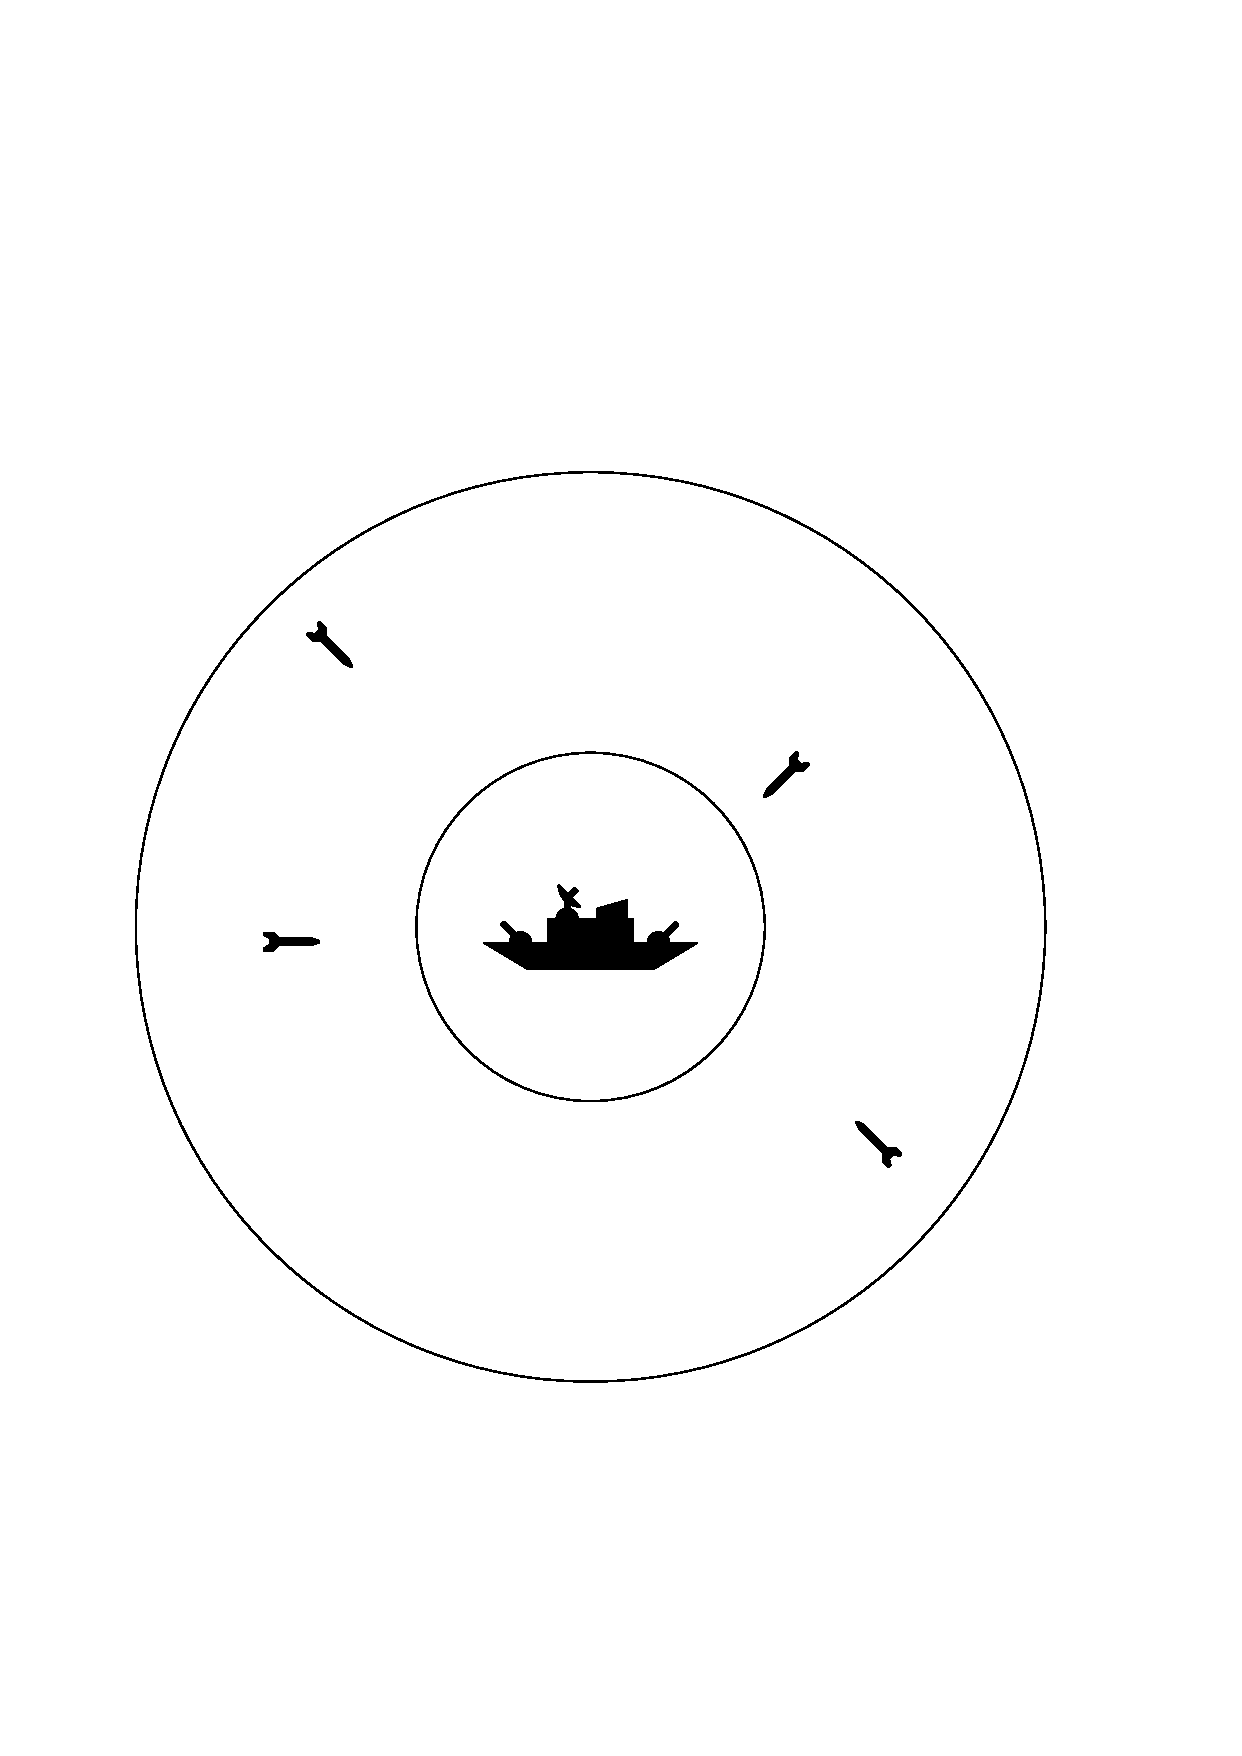
\includegraphics[width=.5\textwidth]{nereus}\\
  \caption{NEREUS: a Naval Environment for Resource Engagement in Unpredictable Situations.\label{fig:nereus}}
\end{figure}

Pour percevoir les missiles s'approchant, le navire poss�de un radar disposant d'une port�e de 3 km que nous supposerons parfait. Il poss�de �galement deux STIRs (radars d�di�s au guidage) permettant d'attacher aux menaces ennemies des missiles longue port�e ou une mitrailleuse lourde de port�e moyenne. Enfin, un syst�me de mitrailleuse l�g�re � courte port�e peut �galement �tre activ� si un missile adverse entre dans son champ d'action.

Nous consid�rons dans ce probl�me que la seule incertitude possible porte sur l'efficacit� des armes, � savoir la probabilit� que chacune d�truise la menace cibl�e. Ainsi, bien que discutable, l'hypoth�se est faite que le navire per�oit parfaitement le nombre et la position des missiles adverses.

Si l'on consid�re ce probl�me comme un probl�me stochastique de prise de d�cisions s�quentielles, il est possible de mod�liser au niveau d'un �tat les missiles adverses pr�sents et les armes disponibles pour les engager et mod�liser la dynamique de ces objets selon leurs capacit�s et les probabilit�s que chaque arme a de d�truire une menace. Le but est d'optimiser la probabilit� de survie du navire face � une attaque complexe pouvant comporter jusqu'� une dizaine de missiles.

Une formalisation math�matique et une solution � ce probl�me sont pr�sent�s dans le chapitre~\ref{chap:3} de cette th�se. La solution propos�e est essentiellement bas�e sur une combinaison des mod�les de planification classique sous incertitude avec une mod�lisation efficace des contraintes du probl�me, permettant un gain substantiel en terme de temps de calcul de la s�quence de d�cision optimale.

\subsection{Probl�mes multiagents}\label{ssect:multi}

Il a ensuite �t� sugg�r� d'�tudier le cas ou plusieurs de ces navires auraient � communiquer pour se d�fendre conjointement d'une attaque. Cependant, au vu de l'�tat actuel de la litt�rature multiagent pour r�soudre les probl�mes de planification d�centralis�e avec communication, et du peu de r�sultats de mod�lisation du domaine, nous nous sommes plut�t consacr�s � mod�liser la communication dans des probl�mes de coordination de la litt�rature plut�t que le probl�me de d�fense maritime. Voici quelques exemples de ces probl�mes.

\subsubsection{Patrouille de v�hicules a�riens autonomes}

Le probl�me de la patrouille est un tr�s vieux probl�me qui prend ses racines dans les probl�mes de la th�orie des graphes, notamment celui de la d�couverte d'un circuit hamiltonien~\citep{H.858}. Dans son expression la plus simple, il consiste � trouver un circuit hamiltonien sur un graphe de telle sorte � optimiser la mise � jour de l'information qui serait disponible � chaque n\oe ud. N�anmoins, si certains endroits doivent �tre mis � jour plus fr�quemment (par exemple si certains endroits sont plus ``sensibles'' ou ``� risque'' que d'autres), alors il est possible que le circuit hamiltonien ne soit plus la solution optimale et plusieurs agents a�riens autonomes doivent alors se coordonner pour conjointement maintenir une connaissance optimale de l'�tat courant de l'environnement.

\begin{figure}[htb]
\centering
  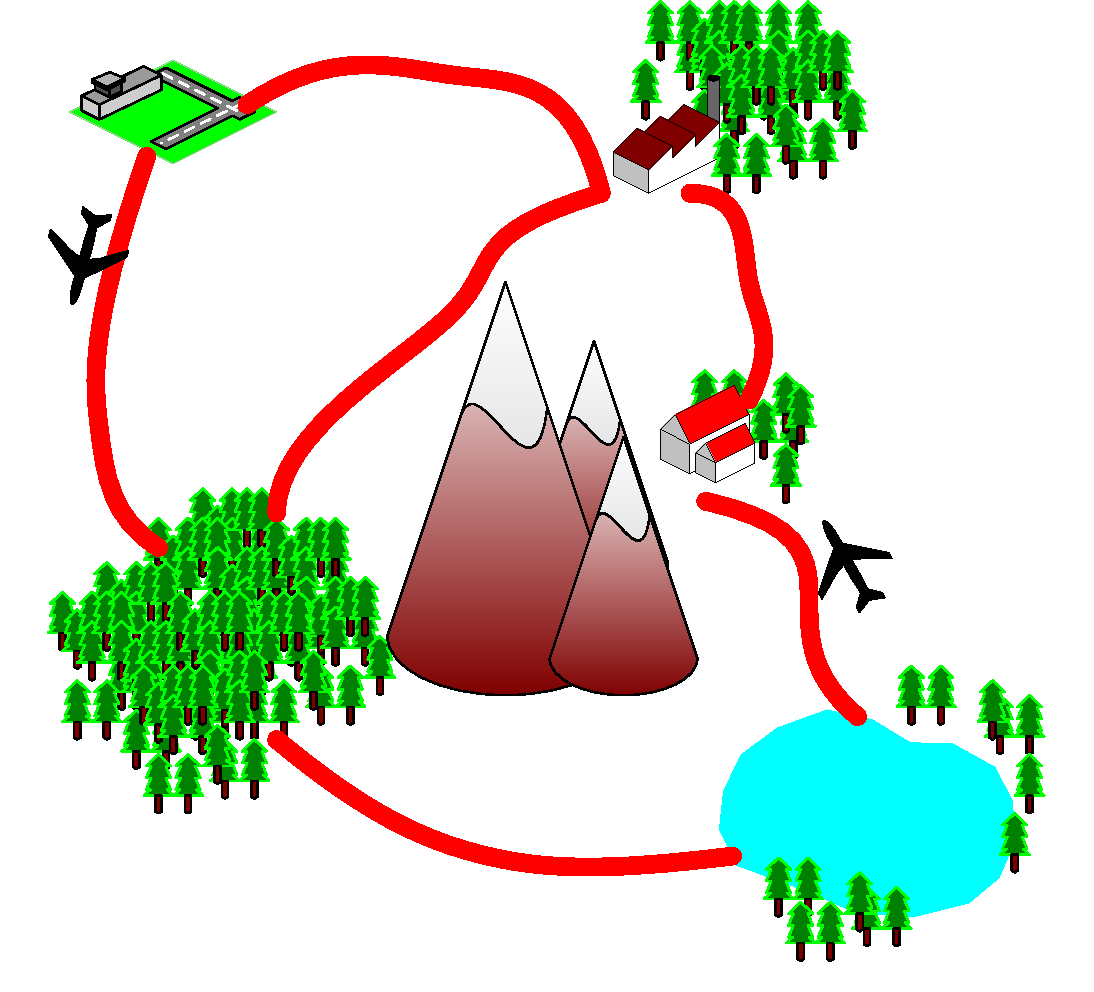
\includegraphics[width=.5\textwidth]{patrol}\\
  \caption{Un exemple de probl�me de patrouille � deux agents.\label{fig:patrol}}
\end{figure}

Dans ce contexte, les agents n'acc�dent pas � chaque instant � l'�tat complet de l'environnement, mais seulement au n\oe ud sur lequel ils se trouvent. Il leur faut donc maintenir une croyance sur la ``fra�cheur'' de l'information per�ue dans les n\oe uds pr�c�demment visit�s en consid�rant par exemple un taux d'obsolescence de l'information sur chaque sommet.

Du point de vue de la mod�lisation stochastique, le graphe � patrouiller et la position des agents sur ce graphe constituent l'�tat du syst�me complet. N�anmoins, les agents n'ont pas acc�s � cet �tat complet puisque nous faisons l'hypoth�se qu'ils ne savent pas si oui ou non leurs capteurs ont pu transmettre une information pertinente sur les sommets qu'ils viennent de patrouiller. D�s lors, les agents maintiennent une croyance sur l'�tat de ``fra�cheur'' de l'information et cherche � la maximiser �tant donn� une pond�ration initiale des sommets selon leur importance.

\subsubsection{Exp�dition \pac{mars} rovers}

\hyphenation{\'e-chan-til-lon-ner}
Initialement propos� par~\cite{SS.04} pour un seul agent, \emph{MultiAgent Rock Sample} (\textsc{mars}) d�crit comment plusieurs robots doivent interagir et communiquer pour �chantillonner de la mani�re la plus efficace possible un ensemble de roches ayant potentiellement une valeur scientifique (cf. figure~\ref{fig:mars}).

\begin{figure}[htb]
\centering
  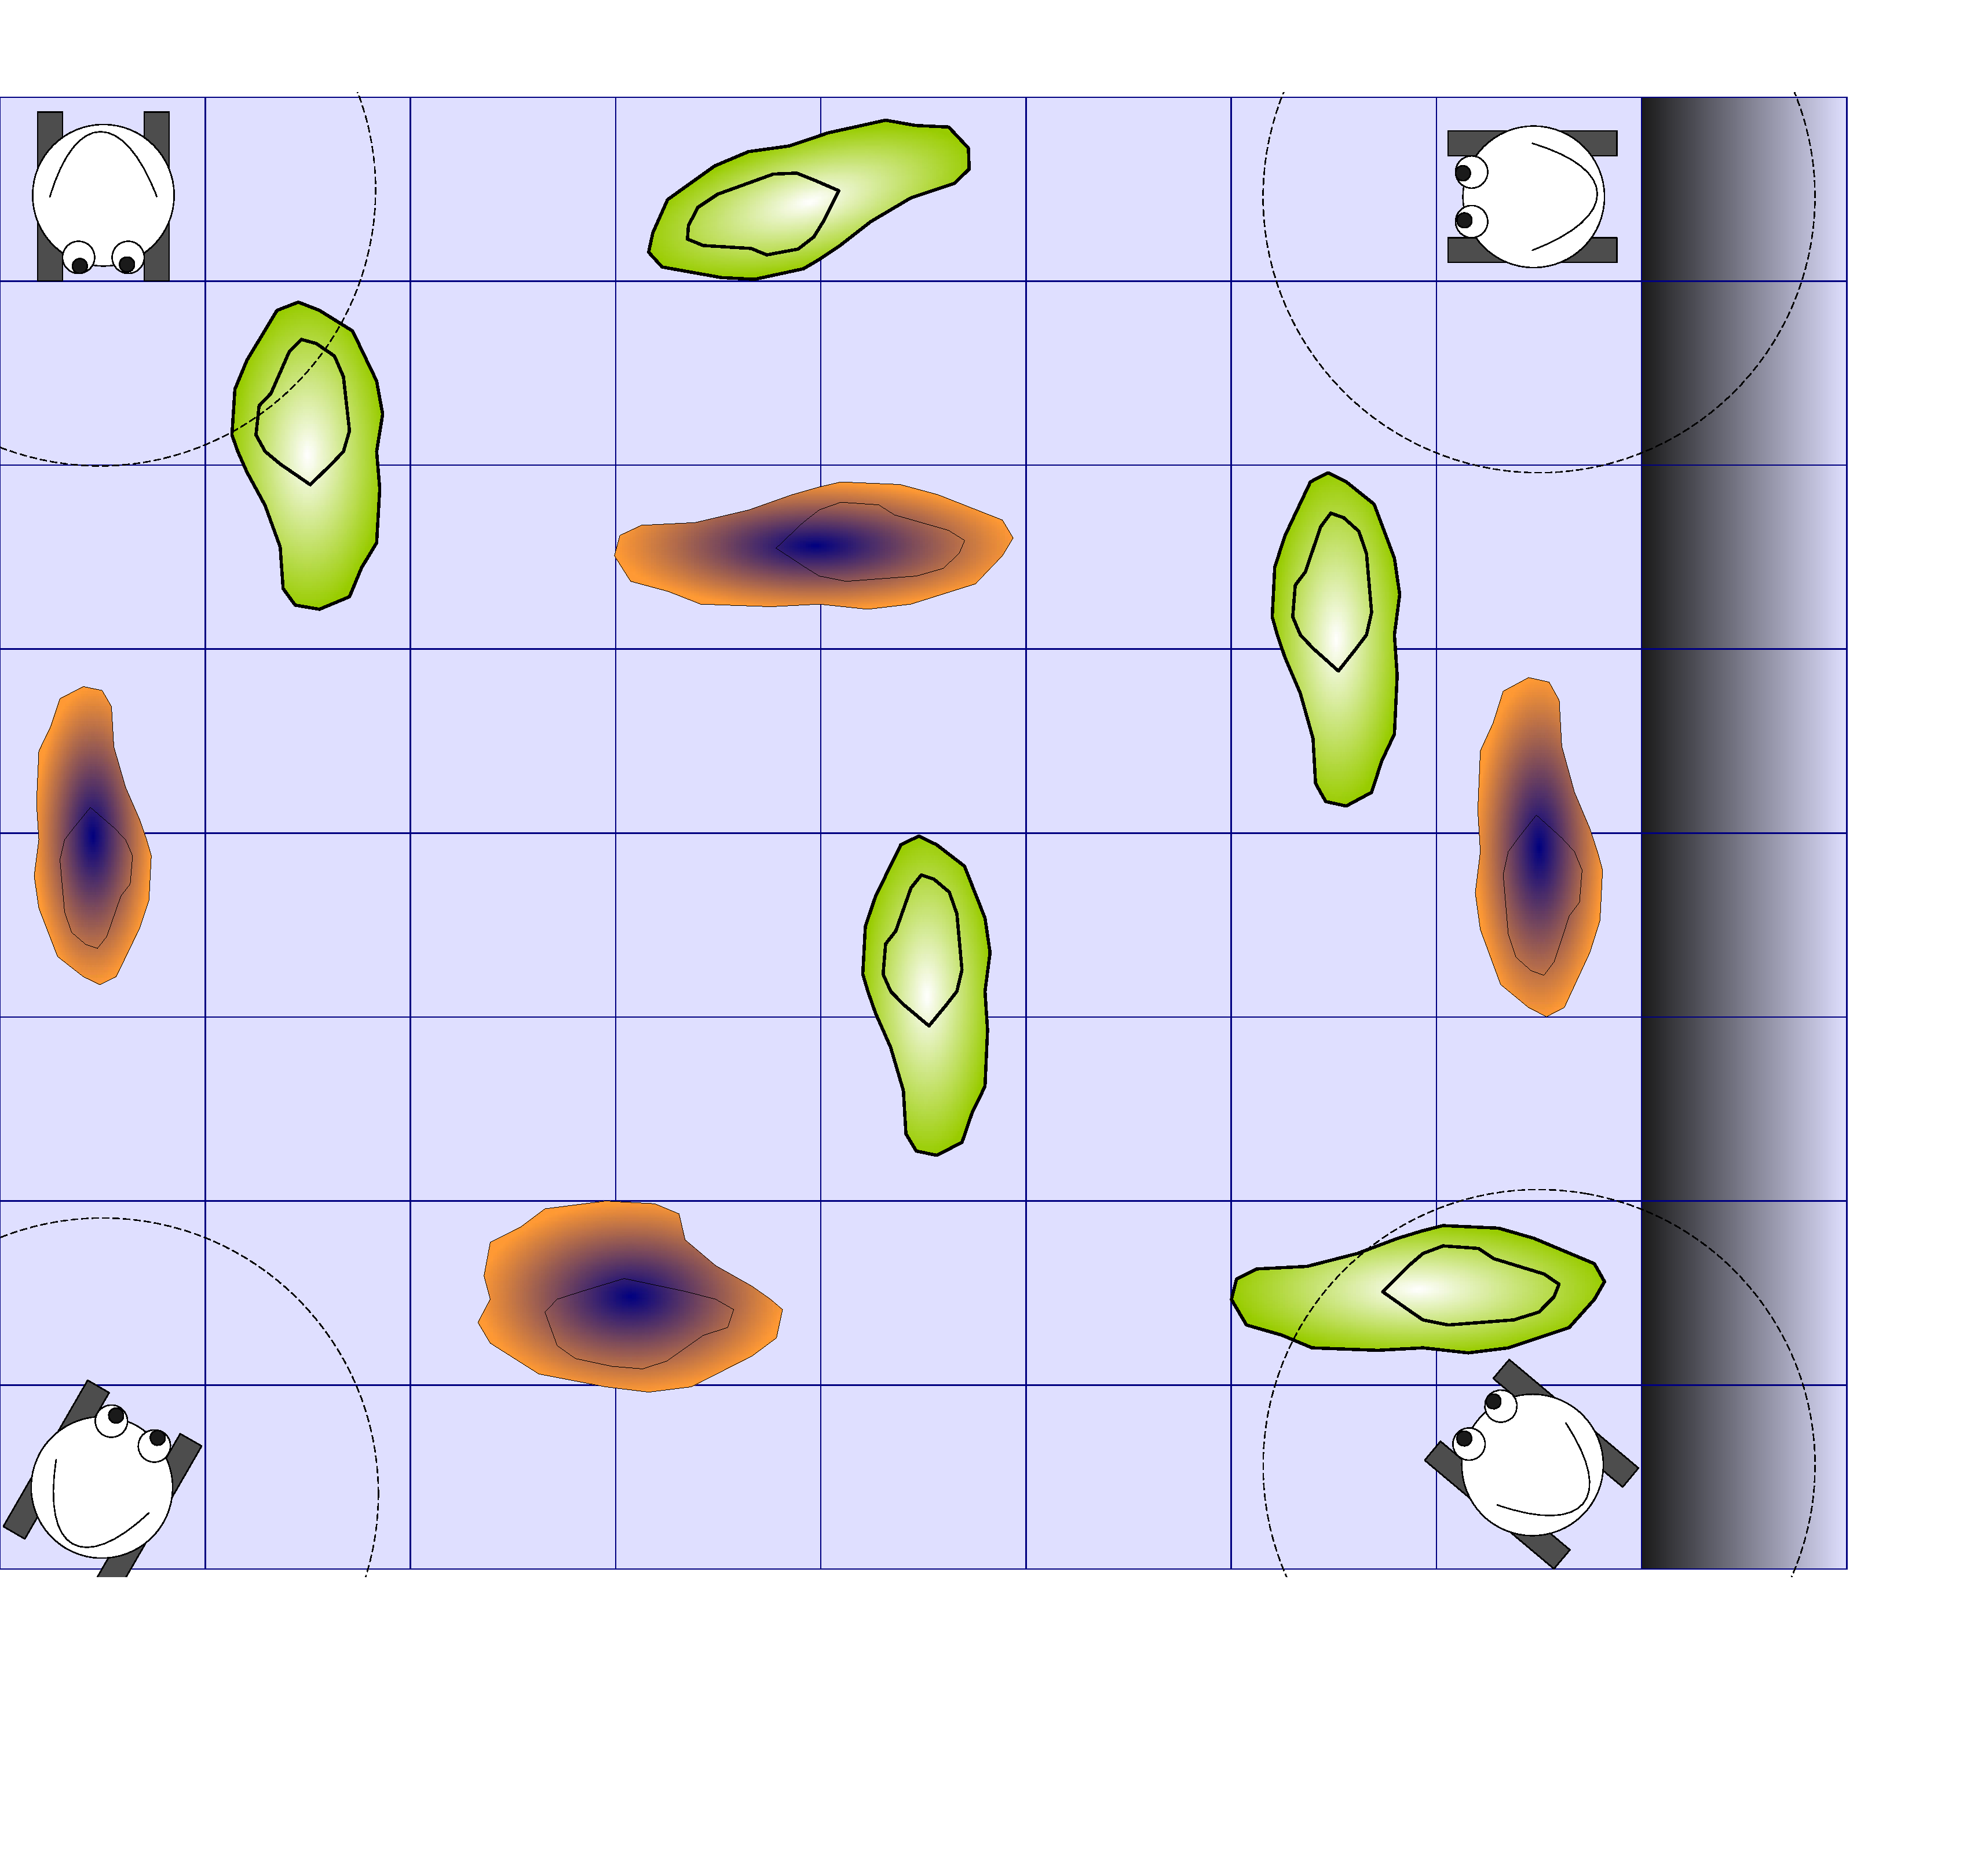
\includegraphics[width=.5\textwidth]{mars}\\
  \caption{Un exemple de probl�me d'exp�dition d'�chantillonnage de roche � 4 agents.\label{fig:mars}}
\end{figure}

\hyphenation{ro-ches}
On suppose que les agents connaissent leur position exacte dans l'environnement et que leurs d�placements sont d�terministes. L'incertitude r�side sur la valeur scientifique des roches � �chantillonner. Pour cela, un scanneur leur indique � chaque d�placement la qualit� des roches avoisinantes, avec une certaine confiance. Plus le robot est proche de la roche et plus le scanner est pr�cis quant � la qualit� de celle-ci. L'objectif est donc d'�chantillonner toutes les roches ayant une valeur scientifique puis de quitter l'environnement au plus vite par le c�t� droit de la grille.

L'�tat de ce probl�me se mod�lise ais�ment par la position des agents et la valeur scientifique (partiellement observable) des roches. La dynamique quant � elle, est extr�mement simple puisque quasiment d�terministe. Il convient enfin de maximiser le nombre de bonnes roches �chantillonn�es tout en minimisant le temps pass� � le faire.

\subsubsection{Les d�m�nageurs}\label{sect:demenageurs}

Ce probl�me a �t� propos� par~\cite{SZ.07} et d�crit le comportement de deux robots d�m�nageurs qui doivent ranger des boites dans un
environnement de type grille. Il y'a 3 boites dans l'environnement, deux petites et une grande. La grande n�cessite que les deux agents se
coordonnent pour pouvoir la pousser. Le but est d'amener une boite (et une seule) dans la zone but (en haut de la grille, voir figure
\ref{fig:coordbox}). L'optimal �tant bien sur d'apporter la grosse boite dans la zone but.

\begin{figure}[htb]
\centering
  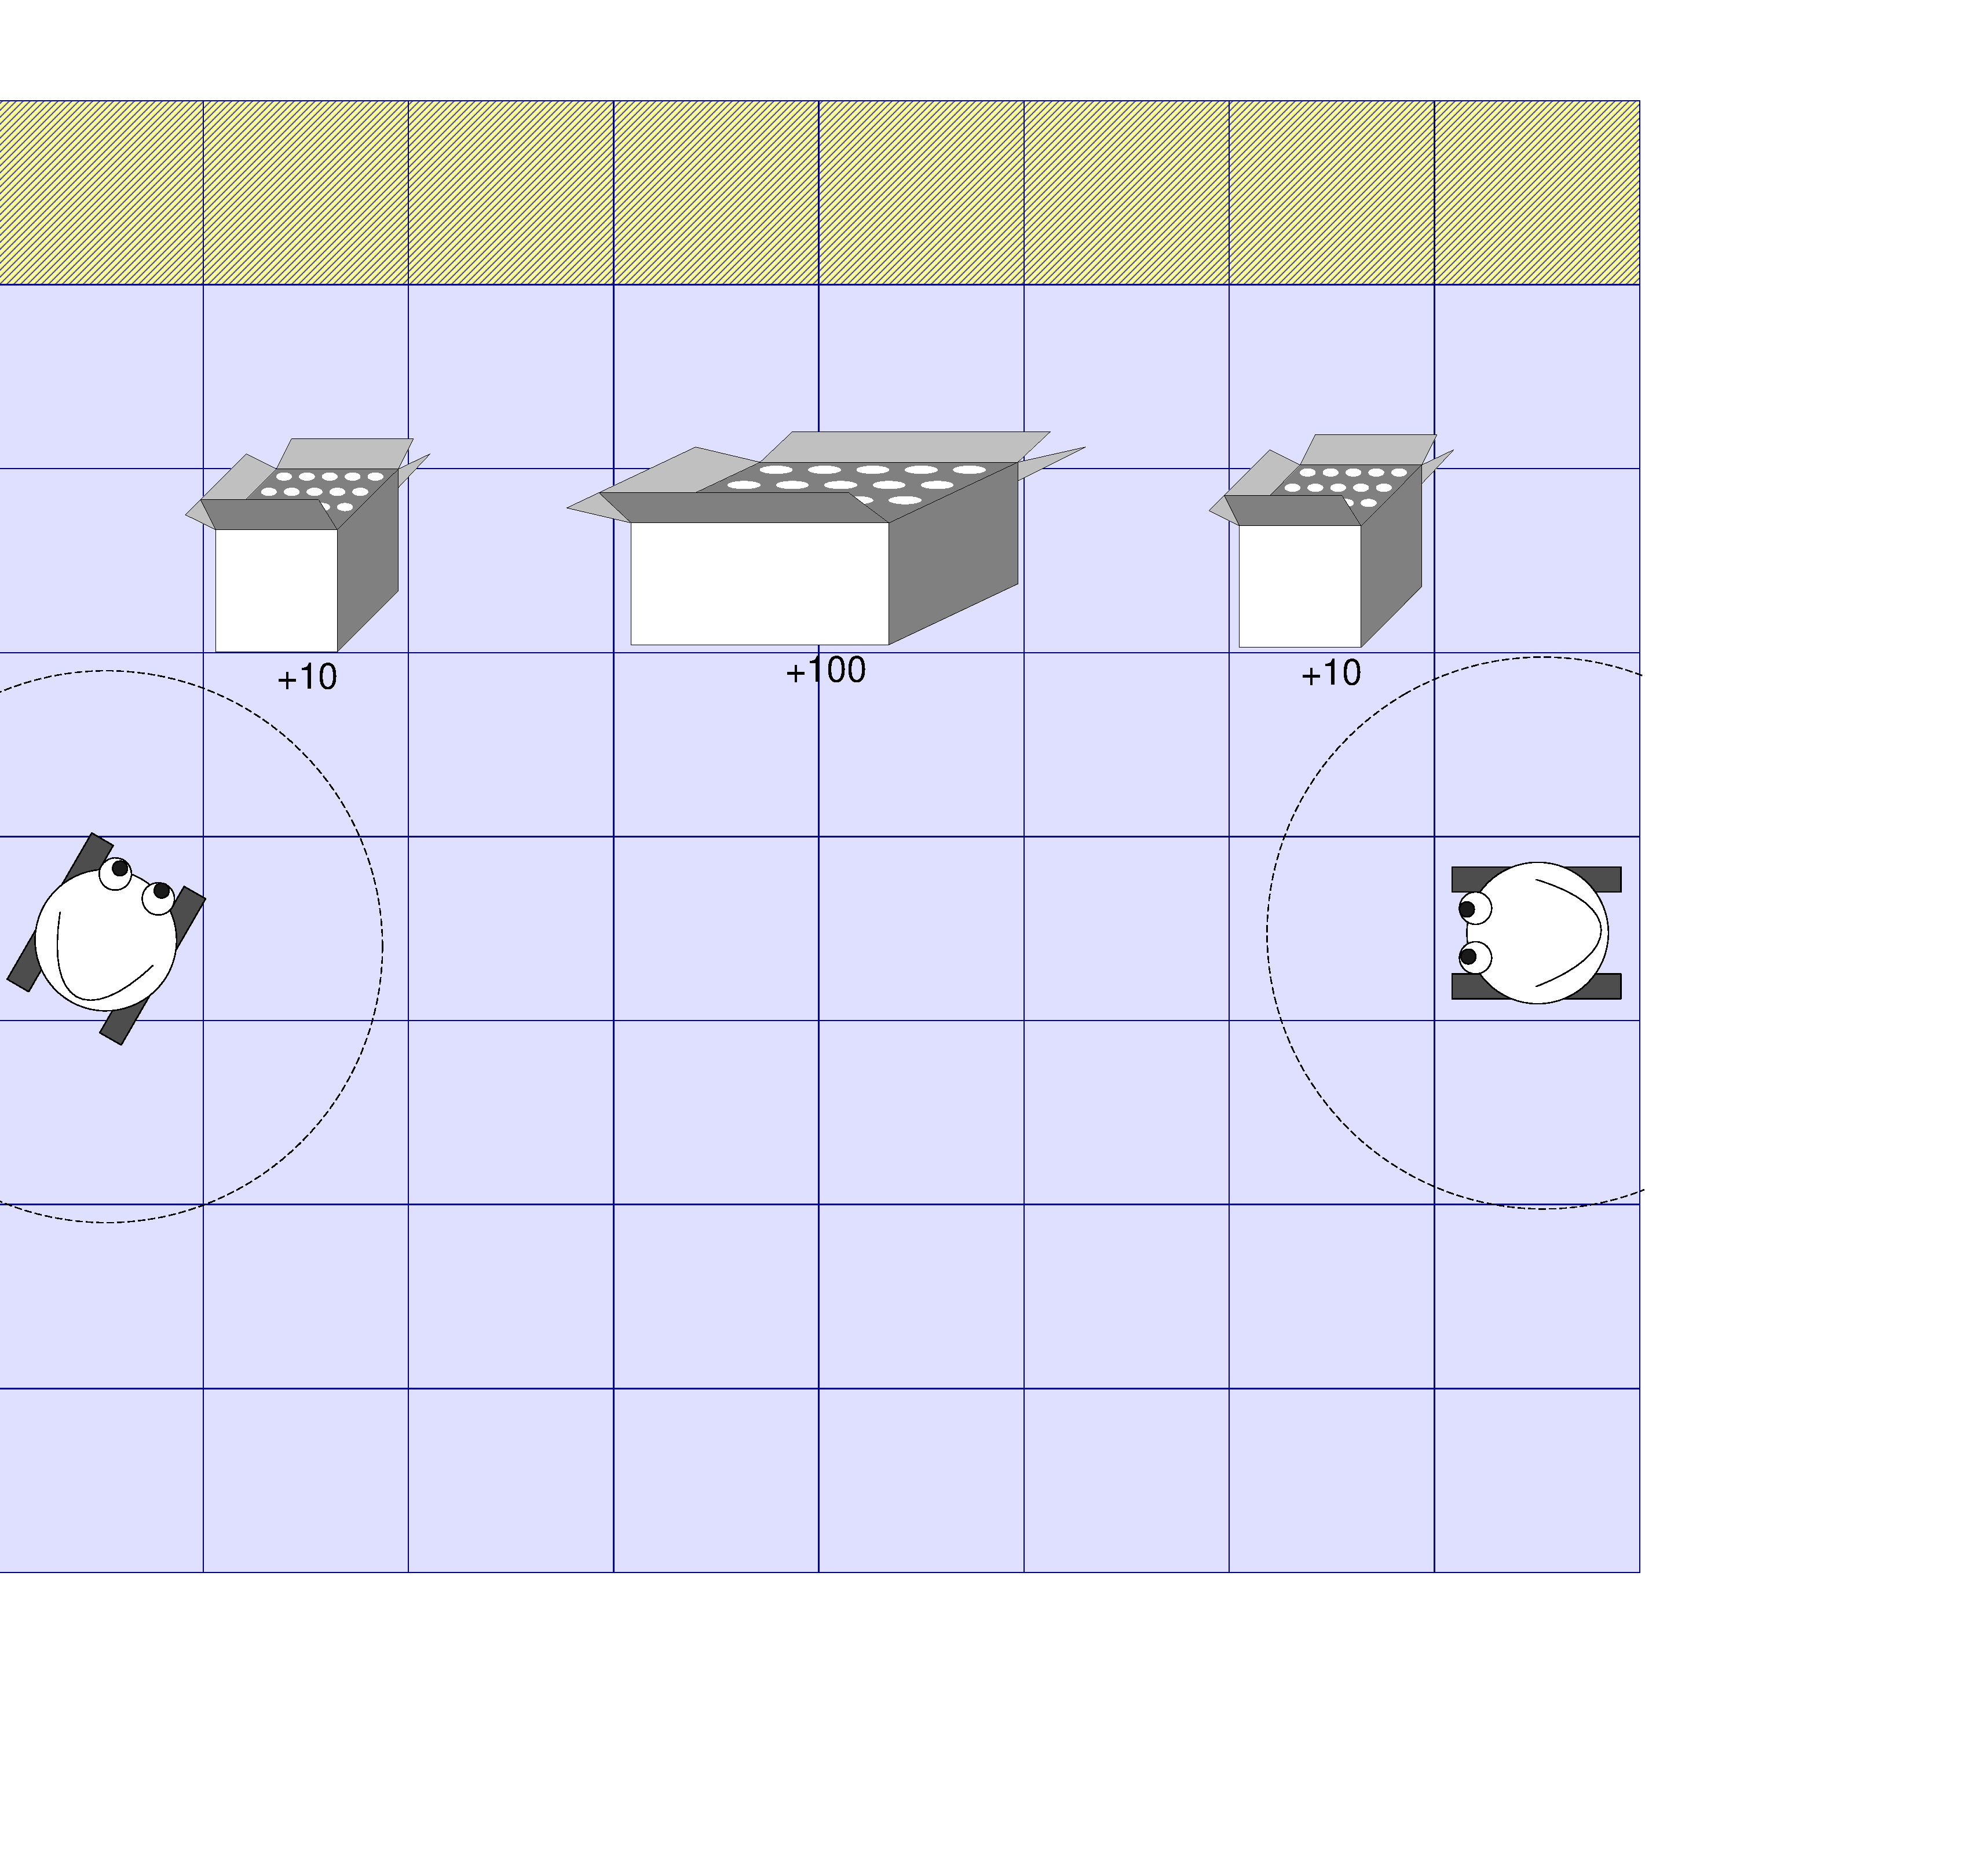
\includegraphics[width=.5\textwidth]{coordbox}\\
  \caption{Un exemple de probl�me de d�m�nageurs.}\label{fig:coordbox}
\end{figure}

Les agents n'ont ici qu'une vague id�e de leur position de d�part (ils savent seulement qu'ils sont � c�t� d'un mur). De plus, ils n'observent l'autre agent, un mur ou une boite que lorsque l'objet est exactement en face d'eux. Cette observabilit� tr�s limit�e rend le probl�me particuli�rement difficile lorsqu'en plus aucune communication n'est autoris�e.

L'�tat de ce probl�me contient la position des agents et des boites et la dynamique est simple. Chaque agent peut avancer dans la direction qui lui fait face ou peut faire un quart de tour sur place. Les petites boites peuvent �tre pouss�es dans toutes les directions par un agent, mais la grosse boite n�cessite la pouss�e coordonn�e des deux agents pour �tre d�plac�e. Le probl�me initial stipule que l'environnement est r�initialis� d�s qu'une boite atteint la zone en haut de la salle, mais on peut aussi essayer de trouver une strat�gie qui cherche simplement � minimiser le nombre d'�tapes permettant � la grosse boite d'�tre pouss�e en haut.

%Dans les probl�mes pr�sent�s ci-avant, plusieurs probl�mes ont �t� pr�sent�s o� les agents n'avaient acc�s qu'� une partie seulement de l'�tat et non plus � l'�tat complet du syst�me. d'autres probl�mes on �galement �t� pr�sent�s o� la dynamique pouvait �tre d�terministe. Voyons maintenant comment sont organis�es les contributions de cette th�se.

\section{Contributions de la th�se}

Cette th�se propose plusieurs nouvelles contributions au domaine de la prise de d�cisions s�quentielles sous incertitude. La figure~\ref{fig:contributions} repr�sente graphiquement la topologie des contributions effectu�es vis-�-vis des mod�les existants. Parmi ceux-ci, nous avons repr�sent� quatre mod�les majeurs de la prise de d�cisions s�quentielles sous incertitude qui seront plus amplement  d�taill�s au chapitre suivant.

Le processus d�cisionnel de Markov (\mdp) concerne un agent �voluant dans un environnement stochastique compl�tement observable. Plus complexe et plus g�n�ral, le \mdp partiellement observable (\pomdp) ajoute un degr� d'incertitude en n'autorisant la perception de l'�tat qu'au travers d'observations -- g�n�ralement bruit�es -- de celui-ci. Le \pomdp multiagent, quant � lui, �tend le \pomdp au contexte � plusieurs agents en faisant l'hypoth�se que ces agents communiquent librement. La suppression de cette derni�re hypoth�se m�ne au mod�le le plus complexe, le \pomdp d�centralis� (\decpomdp).

\begin{figure}[htb]
\centering
\begin{tikzpicture}[scale=1.1]%
%%MODELES
\filldraw[rounded corners,ultra thick,fill=gray!20,draw] (.8,0) rectangle (10.2,10.2);%%
\filldraw[rounded corners,ultra thick,vert,draw=green!70!blue] (1.1,4.1) rectangle (9.9,9.9);%%
\filldraw[rounded corners,ultra thick,bleu,draw=blue!70!green,dashed] (3.5,1) rectangle (9.9,3.8);%%
\filldraw[rounded corners,ultra thick,mauve,draw=blue!70!red] (3.5,5) rectangle (9.8,9.8);%%
\filldraw[rounded corners,ultra thick,fill=blue!30!green!5!white,draw=blue!50!green] (6,6) rectangle (9.7,9.7);%%
\filldraw[rounded corners,ultra thick,fill=orange,draw=red!70!green,dashed] (1.2,8.8) rectangle (9.6,9.6);%%
%%TEXTE MODELES
\node[font=\small] at (5.5,.5)  {Processus D�cisionnel de Markov}; %%
\node[font=\footnotesize] at (7,3)  {Probl�mes de Satisfaction}; %%
\node[font=\footnotesize] at (7,2)  {de Contraintes Markoviens}; %%
\node[font=\small] at (5.5,4.5)  {Partiellement Observable}; %%
\node[font=\footnotesize] at (8.25,5.3)  {Multiagent}; %%
\node[font=\footnotesize] at (8.25,6.3)  {D�centralis�}; %%
\node[font=\footnotesize] at (5.4,9.2)  {Quasi-D�terministe}; %%
%%ALGOS+BORNES
%\node [decorate, decoration=zigzag, fill=yellow!20,draw,circle, font=\scriptsize] at (3,3) {\textsc{r-frtdp}};%%
%\node [decorate, decoration=zigzag, fill=yellow!20,draw,circle, font=\scriptsize] at (6,6) {Rollout};%%
\node [fill=yellow!20,draw,circle, font=\scriptsize] at (3,3) {\textsc{r-frtdp}};%%
\node [fill=yellow!20,draw,circle, font=\scriptsize] at (6,6) {dRollout};%%
%\filldraw[rounded corners,thick,fill=gray!1.2,draw] (1,1.3) rectangle (3,2);%%
\node[thick,dashed,fill=gray!1,draw,font=\tiny] at (2.5,2.5)  {+ Bornes}; %%
%\filldraw[rounded corners,thick,fill=gray!1,draw] (2.5,8.35) rectangle (9.5,8.95);%%
%\node[font=\tiny] at (6,8.65)  {+ Bornes PAC}; %%
\node[thick,dashed,fill=gray!1,draw,font=\tiny] at (8.3,9.2)  {+ Bornes PAC}; %%
%%PROBLEMES
%\filldraw [decorate, decoration=bumps, fill=gray!1,draw] (2.2,1.2) rectangle (4,1.6);%%
\node[font=\scriptsize,fill=gray!1,draw,cloud,aspect=2,inner sep=0pt] at (3.1,1.4)  {\textsc{nereus}}; %%
%\filldraw [decorate, decoration=bumps, fill=gray!1,draw] (3.7,7.95) rectangle (5.8,8.45);%%
\node[font=\scriptsize,fill=gray!1,draw,cloud,aspect=2,inner sep=-3pt] at (4.75,8.2)  {Patrouille}; %%
%\filldraw [decorate, decoration=bumps, fill=gray!1,draw] (3.7,7.05) rectangle (5.8,7.55);%%
\node[font=\scriptsize,fill=gray!1,draw,cloud,aspect=2,inner sep=0pt] at (4.75,7)  {\textsc{mars}}; %%
%\filldraw [decorate, decoration=bumps, fill=gray!1,draw] (6.7,7.55) rectangle (9.2,8.05);%%
\node[font=\scriptsize,fill=gray!1,draw,cloud,aspect=2,inner sep=-5pt] at (7.95,7.8)  {D�m�nageurs}; %%
%\node[font=\small] at (3,2)  {Text}; %%
%%GRILLE
%\draw[step=1cm,color=gray,very thin] (0,0) grid (10,10);%%
%%LEGENDE
\filldraw[rounded corners,thick,fill=gray!1,draw] (11,4.5) rectangle (15,10);%%
\node[font=\footnotesize] at (13,9.5)  {L�gende}; %%
\filldraw[rounded corners,ultra thick,fill=gray!15,draw] (11.2,8.1) rectangle (14.8,8.9);%%
\node[font=\footnotesize] at (13,8.5)  {Mod�le Existant}; %%
\filldraw[rounded corners,ultra thick,fill=gray!15,draw,dashed] (11.2,7.1) rectangle (14.8,7.9);%%
\node[font=\footnotesize] at (13,7.5)  {Mod�le Propos�}; %%
%\filldraw[decorate, decoration={zigzag,amplitude=.5mm}, fill=yellow!20,draw] (11.2,6.1) rectangle (14.8,6.9);%%
%\filldraw[fill=yellow!20,draw] (11.2,6.1) ellipse (14.8,6.9);%%
\node[font=\footnotesize,fill=yellow!20,draw,ellipse] at (13,6.5)  {Algorithme}; %%
%\filldraw[decorate, decoration=bumps, fill=gray!1,draw] (11.2,5.15) rectangle (14.8,5.75);%%
\node[font=\footnotesize,fill=gray!1,draw,cloud, aspect=2,inner sep=-5pt] at (13,5.25)  {Probl�me}; %%
\end{tikzpicture}
  \caption{Repr�sentation hi�rarchique des contributions de la th�se.\label{fig:contributions}}
\end{figure}

\hyphenation{d\'e-cen-tra-li-s\'e}
Cette th�se contribue � plusieurs niveaux de cette hi�rarchie:
\begin{description}
\item[Au niveau des \mdps:]~\\
    \begin{itemize}\vspace{-15pt}
    \item Nous avons propos�, en collaboration avec Pierrick Plamondon, un algorithme de r�solution des probl�mes d'allocation de ressources sous incertitude (\textsc{r-frtdp}), ainsi que des bornes serr�es pour ce type de probl�me;
    \item Nous avons �galement propos� un mod�le prenant en compte une connaissance � priori des contraintes sur les d�cisions possibles ainsi que l'�volution de l'algorithme pr�c�dent pour ce nouveau mod�le. Des r�sultats th�oriques et exp�rimentaux sont fournis et discut�s dans ce contexte dans le chapitre~\ref{chap:3};
    \end{itemize}
\item[Au niveau des \pomdps:]~\\
    \begin{itemize}\vspace{-15pt}
        \item Nous avons propos� un nouveau mod�le appel� quasi-d�terministe pr�sent� dans le chapitre~\ref{chap:4};
        \item Des mod�les contraints d'observations pour ce mod�le sont �galement propos�s, permettant la d�rivation de nouveaux r�sultats de complexit� associ�s � une borne probablement approximativement correcte (\textsc{pac});
    \end{itemize}
\item[Au niveau des \mpomdps:]~\\
    \begin{itemize}\vspace{-15pt}
    \item Dans la deuxi�me partie du chapitre~\ref{chap:4}, nous avons propos� l'extension du mod�le quasi-d�terministe au contexte multiagent et nous l'avons ensuite appliqu� aux probl�mes de coordination d'agents de patrouille et d'exploration \textsc{mars};
    \item Pour cela, un algorithme de m�lange de politiques locales a �t� propos� en collaboration avec Jean-Samuel Marier pour r�soudre les deux probl�mes pr�c�dents;
    \end{itemize}
\item[Au niveau des \decpomdps:]~\\
    \begin{itemize}\vspace{-15pt}
    \item Nous avons propos� un algorithme d'approximation d�centralis� (dRollout) ainsi que son application au probl�me des d�m�nageurs. Diff�rents r�sultats sont pr�sent�s dans le chapitre~\ref{chap:5} selon certaines hypoth�ses de mise � jour des �tats de croyance;
    \item Le mod�le quasi-d�terministe est �galement d�taill� dans le cas d�centralis�, des r�sultats th�oriques sont d�riv�s et l'application � un nouveau probl�me jouet d�centralis� sous communication non fiable d�montre de son efficacit� exp�rimentale.
    \end{itemize}
\end{description}

\section{Organisation de la th�se}

� partir de cette topologie, nous avons organis� cette th�se comme suit:
\begin{description}
\item[Le Chapitre~\ref{chap:2}] pr�sente la base des processus d�cisionnels de Markov monoagents et multiagents. Il introduit �galement quelques algorithmes basiques de la litt�rature et certains r�sultats choisis de complexit� pour ces mod�les;
\item[Le Chapitre~\ref{chap:3}] pr�sente les contributions apport�es aux processus d�cisionnels de Markov � un seul agent et sous observabilit� compl�te dans le cadre du probl�me d'allocation de ressources pr�sent� � la section~\ref{ssect:nereus}. � cette fin, il introduit le probl�me d'allocation d'armes � des cibles puis les probl�mes de satisfaction de contraintes. Le mod�le propos� est ensuite d�taill� puis analys� th�oriquement. Finalement, un algorithme adapt� pour ce mod�le, ainsi que de nouvelles bornes utilis�es comme heuristiques, sont pr�sent�s et analys�s empiriquement;
\item[Le Chapitre~\ref{chap:4}] pr�sente le nouveau mod�le quasi-d�terministe pour certains probl�mes partiellement observables monoagents et multiagents. Une borne \textsc{pac} sur l'horizon maximal de planification est d�riv�e sous certaines conditions permettant l'obtention de r�sultats de complexit� int�ressants. Ces mod�les sont ensuite utilis�s pour la repr�sentation des probl�mes formalis�s � la section~\ref{ssect:multi}. Quelques r�sultats exp�rimentaux sont �galement pr�sent�s;
\item[Le Chapitre~\ref{chap:5}] pr�sente l'algorithme de r�solution approch�e en ligne dans le cas d�centralis� bas� sur un algorithme de type Rollout~\citep{B.00}. Une �tude empirique de la mise � jour de l'�tat de croyance est �galement r�alis�e sur le probl�me des d�m�nageurs;
\item[Le Chapitre~\ref{chap:conclusion}] conclut cette th�se et pr�sente quelques travaux futurs.
\end{description}









%*****************************************************************************************************************************

%\subsection*{Agents}
%
%Il est possible de rencontrer des probl�mes o� la d�cision � prendre ne puisse se faire de mani�re centralis�e. Par exemple lorsque qu'une �quipe de v�hicules autonomes patrouillent un territoire, chacun fait face � des situations locales qui n'ont que peu d'influence sur le comportement des autres et o� la d�centralisation de la solution est pr�f�rable. Dans ce contexte \emph{multiagents}, on diff�rencie trois domaines en particuliers:
%\begin{itemize}
%\item \emph{La th�orie des jeux} qui �tudie le comportement d'un agent en \emph{comp�tition} avec d'autres agents. Dans l'exemple de la patrouille on pourrait imaginer des v�hicules autonomes ennemis qui tenteraient d�truire les patrouilleurs.
%\item \emph{La Coop�ration et la coordination} �tudient les probl�mes o� les agents tentent d'atteindre un but commun et connu de tous.
%\item \emph{L'�mergence et intelligence d'essaim} �tudie les probl�mes o� un tr�s grand nombre d'agents tr�s simples tentent de r�aliser un comportement complexe �mergent seulement des interactions locales entre les agents.
%\end{itemize}

%\subsection*{Crit�re d'optimalit�}

%Finalement, selon la nature du probl�me, il est n�cessaire de d�finir un crit�re formalisant les buts et les d�sirs de chacun des agents. Ce crit�re peut �tre un crit�re de \emph{satisfaction} ou bien d'\emph{optimisation} selon que l'on cherche seulement � trouver une situation satisfaisante ou alors � ordonner les solutions puis � prendre la plus satisfaisante (l'optimale). Il est �galement possible de ne trouver qu'une solution proche de la solution optimale mais ``suffisamment'' satisfaisante pour l'agent. Tout cela est d�termin� par le crit�re d'optimalit� du probl�me.

%\subsection*{En r�sum� ...}
%
%R�capitulons rapidement les diff�rents domaines que nous avons �nonc�s pour nous focaliser le domaine bien particulier pour lequel nous avons contribu�. Nous allons discuter dans cette th�se:
%\begin{itemize}
%\item d'un probl�me de d�cision s�quentiel
%\item impliquant un ou plusieurs agents interagissant avec
%\item un environnement � variables et � �v�nements discrets mais partiellement observables,
%\item avec un mod�le stochastique de la dynamique, explicitement donn� initialement,
%\item et cherchant � maximiser un crit�re d'optimisation unique par interaction avec l'environnement.
%\end{itemize}
%

%*****************************************************************************************************************************

%\subsection{En r�sum� : caract�ristiques des probl�mes}
%
%Dans les probl�mes pr�sent�s ci-avant, nous avons vu plusieurs probl�mes ou le ou les agents n'avaient acc�s qu'� une partie seulement de l'�tat et non plus � l'�tat complet du syst�me. Nous avons �galement vu des probl�mes ou la dynamique pouvait �tre d�terministe. Nous allons donc faire ici un bilan des caract�ristiques des probl�mes pr�sent�s en vue de pr�parer la pr�sentation des contributions de cette th�se :
%\begin{description}
%\item[Probl�me �pisodique / s�quentiel :] Une premi�re caract�ristique des probl�mes concerne le degr� d'influence de chacune des d�cision sur les d�cisions � venir. Lorsque le probl�me est �pisodique, l'agent per�oit sa situation, trouve la meilleure action � entreprendre dans cette situation et l'ex�cute. Une nouvelle situation est alors per�ue, ind�pendamment de l'action entreprise. Dans le cas s�quentiel, en revanche, l'action effectu�e par l'agent influence le prochain �tat du syst�me et les �tats subs�quents. Il devient donc n�cessaire de raisonner sur toutes les s�quences futures d'�tats possibles pour �valuer une action convenablement. Seuls ces derniers types de probl�mes seront abord�s dans cette th�se.
%\item[Environnement discret / continu :] Lors d'une prise de d�cision, l'agent doit souvent prendre en compte des quantit�s aussi bien discr�tes que continues. Lorsqu'il s'agit d'orienter un v�hicule ou de choisir la pouss�e d'un moteur par exemple, l'agent doit choisir parmi une infinit� de possibilit�. Alors que lorsqu'il se d�place sur une grille, ou un graphe, ses diff�rents choix sont souvent �num�rables. La majorit� des probl�mes que nous consid�rerons dans cette th�se sont discrets.
%\item[Environnement contraint / libre :] Il est fr�quent de trouver dans la d�finition de probl�me la pr�sence d'un connaissance � priori qui contraint la prise de d�cision ou les situations possibles. Dans le cadre de la defense maritime par exemple, les armes n'ont pas une port�e infinie. Ces contraintes peuvent �tre alors utilis�es pour am�liorer la recherche d'une solution optimale au probl�me consid�r�.
%\item[Dynamique d�terministe / stochastique :] Lorsque l'action d'un agent peut �ventuellement �chouer ou mener � plus d'une situation possible, alors on parle de probl�me stochastique. Dans le cas inverse, si l'action d'un agent dans un �tat conduit toujours dans le m�me �tat suivant, alors l'environnement est consid�r� d�terministe. Cette th�se est particuli�rement int�ress�e par les probl�mes stochastiques bien que certains r�sultats pr�sent�s ne s'appliquent qu'aux probl�mes d�terministes.
%\item[Observabilit� compl�te / partielle :] L'observabilit� de l'environnement est un des axes majeurs de cette th�se. En effet, la complexit� d'un probl�me est tr�s souvent rattach�e � la capacit� que l'agent a � d�terminer pr�cis�ment dans quel �tat is se trouve. L'observabilit� compl�te est d�finie d�s lors que l'agent � acc�s � toute l'information n�cessaire pour prendre sa d�cision. Dans le cas inverse, o� certaines parties de l'�tat ne sont pas observ�es ou le sont avec un certain bruit, l'agent doit ainsi raisonner sur une croyance sur les valeurs que peuvent prendre ces parties d'�tat.
%\item[Un ou plusieurs agents :] La derni�re caract�ristique du probl�me concerne le nombre d'agents dans l'environnement. Dans cette th�se, nous ne consid�rerons pas le cas ou plusieurs agents travaillent les uns \emph{contre} les autres, n�anmoins, nous serons amen�s � consid�rer des probl�mes o� plusieurs agents devront coop�rer en vue d'attendre un objectif commun. La premi�re partie de cette th�se focalise plus sur les probl�mes monoagents alors que la seconde s'oriente vers les probl�mes de d�cisions distribu�es. La principale difficult� associ�e � la distribution de la d�cision est essentiellement due au fait que chacun des agents doit raisonner sur toutes les actions possibles des autres agents augmentant consid�rablement le nombre d'options possibles.
%\end{description}

\newpage\phantom{a}

%Bases th�orique MDPs -> DecPOMDPs
\chapter{Bases sur les processus d�cisionnels de Markov}

% \emph{�En essayant continuellement on finit par r�ussir. Donc : plus �a rate, plus on a de chance que �a marche.�}
% \begin{flushright}Les Shadoks -- Jacques Rouxel\end{flushright}
% \bigskip
 \emph{�Toute connaissance d�g�n�re en probabilit�.�}
 \begin{flushright}David Hume\end{flushright}
 \bigskip


\label{chap:2}
\begin{summary}
Ce chapitre introduit les bases th�oriques des mod�les probabilistes, c'est � dire le formalisme math�matique permettant la
description de probl�mes de d�cisions s�quentielles et stochastiques appel�s \emph{Processus D�cisionnels de Markov} (en anglais, \emph{Markov Decision Processes} ou \mdp). Dans une premi�re partie, les mod�les fondamentaux centralis�s sont pr�sent�s � la mani�re de \cite{S.06} avant de pr�senter ceux destin�s aux probl�mes impliquant plusieurs agents comme l'ont fait \cite{SZ.05}.
\end{summary}

\section{Mod�les pour un agent}
Les \mdps ont �t� introduits et popularis�s � la fin des ann�es cinquante par \cite{B.57} et \cite{H.60}. Ce formalisme se
base sur un mod�le � la fois tr�s g�n�ral et assez abstrait pour pouvoir �tre appliqu� � des probl�mes vari�s, mais cependant restreint de
par ses hypoth�ses sur le caract�re totalement observable de l'environnement et sur le contr�le disponible strictement centralis�.

\subsection{Processus d�cisionnel de Markov (\pac{mdp})}
Nous pr�sentons ici rapidement le formalisme \mdp ainsi que quelques algorithmes fondamentaux permettant leur r�solution. Notons qu'une
introduction exhaustive des \mdps peut �tre trouv�e dans le livre de \cite{P.94}.

\subsubsection{Formalisme}
\begin{definition}(\mdp)
Un \mdp est d�fini par un tuple $\la \Sta, \Act, \Tra, \Rew \ra$, o�:
\begin{itemize}
\item $\Sta$ est un ensemble fini d'\emph{�tats} $s \in \Sta$;
\item $\Act$ est un ensemble fini d'\emph{actions} $a \in \Act$;
\item $\Tra(s,a,s'): \Sta \times \Act \times \Sta \mapsto [0,1]$ est la \emph{probabilit� de transition} du syst�me de l'�tat $s$ vers l'�tat $s'$ apr�s l'ex�cution de l'action $a$;
\item $\Rew(s,a): \Sta \times \Act \mapsto \mathds{R}$ est la \emph{r�compense} produite par le syst�me lorsque l'action $a$ est ex�cut�e dans l'�tat $s$.
\end{itemize}
\end{definition}

La propri�t� fondamentale de ce formalisme est \emph{la propri�t� de Markov}. Elle garantit que la probabilit� de transition d'un �tat $s$
vers un �tat $s'$ sous l'effet d'une action $a$ est ind�pendante du pass�:
\begin{equation*}
\pr(s_{t+1} = s' | s_0, a_0, s_1, a_1, ..., s_t, a_t) = \pr(s_{t+1} = s' | s_t, a_t)
\end{equation*}
Par cons�quent, l'�tat courant et la derni�re action constituent toujours une information suffisante pour la pr�diction de l'�volution du syst�me.

Une repr�sentation graphique d'un \mdp est donn�e par la figure~\ref{fig:mdp}. Les cercles repr�sen-tent les variables non contr�lables (les �tats), les carr�s repr�sentent les variables de d�cisions (les actions) et les losanges les r�compenses re�ues. Un lien entre deux variables induit une table relationnelle (par exemple de probabilit�) qui associe � chaque couple de valeur possible pour ces variables sa probabilit� de vraisemblance. Les liens en tirets indiquent la connaissance disponible par l'agent au moment de prendre la d�cision (dans l'exemple de la figure~\ref{fig:mdp}, l'agent conna�t l'�tat du syst�me).

\begin{figure}[h!tb]
        \begin{center}
        \begin{tikzpicture}[scale=.7]%
        %\draw[step=1cm,color=gray,very thin] (-5,-1) grid (9,5);%%
        \begin{scope}[shape=diamond,inner sep=.02cm,minimum size=0.8cm]
        \tikzstyle{every node}=[draw,font=\footnotesize] %%
        \node (r1) at (-9,-3)  {$r^1$}; %%
        \node (r2) at (-4,-3)  {$r^2$}; %%
        \node (r3) at (1,-3)  {$r^3$}; %%
        \node (rt) at (6,-3)  {$r^T$}; %%
        \end{scope}%
        \begin{scope}[shape=circle,inner sep=.02cm,fill=white,minimum size=0.8cm]
        \tikzstyle{every node}=[draw,font=\footnotesize] %%
        \node (s0) at (-12,0)  {$\cs^0$}; %%
        \node (s1) at (-7,0)  {$\cs^1$}; %%
        \node (s2) at (-2,0)  {$\cs^2$}; %%
        \node (s3) at (3,0)  {$\cs^3$}; %%
        \node (st) at (8,0)  {$\cs^T$}; %%
        \end{scope}
        \begin{scope}[shape=rectangle,inner sep=.05cm,fill=white,minimum size=0.8cm]
        \tikzstyle{every node}=[draw,font=\small] %%
        \node (a11) at (-10,3)  {$\ca^1$}; %%
        \node (a12) at (-5,3)  {$\ca^2$}; %%
        \node (a13) at (0,3)  {$\ca^3$}; %%
        \node (a1t) at (5,3)  {$\ca^T$}; %%
        \end{scope}
        \draw[->,-latex] (s0)--(s1);  %%
        \draw[->,-latex] (s1)--(s2); %%
        \draw[->,-latex] (s2)--(s3); %%
        \draw[->,-latex,dotted,thick] (s3)--(st); %%
        \draw[->,-latex] (a11)-- +(1.5,-3) --(s1);  %%
        \draw[->,-latex] (a12)-- +(1.5,-3) --(s2);  %%
        \draw[->,-latex] (a13)-- +(1.5,-3) --(s3);  %%
        \draw[->,-latex] (a1t)-- +(1.5,-3) --(st);  %%
        \draw[->,-latex,dashed] (s0)--(a11); %%
        \draw[->,-latex,dashed] (s1)--(a12); %%
        \draw[->,-latex,dashed] (s2)--(a13); %%
        \draw[->,-latex,loosely dashed,thick] (s3)--(a1t); %%
        \draw[->,-latex,double] (s1)--+(-2,-1)--(r1);  %%
        \draw[->,-latex,double] (a11)--+(1,-4)--(r1);  %%
        \draw[->,-latex,double] (s2)--+(-2,-1)--(r2);  %%
        \draw[->,-latex,double] (a12)--+(1,-4)--(r2);  %%
        \draw[->,-latex,double] (s3)--+(-2,-1)--(r3);  %%
        \draw[->,-latex,double] (a13)--+(1,-4)--(r3);  %%
        \draw[->,-latex,double] (st)--+(-2,-1)--(rt);  %%
        \draw[->,-latex,double] (a1t)--+(1,-4)--(rt);  %%
        \end{tikzpicture}%
        \caption{Repr�sentation graphique d'un \mdp.\label{fig:mdp}}
    \end{center}
\end{figure}

Ex�cuter un \mdp revient � observer en boucle l'�tat courant $s$ du syst�me, � choisir une action $a$ � effectuer puis � observer la
transition de l'�tat $s$ vers le nouvel �tat $s'$. On appelle politique $\pi: \Sta \times \mathds{N}\mapsto \Act$ une loi de d�cision qui
d�termine � chaque instant $t$ et pour chaque �tat $s$, l'action $a$ qu'il convient d'effectuer.

Un \emph{probl�me de d�cision de Markov} est alors d�fini comme un \mdp muni d'un \emph{crit�re de performance}. Ce crit�re pr�cise la fa�on dont on doit �valuer la quantit� d'une politique pour un \mdp donn�. Pour des probl�mes � \emph{horizon fini} $T$, un des crit�res les plus utilis�s est l'esp�rance de la somme des r�compenses accumul�es � partir d'un certain �tat initial $s_0$:
\begin{equation*}
\Esp\left[ \sum_{t=0}^{T-1} \Rew(s_t,a_t) \bigg| s_0\right]
\end{equation*}

Pour des probl�mes � \emph{horizon infini}, utiliser le m�me crit�re pose le probl�me de l'accumulation non born�e des r�compenses. On introduit alors en g�n�ral un \emph{facteur d'escompte}~$\gamma$:
\begin{equation*}
\Esp\left[ \sum_{t=0}^{\infty} \gamma^t \Rew(s_t,a_t) \bigg| s_0\right]\qquad\mathrm{avec}\qquad 0\le \gamma < 1
\end{equation*}

On peut ensuite �valuer la valeur d'une politique en �tablissant sa \emph{fonction de valeur} $V$. C'est une fonction qui retourne pour
chaque �tat la valeur du crit�re de performance:
\begin{equation}\label{eq:critere-opt-fini}
V_\pi (s) = \Esp\left[ \sum_{t=0}^{T-1} \Rew(s_t,\pi(s_t)) \bigg| s_0 \right]\qquad \mathrm{pour\;l'horizon\;fini}
\end{equation}
\begin{equation}\label{eq:critere-opt-infini}
V_\pi (s) = \Esp\left[ \sum_{t=0}^{\infty} \gamma^t\Rew(s_t,\pi(s_t)) \bigg| s_0\right]\qquad \mathrm{pour\;l'horizon\;infini}
\end{equation}

Une fois le crit�re de performance fix�, on peut alors s'int�resser � la politique qui optimise l'�valuation de ce crit�re, c'est � dire �
trouver la politique qui maximise la fonction de valeur pour un �tat initial donn� $s_0$. La recherche de cette politique optimale $\pi^*$
constitue l'enjeu principal du probl�me de d�cision de Markov:
\begin{equation*}
\pi^* = \arg\max_\pi V_\pi (s_0)
\end{equation*}
Ce probl�me a �t� montr� comme appartenant � la classe des probl�mes polyn�miaux les plus difficiles (\textsc{p}-complet) par \cite{PT.87}.
En g�n�ral, pour un m�me \mdp, il existe plusieurs politiques optimales. Dans ce qui suit, nous allons nous limiter � des algorithmes
permettant d'en calculer une.

\subsubsection{R�solution par planification}

\cite{P.94} a montr� que la politique optimale pour des \mdps � horizon fini et pour le crit�re de performance consid�r� ci-dessus est
d�terministe, ind�pendante du pass�, mais non stationnaire. Une politique optimale choisira donc toujours la m�me action dans la m�me
configuration du syst�me, mais cette action sera d�pendante de l'instant d'ex�cution. Nous noterons $\pi = \{\pi_T,\pi_{T-1}, ..., \pi_1\}$
une telle politique et $\pi_t(s) = a$ l'action � effectuer dans l'�tat $s$ � l'instant $t$. �tablir la fonction de valeur d'une politique
peut se faire directement en d�terminant explicitement les esp�rances de r�compense accumul�e pour chaque instant $t$:
\begin{equation*}
V_{\pi_t} (s) = \Rew(s,\pi_t(s)) + \sum_{s'\in\Sta} \Tra(s,\pi_t(s),s') V_{\pi_{t-1}}(s')
\end{equation*}
Puisque le calcul de la fonction de valeur au moment $t$ n�cessite la connaissance de celle au moment $t-1$, on commence par l'�tape finale,
pour ensuite retropropager les valeurs pour le calcul des esp�rances au moment pr�c�dent. L'algorithme \ref{evalMDP} est une des mani�res
d'�valuer une politique.

\begin{algorithm}[!htb]
\caption{(\textsc{evalMDP}) �valuation de la politique � horizon fini. \label{evalMDP}}
\begin{algorithmic}[1]
\Require{un \mdp $\la\Sta,\Act,\Tra,\Rew\ra$ et une politique $\pi_T$} %%
\Ensure{La fonction de valeur $V$ pour la politique $\pi_T$} %%
\State{$V_{\pi_0} \gets 0$, ($\forall s \in \Sta$)} %%
\For{$t=1$ \textbf{�} $T$}%%
    \ForAll{$s \in \Sta$} %%
        \State{$V_{\pi_t} (s) = \Rew(s,\pi_t(s)) + \sum\limits_{s'\in\Sta} \Tra(s,\pi_t(s),s') V_{\pi_{t-1}}(s')$}%%
    \EndFor %%
\EndFor%%
\end{algorithmic}
\end{algorithm}

Il est ainsi possible de d�terminer une politique optimale en utilisant l'algorithme \ref{evalMDP} sur l'ensemble des politiques possible pour garder ensuite le meilleur choix. Il s'agit alors d'une recherche exhaustive dans l'espace des politiques. Cependant, \cite{B.57} a introduit une approche plus efficace pour d�terminer une politique optimale. En effet, son \emph{principe d'optimalit�} stipule que la politique optimale $\pi^* = \{\pi^*_T,\pi^*_{T-1}, \ldots, \pi^*_1\}$ pour l'horizon $T$ contient forc�ment une politique optimale pour l'horizon $T-1$, � savoir la politique $\pi^* = \{\pi^*_{T-1}, \ldots, \pi^*_1\}$. De mani�re plus g�n�rale, elle contient des sous-politiques optimales pour tout horizon $t \le T$. Le principe garantit donc que le calcul d'une politique optimale pour un horizon $T$ peut utiliser la solution pour l'horizon $T-1$ du m�me \mdp. Il suffit alors de trouver la fonction de d�cision optimale pour l'horizon 1, � savoir $\pi_1^*$. Trouver une politique optimale pour un horizon $T$ exige que ce calcul soit op�r� $T$ fois, ce qui signifie qu'un nombre total de $T\cdot|\Act|^{|\Sta|}$ politiques doit �tre consid�r�. Comparativement aux $|\Sta|^{|\Act|^T}$ politiques possibles � �valuer initialement, cette technique consistant � r�utiliser des solutions interm�diaires constitue le c\oe ur de ce qu'on appelle la \emph{Programmation Dynamique} (DP).

\begin{algorithm}[!htb]
\caption{(\textsc{dp}) Programmation Dynamique pour les \mdps. \label{DPMDP}\citep{BD.59}}
\begin{algorithmic}[1]
\Require{un \mdp $\la\Sta,\Act,\Tra,\Rew\ra$ et un horizon $T$} %%
\Ensure{une politique optimale $\pi^*_T$ pour l'horizon $T$} %%
\State{$V_{\pi_0} \gets 0$, ($\forall s \in \Sta$)} %%
\For{$t=1$ \textbf{�} $T$}%%
    \ForAll{$s \in \Sta$} %%
        \State{$\pi_t (s) \gets \arg\max\limits_{a\in\Act}\left[\Rew(s,a) + \sum\limits_{s'\in\Sta} \Tra(s,a,s') V_{\pi_{t-1}}(s')\right]$}%%
        \State{$V_{\pi_t} (s) = \Rew(s,\pi(s_t)) + \sum\limits_{s'\in\Sta} \Tra(s,\pi_t(s),s') V_{\pi_{t-1}}(s')$}%%
    \EndFor %%
\EndFor%%
\end{algorithmic}
\end{algorithm}

La programmation dynamique, d�crite dans l'algorithme~\ref{DPMDP}, permet en outre de calculer la politique optimale d'un \mdp � horizon infini puisque le principe peut y �tre �tendu directement, avec la seule contrainte que le nombre de d�cisions soit possiblement infiniment grand. Heureusement, on peut montrer que pour le crit�re choisi pour l'horizon infini (avec le facteur d'escompte $\gamma$ de l'�quation~\ref{eq:critere-opt-infini}), il suffit de se limiter � des politiques d�terministes, markoviennes et stationnaires \citep{P.94}. Le fait que la politique optimale soit stationnaire signifie que toutes les fonctions de d�cisions sont identiques $\pi^*_1 = \pi^*_2 = \cdots = \pi^*_\infty = \pi^*$. Il n'existe ainsi qu'une seule fonction de valeur qui peut �tre trouv�e it�rativement.

L'algorithme par it�ration de valeur peut �tre interpr�t� comme l'application r�p�t�e d'un op�rateur � la fonction de valeur. Cet op�rateur
est souvent appel� \emph{op�rateur de Bellman} $H$, et est d�fini de la mani�re suivante:
\begin{equation}
H(V)(s) = \max\limits_{a\in\Act}\left[\Rew(s,a) + \sum\limits_{s'\in\Sta} \Tra(s,a,s') V(s')\right]\label{eq:BellOp}
\end{equation}
Il a �t� montr� que l'op�rateur de Bellman est une contraction par rapport � la norme $\max$ \citep{BT.96}, et que la fonction de valeur
optimale $V^*$ est son unique point fixe:
\begin{equation}
V^* = H(V^*)~\mathrm{ou~encore}~V^*(s) = \max\limits_{a\in\Act}\left[\Rew(s,a) + \sum\limits_{s'\in\Sta} \Tra(s,a,s')
V^*(s')\right]\label{eq:BellOpEq}
\end{equation}
Cette �quation est g�n�ralement appel�e l'\emph{�quation d'optimalit� de Bellman}.

L'algorithme~\ref{VIMDP}, appel� \emph{it�ration de valeur} (VI), d�termine donc une approximation de cette fonction de valeur optimale $V^*$. Une politique optimale peut ensuite �tre d�duite de la fonction de valeur par simple choix de la meilleure action:
\begin{equation}\label{eq:BellOpPol}
\pi^* (s) = \arg\max\limits_{a\in\Act}\left[\Rew(s,a) + \sum\limits_{s'\in\Sta} \Tra(s,a,s') V^*(s')\right]
\end{equation}

\begin{algorithm}[!htb]
\caption{(\textsc{vi}) It�ration de Valeur pour les \mdps. \label{VIMDP}\citep{RN.03}}
\begin{algorithmic}[1]
\Require{un \mdp $\la\Sta,\Act,\Tra,\Rew\ra$ et une borne d'erreur $\varepsilon$} %%
\Ensure{une $\varepsilon$-approximation de la fonction de valeur optimale} %%
\State{$n \gets 0$, $V_{\pi_0} \gets 0$, ($\forall s \in \Sta$)} %%
\Repeat%%
    \ForAll{$s \in \Sta$} %%
        \State{$V^{n+1} (s) \gets \max\limits_{a\in\Act}\left[\Rew(s,a) + \gamma \sum\limits_{s'\in\Sta} \Tra(s,a,s') V^n(s')\right]$}%%
    \EndFor %%
    \State{$n \gets n+1$}
\Until{$|| V^n - V^{n-1} || \le \varepsilon$}%%
\end{algorithmic}
\end{algorithm}

Ainsi, lorsque le mod�le \mdp est connu, c'est � dire lorsque les param�tres $\Tra$ et $\Rew$ sont disponibles � l'agent, celui-ci peut planifier et d�terminer sa politique optimale via les �quations~\eqref{eq:BellOp} �~\eqref{eq:BellOpPol}. Dans le cas o� seulement $\Rew$ est connue, l'agent doit alors faire des essais/erreurs dans le but d'\emph{apprendre} le mod�le de l'environnement.

\subsubsection{R�solution par apprentissage}

Le paragraphe pr�c�dent introduisait les techniques de planification dites \emph{hors-ligne}, o� le mod�le exact du \mdp, i.e. sa fonction de transition $\Tra$ et sa fonction de r�compense $\Rew$, sont connus. L'ex�cution de la politique se faisait alors ind�pendamment du processus de planification, c'est � dire qu'on planifie, et une fois la planification termin�e, on ex�cute la politique. L'apprentissage d'une politique est un processus \emph{en-ligne}, i.e. que l'agent doit en m�me temps apprendre � conna�tre l'environnement et d�terminer une politique optimale pour le contr�ler. La boucle de contr�le est alors la suivante. l'agent per�oit l'�tat courant $s$, il choisit une action $a$, le syst�me fait la transition vers un nouvel �tat $s'$ et l'agent re�oit une r�compense $\Rew(s,a)$ qui lui indique l'utilit� locale de cette transition. Le probl�me est alors de d�terminer une politique optimale pendant que l'exploration et l'estimation de l'environnement est encore en cours.

Un des algorithmes les plus r�pandus d'apprentissage dans les \mdps est celui du \emph{Q-Learning}, introduit par \cite{WD.92}. Le Q-Learning est la version en-ligne de l'algorithme d'it�ration de la valeur. Il est fond� sur l'�valuation des couples �tat-action, et non directement sur la fonction de valeur. La fonction $Q(s,a)$ repr�sente la valeur esp�r�e lorsque l'action $a$ est ex�cut�e dans l'�tat $s$ et qu'une politique optimale est suivie � partir de l'�tat suivant $s'$. D�s lors, la fonction $Q$ et la fonction de valeur $V$ sont li�es par la relation:
\begin{equation*}
V (s) = \max\limits_{a\in\Act} Q(s,a)
\end{equation*}

\cite{W.89} a pu d�montrer que la mise � jour \ref{QLupdate}, effectu�e apr�s chaque ex�cution d'une action, garantit la convergence vers la fonction $Q$ optimale, sous r�serve que chaque couple �tat-action soit visit� un nombre infini de fois et que le facteur d'apprentissage $\alpha$ v�rifie certaines propri�t�s basiques ($0\le\alpha, \sum_t \alpha_t = \infty, \sum_t \alpha_t^2 < \infty$):
\begin{equation}
Q(s,a) \gets (1 - \alpha) Q(s,a) + \alpha \left[ \Rew(s,a) + \gamma \max\limits_{a'\in\Act} Q(s',a')\right] \label{QLupdate}
\end{equation}
L'algorithme \ref{QLMDP} d�crit le fonctionnement du Q-Learning.

\begin{algorithm}[!htb]
\caption{Q-Learning pour les \mdps. \label{QLMDP}\citep{WD.92}}
\begin{algorithmic}[1]
\Require{un \mdp $\la\Sta,\Act,\Tra,\Rew\ra$} %%
\Ensure{une approximation de la fonction $Q$ optimale} %%
\State{$Q(s,a) \gets 0$, ($\forall s \in \Sta,\; \forall a \in \Act$)} %%
\Loop%%
    \State{Executer une action $a$} %%
    \State{$Q(s,a) \gets (1 - \alpha) Q(s,a) + \alpha \left[ \Rew(s,a) + \gamma \max\limits_{a'\in\Act} Q(s',a')\right]$}
\EndLoop%%
\end{algorithmic}
\end{algorithm}

Cette approche est n�anmoins limit�e d�s que le nombre d'�tats $|\Sta|$ devient trop cons�-quent. En effet, il est n�cessaire de maintenir une valeur $Q(s,a)$ pour chaque paire �tat-action, ce qui peut s'av�rer tr�s co�teux en m�moire en pratique. Dans cette situation, l'id�e est d'utiliser de l'information suppl�mentaire \emph{a priori} sur la \emph{structure} de l'espace d'�tat permettant d'induire des relations entre les �tats et d'approximer directement la fonction $Q$ selon les diff�rentes caract�ristiques des �tats.

\subsection{\pac{mdp} factoris�}
La d�finition pr�c�dente des \mdps est bas�e sur une description relativement simple de l'�tat du syst�me et suffit tr�s bien lorsque le nombre d'�tat est petit. Cependant, dans de nombreux domaines, les �tats sont souvent structur�s d'une mani�re ou d'une autre. Par exemple, si la position d'un robot est mod�lis�e  dans l'�tat du syst�me, alors une notion de proximit� des �tats devrait pouvoir �tre exploit�e pendant la phase de calcul de la politique. Des �tats proches ou similaires devraient conduire � avoir des valeurs similaires pour des actions similaires. Le formalisme original des \mdps ne permets pas de mod�liser ce type de proximit� ou similarit�.

Les \mdps \emph{factoris�s} (\fmdp) constituent une description alternative pour les \mdps. Dans un \mdp factoris�, l'�tat n'est pas une entit� atomique, mais est constitu� de facteurs ou caract�ristiques. Ces facteurs peuvent �tre donn�s \emph{a priori}, ou peuvent �tre appris \citep{AKN.06,DSW.06,SDL.07}. La fonction de transition et la repr�sentation de la politique exploitent �galement cette structure comme l'a montr� \cite{BDG.00}. Revenons � l'exemple du robot; l'espace d'�tat de celui-ci est fondamentalement factoris� si nous utilisons les coordonn�es cart�siennes par exemple. il existe deux facteurs, la coordonn�e $x$ et la coordonn�e $y$, qui constituent l'�tat $s=(x,y)$.

Plus formellement:
\begin{definition}(\mdp \emph{factoris�})
Un \mdp est d�fini par un tuple $\la \Xta, \Act, \Tra, \Rew \ra$, o�:
\begin{itemize}
\item $\Xta = \{\cx_1, \ldots, \cx_m\}$ est un ensemble fini de \emph{variables d'�tats} o� chaque $\cx_i$ prend ses valeurs sur un domaine
\item $\Dom_{\cx_i}$. On a donc $\Sta = \varprod_{i=1}^m \Dom_{\cx_i}$;
\item $\Act$ est un ensemble fini d'\emph{actions} $a \in \Act$;
\item $\Tra$ est une \emph{fonction de transition factoris�e};
\item $\Rew(s,a)$ est une\emph{ fonction de r�compense factoris�e}.
\end{itemize}
\end{definition}

Dans ce contexte, un �tat d'un \mdp devient alors simplement une assignation des variables d'�tat~$\cx$. Comme il y a possiblement un nombre exponentiel d'assignations des variables, le nombre d'�tats du \mdp est exponentiel en le nombre de variables d'�tat. Les processus d�cisionnels de Markov repr�sentent usuellement leur fonction de transition comme une fonction de $\Sta \times \Act \times \Sta \mapsto [0,1]$. Seulement, il est possible � la place de repr�senter l'influence d'une assignation de variables sur une assignation de ces m�mes variables � un temps avanc� par un r�seau bay�sien dynamique (\textsc{dbn}) \citep{DK.89}. Ce mod�le a la propri�t� d'identifier les d�pendances conditionnelles entre les variables d'�tat et ainsi de d�finir une repr�sentation g�n�ralement plus compacte et plus structur�e. Des algorithmes permettant de calculer des politiques structur�es ont �galement �t� propos�es \citep{B.99}.

Il convient cependant de remarquer que prendre avantage des repr�sentations compactes est parfois difficile. Une des difficult�s provient de
la repr�sentation compacte de politique. \cite{KP.99} ont par exemple trouv� des cas o� m�me si le domaine peut se repr�senter tr�s
efficacement comme une fonction de variables d'�tat, la fonction de valeur reste tout de m�me tr�s difficile � repr�senter. \cite{DB.97} ont
propos� une m�thode qui s'attaque � ce probl�me en restreignant l'espace des valeurs autoris�es aux r�gles de d�cisions conjonctives sur de
petits ensembles de variables d'�tat. Des travaux sur la factorisation ont �galement �t� r�alis�s dans les syst�mes multiagents par
\cite{G.03} qui a d'ailleurs propos� un algorithme bas� sur l'�limination de variable \citep[chap. 13.3.3]{D.03} pour r�soudre les probl�mes
de coordination multiagents. Nous reviendrons sur les repr�sentations factoris�es et graphiques dans les chapitres suivants pour l'expression de contraintes sur les domaines des variables d'�tats ou pour les relations causales qui existent au niveau des diff�rentes fonctions du mod�le.

\subsection{\pac{mdp} partiellement observable (\pac{pomdp})}

La politique de d�cision dans un \mdp est toujours bas�e sur l'�tat r�el du syst�me. Malheureusement, il existe des cas o� cet �tat n'est pas
accessible. Tout ce dont dispose le contr�leur lors de l'ex�cution est un signal ou une observation bruit�e, � l'aide duquel il peut au mieux
essayer d'inf�rer la vraie configuration du syst�me. De tels syst�mes doivent �tre alors mod�lis�s � l'aide de Processus de Markov
Partiellement Observables (\pomdp) \citep{CKL.94}.

\subsubsection{Formalisme}
\begin{definition}(\pomdp)
Un \pomdp est d�fini par un tuple $\la \Sta, \Act, \Tra, \Rew, \Omega, \Obs \ra$, o�:
\begin{itemize}
\item $\Sta$ est un ensemble fini d'\emph{�tats} $s \in \Sta$;
\item $\Act$ est un ensemble fini d'\emph{actions} $a \in \Act$;
 \item$\Tra(s,a,s'): \Sta \times \Act \times \Sta \mapsto [0,1]$ est la \emph{probabilit� de transition} du syst�me de l'�tat $s$ vers l'�tat $s'$ apr�s l'ex�cution de l'action $a$;
\item $\Rew(s,a): \Sta \times \Act \mapsto \mathds{R}$ est la \emph{r�compense} produite par le syst�me lorsque l'action $a$ est ex�cut�e dans l'�tat $s$,
\item $\Omega$ est un ensemble fini d'observations $o \in \Omega$,
\item $\Obs(s,a,o,s'): \Sta \times \Act \times \Omega \times\Sta \mapsto [0,1]$ est la probabilit� l'observation $o$ survienne lors de la
transition du syst�me de l'�tat $s$ vers l'�tat $s'$ sous l'effet de l'action $a$.
\end{itemize}
Le processus restreint � $\la \Sta, \Act, \Tra, \Rew\ra$ est appel� \mdp sous-jacent du \pomdp.
\end{definition}

Par comparaison � la figure~\ref{fig:mdp}, l'agent n'a acc�s � l'�tat du syst�me qu'au travers des observations. Ceci est repr�sent� par la figure~\ref{fig:pomdp}.
\begin{figure}[h!tb]
        \begin{center}
        \begin{tikzpicture}[scale=.7]%
        %\draw[step=1cm,color=gray,very thin] (-5,-1) grid (9,5);%%
        \begin{scope}[shape=diamond,inner sep=.02cm,minimum size=0.8cm]
        \tikzstyle{every node}=[draw,font=\footnotesize] %%
        \node (r1) at (-9,-3)  {$r^1$}; %%
        \node (r2) at (-4,-3)  {$r^2$}; %%
        \node (r3) at (1,-3)  {$r^3$}; %%
        \node (rt) at (6,-3)  {$r^T$}; %%
        \end{scope}%
        \begin{scope}[shape=circle,inner sep=.02cm,fill=white]
        \tikzstyle{every node}=[draw,font=\footnotesize,minimum size=0.8cm] %%
        \node (s0) at (-12,0)  {$\cs^0$}; %%
        \node (s1) at (-7,0)  {$\cs^1$}; %%
        \node (s2) at (-2,0)  {$\cs^2$}; %%
        \node (s3) at (3,0)  {$\cs^3$}; %%
        \node (st) at (8,0)  {$\cs^T$}; %%
        \node (o0) at (-12,2)  {$\co^0$}; %%
        \node (o1) at (-7,2)  {$\co^1$}; %%
        \node (o2) at (-2,2)  {$\co^2$}; %%
        \node (o3) at (3,2)  {$\co^3$}; %%
        \end{scope}
        \begin{scope}[shape=rectangle,inner sep=.05cm,fill=white,minimum size=0.8cm]
        \tikzstyle{every node}=[draw,font=\small] %%
        \node (a11) at (-10,3)  {$\ca^1$}; %%
        \node (a12) at (-5,3)  {$\ca^2$}; %%
        \node (a13) at (0,3)  {$\ca^3$}; %%
        \node (a1t) at (5,3)  {$\ca^T$}; %%
        \end{scope}
        \draw[->,-latex] (s0)--(s1);  %%
        \draw[->,-latex] (a11)--(s1);  %%
        \draw[->,-latex] (s1)--(s2); %%
        \draw[->,-latex] (a12)--(s2);  %%
        \draw[->,-latex] (s2)--(s3); %%
        \draw[->,-latex] (a13)--(s3);  %%
        \draw[->,-latex] (s0)--(o0);  %%
        \draw[->,-latex] (s1)--(o1); %%
        \draw[->,-latex] (s2)--(o2); %%
        \draw[->,-latex] (s3)--(o3); %%
        \draw[->,-latex,dotted,thick] (s3)--(st); %%
        \draw[->,-latex] (a1t)--(st);  %%
        \draw[->,-latex,dashed] (o0)--(a11); %%
        \draw[->,-latex,dashed] (o1)--(a12); %%
        \draw[->,-latex,dashed] (o2)--(a13); %%
        \draw[->,-latex,loosely dashed,thick] (o3)--(a1t); %%
        \draw[->,-latex,double] (s1)--+(-2,-1)--(r1);  %%
        \draw[->,-latex,double] (a11)--+(1,-4)--(r1);  %%
        \draw[->,-latex,double] (s2)--+(-2,-1)--(r2);  %%
        \draw[->,-latex,double] (a12)--+(1,-4)--(r2);  %%
        \draw[->,-latex,double] (s3)--+(-2,-1)--(r3);  %%
        \draw[->,-latex,double] (a13)--+(1,-4)--(r3);  %%
        \draw[->,-latex,double] (st)--+(-2,-1)--(rt);  %%
        \draw[->,-latex,double] (a1t)--+(1,-4)--(rt);  %%
        \end{tikzpicture}%
        \caption{Repr�sentation graphique d'un \pomdp sans m�moire.\label{fig:pomdp}}
    \end{center}
\end{figure}

A la diff�rence de l'�tat courant, qui lui est une information suffisante pour le contr�le optimal d'un \mdp, l'observation courante ne
v�rifie pas n�cessairement la propri�t� de Markov dans le cas d'un \pomdp. Ceci implique que les m�thodes de r�solution et les �quations
d'optimalit� qui sont valables pour les �tats d'un \mdp ne peuvent pas �tre directement appliqu�es aux observations d'un \pomdp. Il est
toutefois possible de se ramener � une autre description du syst�me o� la propri�t� de Markov est � nouveau v�rifi�e. On peut en effet
constater que la probabilit� de se trouver dans un �tat $s$ au moment $t$ de l'ex�cution d�pend uniquement de la distribution de probabilit�s
sur les �tats au moment pr�c�dent. Pour cela nous posons $\bel_t(s)$ la probabilit� de se trouver dans l'�tat $s$ au moment $t$ de
l'ex�cution:
\begin{equation*}
\bel_t(s) = \pr(s_t=s|s_0,a_0,o_0,\ldots,a_{t-1},o_{t-1})
\end{equation*}
Le vecteur $\bel$
\begin{equation*}
\bel = [\bel_t(s_1),\bel_t(s_2),\ldots,\bel_t(s_{|\Sta|})]^\top
\end{equation*}
est souvent appel� \emph{�tat de croyance} ou \emph{belief state}. Sa mise � jour apr�s l'ex�cution d'une action $a$ et la perception d'une
observation $o$ peut �tre d�riv�e de la formule de Bayes:
\begin{equation}
\bel_{t+1}(s') = \frac{\sum\limits_{s\in\Sta} \bel_t(s)\bigg[ \Tra(s,a_t,s') \Obs(s,a_t,o_t,s') \bigg]}{\pr(o_t|\bel, a_t)} \label{BeliefUpd}
\end{equation}
o� $\pr(o_t|\bel, a_t)$ est le facteur de normalisation:
\begin{equation*}
\pr(o_t|\bel, a_t) = \sum\limits_{s\in\Sta} \sum\limits_{s'\in\Sta} \bel_t(s)\bigg[ \Tra(s,a_t,s') \Obs(s,a_t,o_t,s') \bigg]
\end{equation*}

En utilisant cette formulation de l'�tat de croyance, la figure~\ref{fig:pomdp} devient:
\begin{figure}[h!tb]
        \begin{center}
        \begin{tikzpicture}[scale=.7]%
        %\draw[step=1cm,color=gray,very thin] (-5,-1) grid (9,5);%%
        \begin{scope}[shape=diamond,inner sep=.02cm,minimum size=0.8cm]
        \tikzstyle{every node}=[draw,font=\footnotesize] %%
        \node (r1) at (-9,-3)  {$r^1$}; %%
        \node (r2) at (-4,-3)  {$r^2$}; %%
        \node (r3) at (1,-3)  {$r^3$}; %%
        \node (rt) at (6,-3)  {$r^T$}; %%
        \end{scope}%
        \begin{scope}[shape=circle,inner sep=.02cm,fill=white,minimum size=0.8cm]
        \tikzstyle{every node}=[draw,font=\footnotesize] %%
        \node (s0) at (-12,0)  {$\cs^0$}; %%
        \node (s1) at (-7,0)  {$\cs^1$}; %%
        \node (s2) at (-2,0)  {$\cs^2$}; %%
        \node (s3) at (3,0)  {$\cs^3$}; %%
        \node (st) at (8,0)  {$\cs^T$}; %%
        \node (o0) at (-12,2)  {$\co^0$}; %%
        \node (o1) at (-7,2)  {$\co^1$}; %%
        \node (o2) at (-2,2)  {$\co^2$}; %%
        \node (o3) at (3,2)  {$\co^3$}; %%
        \node (b0) at (-12,4)  {$\bel^0$}; %%
        \node (b1) at (-7,4)  {$\bel^1$}; %%
        \node (b2) at (-2,4)  {$\bel^2$}; %%
        \node (b3) at (3,4)  {$\bel^3$}; %%
        \end{scope}
        \begin{scope}[shape=rectangle,inner sep=.05cm,fill=white,minimum size=0.8cm]
        \tikzstyle{every node}=[draw,font=\small] %%
        \node (a11) at (-10,3)  {$\ca_1^1$}; %%
        \node (a12) at (-5,3)  {$\ca_1^2$}; %%
        \node (a13) at (0,3)  {$\ca_1^3$}; %%
        \node (a1t) at (5,3)  {$\ca_1^T$}; %%
        \end{scope}
        \draw[->,-latex] (s0)--(s1);  %%
        \draw[->,-latex] (a11)--(s1);  %%
        \draw[->,-latex] (s1)--(s2); %%
        \draw[->,-latex] (a12)--(s2);  %%
        \draw[->,-latex] (s2)--(s3); %%
        \draw[->,-latex] (a13)--(s3);  %%
        \draw[->,-latex] (s0)--(o0);  %%
        \draw[->,-latex] (s1)--(o1); %%
        \draw[->,-latex] (s2)--(o2); %%
        \draw[->,-latex] (s3)--(o3); %%
        \draw[->,-latex] (o0)--(b0);  %%
        \draw[->,-latex] (o1)--(b1); %%
        \draw[->,-latex] (o2)--(b2); %%
        \draw[->,-latex] (o3)--(b3); %%
        \draw[->,-latex] (b0)--(b1);  %%
        \draw[->,-latex] (b1)--(b2); %%
        \draw[->,-latex] (b2)--(b3); %%
        \draw[->,-latex,dotted,thick] (s3)--(st); %%
        \draw[->,-latex] (a1t)--(st);  %%
        \draw[->,-latex,dashed] (b0)--(a11); %%
        \draw[->,-latex,dashed] (b1)--(a12); %%
        \draw[->,-latex,dashed] (b2)--(a13); %%
        \draw[->,-latex,loosely dashed,thick] (b3)--(a1t); %%
        \draw[->,-latex,double] (s1)--+(-2,-1)--(r1);  %%
        \draw[->,-latex,double] (a11)--+(1,-4)--(r1);  %%
        \draw[->,-latex,double] (s2)--+(-2,-1)--(r2);  %%
        \draw[->,-latex,double] (a12)--+(1,-4)--(r2);  %%
        \draw[->,-latex,double] (s3)--+(-2,-1)--(r3);  %%
        \draw[->,-latex,double] (a13)--+(1,-4)--(r3);  %%
        \draw[->,-latex,double] (st)--+(-2,-1)--(rt);  %%
        \draw[->,-latex,double] (a1t)--+(1,-4)--(rt);  %%
        \end{tikzpicture}%
        \caption{Repr�sentation graphique d'un \pomdp avec �tat de croyance.\label{fig:pomdp+b}}
    \end{center}
\end{figure}

L'�quation \eqref{BeliefUpd} montre au travers de la figure~\ref{fig:pomdp+b} que la distribution sur les �tats de croyance est une information markovienne. Il a �t� montr� par \cite{A.65} que l'�tat de croyance constitue une information suffisante pour repr�senter le pass� du syst�me. il est donc possible de consid�rer un \pomdp comme un \mdp � �tats continus, un \emph{belief state} \mdp. L'obstacle majeur � sa r�solution r�side dans la continuit� de son espace d'�tats. Un op�rateur de type VI devrait donc �tre appliqu� une infinit� de fois pour �tablir une fonction de valeur. Il a cependant �t� montr� par \cite{SS.73} que la fonction de valeur � l'it�ration~$i$ peut toujours �tre repr�sent�e par un ensemble fini de param�tres. En effet, si $V^i$ est une fonction de valeur convexe et lin�aire par morceaux, alors la fonction $V^{i+1}$ est aussi convexe et lin�aire par morceaux. On peut montrer en particulier que la fonction de valeur � horizon~1 est forc�ment convexe et lin�aire par morceaux. Ceci garantit, avec la propri�t� pr�c�dente, que la fonction de valeur pour un horizon fini est toujours repr�sentable par des moyens finis. Le th�or�me de \cite{SS.73} repr�sente le fondement essentiel de la r�solution de \pomdps:
\begin{theorem}\emph{(Lin�arit� par morceaux et convexit� de la fonction de valeur)}. Si $V^i$ repr�sente une fonction de valeur convexe et lin�aire par morceaux, alors l'op�rateur de Bellman H \eqref{eq:BellOp} conserve cette propri�t� et la fonction de valeur $V^{i+1}=H(V^i)$ est aussi convexe
et lin�aire par morceaux.
\end{theorem}

Nous avons constat� que l'observation courante ne v�rifie plus la propri�t� de Markov dans le cas \pomdp. A la diff�rence du \mdp, une
politique optimale pour un \pomdp d�pend donc de mani�re g�n�rale de l'historique. Elle peut �tre repr�sent�e sous forme d'arbre de d�cision
$q$, encore appel� \emph{arbre de politique} \citep{KLC.98}. Les n\oe uds de l'arbre repr�sentent les actions � effectuer, et le parcours de
l'arbre est choisi en fonction des observations re�ues. Nous appelons $\alpha(q)$ l'action associ�e � la racine de l'arbre et $q(o)$ le sous-arbre associ� � l'observation $o$. Un exemple est donn� en figure \ref{arbrePolPOMDP}.

%\begin{figure}[!htb]
%\begin{center}
%  % Requires \usepackage{graphicx}
%  \includegraphics{arbrePolPOMDP}\\
%  \caption{Exemple d'arbre de politique � horizon trois, pour un probl�me � deux observations $o_1$ et $o_2$, et � deux actions $a$ et $b$.}\label{arbrePolPOMDP}
%\end{center}
%\end{figure}
\begin{figure}[!ht]
\centering
\begin{tikzpicture}[line width=.1ex, scale=.65]
\begin{scope}[shape=circle,minimum size=.6cm,fill=white]
\tikzstyle{every node}=[draw] %%
\node (s3) at (0,0)  {$a$}; %%
\node (s4) at (2,0)  {$a$}; %%
\node (s5) at (4,0)  {$b$}; %%
\node (s6) at (6,0)  {$a$}; %%
\node (s1) at (1,2)  {$a$}; %%
\node (s2) at (5,2)  {$b$}; %%
\node (s0) at (3,4)  {$a$};
\end{scope}
%\draw[step=0.1cm,color=gray] (-2,-2) grid (6,6);%%
\draw[->,-latex] (s0)--(s1) node[near end,above=2pt]{$o_1$};  %%
\draw[->,-latex] (s0)--(s2) node[near end,above=2pt] {$o_2$}; %%
\draw[->,-latex] (s1)--(s3) node[very near end,above=4pt] {$o_1$}; %%
\draw[->,-latex] (s1)--(s4) node[very near end,above=4pt] {$o_2$};%%
\draw[->,-latex] (s2)--(s5) node[very near end,above=4pt] {$o_1$}; %%
\draw[->,-latex] (s2)--(s6) node[very near end,above=4pt] {$o_2$}; %%
\end{tikzpicture}
  \caption{Exemple d'arbre de politique � horizon trois, pour un probl�me � deux observations $o_1$ et $o_2$, et � deux actions $a$ et $b$.\label{arbrePolPOMDP}}
\end{figure}

\subsubsection{R�solution exacte des \pac{pomdp} par programmation dynamique}

On peut toujours repr�senter une politique $q$ comme une vecteur � $\Sta$ dimensions, appel� $\avec$-vecteur $\avec = \la V_q(s_1), \ldots, V_q(s_{|\Sta|}) \ra$. Il repr�sente la valeur de la politique � la fronti�re de l'�tat de croyance. D�s lors, toute valeur d'un �tat de croyance interm�diaire peut �tre obtenu par interpolation lin�aire:
\begin{equation*}
V_q(\bel) = \sum_{s\in\Sta}\bel(s)V_q(s)
\end{equation*}
�tant donn� un ensemble de politiques $Q$, la valeur optimale pour chaque �tat de croyance $\bel$ peut �tre d�termin�e par la maximisation sur l'ensemble des politiques:
\begin{equation*}
V(\bel) = \max_{q \in Q} V_q(\bel) =  \max_{q \in Q} \sum_{s\in\Sta}\bel(s)V_q(s)
\end{equation*}
Selon \cite{SS.73}, l'ensemble des politiques, et par extension l'ensemble des $\avec$-vecteurs, n�cessaires pour repr�senter la politique optimale est toujours fini. Un exemple d'une fonction de valeur est donn� par la figure \ref{ValFunPOMDP}. Pour chaque �tat de croyance $\bel$, il existe une politique optimale, et un $\avec$-vecteur optimal qui domine tous les autres. Il est donc possible d'identifier des $\avec$-vecteurs qui sont domin�s sur l'ensemble de l'�tat de croyance et de les �liminer sans affecter la politique optimale. Formellement, un $\avec$-vecteur est domin�, si la politique $q$ associ�e v�rifie:
\begin{equation*}
\forall \bel, \exists \tilde{q} \neq q~\mathrm{tel~que}~ V_q(\bel) \leq V_{\tilde{q}}(\bel)
\end{equation*}
Un exemple de fonction de valeur avec deux $\avec$-vecteurs utiles et un $\avec$-vecteur domin� est donn� par la figure \ref{PrunePOMDP}.

\begin{figure}[!ht]
\centering
\begin{tikzpicture}[line width=.1ex, scale=3.5]
%\draw[step=.5mm,gray,very thin] (-0.1,-0.1) grid (1.1,1.1);
\draw (0,0) node[anchor=north] {$s_1$};%%
\draw[line width=.2ex] (0,0) -- (0,1) node[anchor=south] {$V$};%%
\draw[line width=.2ex] (0,0) -- (1,0);%%
\draw (1,0) node[anchor=north] {$s_2$};%%
\draw[line width=.2ex] (1,0) -- (1,1);%%
\draw (0,0.2) node[anchor=east] {$\alpha_2$};%%
\draw[line width=.1ex] (0,0.2) -- (1,0.8);%%
\draw (0,0.8) node[anchor=east] {$\alpha_1$};%%
\draw[line width=.1ex] (0,0.8) -- (1,0.1);%%
\draw (0.6,0) node[anchor=north] {$\bel$};%%
\draw[dotted] (0.6,0) -- (0.6,0.55);%%
\draw (0.6,0.55) node[anchor=south,above=4pt] {$V(\bel)$};%%
\draw[line width=.2ex] (0,0.8) -- (0.46,0.48);%%
\draw[line width=.2ex] (0.46,0.48) -- (1,0.8);%%
\end{tikzpicture}
  \caption{Fonction de valeur d'un \pomdp � deux �tats $s_1$ et $s_2$, repr�sent�e par deux vecteurs $\avec_1$ et $\avec_2$.
   L'action associ�e au vecteur $\avec_2$ est l'action optimale dans l'�tat de croyance $\bel$.\label{ValFunPOMDP}}
\end{figure}

\begin{figure}[!ht]
\centering
\begin{tikzpicture}[line width=.1ex, scale=3.5]
%\draw[step=.5mm,gray,very thin] (-0.1,-0.1) grid (1.1,1.1);
\draw (0,0) node[anchor=north] {$s_1$};%%
\draw[line width=.2ex] (0,0) -- (0,1) node[anchor=south] {$V$};%%
\draw[line width=.2ex] (0,0) -- (1,0);%%
\draw (1,0) node[anchor=north] {$s_2$};%%
\draw[line width=.2ex] (1,0) -- (1,1);%%
\draw (0,0.2) node[anchor=east] {$\alpha_2$};%%
\draw[line width=.1ex] (0,0.2) -- (1,0.8);%%
\draw (0,0.8) node[anchor=east] {$\alpha_1$};%%
\draw[line width=.1ex] (0,0.8) -- (1,0.1);%%
\draw (0,0.5) node[anchor=east] {$\alpha_3$};%%
\draw[dashed,line width=.1ex] (0,0.5) -- (1,0.3);%%
\end{tikzpicture}
  \caption{Fonction de valeur d'un \pomdp � deux �tats $s_1$ et $s_2$, repr�sent�e par trois vecteurs $\avec_1$, $\avec_2$ et $\avec_3$.
   Le vecteur $\avec_3$ est enti�rement domin� et peut �tre �limin� sans affecter la politique optimale.\label{PrunePOMDP}}
\end{figure}

Nous avons vu qu'il existe une correspondance entre l'ensemble des vecteurs $\avec \in \Gamma$ qui constituent la fonction de valeur �
l'horizon $t$, et l'ensemble des arbres de politiques $q\in Q$ de profondeur $t$. Calculer la fonction de valeur optimale par programmation
dynamique est donc �quivalent � construire l'ensemble des arbres de politiques associ�s. De la m�me mani�re que dans les \mdps, on proc�de
incr�mentalement horizon par horizon.

Pour cela, supposons l'existence d'une politique optimale � l'horizon $t$, repr�sent�e par un ensemble d'$\avec$-vecteurs $\Gamma^t$, ou de
mani�re �quivalente par un ensemble de politiques $Q^t$. Au d�but de l'algorithme, cet ensemble est constitu� des politiques � horizon 1,
soit l'ensemble des actions $\Act$. Construire l'ensemble des politiques � l'horizon $(t+1)$ correspond � d'abord �num�rer toutes les
politiques possibles pour cet horizon. Pour construire un nouvel arbre de politique $q^{t+1}$, on choisit une action $a\in\Act$ qu'on place �
la racine, puis on ajoute $|\Omega|$ politiques $q^t_i \in Q^t$ associ�e � chaque observation $o_i$. Il y a donc un total de
$|\Act||Q^t|^{|\Omega|}$ politiques � g�n�rer dans ce processus que nous appelons la \emph{g�n�ration exhaustive de politiques} (Algorithme~\ref{exhaustiveGenPOMDP}):
\begin{algorithm}[!htb]
\caption{(\textsc{ExGen}) G�n�ration exhaustive de politiques. \label{exhaustiveGenPOMDP}}
\begin{algorithmic}[1]
\Require{un ensemble de politique $Q^t$ pour l'horizon $t$} %%
\Ensure{un ensemble de politique $Q^{t+1}$pour l'horizon $t+1$} %%
\Function{ExGen}{$Q^t$}
\ForAll{action $a\in\Act$}%%
    \ForAll{selection possible de $\Omega$ politiques $q^t_i$ parmi $Q^t$ avec $1\leq i \leq |\Omega|$} %%
        \State{Construire une politique $q^{t+1}$ telle que.}%%
        \State{$\alpha(q^{t+1}) \gets a$}\Comment{Place $a$ comme racine}%%
        \State{$q^{t+1}(o_i) \gets q^t_i, \;\forall o_i \in \Omega$}\Comment{Choisit un sous-arbre pour chaque observation}%%
        \State{$Q^{t+1} \gets Q^{t+1} \bigcup \{q^{t+1}\}$}\Comment{Ajoute la politique � l'ensemble r�sultat}%%
    \EndFor %%
\EndFor%%
\EndFunction
\end{algorithmic}
\end{algorithm}

La deuxi�me �tape consiste � �liminer les politiques compl�tement domin�es du nouvel ensemble de politiques $Q^{t+1}$. Cette �tape implique g�n�ralement de la programmation lin�aire comme le montre l'algorithme~\ref{progLinDomPOMDP}. L'approche g�n�rale de programmation dynamique dans les \pomdps est donn�e par l'algorithme \ref{DPPOMDP}. Il est important de noter que la construction des arbres de politiques se fait de \emph{bas en haut}, i.e. que les premi�res politiques � �tre g�n�r�es sont les derni�res � �tre ex�cut�es. � chaque it�ration, un nouvel ensemble de politiques est g�n�r�, et chacun de ces arbres de politique contient les politiques de l'it�ration pr�c�dente comme sous-arbre. Le principal probl�me de cet algorithme provient de la g�n�ration exhaustive des politiques avant l'�limination des politiques domin�es. Des techniques un peu plus avanc�es permettent l'entrelacement de la g�n�ration et de l'�limination:
\begin{algorithm}[!htb]
\caption{Programme lin�aire pour l'identification des politiques domin�es. \citep{M.82}\label{progLinDomPOMDP}}
\begin{tabular}{lll}
  Maximiser & $\varepsilon$ & ~ \\
  sous contraintes & $V_{\tilde{q}}(\bel) - V_q(\bel) \geq \varepsilon $ & $\forall \tilde{q} \neq q$\\
  avec & $\sum\limits_{s\in\Sta} \bel(s) = 1,\;\bel(s)\geq 0$, & $\forall s\in \Sta$ \\
\end{tabular}
\end{algorithm}

\begin{algorithm}[!htb]
\caption{Programmation Dynamique pour les \pomdps. \label{DPPOMDP} \citep{CKL.94}}
\begin{algorithmic}[1]
\Require{un \pomdp $\la\Sta,\Act,\Tra,\Rew,\Omega,\Obs\ra$ et un horizon $T$} %%
\Ensure{un ensemble de politiques optimales pour l'horizon $T$} %%
\State{$Q^1 \gets \Act$} %%
\For{$t=2$ \textbf{to} $T$}%%
    \ForAll{$s \in \Sta$} %%
        \State{$Q^t \gets \textsc{ExGen}(Q^t)$}\Comment{G�n�ration exhaustive des politiques}%%
        \State{�liminer chaque $q \in Q^t$ si $\forall \bel, \exists \tilde{q} \neq q$ telle que $V_q(\bel) \leq V_{\tilde{q}}(\bel) $}%%
    \EndFor %%
\EndFor%%
\end{algorithmic}
\end{algorithm}

Les formalismes \mdp et \pomdp constituent les bases th�oriques fondamentales de notre travail et pr�sentent des notions telles que celle de la fonction de valeur, de politique ou d'�tat de croyance. Ces mod�les ont �t� montr�s comme �tant des mod�les tr�s g�n�raux et tr�s expressifs pour quasiment tout -- ou presque -- type de probl�me stochastique impliquant un seul agent. Nous allons maintenant voir les diff�rentes extensions de ces mod�les au cas ou plusieurs agents �voluent dans un m�me environnement.

\section{Mod�les pour plusieurs agents}

Dans cette section, nous pr�sentons les extensions naturelles des formalismes pr�c�dents aux probl�mes multiagents o� la prise de d�cision
est distribu�e. Ceci implique que plusieurs agents �voluent \emph{en m�me temps dans le m�me environnement}. Chaque agent choisit son action
en fonction d'une politique locale, mais l'�volution du syst�me d�pend de l'\emph{action jointe} de tous les agents. Nous allons pr�senter
les diff�rents mod�les les plus utilis�s � ce jour en commen�ant par les mod�les se rapprochant le plus des \mdps et \pomdps.

\subsection{\pac{mdp} multiagent (\pac{mmdp})}

Le mod�le multiagent le plus simple est l'extension naturelle des \mdps � l'univers multiagent et a �t� introduit par \cite{B.99}. Ce mod�le
fait l'hypoth�se que l'�tat du monde est parfaitement connu � tout instant. Formellement,
\begin{definition}(\mmdp)
Un \mmdp est d�fini par un tuple $\la \alpha, \Sta, \{\Act_i\}_{i\in\alpha}, \Tra, \Rew \ra$, o�:
\begin{itemize}
\item  $\alpha$ est un ensemble fini d'\emph{agents} $i \in \alpha, 1 \leq i \leq n$;
\item $\Sta$ est un ensemble fini d'\emph{�tats} $s \in \Sta$;
\item $\Act_i$ est un ensemble fini d'\emph{actions} pour l'agent $i$ $a_i \in \Act_i$;
\item $\Tra(s,a_1,\ldots,a_n,s'): \Sta \times \Act_1 \times \cdots \times \Act_n \times \Sta \mapsto [0,1]$ est la \emph{probabilit� de transition} du syst�me de l'�tat $s$ vers l'�tat $s'$ apr�s l'ex�cution de l'action jointe $\la a_1,\ldots,a_n,\ra$;
\item $\Rew(s,a_1,\ldots,a_n): \Sta \times \Act_1 \times \cdots \times \Act_n \mapsto \mathds{R}$ est la \emph{r�compense} produite par le syst�me lorsque l'action  jointe $\la a_1,\ldots,a_n,\ra$ est ex�cut�e dans l'�tat $s$.
\end{itemize}
\end{definition}
Ce mod�le est strictement �quivalent � un \mdp \emph{joint} o� $\Act = \varprod_{i\in \alpha}\Act_i$.

Graphiquement, ce mod�le se repr�sente comme montr� par la figure~\ref{fig:mmdp} pour le cas � deux agents. Chacun des agents conna�t l'�tat � chaque �tape de d�cision et influence l'�tat suivant. Les r�compenses ont �t� omises pour des raisons de clart�.

\begin{figure}[h!tb]
\begin{center}
          \begin{tikzpicture}[scale=.7]%
        %\draw[step=1cm,color=gray,very thin] (-5,-1) grid (9,5);%%
        \filldraw[rounded corners,ultra thick,bleu] (-13,3) rectangle (6,1);%%
        \filldraw[rounded corners,ultra thick,vert] (-13,-3) rectangle (6,-1);%%
        \begin{scope}[shape=circle,inner sep=.02cm,fill=white]
        \tikzstyle{every node}=[draw,font=\footnotesize] %%
        \node (s0) at (-10,0)  {$\cs^0$}; %%
        \node (s1) at (-7,0)  {$\cs^1$}; %%
        \node (s2) at (-4,0)  {$\cs^2$}; %%
        \node (s3) at (-1,0)  {$\cs^3$}; %%
        \node (st) at (6,0)  {$\cs^T$}; %%
        \end{scope}
        \begin{scope}[shape=rectangle,inner sep=.05cm,fill=white]
        \tikzstyle{every node}=[draw,font=\small] %%
        \node (a11) at (-8,2)  {$\ca_1^1$}; %%
        \node (a21) at (-8,-2)  {$\ca_2^1$}; %%
        \node (a12) at (-5,2)  {$\ca_1^2$}; %%
        \node (a22) at (-5,-2)  {$\ca_2^2$}; %%
        \node (a13) at (-2,2)  {$\ca_1^3$}; %%
        \node (a23) at (-2,-2)  {$\ca_2^3$}; %%
        \node (a1t) at (4,2)  {$\ca_1^T$}; %%
        \node (a2t) at (4,-2)  {$\ca_2^T$}; %%
        \end{scope}
        \node[font=\small] at (-11,2)  {Agent 1}; %%
        \node[font=\small] at (-11,-2)  {Agent 2}; %%
        \draw[->,-latex] (s0)--(s1);  %%
        \draw[->,-latex] (a11)--(s1);  %%
        \draw[->,-latex] (a21)--(s1); %%
        \draw[->,-latex] (s1)--(s2); %%
        \draw[->,-latex] (a12)--(s2);  %%
        \draw[->,-latex] (a22)--(s2); %%
        \draw[->,-latex] (s2)--(s3); %%
        \draw[->,-latex] (a13)--(s3);  %%
        \draw[->,-latex] (a23)--(s3); %%
        \draw[->,-latex,densely dotted,thick] (s3)--(st); %%
        \draw[->,-latex] (a1t)--(st);  %%
        \draw[->,-latex] (a2t)--(st); %%
        \draw[->,-latex,dashed] (s0)--(a11); %%
        \draw[->,-latex,dashed] (s0)--(a21);  %%
        \draw[->,-latex,dashed] (s1)--(a12); %%
        \draw[->,-latex,dashed] (s1)--(a22);  %%
        \draw[->,-latex,dashed] (s2)--(a13); %%
        \draw[->,-latex,dashed] (s2)--(a23);  %%
        \draw[->,-latex,loosely dashed,thick] (s3)--(a1t); %%
        \draw[->,-latex,loosely dashed,thick] (s3)--(a2t);  %%
        \end{tikzpicture}%

  \caption{Probl�me de d�cision de Markov multiagent (\mmdp).\label{fig:mmdp}}
\end{center}
\end{figure}


La solution que l'on souhaite trouver pour un probl�me mod�lis� avec un \mmdp consiste � trouver un comportement pour chacun des agents qui
correspond � un comportement globalement optimal. On peut ainsi d�finir ce que l'on appelle une politique individuelle et une politique
jointe:
\begin{definition}(\emph{Politique individuelle}) Une politique individuelle pour l'agent $i$, $\Pol_i$, est une association de l'�tat $s$
du syst�me � une action $a \in \Act_i$ de l'agent $i$.
\end{definition}
\begin{definition}(\emph{Politique Jointe}) Une politique jointe, $\JPol = \la \Pol_1,\ldots,\Pol_n\ra$, est un tuple de politiques
locales, une pour chaque agent.
\end{definition}

Tous les algorithmes centralis�s pour calculer une politique jointe optimale sont alors aussi efficaces pour ce genre de mod�le que pour le \mdp joint correspondant. Cependant, Il peut arriver que pour un probl�me consid�r�, il n'existe pas une \emph{unique} solution optimale, et si l'on souhaite ex�cuter la politique de mani�re distribu�e, alors peut survenir un probl�me de \emph{coordination} entre les agents. Par exemple, alors que chaque agent peut choisir un politique individuelle induite par une politique jointe optimale, il n'y a aucune garantie que chacun des agents choisisse la \emph{m�me politique jointe optimale}, et donc que l'action jointe soit optimale comme dans l'exemple donn� par la  figure~\ref{Fig:coordPb}.

\begin{figure}[!htb]
\centering
\begin{tikzpicture}[line width=.1ex, scale=.58]
\begin{scope}[shape=circle,minimum size=.6cm,fill=white]
\tikzstyle{every node}=[draw] %%
\node (s3) at (0,0)  {$s_3$}; %%
%\node (s4) at (2,0)  {$s_4$}; %%
\node (s5) at (6,0)  {$s_4$}; %%
\node (s6) at (9,0)  {$s_5$}; %%
\node (s1) at (1.5,3)  {$s_1$}; %%
\node (s2) at (7.5,3)  {$s_2$}; %%
\node (s0) at (4.5,6)  {$s_0$};
\end{scope}
%\draw[step=0.1cm,color=gray] (-2,-2) grid (6,6);%%
\draw[->,-latex] (s0)--(s1) node[near end,above=4pt,left=1pt]{$\la b,* \ra$};  %%
\draw[->,-latex] (s3) .. controls (0,5) .. (s0) node[very near end,left=1pt]{$\la *,* \ra$};%%
\draw[->,-latex] (s0)--(s2) node[near end,above=4pt,right=1pt] {$\la a,* \ra$}; %%
\draw[->,-latex] (s1)--(s3) node[near end,above=6pt,right=1pt] {$\la *,* \ra$}; %%
%\draw[->,-latex] (s1)--(s4) node[very near end,above=4pt] {$o_2$};%%
\draw[->,-latex] (s2)--(s5) node[midway,above=4pt,left=1pt] {$\la a,b \ra$,$\la b,a \ra$}; %%
\draw[->,-latex] (s5) .. controls (2,0) and (3,4) .. (s0.south) node[near end,right=1pt]{$\la *,* \ra$};%%
\draw[->,-latex] (s2)--(s6) node[midway,above=4pt,right=1pt] {$\la a,a \ra$,$\la b,b \ra$}; %%
\draw[->,-latex] (s6) .. controls (14,-1) and (12,6) .. (s0) node[very near end,right=1pt]{$\la *,* \ra$};%%
\draw (s3) node[below=10pt] {$+5$}; %%
\draw (s5) node[below=10pt] {$-10$}; %%
\draw (s6) node[below=10pt] {$+10$}; %%
\end{tikzpicture}
  \caption{Exemple de probl�me de coordination dans un \mmdp � 2 agents \citep{B.99}.}\label{Fig:coordPb}
\end{figure}

\subsection{\pac{mdp} d�centralis� partiellement observable (\pac{dec-pomdp})}

Dans le cas o� l'environnement est seulement partiellement observable, \cite{BZI.00} ont propos� en 2000 un formalisme pour le contr�le
d�centralis� de plusieurs agents. Ils ont ensuite �tendu le mod�le d'observation en 2002 \citep{BGIZ.02} pour arriver � la formalisation
suivante.

\begin{definition}(\decpomdp)
Un \decpomdp est d�fini par un tuple \\$\la \alpha, \Sta, \{\Act_i\}_{i\in\alpha}, \Tra,\{\Omega_i\}_{i\in\alpha},\Obs, \Rew, T \ra$, o�:
\begin{itemize}
\item $\alpha$ est un ensemble fini d'\emph{agents} $i \in \alpha, 1 \leq i \leq n$;
\item $\Sta$ est un ensemble fini d'\emph{�tats} $s \in \Sta$ avec un �tat initial $s_0$;
\item $\Act_i$ est un ensemble fini d'\emph{actions} pour l'agent $i$ $a_i \in \Act_i$ et $\JAct = \varprod_{i\in\alpha} \Act_i$ est l'ensemble des actions jointes et o� $\ba = \la a_1,\ldots,a_n\ra \in \JAct$ est une action jointe;
\item $\Tra(s,\ba,s'): \Sta \times \JAct \times \Sta \mapsto [0,1]$ est la \emph{probabilit� de transition} du syst�me de l'�tat $s$ vers l'�tat $s'$ apr�s l'ex�cution de l'action jointe $\ba$;
\item $\Omega_i$ est un ensemble fini d'\emph{observations} pour l'agent $i$ et $\JObs = \varprod_{i\in\alpha} \Omega_i$ est l'ensemble des observations jointes et o� $\bo = \la o_1,\ldots,o_n\ra \in \JObs$ est une observation jointe;
\item $\Obs(s,\ba,\bo,s'): \Sta \times \JAct \times \JObs \times \Sta \mapsto [0,1]$ est la \emph{probabilit� d'observation} d'avoir l'observation jointe $\bo$ apr�s transition du syst�me de l'�tat $s$ vers l'�tat $s'$ par l'ex�cution de l'action jointe $\ba$;
\item $\Rew(s,\ba): \Sta \times \JAct \mapsto \mathds{R}$ est la \emph{r�compense} produite par le syst�me lorsque l'action  jointe $\ba$ est ex�cut�e dans l'�tat $s$;
\item $T$ est l'horizon de planification.
\end{itemize}
Le processus qui consid�re les actions jointes comme actions atomiques, et qui ne permet donc pas une ex�cution d�centralis�e,
est appel� \pomdp sous-jacent au \decpomdp.
\end{definition}

L'exemple~\ref{ex:mabc} pr�sente un probl�me jouet avec 4 �tats, 2 actions et 2 observations que l'on peut mod�liser avec un \decpomdp.
\begin{exemple}\label{ex:mabc}\emph{MultiAgent Broadcast Channel }(\textsc{mabc}): Le probl�me de partage de communication~\citep{HBZ.04} mod�lise deux agents communiquant par un canal � bande passante limit�e. Chacun des agents doit envoyer un ensemble de messages � l'autre agent via ce canal, mais un seul message peut passer � la fois sur le canal ou autrement une collision se produit. Les agents ont pour but de maximiser le nombre de messages �chang�s. A chaque �tape de temps, les agents doivent d�cider de communiquer ou non un message. Les deux agents re�oivent une r�compense de 1 lorsqu'un message et transmis, et 0 si une collision est produite ou si aucun message n'est transmis. � la fin de chaque �tape de temps, les agents re�oivent une observation parfaite sur le contenu de leur propre \emph{buffer} et une observation bruit�e s'il y a eu collision ou non en cas d'envoi de message. Le d�fi de ce probl�me est que les observations sont bruit�es et donc que les agents ne peuvent construire qu'une croyance sur les r�sultats de leurs actions.
\end{exemple}

Graphiquement, un \decpomdp se repr�sente comme montr� par la figure~\ref{fig:decpomdp} pour le cas � deux agents. Chacun des agents conna�t seulement une observation de l'�tat � chaque �tape de d�cision et influence l'�tat suivant. Les r�compenses ont �t� omises pour des raisons de clart�. Les �tats de croyance de chaque agent ont �t� repr�sent�s pour bien marquer le fait qu'aucun des deux agents n'a acc�s � de l'information sur les observations ou les actions de l'autre agent.

\begin{figure}[h!tb]
\begin{center}
  \begin{tikzpicture}[scale=.7]%
        \filldraw[rounded corners,ultra thick,bleu] (-13,4) rectangle (4,1);%%
        \filldraw[rounded corners,ultra thick,vert] (-13,-4) rectangle (4,-1);%%
        \begin{scope}[shape=circle,inner sep=.02cm,fill=white]
        \tikzstyle{every node}=[draw,font=\footnotesize] %%
        \node (s0) at (-10,0)  {$\cs^0$}; %%
        \node (s1) at (-7,0)  {$\cs^1$}; %%
        \node (s2) at (-4,0)  {$\cs^2$}; %%
        \node (s3) at (-1,0)  {$\cs^3$}; %%
        \node (st) at (4,0)  {$\cs^T$}; %%
        \node (o11) at (-7,1.5)  {$\co_1^1$}; %%
        \node (o21) at (-7,-1.5)  {$\co_2^1$}; %%
        \node (o12) at (-4,1.5)  {$\co_1^2$}; %%
        \node (o22) at (-4,-1.5)  {$\co_2^2$}; %%
        \node (o13) at (-1,1.5)  {$\co_1^3$}; %%
        \node (o23) at (-1,-1.5)  {$\co_2^3$}; %%
        \node (b10) at (-10,3)  {$\bel_1^0$}; %%
        \node (b20) at (-10,-3)  {$\bel_2^0$}; %%
        \node (b11) at (-7,3)  {$\bel_1^1$}; %%
        \node (b21) at (-7,-3)  {$\bel_2^1$}; %%
        \node (b12) at (-4,3)  {$\bel_1^2$}; %%
        \node (b22) at (-4,-3)  {$\bel_2^2$}; %%
        \node (b13) at (-1,3)  {$\bel_1^3$}; %%
        \node (b23) at (-1,-3)  {$\bel_2^3$}; %%
%        \node (o1t) at (6,2)  {$\co_1^T$}; %%
%        \node (o2t) at (6,-2)  {$\co_2^T$}; %%
        \end{scope}
        \begin{scope}[shape=rectangle,inner sep=.05cm,fill=white]
        \tikzstyle{every node}=[draw,font=\small] %%
        \node (a11) at (-8.5,2)  {$\ca_1^1$}; %%
        \node (a21) at (-8.5,-2)  {$\ca_2^1$}; %%
        \node (a12) at (-5.5,2)  {$\ca_1^2$}; %%
        \node (a22) at (-5.5,-2)  {$\ca_2^2$}; %%
        \node (a13) at (-2.5,2)  {$\ca_1^3$}; %%
        \node (a23) at (-2.5,-2)  {$\ca_2^3$}; %%
        \node (a1t) at (2.5,2)  {$\ca_1^T$}; %%
        \node (a2t) at (2.5,-2)  {$\ca_2^T$}; %%
        \end{scope}
        \node[font=\small] at (-12,2.5)  {Agent 1}; %%
        \node[font=\small] at (-12,-2.5)  {Agent 2}; %%
%        \begin{scope}[shape=diamond,inner sep=.0cm]
%        \tikzstyle{every node}=[draw,font=\tiny] %%
%        \node (r1) at (-5.25,-1)  {$r^1$}; %%
%        \node (r2) at (-0.25,-1)  {$r^2$}; %%
%        \node (r3) at (1.75,-.5)  {$r^3$}; %%
%        \node (rt) at (7.75,-1)  {$r^T$}; %%
%        \end{scope}%
%\draw[->,-latex] (s1)--(r1); %%
%\draw[->,-latex] (s2)--(r2); %%
%\draw[->,-latex] (s3)--(r3); %%
%\draw[->,-latex] (st)--(rt); %%
%\draw[->,-latex] (a11)-- +(1,-1)-- +(3,-1)--(r1); %%
%\draw[->,-latex] (a12)-- +(1,-1)-- +(3,-1)--(r2); %%
%\draw[->,-latex] (a13)-- +(1,-1)-- +(3,-1)--(r3); %%
%\draw[->,-latex] (a1t)-- +(1,-1)-- +(3,-1)--(rt); %%
%\draw[->,-latex] (a21)-- +(1,1)--(r1); %%
%\draw[->,-latex] (a22)-- +(1,1)--(r2); %%
%\draw[->,-latex] (a23)-- +(1,1)--(r3); %%
%\draw[->,-latex] (a2t)-- +(1,1)--(rt); %%
\draw[->,-latex] (s0)--(s1);  %%
\draw[->,-latex] (s0)--(b10);  %%
\draw[->,-latex] (s0)--(b20);  %%
\draw[->,-latex] (a11)--(s1);  %%
\draw[->,-latex] (a21)--(s1); %%
\draw[->,-latex] (s1)--(s2); %%
\draw[->,-latex] (a12)--(s2);  %%
\draw[->,-latex] (a22)--(s2); %%
\draw[->,-latex] (s2)--(s3); %%
\draw[->,-latex] (a13)--(s3);  %%
\draw[->,-latex] (a23)--(s3); %%
\draw[->,-latex,densely dotted,thick] (s3)--(st); %%
\draw[->,-latex] (a1t)--(st);  %%
\draw[->,-latex] (a2t)--(st); %%
\draw[->,-latex] (a11)--(o11);  %%
\draw[->,-latex] (a21)--(o21); %%
\draw[->,-latex] (s1)--(o11);  %%
\draw[->,-latex] (s1)--(o21); %%
\draw[->,-latex] (a12)--(o12);  %%
\draw[->,-latex] (a22)--(o22); %%
\draw[->,-latex] (s2)--(o12);  %%
\draw[->,-latex] (s2)--(o22); %%
\draw[->,-latex] (a13)--(o13);  %%
\draw[->,-latex] (a23)--(o23); %%
\draw[->,-latex] (s3)--(o13);  %%
\draw[->,-latex] (s3)--(o23); %%
\draw[->,-latex] (a11)--(o21);  %%
\draw[->,-latex] (a21)--(o11); %%
\draw[->,-latex] (a12)--(o22);  %%
\draw[->,-latex] (a22)--(o12); %%
\draw[->,-latex] (a13)--(o23);  %%
\draw[->,-latex] (a23)--(o13); %%
%\draw[->,-latex] (a1t)--(o1t);  %%
%\draw[->,-latex] (a2t)--(o2t); %%
%\draw[->,-latex] (st)--(o1t);  %%
%\draw[->,-latex] (st)--(o2t); %%
\draw[->,-latex] (o11)--(b11); %%
\draw[->,-latex] (o21)--(b21);  %%
\draw[->,-latex] (o12)--(b12); %%
\draw[->,-latex] (o22)--(b22);  %%
\draw[->,-latex] (o13)--(b13); %%
\draw[->,-latex] (o23)--(b23);  %%
\draw[->,-latex] (b10)--(b11); %%
\draw[->,-latex] (b20)--(b21);  %%
\draw[->,-latex] (b11)--(b12); %%
\draw[->,-latex] (b21)--(b22);  %%
\draw[->,-latex] (b12)--(b13); %%
\draw[->,-latex] (b22)--(b23);  %%
\draw[->,-latex,dashed] (b10)--(a11); %%
\draw[->,-latex,dashed] (b20)--(a21);  %%
\draw[->,-latex,dashed] (b11)--(a12); %%
\draw[->,-latex,dashed] (b21)--(a22);  %%
\draw[->,-latex,dashed] (b12)--(a13); %%
\draw[->,-latex,dashed] (b22)--(a23);  %%
\draw[->,-latex,loosely dashed,thick] (b13)--(a1t); %%
\draw[->,-latex,loosely dashed,thick] (b23)--(a2t);  %%
\end{tikzpicture}%

  \caption{Probl�me de d�cision de Markov d�centralis� partiellement observable (\decpomdp).}\label{fig:decpomdp}
\end{center}
\end{figure}


R�soudre un \decpomdp revient � trouver une politique locale par agent, c'est � dire une politique jointe pour l'�quipe, telle que son
ex�cution distribu�e, mais synchrone maximise l'esp�rance des r�compenses accumul�es par le syst�me. On peut donc de la m�me mani�re que les
\mmdps d�finir des politiques locales et jointes, mais bas�es maintenant sur les observations.

\begin{definition}(\emph{Politique individuelle})~\citep{SZ.05} Une politique individuelle pour l'agent $i$, $\Pol_i$, est une association
d'un historique local des observations \[\bar{o} = o_{i1}\ldots o_{it}, o_{ij}\in\Omega_i\] � une action $a \in \Act_i$ de l'agent $i$.
\end{definition}
\begin{definition}(\emph{Politique Jointe})~\citep{SZ.05} Une politique jointe, $\JPol = \la \Pol_1,\ldots,\Pol_n\ra$, est un tuple de politiques locales, une pour chaque agent.
\end{definition}

Selon \cite{S.06}, �tablir une fonction de valeur dans le cadre d'un \decpomdp n�cessite la red�finition du concept d'�tat de croyance. Tout d'abord, l'\emph{�tat de croyance multiagent} devient subjectif, et chaque agent poss�de une autre croyance sur le syst�me due aux observations locales. Ensuite, l'�tat de croyance multiagent ne consiste plus seulement en une distribution de probabilit� sur l'�tat sous-jacent du syst�me, mais doit en outre prendre en compte le comportement futur des autres agents. Pour d�terminer la valeur d'une politique dans un cadre multiagent, il faut donc prendre en compte le comportement futur des autres agents. Si $Q_i$ d�note l'ensemble des politiques probables de l'agent $i$, et $\boldsymbol{Q}_{-i} = \la Q_1,$ $\ldots,$ $Q_{i-1},$ $Q_{i+1},$ $\ldots,$ $Q_n\ra$ les ensembles des politiques probables de tous les autres agents, alors un �tat de croyance multiagent $\bel_i$ pour un agent $i$ est une distribution de probabilit� sur $\Sta$ et sur $\boldsymbol{Q}_{-i}$. $\bel_i \in \mathcal{B}_i = \Delta(\Sta \times \boldsymbol{Q}_{-i})$.

La d�finition d'un espace de croyance multiagent permet d'�tendre le concept de fonction de valeur aux \decpomdps. On note $V_i$ la fonction
de valeur locale de l'agent $i$. Si $\boldsymbol{q}_{-i}$ est la politique jointe pour tous les autres agents sauf $i$, et si
$\la\boldsymbol{q}_{-i},q_i\ra$ d�note une politique joint compl�te, alors la valeur de la politique $q_i$ en l'�tat de croyance $\bel_i$
peut �tre d�termin�e de la mani�re suivante :
\begin{equation*}
V_{i,q_i}(\bel_i) = \sum_{s\in\Sta}\sum_{\boldsymbol{q}_{-i}\in\boldsymbol{Q}_{-i}}\bel(s,)V(s,\la\boldsymbol{q}_{-i},q_i\ra)
\end{equation*}
\cite{BGIZ.02} ont montr� que calculer une politique qui apporte une r�compense cumul�e � partir d'un �tat $s_0$ sup�rieure � $K$ dans un
\decpomdp est \textsc{nexp}-complet en r�duisant le probl�me � un probl�me de \textsc{tiling}.

Notons quand m�me un cas particulier de \decpomdps que sont les \decmdps. Ce mod�le fait l'hypoth�se d'un environnement localement totalement
observable. Voyons les simplifications induites par cette hypoth�se.

\subsubsection{\pac{dec-pomdp} localement observable (\pac{dec-mdp})}

L'hypoth�se exacte r�alis�e dans un \decmdp est que l'environnement est parfaitement observable, mais seulement localement. L'union de toutes
les observations des agents � un instant donn� est �gale � l'�tat r�el du syst�me � cet instant:
\begin{eqnarray}
~&~&\forall \ba \in \JAct, \forall s,s' \in \Sta \; \mathrm{et} \; \forall \bo \in \JObs \; \mathrm{tel\;que\;} \Obs(s,\ba,\bo,s') >0 \notag\\
~&~& \exists L: \JObs \mapsto \Sta \; \mathrm{tel\;que\;} L(\bo) = s' \label{hypdecmdp}
\end{eqnarray}

H�las, on peut �galement montrer (et c'est m�me � partir de ce mod�le que \cite{BGIZ.02} ont fait la r�duction) que calculer une politique
qui apporte une r�compense cumul�e � partir d'un �tat $s_0$ sup�rieure � $K$ dans un \decmdp est \textsc{nexp}-complet. Nous reviendrons
�galement plus en d�tail sur ce mod�le au chapitre \ref{chap:4} puisque nous �tudierons plus en profondeur les effets des observations sur
la complexit� du probl�me.

D'autres mod�les multiagents de Markov existent �galement. Par exemple, les \pomdps interactifs (I-\pomdps)~\citep{GD.05} repr�sentent chaque agent par un \pomdp (identique pour tous) ayant un �tat de croyance explicite sur les autres agents. Incidemment, chaque agent qui maintient un �tat de croyance complet sur les autres maintient �galement un �tat de croyance sur les croyances des autres agents et donc un �tat de croyance sur les croyances des autres sur ses propres croyances, ceci menant � des croyances infiniment imbriqu�es et non r�solvables sans autre hypoth�se.

Un autre exemple est le probl�me de d�cision d'�quipe multiagent (\mtdp) propos� par \cite{PT.02}. Ce mod�le a �t� d�montr� comme compl�tement �quivalent aux \decpomdps par \cite{SZ.05} sous certaines hypoth�ses. Par exemple, \mtdp a consid�r� le cas o� les agents peuvent avoir une m�moire limit�e ou bien peuvent communiquer. Ainsi, un \decpomdp est un \mtdp sans communication et avec m�moire infinie. Pour une analyse plus compl�te et d�taill�e de ces deux derniers mod�les, le lecteur int�ress� est invit� � lire l'article de \cite{SZ.08}.

Voyons rapidement les diff�rents mod�les avec communication.

\subsubsection{Mod�les avec communication}

Les mod�les multiagents incluant la communication se basent principalement sur les mod�les pr�c�dent en ajoutant simplement des actions sp�cifiques de communication � chaque �tape qui consistent � choisir le message � envoyer parmi un ensemble de messages. Plus formellement:
\begin{definition}(\decpomdpcom)
Un \decpomdpcom est d�fini par un tuple \\$\la \alpha, \Sta, \{\Act_i\}_{i\in\alpha}, \Tra,\{\Omega_i\}_{i\in\alpha},\Obs,\Sigma,C_\Sigma \Rew, T \ra$, o�:
\begin{itemize}
\item $\la \alpha, \Sta, \{\Act_i\}_{i\in\alpha}, \Tra,\{\Omega_i\}_{i\in\alpha},\Obs, T \ra$ d�finit un \decpomdp sans la fonction de r�compense;
\item $\Sigma$ est l'alphabet de communication. $\sigma_i \in \Sigma$ est un message atomique envoy� par l'agent $i$ et $\mathbf{\sigma} = \la \sigma_1, ..., \sigma_n\ra$ est un message joint, i.e. le tuple des messages �chang�s � une �tape de temps. Un message particulier $\varepsilon_\sigma$ fait �galement partie de $\Sigma$ et repr�sente le message \emph{null} de co�t zero qui est envoy� lorsqu'un agent ne d�sire pas communiquer.
\item $C_\Sigma : \Sigma \mapsto \mathds{R}$ est la fonction de co�t des messages et $C_\Sigma ( \varepsilon_\sigma) = 0$.
\item $\Rew: \Sta \times \JAct \times \mathbf{\Sigma} \mapsto \mathds{R}$ d�finit la fonction de r�compense correspond � la r�compense produite par le syst�me lorsque l'action  jointe $\ba$ est ex�cut�e dans l'�tat $s$ et que le message $\mathbf{\sigma}$ est envoy�.
\end{itemize}
Il est important de mentionner que pour ce mod�le, les ensembles d'actions $\{\Act_i\}$ ne contiennent aucune action de communication entre les agents.
\end{definition}

La diff�rence de ce mod�le avec le mod�le \mtdp-\textsc{com}~\citep{PT.02} r�side dans la gestion des �tats de croyance. Ce dernier effectue en r�alit� deux mise � jour de l'�tat de croyance. Une premi�re est faite lors de la r�ception de l'observation locale de l'agent, mais avant la communication pour d�cider quelle doit �tre le message � transmettre aux autres agents. La seconde est faite lors de la r�ception du message des autres agents pour incorporer l'information obtenue � sa croyance avant le choix de la prochaine action. %N�anmoins, selon \cite{SZ.08}, personne n'a utilis� cette caract�ristique du mod�le puisque l'utilisation a posteriori des messages est toujours suffisante.

Malheureusement, les probl�mes d�centralis�s munis de la communication restent tout aussi difficiles que les probl�mes sans communication si celle-ci n'est pas gratuite ou si le contenu des messages n'est pas explicitement repr�sent�. La table~\ref{tab:complexity} r�sume la complexit� des mod�les multiagents pr�sent�s ci-avant pour plusieurs formes de communication.

\begin{table}[htb]
  \centering
  \begin{tabular}{|c||c|c|c|c|}
    \hline
    ~ & Compl�tement & Localement & Partiellement & Non \\
    ~ & Observable & Observable & Observable & Observable \\
    \hline
    \hline
    Pas de Comm. & \textsc{p}-complet & \textsc{nexp}-complet & \textsc{nexp}-complet & \textsc{np}-complet \\
    \hline
    Comm. avec co�t & \textsc{p}-complet & \textsc{nexp}-complet & \textsc{nexp}-complet & \textsc{np}-complet \\
    \hline
    Comm. gratuite & \textsc{p}-complet & \textsc{p}-complet & \textsc{pspace}-complet & \textsc{np}-complet \\
    \hline
  \end{tabular}
  \caption{Complexit� en temps des \decpomdpcoms}\label{tab:complexity}
\end{table}

Voyons maintenant comment r�soudre un \decpomdp.

\subsubsection{R�solution optimale de \pac{dec pomdp}s}\label{sect:dp}
\newcommand{\mbdp}{\textsc{mbdp}\xspace}

La \textsc{nexp}-compl�tude sugg�re que quelque soit l'algorithme optimal utilis� pour r�soudre un probl�me formul� comme un \decpomdp, un temps doublement exponentiel en pire cas sera n�cessaire. Cependant en dehors des travaux effectu�s sur les algorithmes optimaux, il existe �galement des algorithmes heuristiques qui, bien qu'ils n'offrent aucune garantie th�orique, trouvent tout de m�me de ``bonnes'' politiques. Nous allons dans un premier temps s'int�resser aux algorithmes optimaux existant pour bien comprendre la difficult� de r�soudre un \decpomdp. Nous verrons par la suite quelles hypoth�ses et quelles approximations ont �t� effectu�es pour en arriver aux algorithmes approch�s.

\index{\decpomdp!Backup}
Une politique optimale � horizon fini\footnote{Les horizons infinis �tant ind�cidables m�me pour un seul agent~\cite{MHC.99}.} peut-�tre repr�sent�e par un arbre de d�cision $\Pol$, o� les n\oe uds sont marqu�s par des actions et les arcs par des observations. Une solution d'un \decpomdp � horizon $t$ peut alors �tre vue comme un vecteur $\JPol^t$ d'arbres de d�cision de profondeur $t$ (appel�s aussi arbres de politique dans la litt�rature), $\JPol^t = \la \Pol_1^t,...,\Pol_n^t\ra$, un pour chaque agent, o� $\Pol_i^t \in\SPol_i^t$. La figure \ref{Fig:PolSimple} donne un exemple d'arbres de d�cisions joints pour un probl�me avec deux actions et deux observations � horizon 1 et 2 et montre comment le nombre de politiques possible pour chacun des agents cro�t de mani�re exponentielle.

\begin{figure}[htb]
\begin{center}
\begin{tikzpicture}[scale=.4]%
\begin{scope}[shape=circle,inner sep=.3mm,fill=white]%
\tikzstyle{every node}=[draw] %%
\node (a11) at (-17,3)  {$a_1$}; %%
\node (a21) at (-15.5,3)  {$a_2$}; %%
\node (a12) at (-13.5,3)  {$a_1$}; %%
\node (a22) at (-12,3)  {$a_2$}; %%
\node (a111) at (-8,4)  {$a_1$}; %%
\node (a212) at (-4,4)  {$a_2$}; %%
\node (a113) at (-10,.5)  {$a_1$}; %%
\node (a214) at (-6,.5)  {$a_2$}; %%
\node (a115) at (-2,.5)  {$a_1$}; %%
\node (a216) at (-10,-3)  {$a_2$}; %%
\node (a117) at (-6,-3)  {$a_1$}; %%
\node (a218) at (-2,-3)  {$a_2$}; %%
\node (a1111) at (-9,2)  {$a_1$}; %%
\node (a2121) at (-5,2)  {$a_2$}; %%
\node (a1131) at (-11,-1.5)  {$a_1$}; %%
\node (a2141) at (-7,-1.5)  {$a_1$}; %%
\node (a1151) at (-3,-1.5)  {$a_2$}; %%
\node (a2161) at (-11,-5)  {$a_1$}; %%
\node (a1171) at (-7,-5)  {$a_2$}; %%
\node (a2181) at (-3,-5)  {$a_2$}; %%
\node (a1112) at (-7,2)  {$a_1$}; %%
\node (a2122) at (-3,2)  {$a_2$}; %%
\node (a1132) at (-9,-1.5)  {$a_2$}; %%
\node (a2142) at (-5,-1.5)  {$a_1$}; %%
\node (a1152) at (-1,-1.5)  {$a_1$}; %%
\node (a2162) at (-9,-5)  {$a_2$}; %%
\node (a1172) at (-5,-5)  {$a_2$}; %%
\node (a2182) at (-1,-5)  {$a_1$}; %%
\node (a121) at (8,4)  {$a_1$}; %%
\node (a222) at (4,4)  {$a_2$}; %%
\node (a123) at (10,.5)  {$a_1$}; %%
\node (a224) at (6,.5)  {$a_2$}; %%
\node (a125) at (2,.5)  {$a_1$}; %%
\node (a226) at (10,-3)  {$a_2$}; %%
\node (a127) at (6,-3)  {$a_1$}; %%
\node (a228) at (2,-3)  {$a_2$}; %%
\node (a1211) at (9,2)  {$a_1$}; %%
\node (a2221) at (5,2)  {$a_2$}; %%
\node (a1231) at (11,-1.5)  {$a_2$}; %%
\node (a2241) at (7,-1.5)  {$a_1$}; %%
\node (a1251) at (3,-1.5)  {$a_1$}; %%
\node (a2261) at (11,-5)  {$a_1$}; %%
\node (a1271) at (7,-5)  {$a_1$}; %%
\node (a2281) at (3,-5)  {$a_2$}; %%
\node (a1212) at (7,2)  {$a_1$}; %%
\node (a2222) at (3,2)  {$a_2$}; %%
\node (a1232) at (9,-1.5)  {$a_1$}; %%
\node (a2242) at (5,-1.5)  {$a_1$}; %%
\node (a1252) at (1,-1.5)  {$a_2$}; %%
\node (a2262) at (9,-5)  {$a_2$}; %%
\node (a1272) at (5,-5)  {$a_2$}; %%
\node (a2282) at (1,-5)  {$a_1$}; %%
\end{scope}
\draw[thick] (0,5)--(0,-5.5);
\draw[thick] (-14.5,5)--(-14.5,-5.5);
\node at (-6,-6.5) {Agent 1};%
\node at (6,-6.5) {Agent 2};%
\node at (-16.25,-6.5) {Agent 1};%
\node at (-12.75,-6.5) {Agent 2};%
\node at (-14.5,-7.5) {Horizon 1};%
\node at (0,-7.5) {Horizon 2};%
\draw (a111)--(a1111) node[midway,left]{$o_1$}; %%
\draw (a111)--(a1112) node[midway,right]{$o_2$}; %%
\draw (a212)--(a2121) node[midway,left]{$o_1$}; %%
\draw (a212)--(a2122) node[midway,right]{$o_2$}; %%
\draw (a113)--(a1131) node[midway,left]{$o_1$}; %%
\draw (a113)--(a1132) node[midway,right]{$o_2$}; %%
\draw (a214)--(a2141) node[midway,left]{$o_1$}; %%
\draw (a214)--(a2142) node[midway,right]{$o_2$}; %%
\draw (a115)--(a1151) node[midway,left]{$o_1$}; %%
\draw (a115)--(a1152) node[midway,right]{$o_2$}; %%
\draw (a216)--(a2161) node[midway,left]{$o_1$}; %%
\draw (a216)--(a2162) node[midway,right]{$o_2$}; %%
\draw (a117)--(a1171) node[midway,left]{$o_1$}; %%
\draw (a117)--(a1172) node[midway,right]{$o_2$}; %%
\draw (a218)--(a2181) node[midway,left]{$o_1$}; %%
\draw (a218)--(a2182) node[midway,right]{$o_2$}; %%
\draw (a121)--(a1211) node[midway,right]{$o_1$}; %%
\draw (a121)--(a1212) node[midway,left]{$o_2$}; %%
\draw (a222)--(a2221) node[midway,right]{$o_1$}; %%
\draw (a222)--(a2222) node[midway,left]{$o_2$}; %%
\draw (a123)--(a1231) node[midway,right]{$o_1$}; %%
\draw (a123)--(a1232) node[midway,left]{$o_2$}; %%
\draw (a224)--(a2241) node[midway,right]{$o_1$}; %%
\draw (a224)--(a2242) node[midway,left]{$o_2$}; %%
\draw (a125)--(a1251) node[midway,right]{$o_1$}; %%
\draw (a125)--(a1252) node[midway,left]{$o_2$}; %%
\draw (a226)--(a2261) node[midway,right]{$o_1$}; %%
\draw (a226)--(a2262) node[midway,left]{$o_2$}; %%
\draw (a127)--(a1271) node[midway,right]{$o_1$}; %%
\draw (a127)--(a1272) node[midway,left]{$o_2$}; %%
\draw (a228)--(a2281) node[midway,right]{$o_1$}; %%
\draw (a228)--(a2282) node[midway,left]{$o_2$}; %%
\end{tikzpicture}%
\end{center}
  \caption{Politiques possibles pour l'horizon 1 et 2 pour le probl�me \textsc{mabc}.}\label{Fig:PolSimple}
\end{figure}

Une construction incr�mentale de la politique est utilis�e ici. L'ensemble $\SPol_i^{t+1}$ des politiques de l'agent $i$ � l'horizon $t+1$ peut �tre construit � partir de l'ensemble des politiques � l'horizon $t$ en ajoutant une �tape observation-d�cision � chaque feuille de l'arbre. Ainsi, pour chaque feuille de $\Pol_i^t \in \SPol_i^t$, $|\Omega|$ nouvelles feuilles filles sont ajout�es, et pour chacune d'entre elles, une d�cision est choisie.

Le nombre total d'arbres de politique pour un agent est le nombre de combinaison d'assignation d'actions possible �tant donn� tous les historiques possibles. Pour l'horizon 1, une seule d�cision doit �tre prise donc $|\Act|$ politiques peuvent �tre suivies. Pour l'horizon 2, pour chaque observation possiblement obtenue apr�s la premi�re action, il va falloir prendre un d�cision. Dans ce cas, $|\Omega|$ branches sont donc ajout�es � chacune des politiques initiales, et toutes les assignations d'actions au second niveau sont alors possibles. Ceci r�sulte en $|\Act|^{(1+|\Omega|)}$ politiques possibles � l'horizon 2. En continuant de mani�re similaire, on trouve qu'il faudra encore ajouter un troisi�me niveau �tant donn� chaque s�quence possible de deux observations pour se retrouver avec $|\Act|^{(1+|\Omega|+|\Omega|^2)}$ politiques possibles. Il suit de ce raisonnement, qu'en g�n�ral, pour un horizon $t$, le nombre de politiques possibles est de $|\Act|^{(1+|\Omega|+\cdots+|\Omega|^{t-1})} = |\Act|^{\frac{|\Omega|^t-1}{|\Omega| -1}} \in O(|\Act|^{|\Omega|^t})$. Et de fait, l'algorithme est doublement exponentiel en l'horizon $t$. \cite{SZ.08} font tout de m�me remarquer que $|\Act|^{|\Omega|^{t-1}} < |\Act|^{\frac{|\Omega|^t-1}{|\Omega| -1}} <|\Act|^{|\Omega|^t}$.

Malheureusement, le probl�me est �galement exponentiel en nombre d'agents, puisque le nombre de politiques jointes est le produit des ensembles de politiques de chacun des agents. Ce nombre est donc ${|\Act|^{\frac{|\Omega|^t-1}{|\Omega| -1}}}^n$. La table \ref{tab:nbPolFB} montre le nombre de politiques qu'il faudrait explorer, et ce, pour seulement 2 agents lorsqu'il y a deux actions et deux observations.

\begin{table}[h!tb]
  \centering
\renewcommand\arraystretch{1.1}% (1.0 is for standard spacing)
\begin{tabular}{|c|c|c|}
  \multicolumn{1}{p{.15\textwidth}}{~}&  \multicolumn{1}{p{.375\textwidth}}{~}&   \multicolumn{1}{p{.375\textwidth}}{~}\\
  \hline
  Horizon & \# de politiques pour un agent & \# de politiques jointes (2 agents) \\
  \hline
  \hline
  1 & 2 & 4\\
  2 & 8 & 64\\
  3 & 128 & 16 384\\
  4 & 32 768 & 1 073 741 824\\
  5 & 2 147 483 648 & 4.6$\cdot 10^{18}$\\
  \hline
\end{tabular}
  \caption{Nombre de politiques jointes pour le probl�me \textsc{mabc} par force brute.}\label{tab:nbPolFB}
\end{table}

Deux algorithmes radicalement diff�rents ont �t� d�velopp�s pour rechercher la meilleure politique jointe dans cet espace incommensurable~: Un bas� sur la programmation dynamique, qui �limine � chaque �tape les politiques domin�es, et un autre bas� sur la recherche arborescente heuristique ($A^\star$). D�taillons maintenant ces deux algorithmes.

\paragraph{Programmation dynamique (\textsc{dp})}~\\
\index{Programmation Dynamique! pour \decpomdp}
\index{\decpomdp!\textsc{dp}}

Pr�sent� par \cite{HBZ.04}, la Programmation Dynamique (\textsc{dp}) pour les \decpomdps g�n�ralise deux techniques du domaine: La programmation dynamique pour les \pomdps et l'�limination de politiques domin�es.

L'id�e principale de la programmation dynamique est de rechercher au travers de l'ensemble des politiques de mani�re incr�mentale, en �liminant le plus t�t possible les politiques domin�es, �vitant ainsi de multiplier exag�r�ment le nombre de politiques possibles. Le probl�me ici, soulev� un peu plus t�t dans ce chapitre, est que la notion d'�tat de croyance est �galement �tendue aux syst�mes multiagents. Ainsi, � l'instar des \pomdps, l'�tat de croyance de l'agent $i$ � l'�tape $t$ n'est plus seulement une distribution sur les �tats du syst�me, mais �galement sur l'ensemble des politiques possibles des autres agents $\mathcal{B}^t_i$. Incidemment, puisqu'� chaque �tape de temps le nombre de politiques des autres agents cro�t de mani�re doublement exponentielle, l'espace des �tats de croyance cro�t de mani�re similaire.

De la m�me mani�re que les \pomdps, la fonction de valeur $V$ est repr�sent�e sous la forme d'un ensemble d'$\avec$-vecteurs $v_j$ de dimension $|\Sta|$. Elle est d�not�e $V= \{v_1, ..., v_k\}$, o�:
\begin{equation*}
V_i^t(\bel_i) = \max_{1\le j\le k}\sum_{s\in\Sta}\sum_{\JPol_{-i}\in\SJPol^t_{-i}}\bel_i(s,\JPol^t_{-i})v_j(s,\la\JPol^t_{-i},\Pol^t_i\ra)
\end{equation*}
O� chaque $v_j$ est un $\avec$-vecteur correspondant � un arbre de politique. La programmation dynamique exploite la possibilit� que certains vecteurs puissent �tre domin�s par d'autres:
\begin{definition}(Arbre de politique faiblement domin�) Un arbre de politique $\Pol_j \in \SPol_j$ auquel correspond l'$\alpha$-vecteur $v_j\in V_i^t$ est faiblement domin� si:
$$\forall \bel_i \in \mathcal{B}^t_i, \exists v_k \in V_i^t \setminus v_j \mbox{ tel que } \bel_i v_k \ge \bel_i v_j$$
\end{definition}

Cependant, du fait que l'�limination de la politique d'un agent peut influencer la meilleure politique d'un autre agent, l'�limination de politique doit �tre fait it�rativement jusqu'� ce qu'aucun agent ne puisse plus �liminer aucune politique. Ainsi, la programmation dynamique pour \decpomdps entrelace la g�n�ration exhaustive des politiques � l'horizon $t+1$ sachant l'horizon $t$, et l'�limination des politiques domin�es dans le nouvel ensemble des politiques possibles pour chacun des agents. D�s que l'algorithme atteint un horizon voulu $T$, une politique est alors choisie, celle qui garantie la meilleure valeur esp�r�e �tant donn� l'�tat de croyance initial.

Bien s�r, dans le pire cas, cet algorithme reste doublement exponentiel selon l'horizon voulu. Cependant, l'am�lioration par rapport � un algorithme de type force brute r�side dans l'�limination des politiques domin�es � chaque �tape, et ceci d�pend du probl�me en particulier. Par exemple pour le probl�me \textsc{mabc}, les r�sultats report�s dans la table \ref{tab:nbPolDP} de l'�limination des politiques domin�es sont significatifs. Notons que la programmation dynamique ne produit que 1\% des politiques produites par l'algorithme de force brute � l'it�ration 3 et 4, et que l'algorithme de force brute n'est m�me pas capable de se rendre � l'it�ration 4.

\begin{table}[h!tb]
  \centering
\renewcommand\arraystretch{1.1}% (1.0 is for standard spacing)
\begin{tabular}{|c|c|c|}
  \multicolumn{1}{p{.15\textwidth}}{~}&  \multicolumn{1}{p{.375\textwidth}}{~}&   \multicolumn{1}{p{.375\textwidth}}{~}\\
  \hline
  Horizon & \# de politiques par force brute & \# de politiques par \textsc{dp}\\
  \hline
  \hline
  1 & $(2,2)$ & $(2,2)$\\
  2 & $(8,8)$ & $(6,6)$\\
  3 & $(128,128)$ & $(20,20)$\\
  4 & $(32 768,32 768)$ & $(300,300)$\\
  \hline
\end{tabular}
  \caption{Nombre de politiques pour chaque agent pour le probl�me \textsc{mabc} par Programmation Dynamique.}\label{tab:nbPolDP}
\end{table}

Malheureusement, la programmation dynamique explose la m�moire disponible d�s l'it�ra-tion 4 � cause de la croissance doublement exponentielle du nombre de politiques. M�me avec l'�limination des politiques domin�es, le passage de l'horizon 4 � l'horizon 5 par �num�ration exhaustive aurait besoin de produire $2\cdot300^4$, soit plus de 16 milliards d'$\alpha$-vecteurs, avant m�me de tenter d'�liminer les domin�s. Ceci explique clairement pourquoi l'algorithme explose les limites spatiales avant d'exploser les limites temporelles.

\paragraph{R�solution avec heuristique (\textsc{maa}$^\star$)}~\\
\index{\decpomdp!\textsc{maa}$^\star$}

Une autre approche appel�e \emph{multiagent} A$^\star$, propos�e par \cite{SCZ.05}, est radicalement diff�rente de la programmation dynamique vue pr�c�demment. Elle consiste � rechercher par profondeur d'abord dans l'arbre des politiques jointes d�centralisables en se concentrant, � l'aide d'heuristiques admissibles, sur les sous-politiques les plus prometteuses � la mani�re d'un algorithme de type A$^\star$.

Si on d�note par $V(s_0,\JPol^T)$ la valeur esp�r�e d'ex�cuter la politique jointe $\JPol^T$ dans l'�tat initial $s_0$, alors l'objectif est de trouver la politique $\JPol^{\star T} = \arg\max_{\JPol^T} V(s_0,\JPol^T)$. De la m�me mani�re que l'algorithme force brute, l'algorithme \textsc{maa}$^\star$ recherche dans l'espace des vecteurs de politiques (ou politiques jointes), o� les n\oe uds de l'arbre de recherche au niveau $t$ correspondent aux solutions partielles du probl�me, des politiques � horizon $t$. N�anmoins, ce ne sont pas tous les n\oe uds de l'arbre qui sont compl�tement explor�s~; � la place, une heuristique est utilis�e pour �valuer les feuilles de l'arbre de recherche. Et c'est le n\oe ud ayant la plus haute estimation qui est explor� � l'�tape suivante. La figure \ref{Fig:searchTreeMAA} montre une section d'une telle recherche pour le probl�me \textsc{mabc}.

\begin{figure}[htb]
\begin{center}
\begin{tikzpicture}[scale=1.1]%
\tikzstyle{level 1}=[sibling distance=2cm]
\node[draw,circle,inner sep=-.2mm] at (0,0)
{
    \begin{tikzpicture}[scale=1.1,inner sep=0mm]%
    \node at (-1,0) {$\JPol^2=$};
    \node (q11)at (0,0) {$\la \Pol_1^2,$};
    \node (q12) at (-.5,-1){
        \begin{tikzpicture}[scale=0.7,inner sep=0mm]%
            \begin{scope}[shape=circle,inner sep=.3mm,fill=white,font=\tiny]%
            \tikzstyle{every node}=[draw] %%
            \node (a11) at (0,0)  {$a_1$}; %%
            \node (a21) at (-1,-1)  {$a_2$}; %%
            \node (a22) at (1,-1)  {$a_2$}; %%
            \end{scope}
            \draw[->] (a11)--(a21) node[midway,left,font=\tiny]{$o_1$}; %%
            \draw[->] (a11)--(a22) node[midway,right,font=\tiny]{$o_2$}; %%
        \end{tikzpicture}%
    };
    \node (q21)at (1,0){$\Pol_2^2\ra$};
    \node (q22) at (1.5,-1){
        \begin{tikzpicture}[scale=0.7]%
            \begin{scope}[shape=circle,inner sep=.3mm,fill=white,font=\tiny]%
            \tikzstyle{every node}=[draw] %%
            \node (a11) at (0,0)  {$a_2$}; %%
            \node (a21) at (-1,-1)  {$a_1$}; %%
            \node (a22) at (1,-1)  {$a_2$}; %%
            \end{scope}
            \draw[->] (a11)--(a21) node[midway,left,font=\tiny]{$o_1$}; %%
            \draw[->] (a11)--(a22) node[midway,right,font=\tiny]{$o_2$}; %%
        \end{tikzpicture}%
    };
    \draw[->] (q11.south)--(-.5,-.4);
    \draw[->] (q21.south)--(1.5,-.4);
    \end{tikzpicture}%
}
   child {
            node at (-.7,-2) {...}
            edge from parent
            }
   child {
            node at (-.5,-2) {...}
            edge from parent
            }
   child {
            node at (2,-2) [draw,circle]{
    \begin{tikzpicture}[scale=1.1,inner sep=-3mm]%
    \node at (-1,0) {$\JPol^3=$};
    \node (q11)at (0,0) {$\la \Pol_1^3,$};
    \node (q12) at (-.7,-1.2){
        \begin{tikzpicture}[scale=0.7,inner sep=0mm]%
            \begin{scope}[shape=circle,inner sep=.3mm,fill=white,font=\tiny]%
            \tikzstyle{every node}=[draw] %%
            \node (a11) at (0,0)  {$a_1$}; %%
            \node (a21) at (-1,-1)  {$a_2$}; %%
            \node (a22) at (1,-1)  {$a_2$}; %%
            \node (a211) at (-1.5,-2)  {$a_1$}; %%
            \node (a212) at (-.5,-2)  {$a_2$}; %%
            \node (a221) at (.5,-2)  {$a_2$}; %%
            \node (a222) at (1.5,-2)  {$a_2$}; %%
            \end{scope}
            \draw[->] (a11)--(a21) node[midway,left,font=\tiny]{$o_1$}; %%
            \draw[->] (a11)--(a22) node[midway,right,font=\tiny]{$o_2$}; %%
            \draw[->] (a21)--(a211) node[midway,left,font=\tiny]{$o_1$}; %%
            \draw[->] (a21)--(a212) node[midway,right,font=\tiny]{$o_2$}; %%
            \draw[->] (a22)--(a221) node[midway,left,font=\tiny]{$o_1$}; %%
            \draw[->] (a22)--(a222) node[midway,right,font=\tiny]{$o_2$}; %%
        \end{tikzpicture}%
    };
    \node (q21)at (1,0){$\Pol_2^3\ra$};
    \node (q22) at (1.7,-1.2){
        \begin{tikzpicture}[scale=0.7]%
            \begin{scope}[shape=circle,inner sep=.3mm,fill=white,font=\tiny]%
            \tikzstyle{every node}=[draw] %%
            \node (a11) at (0,0)  {$a_2$}; %%
            \node (a21) at (-1,-1)  {$a_1$}; %%
            \node (a22) at (1,-1)  {$a_2$}; %%
            \node (a211) at (-1.5,-2)  {$a_2$}; %%
            \node (a212) at (-.5,-2)  {$a_1$}; %%
            \node (a221) at (.5,-2)  {$a_1$}; %%
            \node (a222) at (1.5,-2)  {$a_2$}; %%
            \end{scope}
            \draw[->] (a11)--(a21) node[midway,left,font=\tiny]{$o_1$}; %%
            \draw[->] (a11)--(a22) node[midway,right,font=\tiny]{$o_2$}; %%
            \draw[->] (a21)--(a211) node[midway,left,font=\tiny]{$o_1$}; %%
            \draw[->] (a21)--(a212) node[midway,right,font=\tiny]{$o_2$}; %%
            \draw[->] (a22)--(a221) node[midway,left,font=\tiny]{$o_1$}; %%
            \draw[->] (a22)--(a222) node[midway,right,font=\tiny]{$o_2$}; %%
        \end{tikzpicture}%
    };
    \draw[->] (q11.south)--(-.5,-.4);
    \draw[->] (q21.south)--(1.5,-.4);
    \end{tikzpicture}%
            }
            edge from parent
            };

\end{tikzpicture}%
\end{center}
  \caption{Section de la recherche par \textsc{maa}$^\star$, montrant une politique jointe � horizon 2 avec une des expansions possibles � l'horizon 3 pour le probl�me \textsc{mabc}.}\label{Fig:searchTreeMAA}
\end{figure}

� la mani�re d'A$^\star$, la fonction de valeur est d�compos�e en deux parties~: une �valuation exacte de la solution partielle (le vecteur des politiques jusqu'au niveau courant), et une estim�e par l'heuristique de la partie restante � compl�ter de la politique courante appel�e \emph{compl�tion}~:
\begin{definition}(Compl�tion d'une politique jointe) Une compl�tion $\Phi^{T-t}$ d'une politique jointe $\JPol^t$ de profondeur $t$ est un ensemble de politiques de profondeur $T-t$ qui peuvent �tre ajout�es � toutes les feuilles de la politique $\JPol^t$ de telle sorte que $\{\JPol^t, \Phi^{T-t}\}$ est une politique jointe de profondeur $T$.
\end{definition}

Ainsi, on peut d�composer la valeur $V$ de toute politique de profondeur $T$ en deux parties:
$$ V(s_0,\{\JPol^t, \Phi^{T-t}\}) = V(s_0,\JPol^t) + V(\Phi^{T-t}|s_0,\JPol^t)$$
�videmment, la valeur de la compl�tion d�pend de l'�tat de croyance atteint apr�s avoir ex�cut� la politique $\JPol^t$ dans l'�tat $s_0$. Plut�t que de calculer sa valeur exactement, l'algorithme l'estime � l'aide d'une heuristique donn�e $H$. L'estimation de la valeur de la politique $\JPol^t$ dans l'�tat $s_0$ est alors donn�e par~:
$$F(s_0,\JPol^t) = V(s_0, \JPol^t) + H^{T-t}(s_0,\JPol^t)$$
Ici, de la m�me mani�re que A$^\star$, pour que la recherche soit \emph{compl�te} et \emph{optimale}, la fonction $H$ doit �tre \emph{admissible}, c'est � dire qu'elle doit surestimer la valeur de la compl�tion optimale de la politique $\JPol^t$~:
$$\forall \Phi^{T-t}: H^{T-t}(s_0,\JPol^t) \ge V^*(\Phi^{T-t}|s_0,\JPol^t)$$

Le choix de l'heuristique est important aussi bien sur sa capacit� � estimer un borne sup�rieure proche de la valeur optimale (pour pouvoir �liminer le plus possible des branches lors de la recherche), que sur la rapidit� � pouvoir l'estimer. Pour d�crire les diff�rentes heuristiques propos�es par \cite{SCZ.05}, les notations suivantes seront utilis�es~:
\begin{itemize}
  \item $\Pr(s|s_0,\JPol^t)$ est la probabilit� d'�tre dans l'�tat $s$ apr�s avoir ex�cut� la politique $\JPol^t$ dans l'�tat $s_0$.
  \item $h^t(s)$ est une estimation optimiste de la r�compense esp�r�e dans l'�tat $s$ de la politique optimale~: $h^t(s) \ge V^{\star t}(s)$.
\end{itemize}
La classe suivante d'heuristiques est alors d�finie~:
$$H^{T-t}(s_0,\JPol^t) = \sum_{s\in\Sta} \Pr(s|s_0,\JPol^t) h^{T-t}(s)$$

Cette classe d'heuristiques simule la situation o� l'�tat r�el du syst�me est r�v�l� � l'agent � l'�tape $t$ apr�s ex�cution de la politique $\JPol^t$. Il est possible de montrer que toute heuristique $H$ d�finie de cette mani�re est admissible si $h$ est admissible~\cite{SCZ.05}. De plus, le calcul de l'heuristique $h$ pour un �tat $s_0$ et une politique $\JPol^t$ doit seulement �tre ex�cut� dans chacun des �tats, ce qui permet une am�lioration significative des temps de calcul par rapport au temps doublement exponentiel initial. Trois heuristiques sont pr�sent�es dans~\cite{SCZ.05}~:
\begin{description}
  \item[\mdp] La plus simple consiste � consid�rer que les agents peuvent observer l'�tat � chaque �tape � partir de l'�tape $t$, un \mmdp � horizon fini est ainsi d�fini pour les $T-t$ �tapes restantes: $h^{T-t}(s)=V_{T-t}^{\mmdp}(s)$. Du fait que la r�solution du \mmdp ne prend qu'un temps polynomial, cette heuristique est tr�s rapide, mais �galement tr�s loin de la valeur optimale.
  \item[\pomdp] En consid�rant non plus le \mmdp, mais le \mpomdp, en faisant l'hypoth�se qu'� chaque �tape chaque agent aura les observations des autres agents, la borne obtenue est nettement plus serr�e. Malheureusement, calculer cette heuristique est plus complexe puisqu'un \pomdp est \textsc{pspace}-complet.
  \item[\textsc{maa}$^\star$ r�cursif] La borne la plus serr�e consiste � supposer qu'on ne r�v�le l'�tat qu'une fois, et ce, � l'�tape $t$, $h^t(s) = V^{\star t}(s)$, puis qu'on applique � nouveau l'algorithme \textsc{maa}$^\star$ avec cette nouvelle connaissance. En appliquant \textsc{maa}$^\star$ de mani�re r�cursive, $h^{T-t}(s) = \textsc{maa}^{\star T-t}(s)$, la valeur est calcul� en temps seulement exponentiel puisqu'utiliser l'algorithme \textsc{maa}$^{\star T}$ consiste � utilise $|\Sta|$ fois l'algorithme \textsc{maa}$^{\star T-1}$.
\end{description}

�videmment, il y a ici un �quilibre � trouver entre l'�cart de la borne � la valeur optimale et le temps n�cessaire � calculer cette borne. Seulement, � cause de la croissance doublement exponentielle de l'arbre de recherche, une borne plus serr�e m�me plus co�teuse reste la solution la plus efficace en pratique. � ce jour, \textsc{maa}$^\star$ est le seul algorithme pouvant r�soudre optimalement un probl�me simple � 2 agents, 2 �tats, 3 actions et 2 observations jusqu'� l'horizon 4. \textsc{maa}$^\star$ sort des limites de temps lors du calcul de la politique � l'horizon 5. Une critique plus approfondie de cet algorithme peut-�tre trouv�e dans~\cite[sect. 3.1.3]{SZ.08}. Pour am�liorer la mise � l'�chelle de ces algorithmes, \cite{SZ.07,SZ.07b,CZ.08} ont propos� des algorithmes approximatifs que nous allons d�tailler maintenant.

\subsubsection{R�solution approch�e}

Dans la partie pr�c�dente, nous avons vu que la complexit� des \decpomdps n'autorisait pas une r�solution optimale au-del� de l'horizon 4, et ce, m�me pour des probl�mes de tr�s petite taille (2 �tats, 3 actions, 2 observations). L'id�e de d�velopper des algorithmes approximatifs est donc une avenue int�ressante en pratique. Cependant, il a �t� montr� par \cite{RGR.03} que trouver une politique bas�e sur l'historique et optimale � $\varepsilon$ pr�s est \textsc{nexp}-difficile pour les \decpomdps et les \decmdps. Nous parlerons donc ici de trouver une politique approximative, mais ne sous-tendant absolument aucune garantie de performance, c'est-�-dire donnant de ``bons'' r�sultats en pratique.

Parmi les algorithmes qui donnent ce genre de politiques, nous mous attarderons plus particuli�rement sur deux algorithmes combinant astucieusement recherche arborescente (de haut en bas) et programmation dynamique (de bas en haut) et notamment le deuxi�me qui, avec quelques am�liorations, a montr� des r�sultats pour le moins int�ressants sur des horizons bien plus grands et des probl�mes moins triviaux que ceux adress�s pr�c�demment dans la litt�rature. Pour une revue compl�te de la litt�rature sur les algorithmes approximatifs, le lecteur int�ress� est invit� � lire~\cite[sect. 4.1]{SZ.08}.

\paragraph{Recherche bas�e sur un �quilibre joint des politiques (\textsc{jesp})}~\\
\index{\textsc{jesp}}
\index{\decpomdp!\textsc{jesp}}
\textsc{jesp} (pour \emph{Joint Equilibrium-Based Search for Policies}), pr�sent� par \cite{NTYPM.03}, est un algorithme qui recherche une solution localement optimale par ajustements successifs des politiques de chacun des agents.

Le principe de cet algorithme repose sur l'am�lioration it�rative des politiques des agents. La politique d'un agent est optimis�e tandis que celles des autres agents sont fix�es. Chacun des agents am�liore ainsi sa politique jusqu'� ce que l'ensemble des agents converge vers l'�quilibre de Nash. Une id�e majeure ici consiste � optimiser les politiques seulement sur l'ensemble des �tats de croyance accessibles � partir d'un �tat de croyance initial donn� $\bel^0$. Puisque le nombre d'�tats de croyance augmente ``seulement'' de mani�re exponentielle, un gain substantiel est apport� ici. Pour passer � un horizon sup�rieur, \textsc{jesp} se base sur la g�n�ration exhaustive comme pr�sent�e � la section \ref{sect:dp}.

Dans sa version la plus efficace, \textsc{dp-jesp}, l'algorithme obtient des r�sultats singuli�rement meilleurs que les approches optimales puisqu'il obtient de bons r�sultats pour le probl�me du tigre multiagent jusqu'� l'horizon 7 (cf. les r�sultats pr�sent�s table \ref{tab:appAlgo} � la section suivante). Cependant, cet algorithme supporte mal la mise � l'�chelle en particulier du � la g�n�ration exhaustive des politiques et le nombre exponentiel de politiques � g�n�rer au contraire de l'algorithme que nous allons voir maintenant.

\paragraph{Programmation dynamique � m�moire limit�e (\mbdp)}~\\
\label{sect:mbdp}
\index{Programmation Dynamique!� m�moire limit�e}
\index{\decpomdp!\mbdp}
Comme nous l'avons vu dans la section \ref{sect:dp} et dans la sous-section pr�c�dente, le probl�me majeur de la programmation dynamique est l'explosion de l'utilisation de la m�moire due au nombre exponentiel de politiques possibles. Cependant, une analyse plus fine du processus d'�limination des politiques domin�es r�v�le que la plupart des politiques non domin�es sont inutiles �tant donn� un certain �tat de croyance initial. En effet, puisqu'apr�s un certain nombre d'�tapes, seulement un nombre restreint d'�tats de croyance sont accessibles, la plupart des politiques non domin�es le sont sur ce sous-ensemble d'�tats de croyance.

L'id�e principale de cet algorithme consiste donc � n'effectuer le processus de g�n�ration exhaustive des politiques jointes en utilisant que les meilleures politiques dans les �tats de croyance accessibles. Un portefeuille d'heuristiques est utilis� pour s�lectionner un ensemble restreint d'�tats de croyance \emph{accessibles} tandis que la programmation dynamique n'est effectu�e que pour les meilleures politiques dans ces �tats de croyance fix�s. L'algorithme se d�compose donc principalement en deux phases : une phase \emph{forward} et une phase \emph{backward}:

\subparagraph{\emph{Forward}~: selection d'�tats de croyance:}
M�me si l'�tat de croyance joint n'est pas accessible durant l'ex�cution de la politique d�centralis�e, rien n'emp�che de l'utiliser pour l'�valuation des politiques calcul�es � l'aide d'un algorithme de programmation dynamique par exemple. �videmment, la s�quence des �tats de croyance obtenue lors de l'ex�cution de la politique optimale n'est pas connue lors de la recherche de cette politique. Il existe cependant de nombreuses heuristiques possibles pour la s�lection d'�tats de croyance~: depuis une recherche compl�tement al�atoire, jusqu'� l'utilisation de la politique du \mmdp sous-jacent. Il est m�me possible, une fois l'algorithme ex�cut� une premi�re fois, de l'appeler \emph{r�cursivement}, en utilisant la politique retourn�e la premi�re fois pour s�lectionner de nouveaux �tats de croyance. On s�lectionne ensuite pour chacun des �tats de croyance s�lectionn�s la meilleure politique.

\subparagraph{\emph{Backward}~: \textsc{dp}:}
N�anmoins, pour �viter l'explosion exponentielle lors de la g�n�ration exhaustive des politiques, seulement on nombre restreint d'�tats de croyance sont s�lectionn�s ($maxTree$) de telle sorte que la m�moire utilis�e � chaque it�ration reste constante et �gale � $|\Act|maxTree^{|\Omega|}$. Ainsi, apr�s s�lection par heuristique de $maxTree$ �tats de croyance, les meilleures politiques sont s�lectionn�es pour chacun d'entre eux puis une it�ration de programmation dynamique est effectu�e par la g�n�ration exhaustive des $|\Act|maxTree^{|\Omega|}$ combinaisons possibles de politiques. Finalement, apr�s la $T$-i�me g�n�ration, la meilleure politique pour l'�tat de croyance initial est choisie et retourn�e.

\subparagraph{Am�liorations par l'�num�ration partielle des observations (\textsc{imbdp}):}
Bien que l'algorithme \mbdp soit de complexit� lin�aire en temps et en espace par rapport � l'horizon, il reste exponentiel selon le nombre d'observations. Cela reste une limitation s�v�re lorsque l'on cherche � r�soudre des probl�mes autres que des probl�mes jouets. Par exemple, m�me pour un probl�me � 2 actions, 5 observations, le nombre de paires de politiques avec un $maxTree$ de 5 serait de 39 062 500 !

Par cons�quent, \cite{SZ.07b} ont observ� que ce ne sont pas toutes les observations qui sont importantes dans tous les �tats de croyance et � toutes les �tapes. Il est possible par exemple d'avoir une observation � un instant donn� et de ne plus jamais l'avoir par la suite.

Dans cet ordre d'id�e la, ils ont donc propos� d'am�liorer \mbdp en ne conservant que les $maxObs$ observations les plus probables lors de la g�n�ration exhaustive des politiques. Ainsi, apr�s avoir identifi� les meilleures politiques pour un ensemble donn� d'�tats de croyance, la g�n�ration des politiques � l'horizon s'effectue de la mani�re suivante~: Tout d'abord, les observations jointes sont tri�es selon leur probabilit� pour l'�tat de croyance $\bel^{t-1}$ le plus probable et l'action $\ba$ dict�e par l'heuristique~:
$$ \Pr(\bo) = \sum_{s\in\Sta}\bel^{t-1}(s) \Obs(\bo|\ba,s)$$

Puis, un rang est attribu� � chacune des observations pour chacun des agents et les $maxObs$ premi�res observations sont m�moris�es. Une g�n�ration \emph{partielle} est alors faite bas�e sur ces $maxObs$ observations. Cela r�sulte aboutit, comme repr�sent� dans la figure \ref{Fig:partBack}, � un ensemble de politiques incompl�tes qui sont alors compl�t�es par simple recherche locale.

\begin{figure}[htb]
\begin{center}
\begin{tikzpicture}[scale=.7]%
\begin{scope}[shape=circle,inner sep=.3mm,fill=white]%
\tikzstyle{every node}=[draw] %%
\node (a1) at (-17,1.5)  {$a_1$}; %%
\node (a11) at (-18,0)  {$a_1$}; %%
\node (a12) at (-17,0)  {$a_2$}; %%
\node (a13) at (-16,0)  {$a_1$}; %%
\node (a2) at (-17,-3)  {$a_2$}; %%
\node (a21) at (-18,-4.5)  {$a_2$}; %%
\node (a22) at (-17,-4.5)  {$a_1$}; %%
\node (a23) at (-16,-4.5)  {$a_2$}; %%
\end{scope}
\begin{scope}[xshift=-1cm,shape=circle,inner sep=.3mm,fill=white]%
\tikzstyle{every node}=[draw] %%
\node (1) at (-11,1.5)  {$a_1$}; %%
\node (11) at (-12,0)  {$\Pol^2_1$}; %%
\node (12) at (-11,0)  {$\Pol^2_1$}; %%
\node (13) at (-10,0)  {$?$}; %%
\node (2) at (-8,1.5)  {$a_1$}; %%
\node (21) at (-9,0)  {$\Pol^2_1$}; %%
\node (22) at (-8,0)  {$\Pol'^2_1$}; %%
\node (23) at (-7,0)  {$?$}; %%
\node (3) at (-5,1.5)  {$a_1$}; %%
\node (31) at (-6,0)  {$\Pol'^2_1$}; %%
\node (32) at (-5,0)  {$\Pol^2_1$}; %%
\node (33) at (-4,0)  {$?$}; %%
\node (4) at (-2,1.5)  {$a_1$}; %%
\node (41) at (-3,0)  {$\Pol'^2_1$}; %%
\node (42) at (-2,0)  {$\Pol'^2_1$}; %%
\node (43) at (-1,0)  {$?$}; %%
\node (5) at (-11,-3)  {$a_2$}; %%
\node (51) at (-12,-4.5)  {$\Pol^2_1$}; %%
\node (52) at (-11,-4.5)  {$\Pol^2_1$}; %%
\node (53) at (-10,-4.5)  {$?$}; %%
\node (6) at (-8,-3)  {$a_2$}; %%
\node (61) at (-9,-4.5)  {$\Pol^2_1$}; %%
\node (62) at (-8,-4.5)  {$\Pol'^2_1$}; %%
\node (63) at (-7,-4.5)  {$?$}; %%
\node (7) at (-5,-3)  {$a_2$}; %%
\node (71) at (-6,-4.5)  {$\Pol'^2_1$}; %%
\node (72) at (-5,-4.5)  {$\Pol^2_1$}; %%
\node (73) at (-4,-4.5)  {$?$}; %%
\node (8) at (-2,-3)  {$a_2$}; %%
\node (81) at (-3,-4.5)  {$\Pol'^2_1$}; %%
\node (82) at (-2,-4.5)  {$\Pol'^2_1$}; %%
\node (83) at (-1,-4.5)  {$?$}; %%
\end{scope}
\node at (-17,-6.5) {Horizon $2$};%
\node at (-17,-1) {$\Pol^2_1$};%
\node at (-17,-5.5) {$\Pol'^2_1$};%
\begin{scope}[xshift=-1cm]%
\node at (-6.5,-6.5) {Horizon $3$};%
\node at (-14,-2) {$maxObs = \{o_1,o_2\}$};%
\draw[-latex,double,line width=2pt] (-15,-1.5)--(-13,-1.5) node{};
\draw[thick,dashed] (-14,2)--(-14,-5.5);
\end{scope}
\draw (a1)--(a11) node[midway]{$o_1$}; %%
\draw (a1)--(a12) node[midway]{$o_2$}; %%
\draw (a1)--(a13) node[midway]{$o_3$}; %%
\draw (a2)--(a21) node[midway]{$o_1$}; %%
\draw (a2)--(a22) node[midway]{$o_2$}; %%
\draw (a2)--(a23) node[midway]{$o_3$}; %%

\draw (1)--(11) node[midway]{$o_1$}; %%
\draw (1)--(12) node[midway]{$o_2$}; %%
\draw (1)--(13) node[midway]{$o_3$}; %%
\draw (2)--(21) node[midway]{$o_1$}; %%
\draw (2)--(22) node[midway]{$o_2$}; %%
\draw (2)--(23) node[midway]{$o_3$}; %%
\draw (3)--(31) node[midway]{$o_1$}; %%
\draw (3)--(32) node[midway]{$o_2$}; %%
\draw (3)--(33) node[midway]{$o_3$}; %%
\draw (4)--(41) node[midway]{$o_1$}; %%
\draw (4)--(42) node[midway]{$o_2$}; %%
\draw (4)--(43) node[midway]{$o_3$}; %%
\draw (5)--(51) node[midway]{$o_1$}; %%
\draw (5)--(52) node[midway]{$o_2$}; %%
\draw (5)--(53) node[midway]{$o_3$}; %%
\draw (6)--(61) node[midway]{$o_1$}; %%
\draw (6)--(62) node[midway]{$o_2$}; %%
\draw (6)--(63) node[midway]{$o_3$}; %%
\draw (7)--(71) node[midway]{$o_1$}; %%
\draw (7)--(72) node[midway]{$o_2$}; %%
\draw (7)--(73) node[midway]{$o_3$}; %%
\draw (8)--(81) node[midway]{$o_1$}; %%
\draw (8)--(82) node[midway]{$o_2$}; %%
\draw (8)--(83) node[midway]{$o_3$}; %%

\end{tikzpicture}%
\end{center}
  \caption{G�n�ration partielle pour l'horizon $t$ sachant $t-1$ pour un probl�me � 2 actions et 3 observations avec $maxTree=2$ et $maxObs=2$ avant remplissage par recherche locale.}\label{Fig:partBack}
\end{figure}

\subparagraph{Am�lioration utilisant la compression des observations (\textsc{mbdp-oc}):}
Une derni�re am�lioration a �t� port�e � l'algorithme \mbdp en se basant sur la g�n�ration partielle des politiques, mais sans sacrifier arbitrairement les observations les moins probables. Cette am�lio-ration, bas�e sur la compression des observations selon leur valeur permet de limiter tout autant le nombre d'observations � $maxObs$ pendant la g�n�ration des politiques, mais le fait de mani�re � garantir la valeur perdue dans cette compression.

Ainsi, la o� l'am�lioration de \mbdp (\textsc{imbdp}) coupait simplement les observations les moins probables en leur assignant une politique trouv�e par recherche locale, \textsc{mbdp-oc} regroupe les observations de telles sortes que l'application de la m�me politique garantisse la perte de valeur minimale et ce jusqu'� atteindre un nombre de groupe �gal � $maxObs$. La figure \ref{Fig:partBackOC} montre la diff�rence avec \textsc{imbdp} pour le m�me probl�me � la m�me it�ration.


\begin{figure}[htb]
\begin{center}
\begin{tikzpicture}[scale=.7]%
\begin{scope}[shape=circle,inner sep=.3mm,fill=white]%
\tikzstyle{every node}=[draw] %%
\node (a1) at (-17,1.5)  {$a_1$}; %%
\node (a11) at (-18,0)  {$a_1$}; %%
\node (a12) at (-17,0)  {$a_2$}; %%
\node (a2) at (-17,-1.5)  {$a_2$}; %%
\node (a21) at (-18,-3)  {$a_2$}; %%
\node (a22) at (-17,-3)  {$a_1$}; %%
\end{scope}
\begin{scope}[xshift=-1.7cm,shape=circle,inner sep=.3mm,fill=white]%
\tikzstyle{every node}=[draw] %%
\node (1) at (-11,1.5)  {$a_1$}; %%
%\node (11) at (-12,0)  {$\Pol^2_1$}; %%
\node (12) at (-11,0)  {$\Pol^2_1$}; %%
\node (13) at (-10,0)  {$\Pol^2_1$}; %%
\node (2) at (-8,1.5)  {$a_1$}; %%
%\node (21) at (-9,0)  {$\Pol^2_1$}; %%
\node (22) at (-8,0)  {$\Pol'^2_1$}; %%
\node (23) at (-7,0)  {$\Pol^2_1$}; %%
\node (3) at (-5,1.5)  {$a_1$}; %%
%\node (31) at (-6,0)  {$\Pol'^2_1$}; %%
\node (32) at (-5,0)  {$\Pol^2_1$}; %%
\node (33) at (-4,0)  {$\Pol'^2_1$}; %%
\node (4) at (-2,1.5)  {$a_1$}; %%
%\node (41) at (-3,0)  {$\Pol'^2_1$}; %%
\node (42) at (-2,0)  {$\Pol'^2_1$}; %%
\node (43) at (-1,0)  {$\Pol'^2_1$}; %%
\node (5) at (-11,-1.5)  {$a_2$}; %%
%\node (51) at (-12,-3)  {$\Pol^2_1$}; %%
\node (52) at (-11,-3)  {$\Pol^2_1$}; %%
\node (53) at (-10,-3)  {$\Pol^2_1$}; %%
\node (6) at (-8,-1.5)  {$a_2$}; %%
%\node (61) at (-9,-3)  {$\Pol^2_1$}; %%
\node (62) at (-8,-3)  {$\Pol'^2_1$}; %%
\node (63) at (-7,-3)  {$\Pol^2_1$}; %%
\node (7) at (-5,-1.5)  {$a_2$}; %%
%\node (71) at (-6,-3)  {$\Pol'^2_1$}; %%
\node (72) at (-5,-3)  {$\Pol^2_1$}; %%
\node (73) at (-4,-3)  {$\Pol'^2_1$}; %%
\node (8) at (-2,-1.5)  {$a_2$}; %%
%\node (81) at (-3,-3)  {$\Pol'^2_1$}; %%
\node (82) at (-2,-3)  {$\Pol'^2_1$}; %%
\node (83) at (-1,-3)  {$\Pol'^2_1$}; %%
\end{scope}
\begin{scope}[xshift=-1.7cm]%
\node at (-6.5,-4.7) {Horizon $3$};%
\node at (-6.5,-4.2) {$maxObs = \{\{o_1,o_2\},o_3\}$};%
\end{scope}
\node at (-17,-4.7) {Horizon $2$};%
\node at (-16,-.5) {$\Pol^2_1$};%
\node at (-16,-3.5) {$\Pol'^2_1$};%
\node at (-17,-4.2) {$maxObs = \{o_1,\{o_2,o_3\}\}$};%
\draw[-latex,double,line width=2pt] (-15.5,-1.5)--(-13.5,-1.5) node{};
\draw[thick,dashed] (-14.5,2)--(-14.5,-5);
\draw (a1)--(a11) node[midway]{$o_1$}; %%
\draw (a1)--(a12) node[midway]{$o_2$}; %%
\draw (a1) .. controls +(1,-.7) .. (a12) node[midway]{$o_3$}; %%
\draw (a2)--(a21) node[midway]{$o_1$}; %%
\draw (a2)--(a22) node[midway]{$o_2$}; %%
\draw (a2) .. controls +(1,-.7) .. (a22) node[midway]{$o_3$}; %%

\draw (1) .. controls +(-1,-.7) .. (12) node[midway]{$o_1$}; %%
\draw (1)--(12) node[midway]{$o_2$}; %%
\draw (1)--(13) node[midway]{$o_3$}; %%
\draw (2) .. controls +(-1,-.7) .. (22) node[midway]{$o_1$}; %%
\draw (2)--(22) node[midway]{$o_2$}; %%
\draw (2)--(23) node[midway]{$o_3$}; %%
\draw (3) .. controls +(-1,-.7) .. (32) node[midway]{$o_1$}; %%
\draw (3)--(32) node[midway]{$o_2$}; %%
\draw (3)--(33) node[midway]{$o_3$}; %%
\draw (4) .. controls +(-1,-.7) .. (42) node[midway]{$o_1$}; %%
\draw (4)--(42) node[midway]{$o_2$}; %%
\draw (4)--(43) node[midway]{$o_3$}; %%
\draw (5) .. controls +(-1,-.7) .. (52) node[midway]{$o_1$}; %%
\draw (5)--(52) node[midway]{$o_2$}; %%
\draw (5)--(53) node[midway]{$o_3$}; %%
\draw (6) .. controls +(-1,-.7) .. (62) node[midway]{$o_1$}; %%
\draw (6)--(62) node[midway]{$o_2$}; %%
\draw (6)--(63) node[midway]{$o_3$}; %%
\draw (7) .. controls +(-1,-.7) .. (72) node[midway]{$o_1$}; %%
\draw (7)--(72) node[midway]{$o_2$}; %%
\draw (7)--(73) node[midway]{$o_3$}; %%
\draw (8) .. controls +(-1,-.7) .. (82) node[midway]{$o_1$}; %%
\draw (8)--(82) node[midway]{$o_2$}; %%
\draw (8)--(83) node[midway]{$o_3$}; %%

\end{tikzpicture}%
\end{center}
  \caption{G�n�ration partielle avec compression des observations pour l'horizon $t$ sachant $t-1$ pour un probl�me � 2 actions et 3 observations avec $maxTree=2$ et $maxObs=2$.}\label{Fig:partBackOC}
\end{figure}

\subsubsection{R�sultats}

La table \ref{tab:appAlgo} r�sume les diff�rents r�sultats des algorithmes pr�sent�s dans cette section pour trois probl�mes du domaine. Le probl�me du Tigre poss�de 2 �tats, 3 actions et 2 observations, le probl�me de partage du canal de communication (\textsc{mabc}) a pour sa part 4 �tats, 2 actions et 2 observations et le probl�me de d�m�nagement (\textsc{cbp}) consiste en un probl�me plus complexe de 123 �tats, 4 actions et 5 observations.

\begin{table}[h!tb]
  \centering
\renewcommand\arraystretch{1.1}% (1.0 is for standard spacing)
\begin{tabular}{|c||c|c|c|c||c|c|c||c|c|}
  \hline
  Horizon & \textsc{dp} & \textsc{maa}$^\star$ & \textsc{jesp} & \mbdp & \textsc{dp} & Random & \mbdp & \textsc{imbdp} & \textsc{mbdp-oc}\\
  \hline
  ~ & \multicolumn{4}{c|}{Tiger} & \multicolumn{3}{c|}{\textsc{mabc}} & \multicolumn{2}{c|}{\textsc{cbp}}\\
  \hline
  \hline
    $2$ & $-4$ & $-4$ & $-4$ & $-4$ & $2$ & $1$ & $2$ & $4.7$ & (\textsc{na})\\
    $3$ & $5.19$ & $5.19$ & $5.19$ & $5.19$ & $2.99$ & $1.49$ & $2.99$ & $5.3$ & (\textsc{na})\\
    $4$ & - & $4.80$ & $3.99$ & $4.80$ & $3.89$ & $1.99$ & $3.89$ & $52.4$ & (\textsc{na})\\
    $5$ & - & - & $2.93$ & $5.38$ & - & $2.47$ & $4.79$ & $56.77$ & $72.3$\\
    $6$ & - & - & $2.39$ & $9.91$ & - & $2.96$ & $5.69$ & $59.89$ & (\textsc{na})\\
%    7 & - & - & - & $9.67$ & - & $3.45$ & $6.59$ & $64.52$ & (\textsc{na})\\
%    8 & - & - & - & $9.42$ & - & $3.93$ & $7.49$ & $66.5$ & (\textsc{na})\\
    $9$  & - & - & - & $12.57$ & - & $4.41$ & $8.39$ & $68.93$ & (\textsc{na})\\
    $10$ & - & - & - & $13.49$ & - & $4.9$ & $9.29$ & $71.33$ & $103.9$\\
    $20$  & - & - & - & (\textsc{na}) & - & (\textsc{na}) & (\textsc{na}) & $96$ & $149.8$\\
    $50$  & - & - & - & (\textsc{na}) & - & (\textsc{na}) & (\textsc{na}) & $80.8$ & $278.7$\\
    $100$  & - & - & - & $93.24$ & - & $48.39$ & $90.29$ & $72.8$ & $503.8$\\
  \hline
\end{tabular}
  \caption[R�sultats de valeur esp�r�e pour les diff�rents probl�mes et algorithmes multiagents.]{R�sultats de valeur esp�r�e pour les diff�rents probl�mes et algorithmes. Les ``-'' repr�sentent le fait que l'algorithme a d�pass� le temps ou la m�moire allou�e. Les ``(\textsc{na})'' repr�sentent les donn�es non disponibles dans la litt�rature.}\label{tab:appAlgo}
\end{table}

Ces r�sultats montrent la progression des algorithmes depuis le milieu des ann�es 2000. On remarquera que la r�solution optimale restera tr�s probablement bloqu�e � ce niveau de r�solution � moins d'une �volution majeure des technologies (avec un ordinateur quantique par exemple) �tant donn� la complexit� doublement exponentielle. N�anmoins, des avanc�es restent encore possibles dans le domaines des approximations ou des sous-classes de \decpomdps.

\section{Discussion}

Nous avons pr�sent� dans ce chapitre un aper�u g�n�ral des mod�les de Markov monoagents et multiagents compl�tement ou partiellement observables. Nous avons ensuite d�crit des algorithmes optimaux pour les mod�les g�n�raux et des algorithmes non optimaux et leurs diff�rentes �volutions jusqu'au plus r�cent. Nous n'avons pas pr�sent� d'algorithmes pour les sous-classes particuli�res de \decpomdps, mais le lecteur int�ress� peut se r�f�rer � \cite{GZ.04} pour ces diff�rents algorithmes et leurs caract�ristiques.

Pour finir, il convient de pr�ciser que les \decpomdps permettent de mod�liser un grande partie des probl�mes r�els, mais souffrent notamment de plusieurs limitations~:
\begin{description}
  \item[Mal�dictions dimensionnelles:] Les \decpomdps, comme les \pomdps ou les \mdps, repr�sentent l'�tat de mani�re extensive et raisonne souvent sur chacun des �tats du monde. Ce point, souvent critiqu�, peut mener, dans le cas o� l'�tat d�pend d'un grand nombre de variables, � des espaces d'�tats exponentiellement grands et donc � une difficult� inh�rente � la repr�sentation. Diff�rents mod�les factoris�s sont apparus pour pallier � ce probl�me, comme~\cite{BDG.00,GKP.01,KM.03,PVS.06,OSWV.08}, pour ne citer qu'eux. Des probl�mes similaires surviennent �galement lorsqu'on se retrouve avec un grand nombre d'actions ou un grand nombre d'observations.
  \item[Repr�sentation temporelle:] D�s lors que l'on s'int�resse � des probl�mes reli�s au temps, la repr�sentation par des mod�les de Markov devient extr�mement complexe. En effet, une des hypoth�ses stipule que les agents agissent de mani�re synchrone et que le temps est discr�tisable, ce qui est souvent, mais pas n�cessairement le cas. Rel�cher cette hypoth�se conduit � utiliser des mod�les dits semi-markoviens qui incluent le temps et la dur�e dans le mod�le~\citep{GZ.08}.
  \item[Communication:] %Nous avons pass� sous silence dans ce chapitre les mod�les incluant la communication tel celui propos� par \cite{GAZ.04} pour une simple raison de clart�. N�anmoins, l
      Les mod�les g�n�raux incluant la communication demeurent aussi complexes que ceux ne l'incluant pas. Ce r�sultat contre-intuitif s'explique notamment par le fait que le mod�le propos� par~\cite{GAZ.04} ne fait aucune supposition sur le contenu informatif des messages. Il reste donc de nombreux travaux de mod�lisation des messages et de la communication � explorer avant de pouvoir effectivement utiliser ces mod�les sur des applications r�elles.
  \item[Interactions:] On retrouve dans les travaux de \cite{GKP.01,GKPb.01}, de nombreux exemples d'interactions plus simples que l'interaction compl�te des agents les uns envers les autres. Les mod�les de Markov multiagents peinent encore � repr�senter ces interactions locales et � les exploiter comme le fait~\cite{OSWV.08} pour affiner la recherche d'une politique jointe efficace.
\end{description}

En bref, les \decpomdps offrent un framework extr�mement puissant permettant de mod�liser beaucoup de probl�mes actuels. Cependant, leur complexit� inh�rente les rend, en pratique, difficiles � utiliser. De nombreux travaux restent � mener pour d�terminer les caract�ristiques qui rendraient un \decpomdp � la fois simple et expressif.

\section{Conclusion}

Nous avons pr�sent� dans ce chapitre les diff�rents mod�les sur lesquels se basent nos recherches et les notations que nous utiliserons dans
les chapitres suivants.

Nous avons pr�sent� dans un premier temps le mod�le de d�cision de Markov pour un agent dans un environnement compl�tement observable puis celui o� l'observabilit� de l'�tat peut �tre alt�r�e. Les principales m�thodes de r�solution dans ces mod�les ont �galement �t� pr�sent�es dans le but de faciliter la compr�hension des algorithmes des chapitres suivants.

Nous avons ensuite �tendu les mod�les aux cas o� plusieurs agents interagissent dans un environnement compl�tement observable puis � celui dans lequel les agents ne per�oivent plus compl�tement l'�tat et doivent se coordonner � partir d'observations d�centralis�es. Nous avons finalement discut� les capacit�s et les limitations de ces mod�les.

Parmi les limitations pr�sent�es dans la discussion pr�c�dente, deux points ont plus pr�cis�-ment attir� notre attention. Premi�rement, concernant la mal�diction de la dimensionalit�, nous nous sommes int�ress�s dans le chapitre suivant au probl�me de l'augmentation du nombre d'actions possibles et � comment trouver des solutions lorsque ces actions sont contraintes et peuvent mener � des situations non d�sirables.
Deuxi�mement, nous nous sommes int�ress� � un probl�me � la communication entre agents. Plus particuli�rement, d�s les agents communiquent et ont acc�s � une repr�sentation bruit�e de l'�tat complet du syst�me, nous avons �tudi� dans le chapitre~\ref{chap:4} la difficult� r�elle de ce probl�me.

Voyons donc maintenant comment utiliser les contraintes issues de situations non d�sirables pour tenter d'am�liorer la performance d'algorithmes dans un mod�le d�cisionnel de Markov.

\newpage\phantom{a}

%\part{Contraintes sur les d�cisions}

% CSPs Markoviens
\chapter{Contraintes et processus de Markov}

\label{chap:3}

% \emph{�En essayant continuellement on finit par r�ussir. Donc : plus �a rate, plus on a de chance que �a marche.�}
% \begin{flushright}Les Shadoks -- Jacques Rouxel\end{flushright}
% \bigskip

 \emph{�L'histoire de l'humanit� est une statistique de la contrainte.�}
 \begin{flushright}Testament Phonographique -- L�o Ferr�\end{flushright}
 \bigskip

\begin{summary}
Ce chapitre introduit tout d'abord le probl�me d'allocation de ressources � des t�ches dont la r�alisation peut �tre incertaine puis fait un survol de la litt�rature � ce sujet. Les bases de la satisfaction de contraintes sont ensuite introduites avant de d�tailler le mod�le propos� qui combine processus d�cisionnels de Markov et satisfaction de contraintes en vue de r�soudre le probl�me d'allocation de ressources. Des r�sultats th�oriques pour ce mod�le sont pr�sent�s ainsi que des r�sultats exp�rimentaux pour un algorithme sp�cialement adapt�.
\end{summary}

\section{Introduction}

Nous avons vu dans le chapitre pr�c�dent qu'un des probl�mes majeurs des processus d�cisionnels de Markov r�side dans l'explosion combinatoire du temps de calcul lors de l'augmentation exponentielle de la taille des donn�es d'entr�es tels l'espace des �tats ou encore l'espace des actions. Cette augmentation exponentielle de la taille des donn�es d'entr�es est d'autant plus fr�quente que les probl�mes � r�soudre sont complexes et structur�s.

Prenons par exemple un probl�me d'allocations s�quentielles de $n$ ressources � $m$ t�ches dont chaque r�alisation peut �tre incertaine. S'il existe potentiellement C$_m^n$ allocations possibles des ressources aux t�ches, � chaque �tape de d�cision, il faut alors v�rifier chacune de ces allocations possibles et estimer leur valeur esp�r�e � long terme. Ce travail de calcul machine peut �ventuellement �tre optimis� si l'information sur la structure de l'espace d'�tat est utilis�e lors de la r�solution du probl�me.

Dans ce contexte, nous proposons d'utiliser certaines formes de structuration de l'espace d'�tat bas�es sur les contraintes entre les �tats pour am�liorer l'efficacit� des algorithmes issus des \mdps. Cette structuration permet en effet d'induire une factorisation de la fonction de transition et de r�duire le facteur de branchement dans la recherche de politiques d'allocations de ressources optimales. Le probl�me formel d'allocation dynamique et stochastique de ressources � des t�ches est donc tout d'abord pr�sent� ainsi que les solutions auparavant propos�es de la litt�rature � ce sujet. Les bases formelles des probl�mes de satisfaction de contraintes statiques et dynamiques sont ensuite expos�es avant de pr�senter l'adaptation de ceux-ci au contexte markovien. L'application de ces m�thodes � base de contraintes sur un probl�me non trivial de d�fense en milieu marin d�montre l'efficacit� de l'approche m�me si l'analyse th�orique en pire cas pourrait laisser croire le contraire.

\section{Probl�me statique d'allocation de ressources}

Un des probl�mes fondamentaux de la recherche op�rationnelle est le probl�me d'assignation d'armes � des cibles (ou \emph{Weapon-Target Assignment ou} \textsc{wta}). Ce probl�me, �tudi� plus largement depuis la fin des ann�es cinquante suite � sa formulation par \cite{M.58}, a �t� montr� comme NP-complet par \cite{LW.86}. Il consiste � assigner de mani�re optimale des armes de sorte � minimiser l'esp�rance totale de survie des cibles � la fin des engagements.

Plus formellement, \cite{LW.86} ont d�fini le probl�me \textsc{wta} de la mani�re suivante:
Soit un ensemble $\mathcal{W}$ de $w$ armes et un ensemble $\mathcal{M}$ de $m$ cibles. Soit $V_i$ la valeur de la cible $i,\,(1\le i\le m)$ et $\alpha_{ij}$ la d�cision d'affecter l'arme $j,\,(1\le j\le w)$ � la cible $i$. Si un tir de l'arme $j$ sur la cible $i$ est d�cid� alors il existe une probabilit� $p_{ij}$ que la cible soit d�truite, ind�pendamment des autres tirs. Une solution au probl�me \textsc{wta} statique est donc la matrice $\mathcal{A}$ des $m\times w$ variables de d�cision $\alpha_{ij}$ d�finies comme suit:
\[\alpha_{ij} = \left\{
          \begin{array}{ll}
             1 & \, $si\,l'arme$\,j\,$est\,affect�\,�\,la\,cible$\,i\\
             0 & \, \mathrm{sinon} \\
          \end{array}
        \right.\]
avec comme contrainte qu'une arme ne peut �tre assign�e qu'a une seule cible:
\[\sum_{i=1}^m \alpha_{ij} = 1, \forall j \in \{1, \ldots, w\}\]
Ainsi, la probabilit� que la cible $i$ survive apr�s la r�solution de l'engagement est donn�e par:
\[\prod_{j=1}^w (1 - \alpha_{ij}p_{ij})\]
Donc, au terme d'un engagement, la valeur esp�r�e $R$ peut �tre �valu�e comme la somme des valeurs des cibles $V_i$ d�truites � la fin d'un engagement moins le co�t $C_{ij}$ induit par cet engagement et peut �tre traduit par:
\begin{equation}
    \label{eq:swta}
    R =\underbrace{\sum_{i=1}^m V_i \left[ 1 - \prod_{j=1}^w (1 - \alpha_{ij}p_{ij}) \right]}_{(a)} - \underbrace{\sum_{i=1}^m \sum_{j=1}^w C_{ij}\alpha_{ij}}_{(b)}
\end{equation}
L'objectif �tant de \textbf{maximiser} $R$.

Nous remarquerons ici une sorte de ``d�s�quilibre'' dans la fonction de valeur au niveau du co�t (partie $(b)$) par rapport � la valeur esp�r�e (partie $(a)$). Cela est partiellement d� au fait que le co�t, dont la d�finition n'a pas �t� donn�e, est intimement li� aux probabilit�s $p_{ij}$. Une d�finition plus compl�te sera donn�e dans les sections suivantes car le co�t est suppos� nul dans le reste de cette section.

A noter �galement que dans le contexte de la formulation~\ref{eq:swta}, il est �galement suppos� que chaque arme ne poss�de qu'une seule munition ; toutefois, plusieurs armes de m�me type peuvent exister. Ceci permet, sans perte de g�n�ralit�, de s'affranchir d'une non-lin�arit� suppl�mentaire qui appara�trait sous la forme d'une puissance dans le produit des probabilit�s:
\[R =\sum_{i=1}^m V_i \left[ 1 - \prod_{j=1}^w (1 - p_{ij})^{\alpha_{ij}} \right] - \sum_{i=1}^m \sum_{j=1}^w C_{ij}\alpha_{ij}\]

Voyons maintenant quelques cas particuliers pour lesquels un algorithme optimal a d�j� �t� propos�.

\subsubsection{Armes identiques}

Dans le cas particulier ou toutes les armes sont suppos�es identiques, alors la probabilit� de d�truire une cible est la m�me quelque soit l'arme et $p_{ij} = p_i$. Cette hypoth�se peut �tre valide dans le cas o� le d�fenseur ne poss�de qu'un seul type d'arme et qu'elles sont toutes localis�es au m�me endroit si bien que les temps et probabilit�s d'interception sont identiques. Le probl�me peut alors �tre simplifi� et r��crit de la mani�re suivante:
\[R =\sum_{i=1}^m V_i(1 - p_{i})^{x_j}\]
avec
\[x_j = \sum_{j=1}^w \alpha_{i}\]
L'objectif �tant cette fois-ci de \textbf{minimiser} $R$.

Un algorithme en temps en $\mathcal{O}(m+w \log w)$ a �t� propos� par~\cite{BEE.59} pour r�soudre ce probl�me de mani�re optimale g�n�ralement r�f�renc� sous le nom de \textit{Maximum Marginal Return} (\textsc{mmr}) dans la litt�rature~\citep{H.89}. Cet algorithme consiste � assigner les armes une par une � la cible de plus grande valeur. Dans le cas particulier des armes identiques, il est possible alors de montrer que cette strat�gie gloutonne est optimale. \textsc{mmr} est donn� par l'algorithme~\ref{alg:MMR}.

\begin{algorithm}[htb]
\caption{\label{alg:MMR} \textit{Maximum Marginal Return} \citep{BEE.59}}
\begin{algorithmic}[1]
\State{\textbf{Inputs :} $\mathcal{M}$ l'ensemble des cibles et leurs valeurs}
\State{\textbf{\phantom{Inputs :}} $\mathcal{W}$ l'ensemble des armes toutes identiques}
\ForAll{$i \in \mathcal{M}$}
    \State{Soit $x_i = 0$}
    \State{Soit $S_i = q_i^{x_i}$ la probabilit� que la cible $i$ soit d�truite par $x_i$ missiles}
\EndFor
\State{$j \leftarrow 1$}
\Statex
\While{$j \le w$}
    \State{Trouver la cible $i_{max}$ pour laquelle une munition a le plus d'impact sur la valeur esp�r�e $R$:
    \[i_{max} = \arg\max_i \{ V_i S_i (1-q_i) \}\]}
    \State{Assigner la munition $j$ � la cible $i_{max}$: \[x_{i_{max}} = x_{i_{max}}+1\quad \mathrm{et} \quad S_{i_{max}} = S_{i_{max}}q_{i_{max}}\]}
    \State{$j \leftarrow j+1$}
\EndWhile

\end{algorithmic}
\end{algorithm}

A noter que si toutes les menaces sont aussi identiques, alors $q_i$ est remplac� par $q$ et les $V_i$ deviennent �gaux � 1. \cite{LW.86} ont montr� que dans ce cas encore plus particulier il suffit de r�partir le plus uniform�ment possible les armes sur les cibles pour avoir une solution optimale.

L'algorithme \textsc{mmr} est extr�mement simple autant que rapide. Il s'initialise en temps $\mathcal{O}(|\mathcal{W}|)$ et apr�s chaque it�ration,  la mise � jour se fait en temps $\mathcal{O}(\log |\mathcal{W}|)$. Puisque le nombre d'it�rations est de $|\mathcal{M}|$, la complexit� en temps de l'algorithme \textsc{mmr} est en $\mathcal{O}(|\mathcal{W}| + |\mathcal{M}|\log |\mathcal{W}|)$. On peut se r�f�rer � \cite{K.86} pour une impl�mentation de \textsc{mmr} et quelques r�sultats num�riques.

\cite{H.89} a �galement d�velopp� un algorithme de recherche locale bas� sur \textsc{mmr} qui trouve une solution optimale � partir de n'importe quelle allocation de d�part. Ainsi, on remarquera que la simple hypoth�se des armes identiques rend la fonction � optimiser convexe et donc triviale � explorer.

\subsubsection{Autres cas particuliers}

Deux autres cas particuliers ont �t� r�solus de mani�re optimale en temps polynomial. Les cas ou le d�fenseur poss�de moins d'armes que l'assaillant, ou encore le cas ou l'on ne peut assigner au plus qu'une arme � chaque cible.

Ainsi, dans le cas o� le nombre de munitions est inf�rieur ou �gal au nombre de cibles, la solution optimale consiste � allouer les armes disponibles maximisant le produit valeur/efficacit� le plus uniform�ment possible~\citep{LW.86}. De la m�me mani�re, dans le cas o� l'on ne peut assigner qu'au plus une arme � chaque cible, le probl�me est alors un cas tout aussi particulier et strictement �quivalent au cas pr�c�dent o� le nombre de munitions serait �gal au nombre de cibles ($|\mathcal{W}| = |\mathcal{M}|$). La solution optimale est du coup identique et consiste � assigner les armes le plus uniform�ment possible~\citep{LW.86}.

�videmment, puisque ces cas particuliers sont r�solus de mani�re optimale, il sera suppos� dans la suite de ce chapitre que, dans le cas g�n�ral, les armes ont une efficacit� diff�rente, que le nombre d'armes est sup�rieur � celui des cibles et qu'il est possible de tirer avec plusieurs armes sur la m�me cible: \[\forall j,\,k \in \{1,\ldots,m\},\,j\neq k \wedge p_{ij} \neq p_{ik} \quad \mbox{et que}\quad m>n.\]

\subsection{Cas g�n�ral statique}

Les diff�rentes approches propos�es pour r�soudre le cas g�n�ral couvrent un large �ventail des m�thodes existantes utilis�es en Intelligence Artificielle: programmation dynamique, programmation lin�aire, processus d�cisionnels de Markov (partiellement observables ou non), etc. Les buts de ce bref �tat de l'art sont de montrer un large panel des techniques d�j� utilis�es et d'en extraire les avantages et les faiblesses. Ainsi, on verra que plusieurs formulations du probl�me existent s'attachant � r�soudre des aspects plus sp�cifiques, mais en posant des hypoth�ses parfois contraignantes.

Depuis l'expression du cadre g�n�ral par~\cite{M.58}, \cite{M.70} a produit une revue de litt�rature couvrant la p�riode 1958--1970 et dans laquelle de nombreuses r�f�rences sont class�es par le mod�le qui est pris en consid�ration. Une deuxi�me revue de la litt�rature de ces ann�es l� a �galement �t� propos�e par~\cite{EB.72}. \cite{M.70} pour sa part a pr�sent� le probl�me sous sa forme offensive, \cite{EB.72} l'ont, quant � eux, pr�sent� sous la forme d�fensive tout en donnant plusieurs mod�les math�matiques ainsi qu'une analyse de ces mod�les. Le lecteur est invit� � se r�f�rer aux Tables I et II de \citep{M.70} pour savoir quelles m�thodes ont �t� employ�es et sur quels mod�les sur la p�riode pr�c�dant les ann�es 70.

\subsection{Approches r�centes employ�es}

Parmi les approches plus r�centes, de nombreuses techniques ont �t� employ�es. Parmi ces approches, il convient de retenir plus particuli�rement les travaux de~\cite{AKJ.03}. Ces auteurs ont investigu� les performances des algorithmes de type \emph{Branch \& Bound} et de recherche locale, mais �galement plusieurs autres approches pour calculer des bornes inf�rieures et les injecter dans le \emph{Branch \& Bound}. Une premi�re borne est calcul�e en r�solvant le probl�me de programmation lin�aire en nombres entiers relax� aux r�els, une deuxi�me borne est calcul�e par programmation lin�aire mixte, une troisi�me par la formulation du probl�me sous forme de minimisation de co�t de r�seaux de flux (\emph{min cost flow}) et une derni�re utilisant l'algorithme \textsc{mmr} en supposant qu'� chaque cible est assign�e la meilleure arme possible. Toutes ces bornes sont ensuite utilis�es dans un \emph{Branch \& Bound} classique et ont �t� compar�es par \cite{AKJ.03}. Cependant, m�me si cette approche est tr�s efficace lorsque le nombre de cibles n'exc�de pas de beaucoup le nombre d'armes, elle devient inefficace lorsque le nombre d'armes approche du double du nombre de cibles. Les auteurs de l'approche ont alors propos� une m�thode employant une recherche locale � tr�s grand voisinage (\textsc{vlsn} pour \emph{very large-scale neighborhood}) et une autre bas�e sur une recherche heuristique utilisant la formulation \emph{min cost flow}. Ces deux derni�res approches pr�sentent des r�sultats optimaux ou proches de l'optimal avec des temps de calcul tr�s prometteurs sur des instances de grande taille. Les auteurs sugg�rent �galement d'utiliser ces approches comme sous-routine pour la formulation du probl�me dynamique d�velopp� au chapitre suivant.

D'autres travaux ont bien sur �t� r�alis�s employant des techniques telles que les algorithmes g�n�tiques \citep{LSL.03}, les r�seaux de neurones \citep{W.89.wta} ou encore certaines approches consid�rant des environnements multiplateformes \citep{RSPYWB.05}. Cependant, elles restent moins efficaces sur le papier que celle propos�e par \cite{AKJ.03}.

De plus, toutes ces approches se limitent strictement � la formulation statique du probl�me. En effet, la version dynamique du probl�me d'assignation d'armes � des cibles a �t� formul�e pour la premi�re fois par \cite{HAW.88}. Elle consiste � r�soudre la version statique du probl�me sur plusieurs �tapes de temps en consid�rant le r�sultat de l'�tape pr�c�dente d'assignation pour l'�tape courante. �videmment, certains des algorithmes pr�sent�s ci-avant pourront �tre utilis�s comme sous-routines pour la formulation dynamique comme sugg�r� par \cite{AKJ.03}, mais n�cessiteront une adaptation pour pouvoir prendre en compte les informations suppl�mentaires inh�rentes � ce probl�me plus g�n�ral.

\section{Probl�me dynamique d'allocation de ressources}

Dans la version statique du probl�me d'allocation d'armes, l'allocation est effectu�e � un instant donn�. Maintenant, supposons que les allocations peuvent �tre d�cid�es � n'importe quel instant $t$ parmi $T$ intervalles discrets de temps. Selon \cite{M.00}, il existe deux formulations fondamentales du probl�me dynamique d'allocation d'armes � des cibles. Le premier, et le plus �tudi�, est le cas ou toutes les cibles sont connues a priori (leur nombre et leurs positions). Dans ce cas-ci, puisque le r�sultat de l'engagement de chaque �tape d'assignation est stochastique, la survie d'une cible est d�pendante du nombre d'armes assign�es dessus et va influencer les allocations des �tapes suivantes. Ce type de probl�me est connu sous le nom de \textit{shoot-look-shoot} puisqu'une observation (\textit{look}) de la premi�re allocation est n�cessaire avant de faire une nouvelle allocation.

Le deuxi�me cas, un peu moins �tudi� dans ce contexte, mais largement �tudi� dans le probl�me de routage de transport (\textit{Vehicle Routing} e.g. \citep{VBU.05}), est le cas ou les cibles ne sont pas observables (dans le sens ou leur nombre et leurs positions ne sont pas connues), mais ou le r�sultat de l'engagement est essentiellement d�terministe. En d'autres mots, � chaque �tape, un sous-ensemble de cibles est connu avec certitude alors que le reste des cibles est soit inconnu soit partiellement connu. La difficult� r�sidant dans la capacit� de pr�diction de l'apparition al�atoire de nouvelles cibles (probl�me de \emph{Stochastic Demand}) au cours de l'engagement.

Bien entendu, l'id�e directrice de ce chapitre est de consid�rer les deux cas pris ensemble. Ce chapitre va donc commencer par pr�senter le probl�me du \textit{shoot-look-shoot} puis celui de \emph{stochastic demand} avant de pr�senter une formulation g�n�rale du probl�me dynamique.

\subsection{Shoot-Look-Shoot}

Dans les probl�mes de type \textit{shoot-look-shoot}, l'assignation des armes aux cibles est effectu�e sur un certain nombre d'intervalles discrets de temps. De plus, la supposition est faite qu'apr�s chaque intervalle, une observation parfaite du r�sultat de l'engagement en r�sulte. \cite{HA.90} ont formul� le probl�me de la mani�re suivante:

L'�tat de la cible $i$ ($\mu_i$) est une fonction du temps et de l'assignation � l'�tape pr�c�dente. � chaque �tape $t$, l'�tat est simplement:
\[\mu_i^t =
        \left\{
          \begin{array}{ll}
             1 & $si $i$ a surv�cu � l'�tape $t-1\\
             0 & \, $sinon$ \\
          \end{array}
        \right. \]
Ainsi, puisque la survie de la cible $i$ d�pend de l'assignation $\alpha_{ij}^{t-1}$ et de $p_{ij}^{t-1}$, l'�tat de la cible �volue de mani�re stochastique de la mani�re suivante:
\begin{equation}\label{eq:targetSP}
P(\mu_i^t = k) = k  \underbrace{\prod_{j=1}^w (1 - p_{ij}^{t-1})^{\alpha_{ij}^{t-1}}}_{(a)} + (1-k) \underbrace{\left( 1-  \prod_{j=1}^w (1 - p_{ij}^{t-1})^{\alpha_{ij}^{t-1}} \right)}_{(b)}
\end{equation}
En d'autres termes, si $k=1$, la probabilit� que l'�tat $\mu_i$ de la cible $i$ � l'�tape $t$ est donn�e par la partie $(a)$ de l'�quation~\ref{eq:targetSP} qui indique la probabilit� que la cible aie surv�cu � l'engagement. Dans le cas inverse ($k=0$) la partie $(b)$ de l'�quation~\ref{eq:targetSP} est appliqu�e.

De la m�me mani�re, l'�tat de l'arme $j$ est d�fini par:
\[\omega_j^t =
        \left\{
          \begin{array}{ll}
             1 & $si $j$ n'a pas �t� utilis�e � l'�tape $t-1\\
             0 & \, $sinon$ \\
          \end{array}
        \right. \]
et �volue suivant:
\[ \omega_j^t = 1 - \sum_{i=1}^m \alpha_{ij}^{t-1}\]
qui d�cris que l'arme est disponible � l'�tape $t$ si elle n'a pas �t� utilis�e � l'�tape $t-1$ ainsi qu'� toutes les �tapes pr�c�dentes.

\cite{HA.90} ont ensuite d�fini le co�t $F_1(\boldsymbol{\mu},\boldsymbol{\omega})$ de l'�tape $1$, le co�t � l'�tape $2$ �tant $F_2(\boldsymbol{\mu},\boldsymbol{\omega})$, et ainsi de suite pour chaque �tape de temps $t$. Le probl�me est enfin formul� comme le programme lin�aire en nombre entier suivant:
\begin{eqnarray*}
\min F_1 & = & \min_{\alpha_{ij}} \sum_{\mathbf{k} \in \{0,1\}^m} P[\boldsymbol{\mu} = \mathbf{k}] F_2^*(\mathbf{k},\boldsymbol{\omega}) \\
 \mathrm{ sous\,\,contraintes } & : & \alpha_{ij} \in \{0,1\} \\
i& = & 1, 2, \ldots, m\\
j& = & 1, 2, \ldots, w\\
\omega_j & = & 1 - \sum_{i=1}^m \alpha_{ij}.
\end{eqnarray*}
O� la solution optimale de l'�tape $2$, not�e $F_2^*(\mathbf{k},\boldsymbol{\omega})$, est obtenue par la r�solution de l'�tape $3$ d�finie par $F_3^*(\mathbf{k},\boldsymbol{\omega})$, et ainsi de suite pour chaque �tape de temps $t$. Le co�t optimal de l'�tape finale $T+1$ �tant la somme des valeurs des cibles ayant surv�cu � la fin:
\[F_{T+1}^*(\boldsymbol{\mu},\boldsymbol{\omega}) = \sum_{i=1}^m V_i \mu_i\]

Cette formulation est clairement adaptable � la programmation dynamique. Malheureusement, m�me pour $T=2$, le nombre de calculs requis par la programmation dynamique est incroyablement grand. Il existe en effet $2^w$ sous-ensembles d'armes qui peuvent �tre choisis � l'�tape 1. Et si $w_1$ armes sont utilis�es � l'�tape 1, le nombre d'allocations possibles � v�rifier est $m^{w_1}$. � cela s'ajoute en plus l'�tape 2, o� si $\overline{m}$ cibles ont surv�cu � l'engagement pr�c�dent et qu'il reste $w_2$ armes disponibles, alors il faudra v�rifier les $\overline{m}^{w_2}$ assignations possibles.

N�anmoins, \cite{H.89} a trouv� quelques �l�ments de solution pour un cas plus simple o� les probabilit�s $p_{ij}$ ne d�pendent plus des armes et des cibles, mais seulement de l'�tape � laquelle est faite l'allocation. Avec cette hypoth�se, la d�cision � chaque �tape est alors juste de la forme $w^t$, le nombre d'armes � assigner � l'�tape $t$. L'auteur a ainsi montr� que dans ce cas pr�cis il existe une strat�gie optimale:
\begin{proposition}~\citep{H.89}
Pour $t = 1,2, \ldots, T$, les $w^t$ armes utilis�es � l'�tape $t$ doivent �tre r�parties �quitablement sur l'ensemble des cibles.
\end{proposition}

�videmment, il reste � d�terminer les valeurs optimales de $w^t$ pour tout $t$. \cite{H.89} pr�sente 3 cas particuliers:
\begin{description}
\item[Cas 1.] Si $w \le m $, i.e. que le nombre d'armes est inf�rieur au nombre de menaces, alors  il faut assigner toutes les armes dans l'�tape o� elles ont la plus grande efficacit�.
\item[Cas 2.] Si $w \ge m$ et $p^t > p^{t+1}$ avec $t = 1, 2, \ldots, T-1$, i.e. lorsque le nombre d'armes est plus grand que le nombre de menaces, mais que leur efficacit� diminue avec le temps, alors la solution optimale est d'allouer toutes les armes le plus vite possible.
\item[Cas 3.] Si $T > 1 + \frac{w-m}{2}$ pour $w > m$ et $p^t = p$, $\forall t$, i.e. lorsque l'horizon de planification est suffisamment grand et que les armes sont identiques, alors la premi�re �tape optimale est d'allouer exactement autant d'armes qu'il y'a de cibles pour ne pas gaspiller de munitions.
\end{description}

\cite{AH.90} ont �galement d�velopp� une limite sur $F_1$ lorsque le nombre de cible tends vers l'infini.

\subsection{Apparition stochastique de cibles}

Consid�rons maintenant un probl�me d'allocation o�, � un certain instant $t$, seulement une partie de l'ensemble des cibles est connu. Si on note le nombre de cibles connues � l'instant $t$, $m^t$ alors on a $m^t \le |\mathcal{M}|,\,\, \forall t$. � mesure que le temps avance, certaines cibles sont d�couvertes, ainsi $m^t$ ne d�cro�t pas au cours du temps. Mais puisque $|\mathcal{M}| = m^T$ est inconnu, l'allocation des armes ne peut �tre effectu�e que sur les $m^t$ cibles connues ou r�serv�e pour les cibles encore inconnues. Ce type de probl�me dynamique d'assignation d'armes � des cibles � apparition stochastique � �t� introduit en premier par \cite{M.99}, mais se rapproche �galement des probl�mes de demandes stochastiques comme on peut le trouver dans la litt�rature sous la forme de routage de v�hicules par exemple \citep{VBU.05}. La formulation pour le \textsc{wta} a toutefois �t� donn�e par \cite{M.99}: Consid�rant que les cibles sont ordonn�es suivant leur valeur, alors il est possible qu'au temps $t$, seulement les cibles ayant une valeur basse aient �t� d�couvertes. Dans ce cas, il est pr�f�rable d'attendre avant d'effectuer une allocation. Si, apr�s avoir attendu un temps $\tau$, toutes les cibles sont connues (i.e. $m^{\tau} = m^T$), il en r�sulte un probl�me statique \textsc{wta}. Supposons n�anmoins qu'un co�t $C^t$ est associ� � l'action d'attendre. Ce co�t peut �tre justifi� par le fait que plus le temps passe et plus la cible s'approche de nous dans un cas d'auto-d�fense par exemple.

Appelons $D_i$ la limite de temps � partir de laquelle on ne peut plus engager une cible $i$. La r�solution du probl�me d'apparition stochastique de cibles consiste donc � trouver l'ensemble des vecteurs d'assignation $\boldsymbol{\alpha}_i^t$ qui maximisent les valeurs des cibles d�truites sur l'ensemble des instants $t \in [0,D_i],\,D_i \le T$ en consid�rant une fonction de co�t d'attente qui augmente de mani�re monotone avec le temps, et qui comme dans le cas statique du \textsc{wta} est pond�r� par les valeurs $V_i$ des cibles. Dans sa formulation, \cite{M.99} consid�re que les valeurs $V_i$ des menaces restent constantes au cours du temps.

Enfin, \cite{M.99} formule le probl�me de la mani�re suivante:
\begin{eqnarray*}
\mathrm{minimiser} &  & \sum_{t=1}^T C^t \left[ \sum_{i=1}^{m^t} V_i \left( \prod_{j=1}^w (1 - p_{ij})^{\alpha_{ij}^t} \right) \right]\\
\mathrm{sous\,\,contraintes} & : & \\
\sum_{t=1}^T \sum_{i=1}^{m^t} \alpha_{ij}^t = 1 &  & i = 1, 2, \ldots, m^T\\
V_i \in \mathbb{R}_+&  & j = 1, 2, \ldots, w\\
\alpha^t \in \{0,1\}^{m^t} &  & t = 1, 2, \ldots, T .
\end{eqnarray*}

\subsection{G�n�ralisation du probl�me}

Nous avons vu dans les sections pr�c�dentes que le probl�me dynamique relatif au \textsc{wta} pouvait se d�cliner sous plusieurs formulations diff�rentes. Le premier travail consiste donc � unifier les deux mod�les pr�sent�s ci-avant pour pr�senter un mod�le dynamique o� les observations sont permises et incertaines et o� la totalit� des cibles n'est pas connue initialement.

Formellement, le probl�me se d�finit � la mani�re de la version statique du chapitre pr�c�dent sur plusieurs �tapes temporelles:
Soit un ensemble $\mathcal{W}$ de $w$ armes et un ensemble $\mathcal{M}$ de $m$ cibles. Soit $V_i^t$ la valeur de la cible $i,\,(1\le i\le m)$ � l'�tape $t, t \in \{1, \ldots, T\}$ et $\alpha_{ij}^t$ la d�cision d'affecter l'arme $j,\,(1\le j\le w)$ � la cible $i$ � l'�tape $t$. Si un tir de l'arme $j$ sur la cible $i$ est d�cid� alors il existe une probabilit� $p_{ij}^t$ que la cible soit d�truite, ind�pendamment des autres tirs � la m�me �tape. Une solution au probl�me \textsc{wta} dynamique est donc l'ensemble $\mathcal{A}^t$ des $m\times w \times T$ variables de d�cision $\alpha_{ij}^t$ d�finies de la m�me mani�re que dans la version statique. Dans ce cadre, nous pouvons �valuer la valeur esp�r�e d'une solution au cours du temps, soit:
\begin{equation}\label{eq:dynawta}
R = \sum_t R^t = \sum_{t=1}^T \sum_{i=1}^m \left[ V_i^t \left( 1 - \prod_{j=1}^w (1 - \alpha_{ij}^t p_{ij}^t) \right)
    - \sum_{j=1}^w C_{ij}^t\alpha_{ij}^t \right]
\end{equation}

Le but �tant de \textbf{maximiser} une telle valeur esp�r�e $R$.

Il convient cependant de pr�ciser que le co�t $C_{ij}$ tel qu'inclut dans l'�quation~\ref{eq:dynawta} peut inclure de nombreuses donn�es comme la date limite avant laquelle une cible doit �tre engag�e (�quation \ref{eqn:deadline}), les pertes d'efficacit� des armes au cours du temps, les interactions positives/n�gatives entre les armes si l'assignation est effectu�e au m�me instant (�quation \ref{eqn:inter}), etc. Par exemple,
\[C_{ij}^t = C_{i,t_0}^{deadline} + C_{ij}^{interactions} + \cdots\]
avec
\begin{eqnarray}
C_{i,D_i}^{deadline} & = &
        \left\{
          \begin{array}{ll}
             V_i^t & $si $t \ge D_i$ avec $D_i$ la limite$\\
             0 & \, \mathrm{sinon} \\
          \end{array}
        \right. \label{eqn:deadline}\\
C_{ij}^{interactions} & = & V_i^t \sum_{k=1}^w \alpha_{ik}^t p_{ijk}\label{eqn:inter}
\end{eqnarray}
O� $p_{ijk}$ est l'efficacit� gagn�e (resp. perdue) par l'interaction positive (resp. n�gative) entre l'arme $j$ et l'arme $k$.

Pour les m�mes raisons que la version statique, la supposition est faite que chaque arme ne poss�de qu'une seule munition, mais qu'il est possible de poss�der plusieurs armes de m�me type. Cela permet de s'affranchir � nouveau d'une non-lin�arit� qui appara�trait sous la forme d'une puissance dans le produit des probabilit�s soit $\prod_{j=1}^w (1 - p_{ij}^t)^{\alpha_{ij}^t}$ en lieu et place de $\prod_{j=1}^w (1 - \alpha_{ij}^t p_{ij}^t)$. D�s lors, $R$ se r�duirait �:
\[R = \sum_t R^t =\sum_{t=1}^T \sum_{i=1}^m \left[ V_i^t \left( 1 - \prod_{j=1}^w (1 - p_{ij}^t)^{\alpha_{ij}^t} \right)
- \sum_{j=1}^w C_{ij}^t\alpha_{ij}^t \right]\]
Malheureusement, cela induit une perte en mod�lisation: alors que dans la mod�lisation statique nous n'avions qu'un seul engagement � faire, dans la version dynamique il est possible qu'une arme ne puisse engager deux cibles � la fois et d�s lors le plan est ralong� d'autant. Ce probl�me est pris en compte par notre mod�les pr�sent� � la section~\ref{sect:macsp}.

On a vu dans la litt�rature sur le probl�me \textsc{wta} que la version statique avait �t� largement �tudi�e et que de nombreuses solutions efficaces quoique sous-optimales avaient �t� trouv�es. N�anmoins, la litt�rature sur le probl�me dynamique est significativement moins fournie en partie d� au fait de sa complexit� \citep{HAW.88}. Toutefois, certaines approches approximatives existent pour le cas g�n�ral, notamment celle de \cite{YW.00} bas�e sur la composition de la programmation lin�aire et des Processus de Markov Partiellement Observables (\pomdps) pour maintenir l'�tat de croyance sur la survie des cibles. Casta\~{n}on et ses coll�gues ont �galement propos� plusieurs approches pour le cas dynamique en s'int�ressant principalement � la maintenance des contraintes de ressources \citep{CW.02,CW.04}.

Plus r�cemment, \cite{GW.04} ont propos� une revue de la litt�rature du \textit{shoot-look-shoot} dans laquelle ils identifient plusieurs cas selon les contraintes sur les armes, l'information disponible pour la validation de la destruction d'une menace et de l'horizon de planification disponible. Par exemple, le cas contraint\footnoteremember{cst}{O� il ne faut pas d�passer un nombre maximum d'armes.} avec information compl�te\footnoteremember{cplt}{Ou la validation de la destruction de la cible est imm�diate.} et � horizon infini\footnoteremember{inf}{O� les tirs peuvent �tre faits un par un.} est un cas de programmation dynamique typique qui devient insurmontable d�s que les nombres de cibles et d'armes d�passent la demi-douzaine. Le cas contraint\footnoterecall{cst} avec information compl�te\footnoterecall{cplt} mais � horizon fini est �galement pr�sent� sous l'hypoth�se que les cibles et les armes sont toutes identiques. Ces auteurs pr�sentent �galement les travaux de~\cite{MK.97} portant sur le cas ou l'information per�ue est incompl�te ou incertaine. Dans ce cas pr�cis, \cite{MK.97} ont montr� qu'une strat�gie gloutonne (\emph{greedy}) suivant l'efficacit� des armes sur certaines cibles �tait optimale. \cite{GW.04} ont pour leur part, fait �tat du cas non contraint o� la limite de ressources est remplac�e par un co�t � chaque utilisation d'armes avec un horizon infini. L'objectif �tant de minimiser ce co�t tout en maximisant la probabilit� de destruction des cibles. Ces auteurs utilisent ici une repr�sentation markovienne partiellement observable (\pomdp) de l'environnement combin� � de la programmation dynamique stochastique. Dans le cas de l'horizon fini et o� le nombre de types de cible est r�duit, ils sugg�rent d'utiliser l'approche fournie par \cite{YW.00} qui permet de r�soudre le probl�me donn� en s�parant chaque type de cible.

Dans la suite de ce chapitre, le probl�me dynamique d'allocation d'armes � des cibles est consid�r�, en supposant un cas contraint et une information compl�te � horizon fini, mais o� d'autres types de contraintes peuvent s'ajouter sur les armes que le nombre limit� de munitions. Ces contraintes peuvent par exemple impliquer d'utiliser un radar pour le guidage de missile ou des limites de port�e pour les armes. Pour pouvoir prendre en compte ce type de contraintes non lin�aires, un formalisme de satisfaction de contraintes plus g�n�ral que la programmation lin�aire est pr�sent� � la section suivante.

\section{Probl�mes de satisfaction de contraintes (\pac{csp})}

Un \textsc{csp} (Constraint Satisfaction Problem) est d�fini par un ensemble de variables, chacune pouvant prendre une valeur dans un domaine associ� � la variable. Des contraintes portant sur des sous-ensembles de variables restreignent les choix possibles. Chaque contrainte est d�finie par une relation pr�cisant quelles combinaisons de valeurs sont autoris�es. Les variables sur lesquelles porte une contrainte sont dites li�es (par cette contrainte). Plus formellement,

\begin{definition}(\textsc{csp})
Un Probl�me de Satisfaction de Contraintes est d�fini par le triplet $P = \la \Xta,\Dom,\Cons \ra$, o�:
\begin{itemize}
\item $\Xta = \{\cx_1 , \cx_2 , \ldots, \cx_i ,\ldots, \cx_n\}$ est l'ensemble des $n$ variables du probl�me ;
\item $\Dom = \{\Dom_{\cx_i} | \cx_i \in \Xta\}$ est l'ensemble des $n$ domaines finis associ�s aux variables (i.e., leurs valeurs possibles);
\item $\Cons = \{c_1 , \ldots , c_j , \ldots, c_m\}$ est l'ensemble des $m$ contraintes, sp�cifiant les combinaisons de valeurs mutuellement
compatibles, avec $c_j = \la\chi_{c_j},\rho_{c_j} \ra$:
\begin{itemize}
    \item $\chi_{c_j} = \{\cx_{j_1} , \ldots, \cx_{j_k} \} \subseteq \Xta$ est l'ensemble des $k$ variables li�es par $c_j$ ; on appelle
    $\chi_{c_j}$ le \emph{cadre} de $c_j$ et $k$ est appel� arit� de $c_j$;
    \item $\rho_{c_j} \subseteq \Dom_{\cx_{j_1}} \times \cdots \times \Dom_{\cx_{j_k}}$ est la \emph{relation} associ�e � la contrainte
    $c_j$ ; elle repr�sente les n-uplets autoris�s par cette contrainte.
\end{itemize}
\end{itemize}
\end{definition}

Nous noterons $\mathds{S}(P) \subset \varprod_{i=1}^n\Dom_{\cx_i}$ l'ensemble des assignations des variables qui satisfont l'ensemble des contraintes $\Cons$ de $P$. R�soudre un \textsc{csp} �quivaut � assigner une valeur � chaque variable en respectant toutes les contraintes du probl�me et donc � trouver un �l�ment $\sigma \in \mathds{S}(P)$. En trouver un est un probl�me \textsc{np}-complet \citep{HDRM.78}.

� noter ici que cette repr�sentation � base de variables rappelle le principe de la factorisation et pourrait donc probablement permettre d'identifier les ind�pendances entre les variables (et �ventuellement les agents dans un cadre multiagent) la o� il n'y a pas de contraintes.

\subsection{\pac{csp} dynamique (\pac{dcsp})}

Lorsque les \textsc{csp}s se suivent et se ressemblent, \cite{VJ.05} d�finissent un \textsc{csp} dynamique (\textsc{dcsp}) $\Psi$ comme une suite finie de \textsc{csp} ``statiques'' $P_0,$ $\ldots,$ $P_i,$ $P_{i+1},\,\ldots,P_{\eta}$, chacun r�sultant du pr�c�dent par l'ajout ou le retrait d'un ensemble de contraintes (ces op�rations sont respectivement appel�es restriction et relaxation) et/ou d'un ensemble variable. Par cons�quent si on note $P_i= \langle \Xta_i, \Dom_i, \Cons_i \rangle$, on a:
\begin{eqnarray}
P_{i+1} & =& \la \Xta_{i+1}, \Dom_{i+1}, \Cons_{i+1} \ra \\
~ & = & \la \Xta_i \cup \{\cx_{n+1},\ldots,\cx_{n+p}\}, \Dom_i \cup \{\Dom_{\cx_{n+1}},\ldots,\Dom_{\cx_{n+p}}\}, \Cons_i \cup
\{c_{m+1},\ldots,c_{m+q}\}\ra \notag
\end{eqnarray} %%
Cependant, il n'existe ici aucun mod�le du futur permettant de garantir la robustesse de la solution au cours du temps m�me si ce mod�le
permet de s'int�resser � la dynamique des \textsc{csp}.

R�soudre un \textsc{dcsp} $\Psi$ consiste � trouver une solution $\sigma_i \in \mathds{S}(P_i)$ pour chaque $i$, $1 \le i \le \eta$. La plupart des recherches effectu�es sur ce mod�le ont consist� � trouver une solution $\sigma_{i+1}$ bas�e sur $\sigma_i$ qui minimise le nombre de changements. Par exemple, la r�utilisation de solution ou de raisonnement \citep{VJ.05} sont deux approches qui b�n�ficient des solutions calcul�es aux �tapes pr�c�dentes pour calculer celle aux �tapes futures.

Malheureusement, les \textsc{csp}s et \textsc{dcsp}s supposent un monde d�terministe ou chacune des variables est contr�lable et prend une valeur parmi l'ensemble de son domaine. Or, comme nous l'avons vu pr�c�demment, la notion de variable incontr�lable et/ou partiellement observable peut �tre n�cessaire dans la repr�sentation de probl�mes.

\subsection{\pac{csp} stochastique (\pac{scsp})}

Puisque les \textsc{csp}s et \textsc{dcsp}s sont d�terministes, mais qu'il est souvent important de pouvoir mod�liser des notions d'incertitudes sur certaines variables, \cite{W.02} a d�fini les \textsc{csp}s stochastiques (\textsc{scsp}) qui int�grent des variables al�atoires dans l'ensemble des variables. Walsh d�finit pour cela une distribution de probabilit�s sur le domaine de chacune de ces variables. Plus formellement:
\begin{definition}(\textsc{scsp})
Un Probl�me de Satisfaction de Contraintes Stochastique est d�fini par le tuple $S = \la \Xta, \Sta,\Tra,\Dom,\Cons,\theta \ra$, o�:
\begin{itemize}
\item $\Xta = \{\cx_1 , \cx_2 , \ldots ,\cx_i , \ldots, \cx_n\}$ est l'ensemble des $n$ variables du probl�me ;
\item $\Sta \subset \Xta$ est l'ensemble des variables stochastiques du probl�me;
\item $\Dom = \{\Dom_{\cx_i} | \cx_i \in \Xta\}$ est l'ensemble des $n$ domaines finis associ�s aux variables (i.e., leurs valeurs possibles) ;
\item $\Tra: \Sta \mapsto \Delta_{\cx\in\Sta} (\Dom_\cx)$ est un fonction qui associe � chaque variable une distribution de probabilit� sur leur domaine;
\item $\Cons = \{c_1 , \ldots, c_j ,\ldots, c_m\}$ est l'ensemble des $m$ contraintes, sp�cifiant les combinaisons de valeurs mutuellement compatibles.
\end{itemize}
\end{definition}

R�soudre un \textsc{scsp} consiste � trouver une solution $\sigma \in \mathds{S}(S)$ telle que la probabilit� que le \textsc{scsp} soit satisfait sachant l'assignation $\sigma$ et les distributions $\Tra$, soit sup�rieure � $\theta$. Il est � noter qu'un \textsc{scsp} peut �tre r�p�t� plusieurs fois, et que d�s lors une notion de r�solution en s�quence est n�cessaire. Dans ce contexte, il a �t� montr� par \cite{W.02} que trouver une solution � un \textsc{scsp} � plusieurs �tapes est un probl�me \textsc{Pspace}-complet.

Plus r�cemment, \cite{PVS.06} ont propos� un cadre alg�brique appel� \textsc{pfu} (pour Plausibilit�, Faisabilit�, Utilit�) qui g�n�ralise tous les mod�les ci-dessus ainsi que les r�seaux bay�siens et les diagrammes d'influence. Ils ont �galement propos� un algorithme � base d'�limination de variable \citep[chap. 13.3.3]{D.03} pour r�soudre n'importe quel type de probl�me mod�lisable � l'aide de ce cadre alg�brique. Dans la section ci-apr�s, nous verrons comment nous l'avons adapt� pour mieux coller aux besoins r�els de notre domaine  d'application en termes de mod�lisation.

\section{Probl�mes de satisfaction de contraintes markoviens}\label{sect:macsp}

C'est donc en ayant en t�te l'id�e de repr�senter un \mdp factoris� contraint que nous avons propos� ce que nous avons appel� un \textsc{csp} markovien:
\begin{definition}\emph{\textsc{(Markovian \textsc{csp})}} un \textsc{csp} markovien (\macsp) est d�fini par le tuple
$\Phi = \la \Sta, \Act_i, \Psi, \Tra, \Rew\ra$ o�:
\begin{itemize}
\item $\Sta =  \{s_i\}$ o� $s_i = \la \cx_1,..., \cx_m\ra$ est un �tat factoris� avec $\cx_k \in \Xta_{s_i}$;
\item $\Act = \{a_i\}$ o� $a_i = \la \ca_1,..., \ca_n\ra$ est une action factoris�e avec $\ca_k \in \Xta_{s_i}$. On d�note par $\mathds{S}_i = \{\sigma_{s_i} = \{\ca_1,..., \ca_\varsigma\} : \ca_k,\ca \in \Dom_{s_i}, \sigma_{s_i} \in \mathds{S}(P_{s_i})\}$
l'ensemble des assignations des variables de d�cisions consistantes avec $\Cons_{s_i}$ ;
\item $\Psi = \{P_{s_i}\}$ est un \textsc{dcsp} avec $P_{s_i} = \la \Xta_{s_i}, \Dom_{s_i}, \Cons_{s_i} \ra$ bas� sur les variables de l'�tat
$s_i$ et sur les variables de d�cisions $\sigma_{s_i}$;
\item $\Tra_{s_is_{i+1}}^\sigma = Pr(s_{i+1}|s_i,\sigma)$ est la probabilit� que l'assignation $\sigma$ provoque la transition de l'�tat
$s_i$ vers l'�tat $s_{i+1}$;
\item $\Rew_{s}^\sigma$ est une fonction de r�compense pour chaque assignation $\sigma$ satisfaisante dans $s$.
\end{itemize}
\end{definition}

En d'autres mots, $\Sta$ mod�lise un espace d'�tat factoris� $\la \cx_1,..., \cx_m\ra$ o� des contraintes $\mathcal{C}_{s_i}$ peuvent exister
entre les variables $\cx$ et les variables $\ca$ de $\Act$ dans chaque �tat $s_i$. Les variables sont partitionn�es en deux types: les
variables de d�cision $\ca$ de $\Act$ (par exemple l'assignation d'une t�che � une ressource) et les variables d'�tat $\cx$ de $\Sta$ (par
exemple l'�tat d'une t�che). $\mathds{S}_i$ est le sous-ensemble de toutes les combinaisons d'assignations possibles des variables de
d�cision qui est consistent avec $\Cons_{s_i}$. La fonction de transition $\mathcal{T}_{s_is_{i+1}}^\sigma$ repr�sente l'�volution de toutes
les variables d'�tat du syst�me selon l'assignation des variables de d�cision. Incidemment, si certaines contraintes de $\Cons_{s_i}$
d�pendent de variables d'�tats, alors, ces contraintes peuvent �voluer au cours du temps (changer, appara�tre, ou dispara�tre). La fonction
de r�compense $\mathcal{R}_{s}^\sigma$ qui attribue une valeur � chaque assignation de variable de d�cision, peut �tre vue comme un ordre de
pr�f�rence sur les t�ches ou comme la r�compense d'avoir termin� certaines t�ches. Par cons�quent, un \textsc{dcsp} est un cas particulier de
\textsc{m}a\textsc{csp} o� le mod�le de transition $\mathcal{T}_{s_is_{i+1}}^\sigma$ est d�terministe et possiblement inconnu et o� il n'y a
que des variables de d�cision.

\begin{figure}[!hbt]
\begin{center}
        \begin{tikzpicture}[scale=.7]%
            \node[draw,circle,double,inner sep=0pt] (st) at (0,0)  {
                    \begin{tikzpicture}[scale=.7]%
                    \begin{scope}
                        \tikzstyle{every node}=[draw,circle,fill=blue!20!white,minimum size=.3cm];%%
                        \node (s0) at (0,0)  {}; %%
                        \node (s1) at (1,.8)  {}; %%
                        \node (s2) at (1,2)  {}; %%
                        \node (s3) at (0,2.2)  {}; %%
                        \node (s4) at (-1,1.3)  {}; %%
                    \end{scope}
                        \draw[blue] (s0)--(s1); %%
                        \draw[blue] (s0)--(s4); %%
                        \draw[blue] (s0)--(s3); %%
                        \draw[blue] (s1)--(s2); %%
                        \draw[blue] (s1)--(s4); %%
                        \draw[blue] (s2)--(s3); %%
                        \draw[blue] (s2)--(s4); %%
                        \draw[blue] (s3)--(s4); %%
                        \draw[stealth reversed-stealth,ultra thick] (0,-.3)--(0,-1.2) node[inner sep=0pt,below=-15pt]{Solutions};%%
                    \end{tikzpicture}%
            }; %%
            \node[draw,circle,inner sep=0pt] (st1) at (-5,-6)  {
                    \begin{tikzpicture}[scale=.5]%
                    \begin{scope}
                        \tikzstyle{every node}=[draw,circle,fill=blue!20!white,minimum size=.3cm];%%
                        \node (s0) at (0,0)  {}; %%
                        \node (s1) at (1,.8)  {}; %%
                        \node (s2) at (1,2)  {}; %%
                        \node (s3) at (0,2.2)  {}; %%
                        \node (s4) at (-1,1.3)  {}; %%
                    \end{scope}
                        \draw[blue] (s0)--(s1); %%
                        \draw[blue] (s0)--(s4); %%
                        \draw[blue] (s0)--(s3); %%
                        \draw[blue] (s1)--(s4); %%
                        \draw[blue] (s2)--(s3); %%
                        \draw[blue] (s2)--(s4); %%
                        \draw[blue] (s3)--(s4); %%
                    \end{tikzpicture}%
            }; %%
            \node[draw,circle,inner sep=0pt] (st2) at (0,-6)  {
                    \begin{tikzpicture}[scale=.5]%
                    \begin{scope}
                        \tikzstyle{every node}=[draw,circle,fill=blue!20!white,minimum size=.3cm];%%
                        \node (s0) at (0,0)  {}; %%
                        \node (s1) at (1,.8)  {}; %%
                        \node (s2) at (1,2)  {}; %%
                        \node (s3) at (0,2.2)  {}; %%
                        \node (s4) at (-1,1.3)  {}; %%
                    \end{scope}
                        \draw[blue] (s0)--(s1); %%
                        \draw[blue] (s0)--(s4); %%
                        \draw[blue] (s0)--(s3); %%
                        \draw[blue] (s1)--(s2); %%
                        \draw[blue] (s1)--(s4); %%
                        \draw[blue] (s3)--(s4); %%
                    \end{tikzpicture}%
            }; %%
            \node[draw,circle,inner sep=0pt] (st3) at (5,-6)  {
                    \begin{tikzpicture}[scale=.5]%
                    \begin{scope}
                        \tikzstyle{every node}=[draw,circle,fill=blue!20!white,minimum size=.3cm];%%
                        \node (s0) at (0,0)  {}; %%
                        \node (s1) at (1,.8)  {}; %%
                        \node (s2) at (1,2)  {}; %%
                        \node (s3) at (0,2.2)  {}; %%
                        \node (s4) at (-1,1.3)  {}; %%
                    \end{scope}
                        \draw[blue] (s0)--(s1); %%
                        \draw[blue] (s0)--(s4); %%
                        \draw[blue] (s1)--(s2); %%
                        \draw[blue] (s1)--(s4); %%
                        \draw[blue] (s2)--(s3); %%
                        \draw[blue] (s2)--(s4); %%
                        \draw[blue] (s3)--(s4); %%
                    \end{tikzpicture}%
            }; %%
            \node[left,font=\LARGE] at (st1.north west) {$s_{t+1}$};%%
            \node[left,font=\LARGE] at (st2.north west) {$s_{t+1}$};%%
            \node[left,font=\LARGE] at (st3.north west) {$s_{t+1}$};%%
            \node[below,font=\large] at (st1.south) {\textsc{csp}$_{t+1}$};%%
            \node[below,font=\large] at (st2.south) {\textsc{csp}$_{t+1}$};%%
            \node[below,font=\large] at (st3.south) {\textsc{csp}$_{t+1}$};%%
            \node[left,font=\LARGE] at (st.west) {$s_t$};%%
            \node[left,font=\large] at (st.east) {\textsc{csp}$_{t}$};%%
            \draw[->,-latex,very thick] (st)--(st1) node[midway,above,left,font=\LARGE]{$a_0$} node[midway,below,right=8pt,font=\LARGE]{...}; %%
            \draw[->,-latex,very thick] (st)--(st2) node[midway,left,font=\LARGE]{$a_i$} node[midway,below,right=12pt,font=\LARGE]{...}; ;%%
            \draw[->,-latex,very thick] (st)--(st3) node[midway,above,right,font=\LARGE]{$a_\sigma$};%%
        \end{tikzpicture}%
    \caption{\label{fig:macsp} \textsc{csp} dynamique Markovien.}
\end{center}
\end{figure}
La figure \ref{fig:macsp} illustre comment se fait le calcul des transitions d'un �tat $s_t$ � un �tat $s_{t+1}$. L'ensemble $\{a_0, ..., a_i, a_\sigma\}$ repr�sente les solutions du \textsc{csp}$_t$ qui sont les actions consistantes dans l'�tat $s_t$. Ces actions n'�tant pas d�terministes, elles peuvent conduire � des �tats $s_{t+1}$ diff�rents. Voyons maintenant un exemple illustratif de \macsp.

\subsection{Exemple illustratif}

Consid�rons un probl�me d'allocation de ressources non fiables renouvelables, 3 robots jardiniers par exemple ($R_i, i = 1,2,3$), et un ensemble de t�ches � r�aliser (par exemple planter un cerisier ($T_{pc}$), tondre la pelouse ($T_{tp}$), �liminer les parasites ($T_{ep}$) et planter des tomates ($T_{pt}$)). Ces robots �tant chacun sp�cifique, leur capacit� pour r�aliser chaque t�che n'est pas la m�me. On repr�sentera cette capacit� sous la forme d'une probabilit� de r�aliser ou non cette t�che.

\begin{table}[!htb]
    \begin{center}
        \begin{tabular}{|c|c|c|c|c|}
        \hline
        ~ & $T_{pc}$ & $T_{tp}$ & $T_{ep}$ & $T_{pt}$ \\
        \hline\hline
        $R_1$ & 0.9 & 0.2 & 0.5 & 0.7 \\
        \hline
        $R_2$ & 0.1 & 0.9 & 0.7 & 0.1  \\
        \hline
        $R_3$ & 0.3 & 0.5 & 0.5 & 0.6  \\
        \hline
        \end{tabular}
    \caption{Probabilit�s $p_{ij}$ que le Robot $R_j$ r�alise la t�che $T_i$ \label{tab:ex}}
    \end{center}
\end{table}

Si on ajoute � cela le fait que deux robots risquent d'avoir des probl�mes s'ils s'attellent � la m�me t�che au m�me moment, il est possible de repr�senter le probl�me sous forme de \mdp classique et sous forme de \macsp.

Formellement le \mdp pourrait �tre repr�sent� comme suit:$\langle\mathcal{S},\{\mathcal{A}\},\mathcal{P},\mathcal{R},s_0\rangle$
\begin{itemize}
    \item $\mathcal{S} = 2^{\{ T_i\}}$ Le produit cart�sien de l'�tat des t�ches (r�alis�es ou non);
    \item $\mathcal{A} = \{\mathcal{A}_i\}$ Le produit cart�sien des actions de chaque robot;
    \item $\mathcal{P}_{ss'}^a = \mathcal{P}(s,a,s') = \prod_{i,j} (1 - p_{ij}\alpha_{ij})$ suivant la table \ref{tab:ex};
    \item $\mathcal{R}_{s}^a = \mathcal{R}(s,a) = \sum $ Valeurs des t�ches r�alis�es dans l'�tat $s$;
    \item $s_0$ �tat initial (toutes les t�ches sont non r�alis�es).
\end{itemize}

Quand aux \macsp, ils pourraient �tre repr�sent�s par:$\langle\mathcal{S},X,D,C,\{\mathcal{A}\},\mathcal{P},\mathcal{R},s_0\rangle$
\begin{itemize}
    \item $\mathcal{S} = 2^{\{ T_i\}}$ Le produit cart�sien de l'�tat des t�ches (r�alis�es ou non);
    \item $X = \{ R_j \}$ L'ensemble des ressources � assigner;
    \item $D = \{ D_i \} = \{ T_i \}$ L'ensemble des t�ches � r�aliser sont les actions possibles de chaque robot;
    \item $C = \{\forall R_i, R_j \in X, R_i \neq R_j\}$ Deux robots ne doivent pas �tre assign�s � la m�me t�che;
    \item $\mathcal{A} = \{ X^D \slash_C \}$ Le produit cart�sien des actions de chaque robot \emph{consistantes avec $C$};
    \item $\mathcal{P}_{ss'}^a = \mathcal{P}(s,a,s') = \prod_{i,j} (1 - p_{ij}\alpha_{ij})$ suivant la table \ref{tab:ex};
    \item $\mathcal{R}_{s}^a = \mathcal{R}(s,a) = \sum $ Valeurs des t�ches r�alis�es dans l'�tat $s$;
    \item $s_0$ �tat initial (toutes les t�ches sont non r�alis�es).
\end{itemize}

Une premi�re estimation permet d'�valuer le nombre d'�tats � $2^4 = 16$ et le nombre d'actions � $|T|^{|X|} = 4^3 = 64$ dans le \mdp classique. Comme on peut le constater, le nombre d'actions est exponentiel par rapport au nombre de t�ches. Ainsi, en ajoutant le filtrage des contraintes sur l'espace des actions, on passe de 64 actions possibles � seulement tous les arrangements possibles des ressources aux t�ches: $A_{|T|}^{|X|} = 4! = 24$.

Plus formellement, le gain dans le cas d'un probl�me de ressources o� les assignations doivent �tre toutes diff�rentes:
\begin{proposition} Dans un probl�me d'allocation de ressources � des t�ches, le gain en facteur de branchement de l'utilisation de la contrainte \emph{allDiff} qui impose que toutes les ressources soient appliqu�es � des t�ches diff�rentes est �gal �:
\[ Gain = \frac{|T|^{|X|}}{C_{|T|}^{|X|}}\]
Quand les nombres de t�ches et de ressources tendent vers l'infini ce gain est alors de:
\[ Gain_\infty = \lim_{|T| \rightarrow \infty, |X| \rightarrow |T|} \frac{|T|^{|X|}}{C_{|T|}^{|X|}} = \lim_{|T| \rightarrow \infty} \frac{|T|^{|T|}}{|T| !} = \infty\]
\end{proposition}

� noter tout de m�me que ceci est un cas particulier de contraintes, il est �galement possible d'avoir tout autre type de contraintes tant le pouvoir expressif des \textsc{csp}s est grand. Ce r�sultat est extr�mement d�pendant du nombre de contraintes du probl�me. Plus le probl�me sera contraint et plus l'espace d'actions sera r�duit ainsi que le facteur de branchement qui va avec. Voyons maintenant un algorithme qui pourrait traiter notre \textsc{m}a\textsc{csp}.

\subsection{Algorithme en ligne de r�solution de \pac{m}a\pac{csp}s}

Du fait que le \textsc{m}a\textsc{csp} mixe deux approches pour lesquelles de nombreux algorithmes ont �t� propos�s, nous avons commenc� directement par �laborer un algorithme (Algorithme \ref{alg:FRTDP}) en ligne exploitant les diff�rentes avanc�es d�j� effectu�es dans les domaines des \mdps et des \textsc{csp}s. Plus pr�cis�ment, nous avons choisi d'utiliser les techniques temps r�el de programmation dynamique (\textsc{rtdp}) pour l'aspect markovien du mod�le propos�. Ces approches sont, � ce jour, consid�r�es comme les approches optimales les plus efficaces. Nous avons trouv� dans la litt�rature plusieurs versions d�riv�es de l'algorithme \textsc{rtdp} original \citep{BG.03,MLG.05}. Nous  avons choisi l'un des plus r�cents, Focused \textsc{rtdp} (\textsc{frtdp}), d�velopp� par \cite{SS.06} et qui est pr�sentement, selon les auteurs, le plus efficace. Cet algorithme se base sur deux bornes, une borne sup�rieure $\mathcal{H}_U$ et une borne inf�rieure $\mathcal{H}_L$. L'utilisation de la borne inf�rieure offre une garantie en termes de fonction de valeur alors que la borne sup�rieure est utilis�e pour guider la recherche.

\begin{algorithm}[!htb]\caption{Focused \textsc{rtdp} \label{alg:FRTDP} pour \textsc{m}a\textsc{csp}s}
\begin{minipage}[t]{.48\textwidth}
% \begin{small}
%\algrenewcommand\alglinenumber{\tiny}
   \begin{algorithmic}[1]
    %\Function{initNode}{$s$}:\\
    \State{}\Comment{Initialisation de tous les �tats $s$}
    \State{$(s.L,s.U) \leftarrow (\mathcal{H}_L,\mathcal{H}_U)$}
    \State{$s.prio \leftarrow \Delta(s)$}
   %\EndFunction
\vspace{5pt}
    \Function{frtdp}{$s_0$, $\varepsilon$,$\mathcal{H}_L$,$\mathcal{H}_U$}
    \State{$D \leftarrow D_0$}
    \While{$s_0.U - s_0.L > \varepsilon$ }
        \State{$(q_p,n_p,q_c,n_c) \leftarrow (0,0,0,0)$}
        \State{\Call{trialRec}{$s_0$,$W$=1,$d$=0}}
        \State{\textbf{si} $(q_c\slash n_c) \geq (q_p \slash n_p)$}
        \State{~~\textbf{alors} $D \leftarrow k_D D$}
    \EndWhile
   \EndFunction
\vspace{5pt}
   \Function{trialRec}{$s$, $W$, $d$}
    \State{$(a^*,s^*,\delta) \leftarrow $ backup($s$)}
    \State{\Call{trackUpdQual}{$\delta W, d$}}
    \State{\textbf{si} $\Delta(s) \leq 0$ \textbf{or} $d \geq D$ \label{depth}}
    \State{~~\textbf{alors retourner} }
    \State{\Call{trialRec}{$s^*$,$\gamma T^{a^*}_{s,s^*}W$,$d+1$} \label{trials}}
    \State{backup($s$) \label{backup}}
   \EndFunction
\vspace{5pt}
   \Function{trackUpdQual}{$q, d$}
    \State{\textbf{si} $d > D\slash k_D$ \textbf{alors}\\~~~ $(q_c,n_c) \leftarrow (q_c+q,n_c+1)$ \label{depth2}}
    \State{\textbf{sinon} $(q_p,n_p) \leftarrow (q_p+q,n_p+1)$}
   \EndFunction
    \algstore{2break}
    \end{algorithmic}
%    \end{small}

\end{minipage}
\hfill
\begin{minipage}[t]{.49\textwidth}

%    \begin{small}
    %\algrenewcommand\alglinenumber{\tiny}
    \begin{algorithmic}[1]
    \algrestore{2break}
    \Function{backup}{$s_i$}
    \State{$\mathcal{A}_i \leftarrow \Call{varElimination}{s_i}$ \label{li:FC}}
    \State{$s_i.L \leftarrow \max\limits_{a\in \mathcal{A}_i}$ \Call{QL}{$s_i,a$}}\label{alg:ql}
    %\State{$(u,a^*) \leftarrow \max, \sup_{a\in \mathcal{A}_i}$QU$(s_i,a)$}
    \State{$u \leftarrow \max\limits_{a\in \mathcal{A}_i}$ \Call{QU}{$s_i,a$}}\label{alg:qu}
    \State{$a^* \leftarrow \sup\limits_{a\in \mathcal{A}_i}$ \Call{QU}{$s_i,a$}}
    %\State{$\delta \leftarrow |s_i.U - u|$ ; $s_i.U \leftarrow u $}
    \State{$\delta \leftarrow |s_i.U - u|$} \label{alg:delta}
    \State{$s_i.U \leftarrow u $}
    %\State{$(p,s^*) \leftarrow \max, \sup_{s_{i+1} \in \mathcal{S}} \gamma T^{a^*}_{s_i,s_{i+1}} s_{i+1}.prio$}
    \State{$p \leftarrow \max\limits_{s_{i+1} \in \mathcal{S}} \gamma T^{a^*}_{s_i,s_{i+1}} s_{i+1}.prio$} \label{alg:prio}
    \State{$s^* \leftarrow \sup\limits_{s_{i+1} \in \mathcal{S}} \gamma T^{a^*}_{s,s_{i+1}} s_{i+1}.prio$} \label{alg:sstar}
    \State{$s_i.prio \leftarrow \min(\Delta(s_i),p)$} \label{alg:prio3}
    \State{\Return{$(a^*,s^*,\delta)$}}
   \EndFunction
\vspace{5pt}
    \Function{$\Delta$}{$s$}
    \State{\Return{$|s.U - s.L| - \varepsilon \slash 2$}}
   \EndFunction
\vspace{5pt}
    \Function{QL}{$s,a$}:
    \State{\Return{$R(s,a) + \gamma \sum\limits_{s' \in \mathcal{S}} \gamma T^a_{s,s'} s'.L$}}
    \EndFunction
\vspace{5pt}
    \Function{QU}{$s,a$}
    \State{\Return{$R(s,a) + \gamma \sum\limits_{s' \in \mathcal{S}} \gamma T^a_{s,s'} s'.U$}}
    \EndFunction
 \end{algorithmic}
%    \end{small}
\end{minipage}
 \end{algorithm}

En ce qui concerne l'aspect contraint du mod�le, l'approche adopt�e consiste � utiliser l'�limination de variables (ligne \ref{li:FC} de l'algorithme~\ref{alg:FRTDP}) \citep[chap. 13.3.3]{D.03} qui permet de calculer toutes les solutions d'un \textsc{csp} assez efficacement et donc de r�duire le facteur de branchement du \mdp en ne s�lectionnant que les actions ex�cutables dans l'�tat courant. L'�limination de variable consiste essentiellement � propager les contraintes d'une variable que l'on cherche � �liminer sur les autres variables concern�es par ces contraintes pour pouvoir l'enlever du \textsc{csp}. D�s lors, une fois que toutes les variables sauf une ont �t� �limin�es, une propagation inverse donne l'ensemble des solutions.

\paragraph{Description de l'algorithme \ref{alg:FRTDP}:} Comme tous les algorithmes de type \textsc{rtdp}, l'ex�cution de \textsc{frtdp} consiste � r�aliser des trajectoires (\emph{trials }en anglais, ligne \ref{trials}) qui commencent toutes dans l'�tat initial $s_0$ donn� et explore ensuite les �tats accessibles � partir de $s_0$ en utilisant la borne sup�rieure $\mathcal{H}_U$ pour choisir l'action � effectuer et un syst�me de priorit� pour s�lectionner l'�tat suivant parmi les �tats accessibles avec l'action choisie. Une fois qu'un �tat final est atteint, l'algorithme effectue des \emph{backups} sur la trajectoire suivie. Ces \emph{backups} consistent essentiellement en des mises � jour de Bellman \citep{B.57} qui sont appliqu�es sur chaque borne (lignes \ref{alg:ql}, \ref{alg:qu}), sur la priorit� de l'�tat suivant (ligne \ref{alg:prio}) et sur la qualit� de la trajectoire: plus grande est la mise � jour sur la borne sup�rieure, meilleure est la qualit� (ligne \ref{alg:delta}). La fonction \textsc{backup} retourne l'action optimale courante bas�e sur $\mathcal{H}_U$, le prochain �tat � explorer bas� sur sa priorit� et la qualit� du \emph{backup}.

Comme il a �t� pr�c�demment �voqu�, \textsc{frtdp} maintient aussi une borne inf�rieure $\mathcal{H}_L$ et utilise un crit�re de priorit� (ligne \ref{alg:prio}) pour choisir l'�tat suivant une fois l'action s�lectionn�e. La borne inf�rieure $\mathcal{H}_L$ est utilis�e � la terminaison de l'algorithme puisque la politique retourn�e se base sur la meilleure action selon $\mathcal{H}_L$. Cette borne contribue �galement au calcul de la priorit� des �tats � explorer (ligne \ref{alg:prio3}). La d�tection de la fin d'une trajectoire est �galement l�g�rement diff�rente dans \textsc{frtdp}: elle a �t� am�lior�e par l'ajout d'une profondeur de recherche $D$ adaptative dans le but d'�viter de faire de trop longues trajectoires peu informatives trop t�t. Cette profondeur de recherche est augment�e (ligne \ref{depth2}) � chaque fois que la trajectoire pr�c�dente n'a pas �t� assez contributive � l'utilit�. Cette utilit� est repr�sent�e par $\delta W$ o� $\delta$ mesure la valeur de la mise � jour sur la borne sup�rieure de l'�tat $s$ et $W$ la probabilit� que, selon la politique courante, on va passer par l'�tat $s$ � partir de $s_0$. Le lecteur est invit� � se r�f�rer au pseudo-code de l'algorithme \ref{alg:FRTDP} et � l'article de \cite{SS.06} pour plus de d�tails sur l'algorithme \textsc{ftrdp}.

D�taillons maintenant la complexit� en pire cas du mod�le propos� avant de faire une analyse empirique de l'algorithme propos� pour ce mod�le.

\section{R�sultats th�oriques}

Le probl�me majeur de l'utilisation de \macsp r�side dans la complexit� en pire cas. En effet, dans le pire des sc�narios, il est possible de construire des exemples o� toutes les solutions du \textsc{csp} d'un �tat donn� soient vraiment plus complexes � trouver que le calcul de la politique du \mdp. En effet, la complexit� en pire cas de trouver toutes les solutions d'un \textsc{csp} est \#\textsc{p}-compl�te~\citep{D.03}. R�soudre un \textsc{m}a\textsc{csp} consiste donc � r�soudre compl�tement un nombre polyn�mial de \textsc{csp}s si le nombre d'�tats est polyn�mialement born�, puis � trouver la politique optimale pour le \mdp correspondant:
\begin{proposition}
Trouver une politique pour un \textsc{m}a\textsc{csp}, qui obtiendrait une r�compense esp�r�e d'au moins $C$, est \#\textsc{p}.
\end{proposition}
\begin{proof}
En supposant que les donn�es d'entr�es sont de taille polyn�miale, i.e. que l'on a un nombre polyn�mial d'�tats, d'actions et que les fonctions de transition et de r�compense peuvent �tre encod�es � l'aide d'un nombre polyn�mial de bits, on peut en d�duire que le nombre de variables dans le syst�me est logarithmique en la taille de ces donn�es d'entr�es: $|\Xta| = \Obs(\log |\Sta|)$. De fait, avant de trouver la politique dans le \mdp qui rapporte une r�compense esp�r�e d'au moins $C$, qui est un probl�me \textsc{p}-complet~\citep{PT.87}, il faut trouver pour chacun des �tats l'ensemble des actions possibles dans cet �tat. Ce dernier probl�me consiste � �num�rer toutes les solutions possibles du \textsc{csp} de l'�tat correspondant qui aurait $\Obs(\log|\Act|)$ variables. Sachant que l'�num�ration de toutes les solutions d'un \textsc{csp} ayant un nombre polyn�mial de variables est \#\textsc{p}-complet~\citep{D.03}, alors une borne sup�rieure pour la r�solution d'un \textsc{m}a\textsc{csp} est �galement \#\textsc{p} puisqu'il s'agit de r�soudre compl�tement un nombre polyn�mial de \textsc{csp}s avant de calculer la r�compense esp�r�e.
\end{proof}

\#\textsc{p}~\citep{D.03} est la classe de complexit� qui englobe le probl�me de trouver le nombre de solutions � un probl�me \textsc{np}-complet ce qui par cons�quent n�cessite d'�num�rer lesdites solutions. Comparativement � la \textsc{p}-compl�tude des \mdps, cette classe de complexit� parait totalement irr�alisable. Cependant, il faut garder � l'esprit que les donn�es d'entr�es des deux probl�mes consid�r�s diff�rent compl�tement. Pour les \textsc{csp}s, c'est le nombre de variables et la taille de leurs domaines qui sont consid�r�s comme donn�es d'entr�es. Alors que pour le \mdp, il s'agit des tailles de l'espace d'�tat et de l'espace des actions. En supposant que la taille de l'espace d'�tat cro�t seulement polyn�mialement, et en consid�rant que le nombre de variables cro�t logarithmiquement en fonction de la taille de l'espace d'�tat et de l'espace des actions, la complexit� en pire cas reste ``acceptable''.

En d'autres termes, on pourrait avoir � r�soudre par exemple quelques milliers de \textsc{csp}s similaires comprenant seulement une dizaine de variables et donc quasiment instantan�s � r�soudre. Nous allons voir dans la section suivante qu'en pratique, il est pr�f�rable d'utiliser les contraintes th�oriquement plus complexes � r�soudre que de mod�liser ces contraintes directement dans le \mdp.

De plus, l'�tude de l'utilit� des contraintes dans la repr�sentation que l'agent se fait du monde est �galement applicable aux syst�mes multiagents o� le gain sera d'autant plus grand que la complexit� de ces syst�mes est de loin sup�rieure � la classe \#\textsc{p}.

\section{R�sultats exp�rimentaux}

\definecolor{stir}{rgb}{0.996,1,0.627}
\definecolor{ciws}{rgb}{0.941,0.22,0.231}
\definecolor{gun}{rgb}{0.322,0.753,0.945}

L'exemple sur lequel nous avons r�alis� nos exp�rimentations est le probl�me d'allocation dynamique d'armes � des menaces (\textsc{dwta} en anglais pour \textsc{d}ynamic \textsc{w}eapon \textsc{t}arget \textsc{a}llocation) pr�sent� au d�but de ce chapitre. Consid�rons une plate-forme militaire poss�dant un arsenal de $w$ armes attaqu�e par $m$ menaces.

Sur cette plate-forme nous avons plusieurs types d'armes: deux lanceurs de missiles (ML), une mitrailleuse lourde (Gun) et un CIWS (pour Close-In Weapon System). Ces armes ont leur utilisation contrainte comme expliqu� dans la table \ref{tab:constraints}. A cela s'ajoute des angles morts donn�s par la table \ref{tab:blind}, des port�es limit�es et des probabilit�s de r�ussite donn�es par la table \ref{tab:pk} et un nombre fini de munitions. La plate-forme poss�de �galement deux STIRs (Spot \& Track Illumination Radars) qui permettent de ``voir'' et suivre l'�tat des menaces.

\begin{table}[!htb]
\renewcommand\arraystretch{1.15}% (1.0 is for standard spacing)
    \begin{tabular}{|p{.03\textwidth}p{.87\textwidth}|}
    \hline
       $C_1$: & L'arme doit ``voir'' la cible (cf. tables \ref{tab:blind} et \ref{tab:pk})\\
       $C_2$: & Un ML doit �tre guid� par un STIR du tir jusqu'� l'interception,\\
        ~    & Un Gun doit utiliser un STIR pour tirer,\\
       $C_3$: & Deux STIRs ne peuvent cibler la m�me menace.\\
    \hline
    \end{tabular}
\centering \caption[NEREUS: Exemples de contraintes]{\label{tab:constraints}Contraintes: La premi�re contrainte sp�cifie que la menace allou�e � une arme doit �tre � port�e et ne pas �tre dans un angle mort (cf. table~\ref{tab:blind}). La seconde sp�cifie qu'une arme doit n�cessairement �tre accompagn�e d'un STIR tout au long de son allocation pour pouvoir �tre guid�. La derni�re sp�cifie que deux STIRs ne peuvent �tre allou�s � la m�me menace � cause d'interf�rences qu'ils pourraient provoquer les uns envers les autres.}
\end{table}

\begin{table}[!htb]
\renewcommand\arraystretch{1.5}% (1.0 is for standard spacing)
\setlength{\unitlength}{.1\textwidth} %%
\setlength\arrayrulewidth{2pt}
\newcommand\squareciws{\tikz \fill[ciws,draw=black,line width=2pt] (0,0) rectangle (7.1,.68);}
\newcommand\squaregun{\tikz \fill[gun,draw=black,line width=2pt] (0,0) rectangle (7.1,.68);}
\newcommand\squarestir{\tikz \fill[stir,draw=black,line width=2pt] (0,0) rectangle (7.1,.68);}
        \begin{picture}(12,6)
        \put(0,0){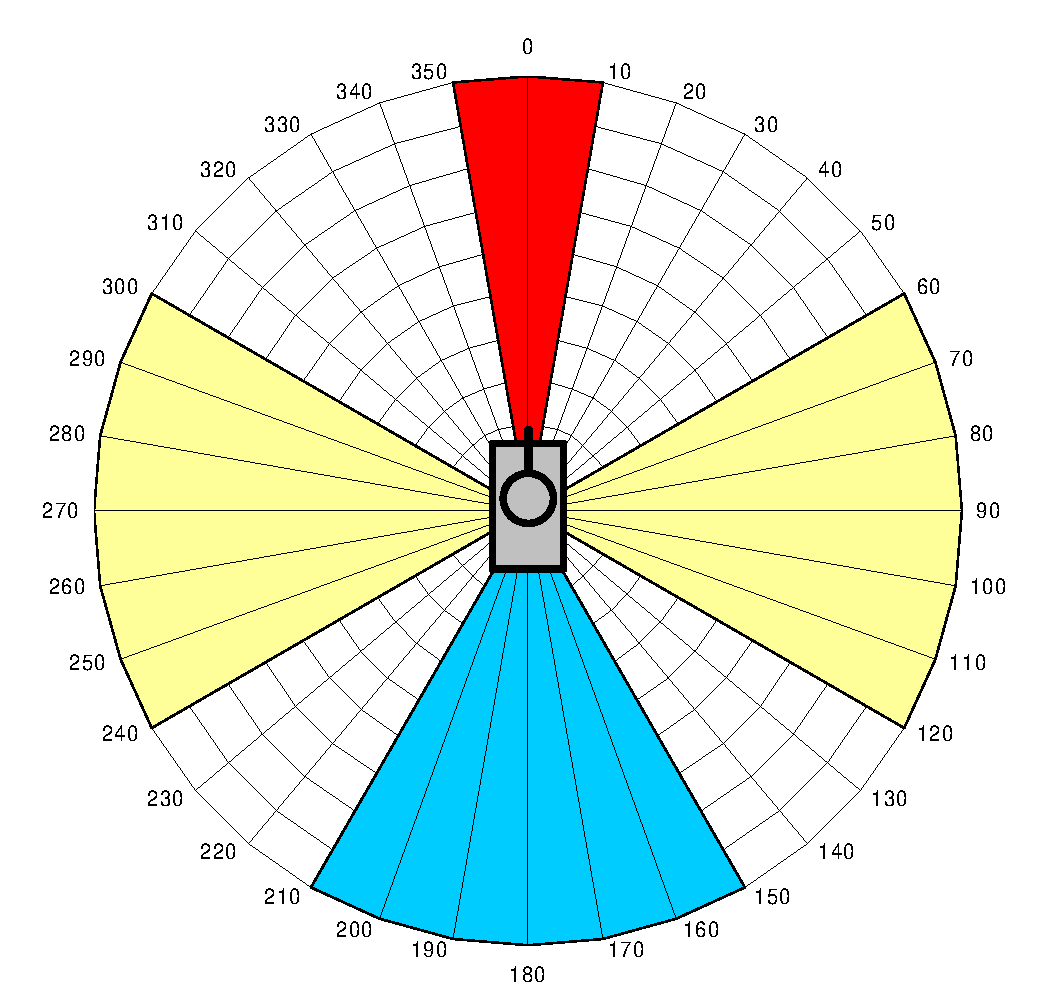
\includegraphics[width=.6\textwidth]{zones}}
%        \put(5.05,1.7){\squareciws}
%        \put(5.05,1.3){\squaregun}
%        \put(5.05,0.9){\squarestir}
        \put(6,3){
                \begin{tabular}{|p{.32\textwidth}|l}
                    \cline{1-1}
                \centering \textbf{�tat de Base} \\ 1 STIR, 1 Gun,\\ 1 CIWS, 2 MLs & ~\\
                    \cline{1-1}
                \cellcolor[rgb]{0.941,0.22,0.231}\centering \textbf{Pas de CIWS} & ~\\
                    \cline{1-1}
                \cellcolor[rgb]{0.322,0.753,0.945}\centering  \textbf{Pas de Gun} & ~\\
                    \cline{1-1}
                \cellcolor[rgb]{0.996,1,0.627}\centering  \textbf{Un STIR additionnel} & ~ \\
                    \cline{1-1}
                \end{tabular}
        }
        \end{picture}
\centering \caption[NEREUS: Exemples d'angles morts]{\label{tab:blind}Angles morts: Le Gun et le \textsc{ciws} �tant plac� respectivement � l'avant et � l'arri�re du navire, il ne peuvent pas tirer au travers de celui-ci. Les deux stirs sont eux aussi orient� l'un vers l'avant, l'autre vers l'arri�re, permettant ainsi que les deux soient disponibles sur chacun des flancs du b�timent.}
\end{table}

\begin{table}[!htb]
\renewcommand\arraystretch{1.2}% (1.0 is for standard spacing)
    \begin{tabular}{|l|l|c|}
            \hline
        Arme & Port�e & Probabilit� de succ�s  \\
            \hline
        ML & From 2.2 to 20km &95\% \\
            \hline
        Gun & From 1.5 to 5km  &50\% \\
            \hline
        CIWS& From 0.2 to 2km  &30\%  \\
            \hline
   \end{tabular}
   \vspace{5pt}
\centering \caption[NEREUS: Exemples de r�sultats des actions]{\label{tab:pk}R�sultats des actions: Cette table sp�cifie la port�e des diff�rentes armes et les probabilit�s que chacune d'elle r�ussisse � d�truire la menace qui lui aurait �t� allou�e.}
\end{table}

Un probl�me statique d'allocation d'armes repr�sent� sous forme de \textsc{csp} tel que pr�sent� figure~\ref{fig:wtacsp} peut-�tre formalis� de la mani�re suivante:
\begin{itemize}
    \item $X = \mathcal{W} $ ensemble des $w$ ressources du probl�me ;
    \item $D = \mathcal{M} $ ensemble des $m+1$ t�ches associ�es aux ressources (i.e., leurs allocations possibles � un instant donn�) plus la possibilit� de ne rien faire ;
    \item $C = \{c_1 , ... , c_k , ... c_n\}$ ensemble des $n$ contraintes, sp�cifiant les combinaisons de t�ches mutuellement compatibles.
\end{itemize}
L'objectif �tant de trouver une allocation possible des t�ches aux ressources suivant les contraintes entre les ressources.

\begin{figure}[!hbt]
\begin{center}
        \begin{tikzpicture}[scale=2]%
        \begin{scope}
            \tikzstyle{every node}=[draw,circle,fill=blue!1!white,minimum size=1.2cm];%%
            \node (w1) at (0,0)  {$\omega_1$}; %%
            \node (w2) at (-1,1)  {$\omega_2$}; %%
            \node (w3) at (-.35,2)  {$\omega_3$}; %%
            \node (wj) at (.8,2.2)  {$\omega_j$}; %%
            \node (wwm1) at (2,1.2)  {$\omega_{w-1}$}; %%
            \node (ww) at (1.3,0)  {$\omega_w$}; %%
        \end{scope}
        \begin{scope}
    \tikzstyle{every node}=[draw,fill=blue!20!white,font=\footnotesize];%%
    \node[left=15pt,below] (d1) at (w1.west)  {\begin{tabular}{c}$\mathcal{D}_1$:\\$T_1$\\$T_2$\\...\\$T_i$\\...\\$T_m$\end{tabular}}; %%
    \node[left=15pt,below] (d2) at (w2.west)  {\begin{tabular}{c}$\mathcal{D}_2$:\\$T_1$\\$T_2$\\...\\$T_i$\\...\\$T_m$\end{tabular}}; %%
    \node[left=15pt,above] (d3) at (w3.west)  {\begin{tabular}{c}$\mathcal{D}_3$:\\$T_1$\\$T_2$\\...\\$T_i$\\...\\$T_m$\end{tabular}}; %%
    \node[right=15pt,above] (dj) at (wj.east)  {\begin{tabular}{c}$\mathcal{D}_j$:\\$T_1$\\$T_2$\\...\\$T_i$\\...\\$T_m$\end{tabular}}; %%
    \node[right=1pt] (dwm1) at (wwm1.east)  {\begin{tabular}{c}$\mathcal{D}_{w-1}$:\\$T_1$\\$T_2$\\...\\$T_i$\\...\\$T_m$\end{tabular}}; %%
    \node[right=15pt,below] (dw) at (ww.east)  {\begin{tabular}{c}$\mathcal{D}_w$:\\$T_1$\\$T_2$\\...\\$T_i$\\...\\$T_m$\end{tabular}}; %%
        \end{scope}
        \draw (w1)--(w2); %%
        \draw (w1)--(ww); %%
        \draw (w2)--(w3); %%
        \draw (w2)--(wwm1); %%
        \draw[dashed] (w1)--(wj); %%
        \draw[dashed] (w3)--(wj); %%
        \draw[dashed] (wwm1)--(wj); %%
        \draw[dashed] (ww)--(wj); %%
        \draw (wwm1)--(ww); %%
        \end{tikzpicture}%
    \caption[Mod�lisation \textsc{csp} du \emph{Weapon-Target Assignment}.]{\label{fig:wtacsp} Mod�lisation \textsc{csp} du \emph{Weapon-Target Assignment} o� les armes sont les variables et les t�ches repr�sentent le domaine. Voir le texte pour plus de d�tails.}
\end{center}
\end{figure}

Il est cependant possible d'avoir des contraintes temporelles entre les t�ches plut�t que des contraintes entre les ressources. Dans ce cas
pr�cis, on pr�f�rera employer la formulation ci-dessous, duale de celle exprim�e pr�c�demment:
\begin{itemize}
    \item $X = \mathcal{M} $ ensemble des $m$ t�ches du probl�me ;
    \item $D = \mathcal{W} $ ensemble des $w$ ressources associ�s aux t�ches (i.e., leurs allocations possibles � un instant donn�) ;
    \item $C = \{c_1 , ... , c_k , ... c_n\}$ ensemble des $n$ contraintes, sp�cifiant les combinaisons de ressources mutuellement compatibles.
\end{itemize}
L'objectif �tant de trouver une allocation possible des ressources aux t�ches suivant les contraintes entre les t�ches.

\subsection{Utilisation des contraintes seules}

Dans notre probl�me, nous avons choisi d'impl�menter l'instance du probl�me pr�c�demment �voqu� en sp�cifiant le \textsc{m}a\textsc{csp} de la mani�re suivante: Les variables de d�cision sont les armes dont les domaines sont les menaces (on doit assigner � chaque arme une menace). Les contraintes et les probabilit�s de transition sont sp�cifi�es telles qu'indiqu�es dans les tables \ref{tab:constraints}, \ref{tab:blind} et \ref{tab:pk}. Les menaces apparaissent � des distances distribu�es selon une gaussienne autour de 20 km de la plate-forme et selon un azimut distribu� uniform�ment autour de la plate-forme. On suppose que l'�tat des menaces (distance, azimut) �volue de mani�re d�terministe. Ainsi, on conna�t pr�cis�ment quelle va �tre l'�volution des contraintes au cours du temps. La Figure \ref{fig:CSP} montre le \textsc{dcsp} � l'�tat initial et comment il peut �voluer durant un �pisode. Il existe des contraintes unaires qui sp�cifient quelles sont les menaces ``visibles'' par les armes selon leur distance et leur azimut, et des contraintes binaires qui associent des radars � des armes pour pouvoir tirer ou sp�cifient certaines impossibilit�s. Dans cet exemple, les contraintes �voluent � chaque changement d'�tat, ou r�solution d'engagement, � savoir si une arme a atteint une cible ou non. Les contraintes sont alors modifi�es dynamiquement pour refl�ter l'utilisation actuelle des radars et des armes.

\begin{figure}[!htb]
\begin{center}
        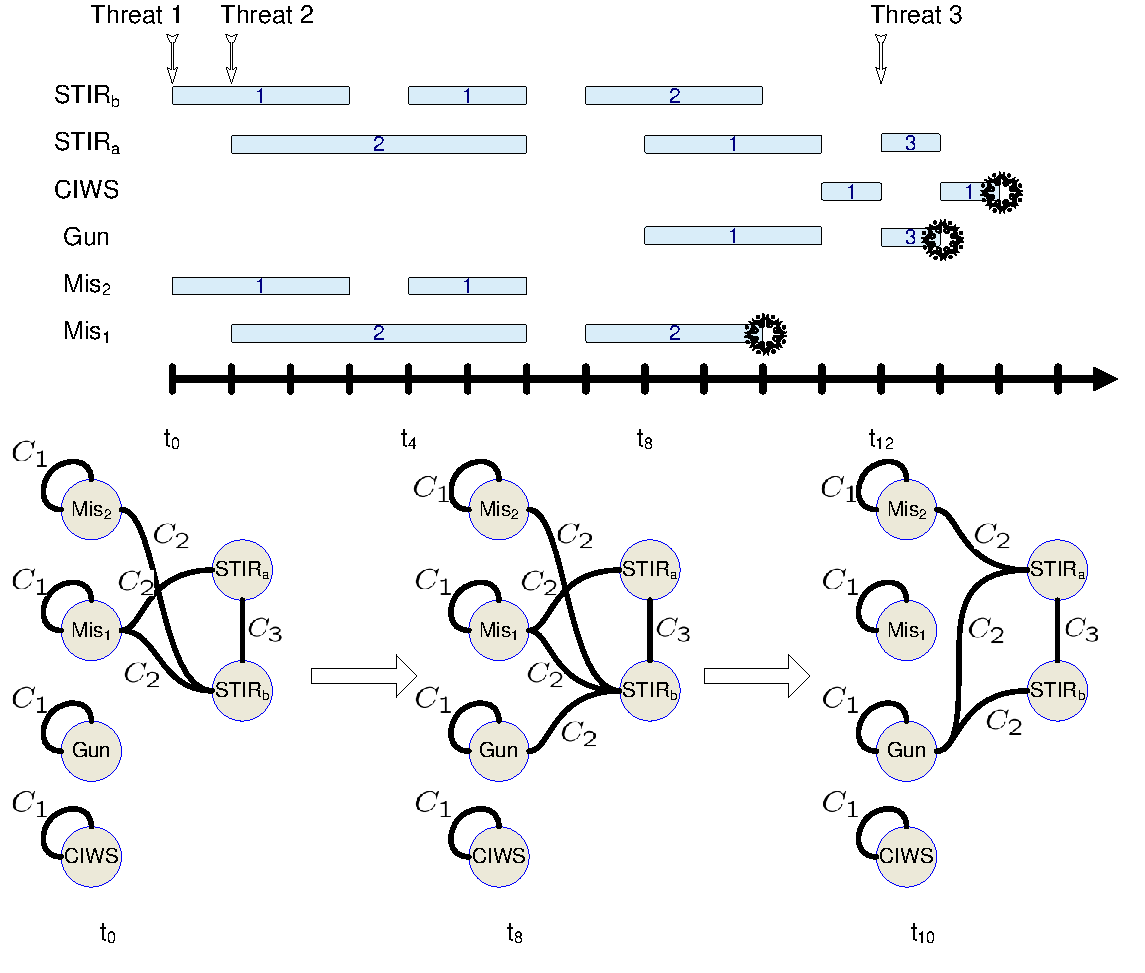
\includegraphics[width=.8\textwidth]{timeline_MaCSP}
\end{center}
\caption{\label{fig:CSP}Exemple de plan (en haut) et d'�volution du \textsc{dcsp} associ� (en bas) pendant un �pisode.}
\end{figure}

\begin{figure}[!htb]
\begin{center}
\subfigure[Time (ms) vs \# Tasks\label{fig:time}]{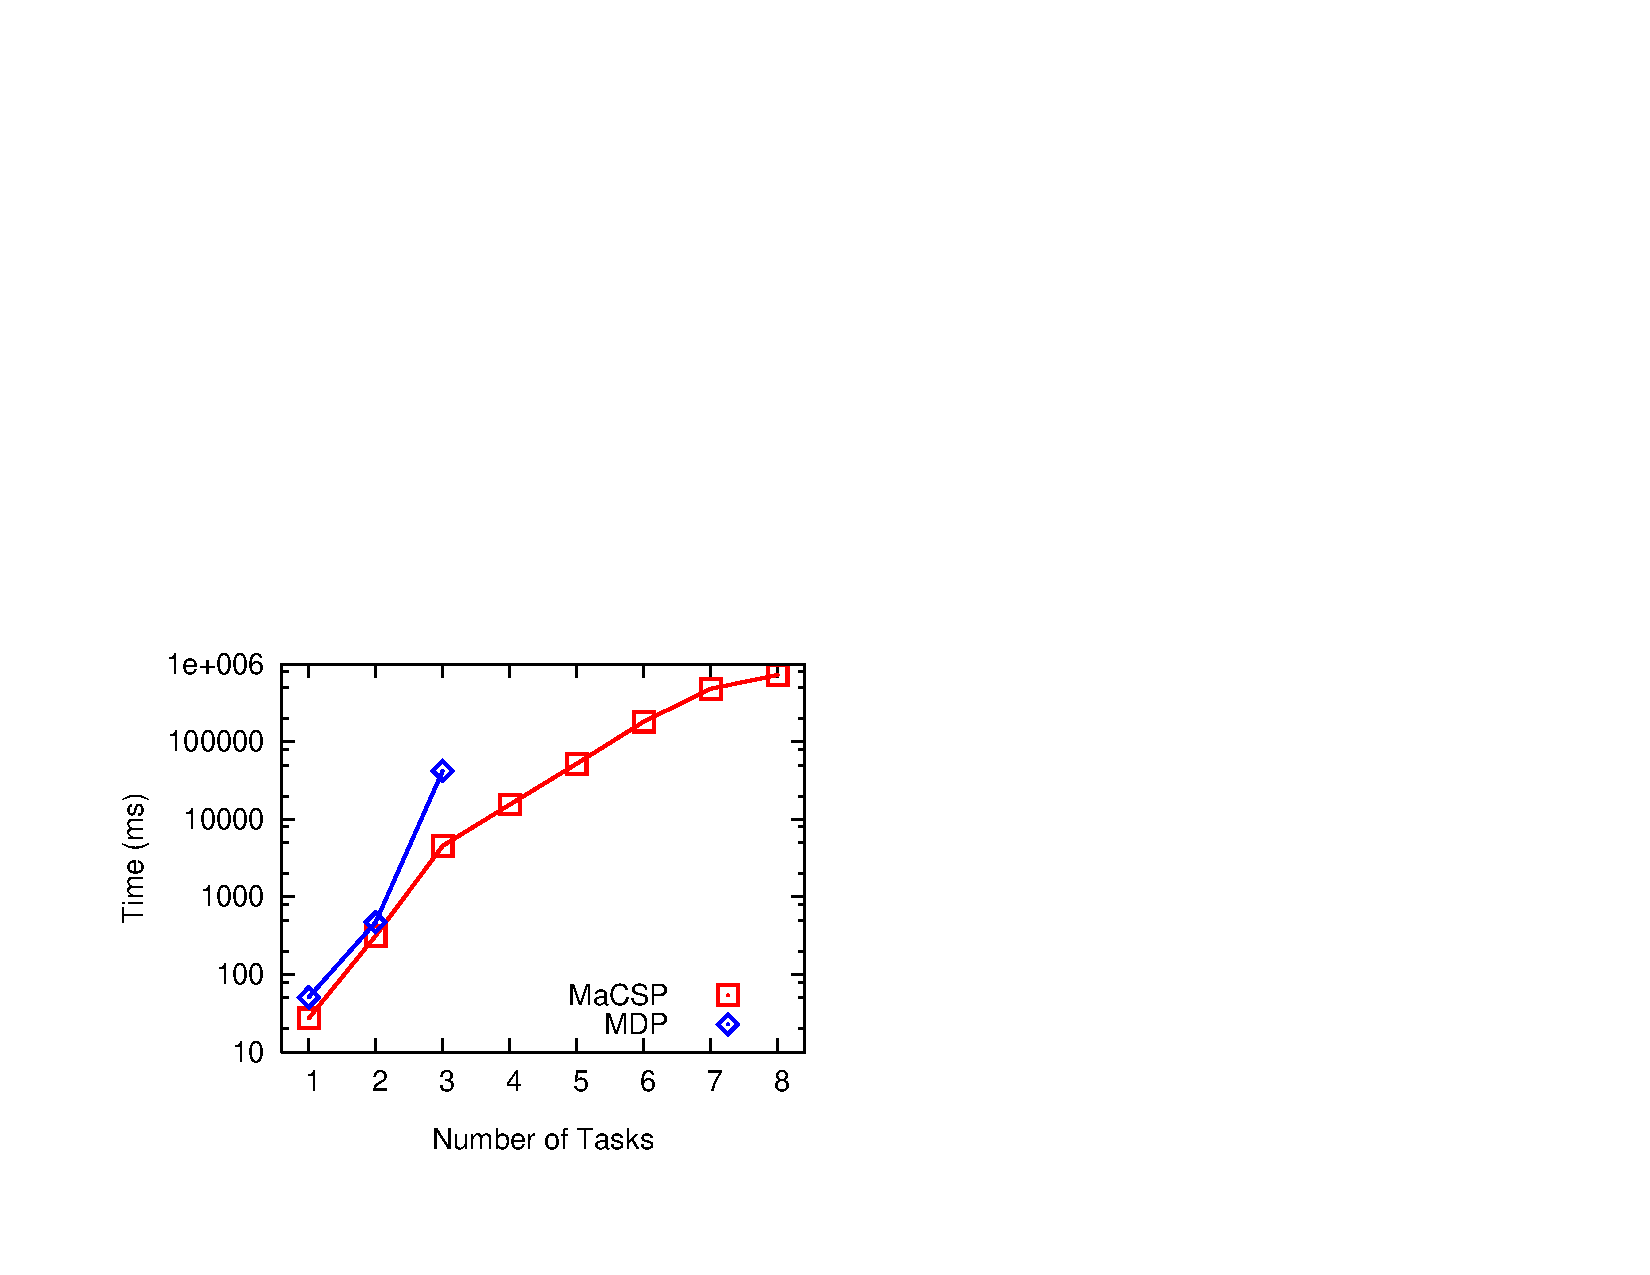
\includegraphics[width=.48\textwidth]{MaCSPvsMDP_time}}%%
%\end{center}
%~\\
%\begin{center}
\subfigure[\# Backups vs \# Tasks\label{fig:back}]{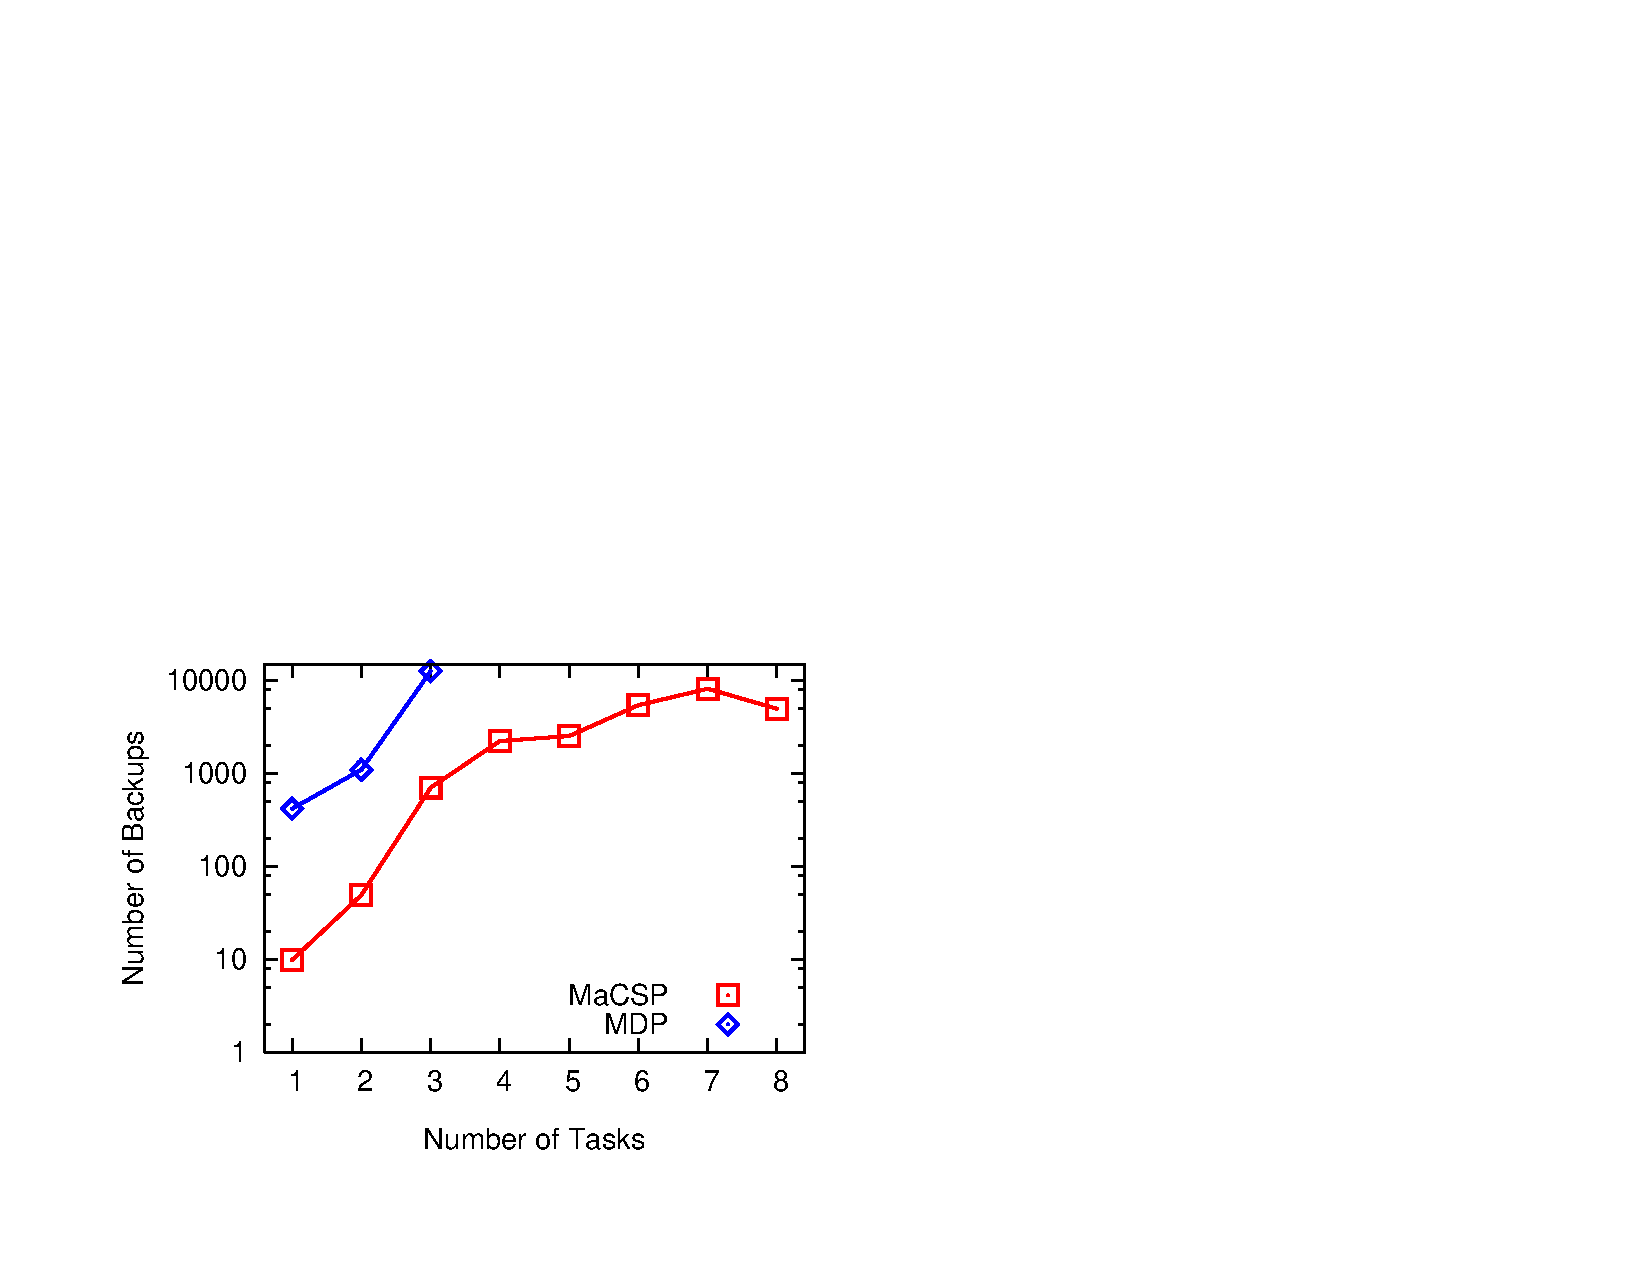
\includegraphics[width=.48\textwidth]{MaCSPvsMDP_backups}}
\end{center}
\caption{\label{fig:res}Comparaison entre \mdp et \macsp.}
\end{figure}

Nous avons compar� notre mod�le avec un \mdp factoris� sans contrainte, mais en donnant des probabilit�s nulles de succ�s lorsqu'une assignation �tait interdite (par exemple un missile tir� sur une menace trop �loign�e a une chance nulle de l'atteindre). Les r�sultats pr�sent�s en Figure \ref{fig:res} sont obtenus en utilisant le \textsc{frtdp} classique pour le \mdp et notre adaptation pour le \textsc{m}a\textsc{csp}. Chaque point est une moyenne sur 300 simulations. Nous avons utilis� pour ces tests les ``pires bornes possibles'': une borne inf�rieure nulle et une borne sup�rieure comme si les assignations d'armes faisables �taient toujours un succ�s. Ces bornes ont �t� utilis�es pour v�rifier la r�elle efficacit� de l'algorithme sans aucun b�n�fice tir� des bornes utilis�es. Les r�sultats de la figure \ref{fig:time} repr�sentent le temps de calcul pour la planification optimale tandis que la figure \ref{fig:back} repr�sente le nombre de mises � jour de Bellman (appel � la fonction \textsc{backup} de l'algorithme \ref{alg:FRTDP}) en fonction du nombre de t�ches. On pouvait s'attendre � ce genre de r�sultats pour les \mdps puisque la taille de l'espace d'�tat cro�t exponentiellement suivant le nombre de t�ches et de ressources. On voit cependant qu'on gagne un ordre de magnitude en restreignant l'espace de recherche par les contraintes.

\subsection{Utilisation des contraintes dans une borne}

Nous avons �galement adapt� les bornes initialement propos�es par \cite{PCB.07} pour am�liorer les performances de l'algorithme. La borne sup�rieure n'a pas �t� modifi�e et utilise la m�me factorisation en t�che pour am�liorer le temps d'�valuation de la borne. En revanche, la borne inf�rieure se base sur la r�solution par contraintes et sur un algorithme r�actif r�alisant la t�che la plus urgente pour obtenir une bien meilleure estimation de la fonction de valeur minimum � un co�t de calcul tr�s l�g�rement sup�rieur. Ainsi, les gains r�alis�s en temps de calcul sont plus cons�quent dus � un meilleur �lagage de l'arbre de recherche. Les r�sultats sont rapport�s dans la figure~\ref{fig:cspBound}

\begin{figure}[!htb]
\begin{center}
        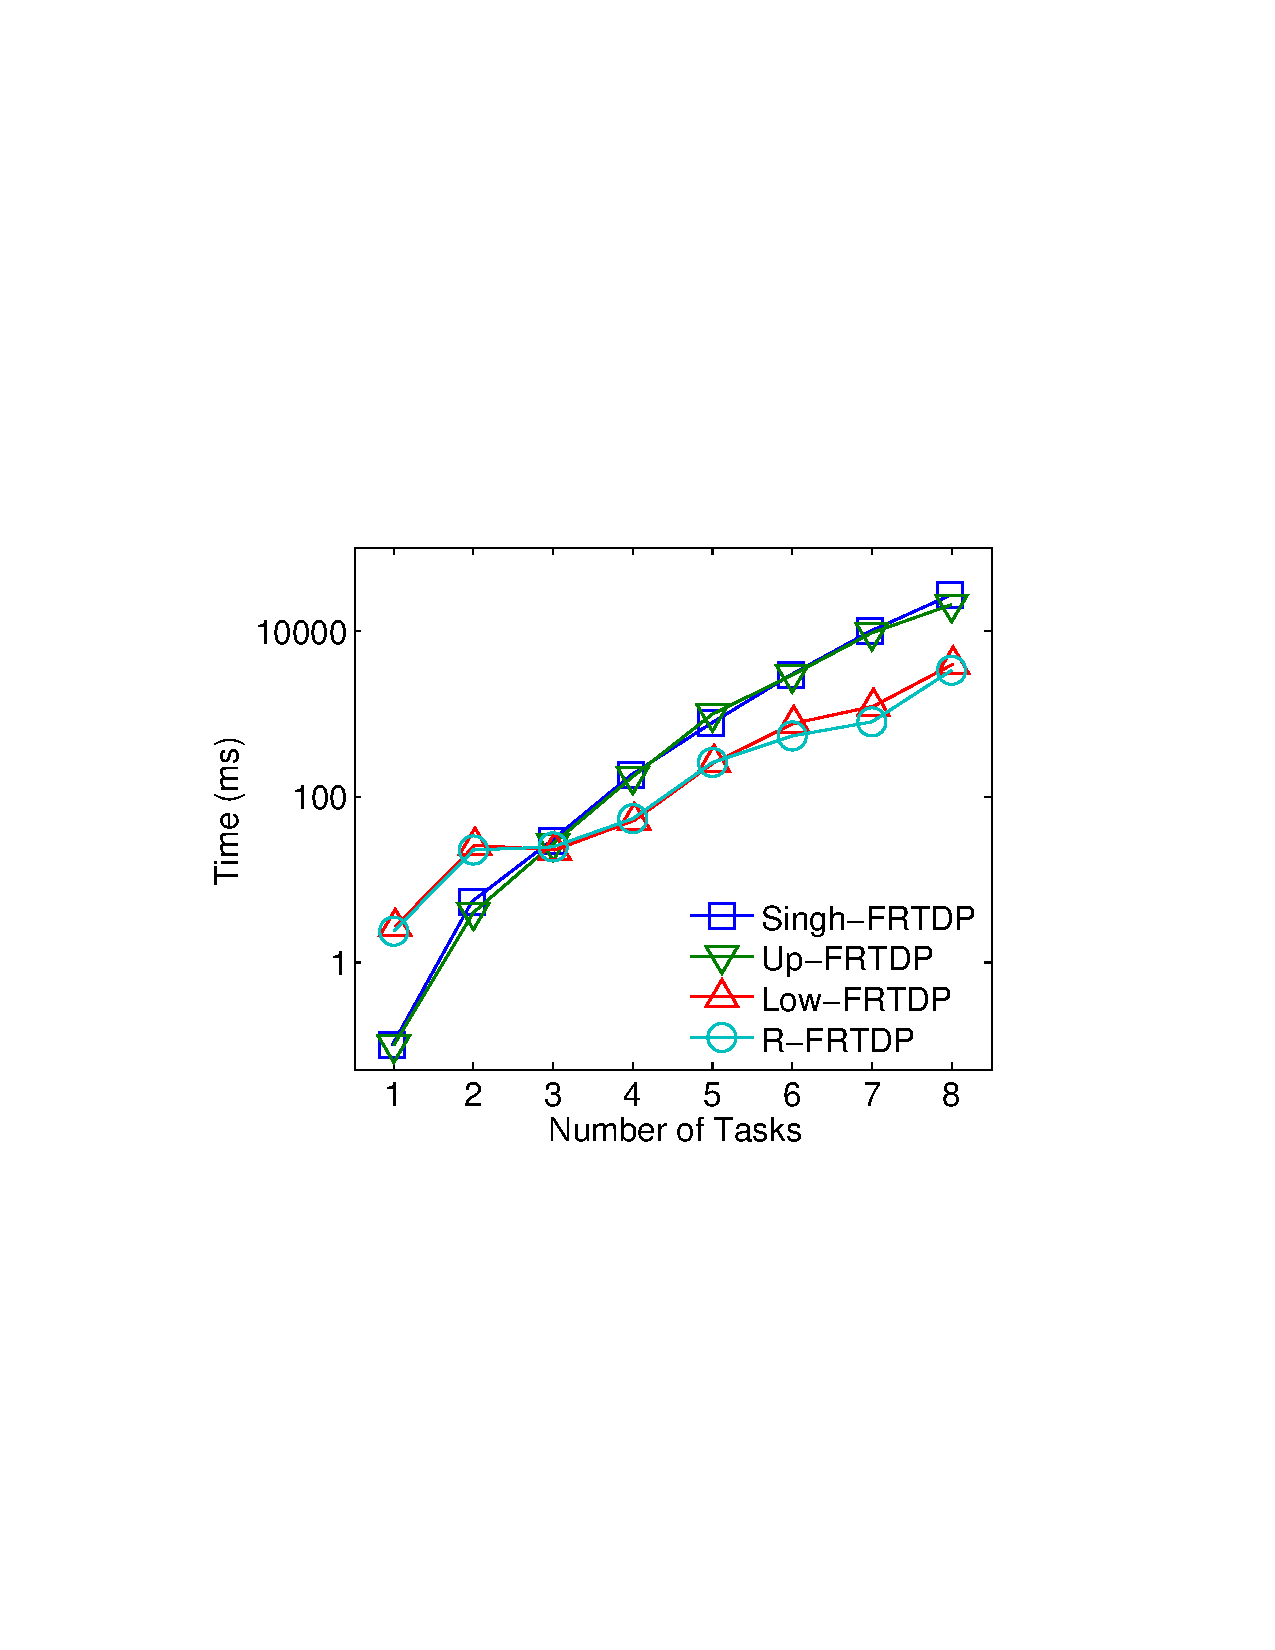
\includegraphics[width=.5\textwidth]{results}
\end{center}
\caption{\label{fig:cspBound}Comparaison de l'utilisation de borne � base de \textsc{csp} versus les bornes de la litt�rature.}
\end{figure}

Pour ces r�sultats, nous avons compar� l'utilisation des contraintes dans la borne inf�rieure versus les bornes disponibles dans la litt�rature. Singh-\textsc{frtdp} repr�sente l'algorithme de base \textsc{frtdp} utilisant les bornes propos�es par \cite{SC.98}. Up-\textsc{frtdp} est l'algorithme \textsc{frtdp} utilisant la borne sup�rieure de \cite{PCB.07} et la borne inf�rieure de \cite{SC.98}. Low-\textsc{frtdp} utilise la borne sup�rieure de \cite{SC.98} et la borne inf�rieure � base de contraintes. R-\textsc{frtdp} utilise la borne sup�rieure de \cite{PCB.07} et la borne inf�rieure � base de contraintes.

Les r�sultats indiquent clairement que les contraintes ne deviennent int�ressantes � utiliser que lorsque le nombre de t�ches devient important (ici sup�rieur � 3) mais que le gain s'av�re finalement substantiel lorsque le nombre de t�ches continue � cro�tre (la figure utilise une �chelle logarithmique sur les ordonn�es).

\section{Conclusion}

Ce chapitre a, tout d'abord, fait �tat du probl�me d'allocation d'armes � des cibles tel que pr�sent� dans la litt�rature. La version statique de ce probl�me a premi�rement �t� d�taill�e avant de pr�senter la version dynamique et les diff�rentes versions sous incertitudes. Un aper�u des mod�les de satisfaction de contraintes a �galement �t� introduit comme introduction au mod�le de Markov propos� dans ce chapitre. Un analyse th�orique a �t� r�alis�e montrant que la complexit� \emph{en pire cas} n'est pas favorable au d�veloppement de tels mod�les. Cependant, les exp�rimentations ont montr� que, vu que le nombre de variables d'�tat est tr�s souvent tr�s inf�rieur (selon une loi logarithmique) au nombre d'�tats rencontr�s, l'approche propos�e permet des r�ductions substantielles du temps de calcul dans le probl�me d'allocation de ressources.

Parmi les travaux futurs envisag�s � la suite de ce projet, plusieurs avenues de recherche ont attir� notre attention. Premi�rement, l'hypoth�se est faite que les perceptions de l'agent sont parfaites et donc que l'�tat du syst�me est enti�rement observ� � chaque instant de d�cision. De fait, dans la r�alit�, les radars de navires sont rarement parfaits et un certaine incertitude est pr�sente sur la position de menaces, sur les temps de vol des missiles et sur les observations de r�ussites (ou non) des contre-mesures. Il �tait donc naturel de regarder du c�t� des processus de Markov partiellement observables pour continuer nos travaux. D'autre part, nous avons consid�r� dans ce chapitre qu'un seul b�timent avait � faire face � une attaque ennemie. En pratique, aucun navire ne circule seul et c'est souvent une flottille qui est sous l'effet d'une attaque ennemie.  Il a donc �t� envisag� d'�tudier les comportements d'un ensemble de navires sous les conditions pr�c�demment �voqu�es.

Malheureusement, comme nous le verrons au chapitre suivant, la complexit� des mod�les de Markov multiagents partiellement observables est telle qu'aucun mod�le actuel n'est en mesure de proposer une solution efficace pour le probl�me consid�r�. Nous allons donc vous d�tailler dans les chapitres suivants comment nous pensons qu'il est n�cessaire de mod�liser ce type de probl�me pour le rendre resolvable, et ce, m�me lorsque plusieurs agents doivent agir dans un environnement hostile et incertain.

%\begin{note}
%Mettre les algorithmes de r�solution de \textsc{csp} par Forward Checking et par �limination de variable ?
%\end{note}

\newpage\phantom{a}

%\part{Contraintes sur l'observation}

% Bornes Observabilit�
\chapter{Contraintes sur l'observabilit� des processus de Markov}

% \emph{�Ce qui est important c'est l'esprit d'�quipe. Les mecs, y sont une �quipe, y'a un esprit, alors forcement, il faut qu'ils partagent.�}
% \begin{flushright} Coluche \end{flushright}
% \bigskip
% \emph{�Observer est le plus durable des plaisirs de la vie.�}
% \begin{flushright} Diane � la crois�e des chemins -- Georges Meredith \end{flushright}
% \bigskip
 \emph{�L'important, c'est de savoir ce qu'il faut observer.�}
 \begin{flushright} Histoires Extraordinaires -- Edgar Allan Poe \end{flushright}
 \bigskip

\begin{summary}
Ce chapitre introduit tout d'abord la probl�matique de la complexit� associ�e � l'observabilit� partielle dans les processus d�cisionnels de Markov. Il d�bute par un aper�u de la complexit� des diff�rents mod�les existants et introduit ensuite un nouveau type d'observabilit� contrainte par le concepteur. Ce nouveau type d'observabilit�, qualifi� de \emph{bijectivement observable} permet, dans certain cas identifi�s, de r�aliser des gains substantiels en complexit� en pire cas. Ce chapitre d�taille donc les apports pour le mod�le � un seul agent partiellement observable (\pomdp) avant d'�tendre au mod�le � plusieurs agents (\decpomdp). Des exemples d'applications sont ensuite mod�lis�s et pr�sent�s.
\end{summary}

\label{chap:4}

\section{Introduction}

La disponibilit� et la compl�tude de l'information ont toujours �t� des facteurs pr�pond�rant dans le domaine de la prise de d�cision. Dans les processus d�cisionnels de Markov, o� toute l'information n�cessaire est rassembl�e dans l'�tat du syst�me, l'observabilit� de cet �tat influence �norm�ment la complexit� de la prise de d�cision dans cet �tat. Toutefois, il est tr�s rare de trouver des cas ou l'information disponible est parfaite et compl�te � la fois.

Introduite par~\cite{D.62}, l'observabilit� partielle mod�lise cet aspect incomplet ou bruit� de l'observation de l'�tat par l'agent intelligent. Une \emph{fonction d'observation} est alors utilis�e qui associe � chaque �tat une distribution sur un ensemble restreint de symboles. Une autre mani�re de voir cette observabilit� partielle est de consid�rer que l'�tat est transmis au travers d'un canal de communication bruit� (e.g. les capteurs). Cette repr�sentation tr�s g�n�rale permet de mod�liser tous les niveaux d'observabilit�, depuis l'observabilit� compl�te, o� � chaque �tat est associ� un symbole particulier qui peut �tre l'�tat lui-m�me, jusqu'� l'observabilit� nulle, o� � chaque �tat est associ� le m�me symbole. Cette repr�sentation � �t� utilis�e dans tous les mod�les de Markov depuis, et en particulier dans les \pomdps pour le cas � un seul agent, et dans les \decpomdps dans le cas multiagent.

Cependant, avec l'observabilit� partielle vient n�cessairement une augmentation de la complexit� algorithmique en pire cas. Comme d�montr� dans la figure~\ref{fig:compObs}, � mesure que l'observabilit� diminue, i.e. que les agents ont de moins en moins d'information pour raisonner, la complexit� augmente g�n�ralement.

\begin{figure}[h!tb]
\begin{center}
    \begin{tikzpicture}[line width=.1ex, scale=1]
        %\draw[step=0.1cm,color=gray,very thin] (-2,-2) grid (11,11);%%
        \begin{scope}[font=\footnotesize]
        \node[below] at (8.5,0) {Partielle};  %%
        \node[below=10pt] at (8.5,0) {\& Imparfaite};  %%
        \node[below=] at (6,0) {Conjointe};  %%
        \node[below=10pt] at (6,0) {\& Parfaite};  %%
        \node[below] at (3.5,0) {Compl�te};  %%
        \node[below=10pt] at (3.5,0) {\& Imparfaite};  %%
        \node[below] at (1,0) {Compl�te};  %%
        \node[below=10pt] at (1,0) {\& Parfaite};  %%
        \node[below] at (10,0) {Nulle};  %%
        \end{scope}
%        \node[align=right,anchor=east] at (0,8.5) {\textsc{nexp}};  %%
%        \node[align=right,anchor=east] at (0,7.5) {\textsc{exp}};  %%
%        \node[align=right,anchor=east] at (0,7) {\textsc{pspace}};  %%
%        \node[align=right,anchor=east] at (0,2) {\textsc{np}};  %%
%        \node[align=right,anchor=east] at (0,1) {\textsc{p}};  %%
        \node[anchor=east] at (0,8.5) {\textsc{nexp}};  %%
        \node[anchor=east] at (0,7.5) {\textsc{exp}};  %%
        \node[anchor=east] at (0,7) {\textsc{pspace}};  %%
        \node[anchor=east] at (0,2) {\textsc{np}};  %%
        \node[anchor=east] at (0,1) {\textsc{p}};  %%
        \node at (5,4.5) {\LARGE{Foss�}};%%
        \draw[thin] (0,8.5) -- (8.5,8.5); \draw[thin,dashed] (8.5,8.5) -- (10,8.5);
        \draw[thin] (0,7) -- (8.5,7); \draw[thin,dashed] (8.5,7) -- (10,7);
        \draw[thin] (0,2) -- (8.5,2); \draw[thin,dashed] (8.5,2) -- (10,2);
        \draw[thin] (0,1) -- (8.5,1); \draw[thin,dashed] (8.5,1) -- (10,1);
        \draw[thin,dashed,draw=gray] (10,0) -- (10,8.5);
        \draw[thin,dashed,draw=gray] (8.5,0) -- (8.5,8.5);
        \draw[thin,dashed,draw=gray] (6,0) -- (6,8.5);
        \draw[thin,dashed,draw=gray] (3.5,0) -- (3.5,8.5);
        \draw[thin,dashed,draw=gray] (1,0) -- (1,8.5);
        \pgfsetfillopacity{0.5}
        \shade [right color=white,left color=blue!50!white] (0,2.1) rectangle (11,6.9);
        \pgfsetfillopacity{1.0}
        \draw[->,-latex,line width=.5ex,red] (-.05,0) -- (11,0) node[anchor=south]{Observabilit�};  %%
        \draw[->,-latex,line width=.5ex,red] (0,-.05) -- (0,10) node[anchor=west]{Complexit�};  %%
        \filldraw (1,1) circle (2pt) node[anchor=250]{(\textsc{m})\textsc{mdp}$_\infty$};%%
        \filldraw (10,2) circle (2pt) node[anchor=south]{\textsc{u}\mdp};%%
        \filldraw (10,7) circle (2pt) node[anchor=south]{\textsc{umdp}$_\infty$};%%
        \filldraw (3.5,7) circle (2pt) node[anchor=south]{(\textsc{m})\pomdp};%%
        \filldraw (6,8.5) circle (2pt) node[anchor=north]{\decmdp};%%
        \filldraw (6,1) circle (2pt) node[anchor=south]{Free Com.};%%
        \filldraw (6,1) circle (2pt) node[anchor=north]{\decmdpcom};%%
        \filldraw (8.5,8.5) circle (2pt) node[anchor=south]{\decpomdp};%%
        \filldraw (8.5,7) circle (2pt) node[anchor=340]{Free Com.};%%
        \filldraw (8.5,7) circle (2pt) node[anchor=20]{\decpomdpcom};%%
    \end{tikzpicture}  \caption{Mesure de la complexit� fonction de l'observabilit�}\label{fig:compObs}
\end{center}
\end{figure}
Ainsi, en pr�sence d'information compl�te et parfaite -- lorsque le ou les agents ont enti�rement acc�s � l'�tat r�el du syst�me -- le probl�me � r�soudre est seulement \textsc{p}-complet. Seulement, d�s que l'observation devient imparfaite, et m�me si elle reste compl�te -- lorsque tous les agents ont la m�me information bruit�e de l'�tat du syst�me -- r�soudre le probl�me devient alors \textsc{pspace}-complet, et ce, m�me si la fonction de transition est d�terministe (c.f. les \pomdps d�terministes ou \textsc{d}et\pomdps au chapitre 6 de la th�se de~\cite{L.96}). La d�centralisation de l'information -- lorsque les agents n'ont plus n�cessairement acc�s � la m�me information bruit�e sur l'�tat du monde -- accro�t encore cette complexit� du probl�me jusqu'� la \textsc{nexp}-compl�tude. Les cas particuliers du \decmdpcom avec communications gratuites et du \textsc{u}\mdp (Unobservable \mdp) sont facilement explicables. Dans le cas du \decmdpcom, les agents ont une vue non bruit�e locale du syst�me. Ainsi, de par la communication, ils peuvent s'�changer toutes leurs vues locales pour obtenir une vue globale �quivalente au probl�me o� chacun aurait d�j� cette observabilit� compl�te en partant. Dans le cas du \mdp non observable, le cas est simple puisque ne sachant pas o� ils se trouvent, les agents ne raisonnent plus sur les �tats possibles du monde, mais seulement sur les objectifs � atteindre et sur leur probabilit� de r�alisation.

Il convient toutefois de remarquer, comme le montre la figure~\ref{fig:compObs}, qu'il existe un foss� extr�me lorsque l'on passe du cas compl�tement observable (ou non observable), au cas partiellement observable. Ceci s'explique en partie par la tr�s grande capacit� de repr�sentation des mod�les partiellement observables, leur conf�rant une expressivit� � la mesure de leur complexit�. Dans les sections suivantes, les travaux r�alis�s cherchent donc � r�duire cette complexit� tout en �quilibrant au mieux l'expressivit�. Des mod�les particuliers d'observabilit� ont �t� d�velopp�s � cette fin permettant ainsi de r�duire cette complexit� tout en gardant une expressivit� suffisante.

Pour r�duire une telle complexit�, nous avons tout d'abord convenu de restreindre notre �tude aux mod�les monoagents � transition d�terministe. La version multiagent sera ensuite pr�sent�e avant de discuter de l'extension possible au cas stochastique de la fonction de transition. Rappelons donc tout d'abord les processus de Markov partiellement observables d�terministes avant de proposer de nouveaux mod�les d'observation.

\section{\pac{pomdp}s quasi-d�terministes}\label{sect:qdetpomdp}

Les \pomdps d�terministes ont �t� d�finis par~\cite{L.96}, comme suit:
\begin{definition}\label{def:detpomdp}
Un Processus D�cisionnel de Markov Partiellement Observable D�terministe (\detpomdp) est un tuple $\la \Sta,$ $\Act,$ $\Omega,$ $\Tra,$ $\Obs,$ $\Rew,$ $\gamma,$ $\bel^0 \ra$, o�:%\\
\begin{itemize}
\item $\Sta$ est un ensemble fini d'\emph{�tats} $s \in \Sta$;
\item $\Act$ est un ensemble fini d'\emph{actions} $a \in \Act$;
\item$\Tra(s,a,s'): \Sta \times \Act \times \Sta \mapsto \{0,1\}$ est la \emph{fonction d�terministe de transition} du syst�me de l'�tat $s$ vers l'�tat $s'$ apr�s l'ex�cution de l'action $a$;
\item $\Rew(s,a): \Sta \times \Act \mapsto \mathds{R}$ est la \emph{r�compense} produite par le syst�me lorsque l'action $a$ est ex�cut�e dans l'�tat $s$,
\item $\Omega$ est un ensemble fini d'observations $o \in \Omega$,
\item $\Obs(s,a,o,s'): \Sta \times \Act \times \Omega \times\Sta \mapsto \{0,1\}$ est la \emph{fonction d�terministe} qui indique si l'observation $o$ survient ou non lors de la transition du syst�me de l'�tat $s$ vers l'�tat $s'$ sous l'effet de l'action $a$.
\item $\gamma$ est le facteur d'escompte;
\item $\bel^0$ est la connaissance \emph{a priori} sur l'�tat, i.e. l'�tat de croyance initial, suppos� non d�terministe.
\end{itemize}
\end{definition}

Remarquons que l'�tat de croyance initial $\bel^0$ -- qui d�crit les diff�rentes possibilit�s pour l'�tat de d�part -- est crucial. En effet, si l'�tat de d�part est connu, et la transition d'un �tat vers un autre d�terministe, alors la s�quence compl�te des �tats suivants est �galement pr�visible, et le probl�me de \detpomdp se ram�ne alors au probl�me d�j� tr�s �tudi� dans la litt�rature de l'IA de la planification d�terministe~\citep{GNT.04}.

\hyphenation{qua-si-d\'e-ter-mi-ni-ste}
Par comparaison au \pomdp d�terministe, l'extension que nous proposons modifie la d�finition de la fonction d'observation de telle sorte qu'elle soit maintenant stochastique tout en assurant qu'il existe certaines observations qui sont vraiment plus probables que d'autres dans chacun des �tats. Formellement:
\begin{definition}\label{def:qdetpomdp}
Un processus d�cisionnel de Markov partiellement observable quasi-d�terministe (\qdetpomdp) est un tuple $\la \Sta,$ $\Act,$ $\Tra,$ $\Obs,$ $\Rew,$ $\gamma,$ $\bel^0 \ra$, o� :
\begin{itemize}
\item $\Sta$ est un ensemble fini d'\emph{�tats} $s \in \Sta$;
\item $\Act$ est un ensemble fini d'\emph{actions} $a \in \Act$;
\item$\Tra(s,a,s'): \Sta \times \Act \times \Sta \mapsto \{0,1\}$ est la \emph{fonction d�terministe de transition} du syst�me de l'�tat $s$ vers l'�tat $s'$ apr�s l'ex�cution de l'action $a$;
\item $\Rew(s,a): \Sta \times \Act \mapsto \mathds{R}$ est la \emph{r�compense} produite par le syst�me lorsque l'action $a$ est ex�cut�e dans l'�tat $s$,
\item $\Obs(z,a,s'): \Omega \times \Act \times \Sta \mapsto [0,1]$ est une \emph{fonction d'observation} qui indique la probabilit� d'obtenir l'observation $z$ lorsque le monde arrive dans l'�tat $s'$ apr�s avoir ex�cut� l'action $a$;\\
    De plus, $\forall\,s'\in\Sta,\,a\in\Act,\,\exists\,z\in\Omega,$ s.t. $\Obs(z,a,s') \ge \theta > \frac{1}{2}$, i.e. le monde est minimalement observable et la probabilit� d'obtenir une des observations est born�e inf�rieurement par un demi;
\item $\gamma$ est le facteur d'escompte;
\item $\bel^0$ est la connaissance \emph{a priori} sur l'�tat, i.e. l'�tat de croyance initial, suppos� non d�terministe.
\end{itemize}
\end{definition}

En d'autres termes, ce mod�le consid�re les syst�mes poss�dant une fonction de transition d�terministe, mais une fonction d'observation stochastique o� il existe une observation dans chaque �tat telle que sa probabilit� d'�tre observ�e peut-�tre born�e inf�rieurement par un r�el~$\theta$. Il convient de noter ici que $\theta$ n'est qu'une borne inf�rieure sur la probabilit� d'observer chaque �tat et que par cons�quent celle-ci peut �ventuellement �tre plus grande. Remarquons �galement que l'horizon de planification n'est pas fix� \emph{a priori}. Ceci est d� au fait -- comme le pr�sente la sous-section \ref{sect:theoResQdet} -- que l'on peut d�montrer sous certaines conditions sur l'observation que l'�tat de croyance converge avec grande probabilit� vers une distribution d�terministe apr�s un nombre fini d'�tapes. Il reste donc � d�finir dans ce type de mod�le quasi-d�terministe des fonctions d'observations particuli�res qui permettront de r�duire la complexit� en pire cas.

\subsection{Variantes sur l'observabilit�}

Comme �nonc� � la sous-section pr�c�dente, le mod�le d'observation influence fortement la caract�risation de la complexit� en pire cas. Pour rappel, voici diff�rentes variantes du mod�le d'observation:
\begin{description}
\item[Mod�les inobservables] pour lesquels $|\Omega| = 1$ ou $\forall s,s'\in\Sta,\forall a\in\Act,\forall o\in\Obs, P(o|s,a,s') \sim \mathcal{U}$ et donc aucune information ne peut �tre obtenue sur l'�tat. Cette classe est une sous-classe du probl�me de planification avec observation nulle � l'ex�cution (\emph{conformant planning}\footnote{Les diff�rents types de planification peuvent �tre trouv�s dans l'annexe~\ref{anx:plan}}~\citep{GB.96}).
\item[Mod�les compl�tement observables] pour lesquels $\Omega = \Sta$ et $\Obs(z,a,s') = 1$ ssi $z = s'$. Cette classe correspond exactement � la classe des processus d�cisionnels de Markov (\mdps) o� seulement l'�tat initial est inconnu (e.g. Q\textsc{mdp}~\citep{KLC.98}).
\item[Mod�les partiellement observables] pour lesquels $|\Omega| > 1$. Cette classe est exactement le compl�mentaire de l'ensemble des probl�mes inobservables. Parmi ces probl�mes, on peut distinguer:
\begin{description}
\item[Mod�les bijectivement observables] pour lesquels $\Omega = \Sta$. Cette classe regroupe tous les probl�mes o� la fonction d'observation est lin�aire, mais bruit�e. L'�tat r�el du syst�me peut �tre per�u avec �ventuellement du bruit. Cette classe regroupe typiquement les probl�mes de contr�le robotique o� l'�tat est per�u au travers de capteurs bruit�s.
\item[Mod�les bijectivement observables factoris�s] pour lesquels $|\Omega| = \cup_{\cx\in\Xta} |\Dom_\cx|$. O� $\Xta$ est l'ensemble des variables d'�tats et $\Dom_\cx$ est le domaine de la variable $\cx$. L'espace d'�tat est alors donn� par $\Sta = \varprod_{\cx \in \Xta} \Dom_\cx$. Cette classe est tr�s similaire de la pr�c�dente � la diff�rence que le bruit est maintenant distribu� sur les domaines des variables et donc suppos�ment non corr�l� au bruit ni au valeurs des autres variables. De plus, les observations sont restreintes selon les ``dimensions'' de l'espace d'�tat. En effet, l'hypoth�se est faite ici que seulement de l'information d'un seul capteur arrive � la fois et qu'ainsi de l'information selon une seule ``dimension'' est per�ue � chaque �tape. Cette classe peut se ramener � la classe pr�c�dente si on consid�re une seule variable d'�tat dont le domaine est $\Sta$.
\end{description}
\item[Mod�le g�n�ral] qui inclut tous les cas pr�c�dents sans aucune hypoth�se sur le nombre d'observations ou la fonction d'observation.
\end{description}

Dans la suite du document, ni le cas g�n�ral, ni les cas inobservable et totalement observable ne seront d�crits ni �tudi�s puisqu'ils ont d�j� fait l'objet de nombreuse publications~\citep{GNT.04,KLC.98}. Nous proposons cependant d'�tudier plus en particulier le cas bijectivement observable ainsi que le cas avec observations factoris�es. En effet, une majorit� des probl�mes r�els se rapprochent du cas avec observation factoris�e ou au moins bijectivement observable. La prochaine section explique comment ces probl�mes sont en r�alit� plus simple que la formulation g�n�rale en bornant la m�moire n�cessaire qu'un agent doit avoir pour planifier $\varepsilon$-optimalement.

\subsection{R�sultats th�oriques}\label{sect:theoResQdet}

Comme il a �t� pr�sent� dans le chapitre~\ref{chap:2}, une fa�on de repr�senter de mani�re compacte la s�quence d'observation obtenue est l'�tat de croyance~\citep{S.71}.  Un tel �tat (not� $\bel^t$) est une distribution de probabilit� sur l'espace d'�tats qui repr�sente la probabilit� que l'agent soit dans chacun des �tats � l'instant $t$. Formellement, $\bel^t(s) = \Pr(s|z^t,a^t,\bel^{t-1})$ est la probabilit� d'�tre dans l'�tat $s$ � l'�tape $t$ sachant que l'observation $z^t$ venait d'�tre obtenue apr�s avoir effectu� l'action $a$ dans l'�tat de croyance $\bel^{t-1}$. Cette mise � jour de l'�tat de croyance s'effectuait de la mani�re suivante:
\begin{equation}\label{beliefstate}
\bel^t(s) = \frac{\Obs(z^t,a^t,s) \sum_{s'\in\Sta} \Tra(s',a^t,s) \bel^{t-1}(s')}{\sum_{s''\in\Sta}\Obs(z^t,a^t,s'') \sum_{s'\in\Sta} \Tra(s',a^t,s'') \bel^{t-1}(s')}
\end{equation}

En utilisant une repr�sentation matricielle des diff�rentes fonctions, cette �quation~\eqref{beliefstate} peut �tre r��crite de la mani�re suivante:
\begin{equation}\label{beliefstateM}
\bel^k(s) = \frac{D_k T_{a^k}\cdots D_1 T_{a^1} \bel^0}{\mathds{1}^\top D_k  T_{a^k}\cdots D_1 T_{a^1} \bel^0}
\end{equation}
O� $\bel^0$ est l'�tat de croyance initial, $T_{a^t}$ sont les matrices de transitions selon les action $a^t$ choisies, $D_i$ sont des matrices diagonales dont chaque terme repr�sente la probabilit� d'observer $z_i$ sachant chaque �tat, et $\mathds{1}$ est un vecteur de 1 de dimension $|\Sta|$.

Intuitivement, la convergence de l'�tat de croyance vers une distribution d�terministe d�pend du nombre $n$ d'observations r�ussies parmi les $k$ �tapes dans un contexte non inobservable. N�anmoins, le crit�re de partiellement observable n'est pas suffisant pour garantir la convergence. C'est pourquoi nous avons sugg�r� les deux sous-classes d'observabilit� que nous nous proposons d'�tudier maintenant.

\subsubsection{Mod�les bijectivement observables}

Un mod�le bijectivement observable garantit qu'il n'existe qu'une seule observation la plus probable (\textsc{mlo} pour \emph{Most Likely Observation}) dans chaque �tat et que chaque \textsc{mlo} d'un �tat n'est la \textsc{mlo} d'aucun autre �tat. Plus formellement:
\begin{definition}\label{def:enough-obs}
Un \qdetpomdp bijectivement observable est un \qdetpomdp o� l'hypoth�se suivante est faite:
\begin{eqnarray*}
&&\exists o_1\in\Omega,\,\forall a\in\Act,\,\forall s\in\Sta^{o_1},\\
&&\mbox{avec }\Sta^{o_1} = \{s\in\Sta|\exists o_1\in\Omega, P(o_1|s,a)>P(o|s,a),\forall o\ne o_1\},\\
&&\mbox{alors }|\Omega|=|\Sta|\mbox{ et }|\Sta^{o_1}| = 1
\end{eqnarray*}
\end{definition}
En d'autres mots, $\Sta^{o_1}$ est l'ensemble des �tats ou $o_1$ est la \textsc{mlo}.

Consid�rant cette d�finition, il est maintenant possible d'�noncer le th�or�me suivant:
\begin{theorem}\label{th-enough}
Sous l'hypoth�se d'observation bijective, l'�tat de croyance $\bel^k$ est tel que $\bel^k(s) \ge 1-\varepsilon$ ssi
\begin{equation}\label{eq:boundN2}
    n \ge  \frac{1}{2\ln \frac{\nu \theta}{(1-\theta)}} \ln \left[\frac{1-\varepsilon}{\varepsilon} \left(1+\nu^{1-\frac{k}{2}}\right)\right] + \frac{k}{2}
\end{equation}
O� $\nu = \max_{s,a} \sum_{z\in\Omega} I (\theta>\Obs(z,a,s)>0) < |\Omega|$ est le nombre d'observations autres que la \textsc{mlo} qui peuvent �tre per�ues dans un �tat.
\end{theorem}
\begin{proof}
En pire cas, la probabilit� d'observer l'observation la plus probable (soit l'�tat sous-jacent du syst�me) est toujours minimale et �gale � $\theta$ � chaque �tape. De plus, si � chaque fois que l'observation ``�choue'' (i.e. que l'observation obtenue n'est pas la plus probable), celle-ci sous-tend toujours le deuxi�me �tat le plus probable, cela r�sulte en une augmentation de la probabilit� de ce dernier dans l'�tat de croyance. �tant donn� l'�quation~\eqref{beliefstateM} et sachant que les transitions sont d�terministes, induisant des matrices de permutations pour les matrices de transition, on peut montrer que:
\begin{equation}\label{eq:proofThBound1}
\frac{\theta^n \frac{(1-\theta)^p}{\nu^p}}{\theta^n \frac{(1-\theta)^p}{\nu^p} + \theta^p \frac{(1-\theta)^{n}}{\nu^n} + (\nu-1)\frac{(1-\theta)^k}{\nu^k}} \ge 1-\varepsilon
\end{equation}
O� $n$ est le nombre d'observations ``r�ussies'' (i.e. o� l'observation obtenue �tait la plus probable dans l'�tat cach� sous-jacent) et $p = k-n$ est le nombre d'observations �chou�es. Le num�rateur est donc le r�sultat de l'obtention de $n$ ``bonnes'' observations et de $p$ ``mauvaises'' pendant l'ex�cution. Le d�nominateur somme sur l'ensemble des �tats pour la m�me s�quence d'observations. Le premier terme correspond � l'�tat le plus probable, le second terme au second �tat le plus probable (soutenu par les $p$ ``mauvaises'' observations) et le troisi�me terme correspond aux autres �tats selon le nombre $\nu$ d'�tats o� on aurait pu percevoir les ``mauvaises'' observations. L'hypoth�se est faite dans cette preuve que la probabilit� d'obtenir une ``mauvaise'' observation est uniforme sur l'ensemble des observations qui ne sont pas la \textsc{mlo}. Cette hypoth�se n'induit pas une perte de g�n�ralit�\footnote{Et poser $\nu = 1$ ram�ne au pire cas o� l'observation est soit ``bonne'' soit ``mauvaise''.} et est justifi�e par le \emph{principe d'entropie maximale} qui veut que, selon notre connaissance \emph{a priori}, la distribution d'entropie maximale -- la loi uniforme dans notre cas -- soit la distribution la plus appropri�e. La r�solution de l'�quation~\eqref{eq:proofThBound1} m�ne � l'�quation ~\eqref{eq:boundN2} de la mani�re suivante:
\begin{eqnarray}
&&\frac{\theta^n \frac{(1-\theta)^p}{\nu^p}}{\theta^n \frac{(1-\theta)^p}{\nu^p} + \theta^p \frac{(1-\theta)^{n}}{\nu^n} + (\nu-1)\frac{(1-\theta)^k}{\nu^k}} \ge 1-\varepsilon \notag\\
&\Leftrightarrow&\frac{\nu^n \theta^n (1-\theta)^p}{\nu^n \theta^n (1-\theta)^p + \nu^p \theta^p (1-\theta)^{n} + (\nu-1)(1-\theta)^k} \ge 1-\varepsilon \notag\\
&\Leftrightarrow&\frac{\nu^p \theta^p (1-\theta)^{n}}{\nu^n \theta^n (1-\theta)^p} + \frac{(\nu-1)(1-\theta)^k}{\nu^n \theta^n (1-\theta)^p} \le \frac{1}{1-\varepsilon}-1 \notag\\
&\Leftrightarrow&\nu^{k-2n} \theta^{k-2n} (1-\theta)^{2n-k} + (\nu-1)\frac{\theta^{-n}\nu^{-n}}{(1-\theta)^{-n}} \le \frac{\varepsilon}{1-\varepsilon} \notag\\
&\Leftrightarrow&\frac{\nu^{k-2n} \theta^{k-2n}}{(1-\theta)^{k-2n}}\left[ 1 + (\nu-1)\frac{\nu^{-p} \theta^{-p}}{(1-\theta)^{-p}} \right] \le \frac{\varepsilon}{1-\varepsilon} \notag\\
&\Leftrightarrow&(k-2n) \ln \frac{\nu \theta}{(1-\theta)} + \ln \left[ 1 + (\nu-1)\frac{\nu^{-p} \theta^{-p}}{(1-\theta)^{-p}} \right] \le \ln \frac{\varepsilon}{1-\varepsilon} \notag\\
&\Leftrightarrow&(k-2n) \ln \frac{\nu \theta}{(1-\theta)} \le \ln \frac{\varepsilon}{1-\varepsilon} - \ln \left[ 1 + (\nu-1)\frac{(1-\theta)^p}{\nu^p \theta^p} \right]  \notag\\
&\Leftrightarrow&(2n-k) \ln \frac{\nu \theta}{(1-\theta)} \ge \ln \frac{1-\varepsilon}{\varepsilon} + \ln \left[ 1 + (\nu-1)\frac{(1-\theta)^p}{\nu^p \theta^p} \right]  \notag\\
&\Leftrightarrow&(2n-k) \ge \frac{\ln \frac{1-\varepsilon}{\varepsilon}}{\ln \frac{\nu \theta}{(1-\theta)}} + \frac{1}{\ln \frac{\nu \theta}{(1-\theta)}}\ln \left[ 1 + (\nu-1)\frac{(1-\theta)^p}{\nu^p \theta^p} \right]  \notag\\
&\Leftrightarrow& n \ge \frac{\ln \frac{1-\varepsilon}{\varepsilon}}{2\ln \frac{\nu \theta}{(1-\theta)}} + \frac{1}{2\ln \frac{\nu \theta}{(1-\theta)}}\ln \left[ 1 + (\nu-1)\frac{(1-\theta)^p}{\nu^p \theta^p} \right] + \frac{k}{2}\label{genBoundN}
\end{eqnarray}
mais puisque $1 \le \nu \le |\Sta|-1$, $n>\frac{k}{2}$ et $\frac{1-\theta}{\theta}<1$,
\begin{eqnarray}
\ln \left[ 1 + \frac{|\Sta|-2}{\nu^{k-n}}\frac{(1-\theta)^{k-n}}{\theta^{k-n}} \right] &\le& \ln \left[ 1 + \frac{|\Sta|-2}{\nu^{\frac{k}{2}}}\left(\frac{1-\theta}{\theta}\right)^{\frac{k}{2}} \right] \notag\\
&\le& \ln \left[ 1 + \nu^{1-\frac{k}{2}}\right]\notag
\end{eqnarray}
Ainsi, s'assurer de l'in�galit�~\eqref{eq:boundN2} assure �galement l'in�galit�~\eqref{genBoundN}.
\end{proof}

En d'autres termes, $\nu$ repr�sente �galement la mani�re dont l'erreur se r�partit sur l'espace d'�tat. Le th�or�me~\ref{th-enough} d�clare que si l'observation est suffisante (avec une large probabilit� $\theta$ d'observer l'�tat r�el sous-jacent du syst�me) et si l'erreur se r�partit sur un grand nombre d'�tats (lorsque $\nu$ est grand), alors il suffit que seulement la moiti� des observations plus une correspondent � l'�tat r�el du syst�me pour que l'�tat de croyance converge vers une distribution d�terministe, i.e. vers un seul �tat.

\subsubsection{Mod�les factoris�s}

D'une mani�re plus g�n�rale et surtout plus structur�e que les mod�les bijectivement observables, les mod�les dit factoris�s assurent que chaque valeur de chaque variable est observ�e un nombre suffisant de fois. Ainsi, ils permettent de d�terminer �galement l'�tat sous-jacent du syst�me en un nombre fini d'�tapes:
\begin{definition}\label{factored-obs}
Un \qdetpomdp � observations factoris�es est un \qdetpomdp o� les hypoth�ses suivantes sont faites:
\begin{itemize}
\item l'espace d'�tat est \emph{factoris�} en $\mu$ variables d'�tats: $\Sta = \varprod_{\cx \in \Xta} \Dom_\cx$ et les observations possibles sont $\Omega = \bigcup_{\cx \in \Xta} \Dom_\cx$.
\item La somme des probabilit�s d'obtenir une des valeurs r�elles des variables d'�tat est born�e inf�rieurement par $\theta>\frac{1}{2}$.
\end{itemize}
\end{definition}

Cette d�finition implique que, dans le pire cas et pour chaque variable d'�tat, il existe une probabilit�  $\theta\slash\mu$ d'observer la vraie valeur de cette variable et une probabilit� $(1-\theta)\slash(|\Omega|-\mu)$ d'observer une autre valeur. Remarquons �galement que cette d�finition est une g�n�ralisation de la d�finition~\ref{def:enough-obs} qui correspond au cas $\mu = 1$. Cette constatation m�ne au th�or�me suivant:
\begin{theorem}\label{th-factored}
Sous l'hypoth�se d'observations factoris�es bijectives, l'�tat de croyance $\bel^k$ est tel que $\bel^k(s) \ge 1-\varepsilon$ ssi
\begin{equation}\label{eq:boundN3}
    n \ge  \frac{1}{2\ln \frac{(|\Omega| - \mu) \theta}{\mu (1-\theta)}} \ln \left[\frac{1-\varepsilon}{\varepsilon} \left(1+|\Sta|-\mu\right)\right] + \frac{k}{2}
\end{equation}
\end{theorem}
\begin{proof}
La preuve suit les m�mes arguments que la preuve du th�or�me~\ref{th-enough}.
\end{proof}

Une fois que le nombre $n$ d'observations les plus probables est born�, trouver la probabilit� d'obtenir au moins $n$ ``bonnes'' observations est simplement une application de la loi de la bin�miale d'avoir au moins $n$ succ�s sur $k$ essais:

\begin{corollary}\label{upboundPAC} Dans tout \qdetpomdp satisfaisant les hypoth�ses d'observabilit� bijective, la probabilit� que l'�tat de croyance $\bel^k(s)$ soit $\varepsilon$-d�terministe apr�s $k$ �tapes est:
\begin{equation}\label{boundP}
    \exists s, \Pr(\bel^k(s) \ge 1-\varepsilon) \ge \sum_{i=n}^k \left(\begin{array}{c}k\\i\end{array}\right) \theta^i(1-\theta)^{k-i}
\end{equation}
O� $n$ est donn� par l'�quation~\eqref{eq:boundN2} dans le cas simple et par l'�quation~\eqref{eq:boundN3} dans le cas factoris�.
\end{corollary}

Cette �quation indique que pour �tre certain (� $\delta$ pr�s) d'avoir un �tat de croyance d�terministe (� $\varepsilon$ pr�s), il se peut que l'horizon � explorer soit tr�s grand si $\theta$ est trop proche de~$\frac{1}{2}$.

Voyons maintenant l'impact sur la complexit� de ce mod�le.

\subsubsection{Analyse de la complexit� du mod�le propos�}\label{sss:complexity}

Un implication majeure des th�or�mes~\ref{th-enough} et~\ref{th-factored} est la r�duction de la complexit� par rapport aux probl�mes g�n�raux repr�sentables par un \pomdp, mais o� un \qdetpomdp pourrait �tre utilis�. En fait, \cite{PT.87} ont montr� que les \pomdps � horizon fini sont \textsc{pspace}-complets. Ceci repose principalement sur le fait que chaque agent a � choisir une action qui, �tant donn� n'importe quelle observation, va mener au choix d'une autre action et ainsi de suite, jusqu'� atteindre un horizon $T$. Cependant, ramener cet horizon $T$ � une constante diminue artificiellement la complexit� dans la hi�rarchie polyn�miale~\citep{S.76}. La hi�rarchie polyn�miale est une classe g�n�rale de probl�mes inclue dans \textsc{pspace} et qui est bas�e sur les oracles. \cite{S.76} a tout d'abord d�fini $\Sigma_2^{\rm P} = \textsc{np}^{\textsc{np}}$ comme �tant la classe des probl�mes de d�cision qui peuvent �tre r�solus en temps polyn�mial par une machine de Turing non d�terministe tout en utilisant un oracle \textsc{np}. Le probl�me ``canonique'' pour cette classe de complexit� (si \textsc{sat} est celle de la classe \textsc{np}) est le probl�me 2-\textsc{qbf}. Ce probl�me consiste � d�terminer si la formule quantifi�e bool�enne suivante est vraie: $\exists \vec{a} \forall \vec{b}\,\phi(\vec{a},\vec{b})$. Monter d'un cran dans cette hi�rarchie polyn�miale (par exemple $\Sigma_3^{\rm P}$) consiste � ajouter un autre quantificateur pour un autre ensemble de variables de la formule bool�enne -- i.e. v�rifier si $\exists \vec{a} \forall \vec{b} \exists \vec{c} \,\phi(\vec{a},\vec{b},\vec{c})$ est vraie -- et ainsi de suite. Dans le cas pr�cis d'un \pomdp � horizon \emph{constant}, il est donc possible d'�noncer la proposition suivante:
\begin{proposition}\label{fixedHorizonPOMDP}
Trouver une politique pour un \pomdp � horizon $k$ constant, qui obtiendrait une r�compense esp�r�e d'au moins $C$, est dans la classe de complexit� $\Sigma_{2k-1}^{\rm P}$.
\end{proposition}
\begin{proof}
Pour montrer que le probl�me est dans $\Sigma_{2k-1}^{\rm P}$, il est possible d'utiliser l'algorithme suivant qui utilise un oracle $\Sigma_{2k-2}^{\rm P}$: Demander � l'oracle une politique pour $k-1$ �tapes, v�rifier que cette politique obtient une r�compense esp�r�e d'au moins $C$ en temps polynomial en v�rifiant les $|\Omega|^k$ historiques possibles, puisque $k$ est constant.
\end{proof}
Puisque les \qdetpomdps sont une sous-classe de \pomdps et puisque choisir $1-\delta$, i.e. la probabilit� d'�tre dans un �tat de croyance $\varepsilon$-d�terministe, induit un horizon constant sous les hypoth�ses d'observabilit� bijective:
\begin{corollary}\label{fixedHorizonQDETPOMDP}
Trouver une politique pour un \qdetpomdp � horizon infini, respectant l'hypoth�se d'observabilit� bijective, et qui permette d'obtenir une r�compense escompt�e esp�r�e d'au moins $C$ avec probabilit� $1-\delta$, est $\Sigma_{2k-1}^{\rm P}$.
\end{corollary}
\begin{proof}
Pour montrer que cette classe de probl�me est dans $\Sigma_{2k-1}^{\rm P}$, l'algorithme suivant donne une politique $\varepsilon$-optimale en temps polyn�mial sous l'hypoth�se de l'acc�s � un oracle $\Sigma_{2k-2}^{\rm P}$: Demander � l'oracle de fournir un politique pour $k-1$ �tapes et v�rifier que cette politique obtient une r�compense esp�r�e d'au moins $C$ en calculant la valeur de chacun des �tats de croyance dans chaque feuille de l'arbre des observations possibles (qui est de taille polyn�miale puisque $k$ est constant), puis ajouter la valeur escompt�e esp�r�e du \mdp sous-jacent puisque l'�tat de croyance est $\varepsilon$-d�terministe dans $100(1-\delta)$\% des feuilles de l'arbre.
\end{proof}

En pratique, trouver une politique probablement approximativement correctement $\varepsilon$-optimale pour un \qdetpomdp qui respecte une des hypoth�ses sur l'observabilit� implique de calculer une politique optimale pour les $k$ premi�res �tapes puis ensuite d'utiliser la politique optimale du \mdp sous-jacent pour l'infinit� du temps restant. Ainsi, il suffit de borner la probabilit� voulue d'�tre dans un �tat de croyance $\varepsilon$-d�terministe pour borner sup�rieurement l'horizon de planification et garantir que la politique du \mdp sous-jacent va bien se comporter par la suite.

\subsection{R�sultats exp�rimentaux : application au dirigeable}

Un autre application pratique des th�or�mes~\ref{th-enough} et~\ref{th-factored} r�side dans l'estimation de l'information disponible � l'agent � chaque instant. En effet, en pratique la dynamique des syst�mes complexes est plus souvent stochastique et donc le r�sultat pr�c�demment propos� peut avoir une autre interpr�tation correspondant � la quantit� d'information que fournit la fonction d'observation au cours du temps.

Pour illustrer nos id�es, prenons un exemple de contr�le de ballon dirigeable dans un espace � une dimension (la hauteur)~\citep{DBRC.09}. L'objectif de l'agent contr�leur serait d'apprendre � maintenir l'altitude du ballon � une certaine hauteur sans connaissance � priori de la dynamique sous-jacente du ballon, mais en ayant connaissance toutefois de l'incertitude associ�e � son altim�tre. Le th�or�me~\ref{th-enough} permet alors de pr�voir pour diff�rentes valeurs de pr�cision de l'altim�tre (donn�e par $\theta$ et $\nu$), diff�rentes valeurs de l'horizon n�cessaire � partir duquel plus aucune information ne sera extractible du processus de filtrage de l'�tat. Des exemples num�riques sont donn�s dans la table~\ref{tab:theoResqdet} pour le cas g�n�ral bijectif et dans la table~\ref{tab:theoRes2qdet} pour le cas factoris�.

\begin{table}[tb]
%  \begin{minipage}{.49\textwidth}\centering
\begin{center}
  \begin{tabular}{| c | c | c | c | c |}%c|}
    \hline
    $\;\;\theta\;\;$ & $\;\;\nu\;\;$ & $\;\;k\;\;$ & $\;\;n\ge\;\;$ \\%& $\Pr(\bel^K(s)\ge1-\varepsilon)$ \\
    \hline
    0.6 & 3 & 75 & 40 \\%& 0.9019 \\
    0.6 & 10 & 59 & 31 \\%& 0.9028 \\
    0.6 & 100 & 50 & 26 \\%& 0.9022 \\
    \hline
    0.7 & 3 & 22 & 13 \\%& 0.9084 \\
    0.7 & 10 & 19 & 11 \\%& 0.9161 \\
    0.7 & 100 & 14 & 8 \\%& 0.9067 \\
    \hline
    0.8 & 3 & 9 & 6 \\%& 0.9144 \\
    0.8 & 10 & 6 & 4 \\%& 0.9011 \\
    0.8 & 100 & 6 & 4 \\%& 0.9011 \\
    \hline
  \end{tabular}
\end{center}
  \caption[Horizon requis pour un mod�le bijectivement observable.]{Mod�le bijectivement observable. $\Pr(\bel^K(s) \ge 1-\varepsilon) \ge 1-\delta$. $\varepsilon = 10^{-3}$ et $\delta = 10^{-1}$.}\label{tab:theoResqdet}% $\Pr(\bel^K(s) \ge 1-\varepsilon) \ge 1-\delta$. $\varepsilon = 10^{-3}$ et $\delta = 10^{-1}$.
%  \end{minipage}
\end{table}

Comme l'on pouvait s'y attendre, les horizons de planification n�cessaires pour la convergence sont plus grands dans le cas factoris� que dans le cas bijectif classique pour des tailles d'espace d'�tats et d'observations similaires. En effet, l'agent re�oit � chaque �tape de temps seulement de l'information sur une partie de l'�tat. De fait, les observations ne permettent que de discriminer une partie de l'espace d'�tat � chaque �tape plut�t que l'�tat lui-m�me comme dans le cas classique. Cependant, vu que le nombre d'observations est exponentiellement moins grand que dans le cas classique, certains algorithmes pourraient avoir moins de difficult� � r�soudre ce type de probl�mes. Une �valuation empirique pour les deux mod�les est donn�e dans le cas multiagent � la section~\ref{sect:res:incendie}.

\begin{table}[tb]
%  \begin{minipage}{.49\textwidth}\centering
\begin{center}
  \begin{tabular}{| c | c | c | c | c | c | c |}%c|}
    \hline
    $\;\;\theta\;\;$ & $\;\;\mu\;\;$ & $\;\;|\Dom|\;\;$ & $\;\;|\Sta|\;\;$ & $\;\;k\;\;$ & $\;\;n\ge\;\;$ \\%& $\Pr(\bel^K(s)\ge1-\varepsilon)$ \\
    \hline
    0.6 & 2 & 10 & 100 & 84 & 44 \\%& 0.9049 \\
    0.6 & 3 & 5 & 125 & 98 & 52 \\%& 0.9023 \\
    0.6 & 10 & 6 & 10$^6$ & 112 & 60 \\%& 0.9012 \\
    \hline
    0.7 & 2 & 10 & 100 & 30 & 17 \\%& 0.9155 \\
    0.7 & 3 & 5 & 125 & 33 & 19 \\%& 0.9116 \\
    0.7 & 10 & 6 & 10$^6$ & 39 & 23 \\%& 0.9056 \\
    \hline
    0.8 & 2 & 10 & 100 & 13 & 8 \\%& 0.9008 \\
    0.8 & 3 & 5 & 125 & 16 & 10 \\%& 0.9183 \\
    0.8 & 10 & 6 & 10$^6$ & 20 & 13 \\%& 0.9133 \\
    \hline
  \end{tabular}
\end{center}
  \caption[Horizon requis pour un mod�le observable factoris�.]{Mod�le factoris�. $\Pr(\bel^K(s) \ge 1-\varepsilon) \ge 1-\delta$. $\varepsilon = 10^{-3}$ et $\delta = 10^{-1}$.}\label{tab:theoRes2qdet}
%  \end{minipage}
\end{table}

Sachant la probabilit� minimale de l'observation la plus probable pour tous les �tats et la variance du mod�le d'observation, il est possible de pr�dire � partir de quel moment l'agent sera localis� avec une pr�cision d�sir�e. Ainsi, il est possible de trouver une politique non stationnaire pour cet horizon fix� � l'aide de l'algorithme \pomdp de son choix, puis de se r�f�rer � la politique du \mdp sous-jacent ensuite. Il est �galement possible dans le cadre de l'apprentissage, et selon la connaissance actuelle de la fonction de transition et d'observation, de d�terminer la longueur optimale des trajectoires � effectuer dans l'environnement. Cet aspect n'a pas �t� exploit� pour le moment, mais serait envisageable dans des travaux futurs pour am�liorer l'efficacit� d'algorithmes d'apprentissage � base d'�pisodes.

Il est �galement int�ressant de remarquer que d�s que la probabilit� d'observer l'�tat r�el sous-jacent est au-dessus de 80\% dans le cas bijectif classique, il est alors suffisant de calculer la politique optimale seulement pour les 4 premi�res �tapes pour avoir un �tat de croyance quasiment d�terministe (� $\varepsilon$ pr�s) avec une probabilit� sup�rieure � 90\%.

Il peut cependant arriver que l'observabilit� soit tr�s faible dans certaines situations causant une convergence lente de l'�tat de croyance. La figure~\ref{fig:probaLin} indique la probabilit� d'�tre dans un �tat de croyance d�terministe en fonction du nombre d'�tapes effectu�es dans l'environnement et de la probabilit� minimale $\theta$. � mesure que le nombre d'�tapes avance, de l'information est accumul�e � propos de l'�tat sous-jacent pour �tre presque capable de le d�terminer de mani�re certaine. Comme l'on pouvait s'y attendre, plus $\theta$ est faible plus la convergence est lente.

\begin{figure}[h!tb]
\begin{center}
        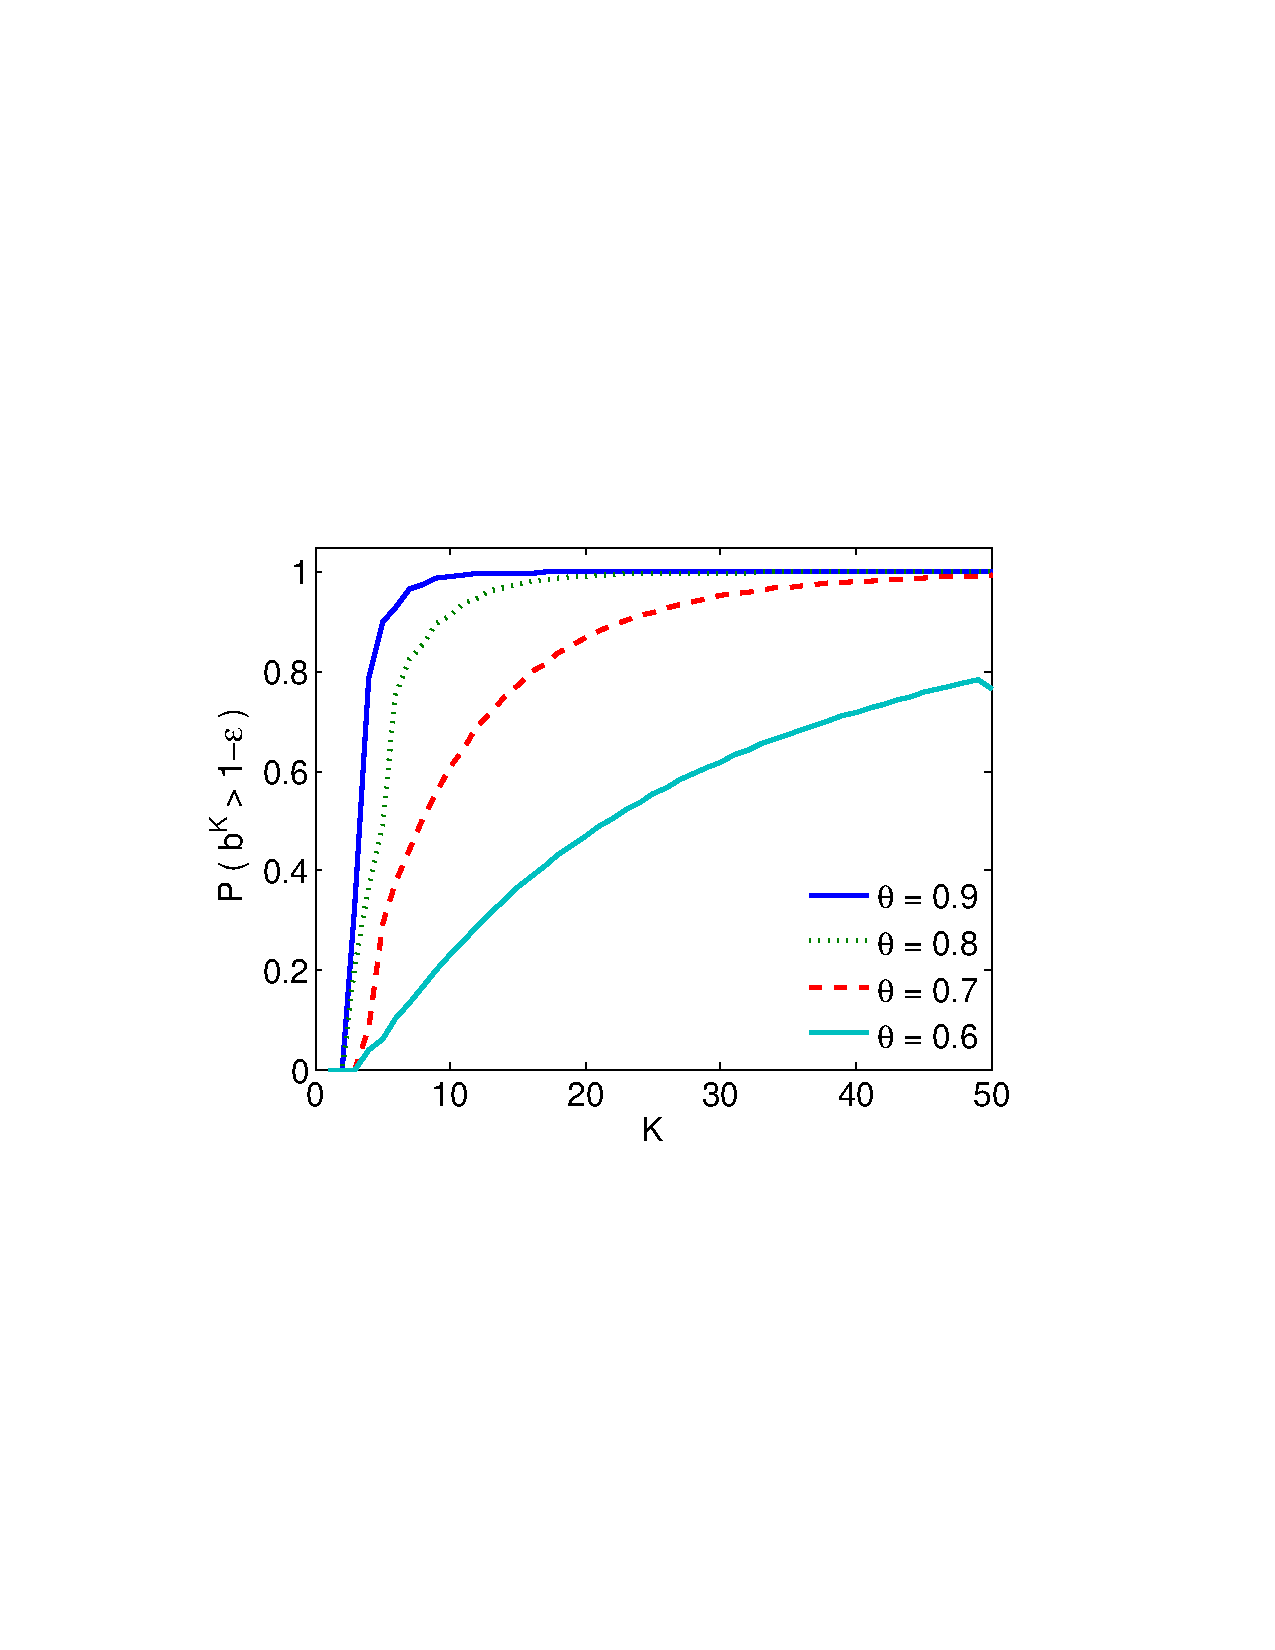
\includegraphics[width=.6\textwidth]{proba}
\end{center}
\caption[Probabilit� d'�tre dans un �tat de croyance d�terministe selon le nombre d'�tapes.]{\label{fig:probaLin}Probabilit� d'�tre dans un �tat de croyance d�terministe selon le nombre d'�tapes pour diff�rentes probabilit�s d'observation. $\nu = 100$ et $\varepsilon = 10^{-3}$.}
\end{figure}

\subsection{Et si les transitions sont stochastiques ?}\label{anx:it}

Si l'on regarde en particulier l'information contenue dans l'�tat de croyance en mesurant l'\emph{entropie} (c.f. sous-section suivante) de celui-ci, on peut voir qu'elle converge \emph{en moyenne} vers zero. N�anmoins, lorsque les transitions ne sont pas d�terministes, i.e. que de l'incertitude r�appara�t � chaque action effectu�e, une \emph{entropie r�siduelle moyenne} persiste comme d�montr� par les figures~\ref{fig:entropy:3} �~\ref{fig:entropy:97}. Plus pr�cis�ment, ces figures montrent l'�volution moyenne de l'entropie sur 10000 s�quences d'�tats de croyance lorsque les transitions sont � peine stochastiques et pour diff�rentes valeurs de la probabilit� minimale d'observation $\theta$.

\begin{figure}[!htb]
\begin{center}
\subfigure[\label{fig:entropy:3}]{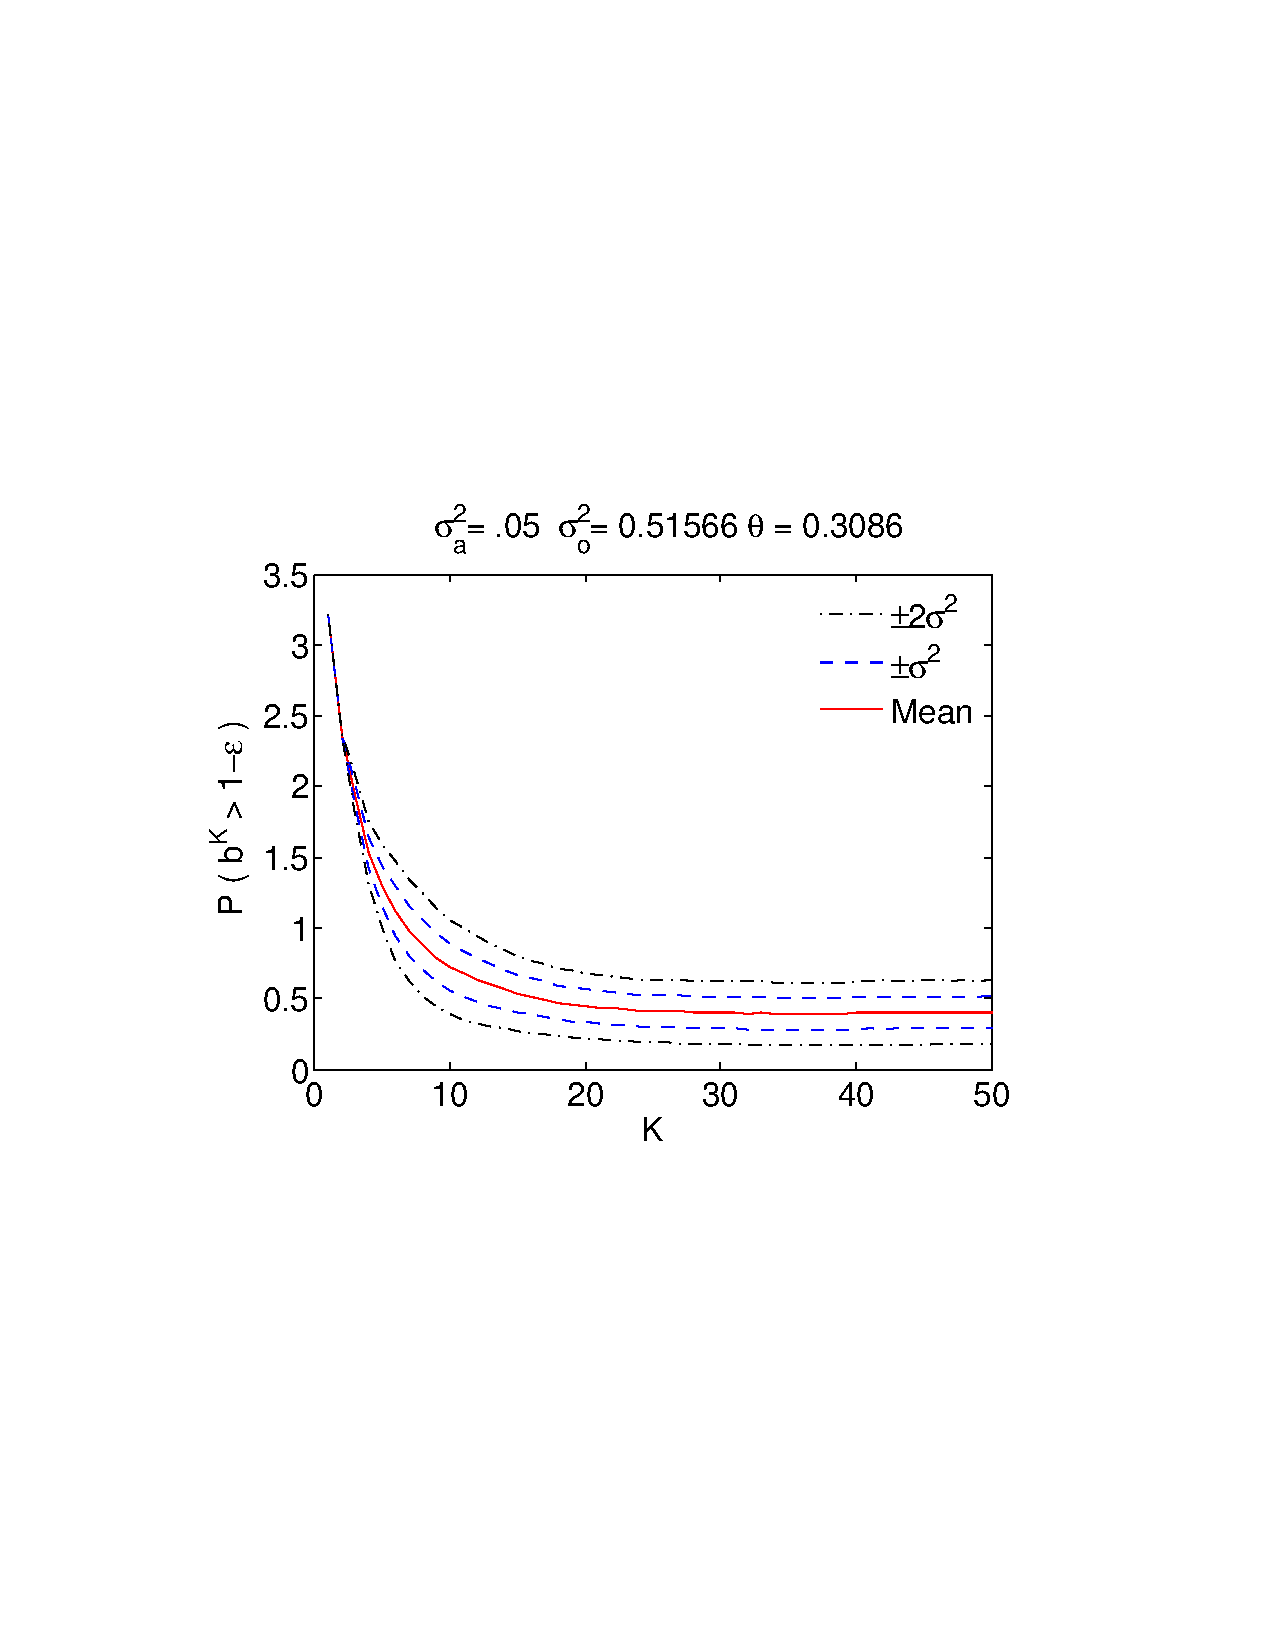
\includegraphics[width=.48\textwidth]{3}}~
\subfigure[\label{fig:entropy:5}]{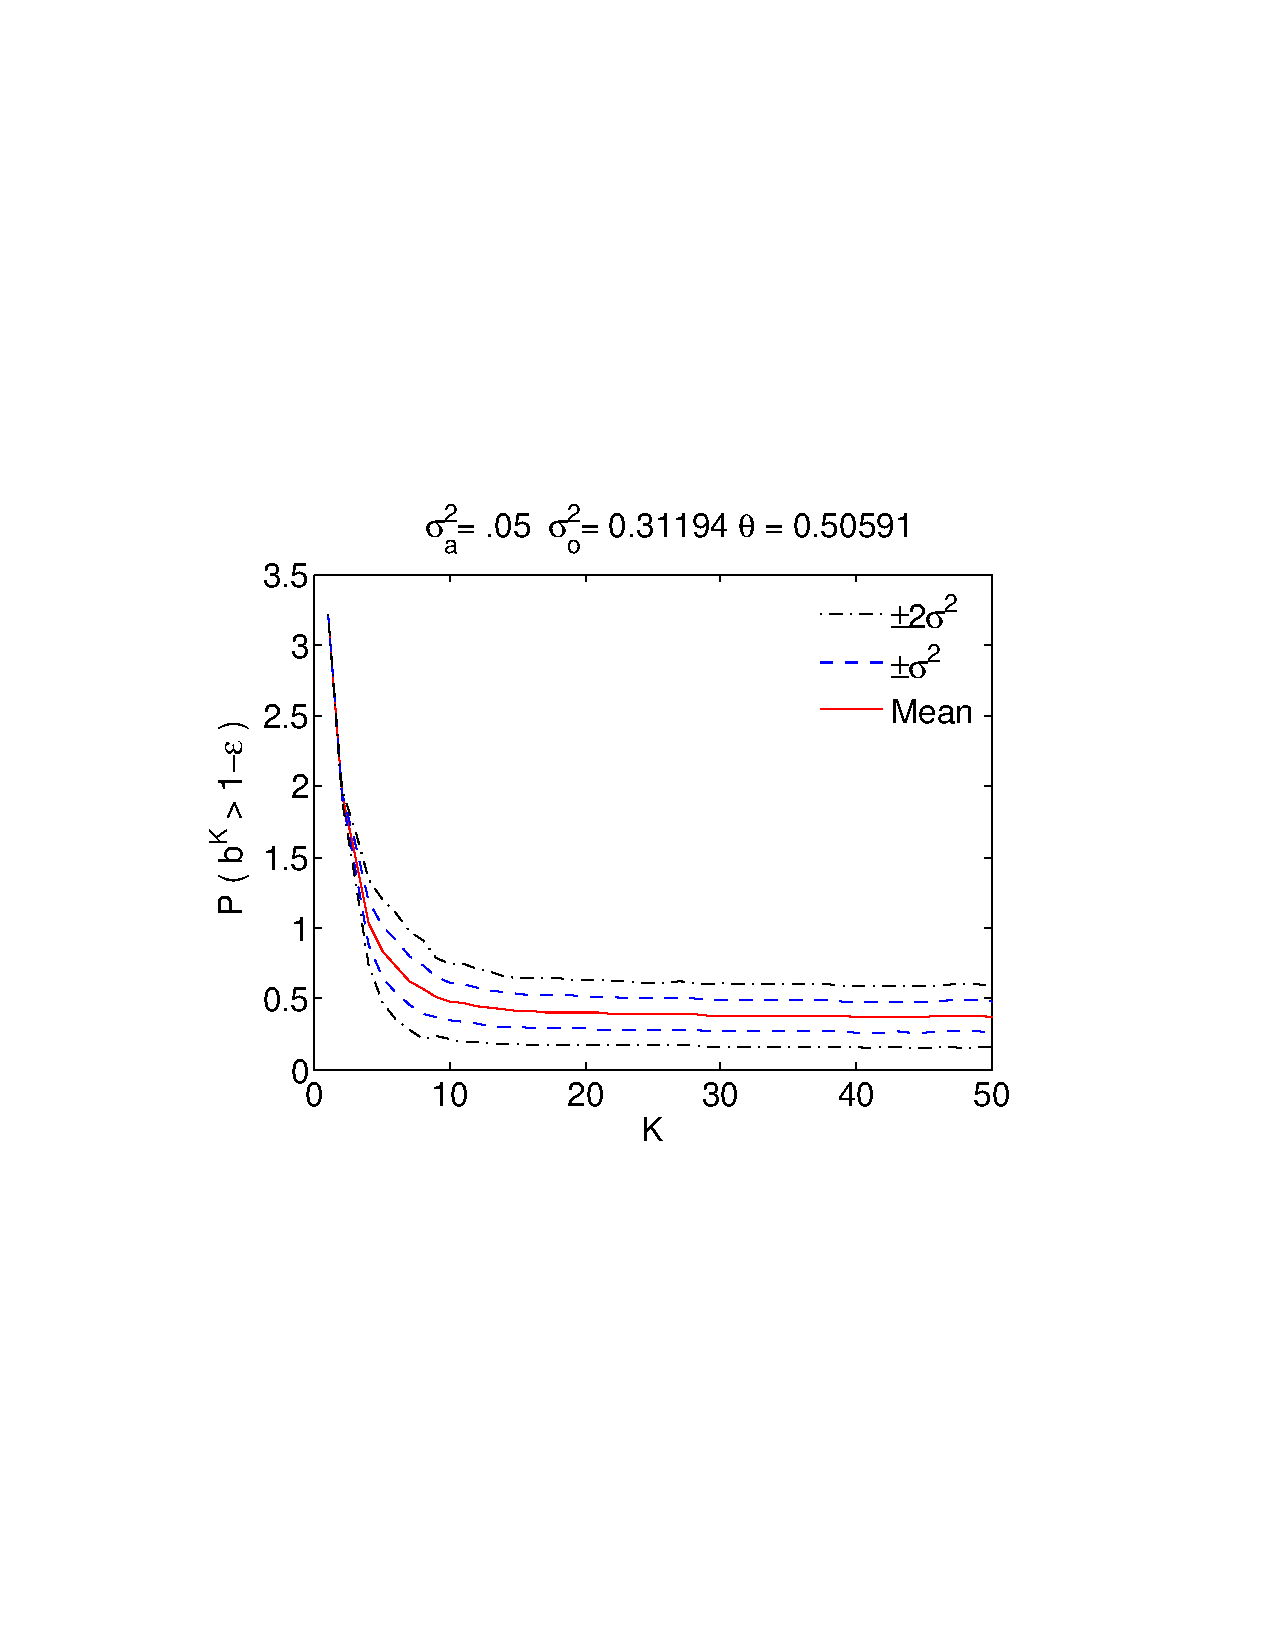
\includegraphics[width=.48\textwidth]{5}}\\
\subfigure[\label{fig:entropy:6}]{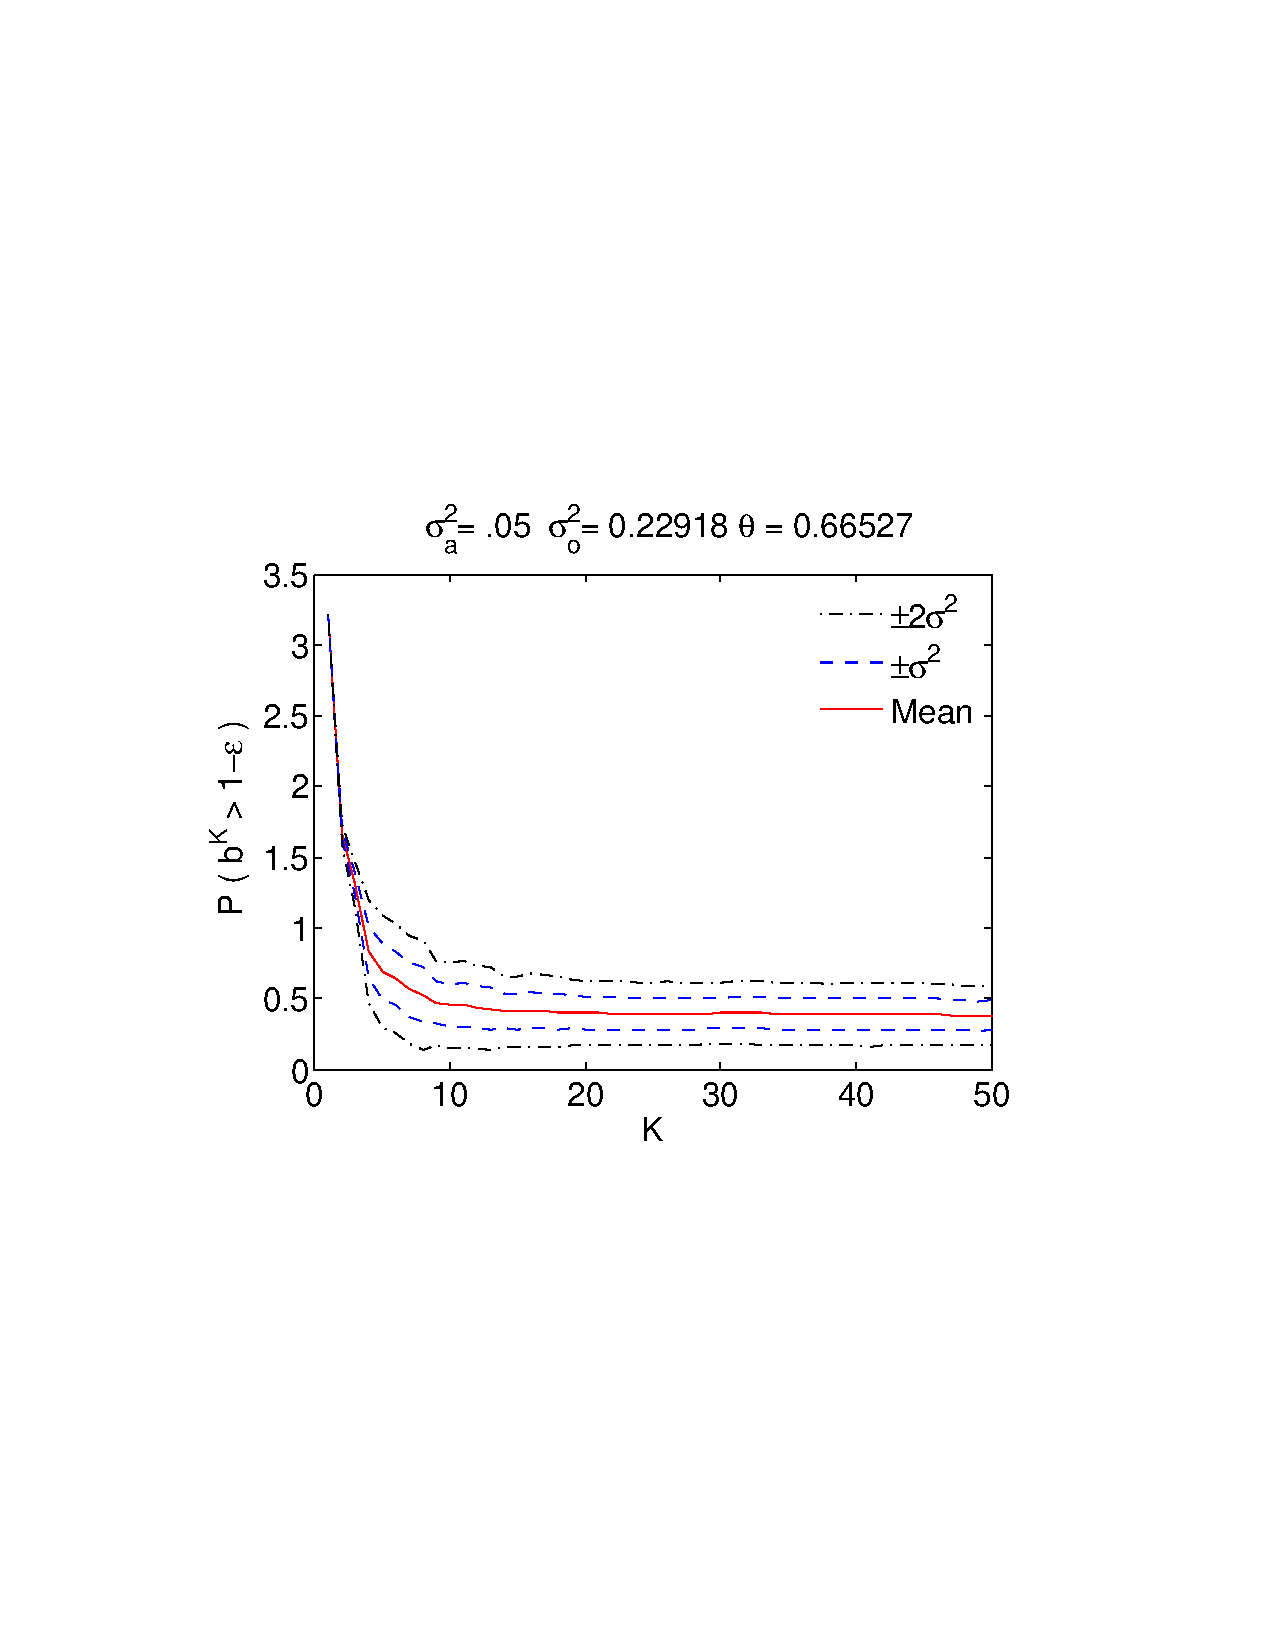
\includegraphics[width=.48\textwidth]{6}}~
\subfigure[\label{fig:entropy:7}]{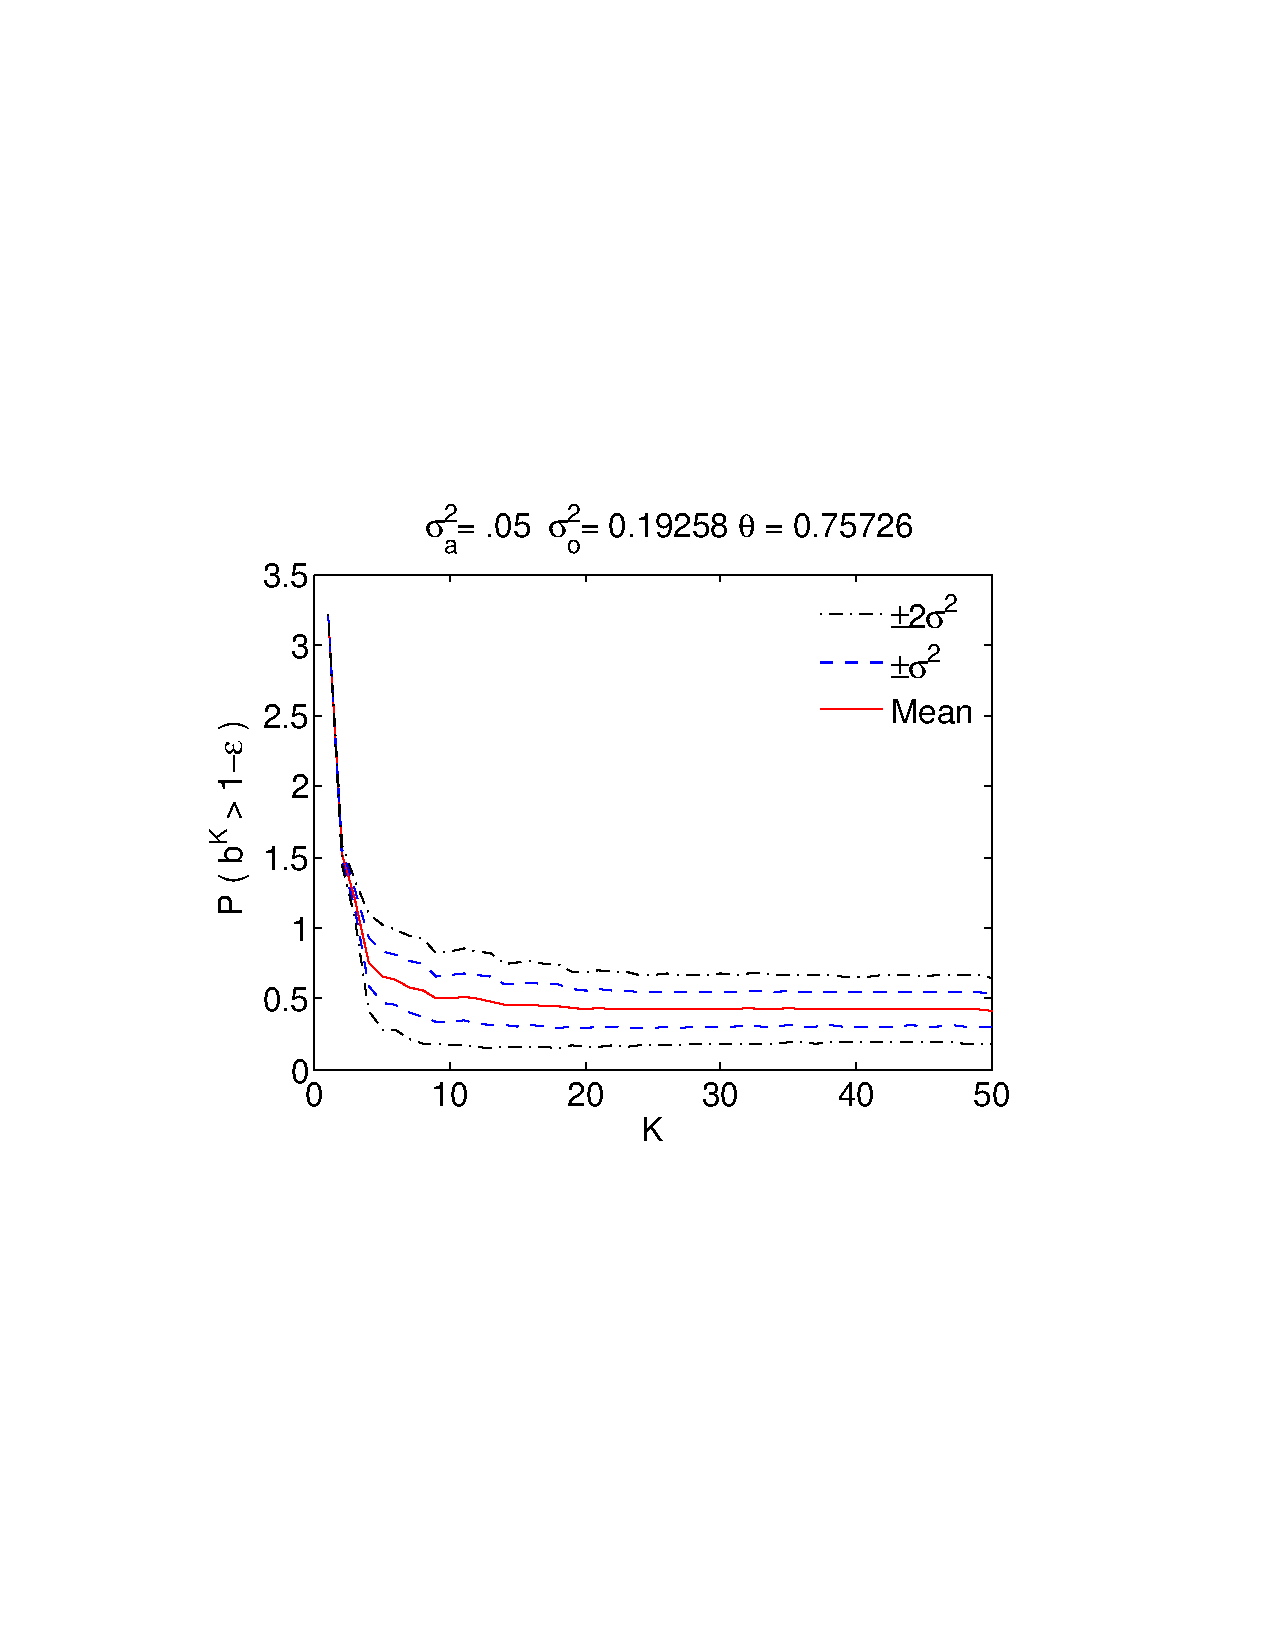
\includegraphics[width=.48\textwidth]{7}}\\
\subfigure[\label{fig:entropy:92}]{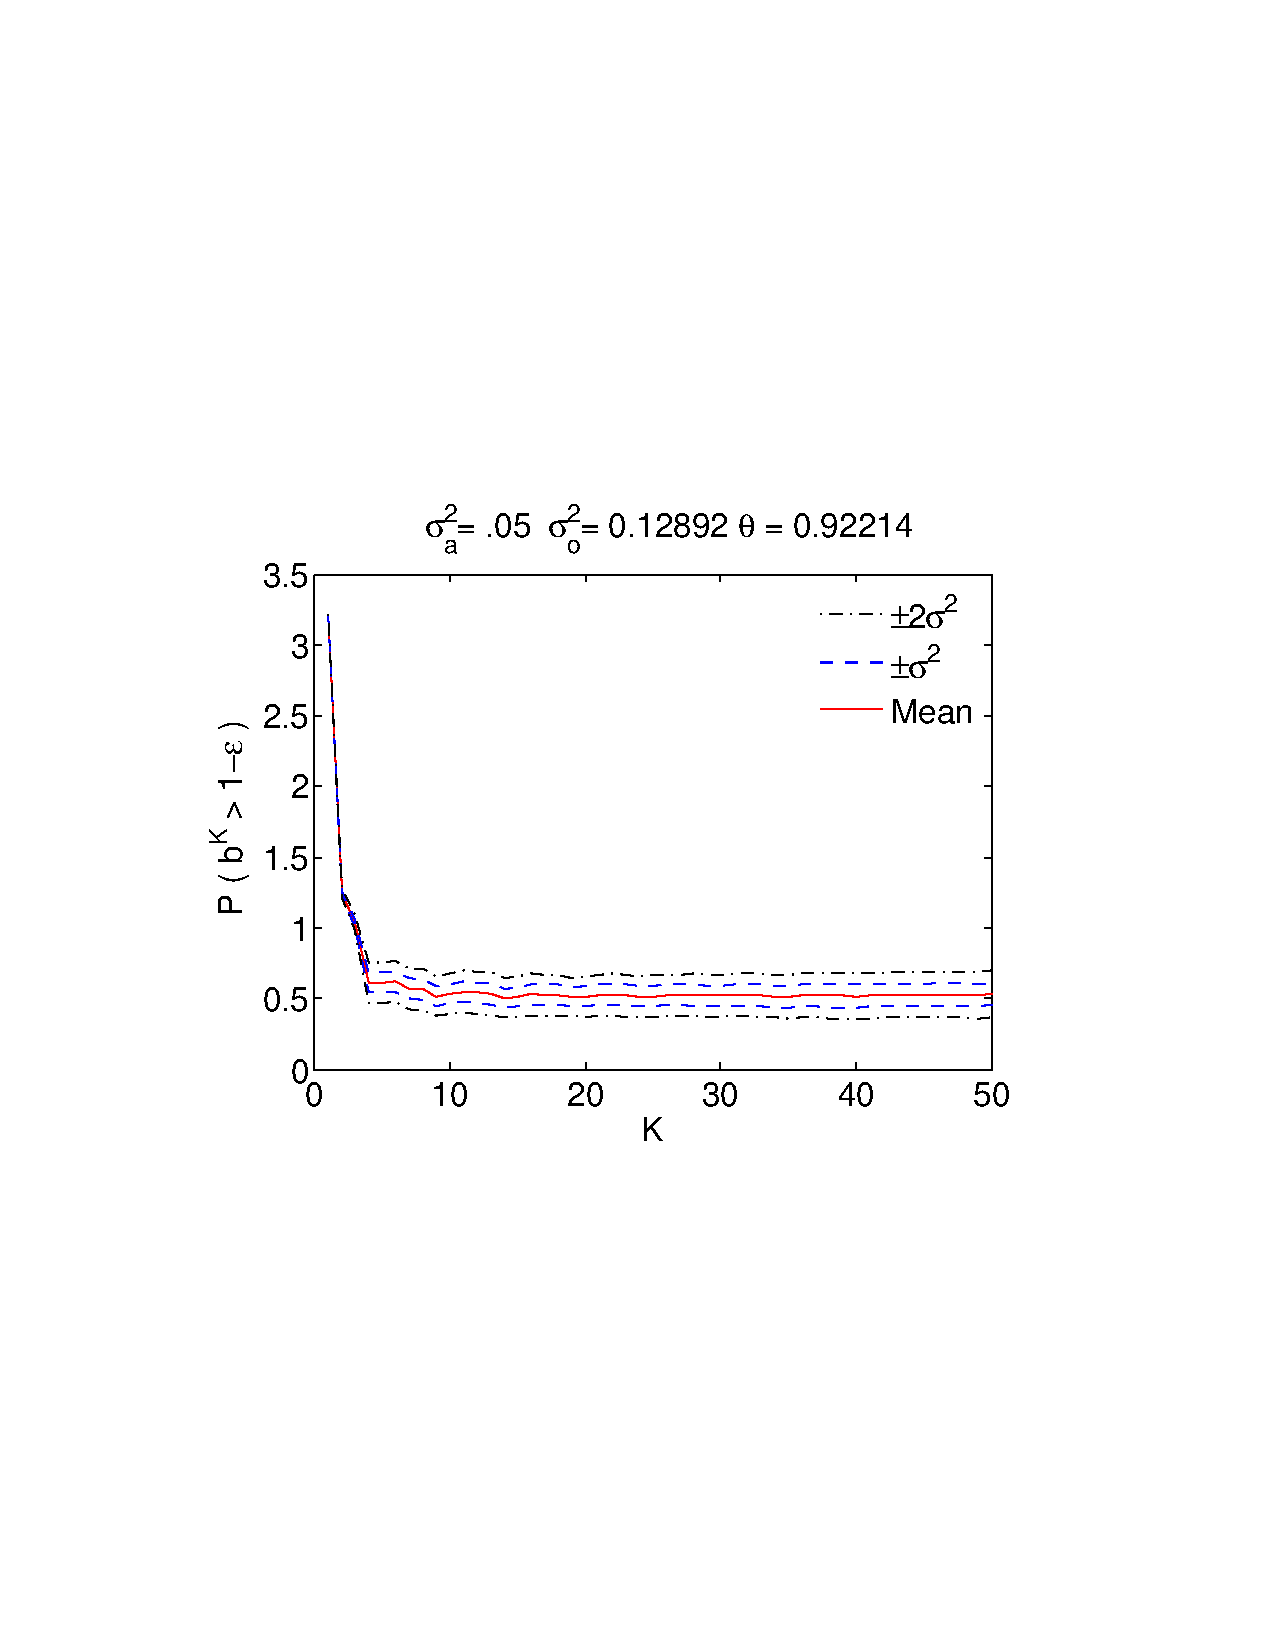
\includegraphics[width=.48\textwidth]{92}}~
\subfigure[\label{fig:entropy:97}]{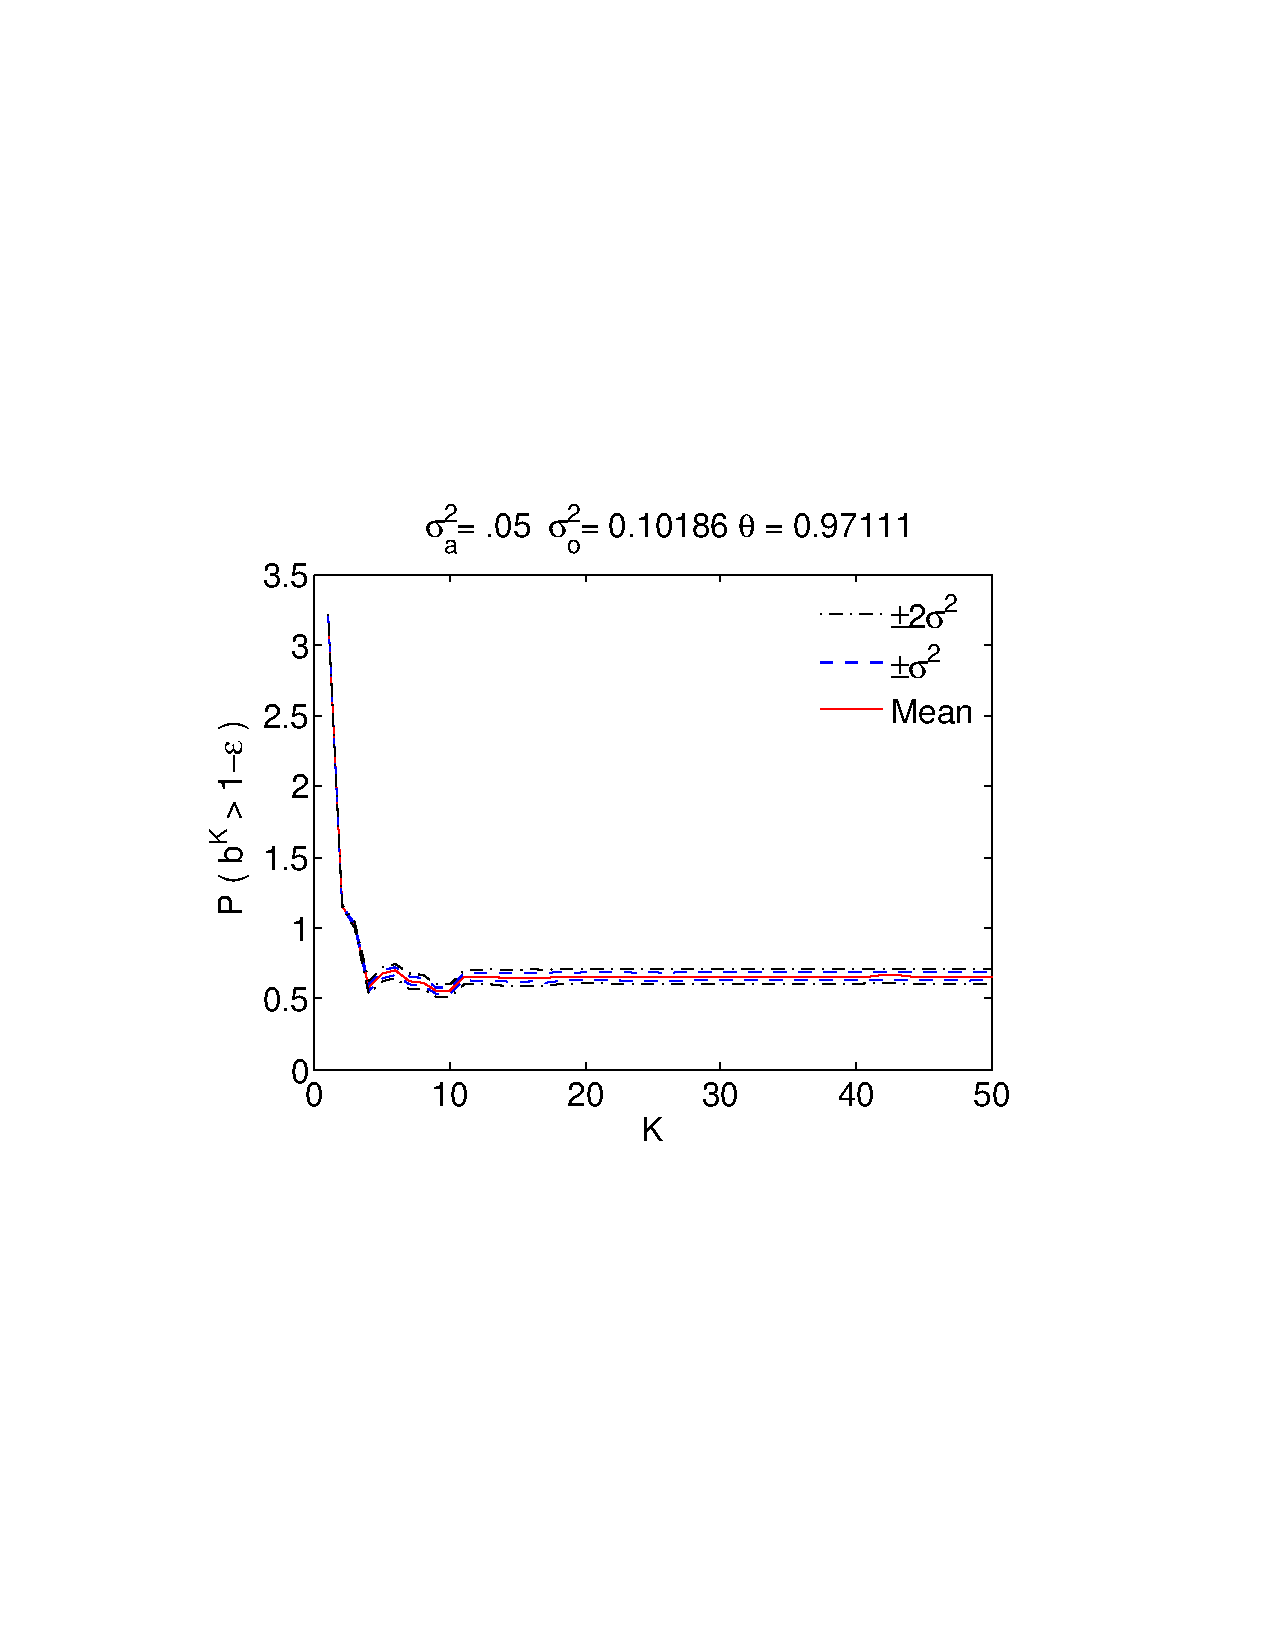
\includegraphics[width=.48\textwidth]{97}}
\end{center}
\caption[Entropie de l'�tat de croyance avec transitions stochastiques.]{\label{fig:entropy} �volution de l'entropie de l'�tat de croyance au cours du temps pour diff�rentes valeurs de $\theta$ et en presence d'incertitude sur les transitions.}
\end{figure}

\subsubsection{Entropie d'un �tat de croyance}

Une mesure couramment utilis�e en th�orie de l'information de la quantit� d'information et de la qualit� de l'information contenue dans un distribution de probabilit� telle que l'estimation d'un �tat de croyance~\citep{FBT.98} est l'entropie de~\cite{S.48}. L'entropie mesure la quantit� d'incertitude contenue dans une distribution de probabilit� discr�te ou continue. Dans le cas particulier d'un �tat de croyance sur un ensemble fini d'�tats, l'entropie $H$ est calcul�e en utilisant la formule suivante:
\begin{equation}\label{aeq:entropy}
    H(\bel^t) = -\sum_{s\in\Sta} \bel^t(s) \log \bel^t(s)
\end{equation}
L'entropie est maximale est �gale � $\log|\Sta|$ lorsque l'�tat de croyance est uniforme -- i.e il est possible d'�tre dans tous les �tats de mani�re �quiprobable -- et tend vers zero � mesure que l'�tat de croyance devient d�terministe\footnote{Par convention, $0\log 0\equiv 0$.}.

Dans la litt�rature de la th�orie de l'information, l'entropie associ�e � l'estimation de l'�tat courant a rarement �t� �tudi�e, except� par~\cite{R.06} qui a appel� cette quantit� \emph{entropie d'estimation}. En fait, cette entropie d'estimation, que nous noterons  $H(\bel^t)$, est �gale � l'entropie de la distribution sur les �tats �tant donn�e une s�quence d'observations re�ues. Elle se calcule donc de la mani�re suivante:
\begin{equation}\label{aeq:EstimationEntropy}
    H(\bel^t) = H(s^t|o^t,o^{t-1},\dots,o^1) = H(s^t|o^t,\bel^{t-1})
\end{equation}

Ainsi, en utilisant les r�gles connues de th�orie de l'information, il est possible d'�noncer la proposition suivante:
\begin{proposition}\label{ap:beliefEntropy} L'entropie $H(\bel^t)$ d'un �tat de croyance � l'�tape $t$ depuis un �tat de croyance $\bel^{t-1}$ �tant donn�e n'importe quelle politique est donn�e par l'�quation suivante:
\begin{equation}\label{aeq:beliefEntropyF}
H(\bel^t) = H(s^t) - I(s^t;\bel^{t-1}) - I(o^t;s^t|\bel^{t-1}) \qquad
\end{equation}
\end{proposition}
\begin{proof}\begin{eqnarray}
  H(\bel^t)  &=& H(o^t|s^t,\bel^{t-1}) - H(o^t|\bel^{t-1}) + H(s^t|\bel^{t-1})\notag\\
             &=& - I(o^t;s^t|\bel^{t-1}) + H(s^t|\bel^{t-1})\notag\\
   \mbox{since }I(X;Y)  &=& H(X) - H(X|Y)\notag%\\
\end{eqnarray}
O� $H(s^t)$ est le \emph{taux instantan� d'entropie}~\citep{CT.91} de la cha�ne de Markov sous-jacente � la politique qui se construit par la combinaison de la politique et de la fonction de transition. $I(s^t;\bel^{t-1})$ est l'\emph{information mutuelle} entre l'�tat $s^t$ et l'�tat de croyance � l'�tape $t-1$ et $I(o^t;s^t|\bel^{t-1})$ l'\emph{information mutuelle conditionnelle} entre l'�tat $s^t$ et l'observation $o^t$ �tant donn� l'�tat de croyance � l'�tape pr�c�dente.
\end{proof}

L'information mutuelle mesure l'ind�pendance mutuelle de deux variables al�atoires ou la quantit� d'information que deux variables al�atoires partagent. Elle est donn�e par:
\begin{eqnarray*}
I(X;Y) & = & \sum_{y \in Y} \sum_{x \in X} p(x,y) \log{ \left( \frac{p(x,y)}{p_1(x)\,p_2(y)} \right) }, \,\! \\
&  = & H(X) - H(X|Y) \\
&  = & H(Y) - H(Y|X) \\
&  = & H(X) + H(Y) - H(X,Y) \\
&  = & H(X,Y) - H(X|Y) - H(Y|X).
\end{eqnarray*}

L'information mutuelle conditionnelle mesure la m�me quantit� d'information, mais �tant donn�e une troisi�me variable al�atoire:
\[I(X;Y|Z) = \mathbb E_Z \big(I(X;Y)|Z\big)
    = \sum_{z\in Z} \sum_{y\in Y} \sum_{x\in X}
      p_Z(z) p_{X,Y|Z}(x,y|z) \log \frac{p_{X,Y|Z}(x,y|z)}{p_{X|Z}(x|z)p_{Y|Z}(y|z)},\]
Qui peut �tre simplifi�e en:
\[I(X;Y|Z) = \sum_{z\in Z} \sum_{y\in Y} \sum_{x\in X}
      p_{X,Y,Z}(x,y,z) \log \frac{p_Z(z)p_{X,Y,Z}(x,y,z)}{p_{X,Z}(x,z)p_{Y,Z}(y,z)}.\]

De fait, dans le contexte d'information bijective exprim� par la d�finition~\ref{def:enough-obs} o� les observations apportent la m�me quantit� d'information quelque soit l'action effectu�e, il serait possible de croire que l'�quation~\eqref{aeq:beliefEntropyF} correspond � l'entropie de l'�tat de croyance sachant que l'observation $o^t$ a �t� re�ue quelque soit l'action effectu�e. En r�alit�, cette action effectu�e a un impact sur la fonction de transition, et ainsi la politique influence fortement l'entropie de l'�tat de croyance. L'entropie $H(\bel^t)$ peut donc �tre interpr�t�e comme l'incertitude ajout�e par la fonction de transition � laquelle on retranche l'information apport�e par l'observation $(I(o^t;s^t|\bel^{t-1}))$ et l'information d�j� contenue dans l'�tat de croyance � l'�tape pr�c�dente $(I(s^t;\bel^{t-1}))$.

Si l'on tente de sommer cette entropie r�cursive sur $K$ �tapes, on obtient:
\begin{corollary}\label{ac:beliefEntropy} L'entropie $H(\bel^K)$ d'un �tat de croyance apr�s $K$ �tapes depuis un �tat de croyance $\bel^0$ et �tant donn�e n'importe quelle politique est donn�e par:
\begin{equation}\label{aeq:beliefEntropyK}
H(\bel^K) = H(s^K) - \sum_{i=1}^K \left(I(s^i;\bel^{i-1}) + I(o^i;s^i|\bel^{i-1})\right)
\end{equation}
Sous la condition que $H(\bel^0) = H(s^0)$.
\end{corollary}
\begin{proof}Ce corollaire d�coule directement de la proposition~\ref{ap:beliefEntropy}.
\end{proof}

Dans cette formulation, $H(s^t)$ est toujours le taux d'entropie~\citep{CT.91} de la cha�ne de Markov sous-jacente. Ce taux d'entropie converge exponentiellement rapidement sous de petites hypoth�ses~\citep{HJ.99} vers
\begin{equation}\label{aeq:entropyRate}
H(s) = \sum_{s\in\Sta} \sum_{s'\in\Sta} \mu_{s} \Tra(s,\pi(s),s') \log \left[\Tra(s,\pi(s),s')\right]
\end{equation}
O� $\mu_s$ est la distribution stationnaire de la cha�ne de Markov construite par la combinaison de la politique et de la fonction de transition.

Toutefois, aucune recherche � notre connaissance ne fait �tat de l'�volution de ce terme au cours du temps. La majorit� des recherches � ce sujet portent essentiellement sur l'�tude en \emph{r�gime d'�quilibre}, i.e. lorsque la cha�ne de Markov est cens�e avoir d�j� converg� vers sa distribution stationnaire et ne d�pend alors plus de la distribution initiale $\bel^0$. Certains travaux~\citep{Su.76,L.81,BG.78} expliquent qu'il existe des conditions sur la cha�ne permettant la convergence vers la distribution stationnaire en un nombre d'�tapes born�es, mais une adaptation reste � faire quant aux processus d�cisionnels puisque ces travaux restent sur les versions sans contr�le des cha�nes de Markov. Tr�s r�cemment des travaux de physique quantique semblent �galement faire �tat de r�sultats en r�gime non stationnaire du taux d'entropie, mais sont rest�s herm�tiques � notre compr�hension.

Voyons plut�t exp�rimentalement quelles sont les conditions sur la qualit� des transitions et des observations telles que l'agent soit capable d'extraire l'information exacte � propos de l'�tat sous-jacent de l'environnement.

\subsubsection{Exp�rimentations}

Pour tester ces valeurs de convergence de l'entropie, nous avons pris un probl�me simple de d�placement d'un robot sur une grille torique (une grille o� les cellules sur les bords sont adjointes au cellules du bord oppos�). Ce robot peut choisir de se d�placer dans les quatre directions cardinales ou de ne pas se d�placer, mais re�oit quand m�me � chaque �tape une observation. Cet agent conna�t �videmment les r�sultats esp�r�s de chacune de ses actions. Il sait �galement que, d� � certaines conditions environnementales, il peut glisser lors d'un de ses d�placements et se rendre dans une case adjacente � celle souhait�e initialement avec une certaine probabilit�. Nous supposons ici que l'action de ne pas se d�placer entra�ne �galement un glissement probable pour des raisons d'uniformit� dans la g�n�ration de l'entropie au cours du temps.

Nous avons choisi de repr�senter ces glissements par des distributions gaussiennes discr�tis�es puisque c'est souvent ainsi que les bruits sont repr�sent�s dans la litt�rature robotique. Ces glissements surgissent donc selon une distribution de probabilit� conjointe d�finie par une gaussienne discr�tis�e isotropique � deux dimensions param�tr�e par une variance $\sigma_\tau^2$. La figure~\ref{afig:tra} illustre donc la fonction de transition pour passer de l'�tat du centre de la grille � l'�tat en dessous par une distribution de probabilit� repr�sentant les chances de se retrouver dans les cases adjacentes.

\begin{figure}[t]
  \centering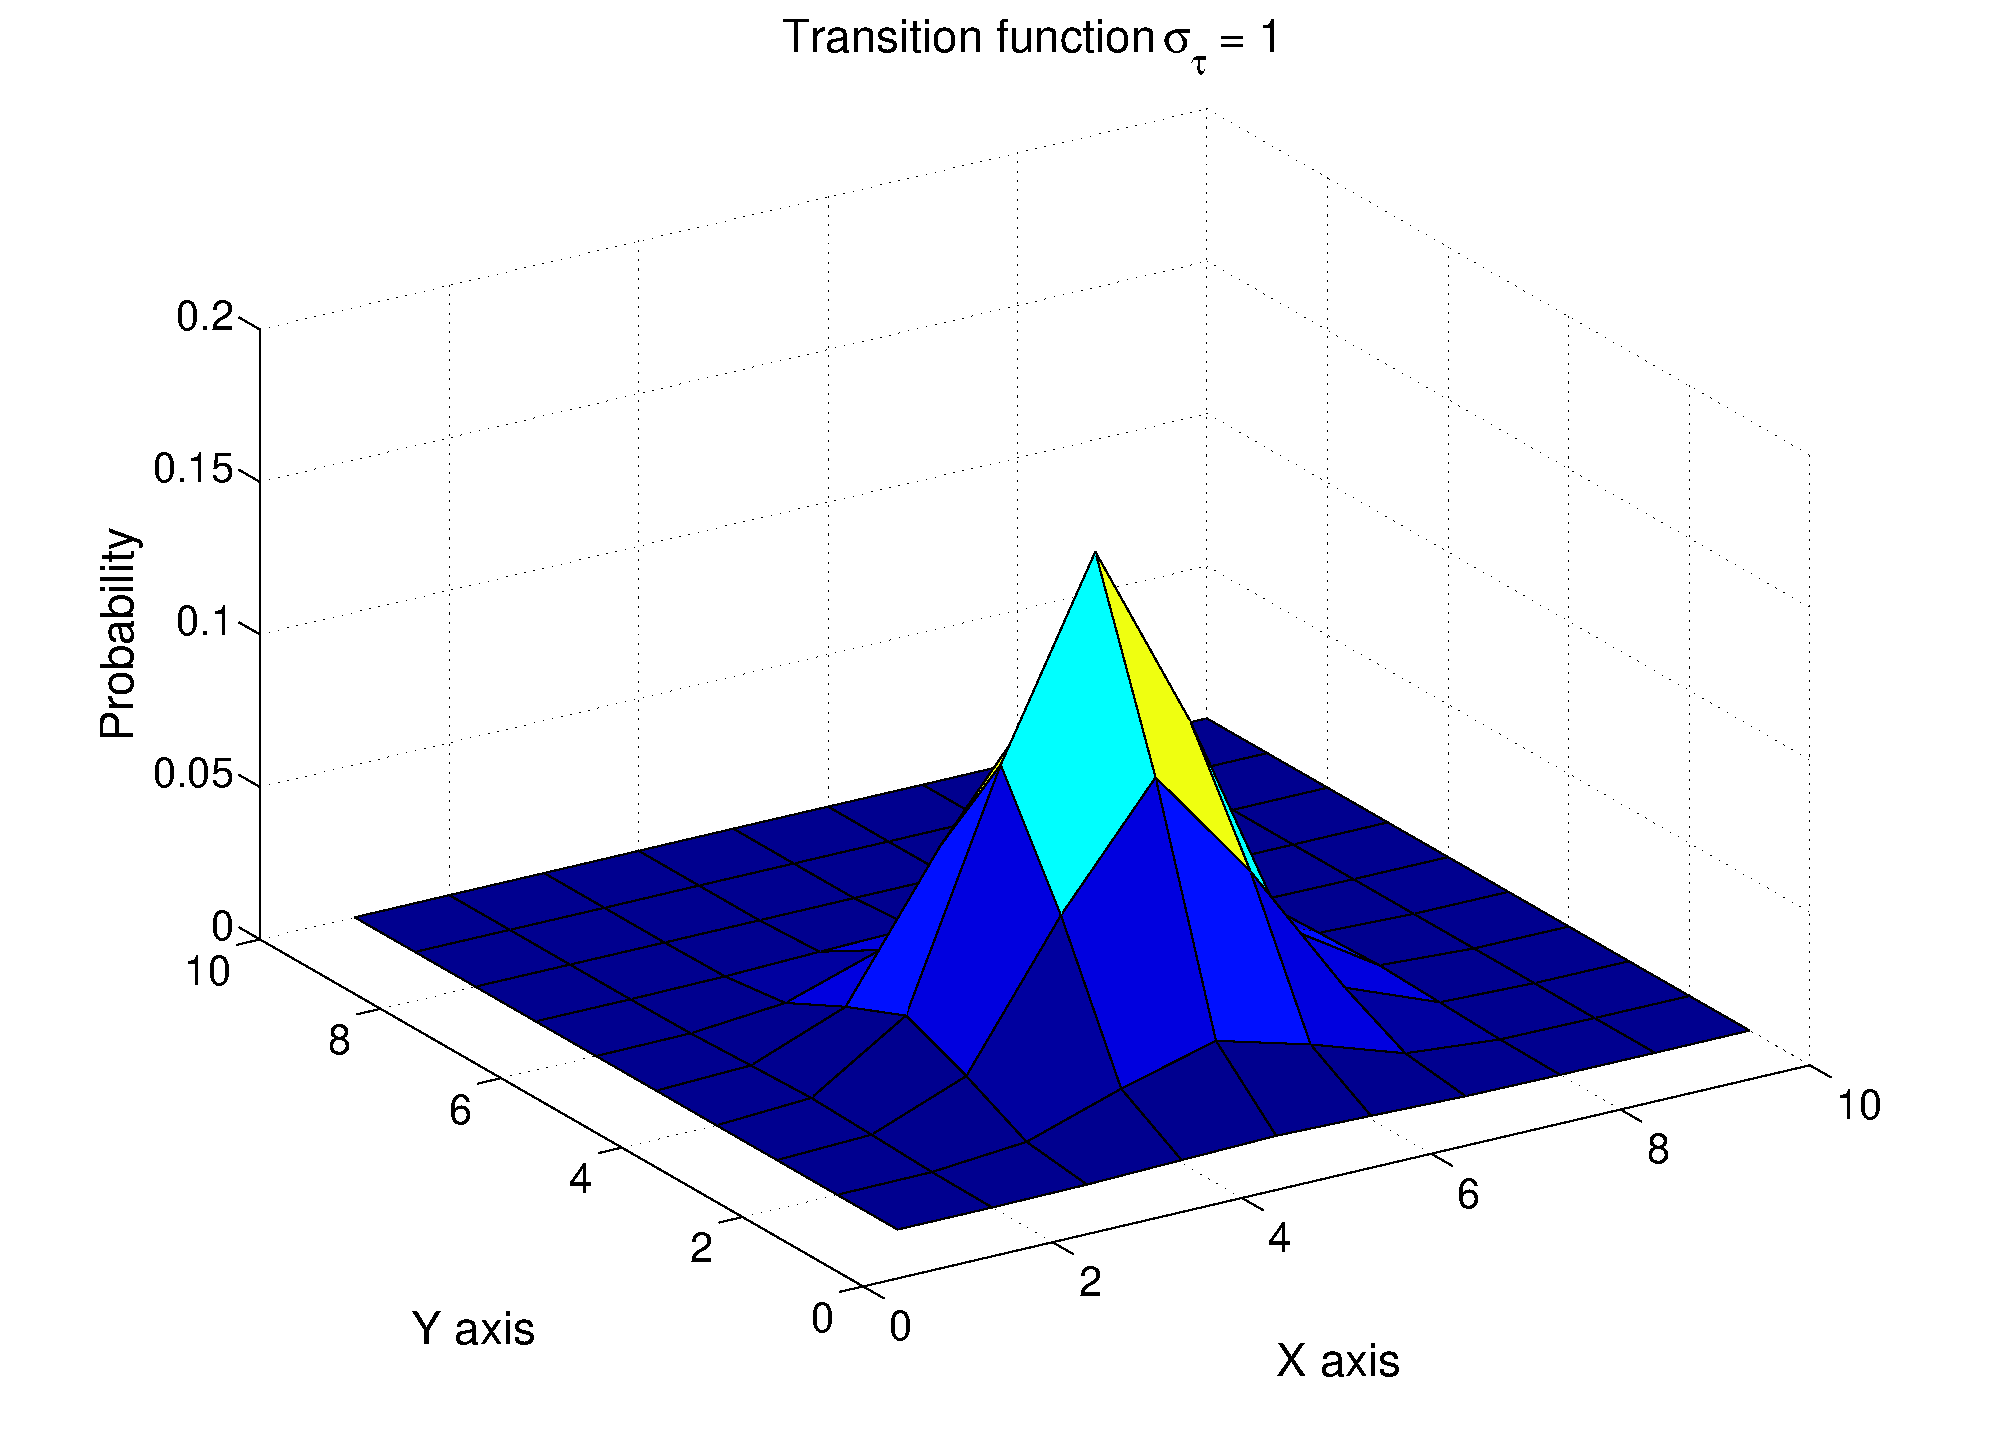
\includegraphics[width=.8\textwidth]{transitionPDF}
  \caption{Densit� de probabilit� de la fonction de transition depuis l'�tat $(5,5)$ au travers de l'action \textsc{down}. $\sigma_\tau = 1$.}\label{afig:tra}
\end{figure}

Comme nous l'avons dit ci-dessus, d�s que l'agent effectue une action, celui per�oit alors imm�diatement une observation de l'environnement (de son syst�me de positionnement global -- \textsc{gps} -- par exemple). Cette observation est aussi caract�ris�e par une distribution de probabilit� gaussienne discr�tis�e o� la moyenne est exactement l'�tat dans lequel est arriv� l'agent suite � son action et o� la variance est de $\sigma_o^2$. Cette distribution de probabilit� est donc similaire � celle de la fonction de transition et plus particuli�rement lorsque les variances sont �gales.

Puisque nous utilisons des distributions gaussiennes discr�tis�es sur une grille torique dans nos exp�rimentations, les r�sultats seront pr�sent�s par rapport � la variance des ces distributions. L'erreur relative de l'observation �tant donn�e la variance de la gaussienne est pr�sent�e dans la figure~\ref{afig:err}. Il convient de remarquer que cette erreur devient inf�rieure au milli�me lorsque la variance tombe en dessous de $0.3$. L'erreur sur les transitions �voluant de mani�re identique, nous ne la pr�sentons pas ici.

\begin{figure}[h!t]
  \centering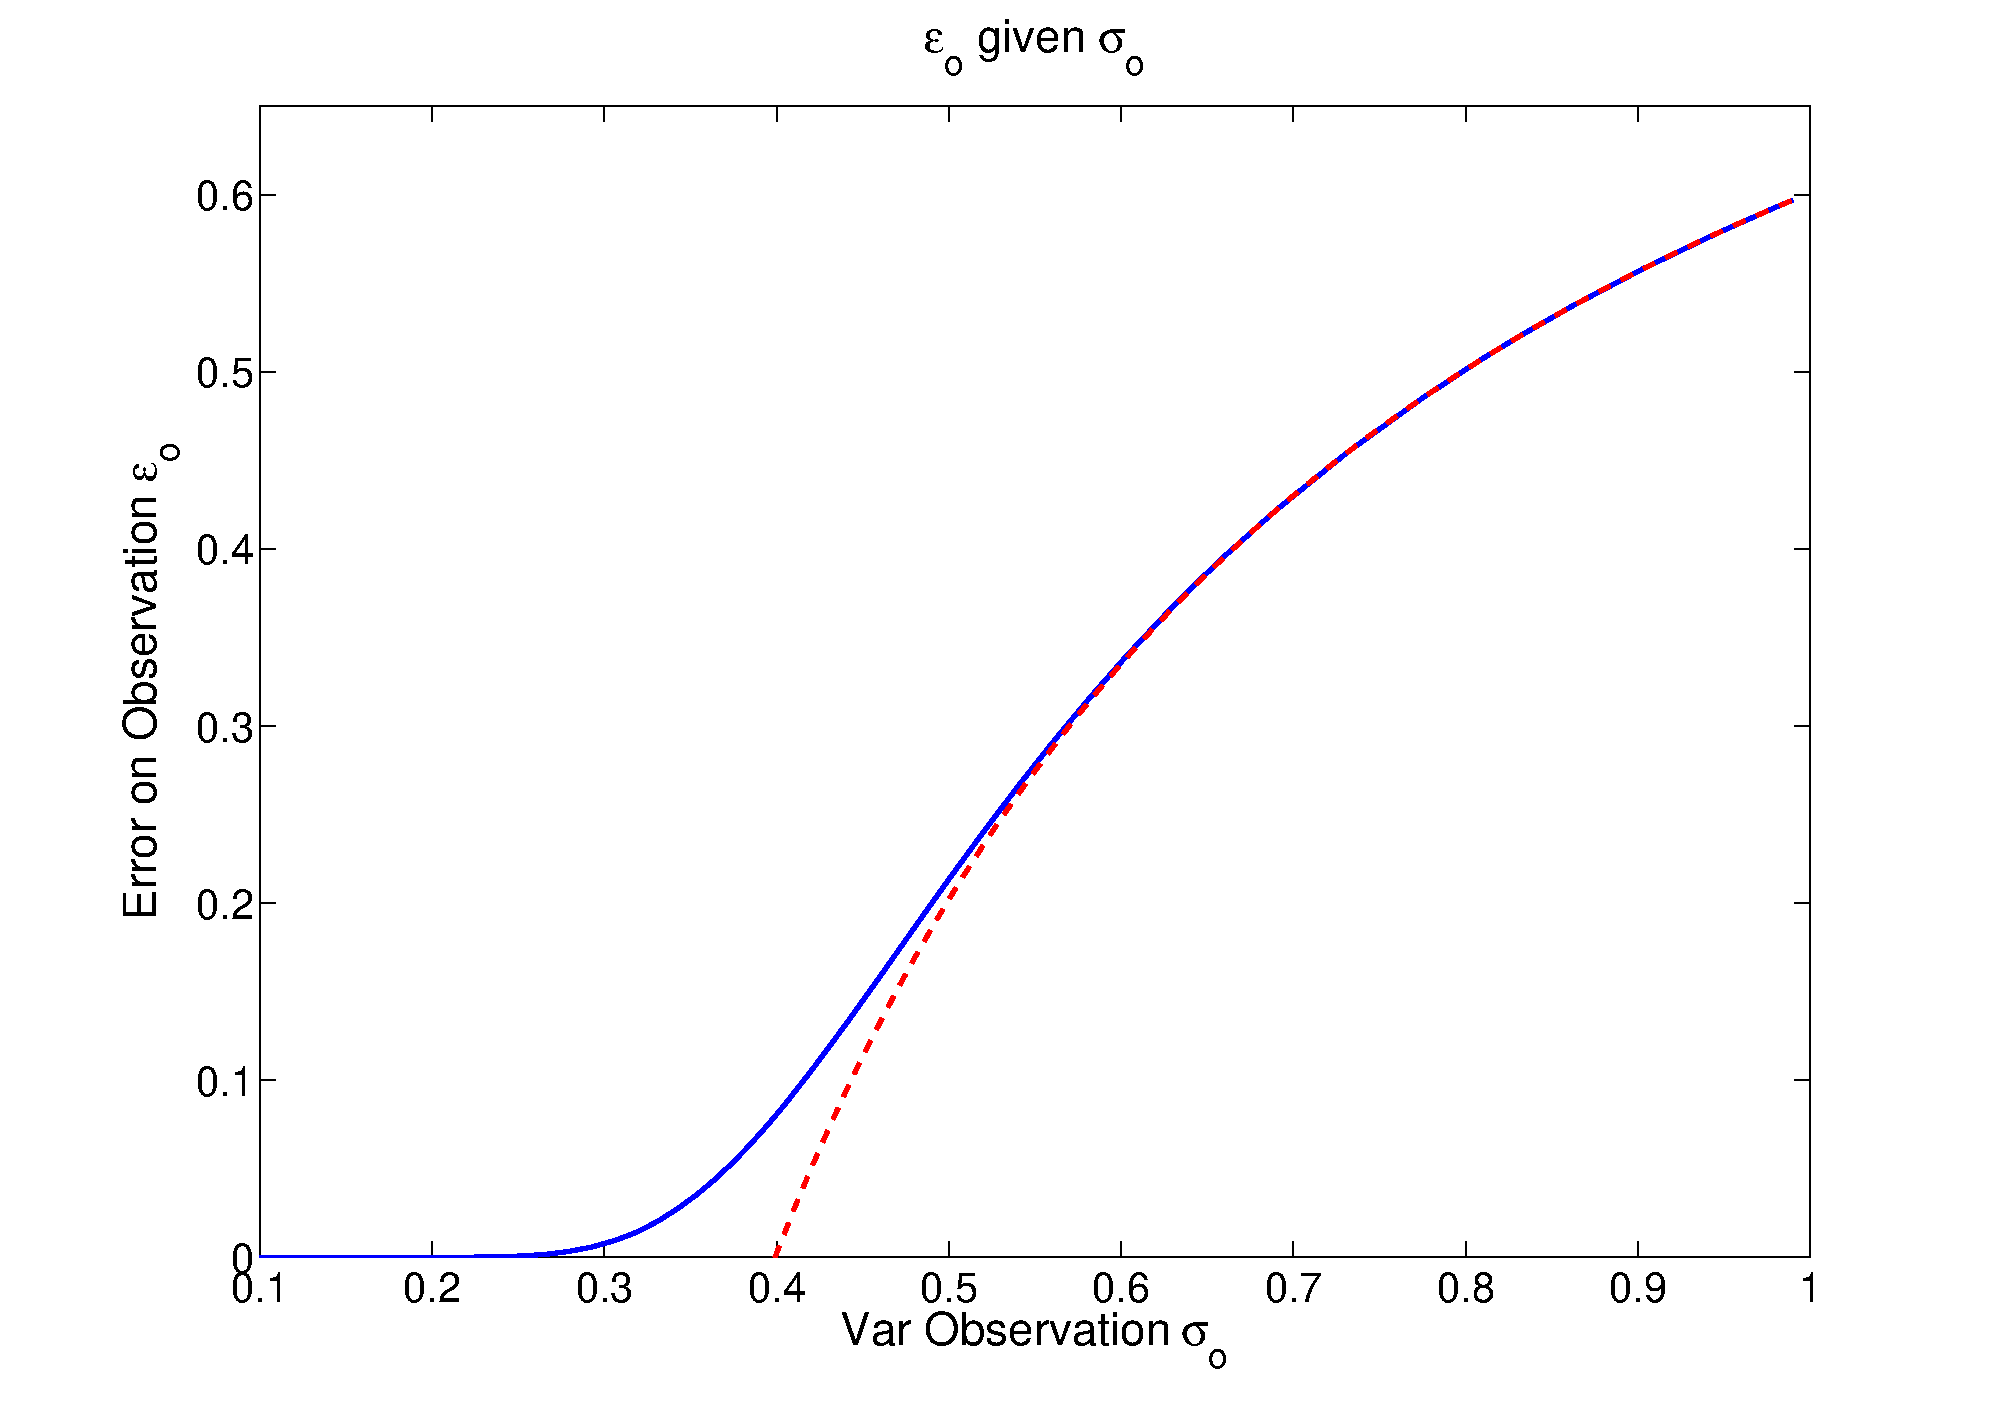
\includegraphics[width=.8\textwidth]{error}
  \caption[Erreur $\varepsilon_o$ sur l'observation.]{Erreur $\varepsilon_o$ sur l'observation �tant donn�e la variance de la gaussienne utilis�e pour repr�senter le bruit. L'erreur est repr�sent�e par la ligne pleine alors que la ligne hach�e repr�sente $1-\frac{1}{\sigma_o\sqrt{2\pi}}$.}\label{afig:err}
\end{figure}

La premi�re exp�rimentation que nous avons r�alis�e porte sur une politique al�atoire et nous calculons l'entropie d'estimation apr�s 3000 �tapes pour diff�rentes variances allant de 0 � 3. Nous ne pr�sentons toutefois que les r�sultats variant de 0.1 � 1, puisqu'en dessous de 0.1, la fonction \texttt{normpdf} de Matlab$^\circledR$ souffre de probl�mes de pr�cision, et au-del� de 0.8, le mode de la distribution devient plus petit que $1\slash 2$ et les r�sultats sont tr�s similaires � ceux pour des variances comprises entre 0.8 et 1.

\begin{figure}[h!t]
  \centering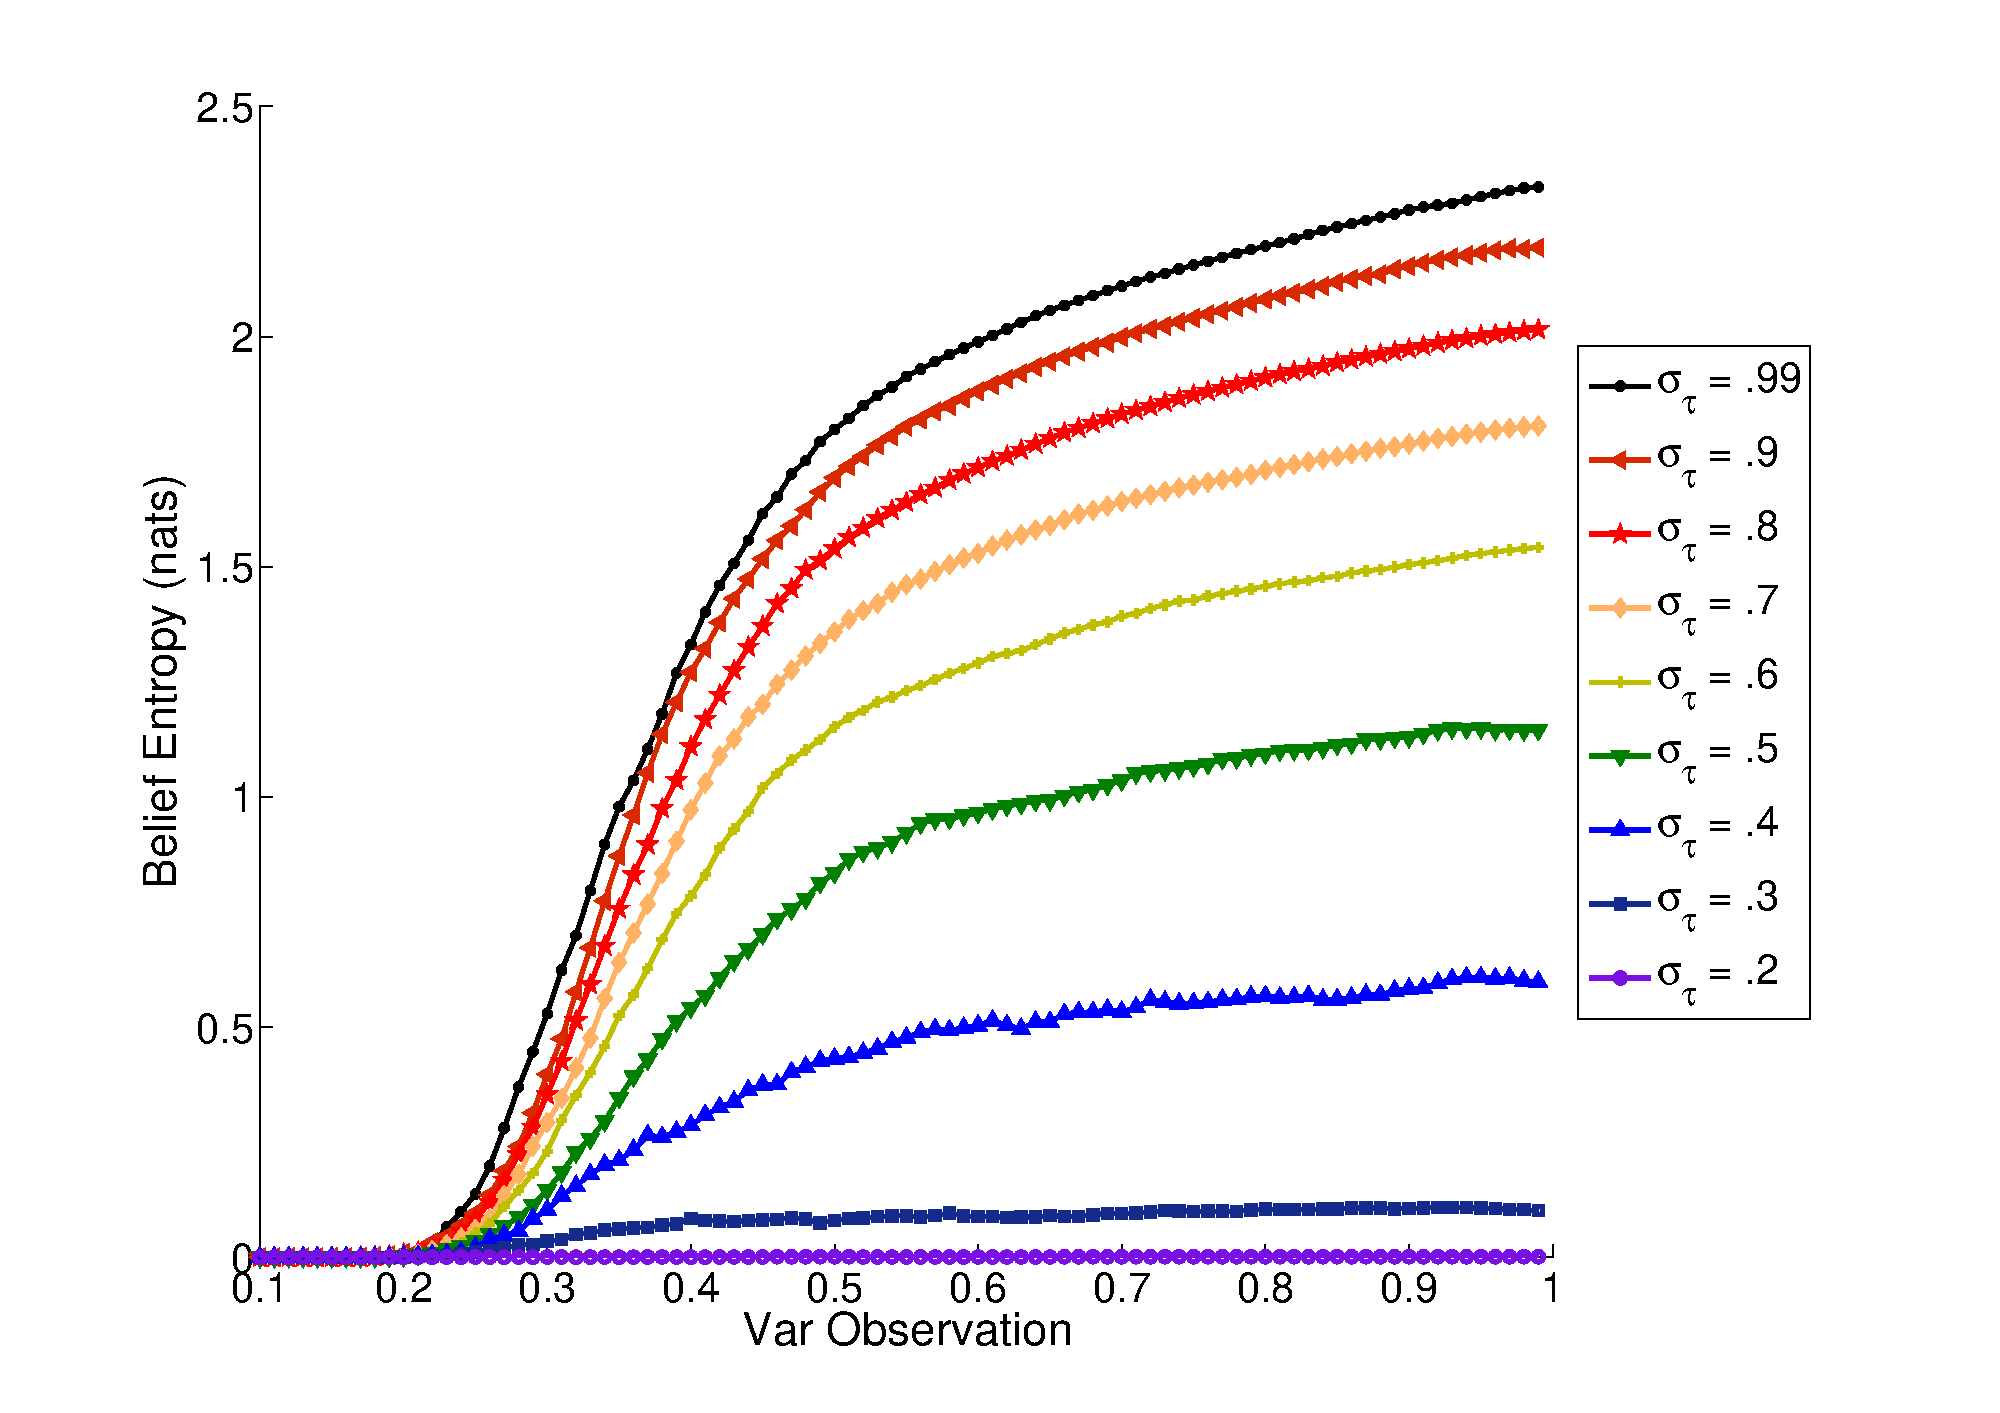
\includegraphics[width=.8\textwidth]{ent3000}
  \caption{Entropie de l'�tat de croyance $\bel^{3000}$ par rapport � diff�rentes valeurs de $\sigma_\tau$ et $\sigma_o$.}\label{afig:ent3000}
  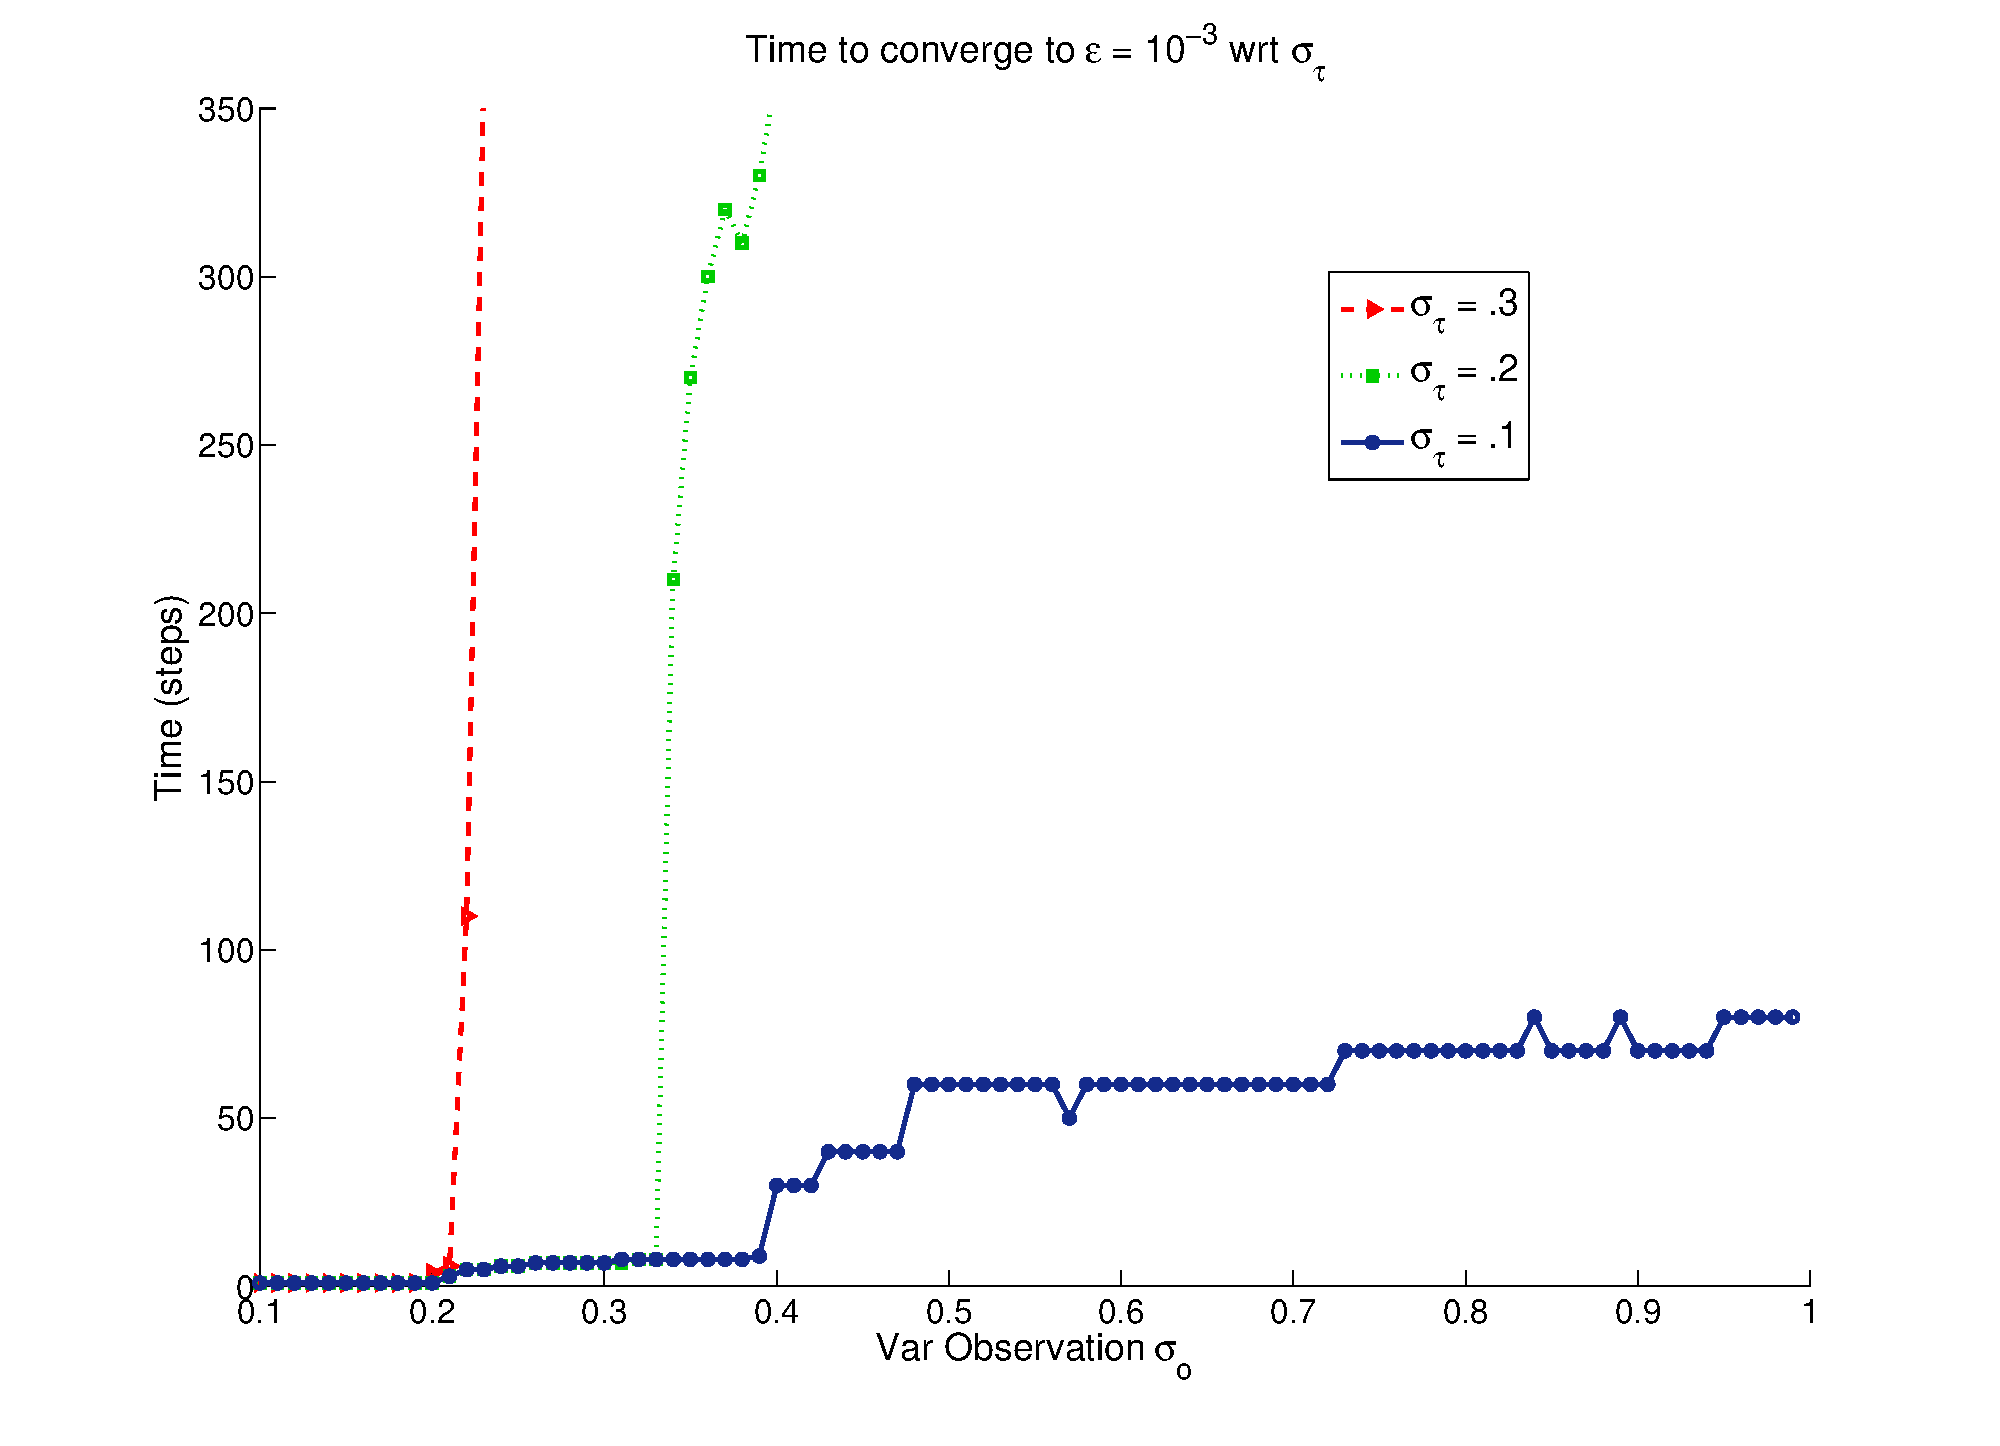
\includegraphics[width=.8\textwidth]{timeToConvZeroVarOnTra3}
  \caption[Temps minimal de convergence de l'entropie d'estimation avec politique al�atoire.]{Temps minimal de convergence de l'entropie d'estimation avec politique al�atoire pour diff�rentes variances sur la transition $\sigma_\tau$ et diff�rentes variances sur l'observation $\sigma_o$.}\label{afig:ConvTime}
\end{figure}

La figure~\ref{afig:ConvTime} montre le temps minimal de convergence sur 100 trajectoires pour que l'entropie de l'�tat de croyance converge vers $\varepsilon = 10^{-3}$ sous l'influence d'une politique al�atoire. Cette courbe mets en valeur la fait que, d�s que la politique fait en sorte que la cha�ne de Markov sous-jacente est ergodique, l'entropie peut prendre un temps exponentiel avant de converge vers $\varepsilon$, si seulement elle converge. En fait, les figures \ref{afig:belEnt1} � \ref{afig:belEnt50} montrent l'entropie � diff�rentes �tapes par rapport � la variance sur la transition et sur l'observation. Malheureusement, ces figures montrent �galement qu'il existe des valeurs de variance sur la transition qui induisent des valeurs de convergence de l'entropie largement sup�rieures � $\varepsilon$, comme il �tait possible de s'y attendre.

%\begin{figure}[t]
%  \centering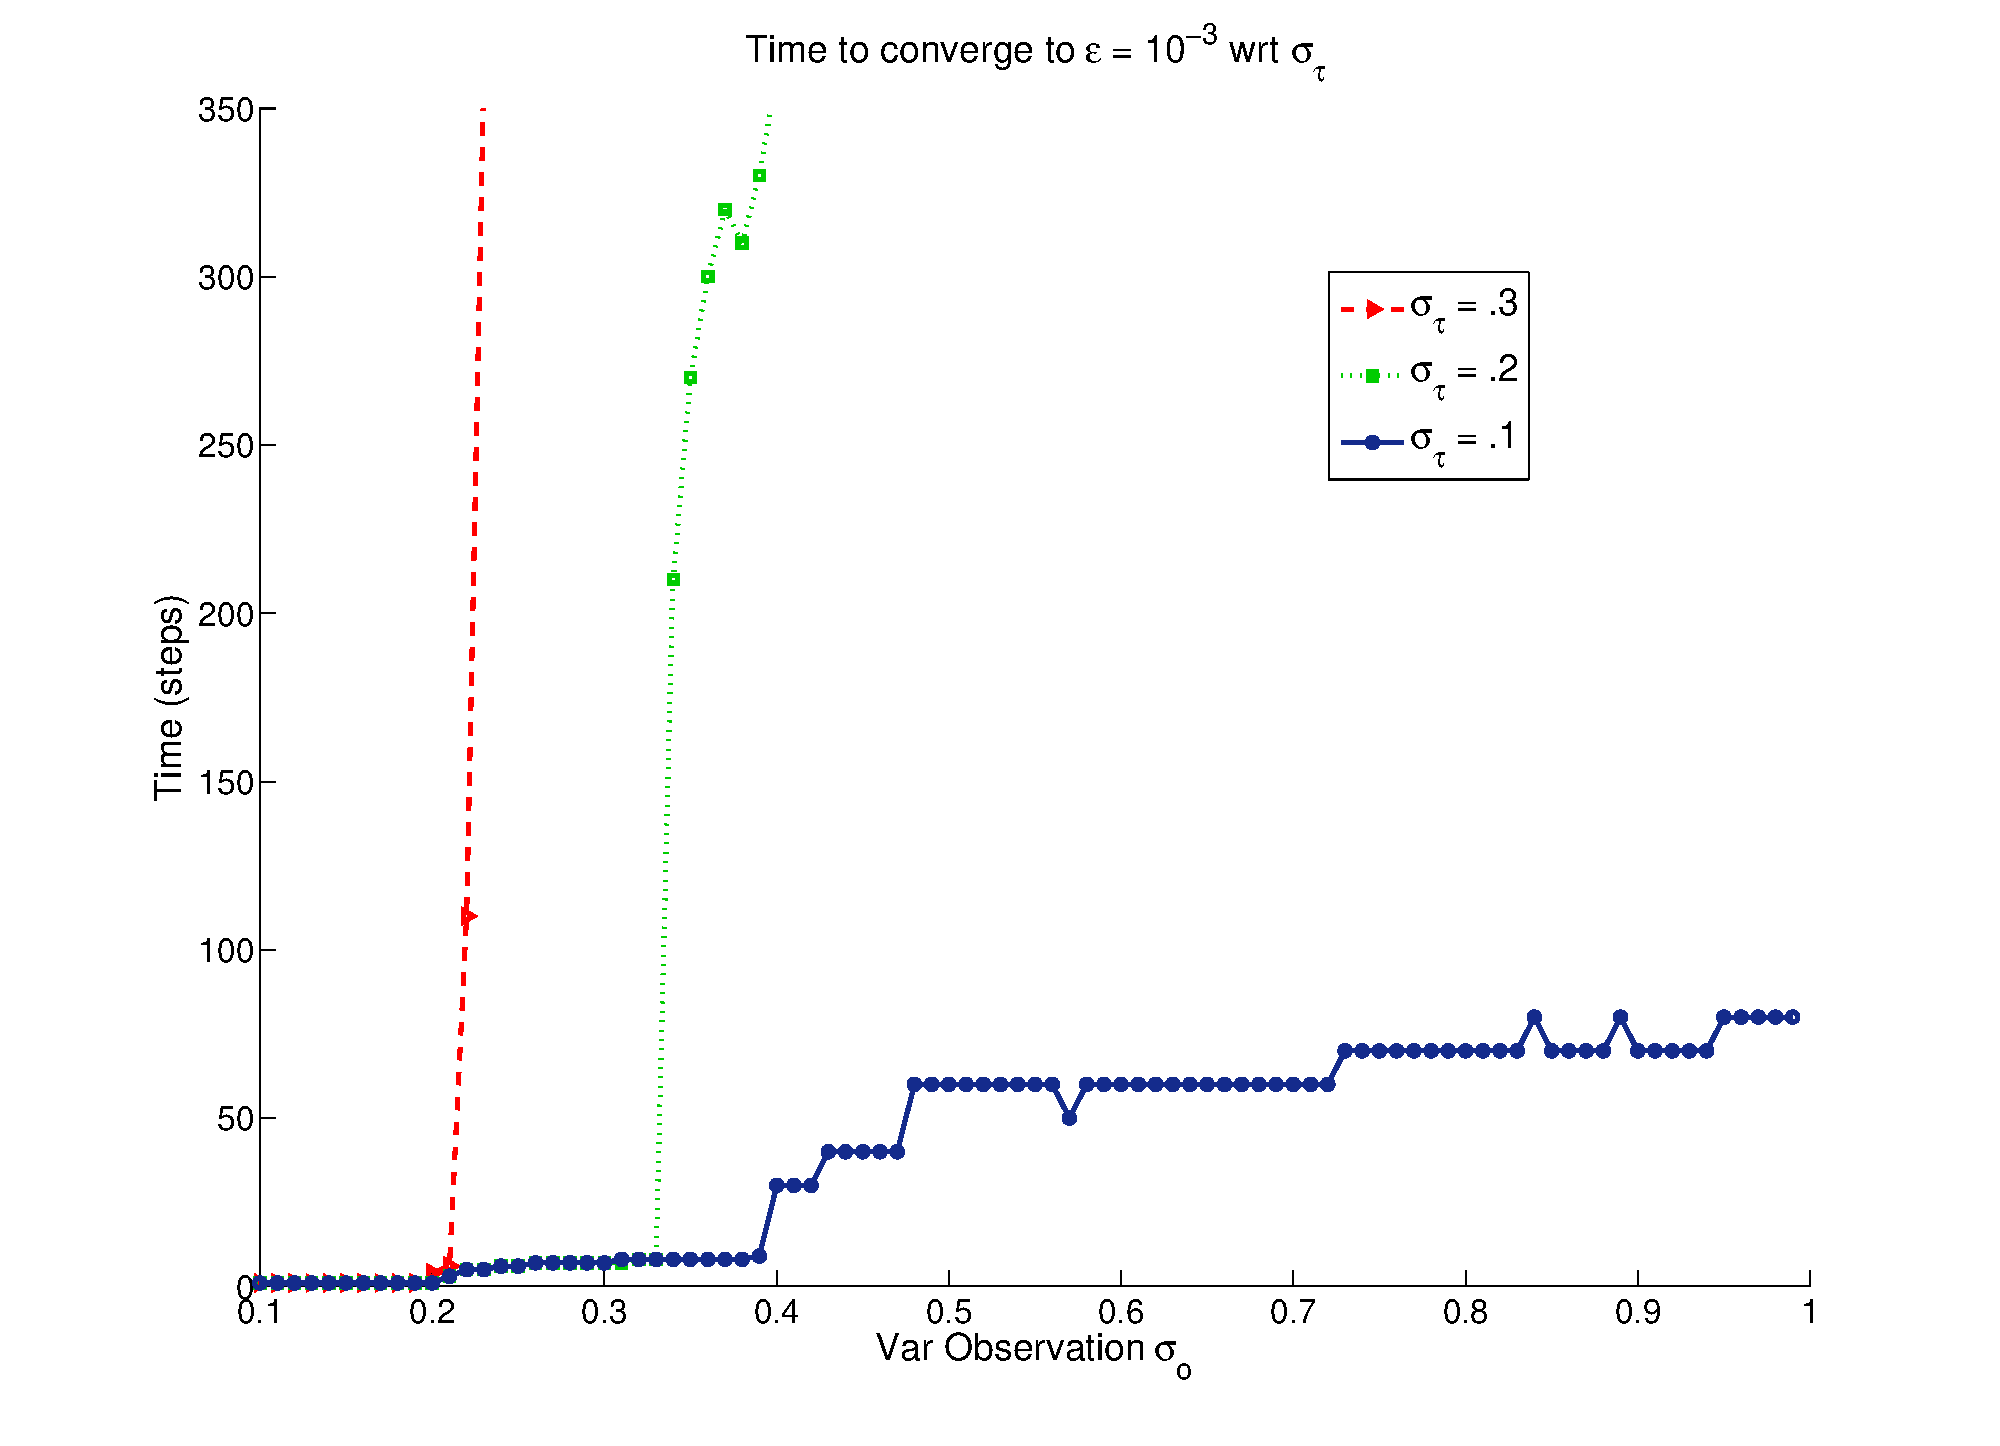
\includegraphics[width=.8\textwidth]{timeToConvZeroVarOnTra3}
%    \begin{tikzpicture}[overlay]
%    \draw[|-latex] (-6.1,2) -- (-6.3,2) -- (-6.4,1.5) node[at start,right,above] {Time = 60 steps};
%    \draw[dashed] (-6.4,1.5) -- (-6.4,.62);
%    %\fill (-4.4,1.5) circle (1pt);
%    %\fill (-4.4,.62) circle (1pt);
%    \end{tikzpicture}
%  \caption[Temps minimal de convergence de l'entropie d'estimation avec politique al�atoire.]{Temps minimal de convergence de l'entropie d'estimation avec politique al�atoire pour diff�rentes variances sur la transition $\sigma_\tau$ et diff�rentes variance sur l'observation $\sigma_o$.}\label{afig:ConvTime}
%\end{figure}

\begin{figure}[h!t]
  \centering
  \subfigure[After 1 step]{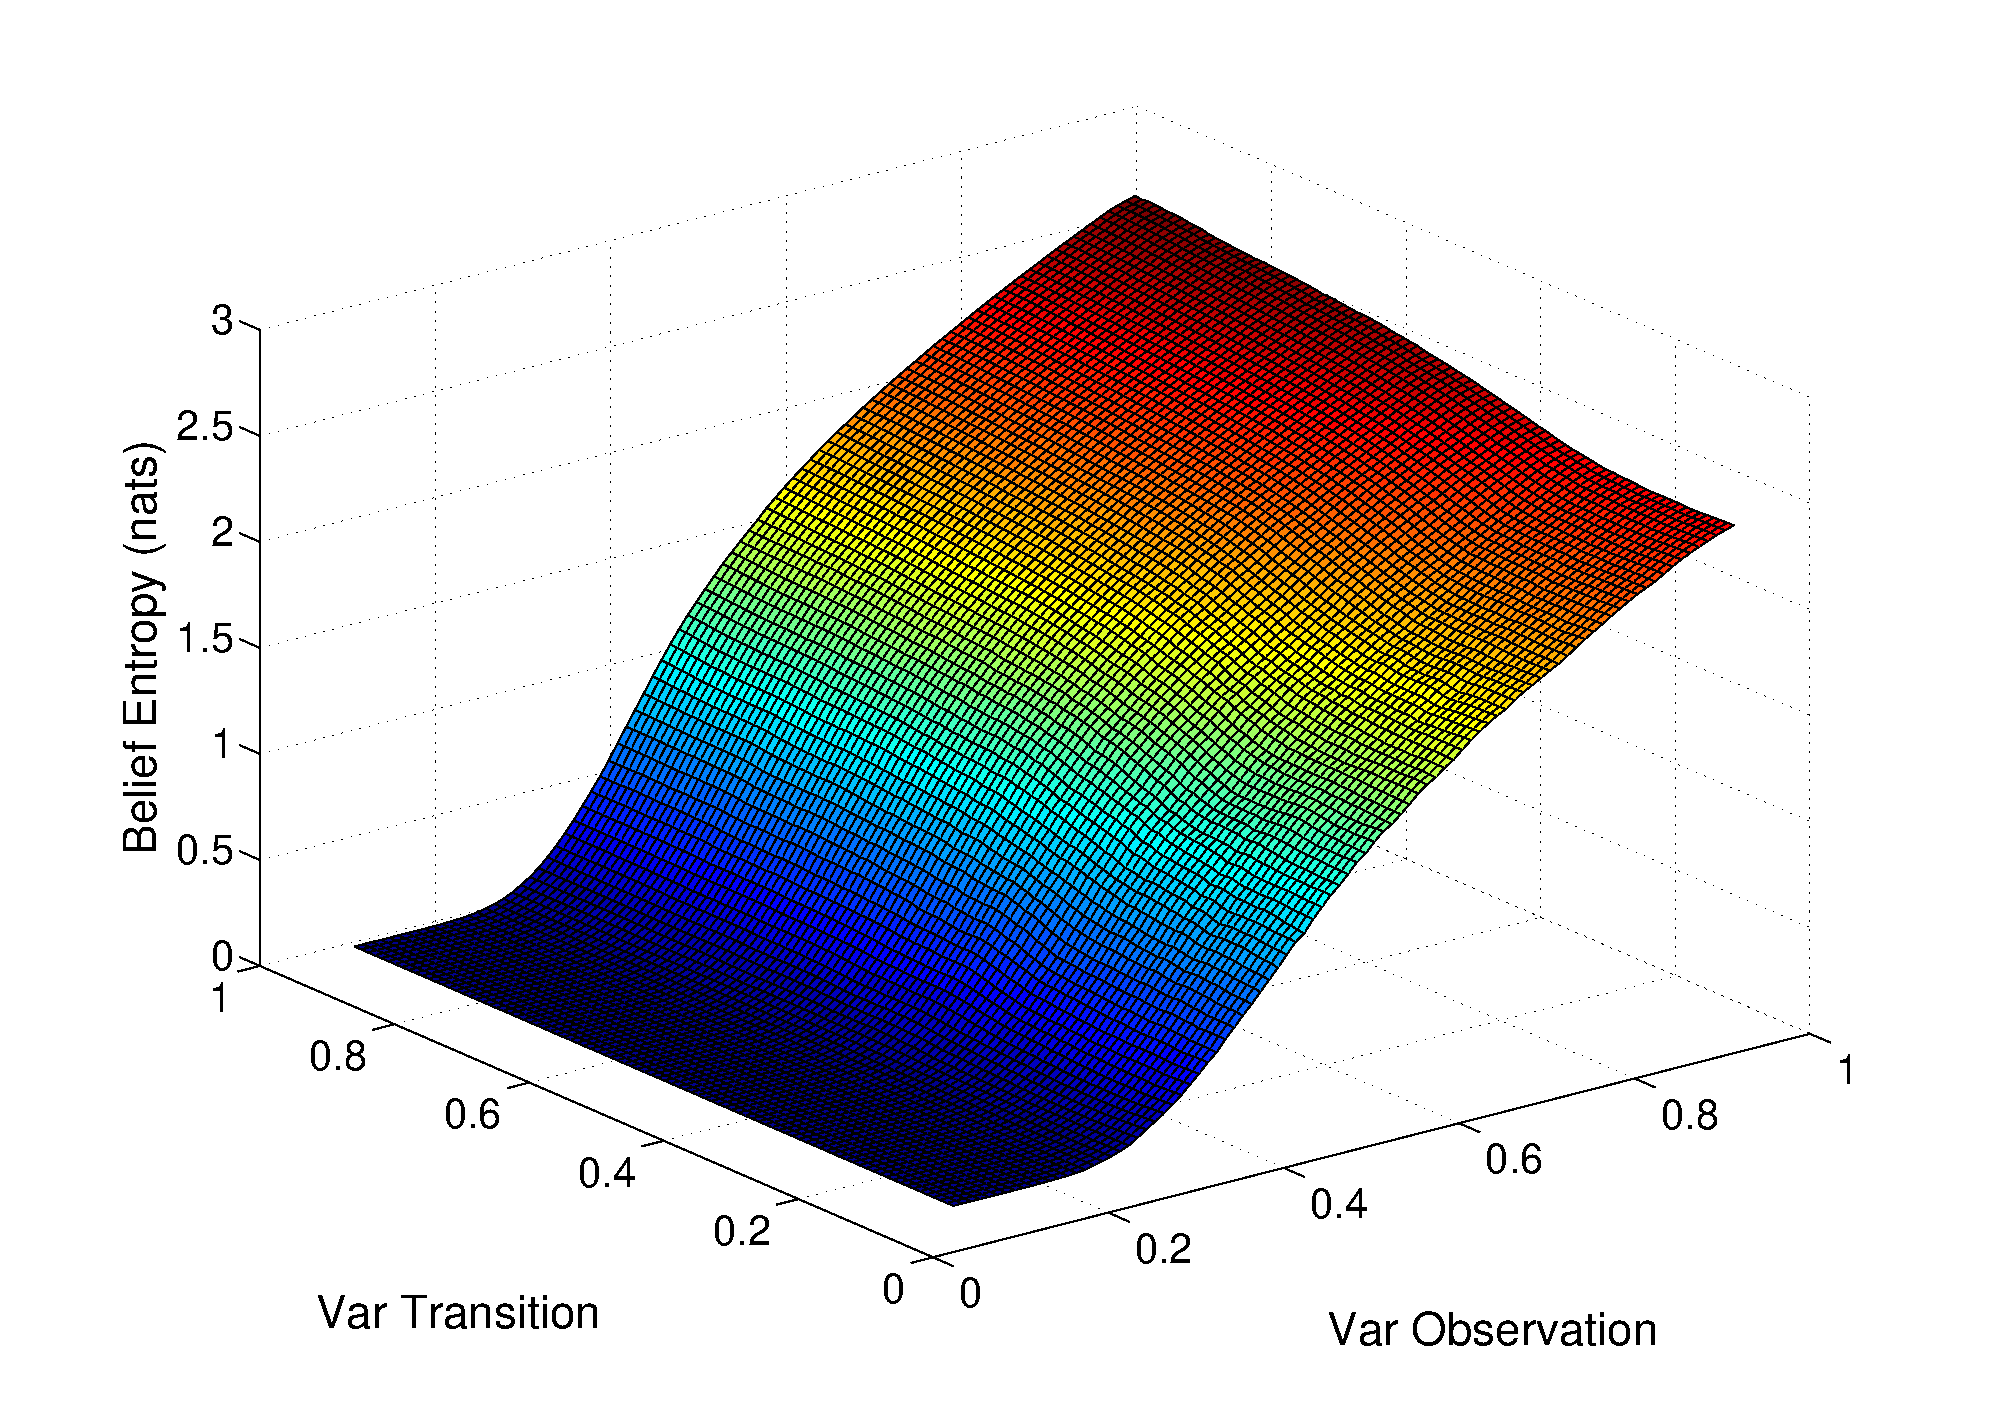
\includegraphics[width=.48\textwidth]{belEnt1}\label{afig:belEnt1}}
  \subfigure[After 5 steps]{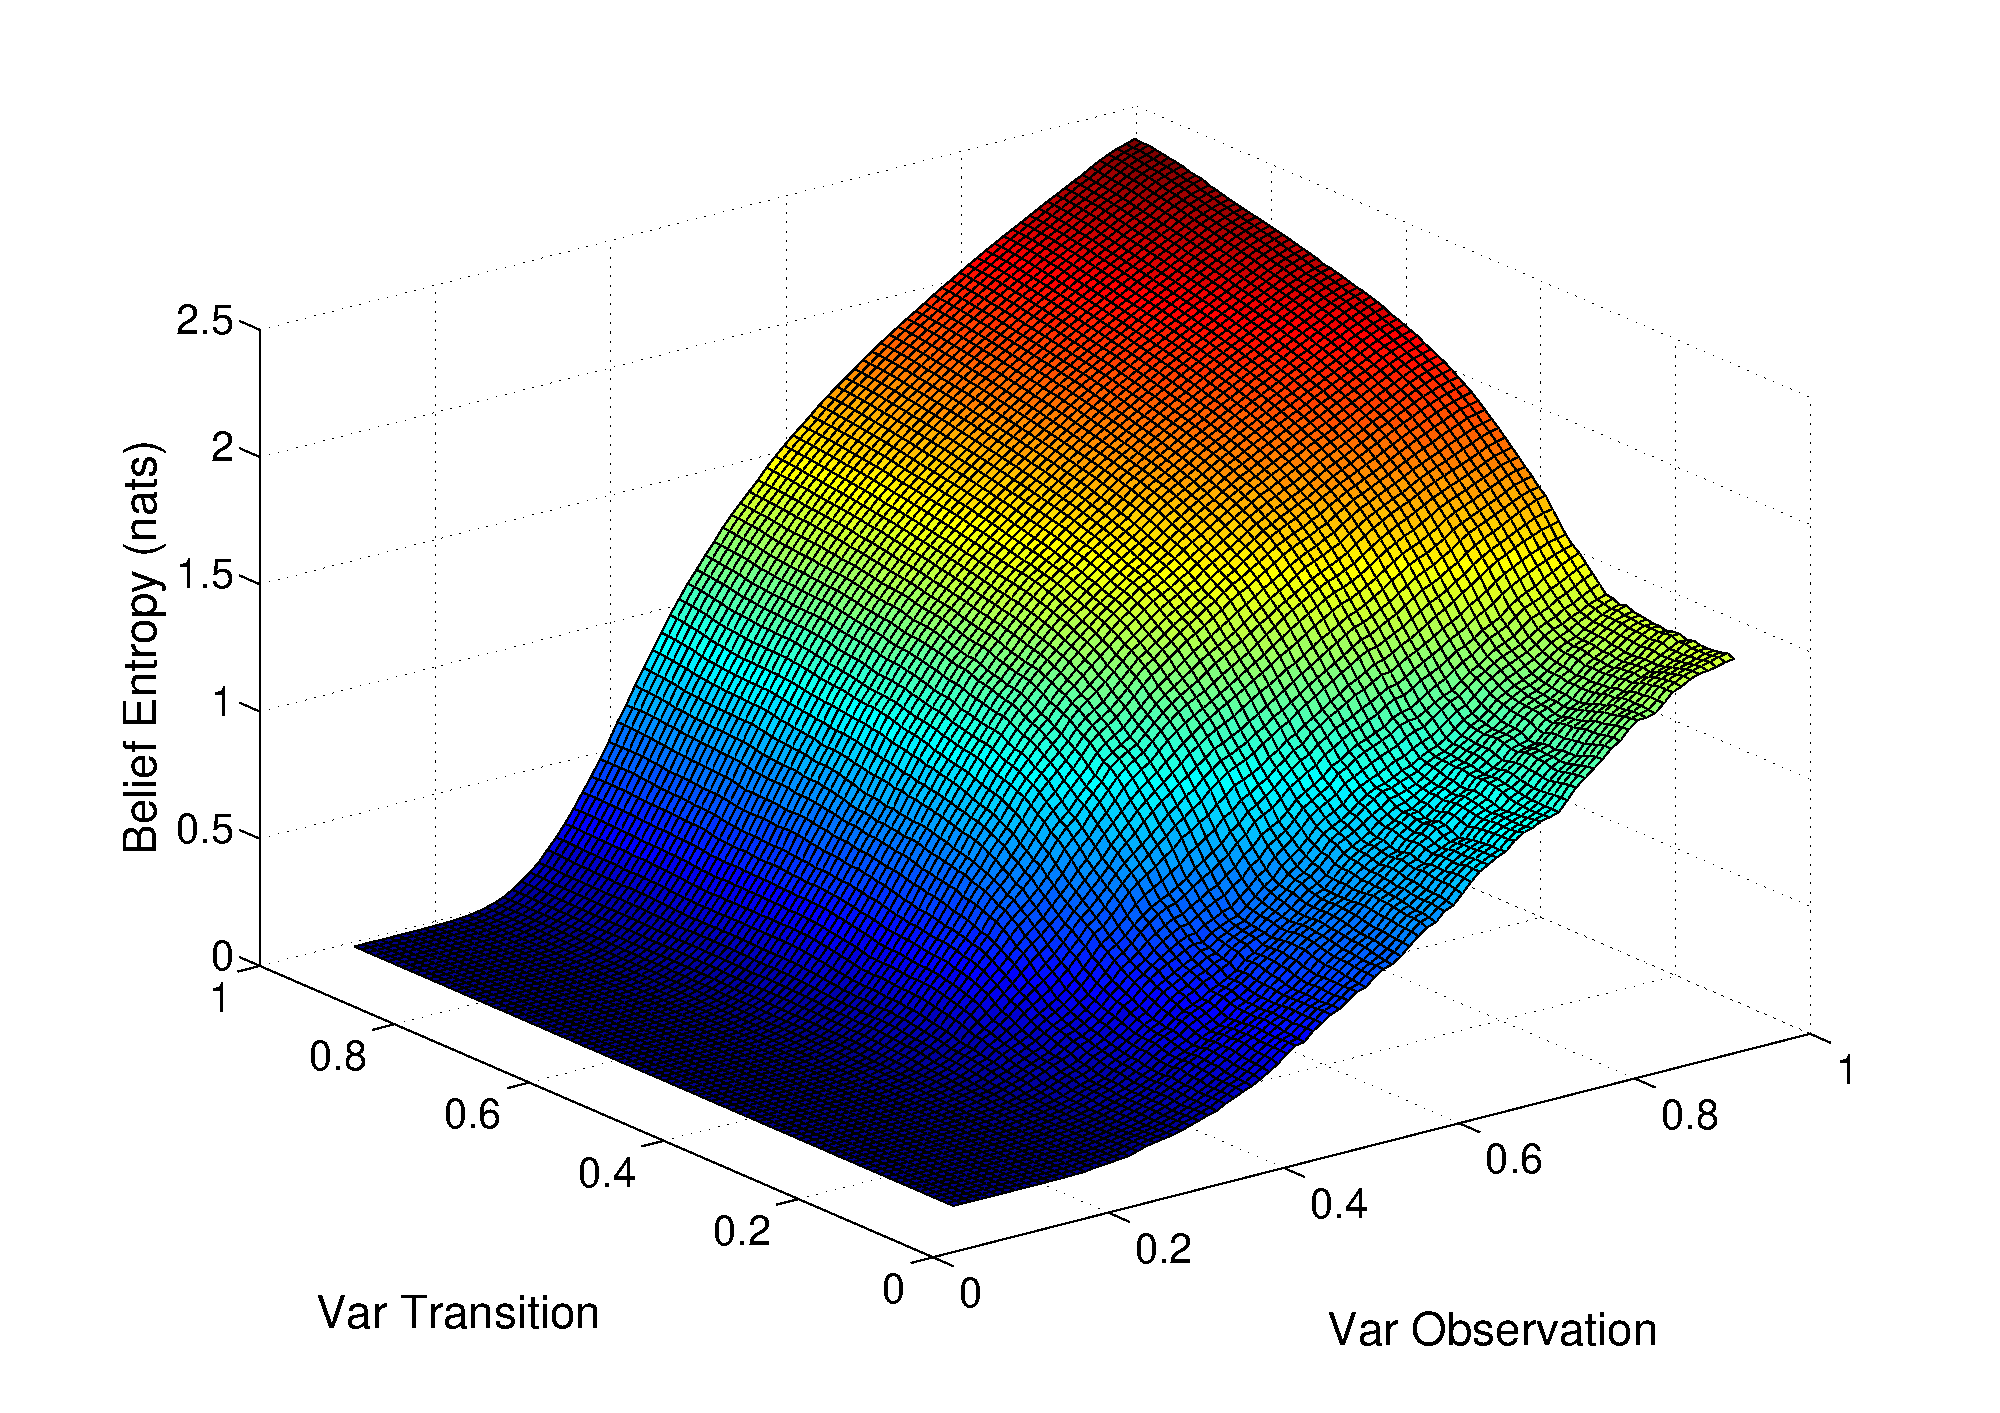
\includegraphics[width=.48\textwidth]{belEnt5}\label{afig:belEnt5}}
  \subfigure[After 8 steps]{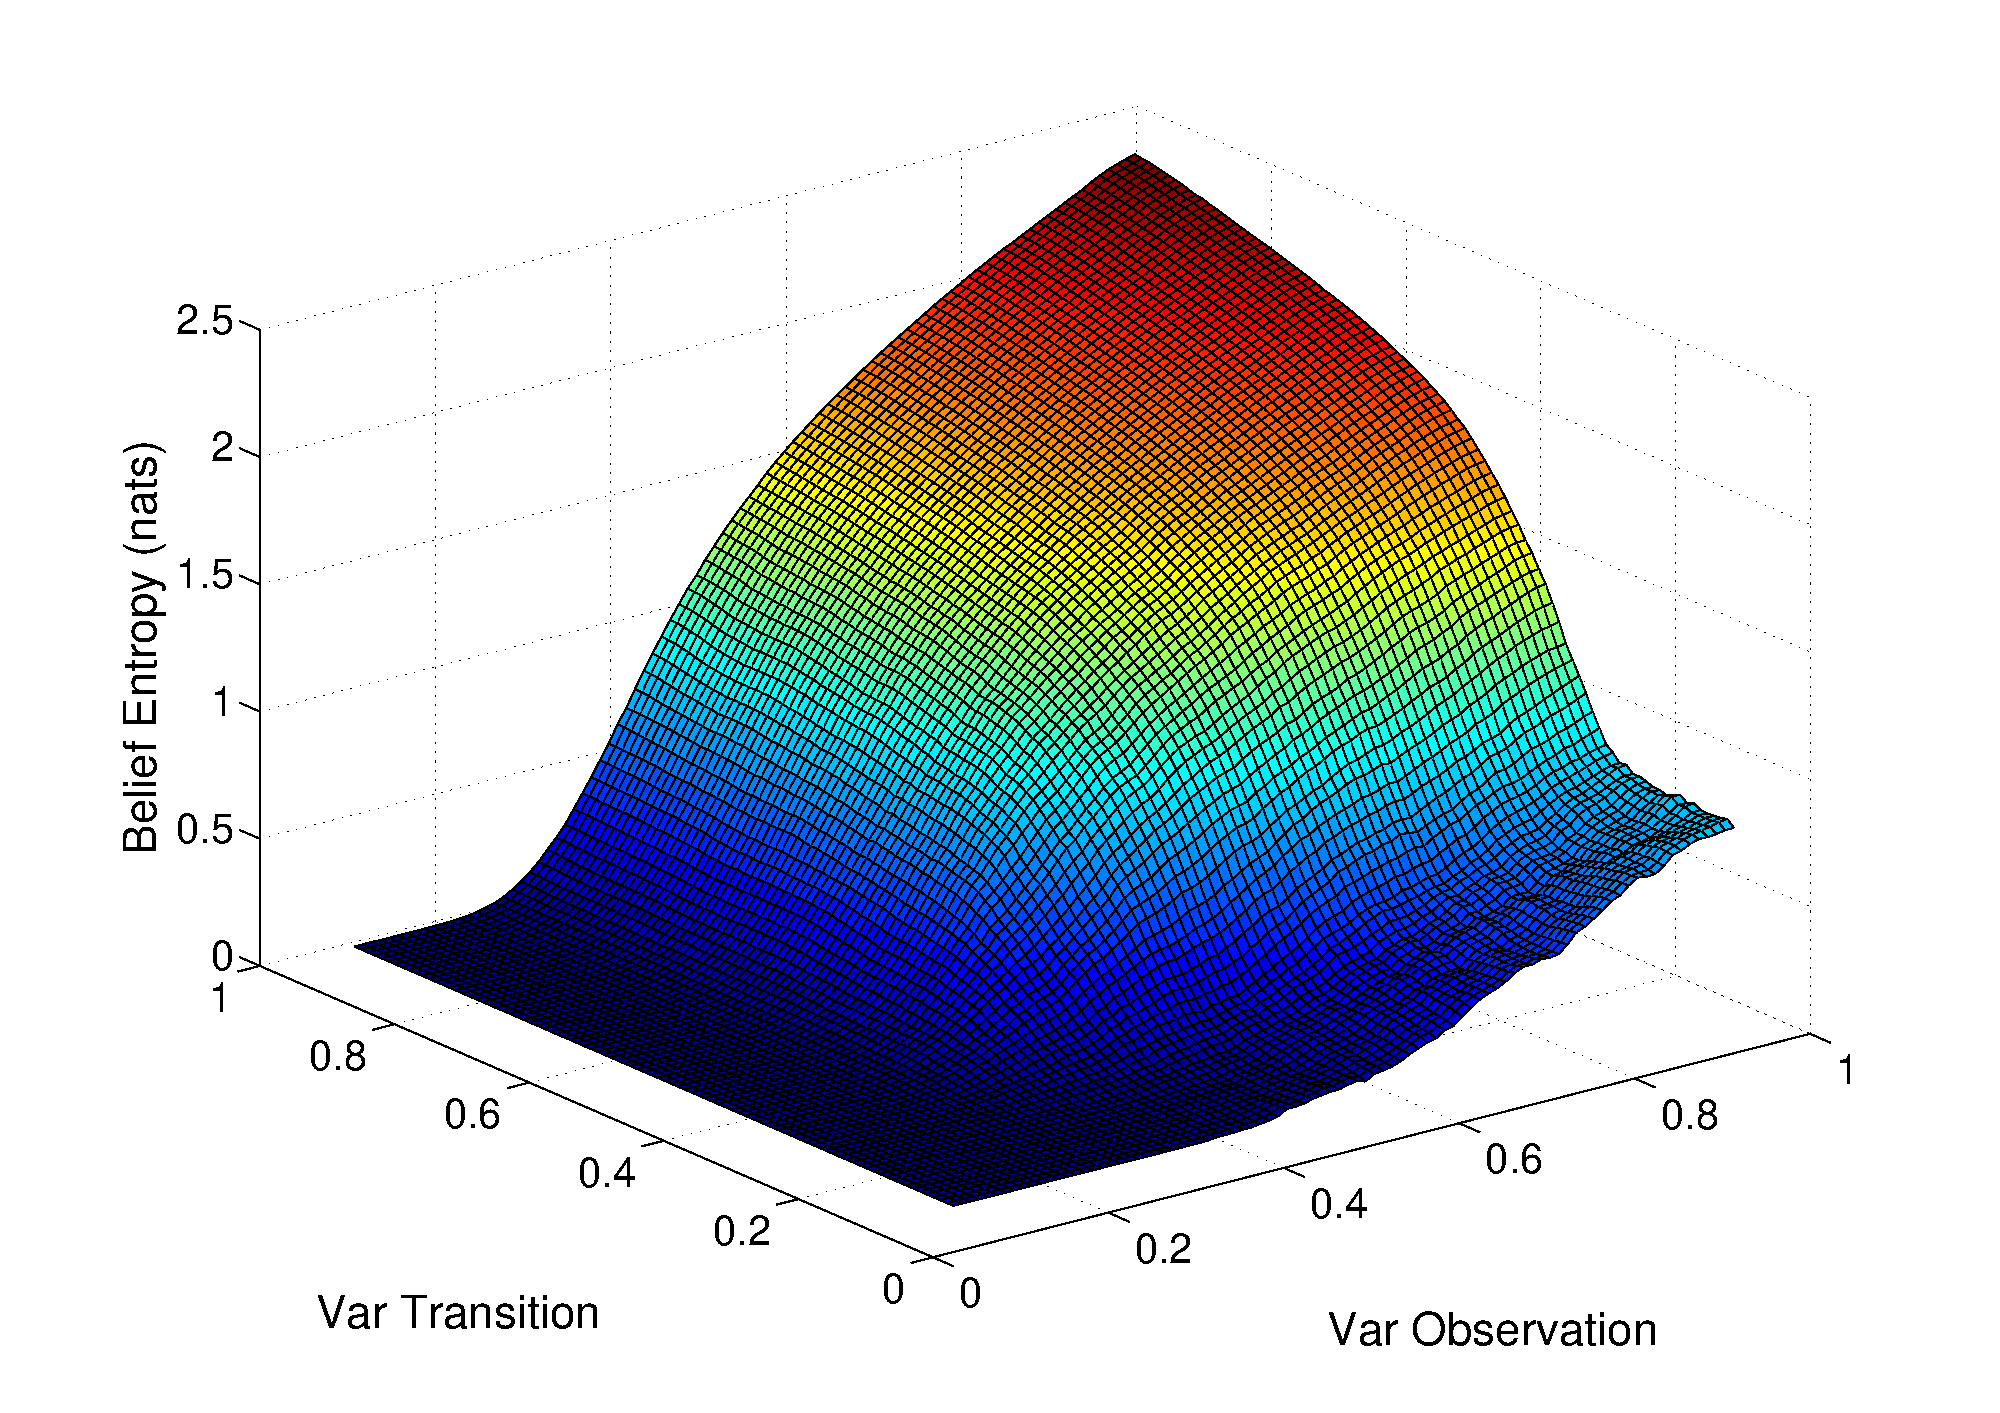
\includegraphics[width=.48\textwidth]{belEnt8}\label{afig:belEnt8}}
  \subfigure[After 50 steps]{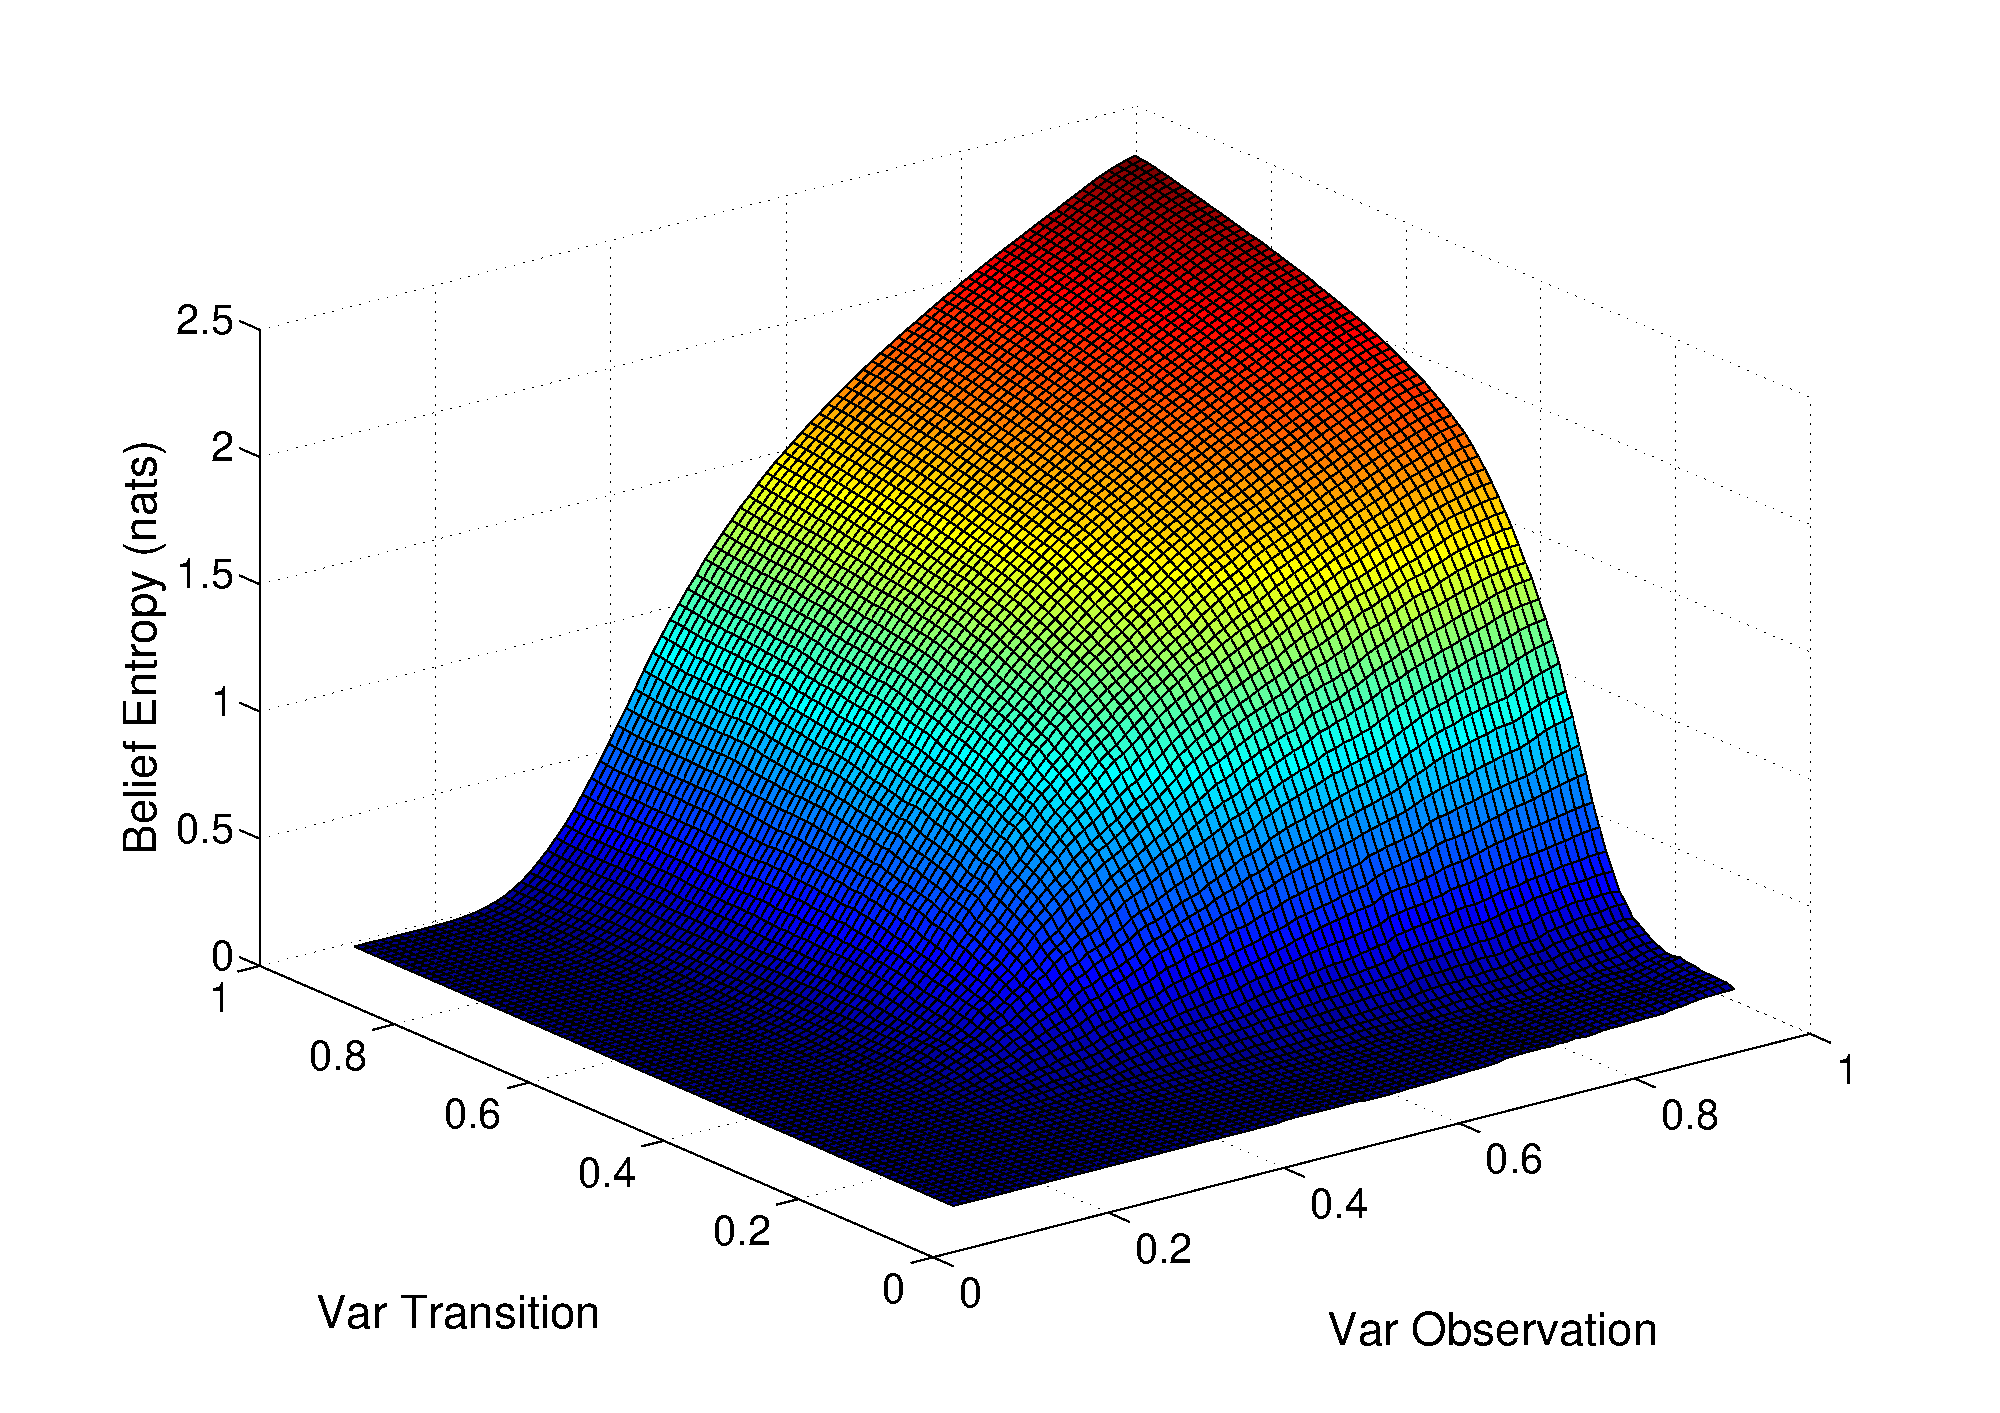
\includegraphics[width=.48\textwidth]{belEnt50}\label{afig:belEnt50}}
  \caption[�tude de la variation de l'entropie pour diff�rentes valeurs de bruits.]{�tude de la variation de l'entropie pour diff�rents valeurs de bruits sur la transition et l'observation.}\label{afig:bee}
\end{figure}

En fait, la figure~\ref{afig:ent3000} montre la convergence de l'entropie d'estimation apr�s avoir suivi une politique al�atoire pendant trois milles �tapes. Ces r�sultats montrent qu'apr�s un certain seuil sur l'erreur de transition (sur la figure entre 0.2 et 0.3), l'entropie de l'�tat de croyance ne peut �tre r�duite plus. Ce seuil survient en fait lorsque la transition n'est plus d�terministe puisqu'au-del� de 0.3 l'erreur sur la transition devient sup�rieure au milli�me comme nous l'avons vu dans la figure~\ref{afig:err}.

Un autre r�sultat int�ressant survient �galement lorsqu'une politique d�terministe est utilis�e plut�t qu'une politique al�atoire (par exemple lorsque le robot cherche � se rendre � une position donn�e et � y rester). Les r�sultats exp�rimentaux de la figure~\ref{afig:ConvTimeDet} montrent en effet que dans ce cas la convergence  est plus rapide pour des valeurs identiques de variances. Par exemple, la figure~\ref{afig:ConvTime} montre qu'il faut au minimum 60 �tapes pour converger lorsque la variance sur l'observation est de 0.5 et que l'on suit une politique al�atoire, alors que ce temps est rarement atteint -- m�me avec une variance de~1 -- lorsqu'une politique d�terministe est utilis�e. Ce r�sultat s'explique tr�s simplement par le fait qu'une politique stochastique induit n�cessairement un taux d'entropie suppl�mentaire sur la cha�ne de Markov sous-jacente. Il convient alors de n'utiliser que des politiques d�terministes lorsque l'on cherche � r�colter de l'information sur l'�tat sous-jacent du syst�me.

\begin{figure}[h!t]
  \centering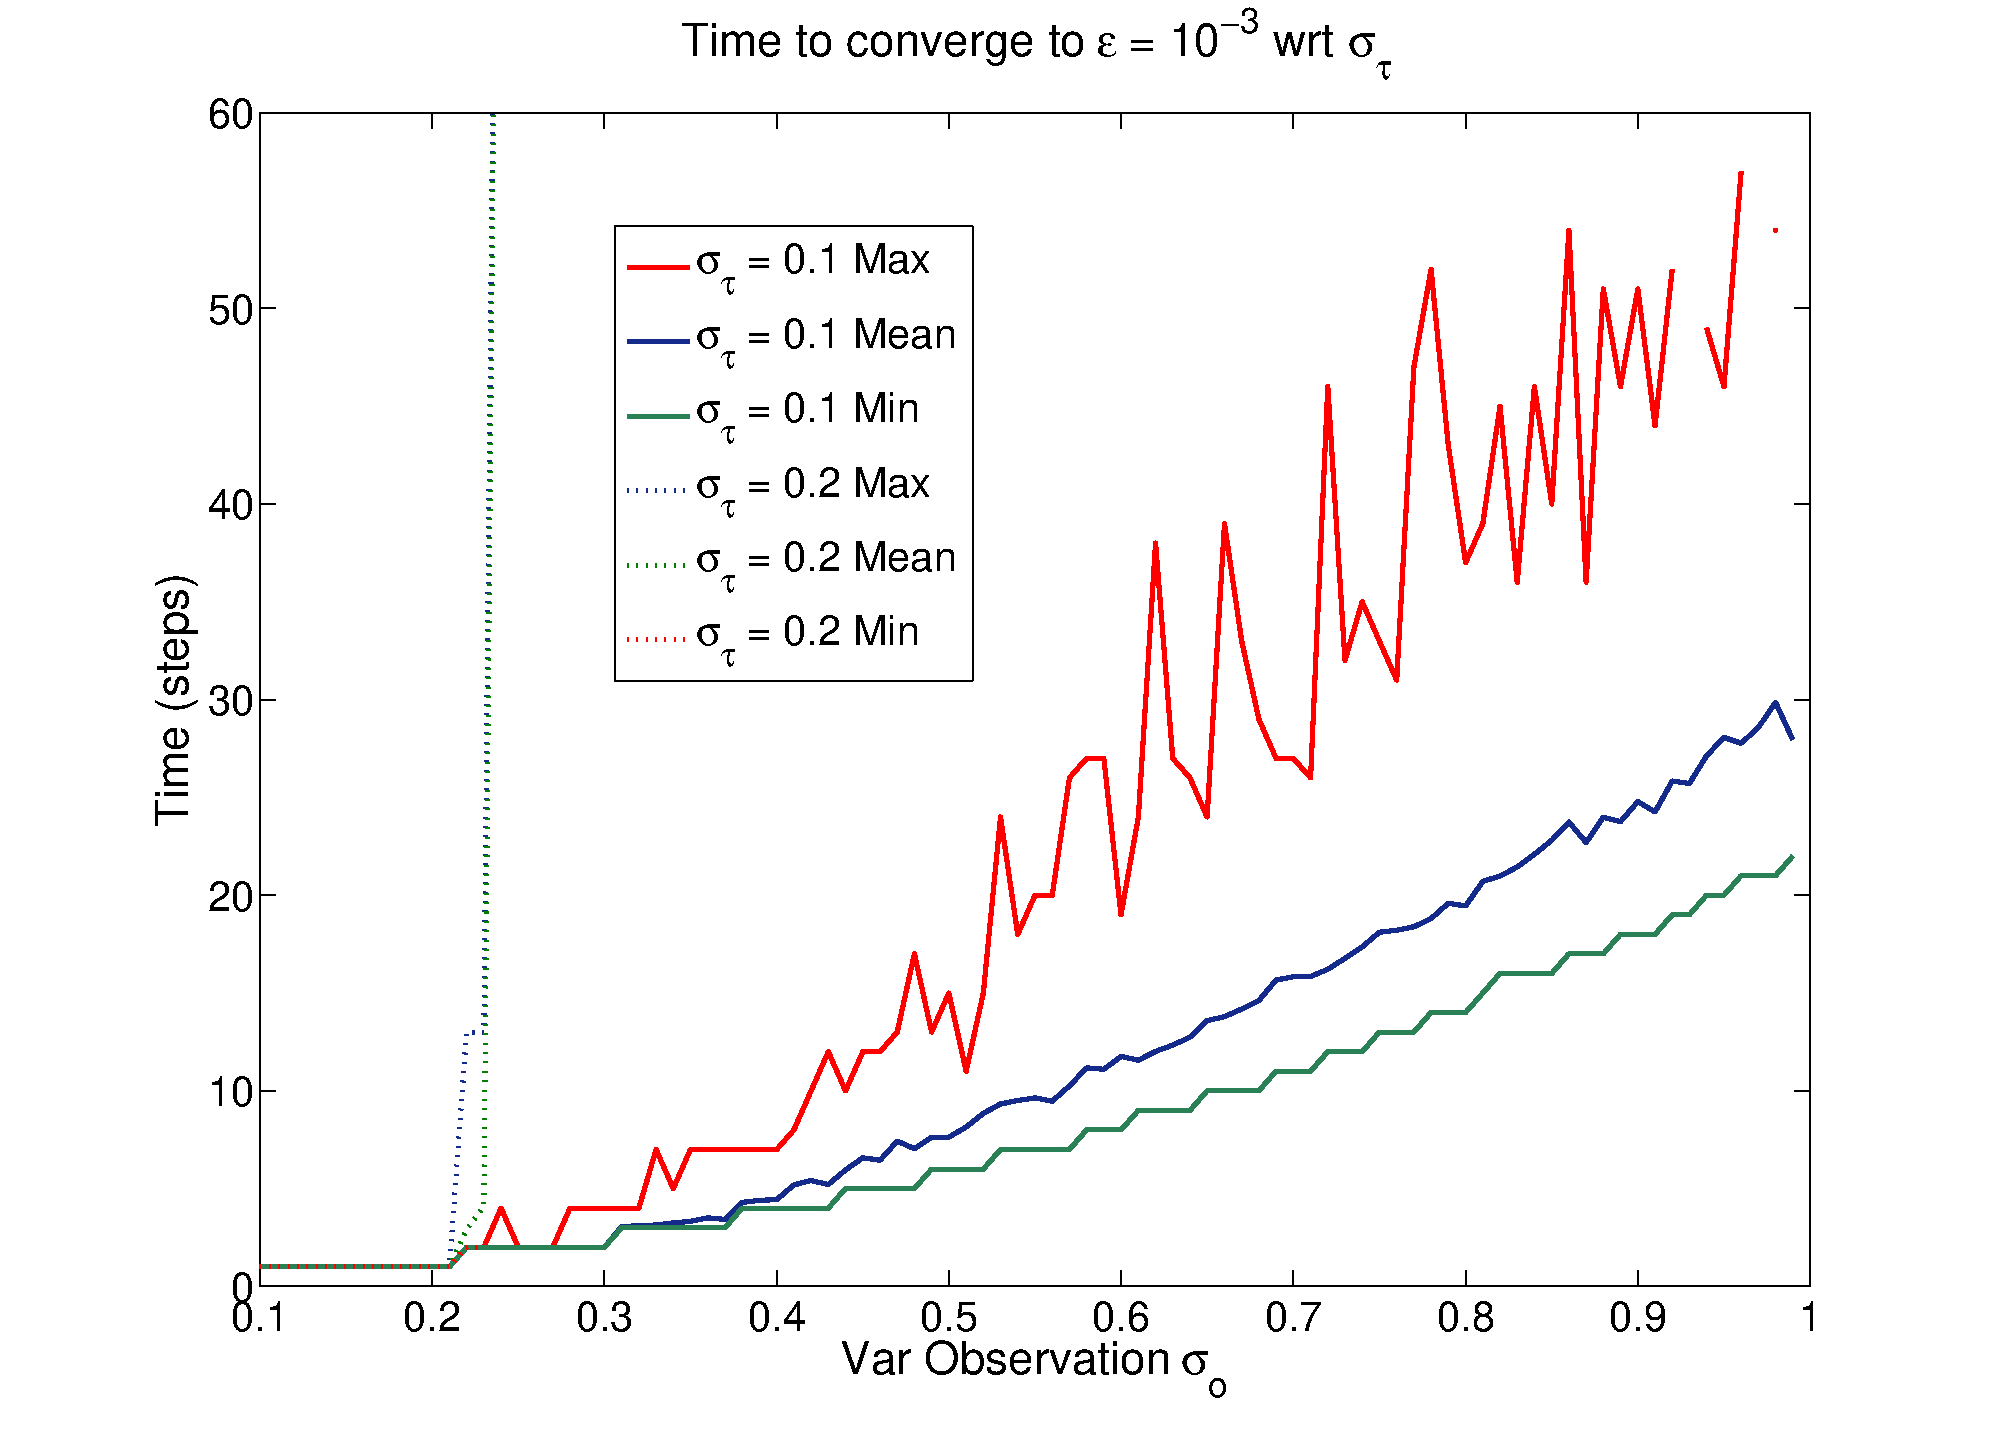
\includegraphics[width=.8\textwidth]{timeToConvZeroVarOnTra4_2}
  \caption[Temps de convergence de l'entropie d'estimation lorsque l'agent suit une politique d�terministe.]{Temps de convergence de l'entropie d'estimation pour des variances sur la transition de $\sigma_\tau =0.1$ et $\sigma_\tau =0.2$ en fonction de la variance sur l'observation $\sigma_o$ lorsque l'agent suit une politique d�terministe. La moyenne, le minimum et le maximum sont calcul�s sur 100 simulations.}\label{afig:ConvTimeDet}
\end{figure}

Finalement, ces r�sultats pr�liminaires ont conduit aux r�sultats th�oriques exprim�s un peu plus haut dans ce chapitre. Il serait extr�mement int�ressant d'�tudier plus avant la th�orie de l'information dans certaines cha�nes de Markov sp�cifiques (et non d�terministes) o� le taux d'entropie instantan� peut-�tre born� sup�rieurement, induisant ainsi une convergence assur�e de l'entropie d'estimation vers 0.

Voyons maintenant l'extension aux probl�mes multiagents de ces mod�les � observation quasi-d�terministe et � transition d�terministe.

\section{\pac{qDet-pomdp}s multiagents}

L'extension du cas monoagent au cas multiagent se fait de mani�re directe en consid�rant un ensemble d'agents $\alpha$ o� chaque agent $i$ poss�de maintenant son ensemble propre d'actions $\Act_i$ et d'observations $\Omega_i$ et o� l'ensemble des actions jointes $\JAct$ est le produit cart�sien des ensembles des actions de tous les agents. Les fonctions de transitions sont ainsi d�finies sur l'ensemble des actions jointes et les conditions requises d'observation minimale sont maintenant d�finies pour toutes les actions jointes $\ba$ dans $\JAct$:

\begin{definition}\label{def:qdetdecpomdp}
Un Processus D�cisionnel de Markov Partiellement Observable D�centralis� Quasi-D�terministe (\qdetdecpomdp) est un tuple $\la \Sta,$ $\{\Act_i\}_{i\in\alpha},$ $\Omega,$ $\Tra,$ $\Obs,$ $\Rew,$ $\gamma,$ $\bel^0 \ra$, o�:%\\
\begin{itemize}
\item $\Sta$ est un ensemble fini d'\emph{�tats} $s \in \Sta$;
\item $\Act_i$ est un ensemble fini d'\emph{actions} $a \in \Act_i$ pour chaque agent $i\in\alpha$ et $\ba \in\JAct$ denote une action jointe de tous les agents;
\item$\Tra(s,\ba,s'): \Sta \times \JAct \times \Sta \mapsto \{0,1\}$ est la \emph{fonction d�terministe de transition} du syst�me de l'�tat $s$ vers l'�tat $s'$ apr�s l'ex�cution de l'action jointe $\ba$;
\item $\Rew(s,\ba): \Sta \times \JAct \mapsto \mathds{R}$ est la \emph{r�compense} produite par le syst�me lorsque l'action jointe $\ba$ est ex�cut�e dans l'�tat $s$,
\item $\Omega_i$ est un ensemble fini d'observations $o \in \Omega_i$ pour chaque agent $i$ et $\bo \in \JObs$ denote une observation jointe de tous les agents,
\item $\Obs(\bz,\ba,s'): \JObs \times \JAct \times \Sta \mapsto [0,1]$ est une \emph{fonction d'observation} qui indique la probabilit� d'obtenir l'observation jointe $\bz$ lorsque le monde arrive dans l'�tat $s'$ apr�s avoir ex�cut� l'action jointe $\ba$;\\
    De plus, $\forall\,s'\in\Sta,\,\ba\in\JAct,\,\exists\,\bz\in\JObs,$ s.t. $\Obs(\bz,\ba,s') \ge \theta > \frac{1}{2}$, i.e. le monde est minimalement observable et la probabilit� d'obtenir une des observations jointe est born�e inf�rieurement par un demi;
\item $\gamma$ est le facteur d'escompte;
\item $\bel^0$ est la connaissance \emph{a priori} sur l'�tat, i.e. l'�tat de croyance initial, suppos� non d�terministe.
\end{itemize}
\end{definition}

On peut �galement �tendre la condition d'observation bijective � plusieurs agents:
\begin{definition}\label{def:decenough-obs}
Un \qdetdecpomdp bijectivement observable est un \qdetdecpomdp o� l'hypoth�se suivante est faite:
\begin{eqnarray*}
&&\forall i\in\alpha, \exists o_1\in\Omega_i,\,\forall \ba\in\JAct,\,\forall s\in\Sta^{o_1},\\
&&\mbox{avec }\Sta^{o_1} = \{s\in\Sta|\exists o_1\in\Omega_i, P(o_1|s,\ba)>P(o|s,\ba),\forall o\ne o_1\},\\
&&\mbox{alors }|\Omega_i|=|\Sta|\mbox{ et }|\Sta^{o_1}| = 1
\end{eqnarray*}
\end{definition}
En d'autres termes, chacun des agents poss�de une observation bijective de l'�tat \emph{complet} du syst�me. Les agents per�oivent ainsi le m�me �tat m�me si ce n'est pas n�cessairement la m�me observation qui est re�ue � chaque �tape par tous les agents. Cette hypoth�se est relativement plus forte que dans le cas monoagent pour deux raisons principales:
\begin{itemize}
\item Les agents peuvent n'avoir qu'une vue locale de leur environnement et donc ne pas percevoir ce que per�oivent d'autres agents vis a vis de l'�tat du syst�me;
\item Les agents peuvent avoir un �tat \emph{interne} qui  leur est propre et que personne d'autre qu'eux ne peut observer, mais qui fait n�cessairement partie de l'�tat global pour une prise de d�cision optimale.
\end{itemize}
En regard de ces deux points, il n'est pas interdit de regarder vers la communication pour r�soudre ces deux probl�mes. La communication permet aux agents de fusionner l'information qu'ils ont sur le monde et de partager leur �tat interne. Bien qu'elle ne soit pas parfaite, on peut n�anmoins assumer qu'elle l'est quasiment au regard des techniques actuelles de correction d'erreur. On peut �galement faire l'hypoth�se que dans la majorit� des probl�mes, la communication est beaucoup plus rapide que la fr�quence des instants de d�cision. Ces points seront plus amplement discut�s dans la section \ref{c4:s:dtc}.

\subsection{R�sultats th�oriques}

Les r�sultats th�oriques valides dans le cas monoagent, peuvent s'�tendre ais�ment au cas multiagent et permettre, dans ce contexte, des gains en complexit� en pire cas encore plus int�ressants. En effet, la o� un gain relatif en espace se faisait par la limitation de l'historique � maintenir pour �tre certain de l'�tat sous-jacent du syst�me, il est maintenant possible non seulement de borner son propre historique � m�moriser, mais �galement l'historique de tous les autres agents du syst�me.

Pour rappel, les \decpomdps sont r�put�s pour �tre particuli�rement difficiles � r�soudre optimalement dans le cas � horizon fini (\textsc{nexp}-complet~\citep{BZI.00}) et m�me � approximer~\citep{RGR.03}. En restreignant la mod�lisation aux probl�mes quasi-d�terministes avec observabilit� bijective, il est possible de r�duire de beaucoup cette complexit� en pire cas et on peut donc �noncer le corollaire suivant:

\begin{corollary}\label{fixedHorizonQDETDECPOMDP}
Trouver une politique pour un \qdetdecpomdp � horizon infini, sous l'hypoth�se d'observabilit� bijective, qui produit une r�compense escompt�e esp�r�e d'au moins $C$ avec probabilit� $1-\delta$, est \textsc{pspace}.
\end{corollary}
\begin{proof}
Pour montrer que ce probl�me est \textsc{pspace}, l'algorithme suivant donne la politique $\varepsilon$-optimale en espace polyn�mial: Construire l'arbre de tous les historiques possibles � horizon $k$ (possible en espace $\Obs((|\JAct||\JObs|)^k)$), et calculer ensuite pour chaque feuille de l'arbre construit la valeur esp�r�e escompt�e de l'�tat de croyance quasi-d�terministe atteint en utilisant la valeur de la politique optimale du \mmdp sous-jacent. R�tropropager finalement la valeur jusqu'� la racine pour v�rifier que la r�compense $C$ est effectivement obtenue.
\end{proof}
En d'autre termes, trouver une politique optimale pour un \qdetdecpomdp � horizon infini est aussi complexe en pire cas que de r�soudre un \pomdp � horizon fini.

Voyons maintenant un exemple permettant d'illustrer l'utilisation de ce mod�le avant de discuter plus avant les hypoth�ses et les applications d'un tel mod�le.

\subsection{R�sultats exp�rimentaux : application � la lutte contre l'incendie}\label{sect:res:incendie}

Comme le sugg�re la preuve des corollaires~\ref{fixedHorizonQDETPOMDP} et~\ref{fixedHorizonQDETDECPOMDP}, un algorithme pour r�soudre $\varepsilon$-optimalement un probl�me \qdetdecpomdp � horizon infini sous l'hypoth�se d'observabilit� bijective consiste � calculer une politique escompt�e classique pour le probl�me � horizon fini � $k$ �tapes et � utiliser ensuite le \mmdp sous-jacent pour terminer l'ex�cution de la t�che. Un tel algorithme serait la Programmation Dynamique~\citep{HBZ.04} vue au chapitre~\ref{chap:2} par exemple. En pratique cependant, r�soudre un \decpomdp � horizon $k$ -- m�me quasi-d�terministe -- devient extr�mement complexe d�s lors que $k>2$ et une approximation devient n�cessaire. Les r�sultats pr�sent�s ci-apr�s sont donc r�alis�s � partir d'un algorithme d'approximation sur un probl�me de cha�ne de seaux d'eau (cf figure~\ref{fig:fire}).

\begin{figure}[h!tb]
    \centering
    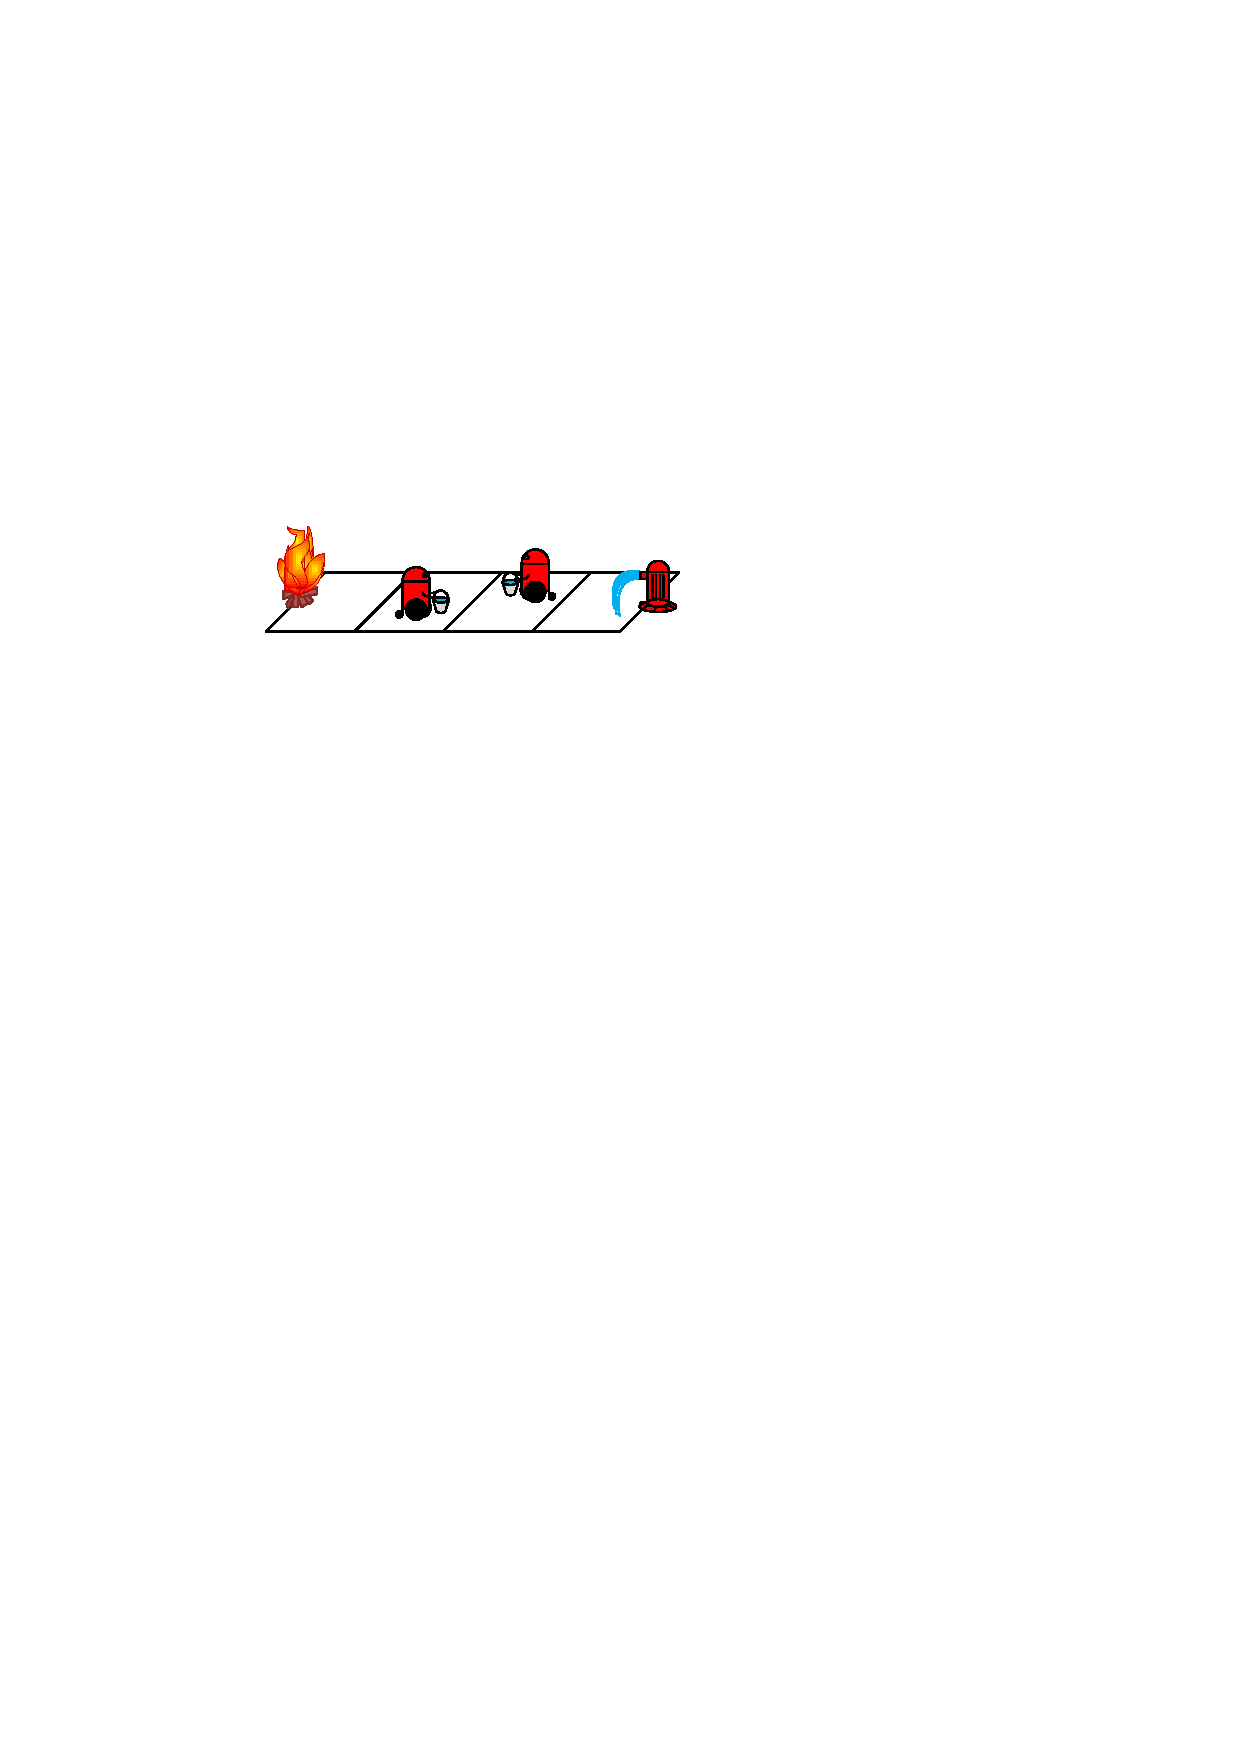
\includegraphics[width=.65\textwidth]{firefight}
  \caption{Le probl�me de la cha�ne de seaux.}\label{fig:fire}
\end{figure}

La version g�n�rale du probl�me de cha�ne de seaux d'eau est comme suit: deux agents sont situ�s sur une grille lin�aire et portent chacun un seau. Ils peuvent aller � \emph{droite} ou � \emph{gauche}, ou encore \emph{jeter de l'eau}, chaque action infligeant une petite p�nalit� de retard ($-0.1$ par agent). D�s qu'un agent se trouve sur la case la plus � droite, le seau se remplit automatiquement avec une probabilit�~$\varphi$. Chaque action de d�placement a �galement une probabilit� $\varphi$ de r�ussir, l'action consistant � jeter de l'eau r�ussissant syst�matiquement. Les agents peuvent s'�changer leurs seaux au travers de la m�me action de jet d'eau. � chaque fois qu'un seau est vid� dans la case la plus � gauche par le biais d'un jet d'eau, une r�compense est obtenue ($1$ par agent). Les agents sont initialement positionn�s al�atoirement sans eau. Les agents sont suppos�s avoir une observation bruit�e de leur position, i.e. ils ont une probabilit� $\theta$ d'observer leur position r�elle et une probabilit� $(1-\theta)\slash 2$ d'observer une des cases adjacentes. Ils re�oivent �galement une communication bruit�e de la position de l'autre agent et de l'�tat de son seau. Puisque le probl�me peut-�tre un probl�me � horizon infini, un facteur d'escompte $\gamma = 0.95$ a �t� utilis�. Dans les exp�rimentations pr�sent�es ci-apr�s, une valeur de $\varphi = 1$ a �t� aussi utilis�e pour l'hypoth�se de transition d�terministe. Lorsque $\varphi = 1$ le nombre d'�tats accessibles est de 49 (7 pour chaque agent) et donc 49 observations peuvent �tre obtenues. Dans le cas bijectif factoris�, le nombre d'observations est seulement de 10 puisque chaque agent a 4 positions plus l'�tat du seau de l'autre agent.

Pour ce probl�me, nous avons utilis� une version adapt�e de l'algorithme \textsc{imbdp}~\citep{SZ.07b} pr�sent�e � la section~\ref{sect:mbdp} de telle sorte qu'il utilise la valeur optimale du \mmdp sous-jacent et inclut �galement le facteur d'escompte. Cet algorithme est d�not� par \textsc{imbdp}$^i$ dans les figures.

Plusieurs simulations ont �t� r�alis�es utilisant diff�rents param�tres. La figure~\ref{fig:res_1} montre la valeur esp�r�e escompt�e de \textsc{imbdp}$^i$ sur le probl�me bijectif classique pour plusieurs valeurs de $\theta$ allant de $0.6$ � $0.95$. Les meilleurs param�tres trouv�s par validation crois�e de \textsc{imbdp}$^i$ sont $maxTree = 5$ et $maxObs = 1$. Augmenter ces param�tres n'am�liore pas significativement la valeur esp�r�e escompt�e, mais d�t�riore significativement les performances spatiales et temporelles de l'algorithme. Comme l'on pouvait le pr�voir, � mesure que $\theta$ approche de un, l'horizon de planification n�cessaire diminue jusqu'� deux et la valeur de la politique � horizon infini s'approche de la valeur de la politique optimale du \mmdp sous-jacent.

\begin{figure}[h!tb]
    \centering
    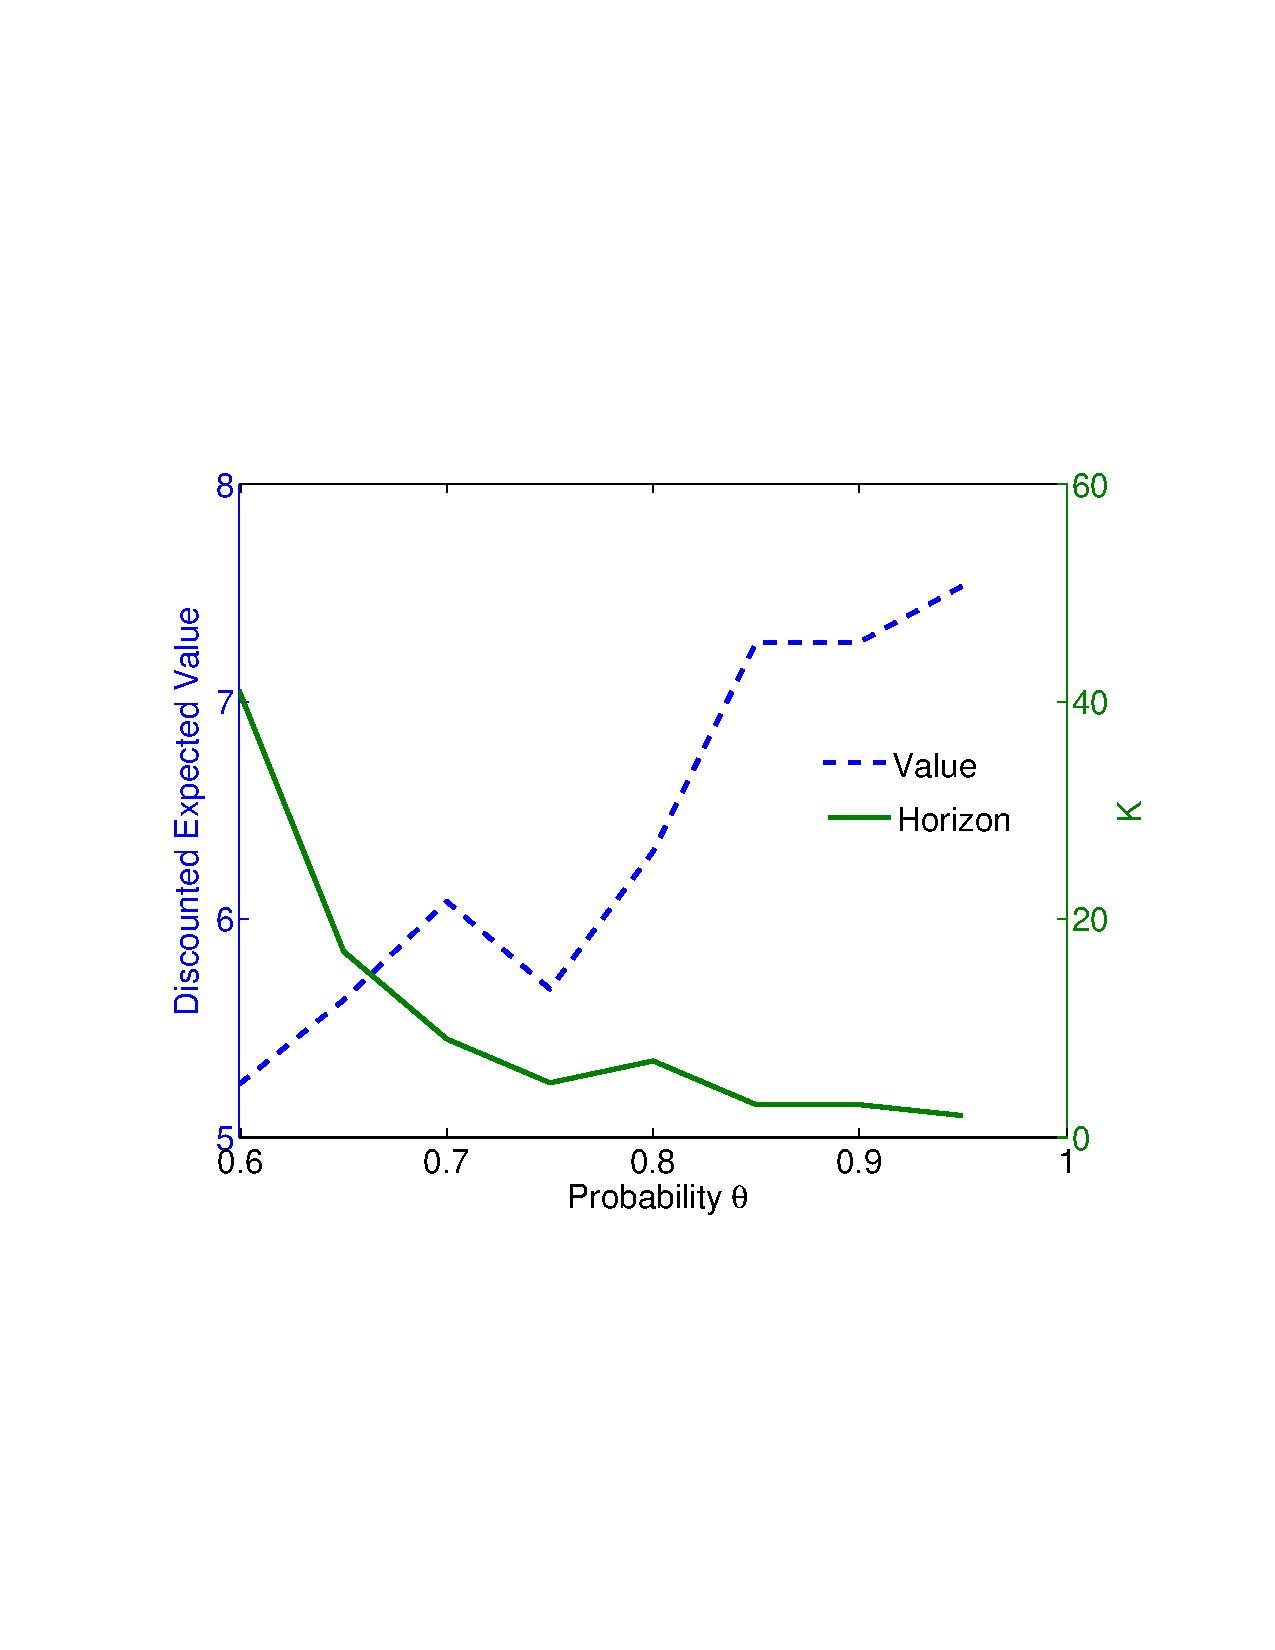
\includegraphics[width=.65\textwidth]{detdec_2}
  \caption{Valeur esp�r�e escompt�e et horizon esp�r� pour diff�rentes valeurs de $\theta$.}\label{fig:res_1}
\end{figure}

La figure~\ref{fig:res_2} montre les valeurs esp�r�es escompt�es pour $\theta = 0.8$ sur plusieurs valeurs de l'horizon allant de 3 � 101 montrant que l'algorithme tend vers la valeur � horizon infinie trouv�e pr�c�demment. L'algorithme \textsc{imbdp} standard a �t� utilis� avec les m�mes param�tres que ci-dessus ($maxTree = 5$ et $maxObs = 1$).

\begin{figure}[h!tb]
    \centering
    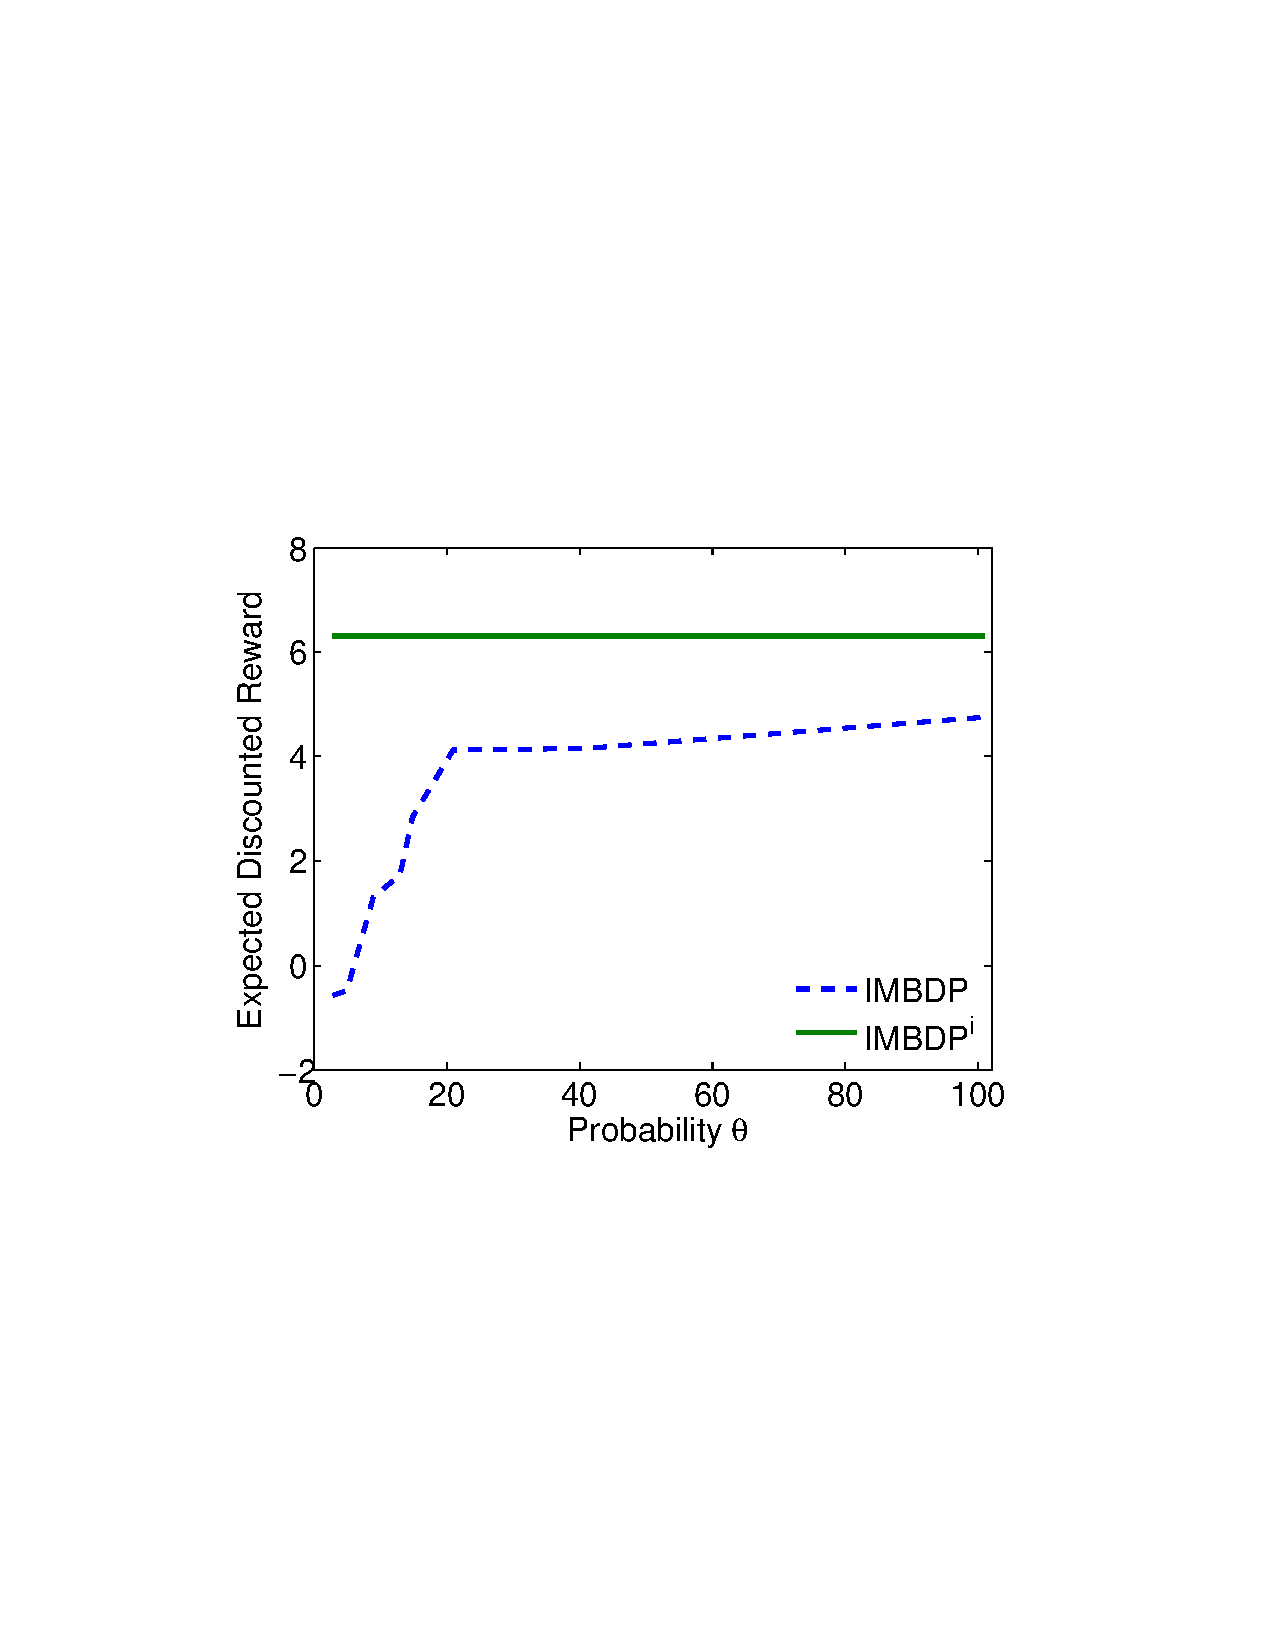
\includegraphics[width=.65\textwidth]{detdec22}
  \caption{Valeur esp�r�e escompt�e � horizon fini pour diff�rentes valeurs d'horizons.}\label{fig:res_2}
\end{figure}
%\begin{figure*}[h!tb]
%\centering
%  \begin{minipage}{.48\textwidth}\centering
%    \centering
%    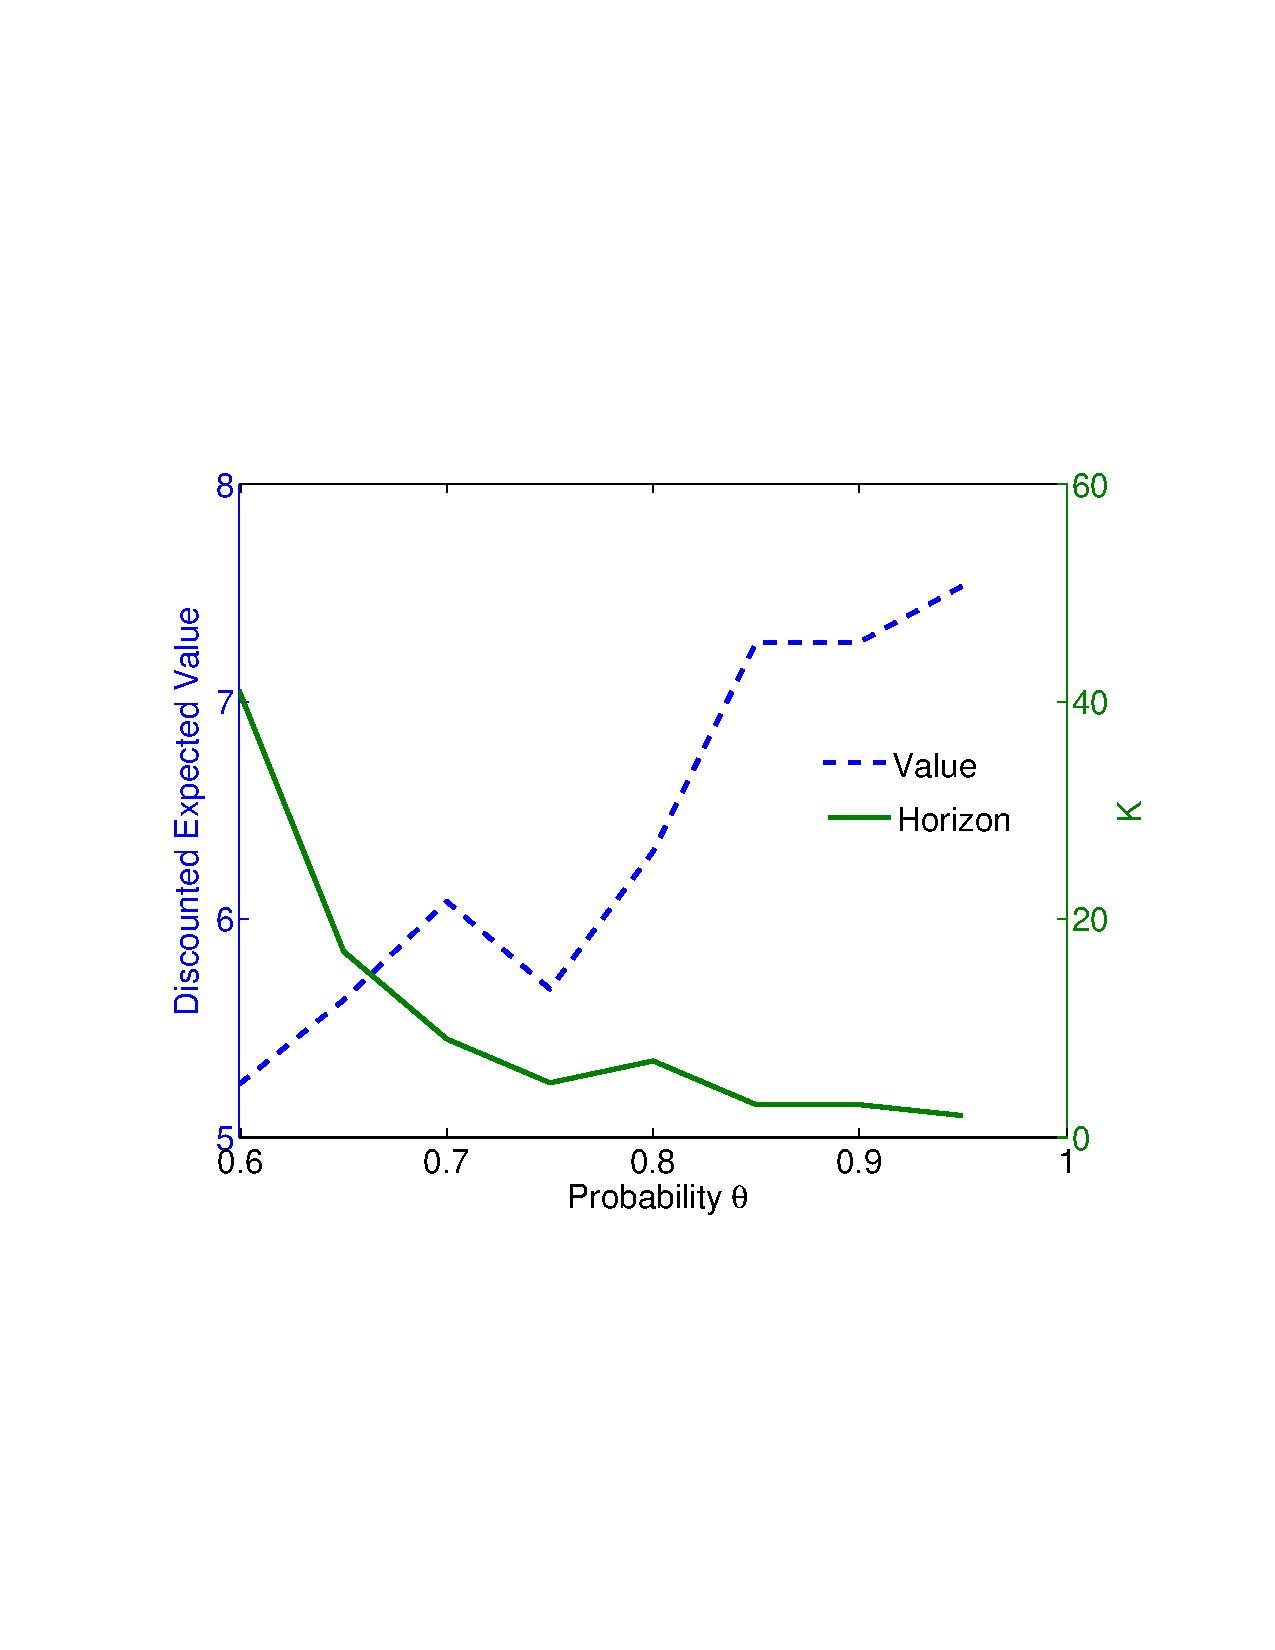
\includegraphics[width=\textwidth]{detdec_2}
%  \caption{Valeur esp�r�e escompt�e et horizon esp�r� pour diff�rentes valeur de $\theta$.}\label{fig:res_1}
%  \end{minipage}
%  ~
%  \begin{minipage}{.48\textwidth}\centering
%    \centering
%    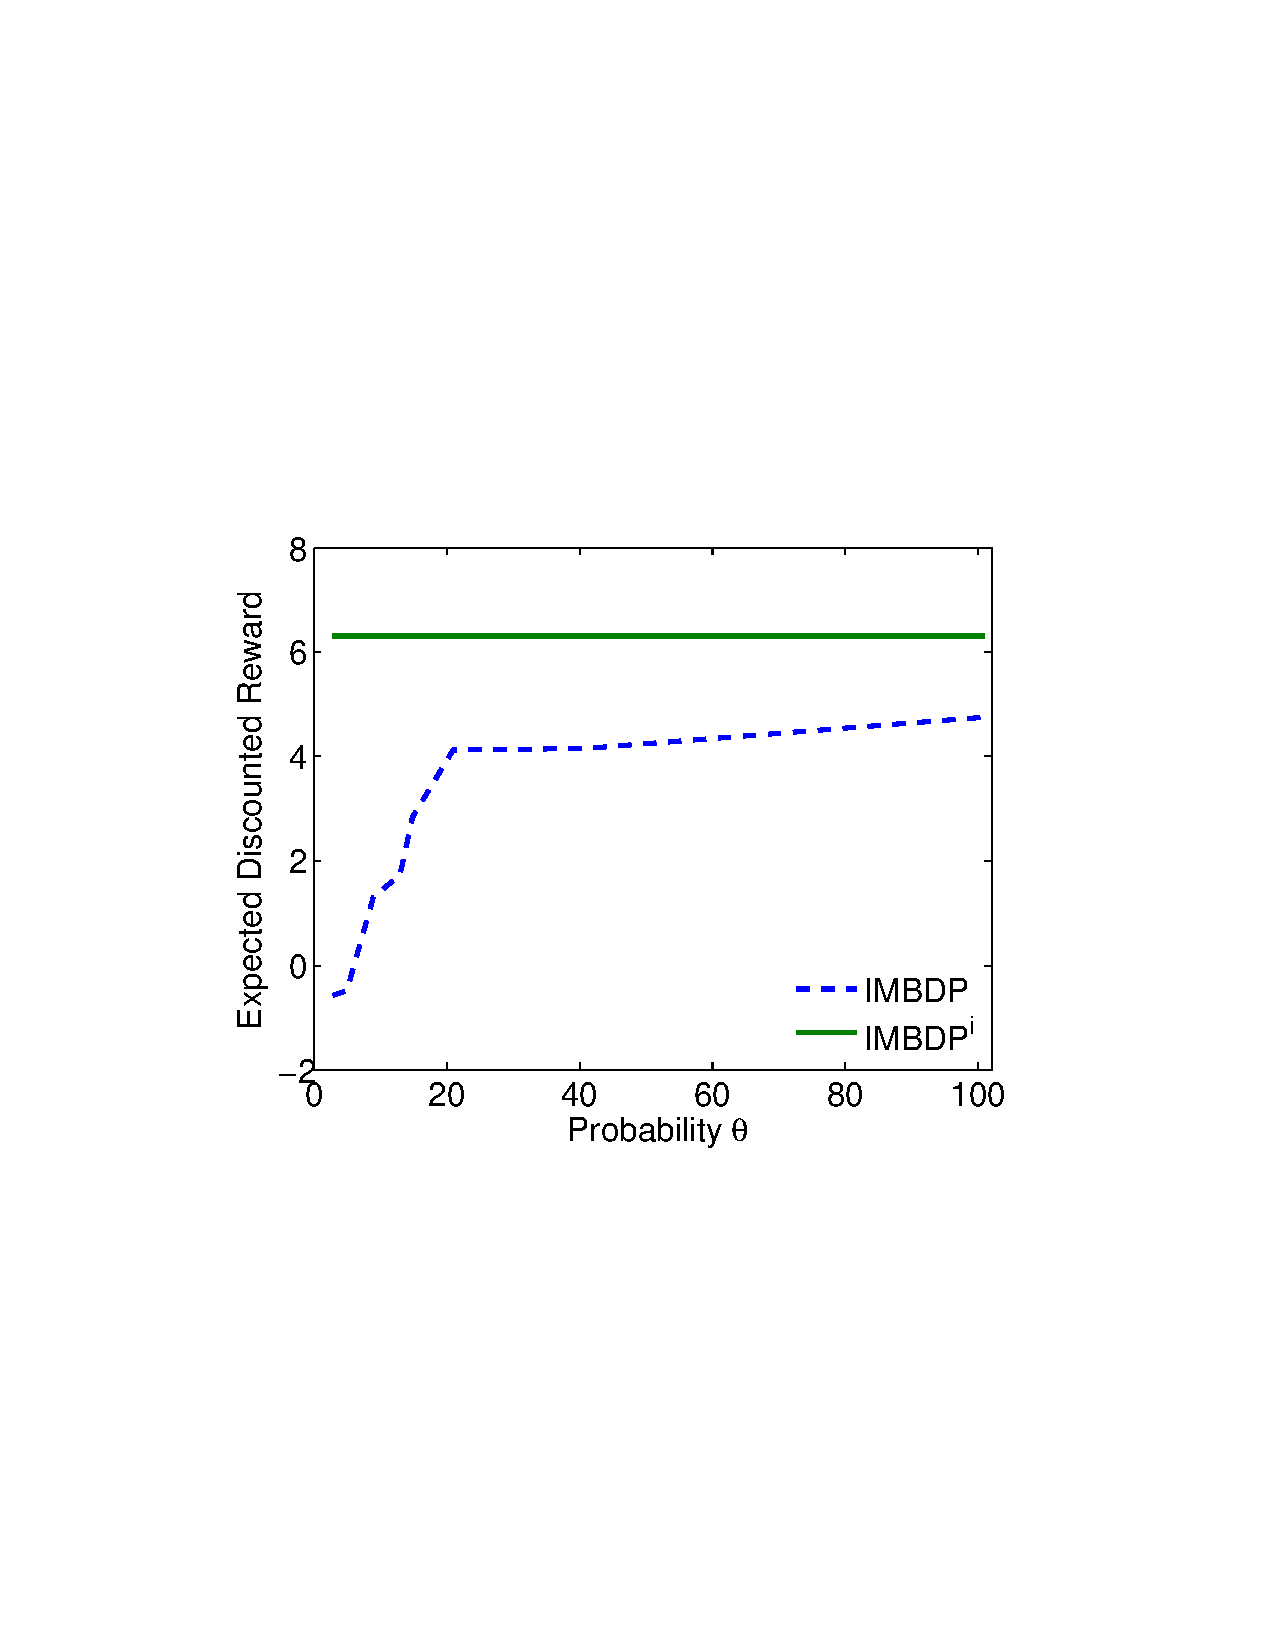
\includegraphics[width=\textwidth]{detdec22}
%  \caption{Valeur esp�r�e escompt�e � horizon fini pour diff�rentes valeurs d'horizons.}\label{fig:res_2}
%  \end{minipage}
%\end{figure*}

La figure~\ref{fig:res_3} montre le temps de calcul n�cessaire � l'approximation de la politique � horizon infini en utilisant les m�mes param�tres pour l'algorithme \textsc{imbdp}. Comme esp�r�, le temps diminue rapidement � mesure que $\theta$ cro�t puisque l'horizon n�cessaire de planification diminue �galement.

\begin{figure}[h!tb]
    \centering
    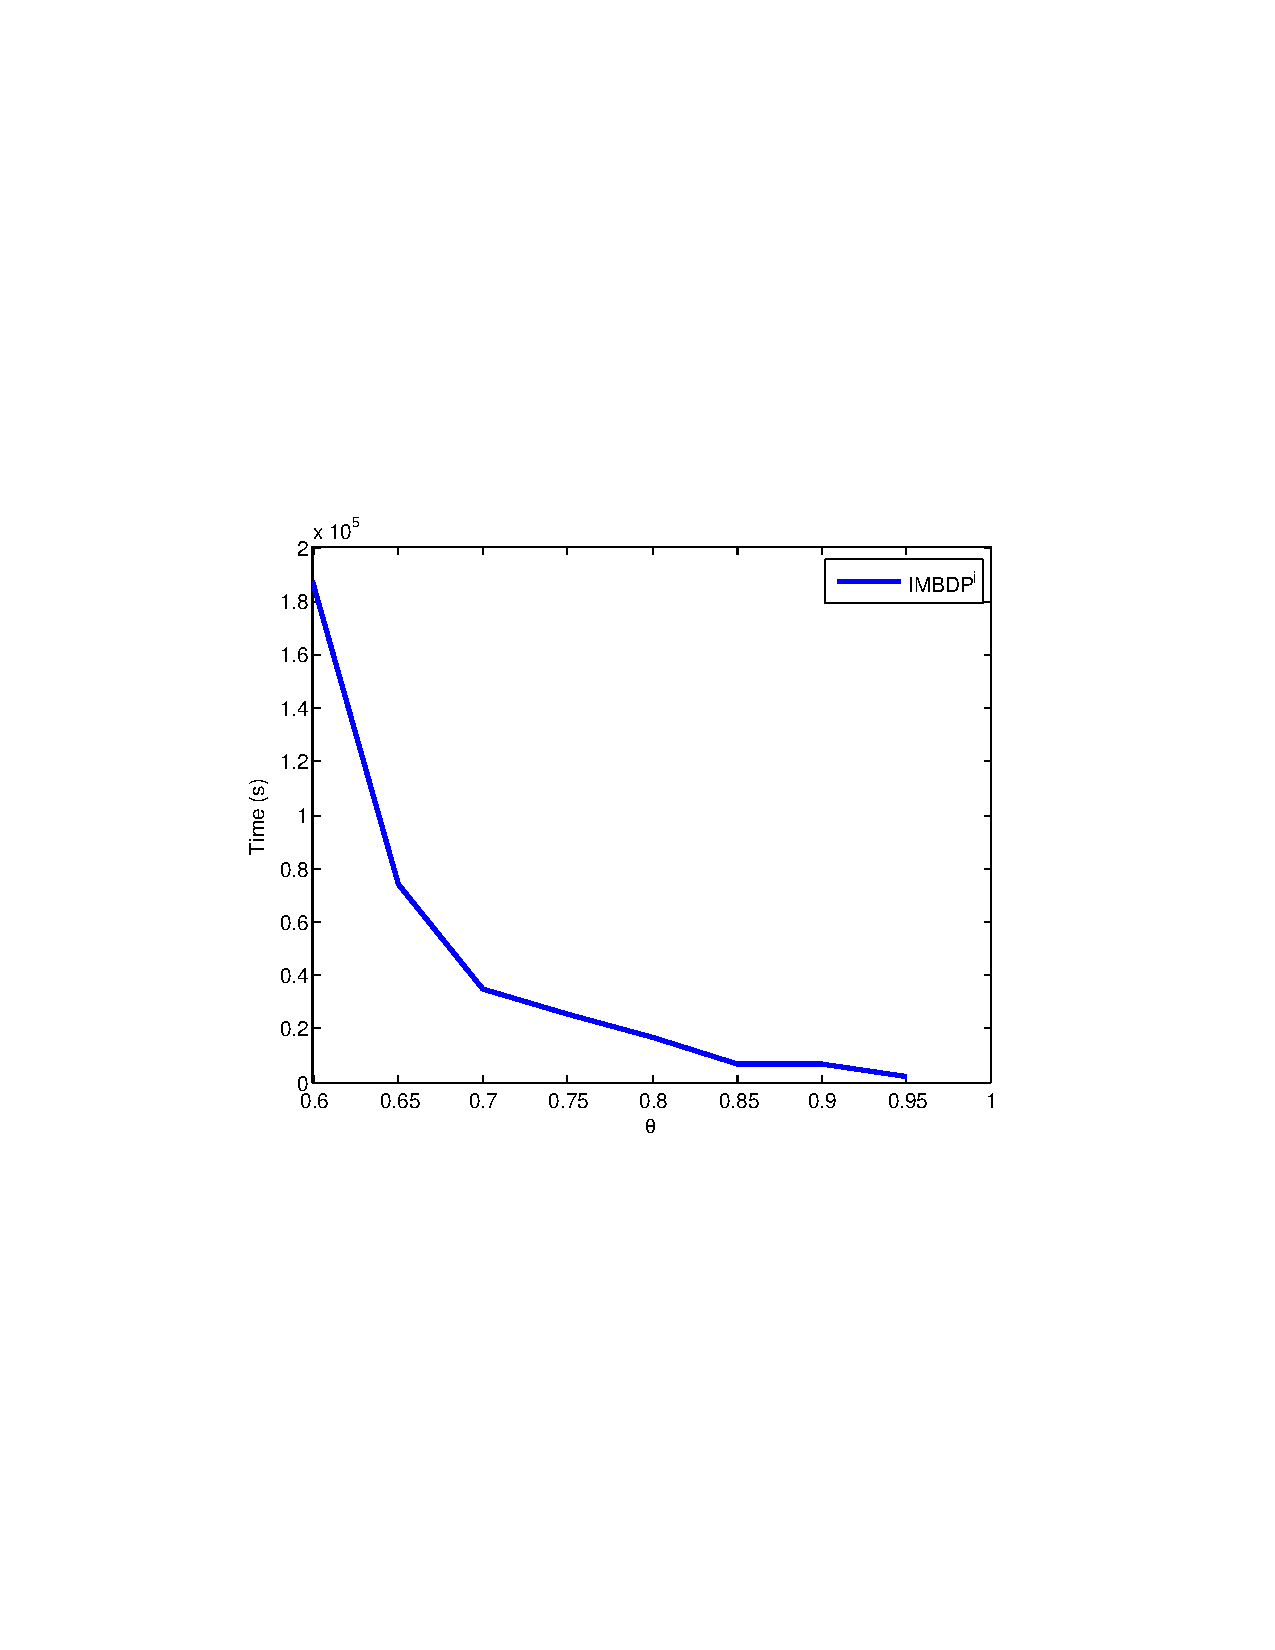
\includegraphics[width=.65\textwidth]{detdec3}
    \caption{Temps de calcul pour diff�rentes valeurs de $\theta$.}\label{fig:res_3}
\end{figure}

%\begin{figure*}[h!tb]
%\centering
%  \begin{minipage}{.48\textwidth}\centering
%    \centering
%    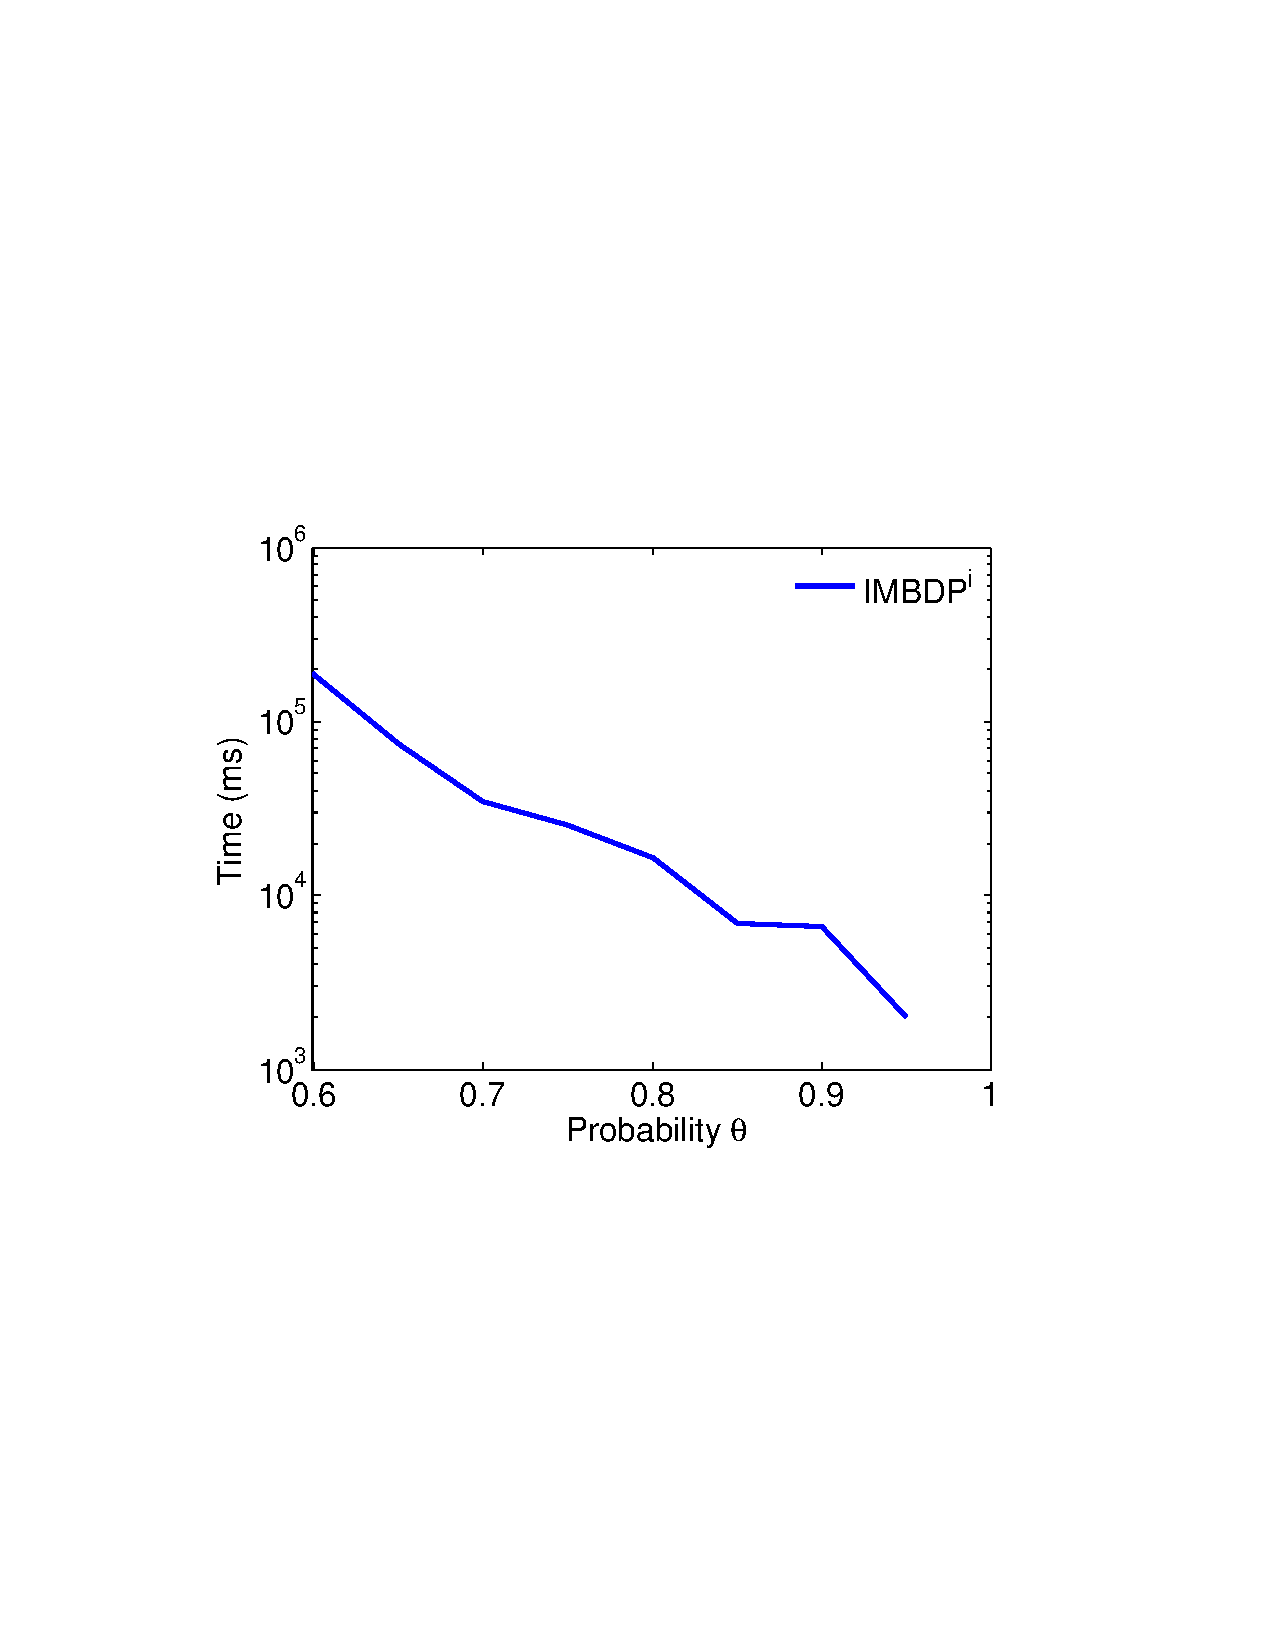
\includegraphics[width=\textwidth]{detdec32}
%    \caption{Temps de calcul pour diff�rentes valeurs de $\theta$.}\label{fig:res_3}
%  \end{minipage}
%  ~
%  \begin{minipage}{.48\textwidth}\centering
%    \centering
%    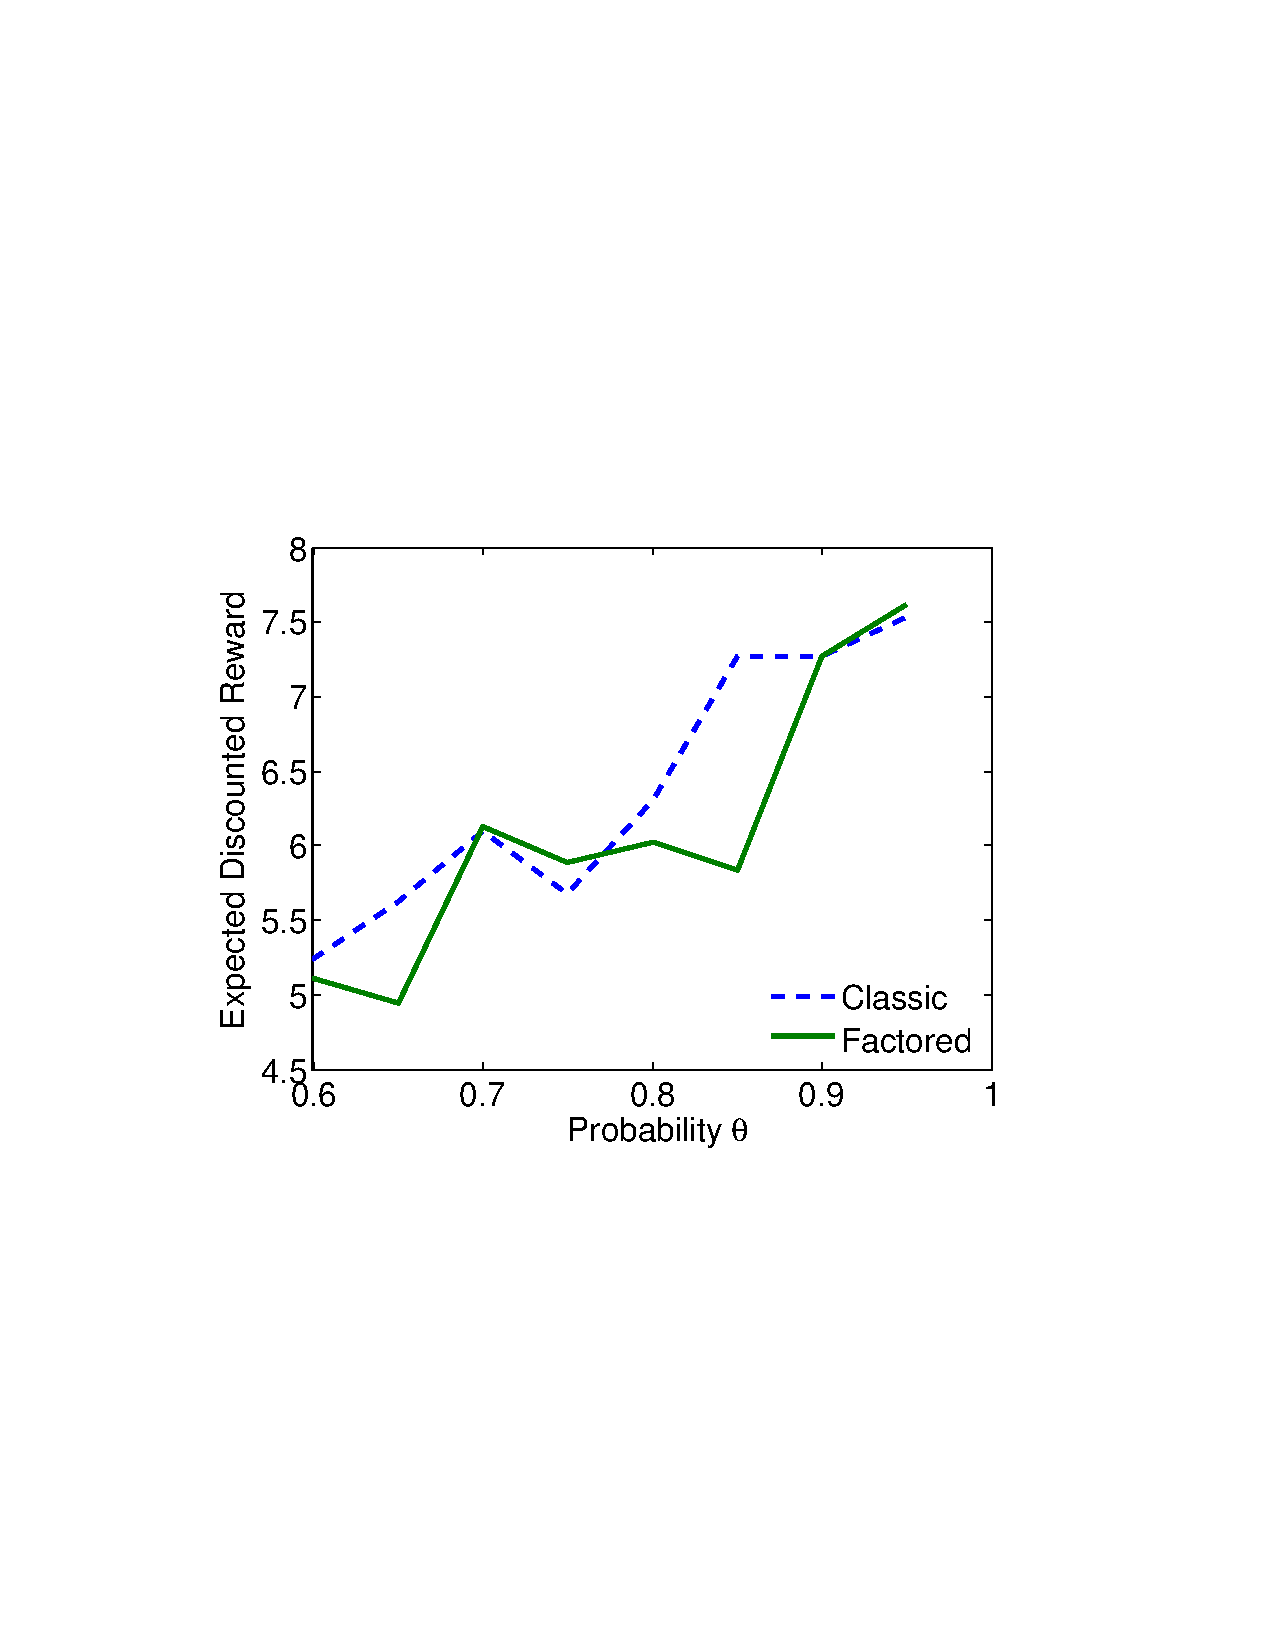
\includegraphics[width=\textwidth]{RewFire2}
%    \caption{Comparaison en valeur des mod�les classique et factoris�.}\label{fig:res_4}
%  \end{minipage}
%\end{figure*}

Les figure~\ref{fig:res_4} �~\ref{fig:res_6} comparent respectivement la valeur esp�r�e escompt�e obtenue, l'horizon n�cessaire de planification et le temps de calcul de l'algorithme \textsc{imbdp}$^i$ entre le cas d'observabilit� bijective classique et le cas factoris�. Comme l'on pouvait s'y attendre, le cas factoris� n�cessite un horizon de planification sup�rieur puisque la borne est plus l�che du fait que chaque agent re�oit moins d'information � chaque �tape. Cependant, le temps de calcul est lui bien inf�rieur (d'un ordre de grandeur) pour algorithme \textsc{imbdp}$^i$ puisque le nombre d'observations � consid�rer est beaucoup plus petit (de $49$ � $10$). Du c�t� de la valeur, les deux mod�les �tudi�s se comportent de mani�re similaire avec un l�ger avantage pour le cas classique encore d� au fait que l'information sur l'�tat est disponible plus rapidement dans ce cas-ci.


\begin{figure}[h!tb]
    \centering
    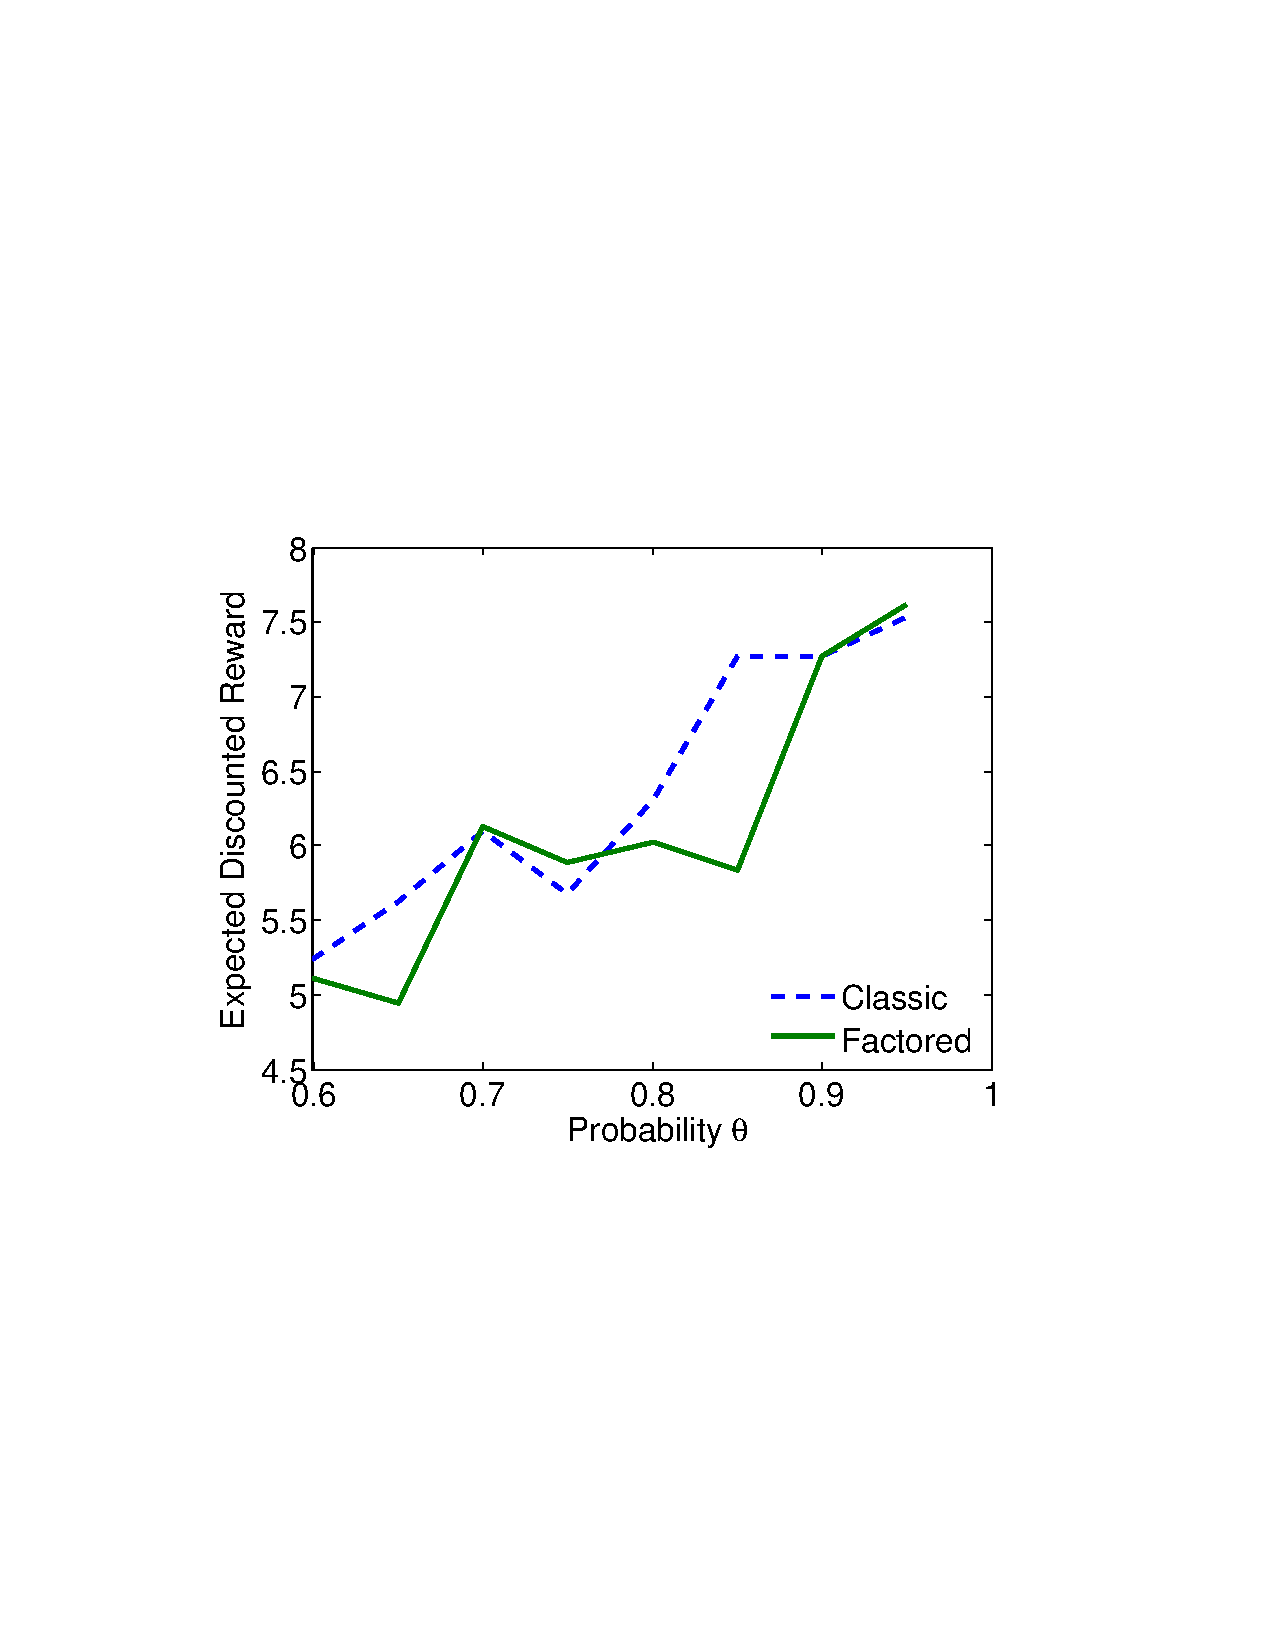
\includegraphics[width=.65\textwidth]{RewFire2}
    \caption{Comparaison en valeur des mod�les classique et factoris�.}\label{fig:res_4}
\end{figure}

\begin{figure}[h!tb]
    \centering
    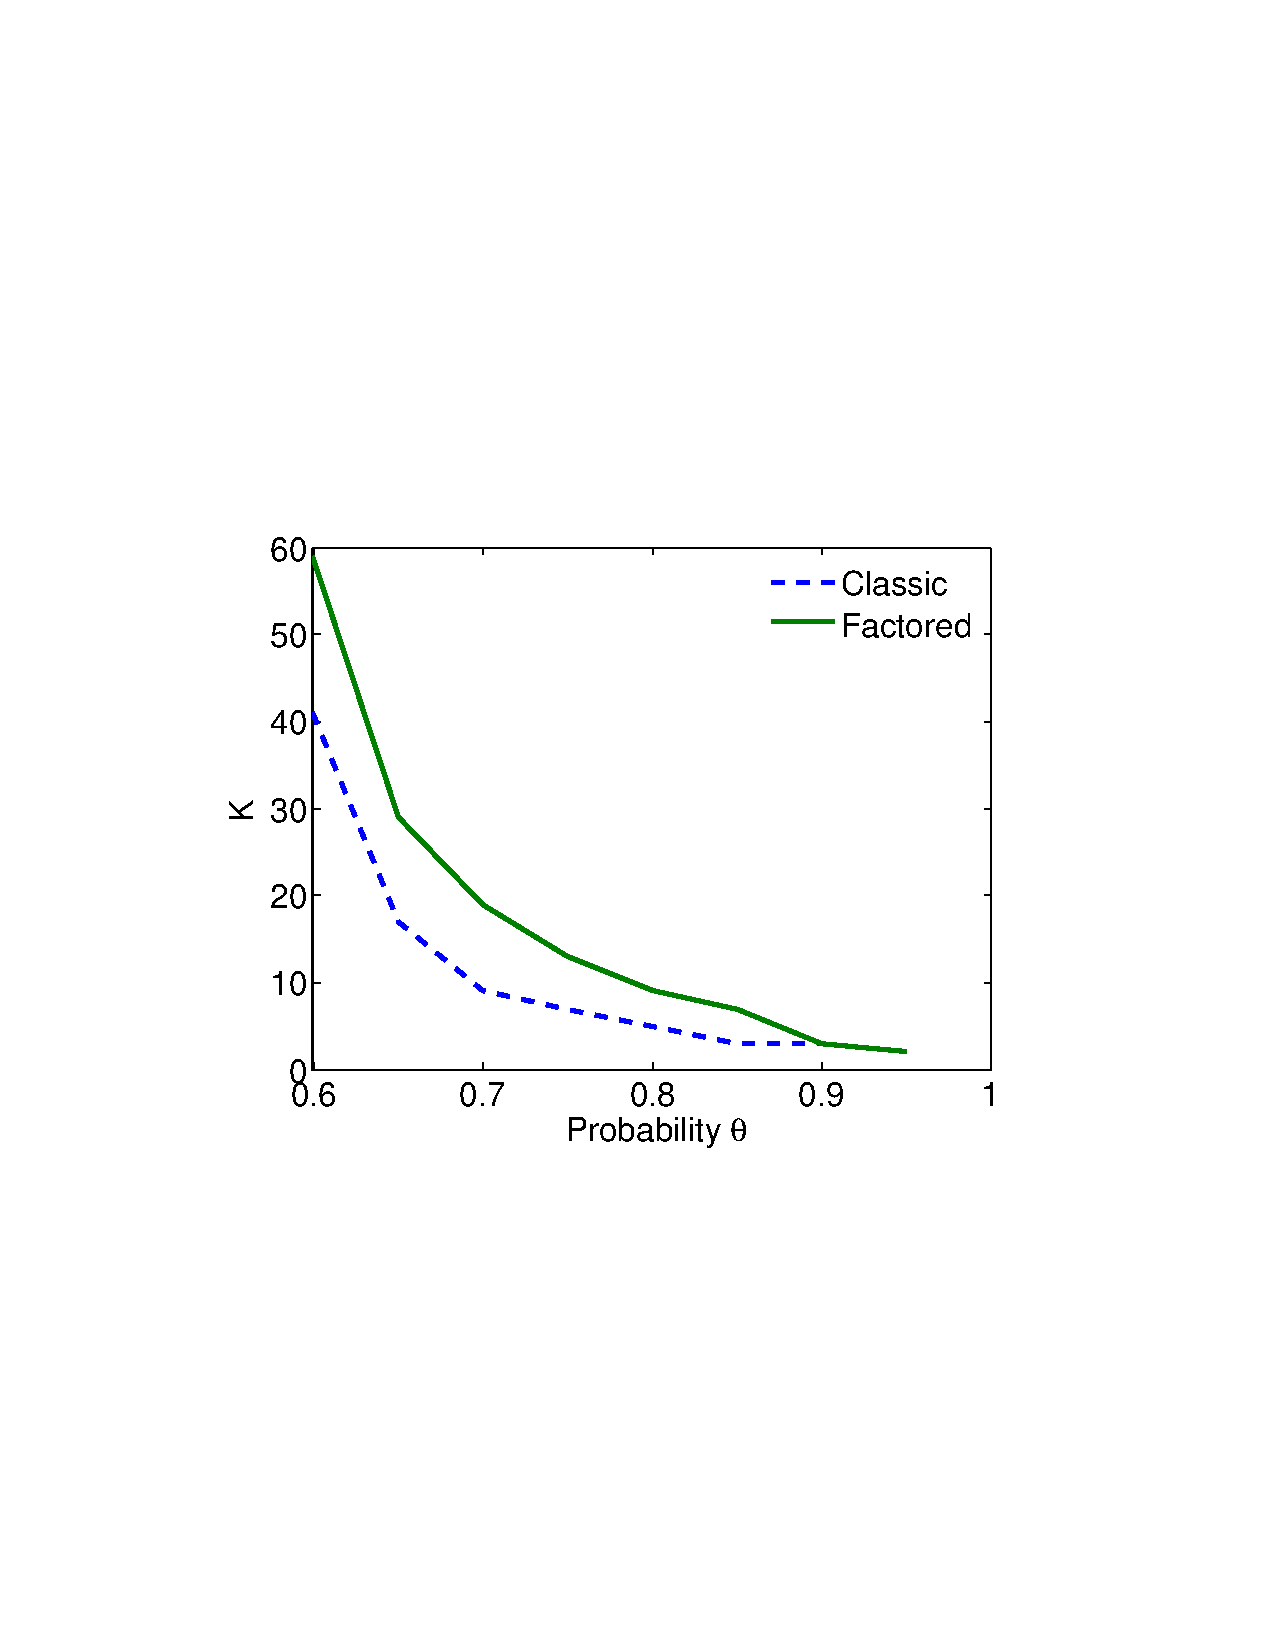
\includegraphics[width=.65\textwidth]{KFire2}
    \caption{Comparaison en horizon des mod�les classique et factoris�.}\label{fig:res_5}
\end{figure}

\begin{figure}[h!tb]
    \centering
    \includegraphics[width=.65\textwidth]{TimeFire2}
    \caption{Comparaison en temps de calcul des mod�les classique et factoris�.}\label{fig:res_6}
\end{figure}

%\begin{figure*}[h!tb]
%\centering
%  \begin{minipage}{.48\textwidth}\centering
%    \centering
%    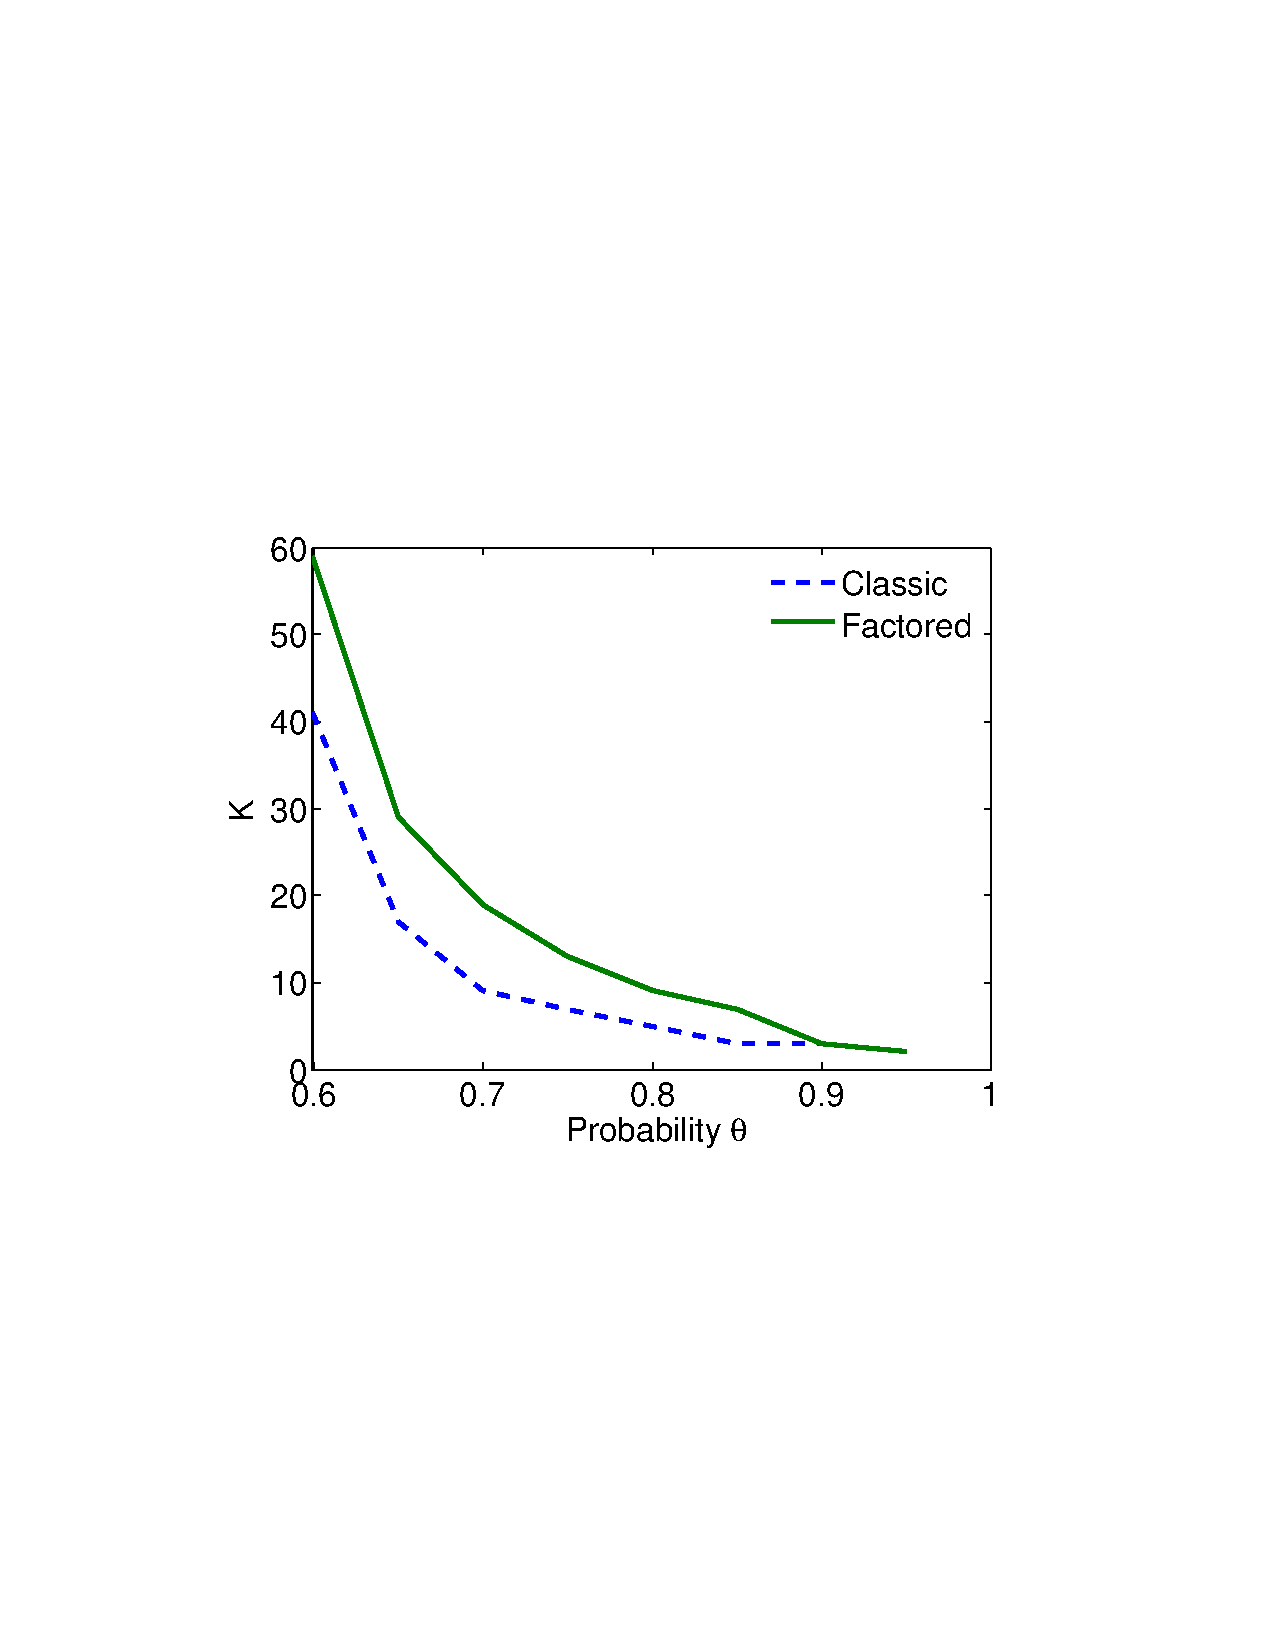
\includegraphics[width=\textwidth]{KFire2}
%    \caption{Comparaison en horizon des mod�les classique et factoris�.}\label{fig:res_5}
%  \end{minipage}
%  ~
%  \begin{minipage}{.48\textwidth}\centering
%    \centering
%    \includegraphics[width=\textwidth]{TimeFire2}
%    \caption{Comparaison en temps de calcul des mod�les classique et factoris�.}\label{fig:res_6}
%  \end{minipage}
%\end{figure*}

Discutons maintenant de l'approche g�n�rale, des hypoth�ses utilis�es, des r�sultats obtenus ainsi que des diff�rents travaux futurs avant de conclure.

\section{Discussion et Conclusion}\label{c4:s:dtc}

La premi�re chose qu'il convient de remarquer concerne les hypoth�ses faites au travers de ce chapitre. Il peut en effet para�tre curieux d'�tudier les syst�mes de Markov � transition d�terministe lorsque l'on sait qu'historiquement ces mod�les �taient introduits avant tout pour �tudier les comportements asymptotiques de syst�mes dynamiques stochastiques. Cependant, au vu des r�centes avanc�es algorithmiques pour ces mod�les il peut �tre tr�s int�ressant de s'approprier ces algorithmes dans des cas d�terministes sp�cifiques o� l'observabilit� peut faire d�faut. Il convient donc d'�quilibrer plusieurs choses:
\begin{itemize}
\item Le choix des algorithmes stochastiques pour des probl�mes partiellement observables purement d�terministes n'est pas le plus appropri� selon~\cite{B.09}. L'auteur sugg�re d'employer plut�t des algorithmes pour les arbres de recherche ET/OU~\citep{MD.09}. En revanche, dans le cas o� l'observation est stochastique mais la transition d�terministe, les r�sultats de ce chapitre montrent qu'il n'est n�cessaire de consid�rer que les $K$ derni�res observations pour ensuite pouvoir utiliser la politique du \mdp sous-jacent comme politique $\varepsilon$-optimale.
\item Le choix du mod�le d'observation, surtout dans le cas multiagent, influence l'�quilibre des performances temps/valeurs esp�r�es de l'algorithme consid�r�. Il convient donc de savoir si, dans le cas o� l'observation peut �tre factoris�e, il est pr�f�rable de ne consid�rer que certaines parties de l'observation � chaque �tape, ou s'il faut consid�rer l'observation compl�te. Dans le premier cas, l'algorithme b�n�ficie d'un avantage certain dans la complexit� en temps de calcul, mais produit des solutions � valeur moindre, alors que dans le second cas, les temps de calcul peuvent s'av�rer prohibitifs pour obtenir un gain en valeur possiblement avantageux.
\end{itemize}

La seconde chose � remarquer concerne l'hypoth�se de l'observabilit� bijective. Il est possible en effet de trouver cette hypoth�se tr�s restrictive dans certains contextes. En robotique toutefois, la factorisation du domaine et des observations est inh�rente aux capteurs attach�s au robot et cette formulation devient alors naturelle lorsque l'on observe des positions \textsc{gps} (pour \emph{Global Positioning System}) bruit�es ou des caract�ristiques sp�cifiques de l'environnement � l'aide de capteurs plus ou moins fiables. Cette �tude permet ainsi de s�lectionner dans certains cas les capteurs adapt�s au robot souhait� maximisant ainsi l'�quilibre entre la pr�cision voulue des capteurs selon la capacit� de calcul du robot, et le prix de ces capteurs, sous l'hypoth�se que des capteurs plus fiables co�tent plus cher.

Dans le cas multiagent, cette hypoth�se de bijectivit� n'est pas aussi restrictive qu'on pourrait le croire. M�me si chaque agent per�oit effectivement l'�tat \emph{complet} du monde avec une certaine probabilit�, chaque agent ne re�oit pas n�cessairement la m�me observation que les autres agents et leurs croyances sur l'�tat r�el sous-jacent du syst�me peuvent-�tre diff�rentes. D'un c�t�, cette hypoth�se semble donc plus difficilement applicable dans le cadre d�centralis� (\decpomdp) que dans le cadre centralis� (\pomdp) puisque les valeurs de variables internes aux agents ne sont alors plus obligatoirement observables. D'un autre c�t�, ces variables internes peuvent �ventuellement �tre transmises � autrui sans n�cessairement communiquer leur observation compl�te, et l'incertitude sur cette communication peut �tre alors incluse dans l'incertitude associ�e � l'observabilit� de ces variables.

Dans la litt�rature, cette hypoth�se d'observabilit� bijective s'approche beaucoup des travaux effectu�s par~\cite{GZ.04} sur les \decmdps o� les agents, lorsqu'ils communiquent leurs observations, ont acc�s � l'�tat r�el sous-jacent du syst�me. La diff�rence avec ces travaux provient du fait que chacun des agents ne per�oit pas sa propre partie de l'�tat avec certitude, fournissant ainsi � l'ensemble du syst�me l'observabilit� compl�te au travers de la communication. L'observabilit� bijective assure uniquement que chaque agent \emph{peut �ventuellement} observer l'�tat r�el du syst�me avec probabilit� $\theta$. En d'autres termes, un \decmdp avec communication compl�te est un \decpomdp avec observabilit� bijective o� $\theta = 1$, qui est aussi un \mmdp.

En termes de travaux futurs, deux voies restent � �tre explor�es. Une premi�re concerne l'extension de ce mod�le aux probl�mes avec transition quasi-d�terministe et le contr�le dans ce domaine. Des travaux non publi�s pr�sent�s dans la section~\ref{anx:it} utilisant des notions de th�orie de l'information montrent qu'il est impossible de montrer la convergence de l'�tat de croyance vers une entropie nulle comme l'on laiss� entendre les figures~\ref{fig:entropy:3} �~\ref{fig:entropy:97}. Il est toutefois envisageable, comme le montre les travaux de~\cite{HLR.07} sur l'approximabilit� des \pomdps, de trouver des classes de fonctions de transitions particuli�res for�ant la convergence des �tats de croyance vers un ensemble fini d'�tats de croyance sur lesquels des algorithmes d'it�ration de valeur seraient applicables par exemple. La seconde avenue consiste � consid�rer un probl�me r�el permettant de mettre en \oe uvre ce mod�le et des travaux ont �t� commenc�s en ce sens avec Jean-Samuel Marier sur un syst�me de patrouille d'\textsc{uav}s (pour \emph{Unmanned Aerial Vehicles})~\citep{MBC.09,MBC.10} ou plusieurs agents doivent surveiller un ensemble de positions strat�giques r�guli�rement et s'adapter en cas de changement des positions ou en cas de dysfonctionnement des \textsc{uav}s.

Dans le chapitre suivant nous allons donc nous concentrer sur les aspects distribu�s de la planification en ligne et particuli�rement sur l'�tat de croyance lorsque les agents ne communiquent pas n�cessairement. 
\newpage\phantom{a}

% DecPOMDPs et Communication
\chapter{Observabilit� et communication dans les processus de Markov d�centralis�s}

% \emph{�Ce qui est important c'est l'esprit d'�quipe. Les mecs, y sont une �quipe, y'a un esprit, alors forcement, il faut qu'ils partagent.�}
% \begin{flushright} Coluche \end{flushright}
% \bigskip

\emph{�Coop�rer, c'est r�soudre � deux des probl�mes qu'on n'aurait jamais eus tout seul.�}
\begin{flushright} adapt� de Sacha Guitry \end{flushright}
\bigskip

\label{chap:5}

\begin{summary}
Ce chapitre introduit tout d'abord la r�solution en ligne de processus d�cisionnels de Markov d�centralis�s (\decpomdps) puis pr�sente un algorithme approximatif et � utilisation de m�moire constante dans le cas o� aucune communication n'est autoris�e. L'algorithme est ensuite �valu� empiriquement sur diff�rents probl�mes de la litt�rature et ses r�sultats sont compar�s � des adaptations en ligne des meilleurs algorithmes disponibles. Une discussion de ces r�sultats est �galement effectu�e ainsi que les diff�rentes extensions possibles autour de la communication.
\end{summary}

\section{Introduction � la r�solution en ligne de \pac{dec-pomdp}s}

Comme l'a soulign� le chapitre pr�c�dent, l'observabilit� est un facteur cl� de la complexit� d'un probl�me de planification multiagent. D�s lors que l'observabilit� n'est plus bijective en regard de l'�tat, le probl�me devient alors extr�mement complexe (\textsc{nexp}-complet) et l'on doit alors faire appel � des algorithmes d'approximation d�pourvus de garanties, l'approximabilit� de ce type de probl�me ayant �t� montr�e au moins tout aussi complexe (\textsc{nexp}-difficile)~\citep{RGR.03}.

Parmi ces algorithmes d'approximation, plusieurs ont �t� pr�sent�s au chapitre~\ref{chap:2} de cette th�se, et ils s'av�rent �tre tous une r�solution \emph{hors ligne} du probl�me de planification markovienne multiagent d�centralis�. Le \emph{hors ligne} signifie pr�cis�ment que toute la planification est r�alis�e \emph{avant} l'ex�cution et qu'aucune planification n'est effectu�e une fois que l'ex�cution a commenc�. Par opposition, \emph{en ligne} signifie que l'agent peut planifier entre deux ex�cutions d'actions dans l'environnement et peut donc utiliser l'information r�colt�e pendant l'ex�cution pour am�liorer sa planification. Les avantages de la planification en ligne sont doubles: il n'est pas n�cessaire de planifier pour l'ensemble des �tats de croyance possible (soit le simplexe au complet), et l'int�gration de la connaissance acquise au cours du temps se fait naturellement � chaque re-planification � partir de l'�tat de croyance courant. Tr�s r�pandus dans le contexte monoagent \pomdp (avec \textsc{rtbss}~\citep{PTC.06}, \textsc{aems}~\citep{RC.07,RPCP.08}), le probl�me de la planification en ligne en multiagent et dans le cas partiellement observable provient de la connaissance d�centralis�e de l'�tat et du fait que les agents ne partagent justement pas la m�me croyance sur l'�tat courant selon leurs observations respectives.

Ce chapitre pr�sente donc un algorithme d�centralis� de planification en ligne pour les \decpomdps. Dans un premier temps, l'algorithme dont s'inspire notre propre algorithme sera pr�sent�. Il s'agit de l'algorithme de \emph{Rollout} de~\cite{BTW.97} qui a �t� pens� et r�alis� pour le cas monoagent compl�tement observable (\mdp). L'extension au cas multiagent partiellement observable sera ensuite pr�sent�e et �valu�e empiriquement avant de conclure. L'algorithme de \emph{Rollout} est maintenant d�taill�.

\section{Algorithme � base de ``rollouts''}

Le principe de base de l'algorithme de Rollout, tel que pr�sent� par \cite{BTW.97}, consiste � faire de l'am�lioration incr�mentale en ligne de politique. Cette m�thode n�cessite une politique $\pi$ qu'on am�liore ensuite successivement � l'aide de trajectoire Monte-Carlo par exemple. Pour cela, � chaque �tape de temps, le Rollout consid�re l'�tat courant et calcule l'ensemble des �tats suivants possibles � partir des actions disponibles. Puis, il approxime la valeur esp�r�e de la politique $\pi$ dans chaque �tat suivant g�n�r� � l'aide de simulations Monte-Carlo, et cette �valuation est ensuite utilis�e pour s�lectionner la meilleure action disponible qui peut �ventuellement �tre diff�rente de celle sugg�r�e initialement par la politique $\pi$. L'action s�lectionn�e se trouve ainsi �tre celle ayant la plus grande valeur esp�r�e (toujours selon l'estimation Monte-Carlo) dans l'�tat courant. Il est en fait possible de montrer, dans le cas monoagent et sous certaines conditions l�g�res, que la politique effectivement ex�cut�e produit une valeur esp�r�e au moins aussi �lev�e que la politique $\pi$ initiale, � moins que la politique $\pi$ soit optimale, auquel cas, le Rollout se comporte alors aussi optimalement.

Dans ce contexte, \cite{CGC.04} ont propos� une extension de cet algorithme au cas monoagent partiellement observable (\pomdp) en utilisant les �tats de croyance plut�t que les �tats directement. Ainsi, dans le cas des \pomdps, le Rollout calcule, � partir de l'�tat de croyance courant de l'agent, l'ensemble des �tats de croyance possibles selon les actions disponibles et les observations r�sultantes possibles. Une estimation de la valeur de ces �tats de croyance est �galement �valu�e � partir de simulation Monte-Carlo non plus d'une seule politique initiale $\pi$ mais d'un ensemble de politiques de base $\Pi$. La meilleure action -- correspondant � la meilleure valeur esp�r�e -- est ensuite retourn�e. L'algorithme~\ref{alg:rollout} donne le pseudo-code du cas partiellement observable.

\begin{algorithm}[htb]\caption{Rollout pour \pomdp \label{alg:rollout}}
\algrenewcommand\alglinenumber{\tiny}
   \begin{algorithmic}[1]
   \Require{Un ensemble d'heuristiques $\Pi = \la \pi_1,\ldots,\pi_m\ra$, un �tat de croyance $\bel^0$ et un horizon $T$.}
   \Ensure{Une action que l'agent doit ex�cuter dans l'�tat de croyance $\bel^0$.}
    \vspace{5pt}
    \Function{Rollout}{$\Pi$,$\bel^0$,$T$}
        \ForAll{$a\in\Act$, $o\in\Obs$}
            \State{$\{\bel^1\}_{a,o} \gets$ \textsc{Update}($\bel^0,a,o$)}\Comment{Mise � jour de l'�tat de croyance (Eq. \ref{BeliefUpd})}
            \ForAll{$\bel^1 \in \{\bel^1\}_{a,o}$}
                \State{$\Upsilon \gets$ \textsc{smce}($\Pi, \bel^1, T$)\label{alg:roll:smce}}\Comment{Valeur estim�e des simulations Monte-Carlo}
            \EndFor
        \EndFor
        \State{$a^\star \gets \arg\max\limits_{a\in\Act} \sum\limits_{o \in \Obs} \Pr(o|\bel^0, a) \max\limits_{\pi \in \Pi} \Upsilon[\pi]$}
    \State{\Return{$a^\star$}}
    \EndFunction
   \end{algorithmic}
\end{algorithm}
L'estimation de la valeur des politiques par simulation Monte-Carlo (� la ligne~\ref{alg:roll:smce} de l'algorithme~\ref{alg:rollout}) not�e \textsc{smce}$(\Pi, \bel^1, T)$ sera plus amplement expliqu�e � la section~\ref{sect:smce}. Voyons maintenant l'extension au cas multiagent.

\section{Rollout d�centralis� (dRollout)}

L'approche propos�e dans ce chapitre est similaire � celle de \cite{BTW.97} et de \cite{CGC.04} dans l'utilisation et l'am�lioration d'heuristiques. Une estim�e de la valeur esp�r�e de chaque politique donn�e est calcul�e pour chaque action que peut r�aliser un agent en se basant sur des m�thodes Monte-Carlo s�quentielles. L'approche utilise ainsi une quantit� fixe de temps et de m�moire � chaque it�ration d'am�lioration. Plus formellement, �tant donn� un ensemble d'heuristiques multiagent $\Pi$ selon un �tat de croyance multiagent, la politique associ�e au Rollout s�lectionne l'action selon l'�quation suivante:
\[\ba = \arg\max_{\ba\in\JAct} \max_{\pi \in \Pi} \Esp\left[\sum_{t=0}^T \Rew(\bel^t, \pi(\bel^t))\right]\]
O� $\Rew(\bel^t,\ba)$ est la r�compense esp�r�e selon l'�tat de croyance $\bel^t$:
\[\Rew(\bel^t,\ba) = \Esp_{s\in\Sta}\left[ \Rew(s,\ba) \right] = \sum_{s\in\Sta} \bel^t(s) \Rew(s,\ba)\]

Un des probl�mes de l'algorithme de Rollout provient de sa n�cessit� d'avoir des \emph{bornes inf�rieures} sur la fonction de valeur optimale pour garantir que le choix de l'action sera bien meilleur. De fait, toute politique sous-optimale permettra de diriger la recherche de l'algorithme Rollout de mani�re correcte. C'est pour cela, qu'en sus des bornes disponibles dans la litt�rature, rappel�es � la section~\ref{sect:dp} du chapitre~\ref{chap:2}, nous avons choisi aussi d'utiliser l'algorithme \mbdp et ses d�riv�s de la section~\ref{sect:mbdp} du chapitre~\ref{chap:2} et une version en ligne de la programmation dynamique (section~\ref{sect:dp} du chapitre~\ref{chap:2}) -- qui utilise un horizon ``mobile'' de 2 pour s�lectionner la meilleure action --  comme borne inf�rieure sur la valeur optimale. Voyons maintenant comment �valuer ces heuristiques � l'Aide de simulation Mont-Carlo.

\subsection{Simulations Monte-Carlo}\label{sect:smce}

Les simulations Monte-Carlo (cf. annexe~\ref{anx:pf}), bien qu'efficaces, sont surtout reconnues pour consommer beaucoup de temps de calcul. Cependant, de r�cents travaux ont consid�rablement r�duit les temps de simulation. Ces techniques, appel�es \emph{filtres � particules}, permettent la simulation en parall�le de plusieurs essais Monte-Carlo s�quentiels tout en utilisant une taille fixe de la m�moire et offrant des garanties de performance sur l'estimation de la distribution de probabilit� post�rieure.

\cite{T.99} a appliqu� la technique des filtres � particules avec succ�s aux \pomdps. Il estimait l'�tat de croyance � chaque �tape de temps � l'aide de filtres � particules puis s�lectionnait ensuite la meilleure action � ex�cuter en utilisant une proc�dure mixant programmation dynamique et l'algorithme des \emph{k-plus-proches-voisins} pour la g�n�ralisation. Les filtres � particules �taient utilis�s comme variante � base d'�chantillons des filtres de Bayes pour r�cursivement estimer la densit� post�rieure, ou l'�tat de croyance $\bel$, sur un �tat $s$, du syst�me dynamique~\citep{FTBD.01}:
\[\bel^{t+1}(s') \propto \Obs(\bo|\ba,s') \int \Tra(s'|s,\ba) \bel^t(s)\,\mathrm{d}s\]
O�, comme d�fini pr�c�demment, $\bo$ est l'observation jointe re�ue et $\ba$ l'action jointe effectu�e.

Le filtre � particules repr�sente l'�tat de croyance par un ensemble $S$ de $N$ particules pond�r�es $\la s^{(i)}, w^{(i)}\ra$. Chaque $s_{(i)}$ est un �chantillon repr�sentant un �tat, et les $w^{(i)}$ sont des r�els non n�gatifs, appel�s \emph{poids d'importance}, qui somment � un. Dans sa forme basique, le filtre � particule r�alise un filtrage bay�sien r�cursif selon une proc�dure d'�chantillonnage souvent r�f�r�e par l'\emph{�chantillonnage s�quentiel par importance avec r��chantillonnage} (\textsc{sisr}):
\begin{enumerate}
\item[1.] \emph{�chantillonnage}: Utilise l'�tat courant $s$ et l'action jointe\footnote{Il est �galement possible d'utiliser une distribution sur les actions plut�t que l'action seule.} $\ba$ pour �chantillonner l'�tat suivant $s'$ selon la fonction de transition $\Tra(s'|s,\ba)$, qui d�crit la dynamique du syst�me selon l'interaction de l'agent;
\item[2.] \emph{Pond�ration des �chantillons}: Pond�re l'�chantillon $s'$ par la vraisemblance de l'observation $w' = \Obs(\bo|s,\ba,s')$. Cette vraisemblance est extraite de la fonction d'observation de l'agent (e.g. du mod�le de ses capteurs et de l'environnement) .
\item[3.] \emph{R��chantillonnage}: Tire avec remplacement un nouvel �chantillon -- un �tat -- $s$ de l'ensemble $S$ (repr�sentant l'�tat de croyance courant $\bel(s)$) selon la distribution discr�te d�finie par la pond�ration $w^{(i)}$ appliqu�e � l'�tape pr�c�dente.
\end{enumerate}

Dans certains cas, toutefois, les filtres � particules peuvent prendre du temps � faire cette mise � jour de l'�tat de croyance, quand le nombre de particules est beaucoup trop grand par exemple. Dans ces cas ci, des am�liorations existent dans la litt�rature. Parmi ceux-ci, un des plus int�ressants est le filtre adaptatif et temps-r�el de~\cite{KFM.03}. Il permet de d�terminer dynamiquement le nombre de particules � utiliser � chaque instant pour garantir une borne sur l'erreur faite sur l'approximation de l'�tat de croyance selon la divergence de Kullback-Leibler (\textsc{kl} divergence).

Si l'on suppose que la distribution discr�te estim�e est r�partie dans $k$ ``bo�tes'' (e.g. l'�tat de croyance est r�parti sur $k$ �tats), alors, pour des bornes sur l'erreur fixes $\varepsilon$ et $\delta$, l'�quation~\eqref{eq:pfkld} donne le nombre d'�chantillons $N$ minimal en fonction de $k$~\citep{F.01} tel que, avec probabilit� $1-\delta$, la \textsc{kl} divergence entre l'estim�e du maximum de vraisemblance bas�e sur les �chantillons et la vraie distribution \emph{a posteriori} n'exc�de pas un certain seuil $\varepsilon$:
\begin{equation}
N = \frac{k-1}{2\varepsilon}\left[ 1 - \frac{2}{9(k-1)} + \sqrt{\frac{2}{9(k-1)}} z_{1-\delta} \right]^3 \label{eq:pfkld}
\end{equation}

O� $z_{1-\delta}$ est le $1-\delta$-quantile sup�rieur d'une distribution normale $\mathcal{N}(0,1)$. Le nombre requis de particules est donc proportionnel � l'inverse de l'erreur voulue et lin�aire en fonction du nombre $k$ de ``bo�tes'' sur lesquelles est la distribution. L'�chantillonnage \textsc{kld} estime $k$ par le nombre d'�tats qui sont repr�sent�s par au moins une particule.

Pour int�grer l'�chantillonnage \textsc{kld} dans un algorithme de filtre � particule standard, une grille fixe est initialement utilis�e pour approximer la distribution sur les �tats (e.g. les �tats eux-m�mes). Puis, pendant la phase de pr�diction du filtrage (l'�tape 1 dans la proc�dure \textsc{sisr}), l'algorithme d�termine si un des �tats suivants g�n�r�s tombe dans une case vide de la grille ou non (la grille est remise � z�ro apr�s chaque mise � jour). Si la case de la grille est vide, alors le nombre de ``bo�tes'' $k$ est incr�ment� et la case est marqu�e comme non vide. Apr�s chaque �chantillonnage, le nombre requis d'�chantillons est mis � jour en utilisant l'�quation~\eqref{eq:pfkld}. L'�chantillonnage s'arr�te d�s lors qu'aucune nouvelle ``bo�te'' ne se remplit et que $N$ converge.

Ainsi, l'�chantillonnage \textsc{kld} utilise initialement un grand nombre de particules lorsque rien n'est connu sur l'�tat courant et donc que la distribution est uniforme. Ce m�me nombre de particules diminue ensuite rapidement � mesure que de l'information sur l'�tat arrive. Pour plus de d�tails sur les filtres temps-r�els adaptatifs, le lecteur int�ress� est invit� � se r�f�rer aux travaux de~\cite{F.01} sur le sujet. Voyons maintenant comment nous avons utilis� ces filtres dans le contexte d'un Rollout multiagent.

\subsection{Rollout d�centralis�}

Les entr�es de l'algorithme d�centralis� de Rollout sont les suivantes: un �tat de croyance joint initial $\bel^0$ qui est l'information commune partag�e par tous les agents, et un ensemble d'heuristiques (ou de politiques sous-optimales) $\Pi = \la \pi_1, \ldots, \pi_m\ra$. On suppose que cet ensemble d'heuristiques est ordonn� initialement par la valeur esp�r�e de chaque heuristique dans l'�tat de croyance initial: $EU(\pi_1,\bel^0)\ge ... \ge EU(\pi_m,\bel^0)$.

\begin{algorithm}[htb]\caption{Rollout pour \decpomdps \label{alg:drollout}}
\algrenewcommand\alglinenumber{\tiny}
   \begin{algorithmic}[1]
   \Require{Un ensemble d'heuristiques $\Pi = \la \pi_1,\ldots,\pi_m\ra$, l'�tat de croyance de l'agent $i$: $\bel_i^0$, un horizon $T$.}
   \Ensure{Une action que l'agent $i$ doit ex�cuter dans l'�tat de croyance $\bel_i^0$.}
    \vspace{5pt}
    \Function{dRollout}{$\Pi$,$\bel_i^0$,$T$}
     \State{$\ba_{-i} \gets \pi_1(\bel_i^0)$}
        \ForAll{$a\in\Act$, $\bo\in\JObs$}
            \State{$\ba \gets \la a,\ba_{-i} \ra$\label{alg:drollout:assumption1}}
            \State{$\{\bel_i^1\}_{\ba_{-i},\bo} \gets$ \textsc{Update}($\bel^0,\ba,\bo$)}
            \ForAll{$\bel_i^1 \in \{\bel_i^1\}_{\ba_{-i},\bo}$}
                \State{$\Upsilon \gets$ \textsc{smce}($\Pi, \bel_i^1, T$)}
            \EndFor
        \EndFor
        \State{$a_i^\star \gets \arg\max\limits_{a\in\Act} \sum\limits_{\bo \in \JObs} \Pr(\bo|\bel_i^0,\la a,\ba_{-i}\ra) \max\limits_{\pi \in \Pi} \Upsilon[\pi]$\label{alg:drollout:depth1}}
    \State{\Return{$a_i^\star$}\label{alg:drollout:retroll}}
    \EndFunction
   \end{algorithmic}
\end{algorithm}

L'algorithme~\ref{alg:drollout} d�crit le pseudo-code de l'algorithme de Rollout d�centralis�. L'algorithme est construit de telle sorte que chaque agent calcule tout d'abord l'�tat de croyance joint en faisant l'hypoth�se que les autres agents suivent l'heuristique la plus prolifique, i.e. la politique $\pi_1$ (ligne \ref{alg:drollout:assumption1}). L'ensemble des �tats de croyance possible $\{\bel_i^1\}_{\ba_{-i},\bo}$ est ainsi calcul� sur la base que tous les autres agents vont suivre l'heuristique $\pi_1$ et vont recevoir une observation jointe d�pendante de l'�tat de croyance courant $\bel^0$. L'ensemble des heuristiques $\Pi = \la \pi_1, \ldots, \pi_m\ra$ est alors �valu� sur chacun de ces �tats de croyance $\{\bel_i^1\}_{\ba_{-i},\bo}$ � partir des m�thodes Monte-Carlo s�quentielles pr�sent�es � la sous-section pr�c�dente et dont le pseudo-code est donn� par l'algorithme~\ref{alg:smce}.

\begin{algorithm}[htb]\caption{Estimation Monte-Carlo s�quentielle de chaque $\pi \in \Pi$ \label{alg:smce}}
\algrenewcommand\alglinenumber{\tiny}
   \begin{algorithmic}[1]
   \Require{Un ensemble d'heuristiques $\Pi = \la \pi_1,\ldots,\pi_m\ra$, un �tat de croyance $\bel_i^1$, un horizon $T$.}
   \Ensure{Une valeur esp�r�e pour chaque heuristique fournie pour l'�tat de croyance consid�r� $\Upsilon = \la EU(\pi_1,\bel_i^1),\ldots,EU(\pi_m,\bel_i^1)\ra$.}
\vspace{5pt}
    \Function{smce}{$\Pi$,$\bel_i^1$,$T$} \label{alg:smce:mce}
    \ForAll{$\pi_k\in\Pi$}
        \For{$t=1$ \textbf{jusqu'�} $T-1$}
            \State{$\phi_{-i}^{\pi_k} \sim \la \pi_k, \mathcal{U}(\{\pi_j(\bel_i^1)\})\ra$\label{alg:smce:anyPol}}\hfill\Comment{D�finit l'heuristique jointe stochastique}
            \State{$\bel_i^{t+1} \gets$ \textsc{Step}($\bel_i^t,\phi_{-i}^{\pi_k}$)\label{alg:smce:update}}\hfill\Comment{Calcule l'�tat de croyance suivant par \textsc{sisr}}
        \EndFor
        \State{$V_{\pi_k}(\bel_i^{T}) \gets \Rew(\bel_i^{T}, \phi_{-i}^{\pi_k}(\bel_i^T))$}\hfill\Comment{�value $\pi_k(\bel_i^{1})$}
        \For{$t=T-1$ \textbf{jusqu'�} $1$}
            \State{$V_{\pi_k}(\bel_i^{t}) \gets \Rew(\bel_i^{t}, \phi_{-i}^{\pi_k}(\bel_i^t)) + V_{\pi_k}(\bel_i^{t+1})$}
        \EndFor
        \State{$\Upsilon \gets \Upsilon \cup V_{\pi_k}(\bel_i^{1})$}
    \EndFor
    \State{\Return{$\Upsilon$}} \label{alg:smce:mceret}
    \EndFunction
\vspace{5pt}
   \Function{Step}{Un �tat de croyance $\bel_i^t$, Une politique stochastique $\phi_{-i}^{\pi_k}$}
    \State{\textsc{SamplePF}($\phi_{-i}^{\pi_k}(\bel_i^t)$)}\hfill\Comment{�tape 1.}\label{alg:smce:pf1}
    \State{$\omega(\bo) \gets$ \textsc{getObservationLikelyhood}()}\hfill\Comment{Depuis le mod�le}\label{alg:smce:obs}
    \State{\textsc{ImportanceSamplePF}($\omega(\bo)$)}\hfill\Comment{�tape 2.}\label{alg:smce:pf2}
    \State{$\bel_i^{t+1} \gets$ \textsc{ResamplePF}($\bel^t$)}\hfill\Comment{�tape 3.}\label{alg:smce:pf3}
    \State{\Return{$\bel^{t+1}$}} \label{alg:smce:initret}
   \EndFunction
   \end{algorithmic}
\end{algorithm}

L'algorithme~\ref{alg:smce} retourne une �valuation de chacune des actions possible dans l'�tat de croyance courant selon chacune des heuristiques $\pi_k$. Ainsi, en choisissant l'action ayant la plus haute valeur esp�r�e en $\bel^0$ selon l'estimation faite dans tous les $\bel^1$ possibles, l'algorithme garantit une am�lioration de la meilleure des heuristiques pour l'�tat de croyance consid�r� d�pendamment de la qualit� de l'estimation r�alis�e.

Il convient ici de remarquer que l'algorithme~\ref{alg:smce} se doit d'�tre implant� prudemment pour effectivement garantir cette am�lioration. Il faut pour cela s'assurer que les estimations faites des politiques sous-optimales restent des bornes inf�rieures de l'ex�cution r�elle de toutes les mixtures possibles de ces heuristiques. Ainsi, chaque agent doit estimer chacune de ces politiques comme s'il n'allait conna�tre dans le futur que sa propre s�quence d'actions et d'observations. Le filtre � particule est donc mis � jour sur cette hypoth�se et en supposant que les autres agents choisiront �ventuellement n'importe laquelle des heuristiques de l'ensemble $\Pi$ (ligne \ref{alg:smce:anyPol}). La r�compense accumul�e moyenne est ainsi garantie d'�tre estim�e inf�rieurement au mieux par rapport � ce qui sera obtenu en r�alit�. L'�tape 1 d'�chantillonnage du filtre � particule (ligne~\ref{alg:smce:pf1}) est donc r�alis�e en utilisant la politique jointe stochastique $\phi_{-i}^{\pi_k}$ qui suppose que l'agent $i$ suit l'heuristique $\pi_k \in \Pi$ et que les autres agents suivent n'importe laquelle des politiques de $\Pi$ selon une distribution uniforme:
\begin{equation}\label{eq:phiothers}
\phi_{-i}^{\pi_k}(\bel) =
\begin{cases} \pi_k(\bel) & \text{pour l'agent $i$}\\
\mathcal{U}(\{\pi_j(\bel):\pi_j\in\Pi\}) &\text{pour les autres agents.}
\end{cases}
\end{equation}
O� $\mathcal{U}(\{\pi_j(\bel):\pi_j\in\Pi\})$ d�note d'une croyance \emph{a priori} uniforme sur la politique suivi dans l'�tat de croyance $\bel$.

Notons �galement que la qualit� de l'approximation produite par l'algorithme d�centralis� de Rollout d�pend du nombre de particules utilis�es dans l'estimation de la valeur des politiques futures, comme retranscrit par l'algorithme~\ref{alg:smce}. Ainsi, il a �t� montr� dans la section~\ref{sect:smce} que si le r��chantillonnage est effectu� correctement, alors l'erreur dans l'estimation de l'�tat de croyance devient inf�rieure � $\varepsilon$ avec probabilit� $1-\delta$ selon l'�quation~\eqref{eq:pfkld}. Il doit donc �tre possible de quantifier l'erreur faite sur l'estimation lorsque ce nombre de particules et suffisant. Nous laissons toutefois la preuve de cette conjecture pour de travaux futurs pour le moment.

\begin{algorithm}[htb]\caption{Simulation du Rollout pour \decpomdps \label{alg:simRollout}}
\algrenewcommand\alglinenumber{\tiny}
   \begin{algorithmic}[1]
   \Require{Un ensemble d'heuristiques $\Pi$, un �tat de croyance joint $\bel^0$, un horizon mobile $T$, un horizon de test $\mathds{T}$.}
   \Ensure{$r$ la r�compense totale accumul�e.}
    \vspace{5pt}
    \Function{SimulateRollout}{$\Pi$,$\bel^0$,$T$}
     \State{$r \gets 0$; $s \gets $ \textsc{SampleFrom}($\bel^0$); $\ba \gets \la\ra$}
    \ForAll{$i \in \alpha$}
     \State{$\bel_i \gets \bel^0$}
    \EndFor
    \For{$t = 0$ \textbf{jusqu'�} $\mathds{T}$}
        \ForAll{$i \in \alpha$}
            \State{$a_i \gets$ \textsc{dRollout}($\Pi,\bel_i,T$)\label{alg:simRollout:agent}}\hfill\Comment{Action de l'agent $i$}
            \ForAll{$j \in \alpha, i \neq j$}
                \State{$a_j \gets$ \textsc{dRollout}($\Pi,\bel_i,T$)}
                \State{$\ba_{-i} \xleftarrow{\cup} a_j$\label{alg:simRollout:otheragents}}\hfill\Comment{Croyances de l'agent $i$ sur les actions des autres agents.}
            \EndFor
            \State{$\bel_i \gets$ \textsc{SingleUpdate}($\bel_i,\ba,o_i$)\label{alg:simRollout:supdate}}\hfill\Comment{Mise � jour de l'�tat de croyance de l'agent $i$ (cf. section~\ref{sect:dRollout:update}).}
            \State{$\ba \xleftarrow{\cup} a_i$}
        \EndFor
    \State{$r \gets r + \Rew(s,\ba)$}
    \State{$s \gets $ \textsc{SampleFrom}($\Tra(s'|\ba,s)$)}\hfill\Comment{Simulation de l'�volution de l'�tat.}
    \EndFor
    \State{\Return{$r$}}
    \EndFunction
   \end{algorithmic}
\end{algorithm}

L'algorithme~\ref{alg:simRollout} fournit le pseudo-code utilis� pour la simulation du Rollout d�centralis�. Cette simulation repose essentiellement sur le fait que chaque agent n'a pas acc�s aux observations ni aux actions des autres agents pendant l'ex�cution. Pour d�terminer les actions des autres agents, chaque agent n'a donc pas le choix d'effectuer lui aussi des simulations sur ce que font les autres, mais en supposant que l'�tat de croyance initial est son propre �tat de croyance (ligne~\ref{alg:simRollout:otheragents}). De la m�me mani�re, il met � jour son �tat de croyance en faisant des hypoth�ses sur les observations des autres agents. Voyons maintenant diff�rentes mani�res de faire cette mise � jour.

\subsection{Maintenance de l'�tat de croyance joint au cours du temps}\label{sect:dRollout:update}

Un des probl�mes majeurs de l'algorithme~\ref{alg:simRollout} se trouve � la ligne~\ref{alg:simRollout:supdate}. On retrouve �galement ce probl�me dans l'algorithme~\ref{alg:smce} � la ligne~\ref{alg:smce:update}. Il concerne la mise � jour de l'�tat de croyance multiagent du point de vue d'un seul agent. En fait, d�s la seconde �tape de d�cision, aucun agent ne poss�de les m�mes croyances sur l'�tat joint du syst�me et la croyance sur les politiques des autres agents devient alors tr�s difficile � maintenir. Ceci est essentiellement d� au fait que chaque agent ne per�oit que sa propre observation de l'�tat joint du monde, et, � moins de se retrouver dans les conditions d'observations bijectives comme dans le chapitre pr�c�dent, les �tats de croyance de chacun des agents divergent rapidement � mesure que les observations s'accumulent. Ce probl�me, implicitement consid�r� dans les algorithmes hors-lignes par l'�tat de croyance sur les politiques des autres agents et une coordination temporelle parfaite, doit aussi �tre consid�r� pour les algorithmes en-ligne. Cela permettrait d'assurer la maintenance d'un �tat de croyance coh�rent sur l'�tat de l'environnement et sur les politiques des autres agents.

En cons�quence de cette divergence au niveau des croyances, aucun agent ne peut d�sormais plus supposer que les autres agents suivent exactement le m�me raisonnement que lui-m�me puisque l'�tat de croyance courant est diff�rent pour chacun. La coordination devient alors extr�mement difficile et incertaine puisque l'action jointe esp�r�e peut se trouver � �tre extr�mement diff�rente de l'action jointe r�ellement effectu�e. Une hypoth�se valide serait que, puisque les agents avaient un �tat de croyance commun au d�part et s'�taient mis d'accord sur une heuristique � utiliser dans ce cas ci, ils continuent � penser que les agents vont continuer de se comporter de cette mani�re dans le futur. D'un autre c�t�, les agents peuvent �galement penser que les autres agents ont re�u une information similaire � celle re�ue par l'agent sur l'�tat du monde et peuvent ainsi utiliser l'action jointe qu'ils ont calcul�e pour mettre � jour leur �tat de croyance.

D'autres approches impliquant l'observation des actions des autres agents ou encore la communication sont envisageables et nous en discuterons dans la section~\ref{sect:comm}. Pour le reste de ce chapitre les agents feront l'hypoth�se que les autres agents peuvent prendre une politique uniform�ment dans l'ensemble des heuristiques disponibles, mais selon leur propre �tat de croyance. L'option de la communication ou de l'observation des autres agents restant une option valide pour de travaux futurs. Nous avons donc retenu deux m�thodes de mise � jour de leur �tat de croyance joint que nous avons �valu� dans la section~\ref{sect:results}.

L'une des fa�ons (sugg�r�e par~\cite{SZ.05}) de calculer la mise � jour de l'�tat de croyance multiagent � chaque �tape est de maintenir une distribution de probabilit� sur les �tats de croyance des autres agents selon chaque probabilit� des observations jointes, et de calculer pour chacun de ces �tats de croyance quelle serait la politique ex�cut�e par les autres agents. Malheureusement, � mesure que le temps passe, le nombre d'�tats de croyance possible cro�t doublement exponentiellement et une telle distribution devient rapidement impossible � repr�senter. Nous proposons donc deux approximations simples de cette mise � jour, selon comment sont consid�r�es les observations des autres agents, tout en supposant que leurs actions sont choisies selon l'�quation~\eqref{eq:phiothers}.

Une premi�re mani�re simple d'approximer cette mise � jour en n'utilisant que l'observation locale � l'agent et de ne consid�rer, comme l'on fait~\cite{SZ.07b} dans leur am�lioration d'\mbdp, que l'observation la plus probable pour les autres agents. Ce cas correspond �galement � ne consid�rer que l'�tat de croyance le plus probable, parmi tous les �tats de croyance futurs:
\begin{eqnarray}
  \bo_i^\star &\gets& \la o_i, \bo_{-i}^\star \ra \notag\\
  \mbox{o� }\bo_{-i}^\star &=& \arg \max_{\bo_{-i} \in \JObs{-i}} \Obs(\la o_i,\bo_{-i}\ra|\ba,s')\bel^t_i(s') \notag\\
  \bel_i^{t+1}(s') &=& \frac{\Obs(\bo_i^\star|\ba,s') \sum_{s\in\Sta} \Tra(s'|s,\ba) \bel_i^t(s)}{\sum_{s,s'\in\Sta}{\Obs(\bo_i^\star|\ba,s') \Tra(s'|s,\ba) \bel_i^t(s)}}\label{eq:dRollout:mlo}
\end{eqnarray}
O� $\bo_i^\star$ repr�sente l'observation jointe la plus probable que l'agent $i$ pr�suppose �tant donn� son propre �tat de croyance sur l'�tat $s'$. Elle est compos�e de l'observation $o_i$ qu'il a r�ellement re�u et de l'observation la plus probable des autres agents $\bo_{-i}^\star$ selon son �tat de croyance.

Une deuxi�me mani�re moins na�ve consiste � marginaliser toutes les observations jointes possibles dans l'�tat de croyance local � l'agent:
\begin{equation}\label{eq:dRollout:marg}
\bel_i^{t+1}(s') = \sum_{\bo_{-i}\in\JObs_{-i}}\frac{\Obs(\bo|\ba,s') \sum_{s\in\Sta} \Tra(s'|s,\ba) \bel_i^t(s)}{\sum_{s,s'\in\Sta}{\Obs(\bo|\ba,s') \Tra(s'|s,\ba) \bel_i^t(s)}}, \quad \bo = \la o_i, \bo_{-i}\ra
\end{equation}

Dans ce cas-ci, chaque agent incorpore dans son �tat de croyance la possibilit� que tous les autres agents peuvent recevoir n'importe laquelle des observations jointes, selon son propre �tat de croyance et selon l'observation $o_i$ qu'il a lui-m�me re�u. Bien que cette m�thode produit des �tats de croyance joint poss�dant une entropie plus �lev�e, i.e. beaucoup d'incertitude sur l'�tat sous-jacent multiagent, nous verrons que dans la pratique cette m�thode produit �galement de meilleurs r�sultats.

Avant de pr�senter les r�sultats empiriques, voyons quelles seraient les possibilit�s de synchronisation des agents pour am�liorer leurs �tats de croyance tout en utilisant un minimum de communication.

\subsection{Vers la synchronisation via la communication}\label{sect:comm}

L'approche pr�sent�e jusqu'ici ne pr�suppose aucune communication entre les agents. Il serait �ventuellement possible de l'�tendre en vue de synchroniser r�guli�rement l'�tat de croyance conjoint r�guli�rement. Cela changerait n�anmoins beaucoup la dynamique du raisonnement effectu� par chacun des agents lors de la planification puisque plut�t que de raisonner sur toutes les observations possibles des autres agents, celles-ci seraient d�sormais disponibles r�guli�rement au co�t -- pas n�cessairement raisonnable -- d'une communication.

Dans ce sens, plusieurs approches ont �t� propos�es dans la litt�rature. Elles s'articulent toutes autour de deux axes principaux qui consistent tout d'abord � calculer une politique jointe pour le \pomdp multiagent comme si tous les agents avaient acc�s � toutes les observations de tous les agents � chaque instant. Il resterait alors � chaque agent � calculer en parall�le un �tat de croyance conjoint et un �tat de croyance monoagent. Ceci lui permettrait de mesurer la distance existant entre sa propre croyance sur son environnement et les croyances que peuvent avoir les autres agents sur sa propre croyance, lui permettant ainsi de d�terminer quand il devient n�cessaire de communiquer. Pour ce faire, trois approches existent � notre connaissance.

Une premi�re de ces approches � �t� propos�e par~\cite{RSV.05b,RSV.05} et consiste tout d'abord � trouver une politique pour le \pomdp sous-jacent au \decpomdp. Cette politique est nomm�e Q\pomdp par les auteurs. � partir de cette politique, les agents ex�cutent leurs actions et ne communiquent leur historique d'observations que lorsque c'est n�cessaire. Cette n�cessit� est d�termin�e d�s lors que l'action jointe effectu�e par l'ensemble des agents serait diff�rente sachant l'historique d'un des agents. Ainsi, chacun m�morise l'�tat de croyance conjoint depuis la derni�re synchronisation ainsi qu'un autre �tat de croyance incorporant sa propre connaissance re�ue depuis. D�s qu'il d�tecte une diff�rence possible de politique, il communique les derni�res observations qu'il a re�ues pour que tout le monde puisse �tre � jour. Ce principe de communication a l'avantage d'�tre asynchrone dans le sens o� d�s qu'un agent communique, les autres agents ne sont pas forc�s de communiquer s'il ne le juge pas opportun.

Une autre de ces approches propos�e par~\cite{WZC.09} consiste �galement � trouver une politique Q\pomdp en se basant sur des politiques stochastiques permettant ainsi l'utilisation de la programmation lin�aire. Pour d�terminer quand communiquer, \cite{WZC.09} utilisent cependant la notion d'inconsistance d'historique. Cette notion permet d'une part de fusionner des historiques dont les politiques futures sont identiques (mais en r�alit� il regarde juste la prochaine action � effectuer), et d'autre part, lorsque des historiques ont �t� fusionn�s � tort, de corriger le tir en communiquant l'ensemble de l'historique des observations. L'avantage par rapport � la m�thode pr�c�dente vient du fait que tr�s peu d'historiques sont stock�s (en r�alit� exactement $|\Act|$ si on consid�re juste les actions suivantes comme politiques futures). Toutefois, une telle approche pr�sente l'inconv�nient que d�s qu'un agent communique, alors tous les agents doivent le faire �galement pour synchroniser leur �tat de croyance conjoint. Le deuxi�me inconv�nient r�side dans le fait que d�s que la fonction d'observation est particuli�rement ardue (i.e comprendre non bijective au sens du chapitre~\ref{chap:4}), l'inconsistance d'historique arrive fr�quemment, obligeant les agents � communiquer fr�quemment.

La derni�re approche tout r�cemment propos�e par~\cite{KYYTT.10} utilise �galement la politique Q\pomdp calcul�e de la mani�re que l'on pr�f�re (i.e. comprendre que l'algorithme a juste besoin d'une politique jointe fixe). Cette approche d�termine alors � l'aide d'une heuristique issue des \textsc{bdi} (\emph{Beliefs, Desire, Intentions}~\citep{GPPTW.98}) des \emph{points de communication} en �valuant � quel moment un agent estime que son propre historique d'observation peut-�tre mal interpr�t� par les autres agents et conduire � une politique non d�sirable. Du fait du nombre exponentiel d'historiques possible, ils �liminent �galement les historiques les moins probables en ne conservant que les $k$ plus probables et en se reposant sur le fait que d�s que la synchronisation des �tats de croyance arrivera bien assez t�t pour que l'erreur accumul�e ne soit pas trop grande.

Il serait donc int�ressant de consid�rer la combinaison d'une politique jointe et d'une politique d�centralis�e dans certains des cas pr�sent�s ci-avant pour en �tudier les am�liorations possibles empiriquement. N�anmoins, m�me si nous pouvons voir ces travaux comme des avenues int�ressantes pour de futures recherches, l'utilisation de la communication modifie trop la dynamique du raisonnement des agents (puisqu'ils raisonnent sur une politique jointe plut�t que d�centralis�e) pour que nous envisagions de l'int�grer pour l'instant. Dans le reste de ce chapitre, nous supposerons donc que les agents ne disposent pas de communication pour synchroniser leur �tat de croyance.

\section{�valuation empirique}\label{sect:results}

Selon~\cite{SZ.07}, la plupart des chercheurs du domaine des \decpomdps comparent les performances de leurs algorithmes sur le probl�me du tigre multiagent de~\cite{NTYPM.03}. Cependant, depuis leur am�lioration de \mbdp~\citep{SZ.07b}, les m�mes auteurs ont propos� un nouvel environnement de test permettant de mieux mettre � l'�preuve les algorithmes du domaine. Nous avons donc r�alis� nos exp�rimentations sur ces deux domaines: le probl�me du tigre multiagent et le probl�me des d�m�nageurs.

\subsection{Domaine du tigre multiagent}

Dans le probl�me du tigre multiagent~\citep{NTYPM.03}, deux agents se trouvent face � deux portes et doivent choisir laquelle ouvrir. Une des deux portes m�ne � un tigre sanguinaire, l'autre � un tr�sor fabuleux (voir figure \ref{tigerFig}). La difficult� r�side dans le fait que les agents, d'une part ne savent pas o� est initialement le tigre, et d'autre part n'ont qu'une observation partielle de l'environnement.

\begin{figure}[!ht]
\centering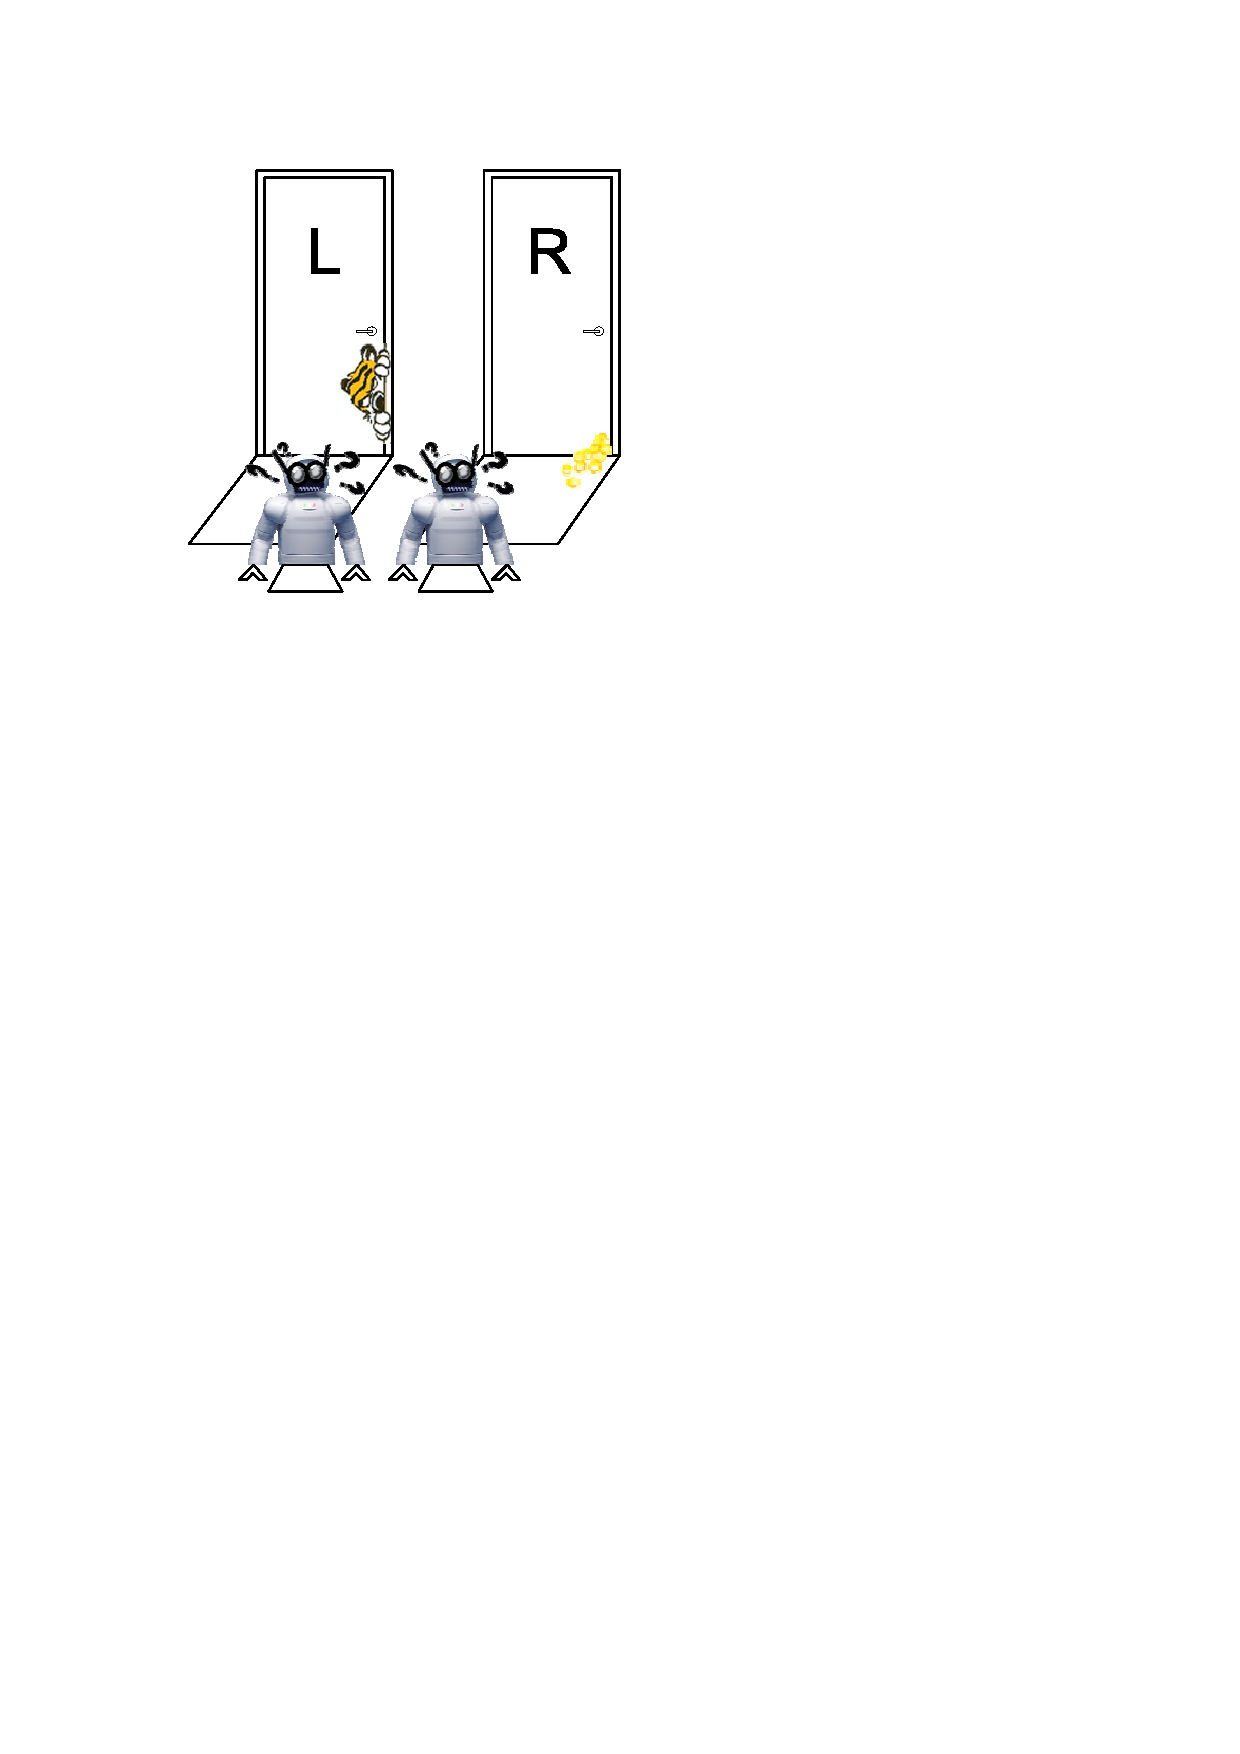
\includegraphics[width=.35\textwidth]{tiger} \caption{Le probl�me du tigre multiagent.}\label{tigerFig}
\end{figure}

Il existe donc deux �tats du monde: $\Sta = \{s_L,s_R\}$, soit le tigre est � droite, soit � gauche. Ils ont la possibilit� � chaque �tape soit d'�couter, pour tenter de d�couvrir o� se trouve le tigre, soit d'ouvrir une des deux portes ($\Act_i = \{oL,oR,Listen\}, \forall i$). Lorsqu'ils tentent d'�couter o� se trouver le tigre, ils n'ont qu'une certaine probabilit�\footnote{en g�n�ral $\Obs(o_L|s_L) = 0.85$ et pareil � droite} d'entendre le tigre derri�re la bonne porte, et le compl�mentaire\footnote{$\Obs(o_L|s_R)=0.15$ par cons�quent} � 1 d'entendre le tigre du mauvais c�t�. � partir du moment o� un des agents ouvre une porte, le jeu est r�initialis�. En ce qui concerne les r�compenses, elles se d�composent comme suit:
\begin{itemize}
  \item si les deux agents ouvrent la m�me porte, ils re�oivent une r�compense de +20 si c'est la bonne, -50 sinon;
  \item si les deux agents ouvrent chacun une porte diff�rente ils re�oivent -100;
  \item si les deux agents �coutent, une p�nalit� de -2 est inflig�e;
  \item si l'un des deux �coute alors que l'autre ouvre une porte, si celui qui ouvre se trompe, les deux agents re�oivent -101, sinon +9.
\end{itemize}

Il s'agit d'un probl�me d'observabilit� partielle simple poss�dant 2 �tats, 3 actions et 2 observations. La figure \ref{tigerStates} montre le graphe d'�tat sous-jacent ainsi que les probabilit�s de transitions et d'observations selon l'action choisie par chaque agent. Pour pouvoir planifier de mani�re optimale dans ce probl�me, il est n�cessaire pour chacun des agents de maintenir un �tat de croyance sur la position de tigre et sur la politique de l'autre agent en fonction des observations. G�n�ralement, les m�triques utilis�es dans ce probl�me consistent � calculer la r�compense obtenue apr�s un horizon $T$.

\begin{figure}[!ht]
\vspace{5pt}
\centering
\begin{tikzpicture}[line width=.1ex, scale=.65]
\begin{scope}[shape=circle,minimum size=.6cm,fill=white]
\tikzstyle{every node}=[draw] %%
\node (s1) at (0,0)  {$s_L$}; %%
\node (s0) at (5,0)  {$s_R$}; %%
\end{scope}
\draw[->,-latex] (s0.south).. controls (2.5,-2) .. (s1.south) node[near end,below=4pt]{$\la \{oL,oR\},\{oL,oR\} \ra,0.5$};  %%
\draw[->,-latex] (s1.north).. controls (2.5,2) .. (s0.north) node[near end,above=4pt]{$\la \{oL,oR\},\{oL,oR\} \ra,0.5$};  %%
\draw[->,-latex] (s1.north).. controls (0,2) and (-2,0) .. (s1.west) node[left=6pt]{$\la Listen,Listen \ra,1$};  %%
\draw[->,-latex] (s0.south).. controls (5,-2) and (7,0) .. (s0.east) node[right=6pt]{$\la Listen,Listen \ra,1$};  %%
\draw[->,-latex] (s1.north).. controls (0,2) and (-2,0) .. (s1.west) node[near start,left=6pt]{$\la \{oL,oR\},\{oL,oR\} \ra,0.5$};  %%
\draw[->,-latex] (s0.south).. controls (5,-2) and (7,0) .. (s0.east) node[near start,right=6pt]{$\la \{oL,oR\},\{oL,oR\} \ra,0.5$};  %%
\draw[->,double,-latex] (s1.south west) .. controls (-1,-1) .. (-2,-1)  node[left=6pt]{$\la Listen \Rightarrow o_L \ra,0.85$};  %%
\draw[->,double,-latex] (s0.north east) .. controls (6,1) .. (7,1)  node[right=6pt]{$\la Listen \Rightarrow o_R \ra,0.85$};  %%
\end{tikzpicture}
  \caption{Graphe d'�tat sous-jacent du probl�me du tigre.}\label{tigerStates}
\end{figure}

Concernant la difficult� de ce probl�me, elle r�side principalement dans la pr�sence d'actions \emph{�pist�miques}. Une action est dite �pist�mique d�s lors qu'elle ne modifie pas l'�tat du monde, mais agit uniquement sur l'�tat de croyance de l'agent effectuant l'action. Ces actions sont souvent d�crites comme ``observer'', ``�couter'', ``v�rifier'', etc. La difficult� du Tiger est essentiellement due � la pr�sence de ces actions, car les heuristiques habituellement utilis�es pour les \decpomdps s'av�rent inefficaces (notamment la $Q_{MDP}$).

\subsection{Domaine des d�m�nageurs}

Ce probl�me a �t� introduit dans la section~\ref{sect:demenageurs} du chapitre~\ref{chap:1} mais a �t� propos� par~\cite{SZ.07} et d�crit le comportement de deux robots d�m�nageurs qui doivent ranger des boites dans un environnement de type grille. Il y'a 3 boites dans l'environnement, deux petites et une grande. La grande n�cessite que les deux agents se coordonnent pour pouvoir la pousser. Le but est d'amener une boite (et une seule) dans la zone but (en haut de la grille, voir figure \ref{cbp3x4}). L'optimal �tant bien sur d'apporter la grosse boite dans la zone but.

\begin{figure}[!ht]
\centering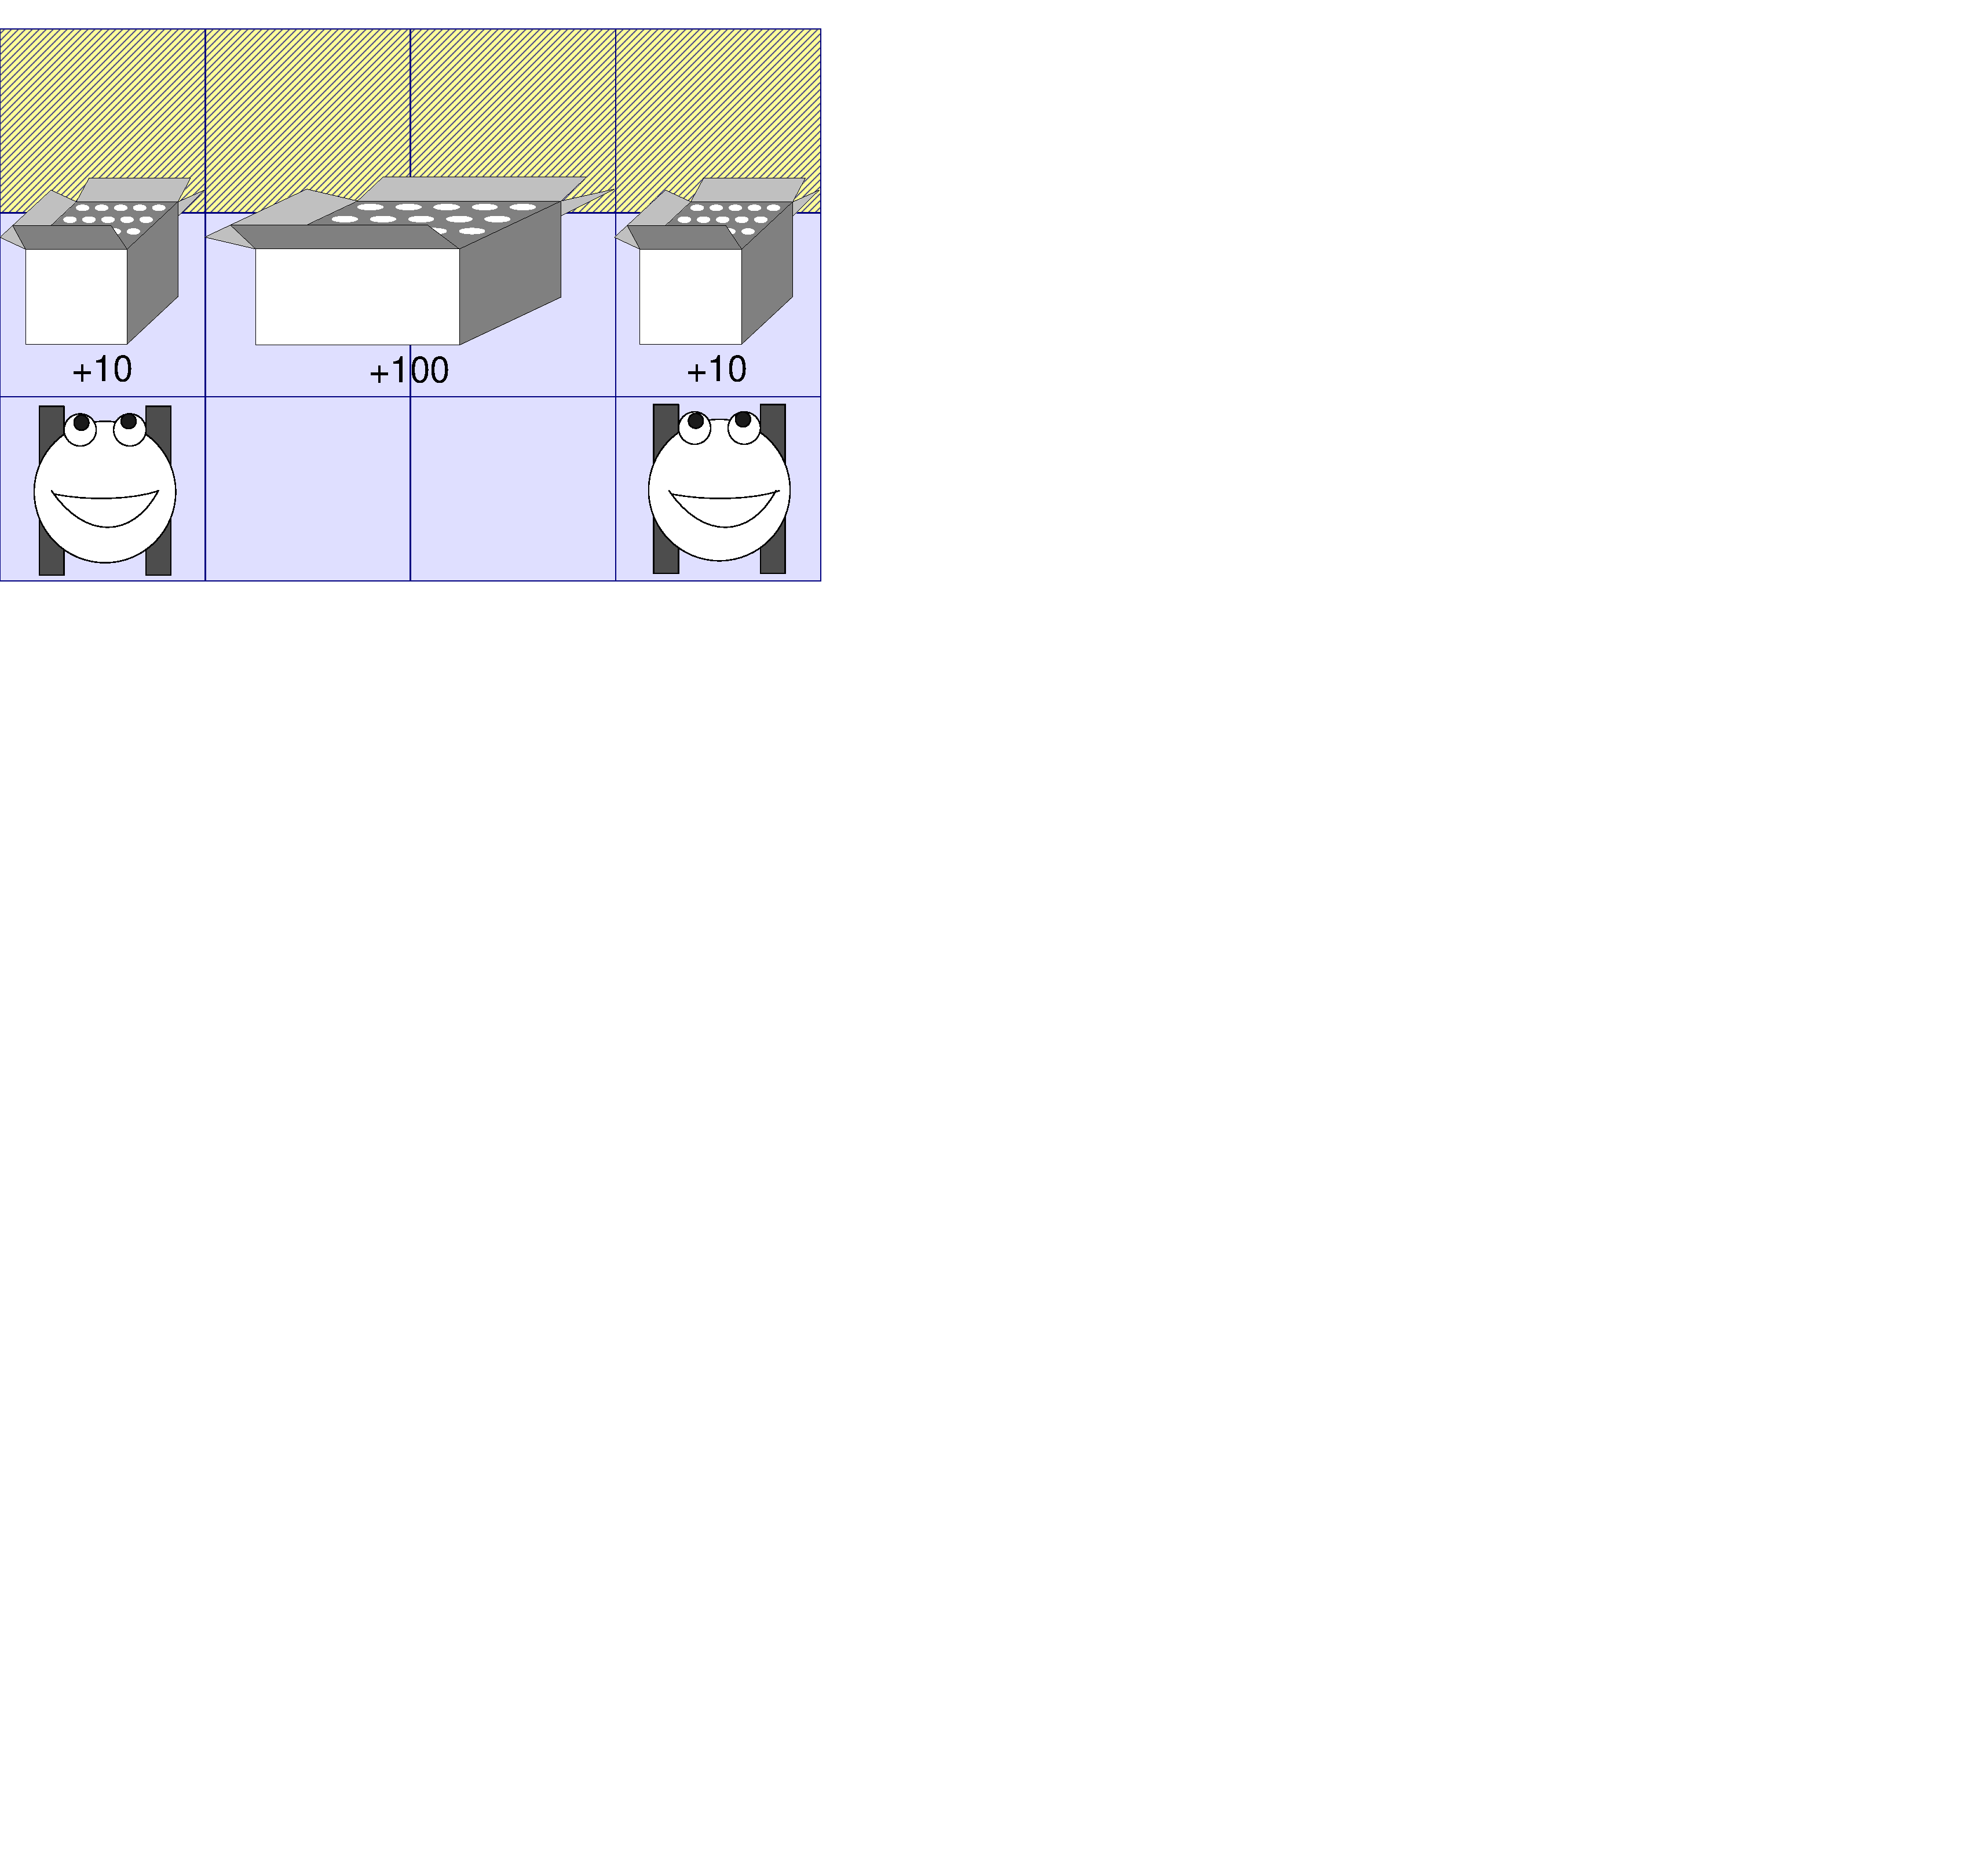
\includegraphics[width=.5\textwidth]{cbp3x4} \caption{Le probl�me du d�m�nageur en multiagent sur une grille $3\times4$.}\label{cbp3x4}
\end{figure}

Les robots ont comme possibilit� pour se d�placer d'avancer (\textsc{fwrd}), de tourner � droite (\textsc{rght}), � gauche (\textsc{left}), ou de rester sur place (\textsc{stay}). Il y'a toujours une probabilit� 0.9 que l'action r�ussisse. Dans le cas inverse, l'action \textsc{stay} est ex�cut�e. A chaque fois qu'un robot ex�cute une action, il re�oit une observation parmi les 5 suivantes : case vide, mur, autre agent, petite boite ou grande boite. La fonction de r�compense stipule que d�s qu'un agent se cogne contre une boite ou un mur, alors il re�oit +6, d�s qu'un agent pousse une petite boite dans l'en-but, chaque agent re�oit +10 et la partie est r�initialis�e. Si les deux agents poussent ensemble la grosse boite dans l'en-but, chaque agent re�oit alors +100  et la partie est aussi r�initialis�e. � chaque �tape de temps, un co�t de -1 est inflig� � chaque agent.

Ce probl�me poss�de un beaucoup plus grand nombre d'�tats que les probl�mes pr�c�dents (123 � 2 agents et dans une grille de $3\times4$). Cependant, ce probl�me reste limit� � 4 actions et 5 observations si on consid�re que les actions de l'autre agent sont totalement observables. � l'image de l'autre probl�me, la principale mesure dans celui-ci reste la valeur esp�r�e amass�e par les agents au cours du temps.

Voyons maintenant l'application de notre algorithme � ces deux probl�mes et notre comparaison avec des algorithmes similaires de la litt�rature.

\subsection{R�sultats exp�rimentaux}

Pour comparaison avec notre algorithme de Rollout d�centralis�, nous avons impl�ment� deux approches de la litt�rature pr�sent�es � la section~\ref{sect:mbdp} du chapitre~\ref{chap:2}, \textsc{imbdp}~\citep{SZ.07b} (pour \emph{Improved Memory Bounded Dynamic Programming}) et \textsc{mbdp-oc}~\citep{CZ.08} (pour \emph{Memory Bounded Dynamic Programming with Observations Compressed}), avec une l�g�re adaptation vers une version en-ligne puisque ces deux algorithmes sont initialement hors-ligne. Pour cela nous avons simplement utilis� l'algorithme~\ref{alg:simRollout} o� les lignes~\ref{alg:simRollout:agent} et~\ref{alg:simRollout:otheragents} ont �t� remplac�es par l'algorithme correspondant.

Ces algorithmes d�riv�s de \mbdp ont toutefois besoin de param�tres pr�pond�rants dans leur efficacit�. Un premier param�tre issu de \mbdp concerne le niveau d'approximation des politiques des autres agents ($maxTree$), un autre concerne le nombre d'observations $maxObs$ prises en compte lors de l'op�ration de \emph{backup} (cf. section~\ref{sect:mbdp} pour plus de d�tails). Puisque le probl�me du tigre contient seulement deux observations, nous avons choisi de ne pas approximer pour ne pas trop d�grader les performances et avons choisi de laisser $maxObs=2$. Sur le probl�me des d�m�nageurs nous avons fait varier $maxObs$ de 2 � 4. Pour le param�tre $maxTree$, nous l'avons fait varier de 3 � 7 sur le probl�me du tigre et de 2 � 5 sur le probl�me des d�m�nageurs. Aller au-del� de ces intervalles les r�sultats des algorithmes ne s'am�lioraient pas significativement en regard du temps de calcul. L'horizon de planification est �galement un param�tre important puisqu'il influence particuli�rement la r�compense accumul�e moyenne (\textsc{aar} pour \emph{accumulated average reward}). Nous avons donc choisi de laisser les algorithmes planifier pour l'ensemble de l'horizon n�cessaire. Les r�sultats report�s ci-apr�s sont ceux ayant les param�tres les plus adapt�s, i.e. apportant la meilleure r�compense accumul�e moyenne.

\begin{table}
\renewcommand\arraystretch{1.3}
\resizebox{\textwidth}{!}{
    \begin{tabular}{|c|c|c|c|c|c|c|c|c|c|c|c|c|}
      \hline
      ~ & \multicolumn{4}{c|}{online \textsc{imbdp}} & \multicolumn{4}{c|}{online \textsc{mbdp-oc}} & \multicolumn{4}{c|}{Rollout} \\
      \cline{2-13}
      $T$ & \multicolumn{2}{c|}{\textsc{atps} (ms)} & \multicolumn{2}{c|}{\textsc{aar}} & \multicolumn{2}{c|}{\textsc{atps} (ms)} & \multicolumn{2}{c|}{\textsc{aar}} & \multicolumn{2}{c|}{\textsc{atps} (ms)} & \multicolumn{2}{c|}{\textsc{aar}} \\
      \cline{2-13}
      ~ & \textsc{mlo} & \textsc{m}arg. & \textsc{mlo} & \textsc{m}arg. & \textsc{mlo} & \textsc{m}arg. & \textsc{mlo} & \textsc{m}arg. & \textsc{mlo} & \textsc{m}arg. & \textsc{mlo} & \textsc{m}arg. \\
      \hline
        5 & 39.32 & 38.87 & -65.45 & -14.96 & 40.024 & 39.48 & -41.18 & -11.9 & 138.292 & 146.8 & -50.55 & -12.4\\
        10 & 129.96 & 129.4 & -152.42 & -99.08 & 129.08 & 129.46 & -143.07 & -117.66 & 836.18 & 856.04 & -96.24 & -46.95\\
        15 & 224.17 & 227.14 & -218.9 & -214.23 & 220.07 & 216.37 & -248.69 & -193.15 & 1717.94 & 1713.25 & -193.67 & -76.36\\
      \hline
    \end{tabular}
    }
  \caption[R�sultats pour \textsc{imbdp} en-ligne,\textsc{mbdp-oc} en-ligne et dRollout dans le probl�me du Tigre.]{\textsc{imbdp} en-ligne,\textsc{mbdp-oc} en-ligne et dRollout dans le probl�me du Tigre. $maxTree = 6$ et $maxObs = 2$. \textsc{atps} est le temps moyen par �tape (\emph{average time per step}) et \textsc{aar} et la r�compense accumul�e moyenne (\emph{average accumulated reward}).}\label{resTabTig}
\end{table}

Pour les heuristiques $\Pi$ utilis�es dans l'algorithme du Rollout d�centralis�, nous avons choisi la \textsc{Qmdp} et \mbdp pour le probl�me du Tigre mais seulement le \textsc{Qmdp} dans le probl�me des d�m�nageurs pour des raisons de limites de temps dans le calcul des valeurs de chaque action jointe, mais surtout parce que le \textsc{Qmdp} est une heuristique extr�mement efficace dans tous les domaines de type grille.

Pour �valuer l'algorithme de Rollout d�centralis�, nous avons donc tout d'abord compar� sa r�compense accumul�e moyenne (\textsc{aar}) et le temps de calcul n�cessaire pour qu'il l'obtienne versus la r�compense accumul�e moyenne et le temps de calcul des deux autres algorithmes en-ligne.

\begin{figure}[htb]
\centering
\includegraphics[width=.8\textwidth]{Mat_value}
  \caption{online \textsc{imbdp}, online \textsc{mbdp-oc} and Rollout on the Tiger Problem: Average Accumulated Reward (\textsc{aar}) / horizon\label{resFigTig}}
\end{figure}

\begin{figure}[htb]
\centering
 \includegraphics[width=.8\textwidth]{Mat_time}
  \caption{online \textsc{imbdp}, online \textsc{mbdp-oc} and Rollout on the Tiger Problem: Average Time (ms) per step / horizon\label{resFigTigT}}
\end{figure}

Deux versions de chaque algorithme sont �valu�es dans les tables~\ref{resTabTig} et~\ref{resTabCoord} et dans les figures~\ref{resFigTig}, \ref{resFigTigT}, \ref{resFigCoord} et~\ref{resFigCoordT}. Les versions ``�toil�es'' (\textsc{imbdp}$^\star$, \textsc{mbdp-oc}$^\star$, Rollout$^\star$) correspondent � la mise � jour de l'�tat de croyance joint par marginalisation des observations des autres agents (cf. �quation~\eqref{eq:dRollout:marg}), alors que les versions sans �toile utilisent l'heuristique de l'observation la plus probable (cf �quation~\eqref{eq:dRollout:mlo}).

Les r�sultats rapport�s sur le probl�me multiagent du Tigre sont des moyennes sur 100 �pisodes de chacun des algorithmes. La figure~\ref{resFigTig} montre la r�compense accumul�e moyenne (\textsc{aar}) en fonction de l'horizon tandis que la figure~\ref{resFigTigT} montre le temps de calcul moyen respectif pour trouver la meilleure action � chaque �tape. Les valeurs correspondantes sont donn�es par la table~\ref{resTabTig}.

\begin{table*}
\renewcommand\arraystretch{1.3}
  \centering
\resizebox{\textwidth}{!}{
    \begin{tabular}{|c||c||c||c||c||c||c||c||c||c||c||c||c|}
      \hline
      ~ & \multicolumn{4}{c||}{online \textsc{imbdp}} & \multicolumn{4}{c||}{online \textsc{mbdp-oc}} & \multicolumn{4}{c|}{Rollout} \\
      \cline{2-13}
      $T$ & \multicolumn{2}{c||}{\textsc{atps} (ms)} & \multicolumn{2}{c||}{\textsc{aar}} & \multicolumn{2}{c||}{\textsc{atps} (ms)} & \multicolumn{2}{c||}{\textsc{aar}} & \multicolumn{2}{c||}{\textsc{atps} (ms)} & \multicolumn{2}{c|}{\textsc{aar}} \\
      \cline{2-13}
      ~ & \textsc{mlo} & \textsc{m}arg. & \textsc{mlo} & \textsc{m}arg. & \textsc{mlo} & \textsc{m}arg. & \textsc{mlo} & \textsc{m}arg. & \textsc{mlo} & \textsc{m}arg. & \textsc{mlo} & \textsc{m}arg. \\
      \hline
        5 & 5.33 & 4.54 & -3.6 & -6.8 & 13434.68 & 13426.68 & -3.5 & 5.3 & 304.67 & 301.93 & 13.4 & 11\\
        10 & 4.7 & 4.62 & -48.8 & -28.8 & 30040.33 & 30360.31 & 6.6 & 18.8 & 305.125 & 303.05 & 35.2 & 32.8\\
        15 & 4.75 & 4.59 & -59.1 & -53.4 & 58883.06 & 60925.91 & 18 & 20 & 306.18 & 305.07 & 51.6 & 51.6\\
      \hline
    \end{tabular}}
  \caption[R�sultats pour \textsc{imbdp} en-ligne,\textsc{mbdp-oc} en-ligne et dRollout dans le probl�me des d�m�nageurs.]{\textsc{imbdp} en-ligne,\textsc{mbdp-oc} en-ligne et dRollout dans le probl�me des d�m�nageurs. $maxTree = 2$ et $maxObs = 2$. \textsc{atps} est le temps moyen par �tape (\emph{average time per step}) et \textsc{aar} et la r�compense accumul�e moyenne (\emph{average accumulated reward}).}\label{resTabCoord}
\end{table*}

\begin{figure}[htb]
\centering
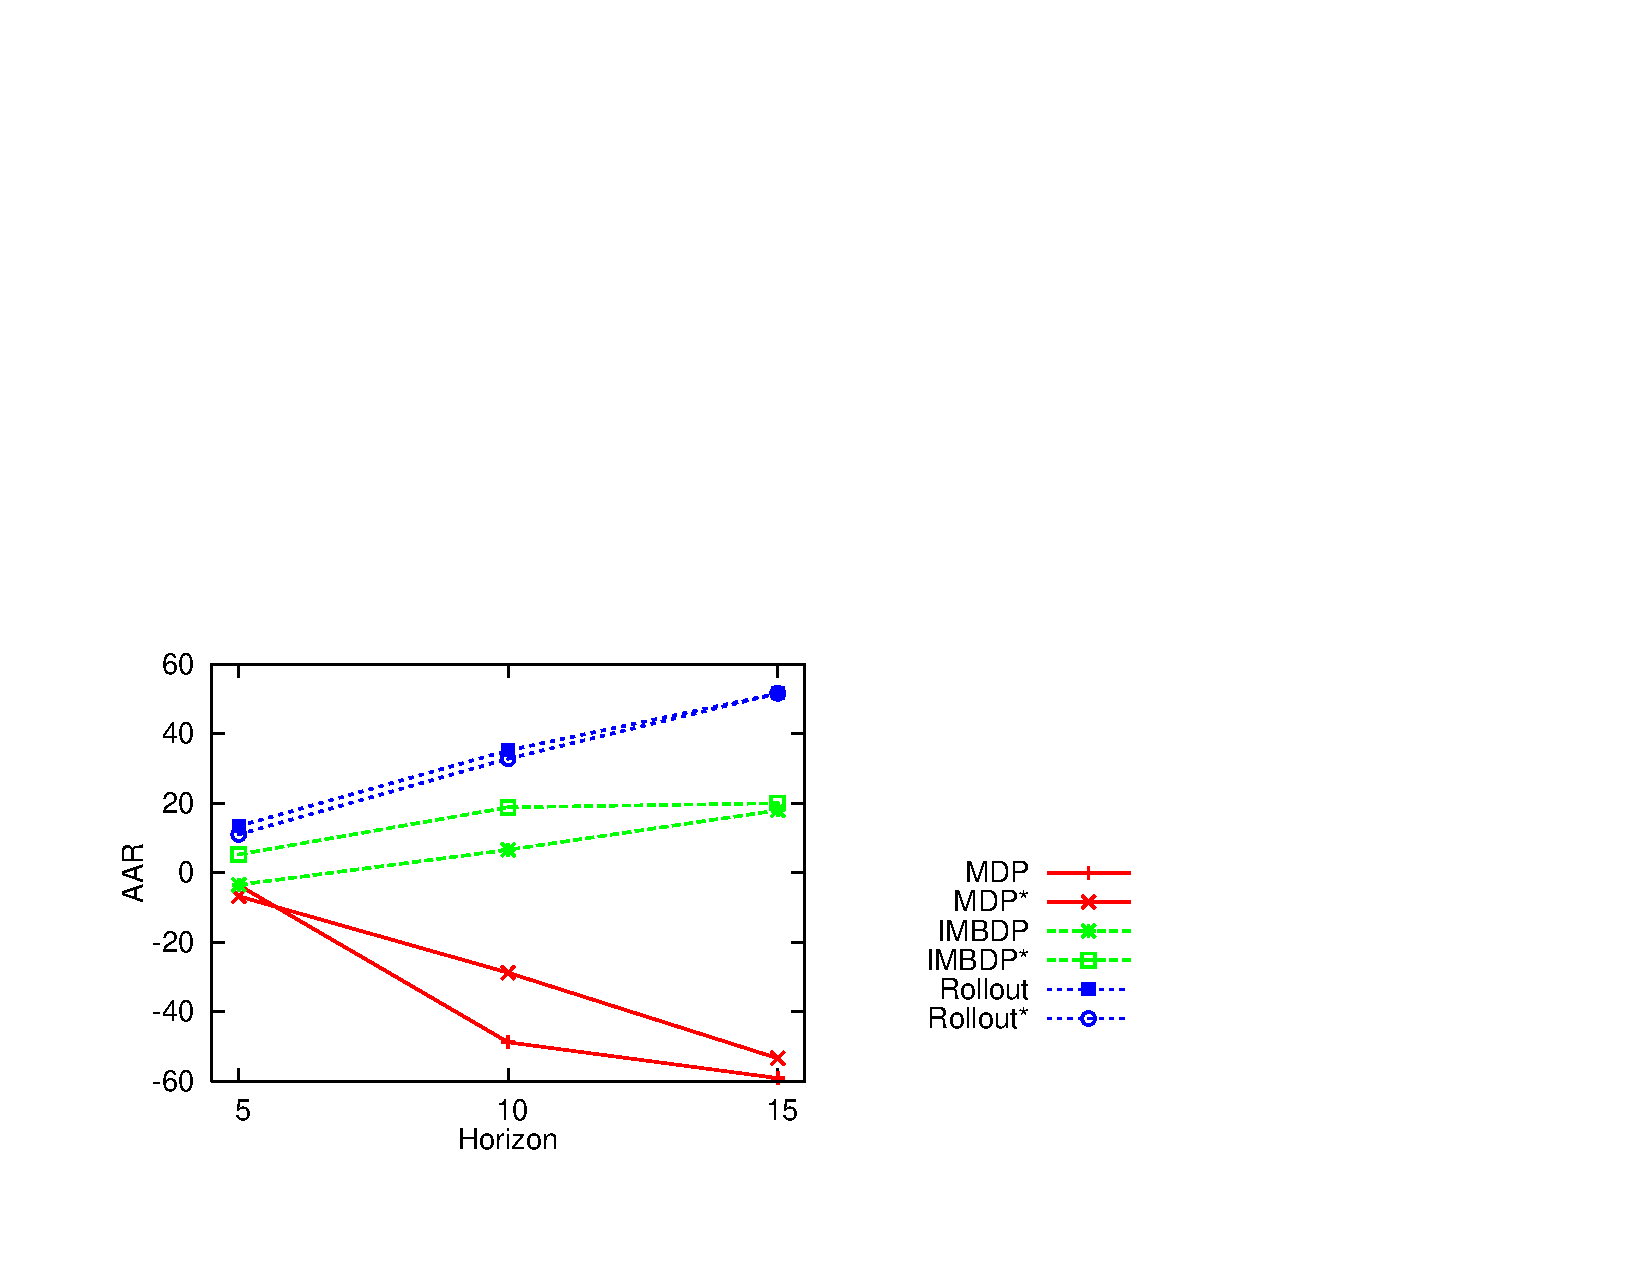
\includegraphics[width=.8\textwidth]{Coord_value}
  \caption{online \textsc{imbdp}, online \textsc{mbdp-oc} and Rollout on the Coordinate Box Pushing Problem: Average Accumulated Reward (\textsc{aar}) / horizon\label{resFigCoord}}
\end{figure}

\begin{figure}[htb]
\centering
 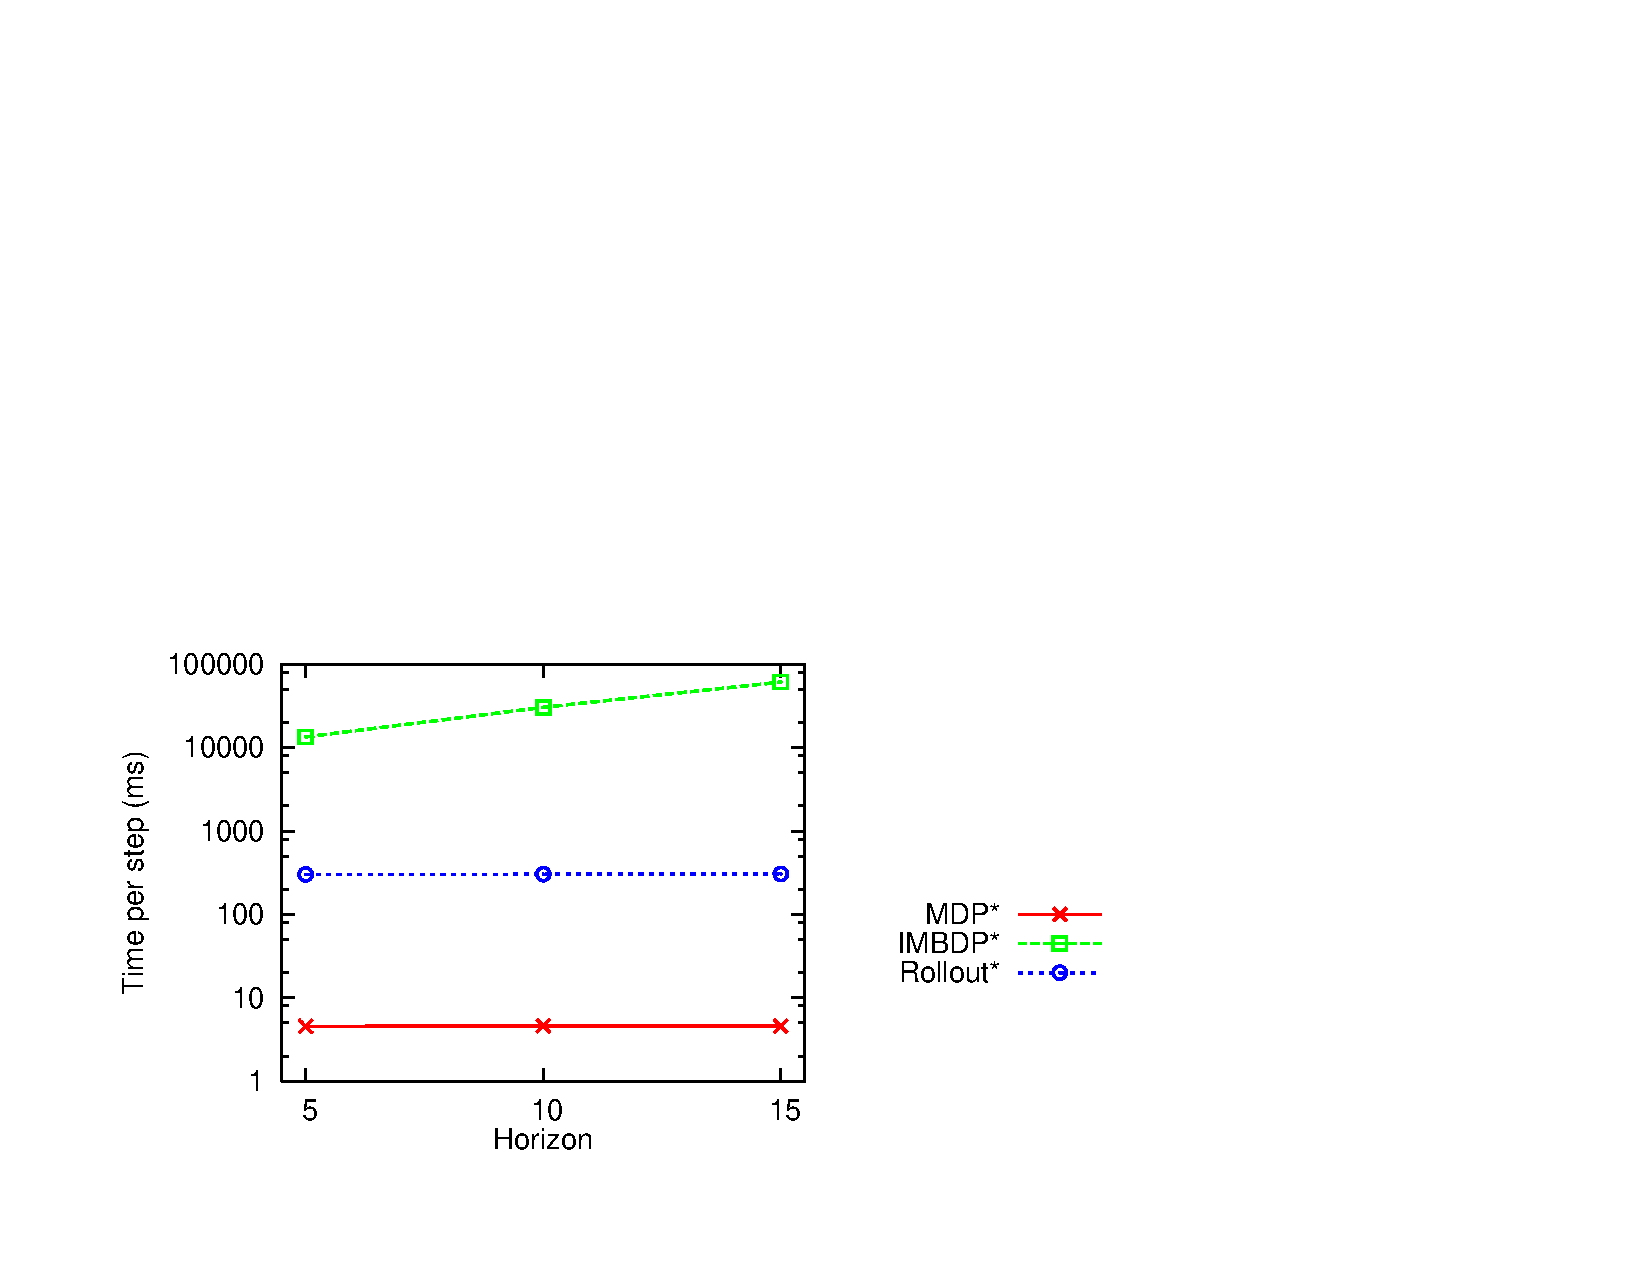
\includegraphics[width=.8\textwidth]{Coord_time}
  \caption{online \textsc{imbdp}, online \textsc{mbdp-oc} and Rollout on the Coordinate Box Pushing Problem: Average Time (ms) per step / horizon\label{resFigCoordT}}
\end{figure}

Pour les r�sultats rapport�s sur le probl�me des d�m�nageurs, 20 �pisodes de chacun des algorithmes ont �t� utilis�s pour la moyenne. Nous mettons �galement les r�sultats de l'heuristique \textsc{Qmdp} sous l'�tiquette \textsc{mdp}$^\star$. La figure~\ref{resFigCoord} montre la r�compense accumul�e moyenne en fonction de l'horion alors que la figure~\ref{resFigCoordT} montre le temps moyen n�cessaire par �tape pour calculer la meilleure action disponible. Les valeurs sont donn�es dans la table~\ref{resTabCoord}. Nous avons volontairement omis les r�sultats des algorithmes ``non-�toil�s'', i.e. ceux utilisant l'observation la plus probable pour la mise � jour de l'�tat de croyance joint, car les temps de calcul �taient �galement tr�s similaires sur ce probl�me. Ceci nous m�ne � la discussion de ces r�sultats et � la conclusion de ce chapitre.

%\begin{table*}
%\renewcommand\arraystretch{1.2}
%  \centering
%\resizebox{\textwidth}{!}{
%    \begin{tabular}{|c||c||c||c||c||c||c|}
%      \hline
%      ~ & \multicolumn{2}{c||}{\textsc{maop}} & \multicolumn{4}{c|}{Rollout} \\
%      \cline{2-9}
%      $T$ & \textsc{atps} (ms) & \textsc{aar} & \multicolumn{2}{c||}{\textsc{atps} (ms)} & \multicolumn{2}{c|}{\textsc{aar}} \\
%      \cline{2-9}
%      ~ & ~ & ~ & \textsc{mlo} & \textsc{m}arg. & \textsc{mlo} & \textsc{m}arg. \\
%      \hline
%        5 & 27.55 &  & 304.67 & 301.93 & 13.4 & 11\\
%        10 & 281.25 &  & 305.125 & 303.05 & 35.2 & 32.8\\
%        15 & 325.32 & 14.5 & 306.18 & 305.07 & 51.6 & 51.6\\
%      \hline
%    \end{tabular}}
%  \caption[R�sultats pour \textsc{maop} et dRollout dans le probl�me des d�m�nageurs.]{\textsc{maop} en-ligne et dRollout dans le probl�me des d�m�nageurs. $maxTree = 2$ et $maxObs = 2$. \textsc{atps} est le temps moyen par �tape (\emph{average time per step}) et \textsc{aar} et la r�compense accumul�e moyenne (\emph{average accumulated reward}).}\label{tab:dRollout:maop}
%\end{table*}

%Nous avons �galement compar� nos r�sultats aux travaux plus r�cents de~\cite{WZC.09} mais sans communication. Les r�sultats sont report�s dans la table~\ref{tab:dRollout:maop}. Ceci nous m�ne � la discussion de ces r�sultats et � la conclusion de ce chapitre.

\section{Discussion et conclusion}

Depuis l'apparition d'algorithmes approximatifs efficaces pour les probl�mes de la litt�rature \decpomdps, le domaine complet des algorithmes en ligne pour les \decpomdps s'est � nouveau retrouv� sous les feux de la rampe. De fait, la possibilit� de calculer des heuristiques efficientes de mani�re efficace nous a naturellement port� � proposer un algorithme de type Rollout pour les domaines de Markov d�centralis�s, o� les recherches dans de tr�s larges espaces et les mod�les dynamiques complexes sont courants.

Nous avons vu cependant qu'avec ce nouveau domaine, vient de nouveaux probl�mes, et notamment le probl�me de la maintenance d'�tat de croyance joint commun pour l'ensemble des agents du syst�me. Ce probl�me r�duit �galement � n�ant l'hypoth�se couramment utilis�e dans les \decpomdps que les agents partagent la m�me information initiale pour planifier, permettent ainsi une coordination implicite dans le calcul de la politique sur l'horizon fix�. � mesure que les agents agissent dans l'environnement, leurs �tats de croyance �voluent selon leurs observations re�ues, souvent tr�s diff�remment, induisant des probl�mes de coordination jamais rencontr�s auparavant.

Nous avons propos� dans ce chapitre deux mani�res simples de r�soudre ce probl�me sans utilisation de la communication. Une premi�re bas�e sur l'utilisation de la vraisemblance maximale des observations et une seconde bas�e sur la marginalisation des observations des autres agents dans la mise � jour de l'�tat de croyance. Nous avons alors vu que le temps de calcul �tant identique, il est pr�f�rable d'utiliser la marginalisation des observations des autres agents puisqu'elle est plus efficace dans certains cas et offre des r�sultats similaires dans d'autres.

En ce qui concerne le Rollout d�centralis�, les r�sultats montrent que cet algorithme reste adapt� aux \decpomdps d�s lors que des heuristiques adapt�es sont choisies. En fait, le Rollout utilise $|\Act|\times|\Omega|^n$ fois l'ensemble de toutes les heuristiques pour s�lectionner la meilleure action � utiliser � la prochaine �tape. Un �quilibre doit donc �tre trouv� entre le co�t de l'estimation des actions dans les �tats de croyance suivants et les r�compenses effectivement r�cup�r�es. C'est la principale raison qui nous a pouss�s � abandonner l'utilisation de \textsc{imbdp} comme heuristique sur le probl�me des d�m�nageurs. Cette heuristique co�te beaucoup trop cher pour le gain esp�r� en termes de r�compenses par rapport � l'heuristique \textsc{Qmdp} bas�e sur le \mdp sous-jacent.

Les performances de l'approche Rollout ouvrent des perspectives int�ressantes pour la recherche dans le domaine des \decpomdps. En fait, de par sa capacit� � garantir de meilleurs r�sultats que la meilleure heuristique utilis�e dans toutes les situations, le Rollout d�centralis� appara�t comme une avenue de recherche int�ressante et peu co�teuse dans certains cas pour am�liorer n'importe quelle politique sous-optimale pour les \decpomdps. Toutefois, d�s que l'heuristique devient suffisamment bonne pour donner des valeurs proches de celles de la politique optimale, la contribution du Rollout devient plus modeste puisque le co�t de l'�valuation de multiples heuristiques n'�quilibre pas l'am�lioration induite.

De fait, le Rollout est donc extr�mement bien adapt� � tous les domaines de type grille avec but fix� et sans actions �pist�miques. Le rapport/co�t qualit� de l'heuristique \textsc{Qmdp} pour ce type de probl�me est tel qu'aucune heuristique n'est plus profitable. Dans le cas de probl�mes munis d'actions �pist�miques, il est �galement possible d'utiliser l'heuristique � base d'entropie de~\cite{MRN.05} (cf. annexe~\ref{anx:it}) qui inclut le prix de l'information dans les r�compenses au travers de la r�duction d'entropie des �tats de croyance. Il est donc possible que d'autres domaines b�n�ficient �galement de ce type d'heuristiques efficaces permettant l'emploi de Rollout plut�t que d'autres algorithmes plus co�teux.

Selon notre connaissance du domaine, l'algorithme pr�sent� dans ce chapitre est le second algorithme en-ligne pour les \decpomdps. Le premier a �t� pr�sent� par~\cite{MGST.04} dans le cadre des jeux stochastiques partiellement observables. Selon~\cite{SZ.07}, leur version en-ligne de \mbdp r�alisait d�j� de meilleures performances que l'algorithme de~\cite{MGST.04} et c'est pourquoi nous ne pr�sentons pas de comparatif dans ce chapitre. D'autre part, depuis la parution de notre article~\citep{BC.08}, \cite{WZC.09} ont �galement propos� un algorithme multiagent en-ligne, mais initialement bas� sur la communication. Ils pr�sentent toutefois des r�sultats extr�mement prometteurs m�me lorsqu'aucune communication n'est disponible. Nous n'avons pas pu nous comparer � leur algorithme puisque leur mod�le d'observation et leur mod�le de r�compense dans le probl�me des d�m�nageurs ne correspondent pas exactement au mod�le que nous avons utilis�.

Comme nous l'avons �voqu� dans la section~\ref{sect:comm}, il serait donc int�ressant de voir du c�t� de la communication pour les travaux futurs. Nous avons pour cela r�alis� des travaux conjointement avec Jean-Samuel Marier~\citep{MBC.09,MBC.10} sur un probl�me de patrouille multiagent incluant la communication. Il resterait toutefois � limiter cette communication pour pouvoir comparer les algorithmes d�velopp�s aux algorithmes en-ligne multiagents existants. Nous discuterons dans le chapitre suivant plus en avant les conclusions et les perspectives de recherche de cette th�se. 


%Conclusion et travaux futurs
\chapter{Conclusions et Perspectives}
\label{chap:conclusion}

\begin{summary}
Ce chapitre rappelle tout d'abord le contexte de cette th�se et les contributions apport�es aux diff�rents domaines abord�s. Les perspectives de recherches offertes par les contributions sont ensuite d�crites et certaines sont d�taill�es au travers de quelques travaux effectu�s en collaboration avec d'autres coll�gues. Ce chapitre conclusif se termine par des remarques finales quant � l'application � des probl�mes r�els des mod�les et algorithmes pr�sent�s dans cette th�se.
\end{summary}

La prise de d�cisions dans les mod�les de Markov multiagents est particuli�rement complexe et difficile. Elle l'est �galement dans les mod�les monoagents lorsque le nombre d'�tats et/ou d'actions est particuli�rement grand. C'est pourquoi nous nous sommes int�ress�s � diff�rentes approches permettant de r�duire cette difficult� combinatoire dans les mod�les de Markov monoagents et multiagents. Dans ce contexte de r�duction de la complexit� combinatoire, nous avons propos� plusieurs m�thodes telles que l'utilisation des contraintes dans les processus d�cisionnels de Markov, la restriction de la fonction d'observation dans les processus partiellement observables ou encore la r�solution approxim�e en ligne de processus de Markov d�centralis�s. Dans cette conclusion nous allons donc rappeler les contributions de cette th�se quant � la r�duction de la complexit� combinatoire des processus de Markov avant de pr�senter quelques travaux en cours ainsi que des travaux futurs issus de ces recherches.

\section{R�sum� des contributions}

Conceptuellement, cette th�se s'est attaqu�e au probl�me de la r�duction de la complexit� combinatoire (c.f. annexe~\ref{anx:cplx}) dans les processus d�cisionnels de Markov monoagents et multiagents depuis les probl�mes les plus simples -- monoagents et compl�tement observables -- jusqu'aux probl�mes les plus complexes -- multiagents et partiellement observables. Dans une premi�re partie (au chapitre~\ref{chap:3}) nous avons r�duit la complexit� inh�rente aux \mdps lorsqu'un grand nombre d'actions sont possibles sous certaines contraintes difficiles � repr�senter dans le mod�le \mdp initial~\citep{BC.07,BPC.07}. Dans une seconde partie (au chapitre~\ref{chap:4}) nous nous sommes attaqu�s au probl�me de la repr�sentation de la fonction d'observation trop g�n�rale et avons donc propos� une sous-classe d'observabilit� permettant de r�duire consid�rablement la complexit� en pire cas dans les cas monoagent et multiagent~\citep{BC.09,BC.10,BC.10a}. Enfin, nous avons propos� au chapitre~\ref{chap:5} un algorithme en ligne de planification pour les mod�les multiagents partiellement observables lorsqu'aucune communication n'est possible~\citep{BC.08}. Voyons donc rapidement un r�sum� de ces contributions et les diff�rentes compl�mentarit�s entre ces parties.

\begin{description}
\item[R�duction de l'espace de recherche par des contraintes sur les actions:] Cet-te contribution sugg�re l'utilisation des repr�sentations � base de contraintes pour la r�solution de probl�mes d'allocation de ressources sous diff�rents types de contraintes. L'id�e consiste � utiliser un algorithme permettant de dissocier la r�solution des contraintes des allocations aux ressources et la r�solution du probl�me s�quentiel de planification dans un mod�le unifi�. Un algorithme en ligne adapt� � cette dissociation a �galement �t� propos� offrant ainsi des gains en performance significatifs sur un probl�me de d�fense navale.
\item[R�duction de l'incertitude par des contraintes sur les observations:] C'est en commen�ant par l'extension du mod�le d�terministe partiellement observable que nous avons propos� une nouvelle classe sp�cifique d'observabilit� assurant la convergence en probabilit� de l'�tat de croyance vers un �tat sp�cifique. Cette contribution s'aligne �galement dans la direction de la r�duction combinatoire des probl�mes de Markov, mais dans le cas partiellement observable. Elle permet notamment de comprendre plus pr�cis�ment quel est l'effet de l'observabilit� dans la complexit� des mod�les partiellement observables tout en ouvrant la porte � d'autres chercheurs en vue d'induire une heuristique admissible.
\item[R�solution en ligne de probl�mes d�centralis�s:] Un algorithme de r�solution en ligne de \decpomdps ne faisant aucune hypoth�se sur la communication ou l'interaction des agents \emph{a priori} a �t� propos� dans ce cadre. Nous avons vu qu'un tel algorithme est difficilement applicable sans communication et que de mauvaises d�cisions locales peuvent �ventuellement conduire � des r�sultats globaux catastrophiques. Il convient toutefois de mod�rer ces propos dans la mesure ou peu de probl�mes r�els sont aussi coupl�s que le sont les probl�mes ``jouets'' sur lesquels sont effectu�es la majorit� des exp�rimentations. Des travaux en ce sens seront pr�sent�s dans la section suivante.
\end{description}

En r�sum�, cette th�se vise � contribuer � la r�duction combinatoire des mod�les de Markov et � l'�tude de l'observabilit� dans de tels mod�les. Une certaine compl�mentarit� ressort des contributions de cette th�se puisque chacune de ces contributions s'attaque � un probl�me distinct des mod�les de Markov. On peut ainsi imaginer regrouper ces contributions dans un mod�le multiagent unique et unifi� associant les contraintes sur les actions, l'observabilit� bijective et autorisant la communication implicite � des fins de synchronisation. Voyons donc maintenant le cadre des perspectives de recherche d�coulant des contributions de cette th�se.

\section{Perspectives de recherche}

Cette th�se peut �tre �tendue dans diverses directions.  Dans ce contexte, cette section d�crit bri�vement les perspectives de recherches associ�es � chaque approche d�velopp�e dans ce manuscrit avant de pr�senter une application du mod�le rassemblant toutes les contributions ci-avant.

\subsection{Multiagent \pac{m}a\pac{csp}}

Bri�vement discut�e dans la conclusion du chapitre~\ref{chap:3}, l'extension au cas multiagent des probl�mes de Markov de satisfaction de contraintes permettrait �ventuellement une plus grande expressivit� du mod�le tout en assurant une r�duction combinatoire encore plus grande que le mod�le monoagent propos�. En effet, on peut supposer qu'un tel mod�le permettrait de mod�liser certains types d'interactions sp�cifiques existant entre les agents tels que les interactions n�gatives par exemple. Il est possible que des agents se trouvent dans l'impossibilit� de r�aliser une action de par la pr�sence d'un autre agent ou de par l'action d'un autre agent � une �tape pr�c�dente. Ce type d'interactions se repr�sente tr�s bien � l'aide de contraintes et permettrait ainsi �galement de r�duire l'espace des actions jointes disponibles lors de la recherche d'une solution. Les contraintes sont donc un bon moyen de repr�senter certaines interactions entre les agents en vue de r�duire la complexit� d'algorithmes d�j� existants.

\subsection{�tude des mod�les � observabilit� bijective et transition stochastique}

Nous nous sommes limit�s, dans le chapitre~\ref{chap:4}, � l'�tude des mod�les � transition d�terministes m�me si des travaux pr�liminaires concernant les fonctions de transitions stochastiques sont rapport�s dans l'annexe~\ref{anx:it}. Poursuivre ces travaux en �tudiant � la fois la structure de la fonction de transition et le bruit g�n�r� par celle-ci est �galement une perspective de recherche int�ressante. Il serait ainsi possible de relier les travaux propos�s � ceux de~\cite{HLR.07} puisque ces auteurs ont �tudi� certaines fonctions de transitions permettant l'approximation de \pomdps. Les auteurs ont en effet r�ussi � montrer qu'il existe des classes de probl�mes dont le nombre d'�tats de croyance accessible depuis un �tat de croyance donn� est fini. Ainsi, il suffit de faire une it�ration de valeur sur cet ensemble fini d'�tats de croyance pour trouver une politique optimale pour le \pomdp � horizon infini.

Il est �galement possible d'�tendre nos travaux sur la bijectivit� des observations aux \pomdps continus o� la fonction d'observation est une fonction bijective exacte sur laquelle un bruit gaussien est ajout�. Il serait ainsi possible de d�finir une bijectivit� de la transition aussi appel�e r�versibilit� de la matrice de transition dans les mod�les usuels de Markov en math�matiques~\citep{AF.02}. Ces aspects seront abord�s dans la section~\ref{sect:gppomdp} de ce chapitre qui d�crit des travaux entrepris en collaboration avec Patrick Dallaire sur les \pomdps a espaces continus~\citep{DBRC.09}.

\subsection{Utilisation de la communication pour la synchronisation des �tats de croyance}

Une autre avenue de recherche int�ressante apport�e par l'observabilit� bijective concerne la communication dans les syst�mes multiagents. Dans l'exemple multiagent de cha�ne de seaux d'eau trait� dans le chapitre~\ref{chap:4}, pour que les agents aient acc�s � l'�tat complet du syst�me, nous avons fait l'hypoth�se que les agents pouvaient communiquer, comme bon leur semblait, la partie de l'�tat non visible par un autre agent. Nous n'avons cependant fait aucune hypoth�se quant � la qualit� de cette communication qui peut ainsi �tre bruit�e. Ce type de communication partielle, en dehors des sch�mas classiques de communication dans les travaux actuels dans le domaine des \decpomdps, devrait �tre compar� aux algorithmes faisant l'hypoth�se que la communication sert � synchroniser l'�tat de croyance des agents en communiquant l'historique des actions et observations, tels que pr�sent�s au chapitre~\ref{chap:5}. On pourrait alors imaginer une forme de communication efficace et s�mantiquement non redondante dans des espaces factoris�s et structur�s et ainsi r�duire les co�ts associ�s � la communication.

\section{Un mod�le unifi� appliqu� � la patrouille d'un espace repr�sent� sous forme de graphe}

C'est dans le cadre de la ma�trise de Jean-Samuel Marier que nous avons essay� de mettre en pratique les approches propos�es dans cette th�se~\citep{MBC.09,MBC.10}. Un mod�le multiagent pour le probl�me de patrouille d'agents autonomes a donc �t� propos� sur la base des principes suivants:
\begin{itemize}
\item Les agents sont contraints dans leurs actions par un graphe de localisations � surveiller aussi souvent que possible;
\item Les agents observent avec certitude leur position et communiquent celle-ci aux autre agents;
\item Les agents peuvent communiquer leur �tat local et leur politique locale inaccessible aux autres agents avec une fr�quence suffisamment �lev�e telle que les d�lais ou la fiabilit� du r�seau de communication ne puissent pas �tre mise en cause;
\item Les agents n'ont pas acc�s � l'information qu'ils surveillent, ils n'ont qu'une repr�sentation probabiliste (un �tat de croyance) de l'�tat de fra�cheur de l'information qu'ils cherchent � surveiller. Ainsi, dans le cadre de la surveillance de for�ts pour la d�tection d'incendie par exemple, les agents pourraient �tre munis de capteurs infrarouges d�tectant avec une certaine probabilit� un feu � une position donn�e, mais il n'auront aucune confirmation de la part de ce capteur si quelque chose a �t� d�couvert ou pas. Cela permet un niveau d'abstraction suppl�mentaire et ainsi de d�coupler la t�che de surveillance avec l'objet � surveiller. On peut ainsi supposer avoir le mod�le des capteurs sp�cifiques � utiliser sans savoir exactement quels sont ces capteurs ou � quoi ils servent.
\end{itemize}

Il a donc �t� propos� un mod�le~\citep{MBC.09} pour ce probl�me bas� sur un m�lange de processus de Markov multiagents partiellement observables et de processus semimarkoviens g�n�ralis�s~\citep{Y.04} incluant la prise en compte du temps continu et la gestion d'�v�nements concurrents. Nous le d�taillerons rapidement dans cette section. Le lecteur int�ress� par sa r�solution est invit� � se r�f�rer � la ma�trise de~\cite{M.10}.

\subsection{Formalisation du probl�me de patrouille}
\newcommand\noeud{n\oe ud\xspace}
\newcommand\noeuds{n\oe uds\xspace}

Comme nous l'avons �nonc� plus haut, le probl�me de patrouille est contraint et structur� par un graphe. Ainsi, les agents ne peuvent se rendre d'une position � une autre que si une ar�te du graphe existe entre ces deux n\oe uds. Appelons $V$ l'ensemble des \noeuds et $E$ l'ensemble des ar�tes. Soit $L$ une matrice de taille $|V| \times |V|$, dans laquelle $L_{ij}$ est un nombre r�el \emph{non-n�gatif} qui repr�sente le temps requis pour aller d'un \noeud $i$ � un \noeud $j$ si l'ar�te $[i,j]$ appartient � $E$; $L_{ij}$ est infini sinon. Dans un cas plus g�n�ral, $L_{ij}$ est une distribution de probabilit� sur le temps. Chaque \noeud a un poids d'importance $w_i$. On d�notera par $\mathbf{w}$ le vecteur de tous les poids. Lorsque l'on suppose que toutes les positions sont accessibles depuis n'importe laquelle position, alors le graphe est complet.

La mesure de performance habituellement utilis�e dans la litt�rature sur le probl�me de patrouille est l'\emph{oisivet�}. L'oisivet� d'un sommet $i$, not�e $\tau_i$ repr�sente le temps �coul� depuis la derni�re visite d'un agent � ce sommet. L'oisivet� est 0 lorsqu'un agent est sur le sommet et \mbox{$\tau_i^{t+\Delta t} = \tau_i^t + \Delta t$} si le sommet n'a pas eu de visite dans l'intervalle de temps $(t, t+\Delta t)$. Parce que l'oisivet� est une quantit� non born�e, nous avons d�cid� d'utiliser ce que nous avons appel� la \emph{fra�cheur} d'un sommet. La fra�cheur d'un sommet $i$ est donn� par $k_i^t = b^{\tau_i^t}$, avec $0 < b < 1$. Ainsi, $k_i^t$ est toujours compris entre 0 et 1 et peut �tre vue comme la valeur esp�r�e d'un variable al�atoire de Bernoulli qui vaut 1 lorsque le sommet $i$ est correctement observ� par l'argent en patrouille et 0 sinon. De fait, $k_i^t$ est la probabilit� que cette variable soit 1 au temps $t$. L'id�e d'observer ``correctement'' reste g�n�rale comme expliqu�e au quatri�me point de l'introduction de cette section. Ainsi, au temps $t$, $k_i^t$ est la probabilit� que l'agent ait r�ussi � observer ce qu'il avait � observer � la position $i$. La mesure de performance $k_i^t$ est ensuite calcul�e en faisant la somme pond�r�e par la valeur des sommets $\mathbf{w}$ du vecteur $\mathbf{k}^t$.

Cette probabilit� �volue de la mani�re suivante : $k_i^{t+\Delta t} = k_i^t b^{\Delta t}$ si aucune visite n'a eu lieu dans l'intervalle de temps  $(t, t + \Delta t)$. Si un agent avec des observations bruit�es visite le sommet $i$ au temps $t$, l'oisivet� devient alors 0 avec probabilit� $(1-a)$, o� $a$ satisfait $b < (1-a) \leq 1$. Si $n$ agents visitent le sommet simultan�ment au temps $t+\Delta t$ et qu'il n'y eu aucune visite depuis le temps $t$, alors on peut �crire:
\begin{equation}
\label{eq:update-k}
k_i^{t+\Delta t} = k_i^t a^n b^{\Delta t} + 1 - a^n.
\end{equation}

En r�sum�, une instance du probl�me de patrouille est un tuple \mbox{$\langle L, \mathbf{w}, a, b \rangle$} constitu� de $(i)$ la matrice $L$ des longueurs des ar�tes, $(ii)$ du vecteur $\mathbf{w}$ des poids des sommets, et $(iii)$ des param�tres $a$ et $b$ repr�sentant respectivement la probabilit� que l'oisivet� ne soit pas remise � 0 lorsqu'un agent passe par un sommet et le taux de d�croissance de $k_i$ au cours du temps, ou encore la rapidit� de l'obsolescence de l'information au sommet $i$. Il convient ici de remarque que $b$ peut �tre diff�rent d'un sommet � l'autre et que $a$ peut �tre diff�rent pour chaque pair d'agent/sommet. Nous n'utiliserons toutefois qu'un seul param�tre $a$ et $b$ pour des raisons de clart�.

\subsection{Repr�sentation par un \pac{mmdp} en temps discret}

En utilisant les capacit�s de communication �voqu�es pr�c�demment, il est possible de repr�senter ce probl�me sous la forme d'un \mmdp (c.f. chapitre~\ref{chap:2}) o� l'�tat des agents est compl�tement observable, mais hybride. Tous les agents ont effectivement la m�me information compl�te quant � la position des autres agents et l'�tat (incertain et continu) des sommets du graphe, pour pouvoir prendre une d�cision coordonn�e. Du fait que les actions peuvent avoir des dur�es diff�rentes et ainsi d�synchroniser les agents, il est n�cessaire d'�tendre ce mod�le au temps continu avec la gestion �v�nementielle d'actions concurrentes. Cette gestion se fait tr�s bien dans les processus d�cisionnels semi-markoviens g�n�ralis�s (\textsc{gsmdp}~\citep{Y.04}) que nous ne d�taillerons pas ici.

L'�tat se d�compose alors en plusieurs variables, certaines d�crivant les positions de chacun des agents, d'autres mod�lisant la fra�cheur de chacun des sommets. Ainsi, si $N$ agents sont dans l'environnement, le nombre d'�tats possible est de
\begin{equation}
\mathcal{S} = V^N \times \left[0, 1\right]^{|V|} \label{eq:state-space}.
\end{equation}
�tant donn� un �tat \mbox{$s = \left(\mathbf{v}, \mathbf{k}\right)\in \mathcal{S}$}, $v_i$ est la position de l'agent $i$ et $k_i$ est l'oisivet� du sommet $i$. Nous utilisons \mbox{$s^t = \left(\mathbf{v}^t, \mathbf{k}^t\right)$} pour l'�tat et ses composantes � l'instant $t$.

A certains instants, appel�s �tapes de d�cision, les agents doivent choisir une action. Tous les agents doivent �tre en train d'effectuer une action � chaque instant et ne peuvent changer d'action que lorsqu'ils sont � une �tape de d�cision. Les actions sont contraintes par la structure du graphe et sa position: si un agent est dans un sommet $v$, il ne peut choisir son action que parmi \mbox{$\mathcal{A}_v = \left\{ u : [v, u] \in E \right\}$}. Si un agent choisit l'action $u$ depuis le sommet $v$ au temps $t^i$, la prochaine �tape de d�cision surviendra au temps \mbox{$t^{i+1} = t^i + L_{vu}$}, et $v^t = v$ tant que $t \in [t^i, t^{i+1})$ et $v^t = u$ d�s que $t = t^{i+1}$. En d'autres mots, l'agent est consid�r� comme �tant � son sommet de d�part pendant tout le trajet, et ce, jusqu'� ce qu'il arrive. Si $L_{vu}$ est une distribution de probabilit� sur le temps d'arriv�e, alors $t^{i+1}$ en est une aussi �tant donn� $t^i$.

Du fait que les agents n'agissent plus n�cessairement de mani�re synchronis�e, les actions deviennent alors concurrentes et peuvent s'entrem�ler arbitrairement puisque chaque composante $k_i$ de $\mathbf{k}$ �volue ind�pendamment des autres. On peut alors r��crire l'�quation~\eqref{eq:update-k} de telle sorte � prendre en compte cette concurrence des actions en temps discret. Soit $\{ t^j \}_j$ une s�quence d'�tapes de d�cisions et $n_i^j$ le nombre d'agents arrivant au sommet $i$ au temps $t^j$. Si l'on d�note $\Delta t^j = t^{j+1} - t^j$, on peut r��crire l'�quation~\eqref{eq:update-k}:
\[
k_i^{t^{j+1}} = k_i^{t^j} a^{n_i^{j+1}} b^{\Delta t^j} + 1 - a^{n_i^{j+1}}.
\]

Les r�compenses $R$ sont alors calcul�es en fonction du vecteur $\mathbf{k}$. Plus sp�cifiquement, le gain en r�compense est donn� par la somme pond�r�e des $k_i$ par les $w_i$ et la fonction de valeur du \textsc{gsmdp} est alors calcul�e de la mani�re suivante:
\begin{equation}
V^\pi(s)
	\underset{(a)}{=}
		\Esp{ \int_0^\infty \gamma^t  \mathbf{w}^\top\mathbf{k}^t \, dt. }
	\underset{(b)}{=}
		\Esp{
			\sum_{j=0}^\infty \gamma^{t^j} \mathbf{w}^\top\mathbf{k}^{t^j}
				\frac{(b\gamma)^{\Delta t^j} - 1}{\ln(b\gamma)}
		}
\label{eq:value}
\end{equation}
O� $\gamma \in (0, 1]$ est le facteur d'escompte.

Il convient de pr�ciser que l'�galit� $(a)$ est donn�e par la d�finition d'une fonction de valeur � temps continu, et $(b)$ est obtenue par l'int�gration par morceaux entre les diff�rentes �tapes de d�cisions. En outre, l'esp�rance est prise ici sur la dur�e stochastique des actions. La s�quence d'�tats rencontr�s d�pend des actions choisies par les agents repr�sent�es par leur politique $\pi$. Le probl�me �tant de trouver la politique maximisant cette valeur. Plusieurs algorithmes ont �t� propos�s par~\cite{M.10}. Des exemples de graphes sont donn�s par les figures~\ref{fig:instances} et~\ref{fig:random-instances}.

\begin{figure}
\centering
\subfigure[Wheel]{\resizebox{.3\textwidth}{!}{\begin{tikzpicture}[scale=2.5]
	\tikzstyle{vertex}=[circle,draw=black,minimum size=1mm,inner sep=1pt]

	\node [vertex] (9)									{};
	\node [vertex] (1) [right of=9,fill=black]			{};
	\node [vertex] (2) [above right of=9]				{};
	\node [vertex] (3) [above of=9]						{};
	\node [vertex] (4) [above left of=9]				{};
	\node [vertex] (5) [left of=9]						{};
	\node [vertex] (6) [below left of=9]				{};
	\node [vertex] (7) [below of=9]						{};
	\node [vertex] (8) [below right of=9]				{};

		\path	(1)	edge (2)	edge (9)
		(2)	edge (3)
		(3)	edge (4)	edge (9)
		(4)	edge (5)
		(5)	edge (6)	edge (9)
		(6)	edge (7)
	(7)	edge (8)	edge (9)
		(8)	edge (1);
\end{tikzpicture}
}}
\;
\subfigure[Cloverleaf]{\resizebox{.3\textwidth}{!}{\begin{tikzpicture}[scale=2.5]

	\tikzstyle{vertex}=[circle,draw=black,node distance=7mm,minimum size=1mm,inner sep=1pt]

	\node [vertex] (0) [fill=black]			{};
	\node [vertex] (1) [right of=0]			{};
	\node [vertex] (2) [above right of=1]	{};
	\node [vertex] (3) [below right of=1]	{};
	\node [vertex] (4) [left of=0]			{};
	\node [vertex] (5) [above left of=4]	{};
	\node [vertex] (6) [below left of=4]	{};
	\node [vertex] (7) [above of=0]			{};
	\node [vertex] (8) [above right of=7]	{};
	\node [vertex] (9) [above left of=7]	{};

	\node at (0) [below=1mm,font=\footnotesize] {0};

		\path	(0)	edge (1) edge (4) edge (7)
		(1)	edge (2) edge (3)
		(2)	edge (3)
		(4)	edge (5) edge (6)
		(5)	edge (6)
	(7) edge (8) edge (9)
		(8) edge (9);
\end{tikzpicture}
}}
\;
\subfigure[Cuboctahedron]{\resizebox{.3\textwidth}{!}{\begin{tikzpicture}[scale=.4]
\tikzstyle{vertex}=[circle,draw=black,node distance=2mm,minimum size=1mm,inner sep=1pt]
\node [vertex] (0) at(-2.5,2.5) [fill=black] {};
\node [vertex] (1) at(2.5,2.5) {};
\node [vertex] (2) at(0,1.5) {};
\node [vertex] (3) at(-0.5,0.5) {};
\node [vertex] (4) at(0.5,0.5) {};
\node [vertex] (5) at(-1.5,0) {};
\node [vertex] (6) at(1.5,0) {};
\node [vertex] (7) at(-0.5,-0.5) {};
\node [vertex] (8) at(0.5,-0.5) {};
\node [vertex] (9) at(0,-1.5) {};
\node [vertex] (10) at(-2.5,-2.5) {};
\node [vertex] (11) at(2.5,-2.5) {};

\path (0) edge (1);
\path (0) edge (2);
\path (0) edge (5);
\path (0) edge (10);
\path (1) edge (2);
\path (1) edge (6);
\path (1) edge (11);
\path (2) edge (3);
\path (2) edge (4);
\path (3) edge (4);
\path (3) edge (5);
\path (3) edge (7);
\path (4) edge (6);
\path (4) edge (8);
\path (5) edge (7);
\path (5) edge (10);
\path (6) edge (8);
\path (6) edge (11);
\path (7) edge (8);
\path (7) edge (9);
\path (8) edge (9);
\path (9) edge (10);
\path (9) edge (11);
\path (10) edge (11);
\end{tikzpicture}
}}
\\
\subfigure[Map-A]{\resizebox{.45\textwidth}{!}{\begin{tikzpicture}[-,auto]
\tikzstyle{vertex}=[circle,draw=black,node distance=7mm,minimum size=1mm,inner sep=1pt]
\node [vertex] (0) at(0,0) [fill=black] {};
\node [vertex] (1) at(0.65,-0.00) {};
\node [vertex] (2) at(1.40,-0.00) {};
\node [vertex] (3) at(1.92,-0.00) {};
\node [vertex] (4) at(3.19,-0.00) {};
\node [vertex] (5) at(3.66,-0.01) {};
\node [vertex] (6) at(0.00,-0.73) {};
\node [vertex] (7) at(0.00,-1.19) {};
\node [vertex] (8) at(0.00,-1.50) {};
\node [vertex] (9) at(0.00,-1.91) {};
\node [vertex] (10) at(0.00,-2.76) {};
\node [vertex] (11) at(0.65,-0.64) {};
\node [vertex] (12) at(1.40,-0.73) {};
\node [vertex] (13) at(1.92,-0.47) {};
\node [vertex] (14) at(3.19,-0.47) {};
\node [vertex] (15) at(3.66,-0.40) {};
\node [vertex] (16) at(4.48,-0.40) {};
\node [vertex] (17) at(4.78,-0.15) {};
\node [vertex] (18) at(2.78,-0.73) {};
\node [vertex] (19) at(1.92,-0.94) {};
\node [vertex] (20) at(1.92,-1.19) {};
\node [vertex] (21) at(1.07,-1.19) {};
\node [vertex] (22) at(1.48,-1.50) {};
\node [vertex] (23) at(1.16,-1.91) {};
\node [vertex] (24) at(2.46,-1.19) {};
\node [vertex] (25) at(2.46,-1.50) {};
\node [vertex] (26) at(2.46,-1.66) {};
\node [vertex] (27) at(1.80,-1.91) {};
\node [vertex] (28) at(1.49,-2.23) {};
\node [vertex] (29) at(1.07,-2.37) {};
\node [vertex] (30) at(1.07,-2.63) {};
\node [vertex] (31) at(0.32,-3.00) {};
\node [vertex] (32) at(4.48,-0.62) {};
\node [vertex] (33) at(3.66,-0.62) {};
\node [vertex] (34) at(3.71,-0.94) {};
\node [vertex] (35) at(4.48,-1.35) {};
\node [vertex] (36) at(3.71,-1.19) {};
\node [vertex] (37) at(3.94,-1.50) {};
\node [vertex] (38) at(3.54,-2.05) {};
\node [vertex] (39) at(2.46,-2.28) {};
\node [vertex] (40) at(3.95,-1.66) {};
\node [vertex] (41) at(1.48,-2.86) {};
\node [vertex] (42) at(2.22,-2.86) {};
\node [vertex] (43) at(2.66,-3.00) {};
\node [vertex] (44) at(4.79,-3.00) {};
\node [vertex] (45) at(4.04,-2.45) {};
\node [vertex] (46) at(4.13,-1.98) {};
\node [vertex] (47) at(5.00,-2.30) {};
\node [vertex] (48) at(5.00,-1.68) {};
\node [vertex] (49) at(5.00,-1.43) {};
\path (0) edge (1);
\path (0) edge (6);
\path (1) edge (2);
\path (1) edge (11);
\path (10) edge (23);
\path (10) edge (29);
\path (10) edge (31);
\path (11) edge (12);
\path (12) edge (19);
\path (12) edge (21);
\path (12) edge (13);
\path (13) edge (18);
\path (13) edge (19);
\path (14) edge (15);
\path (14) edge (18);
\path (14) edge (33);
\path (15) edge (16);
\path (15) edge (17);
\path (15) edge (33);
\path (16) edge (17);
\path (16) edge (32);
\path (18) edge (19);
\path (18) edge (33);
\path (18) edge (34);
\path (19) edge (20);
\path (19) edge (21);
\path (2) edge (12);
\path (2) edge (13);
\path (2) edge (3);
\path (20) edge (21);
\path (20) edge (22);
\path (20) edge (24);
\path (21) edge (22);
\path (21) edge (26);
\path (22) edge (23);
\path (22) edge (25);
\path (22) edge (27);
\path (23) edge (27);
\path (23) edge (28);
\path (23) edge (29);
\path (24) edge (27);
\path (24) edge (36);
\path (24) edge (38);
\path (25) edge (36);
\path (25) edge (37);
\path (26) edge (27);
\path (26) edge (37);
\path (26) edge (38);
\path (27) edge (28);
\path (28) edge (29);
\path (28) edge (39);
\path (29) edge (30);
\path (29) edge (39);
\path (29) edge (41);
\path (3) edge (12);
\path (3) edge (13);
\path (3) edge (4);
\path (30) edge (41);
\path (31) edge (29);
\path (31) edge (30);
\path (31) edge (43);
\path (32) edge (33);
\path (32) edge (34);
\path (32) edge (35);
\path (33) edge (34);
\path (34) edge (35);
\path (34) edge (36);
\path (35) edge (36);
\path (35) edge (37);
\path (35) edge (49);
\path (36) edge (37);
\path (36) edge (38);
\path (37) edge (40);
\path (38) edge (40);
\path (40) edge (48);
\path (38) edge (39);
\path (38) edge (45);
\path (38) edge (46);
\path (39) edge (42);
\path (39) edge (45);
\path (4) edge (14);
\path (4) edge (5);
\path (40) edge (46);
\path (41) edge (42);
\path (42) edge (43);
\path (43) edge (44);
\path (44) edge (45);
\path (44) edge (47);
\path (45) edge (46);
\path (45) edge (47);
\path (46) edge (47);
\path (47) edge (48);
\path (48) edge (49);
\path (5) edge (15);
\path (5) edge (17);
\path (6) edge (11);
\path (6) edge (12);
\path (6) edge (7);
\path (7) edge (21);
\path (7) edge (8);
\path (8) edge (9);
\path (9) edge (10);
\path (9) edge (23);
\path (24) edge (25);
\path (25) edge (26);
\end{tikzpicture}
}}
\;
\subfigure[Map-B]{\resizebox{.45\textwidth}{!}{\begin{tikzpicture}[-,auto]
\tikzstyle{vertex}=[circle,draw=black,node distance=7mm,minimum size=1mm,inner sep=1pt]
\node [vertex] (0) at(0,0) [fill=black] {};
\node [vertex] (1) at(0.620690,-0.000000) {};
\node [vertex] (2) at(1.379310,-0.000000) {};
\node [vertex] (3) at(1.896552,-0.000000) {};
\node [vertex] (4) at(3.172414,-0.000000) {};
\node [vertex] (5) at(3.620690,-0.000000) {};
\node [vertex] (6) at(4.775862,-0.155844) {};
\node [vertex] (7) at(0.000000,-0.701299) {};
\node [vertex] (8) at(0.620690,-0.623377) {};
\node [vertex] (9) at(1.379310,-0.701299) {};
\node [vertex] (10) at(1.896552,-0.467532) {};
\node [vertex] (11) at(3.189655,-0.467532) {};
\node [vertex] (12) at(3.620690,-0.389610) {};
\node [vertex] (13) at(4.482759,-0.389610) {};
\node [vertex] (14) at(3.620690,-0.623377) {};
\node [vertex] (15) at(4.482759,-0.623377) {};
\node [vertex] (16) at(2.758621,-0.701299) {};
\node [vertex] (17) at(3.706897,-0.935065) {};
\node [vertex] (18) at(1.896552,-1.168831) {};
\node [vertex] (19) at(1.896552,-0.935065) {};
\node [vertex] (20) at(2.413793,-1.168831) {};
\node [vertex] (21) at(3.706897,-1.168831) {};
\node [vertex] (22) at(4.482759,-1.324675) {};
\node [vertex] (23) at(3.922414,-1.496104) {};
\node [vertex] (24) at(5.000000,-1.496104) {};
\node [vertex] (25) at(3.922414,-1.675325) {};
\node [vertex] (26) at(4.137931,-1.987013) {};
\node [vertex] (27) at(5.000000,-1.675325) {};
\node [vertex] (28) at(5.000000,-2.298701) {};
\node [vertex] (29) at(0.000000,-1.168831) {};
\node [vertex] (30) at(1.034483,-1.168831) {};
\node [vertex] (31) at(0.000000,-1.496104) {};
\node [vertex] (32) at(1.465517,-1.496104) {};
\node [vertex] (33) at(2.413793,-1.496104) {};
\node [vertex] (34) at(2.413793,-1.675325) {};
\node [vertex] (35) at(0.000000,-1.909091) {};
\node [vertex] (36) at(1.163793,-1.909091) {};
\node [vertex] (37) at(1.810345,-1.909091) {};
\node [vertex] (38) at(3.491379,-2.064935) {};
\node [vertex] (39) at(0.000000,-2.766234) {};
\node [vertex] (40) at(1.465517,-2.220779) {};
\node [vertex] (41) at(2.456897,-2.298701) {};
\node [vertex] (42) at(4.051724,-2.454545) {};
\node [vertex] (43) at(1.034483,-2.376623) {};
\node [vertex] (44) at(0.301724,-3.000000) {};
\node [vertex] (45) at(1.034483,-2.610390) {};
\node [vertex] (46) at(1.465517,-2.844156) {};
\node [vertex] (47) at(2.241379,-2.844156) {};
\node [vertex] (48) at(2.672414,-3.000000) {};
\node [vertex] (49) at(4.784483,-3.000000) {};
\path (0) edge (1);
\path (1) edge (2);
\path (3) edge (4);
\path (4) edge (5);
\path (7) edge (8);
\path (8) edge (9);
\path (7) edge (9);
\path (10) edge (16);
\path (11) edge (16);
\path (16) edge (19);
\path (16) edge (17);
\path (12) edge (13);
\path (13) edge (6);
\path (14) edge (15);
\path (29) edge (30);
\path (32) edge (33);
\path (33) edge (23);
\path (23) edge (22);
\path (22) edge (24);
\path (25) edge (27);
\path (25) edge (26);
\path (26) edge (28);
\path (35) edge (36);
\path (34) edge (37);
\path (34) edge (38);
\path (37) edge (40);
\path (40) edge (41);
\path (41) edge (38);
\path (40) edge (43);
\path (41) edge (42);
\path (38) edge (42);
\path (41) edge (43);
\path (43) edge (44);
\path (44) edge (45);
\path (45) edge (46);
\path (43) edge (45);
\path (46) edge (47);
\path (44) edge (48);
\path (47) edge (48);
\path (48) edge (49);
\path (42) edge (49);
\path (41) edge (47);
\path (32) edge (36);
\path (0) edge (7);
\path (1) edge (8);
\path (2) edge (9);
\path (3) edge (10);
\path (4) edge (11);
\path (12) edge (14);
\path (13) edge (15);
\path (7) edge (29);
\path (9) edge (30);
\path (18) edge (19);
\path (17) edge (21);
\path (18) edge (20);
\path (20) edge (21);
\path (23) edge (25);
\path (20) edge (33);
\path (33) edge (34);
\path (29) edge (31);
\path (31) edge (35);
\path (30) edge (32);
\path (35) edge (39);
\path (39) edge (36);
\path (43) edge (46);
\path (24) edge (27);
\path (27) edge (28);
\path (15) edge (22);
\path (25) edge (27);
\path (10) edge (19);
\end{tikzpicture}
}}
\caption[Instances de patrouille.]{Instances de patrouille. Le n\oe ud de d�part est rempli, les ar�tes ont une longueur unitaire et les n\oe uds un poids unitaire � moins que cela ne soit pr�cis�.}
\label{fig:instances}
\end{figure}

\begin{figure}
\centering
\subfigure[]{\begin{tikzpicture}[-,auto,scale=5]
\tikzstyle{vertex}=[circle,draw=black,inner sep=1pt]

\node [vertex] (0) at(0.866812,0.499499)[inner sep=1.59228mm,fill=black] {};
\node [vertex] (1) at(0.924619,0.987919)[inner sep=0.391009mm] {};
\node [vertex] (2) at(0.396428,0.898143)[inner sep=1.1593mm] {};
\node [vertex] (3) at(0.476442,0.317514)[inner sep=1.12851mm] {};
\node [vertex] (4) at(0.806192,0.220144)[inner sep=0.859383mm] {};
\node [vertex] (5) at(0.972361,0.726905)[inner sep=0.377346mm] {};
\node [vertex] (6) at(0.184236,0.13897)[inner sep=0.544285mm] {};
\node [vertex] (7) at(0.191096,0.433395)[inner sep=0.284845mm] {};
\node [vertex] (8) at(0.973064,0.0418593)[inner sep=1.28072mm] {};
\node [vertex] (9) at(0.45657,0.64487)[inner sep=0.844494mm] {};

\path (0) edge (3);
\path (0) edge (4);
\path (0) edge (5);
\path (0) edge (8);
\path (0) edge (9);
\path (1) edge (2);
\path (1) edge (5);
\path (1) edge (9);
\path (2) edge (7);
\path (2) edge (9);
\path (3) edge (4);
\path (3) edge (6);
\path (3) edge (7);
\path (3) edge (9);
\path (4) edge (6);
\path (4) edge (8);
\path (5) edge (8);
\path (5) edge (9);
\path (6) edge (7);
\path (6) edge (8);
\path (7) edge (9);
\end{tikzpicture}
}
%\subfigure[]{\input{random4.tikz}}
\subfigure[]{\begin{tikzpicture}[-,auto,scale=5]
\tikzstyle{vertex}=[circle,draw=black,inner sep=1pt]

\node [vertex] (0) at(0.51304,0.789134)[inner sep=1.59302mm,fill=black] {};
\node [vertex] (1) at(0.877379,0.347432)[inner sep=1.23358mm] {};
\node [vertex] (2) at(0.659758,0.613636)[inner sep=0.841864mm] {};
\node [vertex] (3) at(0.381224,0.432097)[inner sep=0.753132mm] {};
\node [vertex] (4) at(0.00614325,0.870717)[inner sep=0.234133mm] {};
\node [vertex] (5) at(0.581561,0.126069)[inner sep=1.56589mm] {};
\node [vertex] (6) at(0.151375,0.319466)[inner sep=0.197505mm] {};
\node [vertex] (7) at(0.376791,0.0341684)[inner sep=0.569071mm] {};
\node [vertex] (8) at(0.998543,0.809918)[inner sep=0.966mm] {};
\node [vertex] (9) at(0.182889,0.567132)[inner sep=0.922768mm] {};

\path (0) edge (2);
\path (0) edge (3);
\path (0) edge (4);
\path (0) edge (8);
\path (0) edge (9);
\path (1) edge (2);
\path (1) edge (5);
\path (1) edge (8);
\path (2) edge (3);
\path (2) edge (5);
\path (2) edge (8);
\path (3) edge (5);
\path (3) edge (6);
\path (3) edge (7);
\path (3) edge (9);
\path (4) edge (6);
\path (4) edge (8);
\path (4) edge (9);
\path (5) edge (7);
\path (6) edge (7);
\path (6) edge (9);
\end{tikzpicture}
}
%\subfigure[]{\input{random7.tikz}}
\subfigure[]{\begin{tikzpicture}[-,auto,scale=5]
\tikzstyle{vertex}=[circle,draw=black,inner sep=1pt]

\node [vertex] (0) at(0.749563,0.303041)[inner sep=1.24068mm,fill=black] {};
\node [vertex] (1) at(0.342026,0.358215)[inner sep=0.52077mm] {};
\node [vertex] (2) at(0.00326993,0.433277)[inner sep=1.48483mm] {};
\node [vertex] (3) at(0.98123,0.0810744)[inner sep=0.758856mm] {};
\node [vertex] (4) at(0.288004,0.859338)[inner sep=1.35346mm] {};
\node [vertex] (5) at(0.702893,0.549211)[inner sep=1.45262mm] {};
\node [vertex] (6) at(0.231122,0.112766)[inner sep=0.100149mm] {};
\node [vertex] (7) at(0.38929,0.012133)[inner sep=0.104132mm] {};
\node [vertex] (8) at(0.542775,0.586424)[inner sep=0.389707mm] {};
\node [vertex] (9) at(0.808943,0.734461)[inner sep=1.50618mm] {};

\path (0) edge (1);
\path (0) edge (3);
\path (0) edge (5);
\path (0) edge (7);
\path (0) edge (8);
\path (0) edge (9);
\path (1) edge (2);
\path (1) edge (4);
\path (1) edge (6);
\path (1) edge (7);
\path (1) edge (8);
\path (2) edge (4);
\path (2) edge (6);
\path (3) edge (7);
\path (3) edge (9);
\path (4) edge (8);
\path (4) edge (9);
\path (5) edge (8);
\path (5) edge (9);
\path (6) edge (7);
\path (8) edge (9);
\end{tikzpicture}
}
\caption[Instances al�atoires de patrouille.]{Instances al�atoires de patrouille. Le n\oe ud de d�part est rempli, les ar�tes ont une longueur unitaire et les n\oe uds un poids proportionnel � la taille de l'affichage.}
\label{fig:random-instances}
\end{figure}

\subsection{Discussion}

Nous avons pr�sent� dans cette section un mod�le d�coulant directement des travaux formul�s dans cette th�se alliant contraintes sur les actions au travers d'un graphe, et communication � haute fr�quence de sous-parties de l'�tat observables uniquement par certains agents du syst�me. Beaucoup de ces hypoth�ses restent discutables comme la communication gratuite, fiable, s�curitaire et � haute fr�quence. Nous avons effectivement choisi ces hypoth�ses sciemment dans un contexte civil de surveillance de sites sensibles. Il pourrait �videmment en �tre autrement dans un domaine militaire par exemple et certaines hypoth�ses devraient alors �tre reconsid�r�es. N�anmoins, dans le contexte choisi ces hypoth�ses sont tout a fait justifi�es et permettent une simplification efficace du probl�me dont il serait inconsid�r� de se priver.

Quelques travaux futurs propres � ces recherches peuvent �galement �tre trouv�s dans le m�moire de~\cite{M.10}.

\section{Un mod�le de \pac{pomdp} � espaces continus}\label{sect:gppomdp}

Une autre avenue de recherche de l'observabilit� bijective que nous avons commenc� � explorer concerne l'apprentissage d'une sous-classe de \pomdps continus � l'aide de processus gaussiens (c.f. annexe~\ref{anx:gp}). Ce travail r�alis� dans le cadre de la ma�trise de Patrick Dallaire~\citep{DBRC.09,DBC.09,DBC.10} concerne l'apprentissage d'une fonction d'observation bijective et d'une fonction de transition �galement repr�sentable � l'aide d'une fonction d�terministe adjointe d'un bruit gaussien.

\subsection{Formalisation du mod�le}

Pour ces recherches, nous avons consid�r� le probl�me o� le \pomdp poss�de un espace d'�tats continu (tel qu'un plan en robotique par exemple), un espace d'action continu (tel que le contr�le d'une vitesse en robotique), et dont les fonctions de transition, d'observation et de r�compenses se trouvent elles aussi � �tre continues. Plac�s dans un contexte d'apprentissage, nous cherchons � d�terminer la fonction d'observation et la fonction d'observation tout en assurant un contr�le optimal vis-�-vis de la fonction de r�compense suppos�e connue. Pour ce faire, nous avons suppos� que le mod�le est compos� de fonctions d�terministes adjointes d'un bruit de la mani�re suivante:
\begin{equation}
\begin{array}{rcl}
\mathbf{s}_t & = & T'(\mathbf{s}_{t-1},\mathbf{a}_{t-1}) + \epsilon_T\\
\mathbf{z}_t & = & O'(\mathbf{s}_t, \mathbf{a}_{t-1}) + \epsilon_O\\
r_t & = & R'(\mathbf{s}_{t}, \mathbf{a}_{t-1}) + \epsilon_R\\
\end{array}
\end{equation}
O� $\epsilon_T$, $\epsilon_O$ and $\epsilon_R$ sont des bruits gaussiens de moyenne nulle et les fonctions $T'$ et $O'$ sont respectivement les fonctions d�terministes et inconnues de transition et d'observation.

Bien que discutable, cette hypoth�se de fonction d�terministe adjointe d'un bruit blanc est largement utilis�e en robotique et dans de nombreux autres domaines tels que la th�orie de l'information, la sociologie ou encore la physique.

Plus de d�tails sur ces recherches sont disponibles dans les r�sultats de~\cite{DBRC.09}.

\subsection{Apprentissage � partir de donn�es bruit�es}

Si l'on ajoute l'hypoth�se que l'on conna�t maintenant le bruit de la fonction d'observation (i.e. le bruit associ� au capteur), les r�sultats du chapitre~\ref{chap:4} permettraient �ventuellement de d�montrer qu'avant un nombre fini de transitions, il ne sera pas possible d'apprendre quoi que ce soit sur la fonction de transition puisque l'incertitude associ�e � l'�tat de croyance emp�che de corr�ler efficacement une r�compense ou une observation � un �tat donn�.

Les premiers travaux r�alis�s dans ce sens ont concern� l'apprentissage par r�gression d'une fonction de transition � partir de donn�es d'entr�es bruit�es (un �tat de croyance � l'tape $t$) dont le niveau d'incertitude est connu, et vers des donn�es de sorties bruit�es (un autre �tat de croyance � l'�tape $t+1$) dont le niveau d'incertitude est connu �galement. Plus de d�tails sont disponibles dans les r�sultats de~\cite{DBC.09} et de~\cite{DBC.10}.


\section{Remarques finales}

La derni�re d�cennie a vu l'av�nement des mod�les de Markov pour le multiagent l� ou il n'y avait que croyances, engagements et intentions. La possibilit� de repr�senter sous formes de probabilit�s les connaissances du monde a permis l'avanc�e de beaucoup de domaines et notamment en robotique. N�anmoins, de plus en plus de mod�les restreints et sp�cifiques font chaque ann�e leur apparition dans les conf�rences du domaine de la prise de d�cision s�quentielle multiagent. En particulier r�cemment, ces nouveaux mod�les s'attaquent � la structure de tels probl�mes o� les interactions entre les agents sont suppos�es connues et peu nombreuses~\citep{WD.10}.

Il ressort de la communaut� multiagent encore jeune un grand d�sir d'essayer de mod�liser tous les probl�mes possibles � l'aide de mod�les de Markov, qu'ils soient observables ou pas, stochastiques ou pas, possible � r�soudre ou pas. Il conviendrait de faire une taxonomie de tous les mod�les existants sur plusieurs dimensions:
\begin{itemize}
\item Comment un mod�le repr�sente-t'il les transitions entre les �tats?
\item Comment un mod�le repr�sente-t'il les observations des agents?
\item Comment un mod�le repr�sente-t'il les r�compenses des agents?
\item Comment un mod�le repr�sente-t'il les interactions entre les agents?
\item Comment un mod�le repr�sente-t'il la communication entre les agents?
\item Comment un mod�le repr�sente-t'il les contraintes sur l'�tat, les actions, les interactions, etc?
\item Quels types d'algorithmes sont disponibles pour ce mod�le?
\end{itemize}
Une �tude d'une telle taxonomie aiderait grandement le novice dans ce domaine � trouver la voie qui lui convient le mieux et les applications possibles des ces mod�les.

D'autre part, il convient �galement de remarquer que les \decpomdps ne sont clairement pas adapt�s aux probl�mes actuels de par leurs hypoth�ses restrictives telles que le synchronisme des agents o� la disponibilit� de la fonction de transition compl�te du monde environnant. De gros efforts doivent �tre investis dans la repr�sentation de mod�les structur�s, interactifs, faiblement coupl�s, asynchrones, etc. Dans l'�tat actuel des mod�les de Markov multiagents, peu de r�sultats ne sauraient �tre mis en application sans un �norme travail pr�alable de mod�lisation et de nombreuses adaptations � l'ex�cution.

Dans cette th�se nous nous sommes attach�s � explorer ces caract�ristiques que ce mod�le id�al multiagent devrait avoir pour �tre utilisable, mais �norm�ment de travail reste encore � faire dans ce domaine. 


%Annexes
\appendix
%\chapter{Notations utilis�es}
%
%\begin{itemize}
%\item{$N$ : le nombre d'agents,}
%\item{$\Act$ : l'ensemble des actions,}
%\item{$\JAct$ : l'ensemble des actions jointes,}
%\item{$\ca_i$ : la variable d'action de l'agent $i$,}
%\item{$\Xta$ : l'ensemble des variables d'�tat,}
%\item{$\ba$ : une action jointe,}
%\item{$\cx_k$ : une variable d'�tat $k$,}
%\item{$\Dom_k$ : le domaine de la variable $\cx_k$,}
%\item{$\Sta$ : l'ensemble des �tats,}
%\item{$\JSta$ : l'ensemble des �tats globaux joints,}
%\item{$\bs$ : un �tat global conjoint,}
%\item{$s_i$ : une instance des variables de l'agent $i$ ou l'�tat de l'agent $i$,}
%\item{$\Omega$ : l'ensemble des observations,}
%\item{$\JObs$ : l'ensemble des observations jointes,}
%\item{$\bo$ : une observation jointe,}
%\item{$o_i$ : l'observation de l'agent $i$,}
%\item{$\bo_{-i}$ : l'observation jointe de tous les agents sauf $i$,}
%\item{$\Tra$ : une fonction de transition,}
%\item{$\Tra_{ss'}^a = \Tra(s,a,s')$ : la probabilit� de transition de l'�tat $s$ � $s'$ par l'action $a$,}
%\item{$\Obs$ : une fonction d'observation,}
%\item{$\Obs_{ss'}^{a,o} = \Obs(o,s,a,s')$ : la probabilit� d'observation de $o$ lors de la transition de l'�tat $s$ � $s'$ par l'action $a$,}
%\item{$\Rew$ : une fonction de r�compense,}
%\item{$\Rew_s^a = \Rew(s,a)$ : la r�compense obtenue dans l'�tat $s$ apr�s avoir fait l'action $a$,}
%\end{itemize}

\chapter{Complexit� algorithmique des mod�les de Markov multiagents}
\label{anx:cplx}

\begin{summary}
Dans cette annexe une autre approche de la complexit� dans les processus de Markov multiagents � horizon fini est pr�sent�e selon les degr�s d'observabilit� de chacun des agents. Les mod�les les plus simples sont tout d'abord pr�sent�s, suivis ensuite par les mod�les les plus complexes. La complexit� algorithmique des mod�les monoagents n'est pas pr�cis�e dans cette annexe puisqu'elle reste identique � celle des mod�les multiagents dans la mesure o� le nombre d'agents est fix�.
\end{summary}

Les hypoth�ses classiques des mod�les de Markov stipulent qu'un groupe d'agents �volue \emph{simultan�ment} dans un environnement stochastique \emph{commun � tous}. � chaque �tape de temps discr�te, chacun des agents choisit une action � partir de sa politique locale, et l'ensemble des actions choisies constitue l'action jointe effectu�e dans l'environnement. Cette action jointe provoque la transition de l'environnement depuis l'�tat $s$ vers un �tat $s'$ d�termin� par la fonction de transition de l'environnement. Dans le cas partiellement observable, chacun des agents re�oit alors une observation de ce nouvel �tat, ou le nouvel �tat lui-m�me si l'environnement est compl�tement observable. Plus formellement, on peut rappeler qu'un processus de d�cision de Markov compl�tement observable est d�fini de la mani�re suivante:
\begin{definition}(\mmdp)
Un \mmdp est d�fini par un tuple $\la \alpha, \Sta, \{\Act_i\}_{i\in\alpha}, \Tra, \Rew, T \ra$, o�:
\begin{itemize}
\item  $\alpha$ est un ensemble fini d'\emph{agents} $i \in \alpha, 1 \leq i \leq n$;
\item $\Sta$ est un ensemble fini d'\emph{�tats} $s \in \Sta$;
\item $\Act_i$ est un ensemble fini d'\emph{actions} pour l'agent $i$ $a_i \in \Act_i$;
\item $\Tra(s,a_1,\ldots,a_n,s'): \Sta \times \JAct \times \Sta \mapsto [0,1]$ est la \emph{probabilit� de transition} du syst�me de l'�tat $s$ vers l'�tat $s'$ apr�s l'ex�cution de l'action jointe $\ba = \la a_1,\ldots,a_n,\ra$;
\item $\Rew(s,a_1,\ldots,a_n): \Sta \times \JAct\mapsto \mathds{R}$ est la \emph{r�compense} produite par le syst�me lorsque l'action  jointe $\ba$ est ex�cut�e dans l'�tat $s$;
\item $T$ est l'horizon de planification.
\end{itemize}
\end{definition}

Graphiquement, ce mod�le se repr�sente comme montr� par la figure~\ref{afig:mmdp} pour le cas � deux agents. Chacun des agents conna�t l'�tat � chaque �tape de d�cision et influence l'�tat suivant. Les r�compenses ont �t� omises pour des raisons de clart�.

\begin{figure}[h!tb]
\begin{center}
          \begin{tikzpicture}[scale=.7]%
        %\draw[step=1cm,color=gray,very thin] (-5,-1) grid (9,5);%%
        \filldraw[rounded corners,ultra thick,bleu] (-13,3) rectangle (6,1);%%
        \filldraw[rounded corners,ultra thick,vert] (-13,-3) rectangle (6,-1);%%
        \begin{scope}[shape=circle,inner sep=.02cm,fill=white]
        \tikzstyle{every node}=[draw,font=\footnotesize] %%
        \node (s0) at (-10,0)  {$\cs^0$}; %%
        \node (s1) at (-7,0)  {$\cs^1$}; %%
        \node (s2) at (-4,0)  {$\cs^2$}; %%
        \node (s3) at (-1,0)  {$\cs^3$}; %%
        \node (st) at (6,0)  {$\cs^T$}; %%
        \end{scope}
        \begin{scope}[shape=rectangle,inner sep=.05cm,fill=white]
        \tikzstyle{every node}=[draw,font=\small] %%
        \node (a11) at (-8,2)  {$\ca_1^1$}; %%
        \node (a21) at (-8,-2)  {$\ca_2^1$}; %%
        \node (a12) at (-5,2)  {$\ca_1^2$}; %%
        \node (a22) at (-5,-2)  {$\ca_2^2$}; %%
        \node (a13) at (-2,2)  {$\ca_1^3$}; %%
        \node (a23) at (-2,-2)  {$\ca_2^3$}; %%
        \node (a1t) at (4,2)  {$\ca_1^T$}; %%
        \node (a2t) at (4,-2)  {$\ca_2^T$}; %%
        \end{scope}
        \node[font=\small] at (-11,2)  {Agent 1}; %%
        \node[font=\small] at (-11,-2)  {Agent 2}; %%
        \draw[->,-latex] (s0)--(s1);  %%
        \draw[->,-latex] (a11)--(s1);  %%
        \draw[->,-latex] (a21)--(s1); %%
        \draw[->,-latex] (s1)--(s2); %%
        \draw[->,-latex] (a12)--(s2);  %%
        \draw[->,-latex] (a22)--(s2); %%
        \draw[->,-latex] (s2)--(s3); %%
        \draw[->,-latex] (a13)--(s3);  %%
        \draw[->,-latex] (a23)--(s3); %%
        \draw[->,-latex,densely dotted,thick] (s3)--(st); %%
        \draw[->,-latex] (a1t)--(st);  %%
        \draw[->,-latex] (a2t)--(st); %%
        \draw[->,-latex,dashed] (s0)--(a11); %%
        \draw[->,-latex,dashed] (s0)--(a21);  %%
        \draw[->,-latex,dashed] (s1)--(a12); %%
        \draw[->,-latex,dashed] (s1)--(a22);  %%
        \draw[->,-latex,dashed] (s2)--(a13); %%
        \draw[->,-latex,dashed] (s2)--(a23);  %%
        \draw[->,-latex,loosely dashed,thick] (s3)--(a1t); %%
        \draw[->,-latex,loosely dashed,thick] (s3)--(a2t);  %%
        \end{tikzpicture}%

  \caption{Probl�me de d�cision de Markov � deux agents et � horizon fini (\mmdp).\label{afig:mmdp}}
\end{center}
\end{figure}

D�s lors que les agents n'acc�dent plus directement � l'�tat mais seulement � une observation de celui-ci, le probl�me devient alors partiellement observable. Si tous les agents ont tout de m�me acc�s aux observations de tous les autres agents, le mod�le utilis� est un \pomdp multiagent ou \mpomdp:
\begin{definition}
 Un \mdp partiellement observable multiagent (\mpomdp) est d�fini par un tuple $\la \alpha, \Sta, \{\Act_i\}_{i\in\alpha}, \Tra,\{\Omega_i\}_{i\in\alpha},\Obs, \Rew, T \ra$, o�:%\\
\emph{\begin{itemize}
\item $\la \alpha, \Sta, \{\Act_i\}_{i\in\alpha}, \Tra, \Rew, T \ra$ est un \mmdp;%\\
\item $\Omega_i$  est l'ensemble fini des \emph{observations} de l'agent $i$ et $\JObs = \varprod_{i\in\alpha} \Omega_i$  est l'ensemble des observations jointe, o� $\bo = \la o_1,\ldots,o_n\ra \in \JObs$, $o_i \in \Omega_i$, est une observation jointe;%\\
\item $\Obs(\bo|\ba,s'): \Sta \times \JAct \times \JObs \mapsto [0,1]$ est la \emph{fonction d'observation} repr�sentant la probabilit� de recevoir l'observation jointe $\bo$ lors de la transition vers $s'$ sous l'effet de l'action jointe~$\ba$.
\end{itemize}}
\end{definition}

La figure~\ref{afig:mpomdp} repr�sente graphiquement un \mpomdp � deux agents � horizon fini. Chacun des agents conna�t l'observation re�ue par tous les autres agents � chaque �tape de d�cision. Comparativement � la figure~\ref{afig:mmdp}, les agents ne re�oivent qu'une information partielle � propos de l'�tat. Tous les agents peuvent toutefois maintenir la m�me distribution pour l'�tat de croyance puisqu'ils ont tous acc�s � toutes les observations. Finalement, dans le cas o� ils n'ont pr�cis�ment pas acc�s aux observations des autres agents, le mod�le devant �tre utilis� est un \decpomdp:
\begin{definition}
Un \pomdp d�centralis� (\decpomdp) est un tuple $\la\alpha,$ $\Sta,$ $\{\Act_i\}_{i\in\alpha},$ $\Tra,$ $\{\Omega_i\}_{i\in\alpha},$ $\Obs,$ $\Rew, T\ra$, o�:%\\
\emph{\begin{itemize}
\item $\la \alpha, \Sta, \{\Act_i\}_{i\in\alpha}, \Tra,\{\Omega_i\}_{i\in\alpha},\Obs, \Rew, T \ra$ est un \mpomdp;%\\
\item Chaque agent $i$ a uniquement acc�s � son propre historique $h_i^t$ des observations $o_i^1$ � $o^{t-1}_i$ pour prendre sa d�cision $a_i^t$ au temps $t$.
\end{itemize}}
\end{definition}
Dans le reste de cette annexe, nous supposerons que $\forall i, \Act_i = \Act$ et $\Omega_i = \Omega$ pour la simplicit� des explications.
\begin{figure}[h!tb]
\begin{center}
          \begin{tikzpicture}[scale=.7]%
        %\draw[step=1cm,color=gray,very thin] (-5,-1) grid (9,5);%%
        \filldraw[draw,rounded corners,ultra thick,bleu] (-13,3) rectangle (6,1);%%
        \filldraw[draw,rounded corners,ultra thick,vert] (-13,-3) rectangle (6,-1);%%
        \begin{scope}[shape=circle,inner sep=.02cm,fill=white]
        \tikzstyle{every node}=[draw,font=\footnotesize] %%
        \node (s0) at (-10,0)  {$\cs^0$}; %%
        \node (s1) at (-7,0)  {$\cs^1$}; %%
        \node (s2) at (-4,0)  {$\cs^2$}; %%
        \node (s3) at (-1,0)  {$\cs^3$}; %%
        \node (st) at (6,0)  {$\cs^T$}; %%
        \node (o11) at (-7,2)  {$\co_1^1$}; %%
        \node (o21) at (-7,-2)  {$\co_2^1$}; %%
        \node (o12) at (-4,2)  {$\co_1^2$}; %%
        \node (o22) at (-4,-2)  {$\co_2^2$}; %%
        \node (o13) at (-1,2)  {$\co_1^2$}; %%
        \node (o23) at (-1,-2)  {$\co_2^2$}; %%
        \end{scope}
        \begin{scope}[shape=rectangle,inner sep=.05cm,fill=white]
        \tikzstyle{every node}=[draw,font=\small] %%
        \node (a11) at (-8.5,2)  {$\ca_1^1$}; %%
        \node (a21) at (-8.5,-2)  {$\ca_2^1$}; %%
        \node (a12) at (-5.5,2)  {$\ca_1^2$}; %%
        \node (a22) at (-5.5,-2)  {$\ca_2^2$}; %%
        \node (a13) at (-2.5,2)  {$\ca_1^3$}; %%
        \node (a23) at (-2.5,-2)  {$\ca_2^3$}; %%
        \node (a1t) at (4,2)  {$\ca_1^T$}; %%
        \node (a2t) at (4,-2)  {$\ca_2^T$}; %%
        \end{scope}
        \node[font=\small] at (-11,2)  {Agent 1}; %%
        \node[font=\small] at (-11,-2)  {Agent 2}; %%
        \draw[->,-latex] (s0)--(s1);  %%
        \draw[->,-latex] (a11)--(s1);  %%
        \draw[->,-latex] (a21)--(s1); %%
        \draw[->,-latex] (s1)--(s2); %%
        \draw[->,-latex] (a12)--(s2);  %%
        \draw[->,-latex] (a22)--(s2); %%
        \draw[->,-latex] (s2)--(s3); %%
        \draw[->,-latex] (a13)--(s3);  %%
        \draw[->,-latex] (a23)--(s3); %%
        \draw[->,-latex,densely dotted,thick] (s3)--(st); %%
        \draw[->,-latex] (a1t)--(st);  %%
        \draw[->,-latex] (a2t)--(st); %%
        \draw[->,-latex] (a11)--(o11);  %%
        \draw[->,-latex] (a21)--(o21); %%
        \draw[->,-latex] (s1)--(o11);  %%
        \draw[->,-latex] (s1)--(o21); %%
        \draw[->,-latex] (a12)--(o12);  %%
        \draw[->,-latex] (a22)--(o22); %%
        \draw[->,-latex] (s2)--(o12);  %%
        \draw[->,-latex] (s2)--(o22); %%
        \draw[->,-latex] (a13)--(o13);  %%
        \draw[->,-latex] (a23)--(o23); %%
        \draw[->,-latex] (s3)--(o13);  %%
        \draw[->,-latex] (s3)--(o23); %%
%        \draw[->,-latex] (a1t)--(o1t);  %%
%        \draw[->,-latex] (a2t)--(o2t); %%
%        \draw[->,-latex] (st)--(o1t);  %%
%        \draw[->,-latex] (st)--(o2t); %%
        \draw[->,-latex,dashed] (o11)--(a12); %%
        \draw[->,-latex,dashed] (o21)--(a22);  %%
        \draw[->,-latex,dashed] (o12)--(a13); %%
        \draw[->,-latex,dashed] (o22)--(a23);  %%
        \draw[->,-latex,loosely dashed,thick] (o13)--(a1t); %%
        \draw[->,-latex,loosely dashed,thick] (o23)--(a2t);  %%
        \draw[->,-latex,dashed] (o21)--(a12); %%
        \draw[->,-latex,dashed] (o11)--(a22);  %%
        \draw[->,-latex,dashed] (o22)--(a13); %%
        \draw[->,-latex,dashed] (o12)--(a23);  %%
        \draw[->,-latex,loosely dashed,thick] (o23)--(a1t); %%
        \draw[->,-latex,loosely dashed,thick] (o13)--(a2t);  %%
        \draw[->,-latex,dashed] (a11)-- +(1,-2.5)--(a22); %%
        \draw[->,-latex,dashed] (a21)-- +(1,2.5)--(a12);  %%
        \draw[->,-latex,dashed] (a12)-- +(1,-2.5)--(a23); %%
        \draw[->,-latex,dashed] (a22)-- +(1,2.5)--(a13);  %%
        \draw[->,-latex,loosely dashed] (a13)-- +(1,-2.5)--(a2t); %%
        \draw[->,-latex,loosely dashed] (a23)-- +(1,2.5)--(a1t);  %%
        \end{tikzpicture}% 
  \caption{Probl�me de d�cision de Markov partiellement observable � deux agents et � horizon fini (\mpomdp).\label{afig:mpomdp}}
\end{center}
\end{figure}

La figure~\ref{afig:decpomdp} repr�sente graphiquement un \decpomdp � deux agents � horizon fini. Chacun des agents ne conna�t dans ce mod�le que son propre historique des observations et des actions repr�sent� par les cadres. Comparativement � la figure~\ref{afig:mpomdp}, les agents ne re�oivent plus aucune information quant � l'observation de l'autre agent ou � son action.
\begin{figure}[h!tb]
\begin{center}
          \begin{tikzpicture}[scale=.7]%
        %\draw[step=1cm,color=gray,very thin] (-5,-1) grid (9,5);%%
        \filldraw[draw,rounded corners,ultra thick,bleu] (-13,3) rectangle (6,1);%%
        \filldraw[draw,rounded corners,ultra thick,vert] (-13,-3) rectangle (6,-1);%%
        \begin{scope}[shape=circle,inner sep=.02cm,fill=white]
        \tikzstyle{every node}=[draw,font=\footnotesize] %%
        \node (s0) at (-10,0)  {$\cs^0$}; %%
        \node (s1) at (-7,0)  {$\cs^1$}; %%
        \node (s2) at (-4,0)  {$\cs^2$}; %%
        \node (s3) at (-1,0)  {$\cs^3$}; %%
        \node (st) at (6,0)  {$\cs^T$}; %%
        \node (o11) at (-7,2)  {$\co_1^1$}; %%
        \node (o21) at (-7,-2)  {$\co_2^1$}; %%
        \node (o12) at (-4,2)  {$\co_1^2$}; %%
        \node (o22) at (-4,-2)  {$\co_2^2$}; %%
        \node (o13) at (-1,2)  {$\co_1^2$}; %%
        \node (o23) at (-1,-2)  {$\co_2^2$}; %%
        \end{scope}
        \begin{scope}[shape=rectangle,inner sep=.05cm,fill=white]
        \tikzstyle{every node}=[draw,font=\small] %%
        \node (a11) at (-8.5,2)  {$\ca_1^1$}; %%
        \node (a21) at (-8.5,-2)  {$\ca_2^1$}; %%
        \node (a12) at (-5.5,2)  {$\ca_1^2$}; %%
        \node (a22) at (-5.5,-2)  {$\ca_2^2$}; %%
        \node (a13) at (-2.5,2)  {$\ca_1^3$}; %%
        \node (a23) at (-2.5,-2)  {$\ca_2^3$}; %%
        \node (a1t) at (4,2)  {$\ca_1^T$}; %%
        \node (a2t) at (4,-2)  {$\ca_2^T$}; %%
        \end{scope}
        \node[font=\small] at (-11,2)  {Agent 1}; %%
        \node[font=\small] at (-11,-2)  {Agent 2}; %%
        \draw[->,-latex] (s0)--(s1);  %%
        \draw[->,-latex] (a11)--(s1);  %%
        \draw[->,-latex] (a21)--(s1); %%
        \draw[->,-latex] (s1)--(s2); %%
        \draw[->,-latex] (a12)--(s2);  %%
        \draw[->,-latex] (a22)--(s2); %%
        \draw[->,-latex] (s2)--(s3); %%
        \draw[->,-latex] (a13)--(s3);  %%
        \draw[->,-latex] (a23)--(s3); %%
        \draw[->,-latex,densely dotted,thick] (s3)--(st); %%
        \draw[->,-latex] (a1t)--(st);  %%
        \draw[->,-latex] (a2t)--(st); %%
        \draw[->,-latex] (a11)--(o11);  %%
        \draw[->,-latex] (a21)--(o21); %%
        \draw[->,-latex] (s1)--(o11);  %%
        \draw[->,-latex] (s1)--(o21); %%
        \draw[->,-latex] (a12)--(o12);  %%
        \draw[->,-latex] (a22)--(o22); %%
        \draw[->,-latex] (s2)--(o12);  %%
        \draw[->,-latex] (s2)--(o22); %%
        \draw[->,-latex] (a13)--(o13);  %%
        \draw[->,-latex] (a23)--(o23); %%
        \draw[->,-latex] (s3)--(o13);  %%
        \draw[->,-latex] (s3)--(o23); %%
        \draw[->,-latex,dashed] (o11)--(a12); %%
        \draw[->,-latex,dashed] (o21)--(a22);  %%
        \draw[->,-latex,dashed] (o12)--(a13); %%
        \draw[->,-latex,dashed] (o22)--(a23);  %%
        \draw[->,-latex,loosely dashed,thick] (o13)--(a1t); %%
        \draw[->,-latex,loosely dashed,thick] (o23)--(a2t);  %%
        \end{tikzpicture}% 
  \caption{Probl�me de d�cision de Markov partiellement observable d�centralis� � deux agents et � horizon fini (\decpomdp).\label{afig:decpomdp}}
\end{center}
\end{figure}

Comme nous l'avons expliqu� au chapitre~\ref{chap:2}, r�soudre un mod�le de Markov multiagent consiste � trouver une \emph{politique} pour chaque agent qui maximise l'\emph{utilit� esp�r�e} $EU$ (pour \emph{expected utility}) de tous les agents. Une politique est un ensemble de r�gles de d�cision, une pour chaque �tape de temps, qui associe l'historique des observations des agents � l'action jointe � effectuer dans l'environnement. Dans le cas compl�tement observable (\mmdp), puisque l'�tat est une statistique suffisante pour le choix de la meilleure action � effectuer selon la fonction de r�compense (Propri�t� de Markov), une politique associe simplement une action � tous les �tats accessibles � une �tape de temps. Pour r�sumer:
\begin{definition}\label{acplx:mmdpPolDef}
Dans le cas compl�tement observable,
\begin{itemize}
  \item Une \emph{r�gle de d�cision individuelle} $\delta_i^t$ pour l'agent $i$, est une association $\Sta \mapsto \Act$ pour chaque �tape $t$;
  \item Une \emph{r�gle de d�cision jointe} $\delta^t = \{\delta_i^t\}_{i\in \alpha}$ est une association $\Sta \mapsto \JAct$ pour chaque �tape~$t$;
  \item Une \emph{politique individuelle} $\Delta_i$ est une s�quence de $T$ r�gles de d�cisions individuelles, une pour chaque �tape;
  \item Une \emph{politique jointe} $\Delta = (\delta^1, ..., \delta^T) = \la \Delta_1, ..., \Delta_n\ra$ est une s�quence de $T$ r�gles de d�cisions jointes, une pour chaque �tape, ou bien un ensemble de politiques individuelles, une pour chaque agent.
\end{itemize}
\end{definition}

Cependant, dans le cas partiellement observable, les agents ne per�oivent l'�tat r�el du syst�me qu'au travers d'observations souvent bruit�es ou statistiquement insuffisantes. Chacun d'eux doit alors m�moriser la s�quence compl�te des observations per�ues (appel� l'historique) pour pouvoir agir de mani�re optimale. Une \emph{politique jointe} $\Delta$ � horizon $T$ est alors d�finie comme une s�quence de $T$ r�gles de d�cisions $\delta^t$ o� chaque $\delta^t$ associe un historique de longueur $t$ � une action jointe de $\JAct$:
\begin{definition}\label{acplx:decpomdpPolDef}
Dans le cas partiellement observable,
\begin{itemize}
  \item Une \emph{r�gle de d�cision individuelle} $\delta_i^t$ pour l'agent $i$, est une association $\mathcal{H}_i^t \mapsto \Act$ pour chaque �tape $t$;
  \item Une \emph{r�gle de d�cision jointe} $\delta^t = \{\delta_i^t\}_{i\in \alpha}$ est une association $\varprod_{i\in\alpha}\mathcal{H}_i^t \mapsto \JAct$ pour chaque �tape $t$;
  \item Une \emph{politique individuelle} $\Delta_i$ et une \emph{politique jointe} $\Delta$ sont identiques � celles de la d�finition~\ref{acplx:mmdpPolDef}.
\end{itemize}
O� $\mathcal{H}_i^t$ est l'ensemble des historiques $h_i^t = (o_i^1, ...,o_i^{t-1})$ � horizon $t$.
\end{definition}

Si l'on d�note par $w^T$ le \emph{monde} � horizon $T$ qui contient l'historique joint � horizon $T$ de toutes les observations et la s�quence -- possiblement non observable -- des �tats de l'environnement sur les $T$ �tapes de temps, on peut alors calculer la probabilit� de cette s�quence �tant donn� une politique $\Delta$:
\begin{equation}\label{aeq:prw}
\Pr\nolimits_\Delta(w^T) = \Pr(s^0) \prod_{t=1}^{T-1} \Obs(\bo^{t}|s^{t},\ba^{t}) \prod_{t=1}^T \Tra(s^{t}|s^{t-1},\ba^{t})
\end{equation}
O� $\ba^{t} = \delta^t(h^{t})$. Il convient de remarquer que dans les \mmdps $\Obs(\bo^{t}|s^{t},\ba^{t}) = 1$ si et seulement si $\forall i, o_i^t = s^t$.

La contribution � l'utilit� esp�r�e d'un monde � horizon $T$ est alors donn�e par:
\begin{equation}\label{aeq:euw}
eu_\Delta(w^T) = \Pr\nolimits_\Delta(w^T) \sum_{t=1}^{T} \Rew(s^{t},\ba^{t})
\end{equation}

Finalement, trouver une \emph{politique optimale} correspond � trouver une \emph{politique jointe} $\Delta$ qui maximise l'utilit� esp�r�e de tous les mondes possibles sur l'horizon $T$:
\begin{eqnarray}%\max_{\{\delta^t\}_{t=1}^T}
    EU(\Delta) &=& \sum_{\{s^t\}_{t=0}^T} \sum_{\{\bo^t\}_{t=1}^{T-1}} eu_\Delta(w^t) \\
    \mathrm{et donc }\Delta^{*} &=& \arg \max_{\{\delta^t\}_{t=1}^T} EU(\Delta) \label{aeq:EU}
\end{eqnarray}

D�crivons maintenant un exemple permettant d'aider � la compr�hension des concepts pr�c�dents et de la complexit� des algorithmes d�taill�s dans la suite de cette annexe.
\begin{description}
\item[Probl�me du tigre multiagent~\citep{NTYPM.03}:] D�crit au chapitre~\ref{chap:5} de cette th�se, ce probl�me repr�sente deux agents faisant face � deux portes. Derri�re l'une d'entre elles se trouve un tigre f�roce (associ� d'une grosse p�nalit�). Derri�re l'autre se trouve un tr�sor fabuleux (la r�compense). Chacun des agents peut ouvrir l'une ou l'autre des portes (par une action $o_\textsc{r}$ ou $o_\textsc{l}$ pour \emph{open right} et \emph{open left}) ou se contenter d'�couter ($\textsc{l}is$ pour \emph{listen}). Lorsqu'un agent �coute, une petite p�nalit� est inflig�e et l'agent qui �coute re�oit une observation bruit�e de l� o� se situe le tigre ($\textsc{r}$ ou $\textsc{l}$ pour \emph{right} et \emph{left}). D�s qu'un des agents tente d'ouvrir une porte, le monde est r�initialis�, repla�ant le tigre derri�re l'une des portes al�atoirement. Les deux agents ont $T$ �tapes de temps pour maximiser leur utilit�. Le probl�me contient donc deux �tats -- $\textsc{r}$\emph{ight} et $\textsc{l}$\emph{eft}--, trois actions -- $o_\textsc{r},o_\textsc{l}$ et $\textsc{l}is$ -- et deux observations par agent -- $\textsc{r}$ et $\textsc{l}$ --. Il peut �tre factoris� en utilisant une variable d'�tat $\cs$ avec $\Sta = \{\textsc{r},\textsc{l}\}$, deux variables de d�cision $\ca_1$ et $\ca_2$ avec $\Act = \{o_\textsc{r},o_\textsc{l},\textsc{l}is\}$ et deux variables d'observation $\co_1$ et $\co_2$ avec $\Omega = \{\textsc{r},\textsc{l}\}$ par �tape de temps.
\end{description}
La figure~\ref{afig:decpomdp} donne une repr�sentation graphique de l'exemple pour $T$ �tapes de temps.

Une politique jointe peut aussi �tre repr�sent�e par un \emph{arbre de d�cision} o� les n\oe uds sont �tiquet�s par des actions et les arcs par des observations. Pour ex�cuter un arbre de politique, chaque agent commence � la racine de l'arbre, effectue l'action correspondante, suit la branche de l'arbre �tiquet�e par l'observation re�ue, et r�p�te le processus jusqu'� atteindre l'horizon final. Un exemple de politique � horizon 3 est donn� dans le cas du \mpomdp, i.e que les agents partagent leurs actions et observations. Cette politique consiste � �couter deux fois avant de choisir quelle porte ouvrir ou de r��couter si les agents ont re�u une information contradictoire quant � la position du tigre. Cet exemple est donn� par la figure~\ref{afig:treetiger}. Selon l'�quation~\eqref{aeq:EU}, il est possible d'�crire:
\begin{equation}\label{aeq:dectreehard}
    EU(\Delta^{*}) = \max_{\delta^1(h^1),\delta^2(h^2),\delta^3(h^3)} \sum_{\{s^t\}_{t=0}^3} \sum_{\bo^1,\bo^2} eu_\Delta(w^3)
\end{equation}
O� le monde $w^3$ correspond � une assignation des variables $(s^0,s^1,s^2,s^3,\bo^1,\bo^2)$.

Puisqu'au temps de d�cision $\ba^3 = \delta^3(\bo^1,\bo^2)$ les agents on d�j� observ� $\bo^1$ et $\bo^2$ et effectu� les actions $\ba^1$ et $\ba^2$, en utilisant la r�gle alg�brique suivante:
\begin{equation}\label{aeq:trans}
\mbox{If } \pi_x: \mathcal{Y}\mapsto\mathcal{X} \mbox{ alors } \max_{\pi_x} \sum_{y\in\mathcal{Y}}  f(\pi_x(y),y) = \sum_{y\in\mathcal{Y}}\max_{x\in\mathcal{X}} f(x,y)
\end{equation}
Il est possible de transformer l'�quation~\eqref{aeq:dectreehard},en:
\begin{equation}
      \eqref{aeq:dectreehard} \Leftrightarrow EU(\Delta^{*}) = \max_{\ba^1} \sum_{\bo^1} \max_{\ba^2} \sum_{\bo^2}\max_{\ba^3} \sum_{\{s^t\}_{t=0}^3} eu_\Delta(w^3)\label{dectree}
\end{equation}
La r�gle~\ref{aeq:trans} mod�le simplement le fait qu'� l'�tape de l'application de la fonction $\pi_x$, la valeur de la variable $y$ est connue et la maximisation est donc r�alis�e seulement sur les valeurs possibles de $x$ plut�t que sur toutes les associations possibles $\mathcal{Y}\mapsto\mathcal{X}$, assurant ainsi un gain exponentiel dans la complexit� en pire cas. L'int�r�t de telles transformations sera explicit� un peu plus loin dans cette annexe.

\begin{figure}[thb]\centering\begin{tikzpicture}[line width=.1ex, scale=1.2]
\tikzstyle{every node}=[font=\footnotesize] %%
\tikzstyle{level 1}=[sibling distance=3cm]
\tikzstyle{level 2}=[sibling distance=1.5cm]
\tikzstyle{level 3}=[sibling distance=.5cm]
\node (d1) at (0,0){$\delta^1$};%%
\node (o1) at (0,-.75){$\bo^1$};%%
\node (d2) at (0,-1.5){$\delta^2(\bo^1)$};%%
\node (o2) at (0,-2.25){$\bo^2$};%%
\node (d3) at (0,-3){$\delta^3(\bo^1,\bo^2)$};%%
\node (ld1) at (7,0) {$\la\textsc{l}is, \textsc{l}is\ra$}
   child {
            node (ld2) {$\la\textsc{l}is, \textsc{l}is\ra$}
            child {
                node(ld3) {$\la o_\textsc{l}, o_\textsc{l}\ra$}
                edge from parent
                node[left](1) {$\la \textsc{l}, \textsc{l}\ra$}
            }
            child {
                node {$\la\textsc{l}is, \textsc{l}is\ra$}
                edge from parent
                node[right](2) {$\la \textsc{r}, \textsc{r}\ra$}
            }
            edge from parent
            node[left] (lo1) {$\la \textsc{l}, \textsc{l}\ra$}
        }
    child {
            node {$\la\textsc{l}is, \textsc{l}is\ra$}
            child {
                node {$\la o_\textsc{l}, o_\textsc{l}\ra$}
                edge from parent
                node[left](3) {$\la \textsc{l}, \textsc{l}\ra$}
            }
            child {
                node {$\la o_\textsc{r}, o_\textsc{r}\ra$}
                edge from parent
                node[right](4) {$\la \textsc{r}, \textsc{r}\ra$}
            }
            edge from parent
            node[left] {$\la \textsc{l}, \textsc{r}\ra$}
        }
    child {
            node {$\la\textsc{l}is, \textsc{l}is\ra$}
            child {
                node {$\la o_\textsc{l}, o_\textsc{l}\ra$}
                edge from parent
                node[left](5) {$\la \textsc{l}, \textsc{l}\ra$}
            }
            child {
                node {$\la o_\textsc{r}, o_\textsc{r}\ra$}
                edge from parent
                node[right](6) {$\la \textsc{r}, \textsc{r}\ra$}
            }
            edge from parent
            node[right] {$\la \textsc{r}, \textsc{l}\ra$}
        }
    child {
            node {$\la\textsc{l}is, \textsc{l}is\ra$}
            child {
                node {$\la\textsc{l}is, \textsc{l}is\ra$}
                edge from parent
                node[left](7) {$\la \textsc{l}, \textsc{l}\ra$}
            }
            child {
                node {$\la o_\textsc{r}, o_\textsc{r}\ra$}
                edge from parent
                node[right](8) {$\la \textsc{r}, \textsc{r}\ra$}
            }
            edge from parent
            node[right] {$\la \textsc{r}, \textsc{r}\ra$}
   };
\draw[dotted] (1)--(2);
\draw[dotted] (3)--(4);
\draw[dotted] (5)--(6);
\draw[dotted] (7)--(8);
\draw[dashed] (d1)--(ld1);
\draw[dashed] (d2)--(ld2);
\draw[dashed] (d3)--(ld3);
\draw[dashed] (o1)--(lo1);
\draw[dashed] (o2)--(1);
\end{tikzpicture}
\caption{Exemple d'arbre de politique � horizon 3 dans le probl�me du tigre.}\label{afig:treetiger}
\end{figure}

\section{Comprendre les mod�les de Markov via l'alg�bre}\label{sect:unimarkov}

Voyons maintenant les cons�quences sur la complexit� en pire cas de l'ignorance des valeurs pass�es de toutes les variables de l'environnement au travers de l'�tude de l'�quation de l'utilit� esp�r�e d�crite par l'�quation~\eqref{aeq:EU}.

\subsection{\pac{mmdp}}
Dans les \mmdps, puisqu'il n'existe pas d'observation explicite, l'expression de la contribution � l'utilit� esp�r�e devient:
\begin{eqnarray}
    \eqref{aeq:euw}\Rightarrow eu_\Delta(w^T) &=& \Pr(s^0) \prod_{t=1}^{T} \Tra(s^{t}|s^{t-1},\ba^{t}) \sum_{t=1}^{T} \Rew(s^{t},\ba^{t})\notag\\
    \eqref{aeq:EU}\Rightarrow EU(\Delta^*) &=& \max_{\{\delta^t\}_{t=1}^T} \sum_{\{s^t\}_{t=0}^T} eu_\Delta(w^T)\label{aeq:EUmm}
\end{eqnarray}
O� $w^t = (s^0,...,s^{t-1})$.

La figure~\ref{afig:mmdp} montre une repr�sentation graphique d'un \mmdp � horizon $T$. Il convient de remarquer ici que bien que les �tats ne fassent pas partie de la connaissance des agents initialement, ils deviennent totalement observables au travers des liens d'informations. En consid�rant ce fait, il est �galement possible d'observer qu'au cours du temps, les agents ont effectivement acc�s � toutes les valeurs des variables de l'environnement. L'�quation~\eqref{aeq:EUmm} peut �tre alors transform�e en utilisant la r�gle~\eqref{aeq:trans}:
\begin{equation}
    \eqref{aeq:EUmm}\Leftrightarrow EU(\Delta^*) =\sum_{s^0}\max_{\ba^1}\sum_{s^1}...\max_{\ba^T}\sum_{s^T} eu_\Delta(w^T)\label{aeq:EUmms}
\end{equation}
O� $\ba^1 = \delta^1(s^0)$, $\ba^2 = \delta^2(s^0,s^1)$, etc.

\subsection{\pac{mpomdp}}
Dans les \mpomdps, puisque les agents n'ont pas acc�s � l'�tat r�el du monde, l'historique entier des actions et des observations pass�es doit �tre maintenu~\citep{SS.73}. Dans ce cas, l'expression de l'utilit� esp�r�e devient:
\begin{eqnarray}
\eqref{aeq:EU}\Rightarrow EU(\Delta^*) &=& \max_{\{\delta^t\}_{t=1}^T} \sum_{\{s^t\}_{t=0}^T} \sum_{\{\bo^t\}_{t=1}^{T-1}} eu_\Delta(w^T)\label{aeq:EUmpomdp}
\end{eqnarray}

La figure~\ref{afig:mpomdp} montre une repr�sentation graphique d'un \mpomdp � horizon $T$. Les liens d'information montrent que les agents ont acc�s � l'ensemble de l'historique des actions et des observations de l'autre agent (mais pas � l'�tat) et peuvent donc raisonner sur la m�me information. On observe alors que le nombre de transformations possibles dans l'�quation de l'utilit� esp�r�e est moindre; ainsi, de la m�me mani�re que nous avons transform� l'�quation~\eqref{aeq:EUmm} en l'�quation ~\eqref{aeq:EUmms}, il est possible de transformer l'�quation~\eqref{aeq:EUmpomdp} par l'application de la r�gle~\eqref{aeq:trans}:
\begin{equation}
    \eqref{aeq:EUmpomdp}\Leftrightarrow EU(\Delta^*) =\max_{\ba^1}\sum_{\bo^1}...\max_{\ba^T} \sum_{s^0,...,s^T} eu_\Delta(w^T) \label{aeq:EUpos}
\end{equation}
Il convient alors de remarquer que la derni�re somme sur les �tats possibles ne peut �tre distribu�e de la m�me mani�re que la somme sur les observations puisque les agents n'ont pas acc�s � la valeur r�elle de ces �tats pass�s au moment d'effectuer les d�cisions et doivent donc maintenir un \emph{�tat de croyance}. Cette croyance est repr�sent�e explicitement par la s�quence des observations re�ues depuis le d�but, ou peut �tre maintenue implicitement au travers d'une \emph{distribution de probabilit� sur les �tats} par l'utilisation de la r�gle de Bayes:
\[\bel^{t+1}(s') \propto \Obs(\bo|\ba,s') \int \Tra(s'|s,\ba) \bel^t(s)\,\mathrm{d}s\]
O� $\bel^{t} \in \Delta\Sta$ est une distribution de probabilit� sur le simplex sur $\Sta$ est est appel� \emph{�tat de croyance}.

\subsection{\pac{dec-pomdp}}
Bien plus complexes, les \decpomdps font l'hypoth�se que les agents n'ont pas acc�s � l'historique des autres agents. Chaque agent doit alors maintenir un \emph{�tat de croyance sur tous les historiques possibles des autres agents} et les transformations faites ci-avant sur l'�quation de l'utilit� esp�r�e ne fonctionnent plus. La figure~\ref{afig:decpomdp} montre une repr�sentation graphique d'un \decpomdp � horizon $T$. Par comparaison aux figures pr�c�dentes, il existe beaucoup moins de liens d'informations et les agents n'ont donc pas acc�s � l'observation ni � l'action des autres agents.

L'utilit� esp�r�e d'un \decpomdp est originalement la m�me que celle d'un \mpomdp (�quation~\eqref{aeq:EUmpomdp}). Cependant, puisque les simplifications ne s'appliquent pas � cause des connaissances partielles des agents. il est seulement possible de d�composer chaque politique jointe et chaque observation jointe pour chaque agent. Par exemple, si l'on consid�re seulement l'agent 1, la r�gle~\eqref{aeq:trans} peut �tre appliqu�e sur les d�cisions de l'agent 1:
\begin{eqnarray}
    EU(\Delta^*) &=& \max_{\delta^1,...,\delta^T} \sum_{s^0,...,s^T} \sum_{\bo^1,...,\bo^T} eu_\Delta(w^T) \notag\\
    &=& \max_{\{\delta_i^1,...,\delta_i^T\}_{i=1}^n} \sum_{\{o_i^1,...,o_i^{T-1}\}_{i=1}^n} \sum_{s^0,...,s^T} eu_\Delta(w^T) \notag\\
    &=& \max_{\{\delta_i^1,...,\delta_i^T\}_{i=2}^n}  \max_{a_1^1}\sum_{o_1^1}...\max_{a_1^{T-1}}\sum_{o_1^{T-1}}\max_{a_1^T}
    %\notag \\&&
    \sum_{\{o_i^1,...,o_i^{T-1}\}_{i=2}^n} \sum_{s^0,...,s^T} eu_\Delta(w^T) \label{aeq:EUdec2}
\end{eqnarray}
Cette derni�re �quation~\eqref{aeq:EUdec2} repr�sente � la fois que l'agent 1 doit raisonner sur un \emph{�tat de croyance} -- au travers de la somme sur les �tats -- et sur un \emph{�tat de croyance multiagent} qui consiste en toutes les politiques possibles de tous les autres agents consid�rant tous les historiques possibles d'observations. Un �tat de croyance multiagent peut aussi �tre vu comme un point dans le simplex sur $\Sta \times Q_{\neq i}^T$, o� $Q_{\neq i}^T$ repr�sente l'ensemble de toutes les politiques jointes � horizon $T$ pour tous les agents sauf $i$.

Voyons maintenant la complexit� algorithmique de ces mod�les � partir de la repr�sentation alg�brique de leur utilit� esp�r�e.

\section{Complexit� algorithmique des mod�les de Markov}\label{sect:cplxmarkov}

Pour cela consid�rons deux types d'algorithmes diff�rents: un qui met � profit l'espace m�moire pour am�liorer les temps de calcul et un autre qui, au contraire, �conomise la m�moire au d�triment du temps de calcul.

\subsection{Variable Elimination (\pac{ve})}

Le premier type algorithme consid�r� pour r�soudre ces probl�mes de Markov multiagents et l'algorithme par �limination de variable (\textsc{ve}~\citep{D.99}). Le principe de \textsc{ve} est d'utiliser la structure alg�brique du probl�me pour calculer l'utilit� esp�r�e globale en ne faisant que des calculs locaux du type de la programmation dynamique.

Par exemple, consid�rons trois fonctions $f(x,y), f(x,z), f(x,u)$ et supposons que l'on veut calculer $C = \max_{x,y,z,u} (f(x,y) + f(x,z) + f(x,u))$. Le principe de \textsc{ve} est d'\emph{�liminer} chaque variable successivement. �liminer $z$ consiste d'abord � d�composer $C$ comme
$C = \max_{x,y,u} (f(x,y)+(\max_z f(x,z))+ f(x,u))$. De fait, $z$ est �limin� en consid�rant seulement les fonctions locales qui d�pendent de $z$. Cela cr�e ainsi une nouvelle fonction $g(x)=\max_z f(x,z)$ qui ne d�pend que de $x$. Les autres variables peuvent ensuite �tre �limin�es de mani�re similaire pour obtenir la valeur de $C$. Les valeurs optimales de chacune des variables peuvent �tre m�moris�es pendant les calculs.

Plus g�n�ralement, \textsc{ve} peut �tre utilis� pour calculer l'�limination de variable sur une combinaison de fonctions, i.e sur des quantit�s de la forme $\mathop{\oplus}_V ( \otimes_{f \in F} f )$, o� $V$ est l'ensemble des variables � �liminer, $F$ est l'ensemble des fonctions locales (chacune des fonctions d�pendant d'un sous-ensemble de $V$), et $\oplus$ et $\otimes$ sont des op�rateurs satisfaisant les propri�t�s alg�briques telles que la commutativit�, l'associativit� ou la distributivit� de $\oplus$ sur $\otimes$. Il est �galement possible d'adapter \textsc{ve} � des cas incorporant plusieurs op�rateurs d'�limination et de combinaison~\citep{N.94}. Cette adaptation est requise pour les mod�les de Markov qui impliquent l'op�rateur d'�limination $\max$ sur les r�gles de d�cision et $\sum$ sur les �tats et les observations (cf. e.g. �quation~\eqref{aeq:dectreehard}), et l'op�rateur de combinaison $\times$ pour les probabilit�s conditionnelles et $\sum$ pour les r�compenses.

La complexit� temporelle et spatiale de \textsc{ve} est $O(|F|d^{\omega+1})$, o�:
\begin{itemize}
\item $|F|$ est le nombre de fonctions locales;
\item $d$ est la taille maximum des domaines des variables � �liminer;
\item $\omega$ est la \emph{taille induite par l'ordre d'�limination}. Ce param�tre est le nombre maximal de variables impliqu�es dans une fonction cr��e pendant les �liminations. Certains ordres d'�limination sont meilleurs que d'autres: dans l'exemple consid�r� ci-dessus, la taille induite par l'ordre d'�limination $z,y,x,u$ est de $1$ alors que que celle induite par l'ordre $x,y,z,u$ est de $3$. Si $\omega$ est la taille minimum induite quelque soit l'ordre d'�limination, il est simplement appel� \emph{taille induite}. Le trouver est g�n�ralement un probl�me \textsc{np}-complet~\citep{D.99}.
\end{itemize}

Lorsque plusieurs op�rateurs d'�limination sont impliqu�s, la complexit� th�orique n'est pas exponentielle dans la taille induite mais dans la \emph{taille induite contrainte}~\citep{PD.04,PSV.06b}, qui prend en compte le fait que la pr�sence de plusieurs op�rateurs d'�limination impose g�n�ralement des contraintes sur l'ordre d'�limination.

Pour \textsc{ve}, l'int�r�t principal de la transformation de quantit� de la forme \[(a)~\max_{\pi_x} \sum_{y} f(\pi_x(y),y) \mbox{ vers } (b)~\sum_{y} \max_x f(x,y)\] est de diminuer la taille du plus grand domaine des variables. Plus pr�cis�ment, dans $(a)$, la r�gle de d�cision $\pi_x$ peut �tre consid�r�e comme une variable dont le domaine est l'ensemble des tuples $E = \{(x_1,\ldots, x_{dom(y)|}),|,x_i \in dom(x)\}$. Chaque �l�ment de $E$ d�finit la valeur prise par $\pi_x$ pour chaque valeur de $y$. La taille de $E$ est donc de $|dom(x)|^{|dom(y)|}$. Pour $(b)$, la taille du plus grand domaine impliqu� est seulement de $\max( |dom(x)| , |dom(y)|)$, qui n'est pas exponentiel en $|dom(y)|$. Cela montre l'int�r�t de l'utilisation de la r�gle~\eqref{aeq:trans} pour la transformation des �quations~\eqref{aeq:EUmm} et~\eqref{aeq:EUmpomdp} en de nouvelles �quations~\eqref{aeq:EUmms}, \eqref{aeq:EUpos} et~\eqref{aeq:EUdec2}.

Il convient toutefois de remarquer que de telles transformations ne sont pas toujours possibles. Par exemple, \[\max\limits_{\pi_x , \pi_t} \sum_{y,z}  f(\pi_x(y),y , z , \pi_t(z))\] peut possiblement �tre transform�e en \[\max_{\pi_t} \sum_{y} \max_x \sum_{z} f(x,y , z , \pi_t(z)),\] mais pas dans une forme n'impliquant aucune �limination de r�gle de d�cision. Une telle situation appara�t g�n�ralement un premier agent conna�t seulement la valeur de la variable $y$ avant de prendre la d�cision $x$, tandis qu'un autre agent ne conna�t que la valeur de $z$ avant de prendre la d�cision $t$.

\subsection{Recherche dans un arbre}

� l'inverse de l'algorithme \textsc{ve}, la recherche dans un arbre est une m�thode de haut en bas qui cherche exhaustivement une solution optimale sur toutes les instanciations possibles des variables.

l'id�e principale de cet algorithme est d'instancier les variables et de calculer la valeur de chaque s�quence de d�cisions consid�rant tous les mondes possibles. L'algorithme~\ref{aalg:dfs} est un algorithme de recherche en profondeur d'abord (\textsc{dfs} pour \emph{Depth First Search}) qui explore r�cursivement toutes les assignations possibles des n\oe uds. Selon le type de n\oe ud, \textsc{dfs} choisira de maximiser (pour les n\oe uds de d�cision -- ligne~\ref{aalg:dfs:decnode}) ou de sommer (pour les n\oe uds d'observations ou d'�tats -- ligne~\ref{aalg:dfs:chnode}) les valeurs esp�r�es des diff�rentes instanciations de chacun des n\oe uds fils. D�s qu'il rencontre un n\oe ud feuille (une r�compense -- ligne~\ref{aalg:dfs:rewnode}), \textsc{dfs} calcule la valeur esp�r�e $eu_{\Delta_A}(w^T_A)$ �tant donn� l'instanciation $A$ correspondant au chemin parcouru depuis la racine jusqu'� la feuille.

\begin{algorithm}[h!tb]
\caption{Depth First Search (\textsc{dfs})\label{aalg:dfs}}
\begin{algorithmic}[1]
%\small
\algrenewcommand\alglinenumber{\tiny}
%\vspace{1mm}
%\Function{dfs}{$nL$, $A$}
\State{\textbf{Entr�e:} $L$: Une liste ordonn�e de n\oe uds}
\State{\phantom{\textbf{Entr�e:}}$A$: Une assignation des n\oe uds qui ne sont pas dans $L$}
\State{\textbf{Retourne:} La valeur esp�r�e maximale $EU(\Delta^*)$}
\State{$n \gets first(L)$}
\If{$n$ est un n\oe ud de d�cision\label{aalg:dfs:decnode}}
    \State{$val \leftarrow -\infty$}
    \ForAll{$v \in domain(n)$}
        \State{$val \gets \max(val,$\Call{dfs}{$queue(L)$,$A\cup\{n\gets v\}$}$)$}
    \EndFor
    \State{\Return{$val$}}
\EndIf
\If{$n$ est un n\oe ud d'observation ou d'�tat\label{aalg:dfs:chnode}}
    \State{$val \gets 0$}
    \ForAll{$v \in domain(n)$}
        \State{$val \gets val+$\Call{dfs}{$queue(L)$, $A\cup\{n\gets v\}$}}
    \EndFor
    \State{\Return{$val$}}
\EndIf
\State{\textbf{Si} $n$ est un n\oe ud r�compense \textbf{alors} \Return{$eu_{\Delta_A}(w^T_A)$}\label{aalg:dfs:rewnode}}
%\EndFunction
\vspace{1mm}
\end{algorithmic}
\end{algorithm}

La complexit� de \textsc{dfs} d�pend principalement de la profondeur maximale de l'arbre $\sigma$ et du facteur de branchement $\beta$ � chaque n\oe ud. En fait, la complexit� temporelle de l'algorithme est en $\Obs(\beta^\sigma)$: pour chaque n\oe ud de l'arbre, \textsc{dfs} doit �valuer chacun des n\oe uds fils. Cependant, la complexit� spatiale reste polyn�miale en $\sigma$ et $\beta$: \textsc{dfs} doit seulement m�moriser l'assignation courante des variables et la liste des variables non assign�es et leurs valeurs non test�es. Cela a des r�percussions importantes sur la complexit� en pire cas des algorithmes pour les mod�les de Markov multiagent.

\subsection{Complexit� des algorithmes}

\begin{table}
  \centering
  \resizebox{\textwidth}{!}{
  \begin{tabular}{|r|c|c|c|c|}
    \hline
    \textsc{ve} & $\omega$ & $d$ & Time Comp. & Space Comp.\\
    \hline
    \hline
    \mmdp & $n+1$ & $\max(|\Sta|,|\Act|)$ & $\poly(T)\exp(n)$ & $\poly(T)\exp(n)$\\
    \mpomdp & $2nT+1-n$ & $\max(|\Sta|,|\Act|,|\Omega|)$ & $\exp(n,T)$ & $\exp(n,T)$\\
    \decpomdp & $2nT+1-n$ & $|\Omega|^{T-1}$ & $\exp(n)\exp^2(T)$& $\exp(n)\exp^2(T)$\\
    \decpomdp$\!\!_K$ & $2nT+1-n$ & $|\Omega|^{K}$ & $\exp(n,T)$& $\exp(n,T)$\\
    \hline
    \hline
    % after \\: \hline or \cline{col1-col2} \cline{col3-col4} ...
    \textsc{dfs} & $\sigma \le$ & $\beta$ & Time Comp. & Space Comp.\\
    \hline
    \hline
    \mmdp & $T(n+1)+1$ & $\max(|\Sta|,|\Act|)$ & $\exp(n,T)$ & $\poly(n,T)$\\
    \mpomdp & $T(2n+1)+1-n$ & $\max(|\Sta|,|\Act|,|\Omega|)$ & $\exp(n,T)$ & $\poly(n,T)$\\
    \decpomdp & $T+1+n(2T-1-T|\Omega|^{T-1})$ & $\max(|\Sta|,|\Act|,|\Omega|)$ & $\exp(n)\exp^2(T)$& $\poly(n)\exp(T)$\\
    \decpomdp$\!\!_K$ & $T+1+n(2T-1-T|\Omega|^{K})$ & $\max(|\Sta|,|\Act|,|\Omega|)$ & $\exp(n,T)$& $\poly(n,T)$\\
    \hline
  \end{tabular}}
  \caption{Complexit� de \textsc{ve} et \textsc{dfs} dans les mod�les de Markov multiagents. $\exp^2$ signifie doublement exponentiel.}\label{atab:cplex}
\end{table}

Si l'on se base sur l'�quation~\eqref{aeq:EUmms} qui alterne des n\oe uds \emph{max} et des n\oe uds \emph{somme}, et si l'on d�compose chaque action jointe comme une s�quence de $n$ actions unitaires, la complexit� de \textsc{dfs} pour un \mmdp � horizon $T$ peut-�tre facilement calcul�e. La profondeur de l'arbre est �gale au nombre de variables � instancier: $T+1$ �tats et $nT$ d�cisions. La profondeur est donc de $\sigma = T(n+1)+1$. En ce qui concerne le facteur de branchement, la plus grand domaine d'une variable est le maximum entre le nombre d'�tat et le nombre d'actions. Puisque la profondeur cro�t lin�airement en l'horizon, la complexit� spatiale de l'algorithme est polyn�miale.

Si l'on regarde l'algorithme \textsc{ve} dans les \mmdps, la taille des domaines est la m�me. La taille induite contrainte est toutefois polyn�miale en fonction du nombre d'agents puisqu'� chaque �tape de temps $t$ une fonction des d�cisions des agents $a_i^t$ est induite par l'�limination de la variable d'�tat $s^t$. Les complexit�s spatiales et temporelles de l'algorithme sont donc exponentielles dans le nombre d'agents, mais polyn�miales en l'horizon puisque $|F|$ cro�t lin�airement avec l'horizon. On peut remarquer ici que \textsc{ve} consid�re naturellement $s^{t-1}$ comme un historique suffisant pour prendre la d�cision $a_i^t$.

Le plus grand domaine $d$ pour les \mpomdps est similaire � $\sigma$ dans l'algorithme \textsc{dfs}, La taille induite contrainte $\omega$ devient toutefois polyn�miale en l'horizon. Ceci est d� � la somme sur tous les �tats � la fin de l'�quation~\eqref{aeq:EUpos} qui induit une large fonction de toutes les variables de d�cision et d'observation provoquant l'explosion de la complexit�.

Dans le cas des \decpomdps, l'Arbre de recherche est plut�t diff�rent. De fait, selon l'�quation~\eqref{aeq:EUdec2}, les agents doivent raisonner sur toutes les r�gles de d�cision possibles des autres agents sans aucune connaissance � priori de leurs observations. Ils doivent donc prendre des d�cisions pour tous leurs historiques possibles. Par exemple, un algorithme de recherche dans les arbres par profondeur d'abord pour r�soudre le probl�me du tigre � horizon 2 est donn� par la figure~\ref{afig:searchtreetiger}. La profondeur de l'arbre de recherche n'est alors plus polyn�miale en fonction de l'horizon de planification puisque la taille des entr�es des r�gles de d�cision cro�t lin�airement en fonction de l'horizon, cr�ant ainsi une croissance exponentielle du nombre de r�gles de d�cision possibles. Ce ph�nom�ne est principalement d� � l'ignorance des agents � propos du monde $w^T$. La profondeur de l'arbre de recherche $\sigma$ devient alors exponentielle en fonction de l'horizon ainsi que la complexit� spatiale.

\begin{figure}[h!tb]\centering
\begin{tikzpicture}[line width=.1ex, scale=1]
\tikzstyle{every node}=[anchor=east,inner sep=0cm] %%
\tikzstyle{level 1}=[sibling distance=3cm]
%\node[font=\normalsize] (D) at (-.5,-4.5){$\Delta$};%%
%\node[font=\normalsize] (w1) at (-.5,-13.5){$w^T$};%%
\node[font=\normalsize] (1) at (-3,.5){};%%
\node[font=\normalsize] (2) at (7,.5){};%%
\node[font=\normalsize] (2b) at (7.5,.5){};%%
\node[font=\normalsize] (3) at (12,.5){};%%
\draw[segment aspect=0.75,snake=brace,black] (1.west)--(2.east) node[font=\normalsize,near end,above=4pt]{$\Delta$};%%
%\draw[-,black,dashed] (2.east)--(2b.west);%%
\draw[snake=brace,black] (2b.west)--(3.east) node[font=\normalsize,midway,above=4pt]{$w^T$};%%
\node at (4,0) {$\delta_1^1$}
   child {
            node{...}
            edge from parent
            node[above]{$o_\textsc{l}$}
            }
   child {
            node{$\delta_2^1$}
               child {
                        node{...}
                        edge from parent
                        node[above]{$o_\textsc{l}$}
                        }
               child {
                        node{$\delta_1^2(o_1^1=\textsc{l})$}
                           child {
                                    node{...}
                                    edge from parent
                                    node[above]{$o_\textsc{l}$}
                                    }
                           child {
                                    node{$\delta_1^2(o_1^1=\textsc{r})$}
                                       child {
                                                node{...}
                                                edge from parent
                                                node[above]{$o_\textsc{l}$}
                                                }
                                       child {
                                                node{$\delta_2^2(o_2^1=\textsc{l})$}
                                                   child {
                                                            node{...}
                                                            edge from parent
                                                            node[above]{$o_\textsc{l}$}
                                                            }
                                                   child {
                                                            node{$\delta_2^2(o_2^1=\textsc{r})$}
                                                               child {
                                                                        node{...}
                                                                        edge from parent
                                                                        node[above]{$o_\textsc{l}$}
                                                                        }
                                                               child {
                                                                        node(o1){$o_1^1$}
                                                                        edge from parent
                                                                        node[right]{$\textsc{l}is$}
                                                                        }
                                                               child {
                                                                        node{...}
                                                                        edge from parent
                                                                        node[above]{$o_\textsc{r}$}
                                                                }
                                                            edge from parent
                                                            node[right]{$\textsc{l}is$}
                                                            }
                                                   child {
                                                            node{...}
                                                            edge from parent
                                                            node[above]{$o_\textsc{r}$}
                                                    }
                                                edge from parent
                                                node[right]{$\textsc{l}is$}
                                                }
                                       child {
                                                node{...}
                                                edge from parent
                                                node[above]{$o_\textsc{r}$}
                                        }
                                    edge from parent
                                    node[right]{$\textsc{l}is$}
                                    }
                           child {
                                    node{...}
                                    edge from parent
                                    node[above]{$o_\textsc{r}$}
                            }
                        edge from parent
                        node[right]{$\textsc{l}is$}
                        }
               child {
                        node{...}
                        edge from parent
                        node[above]{$o_\textsc{r}$}
                }
            edge from parent
            node[right]{$\textsc{l}is$}
            }
   child {
            node{...}
            edge from parent
            node[above]{$o_\textsc{r}$}
            };
\tikzstyle{level 1}=[sibling distance=1cm]
\node (o12) at (10,0) {$o_1^1$}
   child {
            node{$o_2^1$}
               child {
                        node{...}
                        edge from parent
                        node[left]{\textsc{l}}
                }
               child {
                        node{$s^0$}
                           child {
                                    node{$s^1$}
                                       child {
                                                node{...}
                                                edge from parent
                                                node[left]{\textsc{l}}
                                                }
                                       child {
                                                node{$s^2$}
                                                   child {
                                                            node[draw,diamond]{$r^1$}
                                                            edge from parent
                                                            node[left]{\textsc{l}}
                                                            }
                                                   child {
                                                            node[draw,diamond]{$r^2$}
                                                            edge from parent
                                                            node[right]{\textsc{r}}
                                                            }
                                                edge from parent
                                                node[right]{\textsc{r}}
                                    }
                                    edge from parent
                                    node[left]{\textsc{l}}
                                    }
                           child {
                                    node{...}
                                    edge from parent
                                node[right]{\textsc{r}}
                        }
                        edge from parent
                        node[right]{\textsc{r}}
                        }
            edge from parent
            node[left]{\textsc{l}}
            }
   child {
            node{...}
            edge from parent
            node[right]{\textsc{r}}
    };
\draw[dashed] (o1.south)-- +(6,0) -- +(8,9.2) -- (o12);
\end{tikzpicture} 
\caption{Exemple d'arbre de recherche pour le probl�me du tigre � horizon 2 en \decpomdp.}\label{afig:searchtreetiger}
\end{figure}

Ce probl�me de la croissance exponentielle du nombre de r�gles de d�cision possibles produit des cons�quences diff�rentes sur l'algorithme \textsc{ve} mais sans changer l'interpr�tation finale sur la complexit�: la taille induite contrainte $\omega$ dans les \decpomdps reste identique � celle dans les \mpomdps. N�anmoins, la taille maximale des domaines $d$ cro�t dramatiquement � cause de l'�limination de variables de d�cision sp�ciales ayant des domaines dont la taille d�pend de l'historique au complet. $d$ devient alors exponentiel en l'horizon.

On retrouve donc r�sum�e dans la table~\ref{atab:cplex} la complexit� des algorithmes \textsc{ve} et \textsc{dfs} qui sont en fait les r�sultats classiques de la litt�rature sur la complexit� des mod�les de Markov multiagent lorsque l'on fixe le nombre d'agents~\citep{PT.87,BZI.00}. L'approche propos�e ici explique n�anmoins beaucoup mieux la complexit� de ces mod�les que les r�ductions polyn�miales que l'on peut trouver dans la litt�rature.

Cette approche permet �galement de mettre en avant une autre classe de probl�mes de Markov multiagent. En supposant que les agents n'ont qu'une m�moire limit�e, il est possible de r�duire significativement cette complexit�. Si l'on d�finit par exemple un historique $K$-limit� comme $\hat{h}_i^t = (o_i^{t-K}, ...,o_i^{t-1})$, alors en utilisant ce type d'historique seulement, la profondeur de l'arbre pour \textsc{dfs} devient $\sigma = T+1+n(2T-1-T|\Omega|^{K})$ qui reste lin�aire en $T$ et donc:
\begin{theorem}
Decider que $EU(\Delta^*) > \alpha$ pour un \decpomdp � historique $K$-limit� est \textsc{pspace}.
\end{theorem}
\begin{proof}
L'algorithme \textsc{dfs} utilise seulement un espace polynomial pour r�soudre un \decpomdp � horizon $K$-limit�.
\end{proof}

Ce r�sultat est �galement la source des travaux r�alis�s au chapitre~\ref{chap:4}. Il convient toutefois de remarquer que m�me si le probl�me de d�cision dans ce cas est \textsc{pspace}, m�moriser la politique $\Delta^*$ telle que $EU(\Delta^*)>\alpha$ reste un probl�me exponentiel en complexit� spatiale. 
\newpage\phantom{a}
\chapter{Les diff�rentes approches de planification}
\label{anx:plan}

\begin{summary}
Dans cette annexe les diff�rentes approches de planification sont pr�sent�es. L'approche initiale classique est tout d'abord expliqu�e en profondeur, depuis la planification \textsc{strips} jusqu'� Graphplan en passant par la planification � base de plans partiels. L'approche hi�rarchique est ensuite survol�e avant de pr�senter les grandes classes de planification probabilistes.
\end{summary}

La recherche sur la planification en Intelligence Artificielle s'est souvent concentr�e sur des probl�mes incluant un grand nombre d'actions interagissant de mani�re complexe. Au contraire de la recherche en ordonnancement qui s'est plut�t attach�e � r�soudre des probl�mes impliquant un petit nombre de choix d'actions, mais o� l'ordre de ces actions dans le temps et l'utilisation des ressources pour chacune d'entre elles rendaient ces probl�mes tout aussi difficiles.

\cite{SFJ.00} ont propos� une taxinomie de la planification donn�e par la figure \ref{fig:tax}. Ces auteurs d�composent la planification en deux champs: d'une part un champ propre � la planification dans un monde mod�lis�, o� le temps est discr�tis�, comprenant la planification classique, la planification � base de probabilit�s, etc. D'autre part un champ consacr� � la planification dans le monde r�el plus proche de l'ordonnancement, o� le temps est continu, et o� la r�solution est bas�e sur des m�thodes telles que la satisfaction de contraintes (\textsc{csp}) ou encore la logique propositionnelle (\textsc{sat}).

\begin{figure}[!hbt]
\begin{center}
    \begin{tikzpicture}[line width=.1ex, scale=1.2]
\tikzstyle{every node}=[font=\footnotesize] %%
\tikzstyle{level 1}=[sibling distance=3cm]
\tikzstyle{level 2}=[sibling distance=1.5cm]
\node (plan) at (7,0) {Planification}
   child {
            node (class) {Classique}
            child {
                node[above] (strips) {Espace d'�tats}
                edge from parent[-latex]
            }
            child {
                node[below=2pt] (epp) {Espace des Plans Partiels}
                edge from parent[-latex]
            }
            child {
                node[above] (gp) {Graphplan}
                edge from parent[-latex]
            }
            edge from parent[-latex]
        }
    child {
            node {Hi�rarchique}
            edge from parent[-latex]
        }
    child {
            node (prob) {Probabiliste}
            child {
                node[above] {Aveugle}
                edge from parent[-latex]
            }
            child {
                node {Conditionnelle}
                edge from parent[-latex]
            }
            child {
                node[draw,thick,below=7pt] {Markov}
                edge from parent[-latex]
            }
            child {
                node {Avec Replanification}
                edge from parent[-latex]
            }
            child {
                node[above] {Continue}
                edge from parent[-latex]
            }
            edge from parent[-latex]
        };
\node at (strips.south) {\textsc{strips}};
\end{tikzpicture}
%    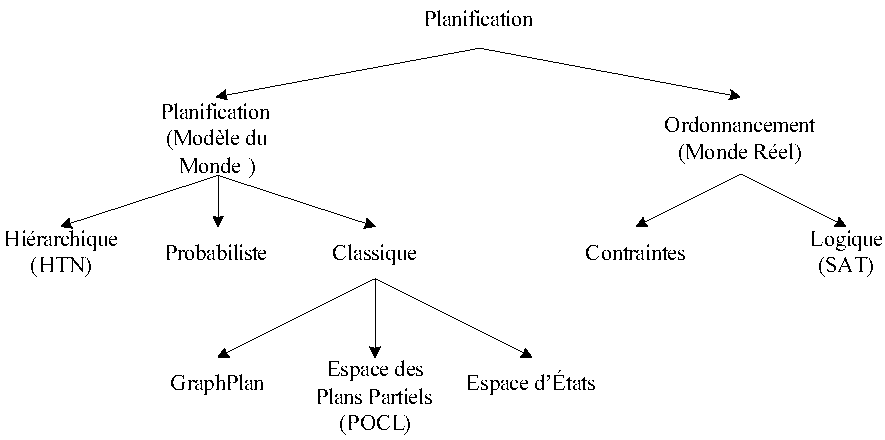
\includegraphics[width=.95\textwidth]{taxinomie}
    \caption{\label{fig:tax} Taxinomie de la planification inspir�e de~\cite{SFJ.00}.}
\end{center}
\end{figure}

Dans cette annexe, nous allons �tudier les diff�rentes m�thodes propos�es par les articles de~\cite{ZG.00} et de~\cite{DMRSW.03} au travers de la taxinomie pr�sent�e par~\cite{SFJ.00} (figure \ref{fig:tax}). Nous allons donc pr�senter dans un premier temps les m�thodes de planification d�crites dans~\citep{SFJ.00} et discuter de leur capacit� � g�rer le temps et les ressources, puis, dans un second temps nous positionnerons les strat�gies employ�es par~\cite{ZG.00}, \cite{DMRSW.03} ainsi que celle propos�e par~\cite{SFJ.00}.

\section{Planification classique}\label{strips}
La plupart des travaux en planification des trente derni�res ann�es se positionnent essentiellement dans le cadre la planification classique. Dans un probl�me de planification classique, l'objectif est d'atteindre un ensemble donn� de buts, usuellement repr�sent�s par des litt�raux (positifs ou n�gatifs) de la logique propositionnelle. L'�tat initial du monde est, quant � lui, �galement repr�sent� par des litt�raux. La planification consiste alors � trouver une succession d'actions possibles faisant �voluer le monde d'un �tat initial � un �tat but. Le langage de repr�sentation du monde g�n�ralement utilis� en planification classique est le langage \textsc{strips}\footnote{Pour STanford Research Institute Problem Solver} bas� sur les hypoth�ses restrictives suivantes:
\begin{itemize}
    \item l'agent est omniscient, au sens ou l'environnement est totalement observable\,; toute information est disponible et certaine � tout instant.
    \item les actions sont atomiques et d�terministes: aucune action de l'agent ne peut �tre interrompue et les effets des actions sont connus avec certitude.
    \item l'univers est statique, au sens ou si l'agent n'agit pas, l'environnement n'�volue pas.
\end{itemize}
Ces hypoth�ses peuvent g�n�ralement �tre �tendues pour permettre:
\begin{itemize}
    \item la prise en compte du temps (synchronisation d'actions, dur�e des actions, \dots),
    \item la prise en compte des ressources (�nergie, materiel, \dots),
    \item la prise en compte de l'incertitude (dynamique de l'environnement, incertitudes sur les effets des actions ou sur des �tats de l'environnement,~\dots).
\end{itemize}

Sous les hypoth�ses restrictives nous pouvons d�finir:
\begin{description}
\item[L'�tat:] Tout d'abord un �tat $e$ du monde de la planification est repr�sent� par un ensemble fini de formules atomiques sans symbole de variable. Une formule atomique de base est aussi appel�e un \emph{fluent}.
\item[L'action:] Ensuite, un op�rateur $o$ repr�sente un mod�le d'action. Un tel op�rateur est g�n�ralement d�fini par son nom et un triplet $<Prec, Add, Del>$ o� $Prec$, $Add$ et $Del$ sont des ensembles finis de fluents. $Prec(o)$ repr�sente les pr�conditions de l'op�rateur $o$, i.e. un ensemble fini de fluents qui doivent �tre v�rifi�s pour que l'op�rateur puisse �tre appliqu�. $Add(o)$ repr�sente les ajouts de $o$ i.e. un ensemble fini de fluents qui sont ajout�s � l'�tat du monde. Finalement, $Del(o)$ repr�sente les retraits de $o$, i.e. un ensemble fini de fluents qui sont retir�s de l'�tat du monde. Une action, d�not�e par $a$, est une instance de base d'un op�rateur $o$ (toutes les variables de $o$ sont instanci�es).
\end{description}

Dans ce contexte, un probl�me de planification est un triplet $<O, I, B>$ o�:
\begin{itemize}
\item $O$ d�note un ensemble fini d'op�rateurs utilisables dans le domaine de la planification consid�r�,
\item $I$ est l'�tat initial du probl�me, il est repr�sent� par un ensemble fini de fluents,
\item $B$ est le but du probl�me, il est repr�sent� par un ensemble fini de fluents.
\end{itemize}

Par exemple, dans le monde des blocs constitu� de deux blocs $B1$ et $B2$, un op�rateur pourrait �tre $Saisir(x)$. Les actions seraient alors instanci�es en $Saisir(B1)$ et $Saisir(B2)$.

Il existe dans la litt�rature un grand nombre de m�thodes et techniques qui se sont concentr�es sur la r�solution de probl�mes de planification classique. Notre objectif ici n'est pas de toutes les expliciter en d�tail, mais de couvrir les approches les plus r�pandues en se concentrant sur les id�es principales, les avantages et les d�fauts de chacune d'entre elles.

\subsection{Espaces d'�tats}

La recherche dans les espaces d'�tats consiste � explorer l'ensemble des �tats du monde atteignables par les actions disponibles pour trouver un �tat o� tous les buts sont v�rifi�s. Cette recherche correspond en fait � l'exploration d'un arbre ou les n\oe uds sont les �tats du monde et les arcs les actions appliqu�es pour passer d'un �tat � un autre (i.e les op�rateurs instanci�s). La recherche dans cet arbre peut se faire de deux mani�res: soit en partant de l'�tat initial du monde et en appliquant successivement les actions possibles jusqu'a atteindre un �tat but, soit en r�gressant un �tat but jusqu'a atteindre l'�tat initial:
\begin{itemize}
\item Application d'une action $a$ � un �tat $e$: $e \uparrow a$ (cha�nage avant) (cf. algorithme~\ref{Alg:fss}):
    \begin{itemize}
     \item une action $a$ est applicable sur un �tat $e$ ssi $Prec(a) \subseteq e$,
     \item le nouvel �tat est l'ensemble de fluents:\\
        $e \uparrow a = (e - Del(a)) \cup add(a)$
    \end{itemize}
\item R�gression d'un �tat $e$ par une action $a$: $e \downarrow a$ (cha�nage arri�re) (cf. algorithme~ \ref{Alg:goa}):
    \begin{itemize}
     \item la r�gression d'un �tat (partiel) $b$ � travers une action $a$ est possible ssi:
        \begin{itemize}
         \item $a$ est une action pertinente: $add(a) \cap b \neq \emptyset$ et
         \item $a$ est une action consistante avec $b$ : $Del(a) \cap b = \emptyset$,
        \end{itemize}
     \item le nouvel �tat (partiel) est l'ensemble de fluents:\\
     $b \downarrow a = (b - add(a)) \cup Prec(a)$
    \end{itemize}
\end{itemize}

Ce type de recherche engendre un tr�s grand nombre d'�tats � explorer pour trouver un �tat satisfaisant les buts. Il existe cependant un bon nombre d'algorithmes des plus na�fs (profondeur d'abord, largeur d'abord, \dots) aux plus efficaces (A, A$^\star$, WA$^\star$, A$^\star\star$ \dots), ces derniers n�cessitant des heuristiques plus ou moins complexes souvent bas�es sur la connaissance du domaine du probl�me, mais permettant de guider la recherche. Les planificateurs utilisant ce type d'algorithmes de recherche avec heuristique sont � ce jour les plus performants en terme de vitesse pour trouver une solution en comparaison des algorithmes d�crits un peu plus loin, bien que les plans solution trouv�s soient souvent plus co�teux que ceux g�n�r�s par les autres algorithmes.

Un des probl�mes majeurs de la recherche dans les espaces d`�tats est qu'elle ne permet de trouver que des plans s�quentiels, totalement ordonn�s, n'autorisant pas la parall�lisation d'actions ind�pendantes\footnote{Une d�finition de l'ind�pendance de deux actions peut �tre trouv�e dans la section \ref{interactions}} et ne profitant pas de la d�composition du probl�me.

\begin{algorithm}
\caption{$ChainageAvant(EtatCourant,PlanSolution)$. \label{Alg:fss}}
\begin{algorithmic}[1]
    \If{$buts \subseteq EtatCourant$}
        \State{\Return($PlanSolution$)}
    \EndIf
    \State{\textbf{Choisir} une action $A$ (instance d'un op�rateur) t.q.:}
    \Statex{\hspace{1cm} $Prec(A)\subseteq EtatCourant$}
    \Statex{\hspace{1cm} et suivant une heuristique}
    \If{$A$ n'existe pas}
        \State{\textbf{�chec}}
    \EndIf
    \State{Construire un nouvel �tat $EtatSuivant$:}
    \Statex{\hspace{1cm} $EtatSuivant \leftarrow (EtatCourant \setminus Del(A)) \cup Add(A)$}
    \State $ChainageAvant(EtatSuivant,PlanSolution \mid A)$
\end{algorithmic}
%\caption{ Algorithme de recherche dans les espaces d'�tats par cha�nage avant. Le choix de l'action est un point de backtrack.}
\end{algorithm}

\begin{algorithm}
\caption{$ChainageArriere(Buts,Contraintes,PlanSolution)$. \label{Alg:goa}}
\begin{algorithmic}[1]
    \If{$\square \models Contraintes$}\Comment{Si on ne peut satisfaire les contraintes}
        \State{\textbf{�chec}}
    \EndIf
    \If{$Buts \subseteq EtatInitial$}
        \State{\Return($PlanSolution$)}
    \EndIf
    \State{S�lectionner un but $b \in Buts$}
    \State{\textbf{Choisir} une action $A$ (instance d'un op�rateur) t.q.:}
    \Statex{\hspace{1cm} $b \in Add(A)$}
    \Statex{\hspace{1cm} et suivant une heuristique}
    \If{$A \in PlanSolution$}
        \State{$ChainageArriere(Buts \setminus \{b\},$ $ContraintesMAJ,$\,$PlanSolution)$}
    \Else{$ChainageArriere((Buts \cup Prec(A))\setminus\,\{b\}, ContraintesMAJ, PlanSolution \mid A)$}
    \EndIf
\end{algorithmic}
%\caption{Algorithme de recherche dans les espaces d'�tats par cha�nage avant. Le choix de l'action est un point de backtrack.}
\end{algorithm}

\subsection{Espace des Plans Partiels}\label{sect:epp}

La recherche dans l'espace des plans partiels a �t� popularis�e par~\cite{MAR.91}. Elle se base sur une recherche par cha�nage arri�re vue dans la section pr�c�dente: L'id�e est de choisir une action qui puisse �tablir un des buts et de l'ajouter au plan. Le but est alors retir� de l'ensemble de buts � atteindre et remplac� par des sous-buts correspondant aux pr�conditions de l'action. Ce processus est r�p�t� jusqu'a ce que tous les sous-buts restants soit une sous-partie de l'ensemble des conditions initiales. Ainsi, cette approche permet de travailler sur plusieurs sous-buts ind�pendamment, de les r�soudre � l'aide de plusieurs sous-plans puis de combiner ces sous-plans.

Un plan partiel est d�fini comme un triplet $<OP, CO, CI>$ o�:
\begin{itemize}
\item $OP$ est l'ensemble des op�rateurs du plan partiel,
\item $CO$ est un ordre partiel sur OP, autrement dit, c'est l'ensemble des contraintes de pr�c�dence qui lient les op�rateurs deux � deux,
\item $CI$ est l'ensemble des contraintes d'instanciation des variables associ�es au plan.
\end{itemize}

L'espace de recherche est donc encore une fois un arbre o� les n\oe uds sont des plans partiels et ou les arcs sont les op�rations de modification de ces plans partiels:
\begin{itemize}
    \item \emph{Choix d'un �tablisseur}: On appelle une action $E$ un �tablisseur ssi $\exists A$, $Add(E) \cap Prec(A) \neq \emptyset$. � partir de l�, choisir un �tablisseur, c'est placer avant une action $A$ une autre action $E$ pour �tablir une pr�condition de $A$\,;
    \item \emph{Promotion d'un casseur}: On appelle une action $C$ un casseur ssi $\exists E$, $Del(C) \cap Add(E) \neq \emptyset$. Promouvoir un casseur $C$, c'est le contraindre � s'ex�cuter avant l'�tablisseur $E$: $C \prec E \prec A$ (l'�tablissement de la pr�condition de $A$ par $E$ n'est pas remis en cause par $C$)\,;
    \item \emph{S�paration casseur/demandeur} : On appelle une action $A$ un demandeur ssi un fluent des pr�conditions de $A$ n'a pas encore �t� �tabli. S�parer un casseur $C$ et un demandeur $A$, c'est contraindre l'instanciation de $C$ pour qu'il ne nuise pas � $A$ par la suite ($C$ ne peux emp�cher d'�tablir la pr�condition de $A$ qui est concern�e)\,;
    \item \emph{D�motion d'un casseur}: D�mettre un casseur $C$, c'est contraindre $C$ � s'ex�cuter apr�s $A$: $A \prec C$ ($C$ ne d�truira pas la pr�condition de $A$ cr��e par $E$)\,;
    \item \emph{Choix d'un white knight}: Choisir un white knight $W$, c'est placer entre $C$ et $A$ une action $W$ pour r�tablir les pr�conditions de $A$ d�truites par $C$. $W$ n'a g�n�ralement pas de pr�conditions ni de retraits ($Prec(W) = \emptyset$ et $Del(W) = \emptyset$ ).
\end{itemize}

� l'aide de ces op�rations sur les plans partiels, il devient ais� de construire un plan en instanciant les op�rateurs de $OP$. Chaque instanciation d'op�rateur est ajout�e � l'ensemble $CI$. Les contraintes de pr�c�dence, que ce soit pour les choix d'�tablisseurs ou la promotion/d�motion de casseurs sont ajout�s au cours de la r�solution dans l'ensemble $CO$. Des exemples de planification dans les espaces de plans partiels peuvent �tre trouv�s dans~\citep{RN.03} pp. 391--393.

\subsection{Graphplan}\label{sect:graphplan}
Graphplan est un algorithme � part des deux autres approches vues pr�c�demment. Il se base sur un graphe de planification. Ce graphe de planification permet, en plus d'extraire un plan � l'aide de Graphplan, de fournir des informations utiles � la cr�ation d'heuristiques efficaces pour les algorithmes d�crits auparavant.

Un graphe de planification est, selon~\cite{RN.03}, une s�quence de niveaux correspondant aux �tapes de temps dans le plan, o� le niveau z�ro est l'�tat initial. Chaque niveau contient un ensemble de fluents et un ensemble d'actions (des instances des op�rateurs). Les fluents sont ceux qui sont \emph{possiblement} pr�sents � cette �tape du plan, les actions, celles qui ont leurs pr�conditions \emph{possiblement} satisfaites � cette �tape du plan. Il peut n�anmoins arriver que des interactions n�gatives apparaissent entre les actions les emp�chant de s'ex�cuter simultan�ment. \label{interactions}On d�finit les interactions de la mani�re suivante:

\begin{definition}
Interactions \emph{positives}: Deux actions a1, a2 sont en interaction positive ssi:
\begin{itemize}
    \item $Add/Add: \exists f, f \in Add(a1) \cap Add(a2)$
    \item $Add/Prec: \exists f, f \in Add(a1) \cap Prec(a2)$
\end{itemize}
\end{definition}

\begin{definition}
Interactions \emph{n�gatives}: Deux actions a1, a2 sont en interaction n�gative ssi:
\begin{itemize}
    \item Effets antagonistes: $\exists f, f \in Add(a1) \cap Del(a2)$ ou
    \item Interactions crois�es: $\exists f, f \in Del(a2) \cap Prec(a1)$
\end{itemize}
\end{definition}

\begin{definition}
Interactions \emph{ind�pendantes}: Deux actions a1, a2 sont ind�pendantes (not� a1 \# a2) ssi elles n'ont pas d'interactions n�gatives i.e.,
\begin{itemize}
    \item $Del(a1) \cap (Prec(a2) \cup Add(a2)) = \emptyset$ et
    \item $Del(a2) \cap (Prec(a1) \cup Add(a1)) = \emptyset$
\end{itemize}
\end{definition}

De la, on peut d�finir des fluents et des actions mutuellement exclusives:
\begin{definition}
Actions \emph{mutuellement exclusives}: Deux actions d'un m�me niveau dans le graphe de planification sont mutuellement exclusives (\emph{mutex}) ssi:
\begin{itemize}
    \item elles ne sont pas ind�pendantes ou,
    \item elles ont des pr�conditions \emph{mutex} au niveau pr�c�dent (elles ne peuvent donc pas �tre d�clench�es en m�me temps) (voir D�finition \ref{mutex}):\\
$ \exists (p,q) \in Prec(a1) \times Prec(a2)$, telles que p et q sont \emph{mutex}.
\end{itemize}
\end{definition}

\begin{definition}\label{mutex}
Fluents \emph{mutuellement exclusifs}: Deux fluents p et q sont \emph{mutex} au niveau i ssi tous les couples d'actions qui les produisent � ce m�me niveau sont \emph{mutex}:
$\forall a1, a2$ t.q.  $p \in Add(a1)$, $q \in Add(a2),$ a1 et a2 \emph{mutex}.
\end{definition}

\begin{figure}[!hbt]
\begin{center}
    %\includegraphics[width=0.9\textwidth]{graphplan}
    \begin{tikzpicture}
   [  yscale=0.7, xscale=1.3, scale=1.6,
      pre/.style={<-,shorten <=0pt,>=stealth},
      post/.style={->,shorten >=0pt,>=stealth},
      actionMutex/.style={thick,color=blue!90!green,bend left=#1,thin,densely dashed},
      fluentMutex/.style={thick,color=green!90!blue,bend left=#1},
      maintienFluent/.style={very thick,color=red},
      ajoutFluent/.style={thick,color=black},
      retraitFluent/.style={very thick,densely dashed,color=black},
      information text/.style={draw, thick, rounded corners,inner sep=1ex}]

% =========================================================================
% =============================== LE SCHEMA ===============================
% =========================================================================

       \node (n0)      at (0,0)            {$a$};

      \node (n11)     at (1,1.5)          {$A$}
         edge [pre,ajoutFluent]        (n0);
      \node (n10)     at (1,0)            {$N_a$}
         edge [pre,maintienFluent]    (n0);
      \node (n1-1)    at (1,-1.5)         {$B$}
         edge [pre,ajoutFluent]        (n0)
         edge [actionMutex=-10]         (n10)
         edge [actionMutex=10]         (n11);
      \node          at (0,-4)            {Niveau 0};

      \node (n21)     at (2,3)            {$b$}
         edge [pre,ajoutFluent]        (n11);
      \node (n20)     at (2,0)            {$a$}
         edge [pre,maintienFluent]    (n10)
         edge [pre,retraitFluent]      (n1-1);
      \node (n2-1)    at (2,-3)           {$c$}
         edge [pre,ajoutFluent]        (n1-1)
         edge [fluentMutex=10]         (n21)
         edge [fluentMutex=0]         (n20) ;
      \node          at (2,-4)            {Niveau 1};

      \node (n32)    at (3,3)             {$N_b$}
         edge [pre,maintienFluent]    (n21);
      \node (n31)    at (3,1.5)           {$A$}
         edge [pre,ajoutFluent]        (n20);
      \node (n30)    at (3,0)             {$N_a$}
         edge [pre,maintienFluent]    (n20);
      \node (n3-1)    at (3,-1.5)         {$B$}
         edge [pre,ajoutFluent]        (n20)
         edge [actionMutex=0]          (n30)
         edge [actionMutex=-10]         (n31);
      \node (n3-2)    at (3,-3)           {$N_c$}
         edge [actionMutex=0]          (n3-1)
         edge [actionMutex=-10]         (n30)
         edge [actionMutex=10]         (n31)
         edge [actionMutex=10]         (n32)
         edge [pre,maintienFluent]    (n2-1);

      \node (n41)     at (4,3)            {$b$}
         edge [pre,maintienFluent]    (n32)
         edge [pre,ajoutFluent]        (n31);
      \node (n40)     at (4,0)            {$a$}
         edge [pre,maintienFluent]    (n30)
         edge [pre,retraitFluent]      (n3-1);
      \node (n4-1)    at (4,-3)           {$c$}
         edge [pre,ajoutFluent]        (n3-1)
         edge [fluentMutex=0]            (n40)
         edge [pre,maintienFluent]    (n3-2);
      \node          at (4,-4)            {Niveau 2};

      \node (n53)    at (5,3)             {$N_b$}
         edge [pre,maintienFluent]    (n41);
      \node (n52)    at (5,2)             {$A$}
         edge [pre,ajoutFluent]        (n40);
      \node (n51)    at (5,1)             {$C$}
         edge [pre,ajoutFluent]        (n41)
         edge [pre,ajoutFluent]        (n4-1)
         edge [actionMutex=0]          (n52);
      \node (n50)    at (5,0)             {$N_a$}
         edge [actionMutex=0]          (n51)
         edge [pre,maintienFluent]    (n40);
      \node (n5-1)    at (5,-1.5)         {$B$}
         edge [pre,ajoutFluent]        (n40)
         edge [actionMutex=0]          (n50)
         edge [actionMutex=-10]         (n51)
         edge [actionMutex=10]          (n52);
      \node (n5-2)    at (5,-3)           {$N_c$}
         edge [actionMutex=0]          (n5-1)
         edge [actionMutex=-10]         (n50)
         edge [pre,maintienFluent]     (n4-1)
         edge [actionMutex=10]          (n52);

      \node (n62)     at (6,3)            {$b$}
         edge [pre,maintienFluent]    (n53)
         edge [pre,ajoutFluent]        (n52);
      \node (n61)     at (6,1.5)    [rectangle,draw=blue!50,rounded corners=1pt,thick, fill=blue!10]      {$d$}
         edge [pre,ajoutFluent]        (n51);
      \node (n60)     at (6,0)            {$a$}
         edge [pre,maintienFluent]    (n50)
         edge [pre,retraitFluent]      (n5-1);
      \node (n6-1)    at (6,-3)           {$c$}
         edge [pre,ajoutFluent]        (n5-1)
         edge [fluentMutex=10]          (n61)
         edge [pre,maintienFluent]    (n5-2);
      \node          at (6,-4)            {Niveau 3};

% ==========================================================================
% =============================== LA LEGENDE ===============================
% ==========================================================================

      \node [below right] (acMut) at  (0.1, -5)         {Actions Mutex};
      \node (acMutEmpty)      [left=of acMut]    {}
         edge [actionMutex=0]    (acMut);
      \node [below right] (fluMut) at (0.1, -5.6)     {Fluents Mutex};
      \node (fluMutEmpty)     [left=of fluMut]   {}
         edge [fluentMutex=0] (fluMut);
      \node [below right] (maintFlu) at (0.1, -6.2)     {Maintien de fluent};
      \node (maintFluEmpty) [left=of maintFlu] {}
         edge [post,maintienFluent] (maintFlu);
      \node [below right] (ajoutFlu) at (0.1, -6.8)     {Ajout de fluent};
      \node (ajoutFluEmpty) [left=of ajoutFlu] {}
         edge [post,ajoutFluent] (ajoutFlu);
      \node [below right] (retraitFlu) at (0.1, -7.4)   {Retrait de fluent};
      \node (retraitFluEmpty) [left=of retraitFlu] {}
         edge [post,retraitFluent] (retraitFlu);

% =========================================================================
% ============================== LES ACTIONS ==============================
% =========================================================================

\draw[]
   node[below right, text width=6cm, information text] at (2.7,-5)
   {
      \begin{center}
         {\bf Actions}
      \end{center}
      \vspace{-.6cm}
      \begin{multicols}{2}
      $A$ : $a \rightarrow +b$ \\
      $B$ : $a \rightarrow +c-a$ \\
      $C$ : $bc \rightarrow +d$ \\~\\
      $N_a$ : $a \rightarrow +a$ \\
      $N_b$ : $b \rightarrow +b$ \\
      $N_c$ : $c \rightarrow +c$ \\
      $N_d$ : $d \rightarrow +d$
      \end{multicols}

   };
\end{tikzpicture}


    \caption{\label{afig:graphplan} Un exemple de graphe de planification.}
\end{center}
\end{figure}

Graphplan poss�de plusieurs propri�t�s importantes: En dehors de la possibilit� de rechercher directement un plan � l'int�rieur avec Graphplan, il fournit suffisamment d'informations qui permettent de produire des heuristiques tr�s efficaces pour la recherche dans les espaces d'�tats ou de plans partiels.  De plus il se construit de mani�re polyn�miale en temps et en espace par rapport � la taille des donn�es (le nombre d'actions possibles dans le plan), une propri�t� tr�s int�ressante dans ce domaine. Le probl�me est que la recherche d'un plan solution dans ce graphe de planification est, elle, exponentielle.

Un exemple de graphe de planification est fourni par la figure \ref{afig:graphplan}. Le niveau 0 comprend les fluents existant � l'�tat initial. Au niveau 1 apparaissent les actions pouvant �tre ex�cut�es ainsi que les ajouts et retraits qu'elles effectuent. D�s lors, on voit appara�tre � ce niveau des actions \emph{mutex} dues au fait que l'action $B$ retire le fluent $a$ de l'environnement, n�cessaire � l'ex�cution de l'action $A$ et � l'action $N\_a$ (action qui consiste juste � simuler que $a$ n'a pas disparu entre deux niveaux). Par cons�quent, le fluent $c$ ajout� par $B$ au niveau 1 se retrouve \emph{mutex} avec les ajouts de $A$ et $N\_a$ (resp. les fluents $b$ et $a$). Ensuite, au niveau 2, toutes les actions ayant des pr�conditions \emph{mutex}, se retrouvent �galement \emph{mutex}. Et ainsi de suite jusqu'a ce qu'apparaisse le fluent $d$ (notre but, encadr� figure \ref{afig:graphplan}) au niveau 4. Le fluent $d$ n'a pas pu �tre obtenu avant car l'action $C$ qui l'ajoute au monde poss�de comme pr�condition les fluents $b$ et $c$ qui �taient \emph{mutex} jusqu'au niveau 3. Enfin, � l'aide de l'algorithme Graphplan (Algorithme non donn� ici mais bas� sur un cha�nage arri�re donn� par l'algorithme \ref{Alg:goa}), on peut extraire un plan de ce graphe de planification comme indiqu� en gras/encadr� dans la figure~\ref{afig:graphplan2}.

\begin{figure}[!hbt]
\begin{center}
    %\includegraphics[width=0.8\textwidth]{graphplan2}
    \begin{tikzpicture}
   [  yscale=0.7, xscale=1.3, scale=1.6,
      pre/.style={<-,shorten <=0pt,>=stealth},
      post/.style={->,shorten >=0pt,>=stealth},
      base/.style={draw, very thick,color=red},
      maintienFluent/.style={base},
      ajoutFluent/.style={base},
      texty/.style={base, rounded corners,inner sep=1ex}]
% =========================================================================
% =============================== LE SCHEMA ===============================
% =========================================================================

\begin{scope}
    \tikzstyle{every node}=[texty] %%
     \node (n0)      at (0,0)            {$a$};

      \node (n11)     at (1,1.5)          {$A$}
         edge [pre,ajoutFluent]        (n0);
      \node (n10)     at (1,0)            {$N_a$}
         edge [pre,maintienFluent]    (n0);

      \node (n21)     at (2,3)            {$b$}
         edge [pre,ajoutFluent]        (n11);
      \node (n20)     at (2,0)            {$a$}
         edge [pre,maintienFluent]    (n10);

      \node (n32)    at (3,3)             {$N_b$}
         edge [pre,maintienFluent]    (n21);
      \node (n3-1)    at (3,-1.5)         {$B$}
         edge [pre,ajoutFluent]        (n20);

      \node (n41)     at (4,3)            {$b$}
         edge [pre,maintienFluent]    (n32);
       \node (n4-1)    at (4,-3)           {$c$}
         edge [pre,ajoutFluent]        (n3-1);

      \node (n51)    at (5,1)             {$C$}
         edge [pre,ajoutFluent]        (n41)
         edge [pre,ajoutFluent]        (n4-1);

      \node (n61)     at (6,1.5)          {$d$}
         edge [pre,ajoutFluent]        (n51);
\end{scope}

      \node          at (0,-4)            {Niveau 0};
      \node          at (2,-4)            {Niveau 1};
      \node          at (4,-4)            {Niveau 2};
      \node          at (6,-4)            {Niveau 3};

\end{tikzpicture}


    \caption{\label{afig:graphplan2} Extraction de plan d'un graphe de planification.}
\end{center}
\end{figure}

\subsection{Discussion}
\label{dis:STRIPS}
Malgr� leur efficacit�, les algorithmes classiques pr�c�demment �voqu�s, utilisables dans des environnements d�terministes et totalement observables, ont de s�rieuses limitations attribu�es � \textsc{strips}:
\begin{description}
    \item[Temps:] Il n'existe pas de repr�sentation explicite du temps dans la repr�sentation \textsc{strips}. Il n'est pas possible de sp�cifier la dur�e d'une action ou des contraintes de temps entre les buts ou les actions.
    \item[Ressources:] Rien n'est pr�vu dans la repr�sentation pour sp�cifier les besoins en ressources ou pour mod�liser la consommation de ressources.
    \item[Incertitude:] \textsc{strips} n'a pas la capacit� de mod�liser l'incertitude. L'�tat initial doit �tre connu enti�rement et les buts, une fois atteints, sont consid�r�s comme certains.\\
\end{description}

N�anmoins, de nombreuses extensions de \textsc{strips} existent. Tant pour la mod�lisation du temps~\citep{SW.99,PW.94} que pour la gestion de nombreux types de ressources~\citep{KW.99,K.98} ou de l'incertitude~\citep{WAS.98,DHW.94}. Seulement, ce type d'extensions d�g�n�rent significativement les performances~\citep{SFJ.00}.

Ceci dit, si l'on ne consid�re que les m�thodes intrins�quement, depuis le syst�me TWEAK de~\cite{Ch.87} et jusqu'aux formalisations de~\cite{KS.96}, l'approche de la planification �tait essentiellement fond�e sur les strat�gies de raffinements dans les espaces de plans partiels, les autres approches �tant tr�s marginalis�es au sein de la communaut�.

En 1995 cependant, l'apparition du planificateur Graphplan fut � l'origine d'un bouleversement de cet ordre bien �tabli. Les id�es qui guidaient sa conception ont initi� des travaux qui ont permis aux algorithmes de planification d'augmenter leurs performances de mani�re si importante que l'on peut maintenant commencer � envisager des applications r�elles. Par un curieux retour des choses, la planification par recherche heuristique dans les espaces d'�tats s'est (re)trouv�e �tre tr�s performante avec l'apparition de planificateurs utilisant des heuristiques inspir�es par Graphplan. Elle permet actuellement de r�soudre des probl�mes qui �taient tr�s largement hors de port�e des planificateurs il y a seulement quelques ann�es, mais toujours dans le cadre des limitations de \textsc{strips}.

Plusieurs m�thodes algorithmiques, issues d'autres domaines classiques de l'IA sont maintenant en concurrence : recherche heuristique dans les espaces d'�tats, dans les espaces de plans partiels, Graphplan, planification \textsc{sat}, planification \textsc{csp}, recherche locale, etc. Les diff�rents planificateurs qui en d�coulent font l'objet d'�valuations comparatives r�guli�res dans le cadre des comp�titions IPC (\emph{International Planning Competition}) des conf�rences AIPS, et maintenant ICAPS.

Il est � noter que nous avons d�lib�r�ment omis de citer les m�thodes de planification \textsc{sat} pour la simple mais excellente raison que la repr�sentation de contraintes temporelles en logique propositionnelle augmente consid�rablement le nombre de clauses \textsc{sat} et rend la r�solution proprement impossible. Il en est tout de m�me fait �tat dans~\citep{SFJ.00} car ce type de mod�lisation permet ais�ment la repr�sentation des ressources et l'optimisation. Dans un contexte d'utilisation de la planification sur des horizons infinis ou en temps continu, nous ne pouvons pas prendre en compte une approche complexifiant � ce point la repr�sentation du temps.

\section{Planification hi�rarchique}

La plupart des planificateurs d�velopp�s dans le cadre d'applications r�elles utilisent les r�seaux de hi�rarchisation de t�ches (\textsc{htn} pour \emph{Hierarchical Task Network}). La principale diff�rence avec la planification classique et est que cette derni�re essaie de d�composer des t�ches de haut niveau en t�ches de plus bas niveau l� o� la planification classique cherche juste � assembler des actions pour atteindre des buts. De plus, un but est plut�t sp�cifi�, dans la planification hi�rarchique, comme une t�che de haut niveau, que comme un ensemble de litt�raux � obtenir.

L'algorithme de planification consiste donc � d�composer chaque t�che en t�ches �l�mentaires, tout en v�rifiant qu'elles n'aient pas d'interactions n�gatives entre elles. La planification se termine lorsque le r�seau ne contient que des t�ches �l�mentaires et lorsque l'ensemble des contraintes d'ordre relatives � la gestion des conflits est consistant (i.e. qu'il n'existe pas de boucles). L'algorithme \ref{Alg:htn} est une simplification en pseudo-code de la planification hi�rarchique.

\begin{algorithm}
\caption{\label{Alg:htn} $\textsc{htn}-Plan(Plan)$}
\begin{algorithmic}[1]
    \If{$Plan$ contient des conflits}
        \If{il n'existe pas de mani�re de r�soudre les conflits}
            \State{\textbf{�chec}}
        \Else{\textbf{Choisir} une mani�re de r�soudre les conflits et l'appliquer}
        \EndIf
    \EndIf
    \If{$Plan$ ne contient que des t�ches �l�mentaires}
        \State{\Return($Plan$)}
    \EndIf
    \State{S�lectionner une t�che non �l�mentaire $t \in Plan$}
    \State{\textbf{Choisir} une d�composition $E$ de $t$}
    \State{$NouveauPlan \leftarrow$ Remplacer $t$ par $E$ dans $Plan$}
    \State{$\textsc{htn}-Plan(NouveauPlan)$}
\end{algorithmic}
\end{algorithm}

Le temps et la gestion de donn�es m�triques ne posent pas de r�elles difficult�s pour les planificateurs \textsc{htn}. Ces contraintes peuvent �tre directement sp�cifi�e � l'int�rieur des t�ches ou alors �valu�es pas le biais de test de consistance de l'algorithme. Seulement, selon~\cite{SFJ.00}, les planificateurs \textsc{htn} essuient pour le moment trois critiques importantes:
\begin{description}
    \item[S�mantique:] Il n'existe pas de s�mantique bien d�finie pour la d�composition de t�che, cela a pour cons�quence de rendre difficile tout jugement de la compl�tude ou de la consistance d'un plan.
    \item[Conception:] La conception de ce type de planificateur n�cessite de pr�voir et d'analyser toutes les t�ches possiblement existantes et d�composables. Il est vraiment difficile d'une part, de produire la liste exhaustive de toutes les d�compositions d'une t�che, mais d'autre part, � chaque ajout de fonctionnalit� au syst�me, il faudra pr�voir et lister toutes les nouvelles d�compositions � ajouter pour utiliser au mieux les fonctionnalit�s du syst�me.
    \item[Fragilit�:] Les planificateurs \textsc{htn} sont loins d'�tre robustes. En effet, ils sont incapables de prendre en compte des t�ches non explicitement pr�vues par le concepteur, m�me si les t�ches �l�mentaires sont suffisantes pour construire un plan correct.
\end{description}

\section{Planifications probabilistes}

Jusqu'� pr�sent nous avons consid�r� que des domaines de la planification classique totalement observables, statiques et d�terministes. De plus nous avons consid�r� que la description des actions �tait correcte et compl�te. Dans ces circonstances, un agent peut, apr�s avoir �labor� un plan, l'ex�cuter sans aucune surprise d'aucunes sorte. En revanche, dans un environnement incertain, cet agent devra utiliser ses moyens de perception pour analyser et �ventuellement anticiper en modifiant ou en adaptant son plan en cours d'ex�cution. Les m�thodes utilis�es pour r�agir dans ces types d'environnements utilisant les probabilit�s d'occurrence d'�v�nements incertains pour les pr�voir et les mod�liser, sont qualifi�es de probabilistes. Une autre classe de m�thodes utilisant la logique pour mod�liser l'incertitude ne sera pas �tudi�e ici puisqu'elle n'intervient pas dans la cat�gorisation des techniques int�ressantes pour notre th�se.

Il existe selon~\cite{RN.03} quatre m�thodes de planification probabilistes, les deux premi�res sont plus attach�es � r�soudre les probl�mes � ind�termination limit�e (dans le sens o� les actions ont un nombre fixe d'effets d�finis ayant chacun sa probabilit� d'occurrence), les deux suivantes s'attachent plus � l'ind�termination pure (dans le sens ou les actions ont des effets en trop grand nombre ou inconnus):
\begin{itemize}
    \item \emph{Planification Aveugle}: Aussi connue sous le nom de planification \emph{conformante}, cette m�thode construit un plan standard s�quentiel qui doit pouvoir �tre ex�cut� sans perceptions. Le plan construit doit pouvoir assurer d'atteindre les buts voulus dans toutes les circonstances possibles en regard des certitudes sur l'�tat initial et des sorties actuelles des actions.
    \item \emph{Planification Conditionnelle}: Aussi connue sous le nom de planification contingente, cette approche ajoute des branches conditionnelles au plan aux endroits ou pourraient survenir des contingences. L'agent choisit quelle branche du plan ex�cuter en utilisant ses percepts comme test conditionnel.
    \item \emph{Supervision d'ex�cution et replanification }: Dans cette approche, un agent peut utiliser toutes les techniques vues pr�c�demment (classique, aveugle ou contingente) pour produire un plan, mais ajoute � cela une supervision de l'ex�cution. La replanification intervient lorsque l'ex�cution ne se passe pas comme pr�vu.
    \item \emph{Planification continue}: Tous les planificateurs vus ci-dessus cont con�us pour atteindre un but et s'arr�ter. Un planificateur continu est con�u pour durer ind�finiment. Il est capable de supporter les impr�vus et m�me jusqu'a l'abandon des buts courants en utilisant des m�canismes de reformulation des buts.\\
\end{itemize}
Il existe �galement toute la planification sous incertain repr�sent�e essentiellement par les mod�les de Markov et d�taill�e au chapitre~\ref{chap:2} que nous ne pr�senterons donc pas ici. 
\newpage\phantom{a}
%\chapter{Th�orie de l'Information appliqu�e aux \pac{pomdp}s}
\label{anx:it}

\begin{summary}
Dans cette annexe les concepts de th�orie de l'information telle que l'entropie ou l'information mutuelle sont introduits pour ensuite les appliquer dans le contexte des \pomdps. Un r�sultat th�orique est d�riv� montrant que l'entropie ne peut converger si le taux d'entropie instantan� de la cha�ne de Markov sous-jacente au \pomdp et � la politique n'est pas born� sup�rieurement. Plusieurs exp�rimentations ont �galement �t� r�alis�es et sont rapport�es � la fin de cette annexe.
\end{summary}

\section{Entropie d'un �tat de croyance}

Une mesure couramment utilis�e en th�orie de l'information de la quantit� d'information et de la qualit� de l'information contenue dans un distribution de probabilit� telle que l'estimation d'un �tat de croyance~\citep{FBT.98} est l'entropie de~\cite{S.48}. L'entropie mesure la quantit� d'incertitude contenue dans une distribution de probabilit� discr�te ou continue. Dans le cas particulier d'un �tat de croyance sur un ensemble fini d'�tat, l'entropie $H$ est calcul�e en utilisant la formule suivante:
\begin{equation}\label{aeq:entropy}
    H(\bel^t) = -\sum_{s\in\Sta} \bel^t(s) \log \bel^t(s)
\end{equation}
L'entropie est maximale est �gale � $\log|\Sta|$ lorsque l'�tat de croyance est uniforme -- i.e il est possible d'�tre dans tous les �tats de mani�re �quiprobable -- et tend vers zero � mesure que l'�tat de croyance devient d�terministe\footnote{Par convention, $0\log 0\equiv 0$.}.

Dans la litt�rature de la th�orie de l'information, l'entropie associ�e � l'estimation de l'�tat courant a rarement �t� �tudi�e, except� par~\cite{R.06} qui a appel� cette quantit� \emph{entropie d'estimation}. En fait, cette entropie d'estimation, que nous noterons  $H(\bel^t)$, est �gale � l'entropie de la distribution sur les �tats �tant donn�e une s�quence d'observations re�ues. Elle se calcule donc de la mani�re suivante:
\begin{equation}\label{aeq:EstimationEntropy}
    H(\bel^t) = H(s^t|o^t,o^{t-1},\dots,o^1) = H(s^t|o^t,\bel^{t-1})
\end{equation}

Ainsi en utilisant les r�gles connues de th�orie de l'information, il est possible d'�noncer la proposition suivante:
\begin{proposition}\label{ap:beliefEntropy} L'entropie $H(\bel^t)$ d'un �tat de croyance � l'�tape $t$ depuis un �tat de croyance $\bel^{t-1}$ �tant donn�e n'importe quelle politique est donn�e par l'�quation suivante:
\begin{equation}\label{aeq:beliefEntropyF}
H(\bel^t) = H(s^t) - I(s^t;\bel^{t-1}) - I(o^t;s^t|\bel^{t-1}) \qquad
\end{equation}
\end{proposition}
\begin{proof}\begin{eqnarray}
  H(\bel^t)  &=& H(o^t|s^t,\bel^{t-1}) - H(o^t|\bel^{t-1}) + H(s^t|\bel^{t-1})\notag\\
             &=& - I(o^t;s^t|\bel^{t-1}) + H(s^t|\bel^{t-1})\notag\\
   \mbox{since }I(X;Y)  &=& H(X) - H(X|Y)\notag%\\
\end{eqnarray}
O� $H(s^t)$ est le \emph{taux instantan� d'entropie}~\citep{CT.91} de la cha�ne de Markov sous-jacente � la politique qui se construit par la combinaison de la politique et de la fonction de transition. $I(s^t;\bel^{t-1})$ est l'\emph{information mutuelle} entre l'�tat $s^t$ et l'�tat de croyance � l'�tape $t-1$ et $I(o^t;s^t|\bel^{t-1})$ l'\emph{information mutuelle conditionnelle} entre l'�tat $s^t$ et l'observation $o^t$ �tant donn�e l'�tat de croyance � l'�tape pr�c�dente.
\end{proof}

L'information mutuelle mesure l'ind�pendance mutuelle de deux variables al�atoires ou la quantit� d'information que deux variables al�atoires partagent. Elle est donn�e par:
\begin{eqnarray*}
I(X;Y) & = & \sum_{y \in Y} \sum_{x \in X} p(x,y) \log{ \left( \frac{p(x,y)}{p_1(x)\,p_2(y)} \right) }, \,\! \\
&  = & H(X) - H(X|Y) \\
&  = & H(Y) - H(Y|X) \\
&  = & H(X) + H(Y) - H(X,Y) \\
&  = & H(X,Y) - H(X|Y) - H(Y|X).
\end{eqnarray*}

L'information mutuelle conditionnelle mesure la m�me quantit� d'information, mais �tant donn�e une troisi�me variable al�atoire:
\[I(X;Y|Z) = \mathbb E_Z \big(I(X;Y)|Z\big)
    = \sum_{z\in Z} \sum_{y\in Y} \sum_{x\in X}
      p_Z(z) p_{X,Y|Z}(x,y|z) \log \frac{p_{X,Y|Z}(x,y|z)}{p_{X|Z}(x|z)p_{Y|Z}(y|z)},\]
Qui peut �tre simplifi�e en:
\[I(X;Y|Z) = \sum_{z\in Z} \sum_{y\in Y} \sum_{x\in X}
      p_{X,Y,Z}(x,y,z) \log \frac{p_Z(z)p_{X,Y,Z}(x,y,z)}{p_{X,Z}(x,z)p_{Y,Z}(y,z)}.\]

De fait, dans le contexte d'information bijective exprim� par la d�finition~\ref{def:enough-obs} du chapitre~\ref{chap:4} o� les observations apportent la m�me quantit� d'information quelque soit l'action effectu�e, il serait possible de croire que l'�quation~\eqref{aeq:beliefEntropyF} correspond � l'entropie de l'�tat de croyance sachant que l'observation $o^t$ a �t� re�ue quelque soit l'action effectu�e. En r�alit�, cette action effectu�e a un impact sur la fonction de transition, et ainsi la politique influence fortement l'entropie de l'�tat de croyance. L'entropie $H(\bel^t)$ peut donc �tre interpr�t�e comme l'incertitude ajout�e par la fonction de transition � laquelle on retranche l'information apport�e par l'observation $(I(o^t;s^t|\bel^{t-1}))$ et l'information d�j� contenue dans l'�tat de croyance � l'�tape pr�c�dente $(I(s^t;\bel^{t-1}))$.

Si l'on tente de sommer cette entropie r�cursive sur $K$ �tapes, on obtient:
\begin{corollary}\label{ac:beliefEntropy} L'entropie $H(\bel^K)$ d'un �tat de croyance apr�s $K$ �tapes depuis un �tat de croyance $\bel^0$ et �tant donn�e n'importe quelle politique est donn�e par:
\begin{equation}\label{aeq:beliefEntropyK2}
H(\bel^K) = H(s^K) - \sum_{i=1}^K \left(I(s^i;\bel^{i-1}) + I(o^i;s^i|\bel^{i-1})\right)
\end{equation}
Sous la condition que $H(\bel^0) = H(s^0)$.
\end{corollary}
\begin{proof}Ce corollaire d�coule directement de la proposition~\ref{ap:beliefEntropy}.
\end{proof}

Dans cette formulation, $H(s^t)$ est toujours le taux d'entropie~\citep{CT.91} de la cha�ne de Markov sous-jacente. Ce taux d'entropie converge exponentiellement vite sous de petites hypoth�ses~\citep{HJ.99} vers
\begin{equation}\label{aeq:entropyRate}
H(s) = \sum_{s\in\Sta} \sum_{s'\in\Sta} \mu_{s} \Tra(s,\pi(s),s') \log \left[\Tra(s,\pi(s),s')\right]
\end{equation}
O� $\mu_s$ est la distribution stationnaire de la cha�ne de Markov construite par la combinaison de la politique et de la fonction de transition.

Toutefois, aucune recherche � notre connaissance ne fait �tat de l'�volution de ce terme au cours du temps. La majorit� des recherches � ce sujet portent essentiellement sur l'�tude en \emph{r�gime d'�quilibre}, i.e. lorsque la cha�ne de Markov est suppos�e avoir d�j� converg� vers sa distribution stationnaire et ne d�pends alors plus de la distribution initiale $\bel^0$. Certains travaux~\citep{Su.76,L.81,BG.78} expliquent qu'il existe des conditions sur la cha�ne permettant la convergence vers la distribution stationnaire en un nombre d'�tapes born�s, mais une adaptation reste � faire quant aux processus d�cisionnels puisque ces travaux reste sur les versions sans contr�le des cha�nes de Markov. Tr�s r�cemment des travaux de physique quantique semblent �galement faire �tat de r�sultats en r�gime non-stationnaire du taux d'entropie, mais sont rest�s herm�tiques � notre compr�hension.

Voyons plut�t exp�rimentalement quelles sont les conditions sur la qualit� des transitions et des observations telles que l'agent soit capable d'extraire l'information exacte � propos de l'�tat sous-jacent de l'environnement.

\section{Exp�rimentations}

Pour tester ces valeurs de convergence de l'entropie nous avons pris un probl�me simple de d�placement d'un robot sur une grille torique (une grille o� les cellules sur les bords sont adjointes au cellules du bord oppos�). Ce robot peut choisir de se d�placer dans les quatre directions cardinales ou de ne pas se d�placer, mais re�oit quand m�me � chaque �tape une observation. Cet agent conna�t �videmment les r�sultats esp�r�s de chacune de ses actions. Il sait �galement que d� � certaines conditions environnementales, il peut glisser lors d'un de ses d�placements et se rendre dans une case adjacente � celle souhait�e initialement avec une certaine probabilit�. Nous supposons ici que l'action de ne pas se d�placer entra�ne �galement un glissement probable pour des raisons d'uniformit� dans la g�n�ration de l'entropie au cours du temps.

Nous avons choisi de repr�senter ces glissements par des distributions Gaussiennes discr�tis�es puisque c'est souvent ainsi que les bruits sont repr�sent�s dans la litt�rature robotique. Ces glissement surgissent donc selon une distribution de probabilit� conjointe d�finie par une Gaussienne discr�tis�e isotropique � deux dimensions param�tr�e par une variance $\sigma_\tau^2$. La figure~\ref{afig:tra} illustre donc la fonction de transition pour passer de l'�tat du centre de la grille � l'�tat en dessous par une distribution de probabilit� repr�sentant les chances de se retrouver dans les cases adjacentes.

\begin{figure}[t]
  \centering\includegraphics[width=.65\textwidth]{transitionPDF}
  \caption{Densit� de probabilit� de la fonction de transition depuis l'�tat $(5,5)$ au travers de l'action \textsc{down}. $\sigma_\tau = 1$.}\label{afig:tra}
\end{figure}

Comme nous l'avons dit ci-dessus, d�s que l'agent effectue une action, celui per�oit alors imm�diatement une observation de l'environnement (de son syst�me de positionnement global -- \textsc{gps} -- par exemple). Cette observation est aussi caract�ris�e par une distribution de probabilit� Gaussienne discr�tis�e o� la moyenne est exactement l'�tat dans lequel est arriv� l'agent suite � son action et o� la variance est de $\sigma_o^2$. Cette distribution de probabilit� est donc similaire � celle de la fonction de transition et plus particuli�rement lorsque les variances sont �gales.

Puisque nous utilisons des distributions Gaussiennes discr�tis�es sur une grille torique dans nos exp�rimentations, les r�sultats seront pr�sent�s par rapport � la variance des ces distributions. L'erreur relative de l'observation �tant donn�e la variance de la Gaussienne est pr�sent�e dans la figure~\ref{afig:err}. Il convient de remarquer que cette erreur devient inf�rieure au milli�me lorsque la variance tombe en dessous de $0.3$. L'erreur sur les transitions �voluant de mani�re identique, nous ne la pr�sentons pas ici.

\begin{figure}[t]
  \centering\includegraphics[width=.85\textwidth]{error}
  \caption[Erreur $\varepsilon_o$ sur l'observation.]{Erreur $\varepsilon_o$ sur l'observation �tant donn�e la variance de la Gaussienne utilis�e pour repr�sent� le bruit. L'erreur est repr�sent�e par la ligen pleine alors que la ligne hach�e repr�sente $1-\frac{1}{\sigma_o\sqrt{2\pi}}$.}\label{afig:err}
\end{figure}

La premi�re exp�rimentation que nous avons r�alis� porte sur une politique al�atoire et nous calculons l'entropie d'estimation apr�s 3000 �tapes pour diff�rentes variances allant de 0 � 3. Nous ne pr�sentons toutefois que les r�sultat variant de 0.1 � 1, puisqu'en dessous de 0.1, la fonction \texttt{normpdf} de Matlab$^\circledR$ souffre de probl�mes de pr�cision, et au del� de 0.8, le mode de la distribution devient plus petit que $1\slash 2$ et les r�sultats sont tr�s similaires � ceux pour des variances comprises entre 0.8 et 1.

\begin{figure}[t]
  \centering\includegraphics[width=.85\textwidth]{ent3000}
  \caption{Entropie de l'�tat de croyance $\bel^{3000}$ par rapport � diff�rentes valeurs de $\sigma_\tau$ et $\sigma_o$.}\label{afig:ent3000}
\end{figure}

La figure~\ref{afig:ConvTime} montre le temps minimal de convergence sur 100 trajectoires pour que l'entropie de l'�tat de croyance converge vers $\varepsilon = 10^{-3}$ sous l'influence d'une politique al�atoire. Cette courbe mets en valeur la fait que, d�s que la politique fait en sorte que la cha�ne de Markov sous-jacente est ergodique, l'entropie peut prendre un temps exponentiel avant de converge vers $\varepsilon$, si seulement il converge. En fait, les figures \ref{afig:belEnt1} � \ref{afig:belEnt50} montrent l'entropie � diff�rentes �tapes par rapport � la variance sur la transition et sur l'observation. Malheureusement, ces figures montrent �galement qu'il existe des valeurs de variance sur la transition qui induise des valeurs de convergence de l'entropie largement sup�rieures � $\varepsilon$, comme il �tait possible de s'y attendre.

\begin{figure}[t]
  \centering\includegraphics[width=.85\textwidth]{timeToConvZeroVarOnTra3}
%    \begin{tikzpicture}[overlay]
%    \draw[|-latex] (-6.1,2) -- (-6.3,2) -- (-6.4,1.5) node[at start,right,above] {Time = 60 steps};
%    \draw[dashed] (-6.4,1.5) -- (-6.4,.62);
%    %\fill (-4.4,1.5) circle (1pt);
%    %\fill (-4.4,.62) circle (1pt);
%    \end{tikzpicture}
  \caption[Temps minimal de convergence de l'entropie d'estimation avec politique al�atoire.]{Temps minimal de convergence de l'entropie d'estimation avec politique al�atoire pour diff�rentes variances sur la transition $\sigma_\tau$ et diff�rentes variance sur l'observation $\sigma_o$.}\label{afig:ConvTime}
\end{figure}

\begin{figure}
  \centering
  \subfigure[After 1 step]{\includegraphics[width=.48\textwidth]{belEnt1}\label{afig:belEnt1}}
  \subfigure[After 5 steps]{\includegraphics[width=.48\textwidth]{belEnt5}\label{afig:belEnt5}}
  \subfigure[After 8 steps]{\includegraphics[width=.48\textwidth]{belEnt8}\label{afig:belEnt8}}
  \subfigure[After 50 steps]{\includegraphics[width=.48\textwidth]{belEnt50}\label{afig:belEnt50}}
  \caption[�tude de la variation de l'entropie pour diff�rents valeurs de bruits.]{�tude de la variation de l'entropie pour diff�rents valeurs de bruits sur la transition et l'observation.}\label{afig:bee}
\end{figure}

En fait, la figure~\ref{afig:ent3000} montre la convergence de l'entropie d'estimation apr�s voir suivi une politique al�atoire pendant trois milles �tapes. Ces r�sultats montre qu'apr�s un certain seuil sur l'erreur de transition (sur la figure entre 0.2 et 0.3), l'entropie de l'�tat de croyance ne peut �tre r�duite plus. Ce seuil survient en fait lorsque la transition n'est plus d�terministe puisqu'au del� de 0.3 l'erreur sur la transition devient sup�rieure au milli�me comme nous l'avons vu dans la figure~\ref{afig:err}.

Un autre r�sultat int�ressant survient �galement lorsque une politique d�terministe est utilis�e plut�t qu'une politique al�atoire (par exemple lorsque le robot cherche � se rendre � une position donn�e et � y rester). Les r�sultats exp�rimentaux de la figure~\ref{afig:ConvTimeDet} montrent en effet que dans ce cas la convergence  est plus rapide pour des valeurs identiques de variances. Par exemple, la figure~\ref{afig:ConvTime} montre qu'il faut au minimum 60 �tapes pour converger lorsque la variance sur l'observation est de 0.5 et que l'on suit une politique al�atoire, alors que ce temps est rarement atteint -- m�me avec une variance de~1 -- lorsque une politique d�terministe est utilis�e. Ce r�sultat s'explique tr�s simplement par le fait qu'une politique stochastique induit n�cessairement un taux d'entropie suppl�mentaire sur la cha�ne de Markov sous-jacente. Il convient alors de n'utiliser que des politiques d�terministes lorsque l'on cherche � r�colter de l'information sur l'�tat sous-jacent du syst�me.

\begin{figure}[t]
  \centering\includegraphics[width=.85\textwidth]{timeToConvZeroVarOnTra4_2}
  \caption[Temps de convergence de l'entropie d'estimation lorsque l'agent suit une politique d�terministe.]{Temps de convergence de l'entropie d'estimation pour des variances sur la transition de $\sigma_\tau =0.1$ et $\sigma_\tau =0.2$ en fonction de la variance sur l'observation $\sigma_o$ lorsque l'agent suit une politique d�terministe. La moyenne, le minimum et le maximum sont calcul�s sur 100 simulations.}\label{afig:ConvTimeDet}
\end{figure}

Finalement, ces r�sultats pr�liminaires ont conduits aux r�sultats th�oriques exprim�s dans le chapitre~\ref{chap:4}. Il serait extr�mement int�ressant d'�tudier plus avant la th�orie de l'information dans certaines cha�nes de Markov sp�cifiques (et non d�terministes) o� le taux d'entropie instantan� peut-�tre born� sup�rieurement, induisant ainsi une convergence assur�e de l'entropie d'estimation vers 0. 
\chapter{Filtres � particules appliqu�s aux \pac{pomdp}s}
\label{anx:pf}

\begin{summary}
Dans cette annexe nous pr�sentons un peu plus en d�tail les filtres a particules et leur application aux \pomdps pour la repr�sentation des �tats de croyance. Chaque �tape de filtrage est pr�sent�e selon les travaux d�taill�s sur le sujet par~\cite{T.99}.
\end{summary}

Les simulations Monte-Carlo, bien qu'efficaces, sont surtout reconnues pour consommer beaucoup de temps de calcul. Cependant, de r�cents travaux ont consid�rablement r�duit les temps de simulation. Ces techniques, appel�es \emph{filtres � particules}, permettent la simulation en parall�le de plusieurs essais Monte-Carlo s�quentiels tout en utilisant une taille fixe de la m�moire et tout en assurant des garanties de performance sur l'estimation de la distribution de probabilit� post�rieure.

\cite{T.99} a appliqu� la technique des filtres � particules avec succ�s aux \pomdps. Ceux-ci �taient utilis�s comme variante � base d'�chantillons des filtres de Bayes pour r�cursivement estimer la densit� post�rieure sur un �tat $s$ -- l'�tat de croyance $\bel$ -- du syst�me dynamique~\citep{FTBD.01}:
\[\bel^{t+1}(s') \propto \Obs(o|a,s') \int \Tra(s'|s,a) \bel^t(s)\,\mathrm{d}s\]
O�, $o$ est l'observation re�ue et $a$ l'action effectu�e.

\section{Repr�sentation � base d'�chantillons}

La repr�sentation usuelle d'un �tat de croyance sur un espace d'�tat discret est g�n�ralement un vecteur $\bel$ qui d�crit pour chaque �tat $s$ la probabilit� de se retrouver dans celui-ci. Lorsque l'espace d'�tat est trop grand, voire continu, cette repr�sentation consomme beaucoup trop d'espace et n�cessite alors d'�tre approxim�e. 

Dans ce contexte, le filtre � particules repr�sente l'�tat de croyance par un ensemble $S$ de $N$ particules (potentiellement pond�r�es). Chaque $s_{(i)}$ est un �chantillon repr�sentant un �tat tir�e depuis la distribution originale $\bel$.

Comme montr� par la figure~\ref{afig:sampling}, il existe deux types populaires d'approximations � base d'�chantillons: \emph{l'�chantillonnage pond�r� par la vraisemblance} pour lequel les points sont tir�s directement de la distribution � approximer (not�e $f$ dans la figure~\ref{afig:sampling}$(a)$), et \emph{l'�chantillonnage par importance}, o� les �chantillons sont tir�s depuis une autre distribution, telle que celle not�e $g$ dans la figure~\ref{afig:sampling}$(b)$. Dans ce dernier cas, un facteur d'importance est associ� aux �chantillons $x$
\[p(x) = \frac{f(x)}{g(x)}\]
pour prendre en compte la diff�rence entre la distribution �chantillonn�e, $g$, et la distribution approxim�e $f$ (dans la figure~\ref{afig:sampling}, les hauteurs des barres indiquent ce facteur d'importance). Il est possible de montrer que ces approximations convergent vers la distribution souhait�e � un taux de $1/\sqrt{N}$~\citep{T.93}.

\begin{figure}[h!t]
\centering
\includegraphics[width=.8\textwidth]{samplinga}
\includegraphics[width=.8\textwidth]{samplingb}
\caption[�chantillonnage: $(a)$ pond�r� sur la vraisemblance et $(b)$ pond�r� par l'importance.]{�chantillonnage: $(a)$ pond�r� sur la vraisemblance et $(b)$ pond�r� par l'importance. En bas de chaque courbe sont repr�sent�s les �chantillons qui approximent la distribution $f$. La hauteur des �chantillons exprime leur \emph{facteur d'importance}~\citep{T.99}.}\label{afig:sampling}
\end{figure}

Dans le chapitre~\ref{chap:5} de cette th�se, nous avons choisi d'utiliser la repr�sentation � base de facteur d'importance puisque c'est celui qui a �t� le plus �tudi� dans la litt�rature robotique~\citep{KFM.03}. L'�tat de croyance est donc repr�sent� par un ensemble $S$ de $N$ particules  pond�r�es $\la s^{(i)}, w^{(i)}\ra$, o� les $w^{(i)}$ sont des r�els non n�gatifs, appel�s \emph{facteurs d'importance}, qui somment � un. Voyons maintenant en d�tail fonctionnement d'un filtre particulaire.

\section{Filtrage bay�sien}

Dans sa forme basique, le filtre � particule � �chantillonnage d'importance r�alise un filtrage bay�sien r�cursif selon une proc�dure d'�chantillonnage souvent r�f�r�e par l'\emph{�chantillonnage s�quentiel par importance avec r��chantillonnage} (\textsc{sisr}). Cette m�thode se d�compose en trois �tapes illustr�es par la figure~\ref{afig:pffig} et que nous allons d�tailler par la suite: $(1)$ la pr�diction, $(2)$ la correction, et $(3)$ le r��chantillonnage.

\begin{figure}[h!t]
\centering
\newcommand\red[1]{\textcolor{red}{#1}}
\begin{tikzpicture}[scale=1.2]%
\draw[line width=.1ex] (-5,5) -- (5,5) node[anchor=south west]{$(1)$ Pr�diction};  %%
\draw[fill=yellow,draw=black,thick] (-4.5,5) circle (4pt) node (1) {};%%
\draw[fill=yellow,draw=black,thick] (-3,5) circle (4pt) node (2) {};%%
\draw[fill=yellow,draw=black,thick] (-3.2,5) circle (4pt) node (3) {};%%
\draw[fill=yellow,draw=black,thick] (-.5,5) circle (4pt) node (4) {};%%
\draw[fill=yellow,draw=black,thick] (1.5,5) circle (4pt) node (5) {};%%
\draw[fill=yellow,draw=black,thick] (1.9,5) circle (4pt) node (6) {};%%
\draw[fill=yellow,draw=black,thick] (2.4,5) circle (4pt) node (7) {};%%
\draw[fill=yellow,draw=black,thick] (3,5) circle (4pt) node (8) {};%%
\draw[fill=yellow,draw=black,thick] (4.5,5) circle (4pt) node (9) {};%%
\draw[fill=yellow,draw=black,thick] (5,5) circle (4pt) node (10) {};%%
\draw[line width=.1ex] (-5,3.5) -- (5,3.5);  %%
\draw[fill=yellow,draw=black,thick] (1.9,3.5) circle (20pt) node (6') {};%%
\draw[fill=yellow,draw=black,thick] (-.5,3.5) circle (12pt) node (4') {};%%
\draw[fill=yellow,draw=black,thick] (-4.5,3.5) circle (4pt) node (1') {};%%
\draw[fill=yellow,draw=black,thick] (-3,3.5) circle (6pt) node (2') {};%%
\draw[fill=yellow,draw=black,thick] (-3.2,3.5) circle (2pt) node (3') {};%%
\draw[fill=yellow,draw=black,thick] (1.5,3.5) circle (5pt) node (5') {};%%
\draw[fill=yellow,draw=black,thick] (2.4,3.5) circle (2pt) node (7') {};%%
\draw[fill=yellow,draw=black,thick] (3,3.5) circle (2pt) node (8') {};%%
\draw[fill=yellow,draw=black,thick] (4.5,3.5) circle (6pt) node (9') {};%%
\draw[fill=yellow,draw=black,thick] (5,3.5) circle (4pt) node (10') {};%%
\draw[->,-latex,dashed,thin] (1)--(1');
\draw[->,-latex,dashed,thin] (2)--(2');
\draw[->,-latex,dashed,thin] (3)--(3');
\draw[->,-latex,dashed,thin] (4)--(4');
\draw[->,-latex,dashed,thin] (5)--(5');
\draw[->,-latex,dashed,thin] (6)--(6');
\draw[->,-latex,dashed,thin] (7)--(7');
\draw[->,-latex,dashed,thin] (8)--(8');
\draw[->,-latex,dashed,thin] (9)--(9');
\draw[->,-latex,dashed,thin] (10)--(10') node[midway,anchor=west]{$(2)$ Correction};
\draw[line width=.1ex] (-5,2) -- (5,2);  %%
\draw[fill=yellow,draw=black,thick] (-4.5,2) circle (4pt) node (1'') {};%%
\draw[fill=yellow,draw=black,thick] (-3,2) circle (4pt) node (2'') {};%%
\draw[fill=yellow,draw=black,thick] (-.5,2) circle (4pt) node (41') {};%%
\draw[fill=yellow,draw=black,thick] (-.5,2.1) circle (4pt) node (42') {};%%
\draw[fill=yellow,draw=black,thick] (1.5,2) circle (4pt) node (5'') {};%%
\draw[fill=yellow,draw=black,thick] (1.9,2) circle (4pt) node (61') {};%%
\draw[fill=yellow,draw=black,thick] (1.9,2.1) circle (4pt) node (62') {};%%
\draw[fill=yellow,draw=black,thick] (1.9,2.2) circle (4pt) node (63') {};%%
\draw[fill=yellow,draw=black,thick] (4.5,2) circle (4pt) node (9'') {};%%
\draw[fill=yellow,draw=black,thick] (5,2) circle (4pt) node (10'') {};%%
\draw[->,-latex,dashed,thin] (1')--(1'');
\draw[->,-latex,dashed,thin] (2')--(2'');
\draw[->,-latex,dashed,thin] (4')--(41');
\draw[->,-latex,dashed,thin] (5')--(5'');
\draw[->,-latex,dashed,thin] (6')--(61');
\draw[->,-latex,dashed,thin] (9')--(9'');
\draw[->,-latex,dashed,thin] (10')--(10'') node[midway,anchor=west]{$(3)$ R��chantillonnage};
\node[font=\large] at (-3.2,3) {\red{\bcx}};
\node[font=\large] at (2.4,3) {\red{\bcx}};
\node[font=\large] at (3,3) {\red{\bcx}};


\draw[line width=.1ex] (-5,.5) -- (5,.5);  %%
\draw[fill=yellow,draw=black,thick] (-4.5,.5) circle (3pt) node (n1) {};%%
\draw[fill=yellow,draw=black,thick] (-3,.5) circle (3pt) node (n2) {};%%
\draw[fill=yellow,draw=black,thick] (-.45,.5) circle (3pt) node (n3) {};%%
\draw[fill=yellow,draw=black,thick] (-.55,.5) circle (3pt) node (n4) {};%%
\draw[fill=yellow,draw=black,thick] (1.5,.5) circle (3pt) node (n5) {};%%
\draw[fill=yellow,draw=black,thick] (1.8,.5) circle (3pt) node (n6) {};%%
\draw[fill=yellow,draw=black,thick] (1.9,.5) circle (3pt) node (n7) {};%%
\draw[fill=yellow,draw=black,thick] (2,.5) circle (3pt) node (n8) {};%%
\draw[fill=yellow,draw=black,thick] (4.5,.5) circle (3pt) node (n9) {};%%
\draw[fill=yellow,draw=black,thick] (5,.5) circle (3pt) node (n10) {};%%
\draw[->,-latex,dashed,thin] (1'')--(n1);
\draw[->,-latex,dashed,thin] (2'')--(n2);
\draw[->,-latex,dashed,thin] (41')--(n3);
\draw[->,-latex,dashed,thin] (41')--(n4);
\draw[->,-latex,dashed,thin] (5'')--(n5);
\draw[->,-latex,dashed,thin] (61')--(n6);
\draw[->,-latex,dashed,thin] (61')--(n7);
\draw[->,-latex,dashed,thin] (61')--(n8);
\draw[->,-latex,dashed,thin] (9'')--(n9);
\draw[->,-latex,dashed,thin] (10'')--(n10) node[midway,anchor=west]{$(1)$ Pr�diction};
\end{tikzpicture}%
\caption[Filtrage bay�sien par �chantillonnage d'importance.]{Filtrage bay�sien par �chantillonnage d'importance. L'�tape $(1)$ est la \emph{pr�diction}, la $(2)$ est la correction, et la $(3)$ le r��chantillonnage.}\label{afig:pffig}
\end{figure}
 

\subsection{Pr�diction}

Cette �tape, utilise l'�tat courant $s$ et l'action \footnote{Il est �galement possible d'utiliser une distribution sur les actions plut�t que l'action seule.} $a$ pour �chantillonner l'�tat suivant $s'$ selon la fonction de transition $\Tra(s'|s,a)$, qui d�crit la dynamique du syst�me selon l'interaction de l'agent.

Dans notre cas de \pomdp, puisque seulement la distribution courante $\bel^t$ sur les �tats est disponible au travers d'une approximation, cette pr�diction est faite pour chaque particule $s_i^t$ en �chantillonnant la distribution de probabilit� de l'�tat futur $s^{t+1}$ �tant donn� l'�tat $s_i^t$ repr�sent� par la particule $i$ et l'action entreprise par l'agent $a^t$ � l'�tape~$t$:
\[ s_i^{t+1} \sim \Tra (s_i^{t+1} | a^t, s_i^t) \]

\subsection{Correction}

En plus de l'estimation qu'� l'agent d'o� peut le conduire son action, celui re�oit �galement une observation lui donnant un peu plus d'information quant � l'�tat sous-jacent de son environnement. � l'aide de cette observation l'agent peut alors corriger sa pr�diction. Cette �tape pond�re donc l'�chantillon $s'$ par la vraisemblance de l'observation $w' = \Obs(o|s,a,s')$. Cette vraisemblance est extraite de la fonction d'observation de l'agent (e.g. du mod�le de ses capteurs et de l'environnement).

Encore une fois, dans le cas du \pomdp, le facteur d'importance $w_i^{t+1}$ de la particule pr�dite $s_i^{t+1}$ est calcul� directement � partir de la vraisemblance d'obtenir l'observation r�ellement per�ue $o^t$, sachant que l'�tat pr�c�dent �tait $s_i^t$ et que l'action effectu�e est $a^t$ � l'�tape~$t$:
\[w_i^{t+1} = \Obs (o^t | s_i^t, a^t, s_i^{t+1})\]

\subsection{R��chantillonnage}

Une fois la correction effectu�e, il faut maintenant prendre en compte cette correction pour permettre � nouveau de faire une pr�diction � partir de cette nouvelle distribution. Il est donc n�cessaire de repr�senter la nouvelle distribution avec des �chantillons ayant tous un facteur d'importance identique.

Pour cela, l'algorithme effectue $N$ tirages selon la distribution discr�te d�finie par la pond�ration $w^{(i)}$ appliqu�e � l'�tape pr�c�dente puis remplace l'ancien ensemble de particules par le nouveau. Le nouvel �tat de croyance est alors repr�sent� par un nouvel ensemble de particules, certaines ayant un grand facteur d'importance �tant repr�sent�es plusieurs fois (comme illustr� � l'�tape $(3)$ de la figure~\ref{afig:pffig}).  Cela permet de renforcer la croyance selon la pond�ration de l'�tape pr�c�dente tout en gardant un nombre fixe d'�chantillons, garantissant ainsi l'espace utilis� par la repr�sentation. 
\newpage\phantom{a}
\chapter{Processus gaussiens appliqu�s aux \pac{pomdp}s}
\label{anx:gp}

\begin{summary}
Dans cette annexe nous d�taillons plus avant les recherches effectu�es en collaboration avec l'�tudiant � la ma�trise Patrick Dallaire dans le cadre de l'apprentissage de \pomdps continus quasi-d�terministes. Dans une premi�re section les \pomdps continus sont d�taill�s avant de pr�senter les \pomdps � base de processus gaussiens. Des exp�rimentations sont ensuite pr�sent�es d�montrant la faisabilit� de l'approche.
\end{summary}


\section{\pac{pomdp} continu}

Les \pomdps continus sont l'extension naturelle des \pomdps o� l'espace des �tats, des actions et des observations sont des espaces continus � respectivement $m$, $n$, et $p$ dimensions. De fait les fonctions de transitions et d'observations sont alors des fonctions continues d�finissant des densit�s de probabilit� plut�t que des distributions. Plus formellement, un \pomdp continu est d�fini par un tuple $(\Sta,\Act,\Omega,\Tra,\Obs,\Rew,b_1,\gamma)$, avec :
\begin{itemize}
	\item $\Sta \subset \mathbb{R}^m$ : L'espace d'�tats, continu et potentiellement multidimensionnel.
	\item $\Act \subset \mathbb{R}^n$ : L'espace d'actions, continu et potentiellement multidimensionnel. Nous supposons ici que $\Act$ est un sous-ensemble ferm� de $\mathbb{R}^n$, afin que le contr�le optimal d�fini plus bas existe.
	\item $\Omega \subset \mathbb{R}^p$ : L'espace d'observations, continu et potentiellement multidimensionnel.
	\item $\Tra : \Sta \times \Act \times \Sta \rightarrow [0, \infty]$ : La fonction de transition qui d�termine la densit� de probabilit� conditionnelle  $\Tra(\mathbf{s},\mathbf{a},\mathbf{s}') = p(\mathbf{s}'|\mathbf{s},\mathbf{a})$ de se d�placer vers l'�tat $\mathbf{s}'$, lorsque l'agent ex�cute l'action $\mathbf{a}$ dans l'�tat $\mathbf{s}$.
	\item $\Obs : \Sta \times \Act \times \Omega \rightarrow [0, \infty]$ : La fonction d'observation qui d�termine la densit� de probabilit� conditionnelle $O(\mathbf{s}',\mathbf{a},\mathbf{z}') = p(\mathbf{z}|\mathbf{s}',\mathbf{a})$ d'observer $\mathbf{z}'$ lorsque l'agent atteint l'�tat $\mathbf{s}'$ suite � l'ex�cution de l'action $\mathbf{a}$.
	\item $\Rew : \Sta \times \Act \times \mathbb{R} \rightarrow [0, \infty]$ : La fonction de r�compense qui d�termine la densit� de probabilit� conditionnelle $R(\mathbf{s}',\mathbf{a},r') = p(r'|\mathbf{s}',\mathbf{a})$ de recevoir la r�compense $r'$, lorsque l'agent atteint l'�tat $\mathbf{s}'$ suite � l'ex�cution de l'action $\mathbf{a}$.
	\item $b_1 \in \Delta \Sta$ : La distribution de l'�tat initial.
	\item $\gamma$ : Le facteur d'escompte.
\end{itemize}

L'�tat de croyance $b$, qui est la densit� de probabilit� a posteriori sur l'�tat courant $\mathbf{s}$ de l'agent, peut toujours �tre maintenu � jour par l'utilisation de la r�gle de Bayes comme suit :
\begin{equation}
b^{\mathbf{a}\mathbf{z}}(\mathbf{s}') \propto \Obs(\mathbf{s}',\mathbf{a},\mathbf{z}') \int_\Sta \Tra(\mathbf{s},\mathbf{a},\mathbf{s}') b(\mathbf{s}) d\mathbf{s}\label{eq1:bel-update}
\end{equation}

Le comportement de l'agent est ainsi d�termin� par une politique $\pi$ qui, pour tout �tat de croyance $b$ possible, pr�cise l'action � ex�cuter. La politique optimale, not� $\pi^*$, est celle qui permet de maximiser la somme des r�compenses escompt�es esp�r�es sur un horizon infini. Une telle politique optimale est obtenue en r�solvant l'�quation de Bellman :
\begin{equation}
V^*(b) = \max_{\mathbf{a} \in A} \left[ g(b,\mathbf{a}) + \gamma \int_Z f(\mathbf{z}|b,\mathbf{a}) V^*(b^{\mathbf{a}\mathbf{z}}) d\mathbf{z} \right]
\end{equation}
o� $V^*$ est la fonction de valeur de la politique optimale et est aussi le point fixe de l'�quation de Bellman. De plus,
\[g(b,\mathbf{a}) = \int_S b(\mathbf{s}) \int_S T(\mathbf{s},\mathbf{a},\mathbf{s}') \int_{\mathbb{R}} r R(\mathbf{s}', \mathbf{a}, r) dr  d\mathbf{s}'d\mathbf{s}\]
est la r�compense esp�r�e lorsque l'action $\mathbf{a}$ est ex�cut�e dans l'�tat de croyance $b$; et
\[f(\mathbf{z}|b,\mathbf{a}) = \int_S O(\mathbf{s}',\mathbf{a},\mathbf{z}) \int_S T(\mathbf{s},\mathbf{a},\mathbf{s}') b(s) d\mathbf{s} d\mathbf{s}'\]
est la densit� de probabilit� conditionnelle d'observer $\mathbf{z}$ suite � l'ex�cution de l'action $\mathbf{a}$ dans l'�tat de croyance $b$. Pour obtenir l'�tat de croyance suivant, not� $b^{\mathbf{a}\mathbf{z}}$, il suffit de faire une mise � jour de $b$ en appliquant la r�gle de Bayes (pr�c�demment introduite par l'�quation \eqref{eq1:bel-update}) avec l'observation $\mathbf{z}$ et l'action $\mathbf{a}$.

\section{\pac{gp-pomdp}}

Dans cette annexe, nous consid�rons le probl�me d'apprendre la politique optimale dans un \pomdp continu, tel que d�crit � la section pr�c�dente, lorsque les fonctions $\Tra$, $\Obs$ et $\Rew$ ne sont pas connues a priori. Pour envisager la prise de d�cisions optimales, le mod�le est appris par mod�lisation via les processus gaussiens (\textsc{gp}s)~\citep{O.92,WB.98}, et ce, uniquement � partir de s�quences d'action-observation. Les \textsc{gp}s sont une classe de mod�le probabiliste qui met l'emphase sur les points o� une fonction est instanci�e, en utilisant la distribution gaussienne sur l'espace des fonctions. G�n�ralement, la distribution gaussienne est param�tr�e par un vecteur de moyenne et une matrice de covariance, mais dans le cas des \textsc{gp}s, ces deux param�tres sont des fonctions de l'espace sur lesquels ils op�rent.

Pour notre probl�me de contr�le optimal, nous proposons d'utiliser un \emph{Mod�le Dynamique par Processus gaussien} (\textsc{gpdm}) afin d'apprendre les fonctions de transition, observation et r�compense, et proposons ensuite un algorithme de planification en ligne choisissant les actions qui maximisent � long terme les r�compenses esp�r�es en fonction du mod�le courant.

Afin d'utiliser une mod�lisation par processus gaussien pour apprendre les fonctions $\Tra$, $\Obs$ et $\Rew$ du mod�le \pomdp, il faut d'abord faire l'hypoth�se que les dynamiques du syst�me peuvent �tre exprim�es sous la forme quasi-d�terministe suivante :
\begin{eqnarray}
\mathbf{s}_t & = & \Tra'(\mathbf{s}_{t-1},\mathbf{a}_{t-1}) + \epsilon_T\notag\\
\mathbf{z}_t & = & \Obs'(\mathbf{s}_t, \mathbf{a}_{t-1}) + \epsilon_O\\
r_t & = & \Rew'(\mathbf{s}_{t}, \mathbf{a}_{t-1}) + \epsilon_R\notag
\end{eqnarray}
o� $\epsilon_T$, $\epsilon_O$ et $\epsilon_R$ sont des variables de bruit blanc gaussiens � moyenne nulle.  Les fonctions $\Tra'$, $\Obs'$ et $\Rew'$ sont des fonctions d�terministes qui retournent respectivement l'�tat suivant, l'observation associ�e � ce dernier et la r�compense obtenue. L'objectif est donc d'apprendre ce mod�le et de maintenir une estimation par maximum de vraisemblance sur la trajectoire des �tats en utilisant un \textsc{gpdm} avec des m�thodes d'optimisation.

Pour simplifier la lecture, nous utiliserons une notation matricielle o� $\mathbf{S} = [\mathbf{s}_1, \mathbf{s}_2, \dots, \mathbf{s}_{N+1}]^\top$ repr�sente la matrice de s�quence d'�tat, $\mathbf{A} = [\mathbf{a}_1, \mathbf{a}_2, \dots, \mathbf{a}_{N}]^\top$ la matrice de s�quence d'action, $\mathbf{Z} = [\mathbf{z}_2, \mathbf{z}_3, \dots, \mathbf{z}_{N+1}]^\top$ pour les observations et $\mathbf{r} = [r_2, r_3, \dots, r_{N+1}]^\top$ le vecteur contenant les r�compenses obtenues.

\subsection{Mod�le Dynamique par Processus gaussien}

Un \textsc{gpdm} consiste en une fonction dont l'ensemble de d�part est un espace latent et l'espace d'arriv�e est celui des observations. Ce mod�le probabiliste, dans le contexte du \pomdp, est d�fini tel que $\Sta \times \Act \rightarrow \Omega \times \Rew$. Il repr�sente donc la fonction d'observation-r�compense o� l'action est compl�tement observable et l'�tat est une variable latente. Une seconde fonction permet de r�gir les dynamiques, qui sont par hypoth�se Markovienne du premier ordre, dans cet espace latent. Le mod�le des dynamiques est d�fini tel que $\Sta \times \Act \rightarrow \Sta$ et tel qu'il corresponde � la fonction de transition du \pomdp. Ces deux fonctions du \textsc{gpdm} sont d�finies par des combinaisons lin�aires de fonctions de base non lin�aires :
\begin{eqnarray}
\mathbf{s}_t & = & \sum_i \mathbf{b}_i \phi_i(\mathbf{s}_{t-1}, \mathbf{a}_{t-1}) + \mathbf{n}_{s}\\
\mathbf{y}_t & = & \sum_j \mathbf{c}_j \psi_j(\mathbf{s}_{t}, \mathbf{a}_{t-1}) + \mathbf{n}_{y}
\end{eqnarray}
o� $\mathbf{B} = \left[\mathbf{b}_1, \mathbf{b}_2, \dots \right]$ et $\mathbf{C} = \left[\mathbf{c}_1, \mathbf{c}_2, \dots \right]$ sont les poids des fonctions des base $\phi_i$ et $\psi_j$, $\mathbf{n}_{s}$ et $\mathbf{n}_{y}$ sont des bruits blancs gaussiens. L'espace d'observation-r�compense conjoint est not� par $Y = \Omega \times \Rew$ et, par cons�quent, $\mathbf{y}_t$ est le vecteur d'observation $\mathbf{z}_t$ augment� de la r�compense $r_t$. Pour suivre la m�thodologie bay�sienne, les param�tres inconnus doivent �tre marginalis�s par int�gration. Ceci peut �tre fait sous forme analytique~\citep{M.03,N.96} en appliquant une distribution gaussienne isotropique a priori sur les colonnes de $\mathbf{C}$ et ainsi mener � la fonction de vraisemblance gaussienne multivari�e:
\begin{equation}
 p(\mathbf{Y} \mid \mathbf{S}, \mathbf{A}, \bar \alpha) = \frac{\left|\mathbf{W}\right|^N}{\sqrt{(2\pi)^{N(p+1)}\left|\mathbf{K}_{Y}\right|^{(p+1)}}}
\exp \left(-\frac{1}{2} \text{tr}(\mathbf{K}_{Y}^{-1}\mathbf{Y}\mathbf{W}^2\mathbf{Y}^\top) \right)
\end{equation}
o�  $\mathbf{Y} = [\mathbf{y}_2, \mathbf{y}_3, \dots, \mathbf{y}_{N+1}]^\top$ est la s�quence des observations-r�compenses conjointes, $\mathbf{K}_{Y}$ est une matrice de noyau calcul� � partir des hyperparam�tres $\bar\alpha = \{\alpha_1,\alpha_2,\dots,\mathbf{W}\}$. La matrice $\mathbf{W}$ est diagonale et contient $p+1$ facteurs de mise � l'�chelle afin de tenir compte des diff�rentes variances entre les dimensions d'observation. En utilisant une seule fonction de noyau pour l'�tat et l'action, les �l�ments de la matrice de noyau sont $(\mathbf{K}_{Y})_{i,j} = k_{Y}([\mathbf{s}_i, \mathbf{a}_{i-1}], [\mathbf{s}_j, \mathbf{a}_{j-1}])$. Notez que pour le cas de l'observation, l'action correspond � celle du pas de temps pr�c�dent. Le noyau choisi pour cette fonction est, avec $\mathbf{x}_i = [\mathbf{s}_i, \mathbf{a}_{i-1}]$, la fonction radiale de base (\textsc{rbf}) standard:
\begin{equation}
k_{Y}(\mathbf{x}, \mathbf{x}') = \alpha_1 \exp \left(-\frac{\alpha_2}{2}\left\|\mathbf{x}-\mathbf{x}'\right\|^2 \right) + \alpha_3^{-1}\delta_{\mathbf{x}\mathbf{x}'}
\end{equation}
o� l'hyperparam�tre $\alpha_1$ repr�sente la variance en sortie, $\alpha_2$ est l'inverse de la largeur de la \textsc{rbf} qui repr�sente � quel point la fonction est lisse et $\alpha_3^{-1}$ est la variance du bruit additif $\mathbf{n}_{y}$.

Pour ce qui est de la mod�lisation des dynamiques dans l'espace latent, la m�thode est similaire, mais n�cessite l'application de la propri�t� de Markov. En utilisant une distribution gaussienne isotropique a priori sur les colonnes de $\mathbf{B}$, l'int�gration peut se faire sous forme analytique. Il en r�sulte la densit� de probabilit� suivante sur les trajectoires latentes:
\begin{equation}
p(\mathbf{S} \mid \mathbf{A}, \bar \beta) = \frac{p(\mathbf{s}_1)}{\sqrt{(2\pi)^{N(m+n)}\left|\mathbf{K}_{X}\right|^{m+n}}}
\exp \left(-\frac{1}{2} \text{tr}(\mathbf{K}_{X}^{-1}\mathbf{S}_{out}\mathbf{S}_{out}^\top) \right)
\end{equation}
o� $p(\mathbf{s}_1)$ est la distribution initiale sur l'�tat $b_1$ qui est par hypoth�se isotropique gaussienne, $\mathbf{S}_{out} = [\mathbf{s}_2, \dots, \mathbf{s}_{N+1}]^\top$ est la matrice des coordonn�es latentes correspondant aux �tats cach�s. La matrice de noyaux $\mathbf{K}_{X}$ de taille $N \times N$ est construite � partir de $\mathbf{X} = [\mathbf{x}_1, \dots ,\mathbf{x}_{N}]^\top$ o� $\mathbf{x}_i = [\mathbf{s}_i, \mathbf{a}_i]$ avec $1 \leq i \leq t-1$. La fonction de noyau choisi pour la mod�lisation des dynamiques est:
\begin{equation}
k_{X}(\mathbf{x}, \mathbf{x}') = \beta_1 \exp \left(-\frac{\beta_2}{2}\left\|\mathbf{x}-\mathbf{x}'\right\|^2 \right)
+ \beta_3 \mathbf{x}^\top\mathbf{x}' + \beta_4^{-1}\delta_{\mathbf{x}\mathbf{x}'}
\end{equation}
o� la mise � l'�chelle du terme lin�aire est repr�sent�e par le param�tre additionnel $\beta_3$. Comme tous les hyperparam�tres sont inconnus, nous suivons la d�marche de ~\cite{WLBS.05} et appliquons les distributions non informatives $p(\bar\alpha) \propto \prod_i \alpha_i^{-1}$ et $p(\bar\beta) \propto \prod_i \beta^{-1}$ a priori sur les hyperparam�tres. Il en r�sulte une interpr�tation compl�tement probabiliste des s�quences d'action-observation:
\begin{equation}
p(\mathbf{Z},\mathbf{r},\mathbf{S}, \bar\alpha, \bar\beta | \mathbf{A}) = p(\mathbf{Y}|\mathbf{S}, \mathbf{A}, \bar\alpha)
p(\mathbf{S}|\mathbf{A}, \bar\beta) p(\bar\alpha) p(\bar\beta)
\end{equation}

Pour r�aliser l'apprentissage d'un \textsc{gpdm}, Wang~\emph{et al.} ont propos� de minimiser la log distribution jointe a posteriori n�gative $- \ln p(\mathbf{S}, \bar\alpha, \bar\beta, \mathbf{W}|\mathbf{Z},\mathbf{r},\mathbf{A})$ par rapport aux param�tres inconnus et qui est d�fini par~\citep{WFH.08}:
\begin{equation}\label{eq11}
\begin{split}
\mathcal{L} &= \frac{m+n}{2}\ln \left|\mathbf{K}_X\right|
+ \frac{1}{2}\text{tr}(\mathbf{K}_{X}^{-1}\mathbf{S}_{out}\mathbf{S}_{out}^\top) + \frac{1}{2}\mathbf{s}_1^\top\mathbf{s}_1 - N \ln \left|\mathbf{W}\right| \\&
+ \frac{p+1}{2}\ln \left|\mathbf{K}_{Y}\right|
+ \frac{1}{2} \text{tr}(\mathbf{K}_{Y}^{-1}\mathbf{Y}\mathbf{W}^2\mathbf{Y}^\top) + \sum_i \ln \alpha_i + \sum_i \ln \beta_i  + C
\end{split}
\end{equation}
Pour plus de d�tails sur les m�thodes d'apprentissage du \textsc{gpdm}, nous r�f�rons le lecteur int�ress� �~\cite{WFH.08}. Le r�sultat de la phase d'apprentissage permet d'obtenir une estimation du maximum de vraisemblance a posteriori (\textsc{map}) de $\{\mathbf{S}, \bar\alpha, \bar\beta, \mathbf{W}\}$. Celui-ci est ensuite utilis� pour estimer les fonctions de transition et d'observation-r�compense:
\begin{eqnarray}
\mathbf{s}_{t+1} &=& \mathbf{k}_X([\mathbf{s}_t, \mathbf{a}_t])^\top \mathbf{K}_{{X}}^{-1}\mathbf{S}_{out} \label{eq:sta-pred} \\
\mathbf{y}_{t+1} &=& \mathbf{k}_Y([\mathbf{s}_{t+1}, \mathbf{a}_t])^\top \mathbf{K}_{{Y}}^{-1}\mathbf{Y} \label{eq:obs-rew-pred}
\end{eqnarray}
o� $\mathbf{k}_X$ et $\mathbf{k}_Y$ sont des vecteurs de covariance entre la donn�e test et les donn�es contenues dans leurs ensembles d'entra�nement respectifs. Les vecteurs de covariances sont calcul�s en utilisant les hyperparam�tres $\bar\alpha$ pour le mod�le d'observations et $\bar\beta$ pour le mod�le de transition. De plus, comme $\mathbf{S}$ fait partie int�grante de l'estimation \textsc{map}, la s�quence d'�tats obtenus est consid�r�e la plus probable en fonction du mod�le courant. Par cons�quent, le dernier �l�ment de cette matrice correspond � la meilleure estimation que l'on a de l'�tat courant. L'�tat de croyance complet de l'agent, conditionn� uniquement par les observations, actions et r�compenses, est donc d�termin� par l'estimation MAP du mod�le ainsi que la trajectoire $\mathbf{S}$ dans l'espace latent.

Une fois le mod�le $\Tra$, $\Obs$ et $\Rew$ appris, une simple planification approximative en ligne � partir de ce mod�le est effectu�e pour estimer quelle est la meilleure action � entreprendre. Voyons maintenant quels sont les r�sultats exp�rimentaux.

\section{Exp�rimentations}

Pour valider notre approche, en particulier l'apprentissage du mod�le \textsc{gp-pomdp}, nous avons convenu de contr�ler un dirigeable en ligne sans conna�tre le mod�le physique de celui-ci. Nous avons choisi le dirigeable, car, comparativement aux autres appareils, il pr�sente l'avantage d'op�rer � une vitesse relativement lente et peut conserver son altitude sans n�cessairement avoir � se d�placer.

Le but des exp�rimentations que nous avons faites est de valider l'utilisation des \textsc{gpdm}s pour des fins d'identification de mod�le en ligne et d'estimation de l'�tat. L'ajout d'un algorithme de planification en ligne nous permet d'�valuer la qualit� du mod�le dans un contexte de prise de d�cisions. L'agent doit maintenir autant que possible un dirigeable � une hauteur nulle en utilisant le minimum d'�nergie. Chaque �pisode d�bute � une hauteur de 0 ainsi qu'� une v�locit� nulle et dure pendant $100$ �tapes de temps. Concernant le simulateur de dynamique utilis�, la discr�tisation du temps est de une seconde. Les observations sont constitu�es de la hauteur ($m$) et de la v�locit� ($m/s$), toutes deux d�grad�es par un bruit blanc gaussien � moyenne nulle et d'�cart-type de $1 cm$. Les r�compenses sont aussi corrompues par le m�me bruit blanc. Les dynamiques du dirigeable sont simul�es par une fonction de transition d�terministe dont l'�tat en sortie, contenant la hauteur et la v�locit�, est ensuite d�grad� par un bruit blanc gaussien de moyenne nulle et d'�cart-type de $0.5 cm$. L'ensemble des actions est continu et d�fini par $A = [-1,1]$ o� les bornes repr�sentent respectivement les pouss�es maximales vers le bas et vers le haut.

En vue d'apprendre et de planifier � partir des observations et des r�compenses, nous avons fait l'apprentissage de \textsc{gpdm} � chaque pas de temps afin de fournir � l'algorithme de planification un mod�le et une s�quence d'�tats probables. Pour assurer un bon compromis entre l'exploration et l'exploitation, l'agent-dirigeable choisit une action al�atoire suivant une distribution de probabilit� d�croissante au cours du temps, favorisant ainsi l'exploration au d�but de chaque �pisode.

Lors de nos exp�rimentations, la fonction de r�compense fut cruciale en raison du peu de temps que l'agent-dirigeable avait pour apprendre et de la faible profondeur de l'arbre de l'algorithme de planification. Par cons�quent, nous l'avons d�fini par la somme de deux gaussiennes. La premi�re gaussienne ayant un �cart-type de $1$ m�tre a pour r�le de donner un demi-point lorsque l'agent-dirigeable est aux alentours de l'altitude cible. La seconde gaussienne poss�dant un faible �cart-type de $5 cm$ donne un autre demi-point lorsque l'agent-dirigeable est � seulement quelques centim�tres de son but. Un co�t sur les actions est aussi appliqu� afin de forcer l'agent-dirigeable � atteindre son but avec une quantit� d'�nergie minimale. De plus, toutes les r�compenses observ�es sont corrompues par un bruit blanc gaussien d'�cart-type de $0.01$

La figure~\ref{fig1} montre la r�compense moyenne re�ue par l'agent-dirigeable. Notons que la courbe se stabilise autour d'une r�compense $0.8$. Cette valeur correspond � la r�compense octroy�e lorsque le dirigeable est � une distance de $5 cm$ de l'altitude cible et qu'aucune action significative n'est ex�cut�e. Sur la figure~\ref{fig2}, nous observons que la distance moyenne du dirigeable par rapport � l'altitude cible se stabilise autour de $10 cm$. La figure~\ref{fig3} montre l'erreur de pr�diction moyenne de la s�quence d'observation-r�compense lorsque l'agent utilise l'�quation~\eqref{eq:obs-rew-pred} et l'estimation du dernier �tat. Nous avons d�fini l'erreur comme �tant la somme des erreurs absolues sur la pr�diction de l'observation et la r�compense bruit�e. La figure~\ref{fig4} montre que la majorit� des trajectoires du dirigeable ont une grande variance au d�but de l'�pisode et que celle-ci diminue au fur et � mesure que l'agent re�oit des observations. Chaque bo�te repr�sente les 25i�me et 75i�me percentiles, la marque centrale est la m�diane et les moustaches englobent les donn�es non aberrantes. Pour comparaison avec la politique al�atoire, qui n'est pas rapport�e dans cet article, cette strat�gie diverge rapidement, et ce, jusqu'� 3 m�tres du l'altitude cible.

\begin{figure*}[!thb]
\centering
\includegraphics[width=0.8\textwidth]{reward_fr}\label{fig1}
\caption{R�compense moyenne re�ue}
\end{figure*}

\begin{figure*}[!thb]
\centering
\includegraphics[width=0.8\textwidth]{height_fr}\label{fig2}
\caption{Distance moyenne � la hauteur requise}
\end{figure*}

\begin{figure*}[!thb]
\centering
\includegraphics[width=0.8\textwidth]{error_fr}\label{fig3}
\caption{Erreur moyenne de pr�diction}
\end{figure*}

\begin{figure*}[!thb]
\centering
\includegraphics[width=0.8\textwidth]{boxplot_fr}\label{fig4}
\caption{Quantile � 2.5\%, 25\%, 50\%, 75\%, 97.5\% de la distribution des trajectoires}
\end{figure*} 

%\setcounter{lemme}{0}
%\setcounter{proposition}{0}



\newpage\phantom{a}

\nocite{BPC.07,BC.07,BC.08,BC.09,BC.10,BC.10a}
\nocite{MBC.09,MBC.10,DBRC.09,DBC.09,DBC.10}

\bibliography{these}

\end{document}
